\documentclass{book}
\usepackage[a4paper,top=2.5cm,bottom=2.5cm,left=2.5cm,right=2.5cm]{geometry}
\usepackage{makeidx}
\usepackage{natbib}
\usepackage{graphicx}
\usepackage{multicol}
\usepackage{float}
\usepackage{listings}
\usepackage{color}
\usepackage{ifthen}
\usepackage[table]{xcolor}
\usepackage{textcomp}
\usepackage{alltt}
\usepackage{ifpdf}
\ifpdf
\usepackage[pdftex,
            pagebackref=true,
            colorlinks=true,
            linkcolor=blue,
            unicode
           ]{hyperref}
\else
\usepackage[ps2pdf,
            pagebackref=true,
            colorlinks=true,
            linkcolor=blue,
            unicode
           ]{hyperref}
\usepackage{pspicture}
\fi
\usepackage[utf8]{inputenc}
\usepackage{mathptmx}
\usepackage[scaled=.90]{helvet}
\usepackage{courier}
\usepackage{sectsty}
\usepackage{amssymb}
\usepackage[titles]{tocloft}
\usepackage{doxygen}
\lstset{language=C++,inputencoding=utf8,basicstyle=\footnotesize,breaklines=true,breakatwhitespace=true,tabsize=4,numbers=left }
\makeindex
\setcounter{tocdepth}{3}
\renewcommand{\footrulewidth}{0.4pt}
\renewcommand{\familydefault}{\sfdefault}
\hfuzz=15pt
\setlength{\emergencystretch}{15pt}
\hbadness=750
\tolerance=750
\begin{document}
\hypersetup{pageanchor=false,citecolor=blue}
\begin{titlepage}
\vspace*{7cm}
\begin{center}
{\Large Optimist Racing \\[1ex]\large 0.\-1 }\\
\vspace*{1cm}
{\large Generated by Doxygen 1.8.2}\\
\vspace*{0.5cm}
{\small Sun Oct 28 2012 13:14:56}\\
\end{center}
\end{titlepage}
\clearemptydoublepage
\pagenumbering{roman}
\tableofcontents
\clearemptydoublepage
\pagenumbering{arabic}
\hypersetup{pageanchor=true,citecolor=blue}
\chapter{Todo List}
\label{todo}
\hypertarget{todo}{}

\begin{DoxyRefList}
\item[\label{todo__todo000001}%
\hypertarget{todo__todo000001}{}%
Class \hyperlink{class_collision}{Collision} ]Add more functions to this class.  
\item[\label{todo__todo000002}%
\hypertarget{todo__todo000002}{}%
Member \hyperlink{class_collision_a126109ad2a3bdfca64972ec278980f66}{Collision\-:\-:overlap\-Spheres} (double radius1, double radius2, const \hyperlink{class_vector3_d}{Vector3\-D} \&center1, const \hyperlink{class_vector3_d}{Vector3\-D} \&center2)]Make this function actually throw an error.  
\item[\label{todo__todo000004}%
\hypertarget{todo__todo000004}{}%
Member \hyperlink{namespace_documentation_example_a6e99a2263a784f6f8b4d3c7f40c1fa49}{Documentation\-Example\-:\-:function2} (int a, int b)]Make the method better by passing in another argument.  
\item[\label{todo__todo000003}%
\hypertarget{todo__todo000003}{}%
Class \hyperlink{class_documentation_example_1_1_some_nice_class}{Documentation\-Example\-:\-:Some\-Nice\-Class} ]Make the class better.  
\item[\label{todo__todo000007}%
\hypertarget{todo__todo000007}{}%
Member \hyperlink{class_documentation_example_1_1_some_nice_class_a610a11f2c60040aa06b5fb60a6e60a48}{Documentation\-Example\-:\-:Some\-Nice\-Class\-:\-:function1} (int a)]Make the method better by passing in another argument.  
\item[\label{todo__todo000005}%
\hypertarget{todo__todo000005}{}%
Member \hyperlink{class_documentation_example_1_1_some_nice_class_a2eba9b893fc9eb8b4f8dfcaa76745e6e}{Documentation\-Example\-:\-:Some\-Nice\-Class\-:\-:Some\-Nice\-Class} (double x, double y)]Make the method better by passing in another argument.  
\item[\label{todo__todo000006}%
\hypertarget{todo__todo000006}{}%
Member \hyperlink{class_documentation_example_1_1_some_nice_class_a8f62e97b6ac0ee8d3f3f34f7d9c57c87}{Documentation\-Example\-:\-:Some\-Nice\-Class\-:\-:$\sim$\-Some\-Nice\-Class} ()]Make the method better by passing in another argument.  
\item[\label{todo__todo000009}%
\hypertarget{todo__todo000009}{}%
Class \hyperlink{class_system}{System} ]Write and implement this class.  
\item[\label{todo__todo000011}%
\hypertarget{todo__todo000011}{}%
Member \hyperlink{class_system_a61e4343973cce9211e65217379dcb1d1}{System\-:\-:compute\-Generalized\-Acceleration} (const \hyperlink{class_vector_n_d}{Vector\-N\-D} \&generalized\-Position, const \hyperlink{class_vector_n_d}{Vector\-N\-D} \&generalized\-Velocity)]Implement this method.  
\item[\label{todo__todo000010}%
\hypertarget{todo__todo000010}{}%
Member \hyperlink{class_system_a785142b18417fc36453c4e72695a4f81}{System\-:\-:compute\-Generalized\-Acceleration} (const \hyperlink{class_vector_n_d}{Vector\-N\-D} \&generalized\-Position, const \hyperlink{class_vector_n_d}{Vector\-N\-D} \&generalized\-Velocity, const \hyperlink{class_vector_n_d}{Vector\-N\-D} \&generalized\-Force)]Implement this method. 
\end{DoxyRefList}
\chapter{Bug List}
\label{bug}
\hypertarget{bug}{}

\begin{DoxyRefList}
\item[\label{bug__bug000003}%
\hypertarget{bug__bug000003}{}%
Member \hyperlink{namespace_documentation_example_a6e99a2263a784f6f8b4d3c7f40c1fa49}{Documentation\-Example\-:\-:function2} (int a, int b)]An error occurs if {\itshape a} is equal to 42,003,583.  
\item[\label{bug__bug000002}%
\hypertarget{bug__bug000002}{}%
Class \hyperlink{class_documentation_example_1_1_some_nice_class}{Documentation\-Example\-:\-:Some\-Nice\-Class} ]Not all memory is freed when deleting an object of this class.  
\item[\label{bug__bug000006}%
\hypertarget{bug__bug000006}{}%
Member \hyperlink{class_documentation_example_1_1_some_nice_class_a610a11f2c60040aa06b5fb60a6e60a48}{Documentation\-Example\-:\-:Some\-Nice\-Class\-:\-:function1} (int a)]An error occurs if {\itshape a} is equal to 42,003,583.  
\item[\label{bug__bug000004}%
\hypertarget{bug__bug000004}{}%
Member \hyperlink{class_documentation_example_1_1_some_nice_class_a2eba9b893fc9eb8b4f8dfcaa76745e6e}{Documentation\-Example\-:\-:Some\-Nice\-Class\-:\-:Some\-Nice\-Class} (double x, double y)]An error occurs if {\itshape y} is equal to 42,003,583.  
\item[\label{bug__bug000005}%
\hypertarget{bug__bug000005}{}%
Member \hyperlink{class_documentation_example_1_1_some_nice_class_a8f62e97b6ac0ee8d3f3f34f7d9c57c87}{Documentation\-Example\-:\-:Some\-Nice\-Class\-:\-:$\sim$\-Some\-Nice\-Class} ()]The error occurs when it's not supposed to.  
\item[\label{bug__bug000001}%
\hypertarget{bug__bug000001}{}%
Member \hyperlink{_documentation_example_8hpp_a642eb1bd8b5c5c71d712eff4e1a36463}{W\-H\-A\-T\-T\-H\-E\-H\-E\-L\-L} ]This number is not very accurate. 
\end{DoxyRefList}
\chapter{Namespace Index}
\section{Namespace List}
Here is a list of all namespaces with brief descriptions\-:\begin{DoxyCompactList}
\item\contentsline{section}{\hyperlink{namespace_documentation_example}{Documentation\-Example} }{\pageref{namespace_documentation_example}}{}
\item\contentsline{section}{\hyperlink{namespace_lagrange}{Lagrange} }{\pageref{namespace_lagrange}}{}
\end{DoxyCompactList}

\chapter{Hierarchical Index}
\section{Class Hierarchy}
This inheritance list is sorted roughly, but not completely, alphabetically\-:\begin{DoxyCompactList}
\item \contentsline{section}{Bernstein\-Polynomial}{\pageref{class_bernstein_polynomial}}{}
\item \contentsline{section}{Bezier\-Patch}{\pageref{class_bezier_patch}}{}
\item \contentsline{section}{Bezier\-Patch\-Grid}{\pageref{class_bezier_patch_grid}}{}
\item \contentsline{section}{Camera}{\pageref{class_camera}}{}
\begin{DoxyCompactList}
\item \contentsline{section}{Racer\-Camera}{\pageref{class_racer_camera}}{}
\end{DoxyCompactList}
\item \contentsline{section}{cm\-Key\-Manager}{\pageref{classcm_key_manager}}{}
\item \contentsline{section}{Collision}{\pageref{class_collision}}{}
\item \contentsline{section}{Colour}{\pageref{class_colour}}{}
\item \contentsline{section}{Generic\-Data}{\pageref{class_generic_data}}{}
\begin{DoxyCompactList}
\item \contentsline{section}{Ambience\-Render\-Data}{\pageref{class_ambience_render_data}}{}
\item \contentsline{section}{Electric\-Material\-Data}{\pageref{class_electric_material_data}}{}
\item \contentsline{section}{Floor\-Data}{\pageref{class_floor_data}}{}
\item \contentsline{section}{Floor\-Render\-Data}{\pageref{class_floor_render_data}}{}
\item \contentsline{section}{Item\-Data}{\pageref{class_item_data}}{}
\item \contentsline{section}{Item\-Render\-Data}{\pageref{class_item_render_data}}{}
\item \contentsline{section}{Lagrangian\-Racer\-Data}{\pageref{class_lagrangian_racer_data}}{}
\item \contentsline{section}{Lagrangian\-Racer\-Render\-Data}{\pageref{class_lagrangian_racer_render_data}}{}
\item \contentsline{section}{World\-Data}{\pageref{class_world_data}}{}
\end{DoxyCompactList}
\item \contentsline{section}{Grid2\-D$<$ T $>$}{\pageref{class_grid2_d}}{}
\item \contentsline{section}{Grid2\-D$<$ E\-\_\-\-E\-L\-E\-C\-T\-R\-I\-C\-C\-O\-L\-O\-U\-R $>$}{\pageref{class_grid2_d}}{}
\item \contentsline{section}{Image}{\pageref{class_image}}{}
\item \contentsline{section}{Lagrange\-:\-:Lagrangian\-Coordinates}{\pageref{class_lagrange_1_1_lagrangian_coordinates}}{}
\item \contentsline{section}{Lagrange\-:\-:Lagrangian\-Object}{\pageref{class_lagrange_1_1_lagrangian_object}}{}
\item \contentsline{section}{Lagrange\-:\-:Lagrangian\-Racer}{\pageref{class_lagrange_1_1_lagrangian_racer}}{}
\item \contentsline{section}{Material}{\pageref{class_material}}{}
\item \contentsline{section}{Matrix1\-Vector1}{\pageref{struct_matrix1_vector1}}{}
\item \contentsline{section}{Matrix2x2}{\pageref{class_matrix2x2}}{}
\item \contentsline{section}{Matrix3x3}{\pageref{class_matrix3x3}}{}
\item \contentsline{section}{Matrix\-Mx\-N}{\pageref{class_matrix_mx_n}}{}
\item \contentsline{section}{Primitive}{\pageref{class_primitive}}{}
\begin{DoxyCompactList}
\item \contentsline{section}{Immobile\-Primitive}{\pageref{class_immobile_primitive}}{}
\begin{DoxyCompactList}
\item \contentsline{section}{Cone\-Textured}{\pageref{class_cone_textured}}{}
\item \contentsline{section}{Cylinder\-Textured}{\pageref{class_cylinder_textured}}{}
\item \contentsline{section}{Octahedron2}{\pageref{class_octahedron2}}{}
\item \contentsline{section}{Skybox}{\pageref{class_skybox}}{}
\item \contentsline{section}{Sphere\-Textured}{\pageref{class_sphere_textured}}{}
\item \contentsline{section}{Tetrahedron2}{\pageref{class_tetrahedron2}}{}
\item \contentsline{section}{Track\-Floor\-Renderer}{\pageref{class_track_floor_renderer}}{}
\end{DoxyCompactList}
\item \contentsline{section}{Mobile\-Primitive}{\pageref{class_mobile_primitive}}{}
\begin{DoxyCompactList}
\item \contentsline{section}{Terrain}{\pageref{class_terrain}}{}
\end{DoxyCompactList}
\item \contentsline{section}{Racer\-Renderer}{\pageref{class_racer_renderer}}{}
\end{DoxyCompactList}
\item \contentsline{section}{Documentation\-Example\-:\-:Some\-Nice\-Class}{\pageref{class_documentation_example_1_1_some_nice_class}}{}
\item \contentsline{section}{System}{\pageref{class_system}}{}
\begin{DoxyCompactList}
\item \contentsline{section}{Lagrange\-:\-:Lagrangian\-Racer\-System}{\pageref{class_lagrange_1_1_lagrangian_racer_system}}{}
\end{DoxyCompactList}
\item \contentsline{section}{Texture}{\pageref{class_texture}}{}
\item \contentsline{section}{Vector2\-D}{\pageref{class_vector2_d}}{}
\item \contentsline{section}{Vector3\-D}{\pageref{class_vector3_d}}{}
\item \contentsline{section}{Vector\-N\-D}{\pageref{class_vector_n_d}}{}
\item \contentsline{section}{World}{\pageref{class_world}}{}
\end{DoxyCompactList}

\chapter{Class Index}
\section{Class List}
Here are the classes, structs, unions and interfaces with brief descriptions\-:\begin{DoxyCompactList}
\item\contentsline{section}{\hyperlink{class_ambience_render_data}{Ambience\-Render\-Data} }{\pageref{class_ambience_render_data}}{}
\item\contentsline{section}{\hyperlink{class_bernstein_polynomial}{Bernstein\-Polynomial} }{\pageref{class_bernstein_polynomial}}{}
\item\contentsline{section}{\hyperlink{class_bezier_patch}{Bezier\-Patch} }{\pageref{class_bezier_patch}}{}
\item\contentsline{section}{\hyperlink{class_bezier_patch_grid}{Bezier\-Patch\-Grid} }{\pageref{class_bezier_patch_grid}}{}
\item\contentsline{section}{\hyperlink{class_camera}{Camera} }{\pageref{class_camera}}{}
\item\contentsline{section}{\hyperlink{classcm_key_manager}{cm\-Key\-Manager} }{\pageref{classcm_key_manager}}{}
\item\contentsline{section}{\hyperlink{class_collision}{Collision} \\*Contains functions for detecting collisions between shapes }{\pageref{class_collision}}{}
\item\contentsline{section}{\hyperlink{class_colour}{Colour} }{\pageref{class_colour}}{}
\item\contentsline{section}{\hyperlink{class_cone_textured}{Cone\-Textured} }{\pageref{class_cone_textured}}{}
\item\contentsline{section}{\hyperlink{class_cylinder_textured}{Cylinder\-Textured} }{\pageref{class_cylinder_textured}}{}
\item\contentsline{section}{\hyperlink{class_electric_material_data}{Electric\-Material\-Data} }{\pageref{class_electric_material_data}}{}
\item\contentsline{section}{\hyperlink{class_floor_data}{Floor\-Data} }{\pageref{class_floor_data}}{}
\item\contentsline{section}{\hyperlink{class_floor_render_data}{Floor\-Render\-Data} }{\pageref{class_floor_render_data}}{}
\item\contentsline{section}{\hyperlink{class_generic_data}{Generic\-Data} }{\pageref{class_generic_data}}{}
\item\contentsline{section}{\hyperlink{class_grid2_d}{Grid2\-D$<$ T $>$} \\*A 2d grid where each cell has a value }{\pageref{class_grid2_d}}{}
\item\contentsline{section}{\hyperlink{class_image}{Image} }{\pageref{class_image}}{}
\item\contentsline{section}{\hyperlink{class_immobile_primitive}{Immobile\-Primitive} }{\pageref{class_immobile_primitive}}{}
\item\contentsline{section}{\hyperlink{class_item_data}{Item\-Data} }{\pageref{class_item_data}}{}
\item\contentsline{section}{\hyperlink{class_item_render_data}{Item\-Render\-Data} }{\pageref{class_item_render_data}}{}
\item\contentsline{section}{\hyperlink{class_lagrange_1_1_lagrangian_coordinates}{Lagrange\-::\-Lagrangian\-Coordinates} }{\pageref{class_lagrange_1_1_lagrangian_coordinates}}{}
\item\contentsline{section}{\hyperlink{class_lagrange_1_1_lagrangian_object}{Lagrange\-::\-Lagrangian\-Object} }{\pageref{class_lagrange_1_1_lagrangian_object}}{}
\item\contentsline{section}{\hyperlink{class_lagrange_1_1_lagrangian_racer}{Lagrange\-::\-Lagrangian\-Racer} }{\pageref{class_lagrange_1_1_lagrangian_racer}}{}
\item\contentsline{section}{\hyperlink{class_lagrangian_racer_data}{Lagrangian\-Racer\-Data} }{\pageref{class_lagrangian_racer_data}}{}
\item\contentsline{section}{\hyperlink{class_lagrangian_racer_render_data}{Lagrangian\-Racer\-Render\-Data} }{\pageref{class_lagrangian_racer_render_data}}{}
\item\contentsline{section}{\hyperlink{class_lagrange_1_1_lagrangian_racer_system}{Lagrange\-::\-Lagrangian\-Racer\-System} }{\pageref{class_lagrange_1_1_lagrangian_racer_system}}{}
\item\contentsline{section}{\hyperlink{class_material}{Material} }{\pageref{class_material}}{}
\item\contentsline{section}{\hyperlink{struct_matrix1_vector1}{Matrix1\-Vector1} \\*This struct holds one \hyperlink{class_matrix_mx_n}{Matrix\-Mx\-N} and one \hyperlink{class_vector_n_d}{Vector\-N\-D} }{\pageref{struct_matrix1_vector1}}{}
\item\contentsline{section}{\hyperlink{class_matrix2x2}{Matrix2x2} }{\pageref{class_matrix2x2}}{}
\item\contentsline{section}{\hyperlink{class_matrix3x3}{Matrix3x3} }{\pageref{class_matrix3x3}}{}
\item\contentsline{section}{\hyperlink{class_matrix_mx_n}{Matrix\-Mx\-N} }{\pageref{class_matrix_mx_n}}{}
\item\contentsline{section}{\hyperlink{class_mobile_primitive}{Mobile\-Primitive} }{\pageref{class_mobile_primitive}}{}
\item\contentsline{section}{\hyperlink{class_octahedron2}{Octahedron2} }{\pageref{class_octahedron2}}{}
\item\contentsline{section}{\hyperlink{class_primitive}{Primitive} }{\pageref{class_primitive}}{}
\item\contentsline{section}{\hyperlink{class_racer_camera}{Racer\-Camera} \\*This camera will follow a racer from behind }{\pageref{class_racer_camera}}{}
\item\contentsline{section}{\hyperlink{class_racer_renderer}{Racer\-Renderer} }{\pageref{class_racer_renderer}}{}
\item\contentsline{section}{\hyperlink{class_skybox}{Skybox} }{\pageref{class_skybox}}{}
\item\contentsline{section}{\hyperlink{class_documentation_example_1_1_some_nice_class}{Documentation\-Example\-::\-Some\-Nice\-Class} \\*Pretty nice class }{\pageref{class_documentation_example_1_1_some_nice_class}}{}
\item\contentsline{section}{\hyperlink{class_sphere_textured}{Sphere\-Textured} }{\pageref{class_sphere_textured}}{}
\item\contentsline{section}{\hyperlink{class_system}{System} \\*A physical system in Lagrangian Mechanics, which uses generalized coordinates }{\pageref{class_system}}{}
\item\contentsline{section}{\hyperlink{class_terrain}{Terrain} }{\pageref{class_terrain}}{}
\item\contentsline{section}{\hyperlink{class_tetrahedron2}{Tetrahedron2} }{\pageref{class_tetrahedron2}}{}
\item\contentsline{section}{\hyperlink{class_texture}{Texture} }{\pageref{class_texture}}{}
\item\contentsline{section}{\hyperlink{class_track_floor_renderer}{Track\-Floor\-Renderer} }{\pageref{class_track_floor_renderer}}{}
\item\contentsline{section}{\hyperlink{class_vector2_d}{Vector2\-D} \\*Represents a vector with 2 entries }{\pageref{class_vector2_d}}{}
\item\contentsline{section}{\hyperlink{class_vector3_d}{Vector3\-D} }{\pageref{class_vector3_d}}{}
\item\contentsline{section}{\hyperlink{class_vector_n_d}{Vector\-N\-D} }{\pageref{class_vector_n_d}}{}
\item\contentsline{section}{\hyperlink{class_world}{World} }{\pageref{class_world}}{}
\item\contentsline{section}{\hyperlink{class_world_data}{World\-Data} }{\pageref{class_world_data}}{}
\end{DoxyCompactList}

\chapter{File Index}
\section{File List}
Here is a list of all files with brief descriptions\-:\begin{DoxyCompactList}
\item\contentsline{section}{C\-:/\-Users/\-Owner/\-My Programming/\-Personal Projects/\-Video\-Games/\-Optimist Racing/src/\hyperlink{_algebra_8cpp}{Algebra.\-cpp} }{\pageref{_algebra_8cpp}}{}
\item\contentsline{section}{C\-:/\-Users/\-Owner/\-My Programming/\-Personal Projects/\-Video\-Games/\-Optimist Racing/src/\hyperlink{_algebra_8hpp}{Algebra.\-hpp} }{\pageref{_algebra_8hpp}}{}
\item\contentsline{section}{C\-:/\-Users/\-Owner/\-My Programming/\-Personal Projects/\-Video\-Games/\-Optimist Racing/src/\hyperlink{_algebra_struct_8hpp}{Algebra\-Struct.\-hpp} }{\pageref{_algebra_struct_8hpp}}{}
\item\contentsline{section}{C\-:/\-Users/\-Owner/\-My Programming/\-Personal Projects/\-Video\-Games/\-Optimist Racing/src/\hyperlink{_bezier_8cpp}{Bezier.\-cpp} }{\pageref{_bezier_8cpp}}{}
\item\contentsline{section}{C\-:/\-Users/\-Owner/\-My Programming/\-Personal Projects/\-Video\-Games/\-Optimist Racing/src/\hyperlink{_bezier_8hpp}{Bezier.\-hpp} }{\pageref{_bezier_8hpp}}{}
\item\contentsline{section}{C\-:/\-Users/\-Owner/\-My Programming/\-Personal Projects/\-Video\-Games/\-Optimist Racing/src/\hyperlink{_calculus_8cpp}{Calculus.\-cpp} }{\pageref{_calculus_8cpp}}{}
\item\contentsline{section}{C\-:/\-Users/\-Owner/\-My Programming/\-Personal Projects/\-Video\-Games/\-Optimist Racing/src/\hyperlink{_calculus_8hpp}{Calculus.\-hpp} }{\pageref{_calculus_8hpp}}{}
\item\contentsline{section}{C\-:/\-Users/\-Owner/\-My Programming/\-Personal Projects/\-Video\-Games/\-Optimist Racing/src/\hyperlink{_camera_8cpp}{Camera.\-cpp} }{\pageref{_camera_8cpp}}{}
\item\contentsline{section}{C\-:/\-Users/\-Owner/\-My Programming/\-Personal Projects/\-Video\-Games/\-Optimist Racing/src/\hyperlink{_camera_8hpp}{Camera.\-hpp} }{\pageref{_camera_8hpp}}{}
\item\contentsline{section}{C\-:/\-Users/\-Owner/\-My Programming/\-Personal Projects/\-Video\-Games/\-Optimist Racing/src/\hyperlink{_collision_8cpp}{Collision.\-cpp} }{\pageref{_collision_8cpp}}{}
\item\contentsline{section}{C\-:/\-Users/\-Owner/\-My Programming/\-Personal Projects/\-Video\-Games/\-Optimist Racing/src/\hyperlink{_collision_8hpp}{Collision.\-hpp} }{\pageref{_collision_8hpp}}{}
\item\contentsline{section}{C\-:/\-Users/\-Owner/\-My Programming/\-Personal Projects/\-Video\-Games/\-Optimist Racing/src/\hyperlink{_data_8cpp}{Data.\-cpp} }{\pageref{_data_8cpp}}{}
\item\contentsline{section}{C\-:/\-Users/\-Owner/\-My Programming/\-Personal Projects/\-Video\-Games/\-Optimist Racing/src/\hyperlink{_data_8hpp}{Data.\-hpp} }{\pageref{_data_8hpp}}{}
\item\contentsline{section}{C\-:/\-Users/\-Owner/\-My Programming/\-Personal Projects/\-Video\-Games/\-Optimist Racing/src/\hyperlink{_documentation_example_8hpp}{Documentation\-Example.\-hpp} }{\pageref{_documentation_example_8hpp}}{}
\item\contentsline{section}{C\-:/\-Users/\-Owner/\-My Programming/\-Personal Projects/\-Video\-Games/\-Optimist Racing/src/\hyperlink{_electric_colour_8cpp}{Electric\-Colour.\-cpp} }{\pageref{_electric_colour_8cpp}}{}
\item\contentsline{section}{C\-:/\-Users/\-Owner/\-My Programming/\-Personal Projects/\-Video\-Games/\-Optimist Racing/src/\hyperlink{_electric_colour_8hpp}{Electric\-Colour.\-hpp} }{\pageref{_electric_colour_8hpp}}{}
\item\contentsline{section}{C\-:/\-Users/\-Owner/\-My Programming/\-Personal Projects/\-Video\-Games/\-Optimist Racing/src/\hyperlink{_electric_colour_test_8cpp}{Electric\-Colour\-Test.\-cpp} }{\pageref{_electric_colour_test_8cpp}}{}
\item\contentsline{section}{C\-:/\-Users/\-Owner/\-My Programming/\-Personal Projects/\-Video\-Games/\-Optimist Racing/src/\hyperlink{_game_flow_8cpp}{Game\-Flow.\-cpp} }{\pageref{_game_flow_8cpp}}{}
\item\contentsline{section}{C\-:/\-Users/\-Owner/\-My Programming/\-Personal Projects/\-Video\-Games/\-Optimist Racing/src/\hyperlink{_game_flow_8hpp}{Game\-Flow.\-hpp} }{\pageref{_game_flow_8hpp}}{}
\item\contentsline{section}{C\-:/\-Users/\-Owner/\-My Programming/\-Personal Projects/\-Video\-Games/\-Optimist Racing/src/\hyperlink{_grid_8hpp}{Grid.\-hpp} }{\pageref{_grid_8hpp}}{}
\item\contentsline{section}{C\-:/\-Users/\-Owner/\-My Programming/\-Personal Projects/\-Video\-Games/\-Optimist Racing/src/\hyperlink{_image_8cpp}{Image.\-cpp} }{\pageref{_image_8cpp}}{}
\item\contentsline{section}{C\-:/\-Users/\-Owner/\-My Programming/\-Personal Projects/\-Video\-Games/\-Optimist Racing/src/\hyperlink{_image_8hpp}{Image.\-hpp} }{\pageref{_image_8hpp}}{}
\item\contentsline{section}{C\-:/\-Users/\-Owner/\-My Programming/\-Personal Projects/\-Video\-Games/\-Optimist Racing/src/\hyperlink{_keyboard_8cpp}{Keyboard.\-cpp} }{\pageref{_keyboard_8cpp}}{}
\item\contentsline{section}{C\-:/\-Users/\-Owner/\-My Programming/\-Personal Projects/\-Video\-Games/\-Optimist Racing/src/\hyperlink{_keyboard_8hpp}{Keyboard.\-hpp} }{\pageref{_keyboard_8hpp}}{}
\item\contentsline{section}{C\-:/\-Users/\-Owner/\-My Programming/\-Personal Projects/\-Video\-Games/\-Optimist Racing/src/\hyperlink{_lagrange_8cpp}{Lagrange.\-cpp} }{\pageref{_lagrange_8cpp}}{}
\item\contentsline{section}{C\-:/\-Users/\-Owner/\-My Programming/\-Personal Projects/\-Video\-Games/\-Optimist Racing/src/\hyperlink{_lagrange_8hpp}{Lagrange.\-hpp} }{\pageref{_lagrange_8hpp}}{}
\item\contentsline{section}{C\-:/\-Users/\-Owner/\-My Programming/\-Personal Projects/\-Video\-Games/\-Optimist Racing/src/\hyperlink{_main_8cpp}{Main.\-cpp} }{\pageref{_main_8cpp}}{}
\item\contentsline{section}{C\-:/\-Users/\-Owner/\-My Programming/\-Personal Projects/\-Video\-Games/\-Optimist Racing/src/\hyperlink{_material_8cpp}{Material.\-cpp} }{\pageref{_material_8cpp}}{}
\item\contentsline{section}{C\-:/\-Users/\-Owner/\-My Programming/\-Personal Projects/\-Video\-Games/\-Optimist Racing/src/\hyperlink{_material_8hpp}{Material.\-hpp} }{\pageref{_material_8hpp}}{}
\item\contentsline{section}{C\-:/\-Users/\-Owner/\-My Programming/\-Personal Projects/\-Video\-Games/\-Optimist Racing/src/\hyperlink{_primitive_8cpp}{Primitive.\-cpp} }{\pageref{_primitive_8cpp}}{}
\item\contentsline{section}{C\-:/\-Users/\-Owner/\-My Programming/\-Personal Projects/\-Video\-Games/\-Optimist Racing/src/\hyperlink{_primitive_8hpp}{Primitive.\-hpp} }{\pageref{_primitive_8hpp}}{}
\item\contentsline{section}{C\-:/\-Users/\-Owner/\-My Programming/\-Personal Projects/\-Video\-Games/\-Optimist Racing/src/\hyperlink{_solid_object_8hpp}{Solid\-Object.\-hpp} }{\pageref{_solid_object_8hpp}}{}
\item\contentsline{section}{C\-:/\-Users/\-Owner/\-My Programming/\-Personal Projects/\-Video\-Games/\-Optimist Racing/src/\hyperlink{_spatial_algebra_8hpp}{Spatial\-Algebra.\-hpp} }{\pageref{_spatial_algebra_8hpp}}{}
\item\contentsline{section}{C\-:/\-Users/\-Owner/\-My Programming/\-Personal Projects/\-Video\-Games/\-Optimist Racing/src/\hyperlink{_system_8cpp}{System.\-cpp} }{\pageref{_system_8cpp}}{}
\item\contentsline{section}{C\-:/\-Users/\-Owner/\-My Programming/\-Personal Projects/\-Video\-Games/\-Optimist Racing/src/\hyperlink{_system_8hpp}{System.\-hpp} }{\pageref{_system_8hpp}}{}
\item\contentsline{section}{C\-:/\-Users/\-Owner/\-My Programming/\-Personal Projects/\-Video\-Games/\-Optimist Racing/src/\hyperlink{_world_8cpp}{World.\-cpp} }{\pageref{_world_8cpp}}{}
\item\contentsline{section}{C\-:/\-Users/\-Owner/\-My Programming/\-Personal Projects/\-Video\-Games/\-Optimist Racing/src/\hyperlink{_world_8hpp}{World.\-hpp} }{\pageref{_world_8hpp}}{}
\item\contentsline{section}{C\-:/\-Users/\-Owner/\-My Programming/\-Personal Projects/\-Video\-Games/\-Optimist Racing/src/\hyperlink{_world_engine_8cpp}{World\-Engine.\-cpp} }{\pageref{_world_engine_8cpp}}{}
\item\contentsline{section}{C\-:/\-Users/\-Owner/\-My Programming/\-Personal Projects/\-Video\-Games/\-Optimist Racing/src/\hyperlink{_world_engine_8hpp}{World\-Engine.\-hpp} }{\pageref{_world_engine_8hpp}}{}
\end{DoxyCompactList}

\chapter{Namespace Documentation}
\hypertarget{namespace_documentation_example}{\section{Documentation\-Example Namespace Reference}
\label{namespace_documentation_example}\index{Documentation\-Example@{Documentation\-Example}}
}
\subsection*{Classes}
\begin{DoxyCompactItemize}
\item 
class \hyperlink{class_documentation_example_1_1_some_nice_class}{Some\-Nice\-Class}
\begin{DoxyCompactList}\small\item\em Pretty nice class. \end{DoxyCompactList}\end{DoxyCompactItemize}
\subsection*{Functions}
\begin{DoxyCompactItemize}
\item 
double \hyperlink{namespace_documentation_example_a6e99a2263a784f6f8b4d3c7f40c1fa49}{function2} (int a, int b)
\begin{DoxyCompactList}\small\item\em Pretty nice function of two integers. \end{DoxyCompactList}\end{DoxyCompactItemize}


\subsection{Detailed Description}
This namespace contains the code necessary for documenting files. You should really use this for all your code. 

\subsection{Function Documentation}
\hypertarget{namespace_documentation_example_a6e99a2263a784f6f8b4d3c7f40c1fa49}{\index{Documentation\-Example@{Documentation\-Example}!function2@{function2}}
\index{function2@{function2}!DocumentationExample@{Documentation\-Example}}
\subsubsection[{function2}]{\setlength{\rightskip}{0pt plus 5cm}double Documentation\-Example\-::function2 (
\begin{DoxyParamCaption}
\item[{int}]{a, }
\item[{int}]{b}
\end{DoxyParamCaption}
)}}\label{namespace_documentation_example_a6e99a2263a784f6f8b4d3c7f40c1fa49}


Pretty nice function of two integers. 

This function is used to demonstrate a global function documentation section. \begin{DoxyPrecond}{Precondition}
{\itshape b} must be positive. 
\end{DoxyPrecond}
\begin{DoxyPostcond}{Postcondition}
The object will have the value {\itshape b} stored in its y value for some reason. 
\end{DoxyPostcond}

\begin{DoxyParams}{Parameters}
{\em a} & The first integer you want to evaluate the function of. \\
\hline
{\em b} & The second integer you want to evaluate the function of. \\
\hline
\end{DoxyParams}
\begin{DoxyReturn}{Returns}
The function of {\itshape a} and {\itshape b}. 
\end{DoxyReturn}

\begin{DoxyExceptions}{Exceptions}
{\em An} & error when {\itshape b} is negative. \\
\hline
\end{DoxyExceptions}
\begin{DoxyRefDesc}{Bug}
\item[\hyperlink{bug__bug000003}{Bug}]An error occurs if {\itshape a} is equal to 42,003,583. \end{DoxyRefDesc}
\begin{DoxyRefDesc}{Todo}
\item[\hyperlink{todo__todo000004}{Todo}]Make the method better by passing in another argument. \end{DoxyRefDesc}

\hypertarget{namespace_lagrange}{\section{Lagrange Namespace Reference}
\label{namespace_lagrange}\index{Lagrange@{Lagrange}}
}
\subsection*{Classes}
\begin{DoxyCompactItemize}
\item 
class \hyperlink{class_lagrange_1_1_lagrangian_coordinates}{Lagrangian\-Coordinates}
\item 
class \hyperlink{class_lagrange_1_1_lagrangian_object}{Lagrangian\-Object}
\item 
class \hyperlink{class_lagrange_1_1_lagrangian_racer_system}{Lagrangian\-Racer\-System}
\item 
class \hyperlink{class_lagrange_1_1_lagrangian_racer}{Lagrangian\-Racer}
\end{DoxyCompactItemize}

\chapter{Class Documentation}
\hypertarget{class_ambience_render_data}{\section{Ambience\-Render\-Data Class Reference}
\label{class_ambience_render_data}\index{Ambience\-Render\-Data@{Ambience\-Render\-Data}}
}


{\ttfamily \#include $<$Data.\-hpp$>$}

Inheritance diagram for Ambience\-Render\-Data\-:\begin{figure}[H]
\begin{center}
\leavevmode
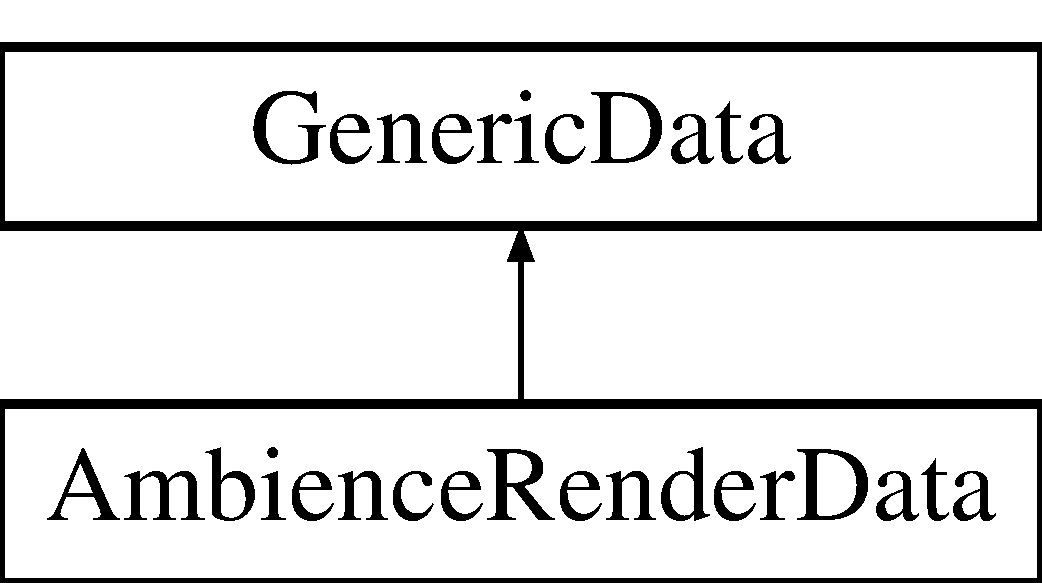
\includegraphics[height=2.000000cm]{class_ambience_render_data}
\end{center}
\end{figure}
\subsection*{Public Member Functions}
\begin{DoxyCompactItemize}
\item 
\hyperlink{class_ambience_render_data_a5590468febae461c201a64313f6c38be}{Ambience\-Render\-Data} (std\-::string filename)
\item 
\hyperlink{class_ambience_render_data_a5905531cc042e53c6c6730e74b8e2325}{Ambience\-Render\-Data} ()
\item 
\hyperlink{class_ambience_render_data_abf7ae51efd4286b33be9aa960dc1f228}{$\sim$\-Ambience\-Render\-Data} ()
\item 
virtual void \hyperlink{class_ambience_render_data_a04e058a2c8b174def8c381a19ede0d12}{write} (std\-::ostream \&out) const 
\item 
virtual void \hyperlink{class_ambience_render_data_a051acf84a9c31c6e439e7d7e7445ef47}{read} (std\-::istream \&in)
\end{DoxyCompactItemize}
\subsection*{Public Attributes}
\begin{DoxyCompactItemize}
\item 
double \hyperlink{class_ambience_render_data_a619be04e63ef41deac443cabba9c8d2f}{m\-Skybox\-Size}
\item 
std\-::string \hyperlink{class_ambience_render_data_a462dce5cb2e535c15a0fbf94d99220e3}{m\-Skybox\-Filename}
\item 
std\-::string \hyperlink{class_ambience_render_data_a642bc5ab8f0db9224f7b00b9d6c58beb}{m\-Terrain\-Texture\-Filename}
\item 
double \hyperlink{class_ambience_render_data_a05eaae9de570dab5a7bce2454b257945}{m\-Terrain\-Meters\-Per\-Image\-X}
\item 
double \hyperlink{class_ambience_render_data_a0ad3dba20cdff18a2de47a305399c72e}{m\-Terrain\-Meters\-Per\-Image\-Y}
\item 
double \hyperlink{class_ambience_render_data_ab897015a20e658f3a8cf9c4b87bcb442}{m\-Terrain\-Speed\-X}
\item 
double \hyperlink{class_ambience_render_data_a09b0e2e8506ffe824a2ffec40471e827}{m\-Terrain\-Speed\-Y}
\item 
double \hyperlink{class_ambience_render_data_a18b979f952900e973802f2d4cca82b13}{m\-Terrain\-Depth}
\end{DoxyCompactItemize}


\subsection{Constructor \& Destructor Documentation}
\hypertarget{class_ambience_render_data_a5590468febae461c201a64313f6c38be}{\index{Ambience\-Render\-Data@{Ambience\-Render\-Data}!Ambience\-Render\-Data@{Ambience\-Render\-Data}}
\index{Ambience\-Render\-Data@{Ambience\-Render\-Data}!AmbienceRenderData@{Ambience\-Render\-Data}}
\subsubsection[{Ambience\-Render\-Data}]{\setlength{\rightskip}{0pt plus 5cm}Ambience\-Render\-Data\-::\-Ambience\-Render\-Data (
\begin{DoxyParamCaption}
\item[{std\-::string}]{filename}
\end{DoxyParamCaption}
)}}\label{class_ambience_render_data_a5590468febae461c201a64313f6c38be}
\hypertarget{class_ambience_render_data_a5905531cc042e53c6c6730e74b8e2325}{\index{Ambience\-Render\-Data@{Ambience\-Render\-Data}!Ambience\-Render\-Data@{Ambience\-Render\-Data}}
\index{Ambience\-Render\-Data@{Ambience\-Render\-Data}!AmbienceRenderData@{Ambience\-Render\-Data}}
\subsubsection[{Ambience\-Render\-Data}]{\setlength{\rightskip}{0pt plus 5cm}Ambience\-Render\-Data\-::\-Ambience\-Render\-Data (
\begin{DoxyParamCaption}
{}
\end{DoxyParamCaption}
)}}\label{class_ambience_render_data_a5905531cc042e53c6c6730e74b8e2325}
\hypertarget{class_ambience_render_data_abf7ae51efd4286b33be9aa960dc1f228}{\index{Ambience\-Render\-Data@{Ambience\-Render\-Data}!$\sim$\-Ambience\-Render\-Data@{$\sim$\-Ambience\-Render\-Data}}
\index{$\sim$\-Ambience\-Render\-Data@{$\sim$\-Ambience\-Render\-Data}!AmbienceRenderData@{Ambience\-Render\-Data}}
\subsubsection[{$\sim$\-Ambience\-Render\-Data}]{\setlength{\rightskip}{0pt plus 5cm}Ambience\-Render\-Data\-::$\sim$\-Ambience\-Render\-Data (
\begin{DoxyParamCaption}
{}
\end{DoxyParamCaption}
)}}\label{class_ambience_render_data_abf7ae51efd4286b33be9aa960dc1f228}


\subsection{Member Function Documentation}
\hypertarget{class_ambience_render_data_a051acf84a9c31c6e439e7d7e7445ef47}{\index{Ambience\-Render\-Data@{Ambience\-Render\-Data}!read@{read}}
\index{read@{read}!AmbienceRenderData@{Ambience\-Render\-Data}}
\subsubsection[{read}]{\setlength{\rightskip}{0pt plus 5cm}void Ambience\-Render\-Data\-::read (
\begin{DoxyParamCaption}
\item[{std\-::istream \&}]{in}
\end{DoxyParamCaption}
)\hspace{0.3cm}{\ttfamily [virtual]}}}\label{class_ambience_render_data_a051acf84a9c31c6e439e7d7e7445ef47}


Implements \hyperlink{class_generic_data_a71e231ef04c9a91a3429123dab5bd1e7}{Generic\-Data}.

\hypertarget{class_ambience_render_data_a04e058a2c8b174def8c381a19ede0d12}{\index{Ambience\-Render\-Data@{Ambience\-Render\-Data}!write@{write}}
\index{write@{write}!AmbienceRenderData@{Ambience\-Render\-Data}}
\subsubsection[{write}]{\setlength{\rightskip}{0pt plus 5cm}void Ambience\-Render\-Data\-::write (
\begin{DoxyParamCaption}
\item[{std\-::ostream \&}]{out}
\end{DoxyParamCaption}
) const\hspace{0.3cm}{\ttfamily [virtual]}}}\label{class_ambience_render_data_a04e058a2c8b174def8c381a19ede0d12}


Implements \hyperlink{class_generic_data_a93ea61de5b09cf3fc95564ef3d841214}{Generic\-Data}.



\subsection{Member Data Documentation}
\hypertarget{class_ambience_render_data_a462dce5cb2e535c15a0fbf94d99220e3}{\index{Ambience\-Render\-Data@{Ambience\-Render\-Data}!m\-Skybox\-Filename@{m\-Skybox\-Filename}}
\index{m\-Skybox\-Filename@{m\-Skybox\-Filename}!AmbienceRenderData@{Ambience\-Render\-Data}}
\subsubsection[{m\-Skybox\-Filename}]{\setlength{\rightskip}{0pt plus 5cm}std\-::string Ambience\-Render\-Data\-::m\-Skybox\-Filename}}\label{class_ambience_render_data_a462dce5cb2e535c15a0fbf94d99220e3}
\hypertarget{class_ambience_render_data_a619be04e63ef41deac443cabba9c8d2f}{\index{Ambience\-Render\-Data@{Ambience\-Render\-Data}!m\-Skybox\-Size@{m\-Skybox\-Size}}
\index{m\-Skybox\-Size@{m\-Skybox\-Size}!AmbienceRenderData@{Ambience\-Render\-Data}}
\subsubsection[{m\-Skybox\-Size}]{\setlength{\rightskip}{0pt plus 5cm}double Ambience\-Render\-Data\-::m\-Skybox\-Size}}\label{class_ambience_render_data_a619be04e63ef41deac443cabba9c8d2f}
\hypertarget{class_ambience_render_data_a18b979f952900e973802f2d4cca82b13}{\index{Ambience\-Render\-Data@{Ambience\-Render\-Data}!m\-Terrain\-Depth@{m\-Terrain\-Depth}}
\index{m\-Terrain\-Depth@{m\-Terrain\-Depth}!AmbienceRenderData@{Ambience\-Render\-Data}}
\subsubsection[{m\-Terrain\-Depth}]{\setlength{\rightskip}{0pt plus 5cm}double Ambience\-Render\-Data\-::m\-Terrain\-Depth}}\label{class_ambience_render_data_a18b979f952900e973802f2d4cca82b13}
\hypertarget{class_ambience_render_data_a05eaae9de570dab5a7bce2454b257945}{\index{Ambience\-Render\-Data@{Ambience\-Render\-Data}!m\-Terrain\-Meters\-Per\-Image\-X@{m\-Terrain\-Meters\-Per\-Image\-X}}
\index{m\-Terrain\-Meters\-Per\-Image\-X@{m\-Terrain\-Meters\-Per\-Image\-X}!AmbienceRenderData@{Ambience\-Render\-Data}}
\subsubsection[{m\-Terrain\-Meters\-Per\-Image\-X}]{\setlength{\rightskip}{0pt plus 5cm}double Ambience\-Render\-Data\-::m\-Terrain\-Meters\-Per\-Image\-X}}\label{class_ambience_render_data_a05eaae9de570dab5a7bce2454b257945}
\hypertarget{class_ambience_render_data_a0ad3dba20cdff18a2de47a305399c72e}{\index{Ambience\-Render\-Data@{Ambience\-Render\-Data}!m\-Terrain\-Meters\-Per\-Image\-Y@{m\-Terrain\-Meters\-Per\-Image\-Y}}
\index{m\-Terrain\-Meters\-Per\-Image\-Y@{m\-Terrain\-Meters\-Per\-Image\-Y}!AmbienceRenderData@{Ambience\-Render\-Data}}
\subsubsection[{m\-Terrain\-Meters\-Per\-Image\-Y}]{\setlength{\rightskip}{0pt plus 5cm}double Ambience\-Render\-Data\-::m\-Terrain\-Meters\-Per\-Image\-Y}}\label{class_ambience_render_data_a0ad3dba20cdff18a2de47a305399c72e}
\hypertarget{class_ambience_render_data_ab897015a20e658f3a8cf9c4b87bcb442}{\index{Ambience\-Render\-Data@{Ambience\-Render\-Data}!m\-Terrain\-Speed\-X@{m\-Terrain\-Speed\-X}}
\index{m\-Terrain\-Speed\-X@{m\-Terrain\-Speed\-X}!AmbienceRenderData@{Ambience\-Render\-Data}}
\subsubsection[{m\-Terrain\-Speed\-X}]{\setlength{\rightskip}{0pt plus 5cm}double Ambience\-Render\-Data\-::m\-Terrain\-Speed\-X}}\label{class_ambience_render_data_ab897015a20e658f3a8cf9c4b87bcb442}
\hypertarget{class_ambience_render_data_a09b0e2e8506ffe824a2ffec40471e827}{\index{Ambience\-Render\-Data@{Ambience\-Render\-Data}!m\-Terrain\-Speed\-Y@{m\-Terrain\-Speed\-Y}}
\index{m\-Terrain\-Speed\-Y@{m\-Terrain\-Speed\-Y}!AmbienceRenderData@{Ambience\-Render\-Data}}
\subsubsection[{m\-Terrain\-Speed\-Y}]{\setlength{\rightskip}{0pt plus 5cm}double Ambience\-Render\-Data\-::m\-Terrain\-Speed\-Y}}\label{class_ambience_render_data_a09b0e2e8506ffe824a2ffec40471e827}
\hypertarget{class_ambience_render_data_a642bc5ab8f0db9224f7b00b9d6c58beb}{\index{Ambience\-Render\-Data@{Ambience\-Render\-Data}!m\-Terrain\-Texture\-Filename@{m\-Terrain\-Texture\-Filename}}
\index{m\-Terrain\-Texture\-Filename@{m\-Terrain\-Texture\-Filename}!AmbienceRenderData@{Ambience\-Render\-Data}}
\subsubsection[{m\-Terrain\-Texture\-Filename}]{\setlength{\rightskip}{0pt plus 5cm}std\-::string Ambience\-Render\-Data\-::m\-Terrain\-Texture\-Filename}}\label{class_ambience_render_data_a642bc5ab8f0db9224f7b00b9d6c58beb}


The documentation for this class was generated from the following files\-:\begin{DoxyCompactItemize}
\item 
C\-:/\-Users/\-Owner/\-My Programming/\-Personal Projects/\-Video\-Games/\-Optimist Racing/src/\hyperlink{_data_8hpp}{Data.\-hpp}\item 
C\-:/\-Users/\-Owner/\-My Programming/\-Personal Projects/\-Video\-Games/\-Optimist Racing/src/\hyperlink{_data_8cpp}{Data.\-cpp}\end{DoxyCompactItemize}

\hypertarget{class_bernstein_polynomial}{\section{Bernstein\-Polynomial Class Reference}
\label{class_bernstein_polynomial}\index{Bernstein\-Polynomial@{Bernstein\-Polynomial}}
}


{\ttfamily \#include $<$Bezier.\-hpp$>$}

\subsection*{Public Member Functions}
\begin{DoxyCompactItemize}
\item 
\hyperlink{class_bernstein_polynomial_a518fdef975c92857e34fa17077b0351a}{Bernstein\-Polynomial} (unsigned int degree)
\item 
\hyperlink{class_bernstein_polynomial_a9b74fd40365e53a1a0fd7de30d688ce0}{$\sim$\-Bernstein\-Polynomial} ()
\item 
unsigned int \hyperlink{class_bernstein_polynomial_af121be73ab75d393d0344311810a9f66}{get\-D} () const 
\item 
\hyperlink{class_matrix_mx_n}{Matrix\-Mx\-N} \hyperlink{class_bernstein_polynomial_ae4dc99cf3e2ea03671ca459dffa02314}{compute} (double t) const 
\item 
\hyperlink{class_matrix_mx_n}{Matrix\-Mx\-N} \hyperlink{class_bernstein_polynomial_a0f7c4c41e6c7d6258eac0ca090a621ea}{compute\-F\-Only} (double t) const 
\end{DoxyCompactItemize}


\subsection{Constructor \& Destructor Documentation}
\hypertarget{class_bernstein_polynomial_a518fdef975c92857e34fa17077b0351a}{\index{Bernstein\-Polynomial@{Bernstein\-Polynomial}!Bernstein\-Polynomial@{Bernstein\-Polynomial}}
\index{Bernstein\-Polynomial@{Bernstein\-Polynomial}!BernsteinPolynomial@{Bernstein\-Polynomial}}
\subsubsection[{Bernstein\-Polynomial}]{\setlength{\rightskip}{0pt plus 5cm}Bernstein\-Polynomial\-::\-Bernstein\-Polynomial (
\begin{DoxyParamCaption}
\item[{unsigned int}]{degree}
\end{DoxyParamCaption}
)}}\label{class_bernstein_polynomial_a518fdef975c92857e34fa17077b0351a}
\hypertarget{class_bernstein_polynomial_a9b74fd40365e53a1a0fd7de30d688ce0}{\index{Bernstein\-Polynomial@{Bernstein\-Polynomial}!$\sim$\-Bernstein\-Polynomial@{$\sim$\-Bernstein\-Polynomial}}
\index{$\sim$\-Bernstein\-Polynomial@{$\sim$\-Bernstein\-Polynomial}!BernsteinPolynomial@{Bernstein\-Polynomial}}
\subsubsection[{$\sim$\-Bernstein\-Polynomial}]{\setlength{\rightskip}{0pt plus 5cm}Bernstein\-Polynomial\-::$\sim$\-Bernstein\-Polynomial (
\begin{DoxyParamCaption}
{}
\end{DoxyParamCaption}
)}}\label{class_bernstein_polynomial_a9b74fd40365e53a1a0fd7de30d688ce0}


\subsection{Member Function Documentation}
\hypertarget{class_bernstein_polynomial_ae4dc99cf3e2ea03671ca459dffa02314}{\index{Bernstein\-Polynomial@{Bernstein\-Polynomial}!compute@{compute}}
\index{compute@{compute}!BernsteinPolynomial@{Bernstein\-Polynomial}}
\subsubsection[{compute}]{\setlength{\rightskip}{0pt plus 5cm}{\bf Matrix\-Mx\-N} Bernstein\-Polynomial\-::compute (
\begin{DoxyParamCaption}
\item[{double}]{t}
\end{DoxyParamCaption}
) const}}\label{class_bernstein_polynomial_ae4dc99cf3e2ea03671ca459dffa02314}
\hypertarget{class_bernstein_polynomial_a0f7c4c41e6c7d6258eac0ca090a621ea}{\index{Bernstein\-Polynomial@{Bernstein\-Polynomial}!compute\-F\-Only@{compute\-F\-Only}}
\index{compute\-F\-Only@{compute\-F\-Only}!BernsteinPolynomial@{Bernstein\-Polynomial}}
\subsubsection[{compute\-F\-Only}]{\setlength{\rightskip}{0pt plus 5cm}{\bf Matrix\-Mx\-N} Bernstein\-Polynomial\-::compute\-F\-Only (
\begin{DoxyParamCaption}
\item[{double}]{t}
\end{DoxyParamCaption}
) const}}\label{class_bernstein_polynomial_a0f7c4c41e6c7d6258eac0ca090a621ea}
\hypertarget{class_bernstein_polynomial_af121be73ab75d393d0344311810a9f66}{\index{Bernstein\-Polynomial@{Bernstein\-Polynomial}!get\-D@{get\-D}}
\index{get\-D@{get\-D}!BernsteinPolynomial@{Bernstein\-Polynomial}}
\subsubsection[{get\-D}]{\setlength{\rightskip}{0pt plus 5cm}unsigned int Bernstein\-Polynomial\-::get\-D (
\begin{DoxyParamCaption}
{}
\end{DoxyParamCaption}
) const}}\label{class_bernstein_polynomial_af121be73ab75d393d0344311810a9f66}


The documentation for this class was generated from the following files\-:\begin{DoxyCompactItemize}
\item 
C\-:/\-Users/\-Owner/\-My Programming/\-Personal Projects/\-Video\-Games/\-Optimist Racing/src/\hyperlink{_bezier_8hpp}{Bezier.\-hpp}\item 
C\-:/\-Users/\-Owner/\-My Programming/\-Personal Projects/\-Video\-Games/\-Optimist Racing/src/\hyperlink{_bezier_8cpp}{Bezier.\-cpp}\end{DoxyCompactItemize}

\hypertarget{class_bezier_patch}{\section{Bezier\-Patch Class Reference}
\label{class_bezier_patch}\index{Bezier\-Patch@{Bezier\-Patch}}
}


{\ttfamily \#include $<$Bezier.\-hpp$>$}

\subsection*{Public Member Functions}
\begin{DoxyCompactItemize}
\item 
\hyperlink{class_bezier_patch_a50506bb4f40a7a537637a114a77d844e}{Bezier\-Patch} (const \hyperlink{class_bernstein_polynomial}{Bernstein\-Polynomial} $\ast$B\-P)
\item 
\hyperlink{class_bezier_patch_ae562d080e4f57c1aef0a8f19adcc4133}{Bezier\-Patch} (const \hyperlink{class_bernstein_polynomial}{Bernstein\-Polynomial} $\ast$B\-P, \hyperlink{class_matrix_mx_n}{Matrix\-Mx\-N} K)
\item 
\hyperlink{class_bezier_patch_ab5b226280fc0afba7e6f21b72423dc8c}{Bezier\-Patch} (const \hyperlink{class_bernstein_polynomial}{Bernstein\-Polynomial} $\ast$B\-P, const \hyperlink{class_matrix_mx_n}{Matrix\-Mx\-N} \&B\-Tilda\-Inv0, const \hyperlink{class_matrix_mx_n}{Matrix\-Mx\-N} \&B\-Tilda\-Inv1, const \hyperlink{class_matrix_mx_n}{Matrix\-Mx\-N} \&f00, const \hyperlink{class_matrix_mx_n}{Matrix\-Mx\-N} \&f01, const \hyperlink{class_matrix_mx_n}{Matrix\-Mx\-N} \&f10, const \hyperlink{class_matrix_mx_n}{Matrix\-Mx\-N} \&f11)
\item 
\hyperlink{class_bezier_patch_aefc712578c4818d622d8a9f623786746}{$\sim$\-Bezier\-Patch} ()
\item 
const \hyperlink{class_matrix_mx_n}{Matrix\-Mx\-N} \& \hyperlink{class_bezier_patch_a32759c1605c0bd966ce87b6cf65bdd8f}{get\-K} () const 
\item 
const \hyperlink{class_bernstein_polynomial}{Bernstein\-Polynomial} $\ast$ \hyperlink{class_bezier_patch_ab5ae6752b90f10228c98948d1184a1bb}{get\-B\-P} () const 
\item 
\hyperlink{class_matrix_mx_n}{Matrix\-Mx\-N} \hyperlink{class_bezier_patch_a850bc5e09dfc474180f4bda49ddb6141}{compute} (double x, double y) const 
\item 
double \hyperlink{class_bezier_patch_af70a22fab5c247edfa5b5b2a762dac4c}{compute\-F\-Only} (double x, double y) const 
\end{DoxyCompactItemize}


\subsection{Constructor \& Destructor Documentation}
\hypertarget{class_bezier_patch_a50506bb4f40a7a537637a114a77d844e}{\index{Bezier\-Patch@{Bezier\-Patch}!Bezier\-Patch@{Bezier\-Patch}}
\index{Bezier\-Patch@{Bezier\-Patch}!BezierPatch@{Bezier\-Patch}}
\subsubsection[{Bezier\-Patch}]{\setlength{\rightskip}{0pt plus 5cm}Bezier\-Patch\-::\-Bezier\-Patch (
\begin{DoxyParamCaption}
\item[{const {\bf Bernstein\-Polynomial} $\ast$}]{B\-P}
\end{DoxyParamCaption}
)}}\label{class_bezier_patch_a50506bb4f40a7a537637a114a77d844e}
\hypertarget{class_bezier_patch_ae562d080e4f57c1aef0a8f19adcc4133}{\index{Bezier\-Patch@{Bezier\-Patch}!Bezier\-Patch@{Bezier\-Patch}}
\index{Bezier\-Patch@{Bezier\-Patch}!BezierPatch@{Bezier\-Patch}}
\subsubsection[{Bezier\-Patch}]{\setlength{\rightskip}{0pt plus 5cm}Bezier\-Patch\-::\-Bezier\-Patch (
\begin{DoxyParamCaption}
\item[{const {\bf Bernstein\-Polynomial} $\ast$}]{B\-P, }
\item[{{\bf Matrix\-Mx\-N}}]{K}
\end{DoxyParamCaption}
)}}\label{class_bezier_patch_ae562d080e4f57c1aef0a8f19adcc4133}
\hypertarget{class_bezier_patch_ab5b226280fc0afba7e6f21b72423dc8c}{\index{Bezier\-Patch@{Bezier\-Patch}!Bezier\-Patch@{Bezier\-Patch}}
\index{Bezier\-Patch@{Bezier\-Patch}!BezierPatch@{Bezier\-Patch}}
\subsubsection[{Bezier\-Patch}]{\setlength{\rightskip}{0pt plus 5cm}Bezier\-Patch\-::\-Bezier\-Patch (
\begin{DoxyParamCaption}
\item[{const {\bf Bernstein\-Polynomial} $\ast$}]{B\-P, }
\item[{const {\bf Matrix\-Mx\-N} \&}]{B\-Tilda\-Inv0, }
\item[{const {\bf Matrix\-Mx\-N} \&}]{B\-Tilda\-Inv1, }
\item[{const {\bf Matrix\-Mx\-N} \&}]{f00, }
\item[{const {\bf Matrix\-Mx\-N} \&}]{f01, }
\item[{const {\bf Matrix\-Mx\-N} \&}]{f10, }
\item[{const {\bf Matrix\-Mx\-N} \&}]{f11}
\end{DoxyParamCaption}
)}}\label{class_bezier_patch_ab5b226280fc0afba7e6f21b72423dc8c}
\hypertarget{class_bezier_patch_aefc712578c4818d622d8a9f623786746}{\index{Bezier\-Patch@{Bezier\-Patch}!$\sim$\-Bezier\-Patch@{$\sim$\-Bezier\-Patch}}
\index{$\sim$\-Bezier\-Patch@{$\sim$\-Bezier\-Patch}!BezierPatch@{Bezier\-Patch}}
\subsubsection[{$\sim$\-Bezier\-Patch}]{\setlength{\rightskip}{0pt plus 5cm}Bezier\-Patch\-::$\sim$\-Bezier\-Patch (
\begin{DoxyParamCaption}
{}
\end{DoxyParamCaption}
)}}\label{class_bezier_patch_aefc712578c4818d622d8a9f623786746}


\subsection{Member Function Documentation}
\hypertarget{class_bezier_patch_a850bc5e09dfc474180f4bda49ddb6141}{\index{Bezier\-Patch@{Bezier\-Patch}!compute@{compute}}
\index{compute@{compute}!BezierPatch@{Bezier\-Patch}}
\subsubsection[{compute}]{\setlength{\rightskip}{0pt plus 5cm}{\bf Matrix\-Mx\-N} Bezier\-Patch\-::compute (
\begin{DoxyParamCaption}
\item[{double}]{x, }
\item[{double}]{y}
\end{DoxyParamCaption}
) const}}\label{class_bezier_patch_a850bc5e09dfc474180f4bda49ddb6141}
\hypertarget{class_bezier_patch_af70a22fab5c247edfa5b5b2a762dac4c}{\index{Bezier\-Patch@{Bezier\-Patch}!compute\-F\-Only@{compute\-F\-Only}}
\index{compute\-F\-Only@{compute\-F\-Only}!BezierPatch@{Bezier\-Patch}}
\subsubsection[{compute\-F\-Only}]{\setlength{\rightskip}{0pt plus 5cm}double Bezier\-Patch\-::compute\-F\-Only (
\begin{DoxyParamCaption}
\item[{double}]{x, }
\item[{double}]{y}
\end{DoxyParamCaption}
) const}}\label{class_bezier_patch_af70a22fab5c247edfa5b5b2a762dac4c}
\hypertarget{class_bezier_patch_ab5ae6752b90f10228c98948d1184a1bb}{\index{Bezier\-Patch@{Bezier\-Patch}!get\-B\-P@{get\-B\-P}}
\index{get\-B\-P@{get\-B\-P}!BezierPatch@{Bezier\-Patch}}
\subsubsection[{get\-B\-P}]{\setlength{\rightskip}{0pt plus 5cm}const {\bf Bernstein\-Polynomial} $\ast$ Bezier\-Patch\-::get\-B\-P (
\begin{DoxyParamCaption}
{}
\end{DoxyParamCaption}
) const}}\label{class_bezier_patch_ab5ae6752b90f10228c98948d1184a1bb}
\hypertarget{class_bezier_patch_a32759c1605c0bd966ce87b6cf65bdd8f}{\index{Bezier\-Patch@{Bezier\-Patch}!get\-K@{get\-K}}
\index{get\-K@{get\-K}!BezierPatch@{Bezier\-Patch}}
\subsubsection[{get\-K}]{\setlength{\rightskip}{0pt plus 5cm}const {\bf Matrix\-Mx\-N} \& Bezier\-Patch\-::get\-K (
\begin{DoxyParamCaption}
{}
\end{DoxyParamCaption}
) const}}\label{class_bezier_patch_a32759c1605c0bd966ce87b6cf65bdd8f}


The documentation for this class was generated from the following files\-:\begin{DoxyCompactItemize}
\item 
C\-:/\-Users/\-Owner/\-My Programming/\-Personal Projects/\-Video\-Games/\-Optimist Racing/src/\hyperlink{_bezier_8hpp}{Bezier.\-hpp}\item 
C\-:/\-Users/\-Owner/\-My Programming/\-Personal Projects/\-Video\-Games/\-Optimist Racing/src/\hyperlink{_bezier_8cpp}{Bezier.\-cpp}\end{DoxyCompactItemize}

\hypertarget{class_bezier_patch_grid}{\section{Bezier\-Patch\-Grid Class Reference}
\label{class_bezier_patch_grid}\index{Bezier\-Patch\-Grid@{Bezier\-Patch\-Grid}}
}


{\ttfamily \#include $<$Bezier.\-hpp$>$}

\subsection*{Public Member Functions}
\begin{DoxyCompactItemize}
\item 
\hyperlink{class_bezier_patch_grid_a554a55115356412abc18baec436188be}{Bezier\-Patch\-Grid} (const \hyperlink{class_bernstein_polynomial}{Bernstein\-Polynomial} $\ast$B\-P, double grid\-Hx, double grid\-Hy, unsigned int num\-Cells\-X, unsigned int num\-Cells\-Y, \hyperlink{class_matrix_mx_n}{Matrix\-Mx\-N} $\ast$$\ast$corners)
\item 
\hyperlink{class_bezier_patch_grid_a2d05668c85a89cc22ecec7527dc61fb6}{$\sim$\-Bezier\-Patch\-Grid} ()
\item 
double \hyperlink{class_bezier_patch_grid_a097dc86c745cf672dae184ba638a575f}{get\-Grid\-H\-X} () const 
\item 
double \hyperlink{class_bezier_patch_grid_a415ab4140e78d397cf102ec7a349c858}{get\-Grid\-H\-Y} () const 
\item 
unsigned int \hyperlink{class_bezier_patch_grid_a68d5e67e34eb2290e3dc66aad978003a}{get\-Num\-Cells\-X} () const 
\item 
unsigned int \hyperlink{class_bezier_patch_grid_a527f5f89d884c8c496b87cd733bd5e57}{get\-Num\-Cells\-Y} () const 
\item 
const \hyperlink{class_bezier_patch}{Bezier\-Patch} \& \hyperlink{class_bezier_patch_grid_a9e9c8bbdad683ca8a9afba393c105223}{get\-Patch} (unsigned int x, unsigned int y) const 
\item 
\hyperlink{class_matrix_mx_n}{Matrix\-Mx\-N} \hyperlink{class_bezier_patch_grid_a255a33e2613464997d2afee32bc549ab}{compute} (double x, double y) const 
\item 
double \hyperlink{class_bezier_patch_grid_afa4d08b2c4e00e9e9a068b5bff86951f}{compute\-F\-Only} (double x, double y) const 
\end{DoxyCompactItemize}


\subsection{Constructor \& Destructor Documentation}
\hypertarget{class_bezier_patch_grid_a554a55115356412abc18baec436188be}{\index{Bezier\-Patch\-Grid@{Bezier\-Patch\-Grid}!Bezier\-Patch\-Grid@{Bezier\-Patch\-Grid}}
\index{Bezier\-Patch\-Grid@{Bezier\-Patch\-Grid}!BezierPatchGrid@{Bezier\-Patch\-Grid}}
\subsubsection[{Bezier\-Patch\-Grid}]{\setlength{\rightskip}{0pt plus 5cm}Bezier\-Patch\-Grid\-::\-Bezier\-Patch\-Grid (
\begin{DoxyParamCaption}
\item[{const {\bf Bernstein\-Polynomial} $\ast$}]{B\-P, }
\item[{double}]{grid\-Hx, }
\item[{double}]{grid\-Hy, }
\item[{unsigned int}]{num\-Cells\-X, }
\item[{unsigned int}]{num\-Cells\-Y, }
\item[{{\bf Matrix\-Mx\-N} $\ast$$\ast$}]{corners}
\end{DoxyParamCaption}
)}}\label{class_bezier_patch_grid_a554a55115356412abc18baec436188be}
\hypertarget{class_bezier_patch_grid_a2d05668c85a89cc22ecec7527dc61fb6}{\index{Bezier\-Patch\-Grid@{Bezier\-Patch\-Grid}!$\sim$\-Bezier\-Patch\-Grid@{$\sim$\-Bezier\-Patch\-Grid}}
\index{$\sim$\-Bezier\-Patch\-Grid@{$\sim$\-Bezier\-Patch\-Grid}!BezierPatchGrid@{Bezier\-Patch\-Grid}}
\subsubsection[{$\sim$\-Bezier\-Patch\-Grid}]{\setlength{\rightskip}{0pt plus 5cm}Bezier\-Patch\-Grid\-::$\sim$\-Bezier\-Patch\-Grid (
\begin{DoxyParamCaption}
{}
\end{DoxyParamCaption}
)}}\label{class_bezier_patch_grid_a2d05668c85a89cc22ecec7527dc61fb6}


\subsection{Member Function Documentation}
\hypertarget{class_bezier_patch_grid_a255a33e2613464997d2afee32bc549ab}{\index{Bezier\-Patch\-Grid@{Bezier\-Patch\-Grid}!compute@{compute}}
\index{compute@{compute}!BezierPatchGrid@{Bezier\-Patch\-Grid}}
\subsubsection[{compute}]{\setlength{\rightskip}{0pt plus 5cm}{\bf Matrix\-Mx\-N} Bezier\-Patch\-Grid\-::compute (
\begin{DoxyParamCaption}
\item[{double}]{x, }
\item[{double}]{y}
\end{DoxyParamCaption}
) const}}\label{class_bezier_patch_grid_a255a33e2613464997d2afee32bc549ab}
\hypertarget{class_bezier_patch_grid_afa4d08b2c4e00e9e9a068b5bff86951f}{\index{Bezier\-Patch\-Grid@{Bezier\-Patch\-Grid}!compute\-F\-Only@{compute\-F\-Only}}
\index{compute\-F\-Only@{compute\-F\-Only}!BezierPatchGrid@{Bezier\-Patch\-Grid}}
\subsubsection[{compute\-F\-Only}]{\setlength{\rightskip}{0pt plus 5cm}double Bezier\-Patch\-Grid\-::compute\-F\-Only (
\begin{DoxyParamCaption}
\item[{double}]{x, }
\item[{double}]{y}
\end{DoxyParamCaption}
) const}}\label{class_bezier_patch_grid_afa4d08b2c4e00e9e9a068b5bff86951f}
\hypertarget{class_bezier_patch_grid_a097dc86c745cf672dae184ba638a575f}{\index{Bezier\-Patch\-Grid@{Bezier\-Patch\-Grid}!get\-Grid\-H\-X@{get\-Grid\-H\-X}}
\index{get\-Grid\-H\-X@{get\-Grid\-H\-X}!BezierPatchGrid@{Bezier\-Patch\-Grid}}
\subsubsection[{get\-Grid\-H\-X}]{\setlength{\rightskip}{0pt plus 5cm}double Bezier\-Patch\-Grid\-::get\-Grid\-H\-X (
\begin{DoxyParamCaption}
{}
\end{DoxyParamCaption}
) const}}\label{class_bezier_patch_grid_a097dc86c745cf672dae184ba638a575f}
\hypertarget{class_bezier_patch_grid_a415ab4140e78d397cf102ec7a349c858}{\index{Bezier\-Patch\-Grid@{Bezier\-Patch\-Grid}!get\-Grid\-H\-Y@{get\-Grid\-H\-Y}}
\index{get\-Grid\-H\-Y@{get\-Grid\-H\-Y}!BezierPatchGrid@{Bezier\-Patch\-Grid}}
\subsubsection[{get\-Grid\-H\-Y}]{\setlength{\rightskip}{0pt plus 5cm}double Bezier\-Patch\-Grid\-::get\-Grid\-H\-Y (
\begin{DoxyParamCaption}
{}
\end{DoxyParamCaption}
) const}}\label{class_bezier_patch_grid_a415ab4140e78d397cf102ec7a349c858}
\hypertarget{class_bezier_patch_grid_a68d5e67e34eb2290e3dc66aad978003a}{\index{Bezier\-Patch\-Grid@{Bezier\-Patch\-Grid}!get\-Num\-Cells\-X@{get\-Num\-Cells\-X}}
\index{get\-Num\-Cells\-X@{get\-Num\-Cells\-X}!BezierPatchGrid@{Bezier\-Patch\-Grid}}
\subsubsection[{get\-Num\-Cells\-X}]{\setlength{\rightskip}{0pt plus 5cm}unsigned int Bezier\-Patch\-Grid\-::get\-Num\-Cells\-X (
\begin{DoxyParamCaption}
{}
\end{DoxyParamCaption}
) const}}\label{class_bezier_patch_grid_a68d5e67e34eb2290e3dc66aad978003a}
\hypertarget{class_bezier_patch_grid_a527f5f89d884c8c496b87cd733bd5e57}{\index{Bezier\-Patch\-Grid@{Bezier\-Patch\-Grid}!get\-Num\-Cells\-Y@{get\-Num\-Cells\-Y}}
\index{get\-Num\-Cells\-Y@{get\-Num\-Cells\-Y}!BezierPatchGrid@{Bezier\-Patch\-Grid}}
\subsubsection[{get\-Num\-Cells\-Y}]{\setlength{\rightskip}{0pt plus 5cm}unsigned int Bezier\-Patch\-Grid\-::get\-Num\-Cells\-Y (
\begin{DoxyParamCaption}
{}
\end{DoxyParamCaption}
) const}}\label{class_bezier_patch_grid_a527f5f89d884c8c496b87cd733bd5e57}
\hypertarget{class_bezier_patch_grid_a9e9c8bbdad683ca8a9afba393c105223}{\index{Bezier\-Patch\-Grid@{Bezier\-Patch\-Grid}!get\-Patch@{get\-Patch}}
\index{get\-Patch@{get\-Patch}!BezierPatchGrid@{Bezier\-Patch\-Grid}}
\subsubsection[{get\-Patch}]{\setlength{\rightskip}{0pt plus 5cm}const {\bf Bezier\-Patch} \& Bezier\-Patch\-Grid\-::get\-Patch (
\begin{DoxyParamCaption}
\item[{unsigned int}]{x, }
\item[{unsigned int}]{y}
\end{DoxyParamCaption}
) const}}\label{class_bezier_patch_grid_a9e9c8bbdad683ca8a9afba393c105223}


The documentation for this class was generated from the following files\-:\begin{DoxyCompactItemize}
\item 
C\-:/\-Users/\-Owner/\-My Programming/\-Personal Projects/\-Video\-Games/\-Optimist Racing/src/\hyperlink{_bezier_8hpp}{Bezier.\-hpp}\item 
C\-:/\-Users/\-Owner/\-My Programming/\-Personal Projects/\-Video\-Games/\-Optimist Racing/src/\hyperlink{_bezier_8cpp}{Bezier.\-cpp}\end{DoxyCompactItemize}

\hypertarget{class_camera}{\section{Camera Class Reference}
\label{class_camera}\index{Camera@{Camera}}
}


{\ttfamily \#include $<$Camera.\-hpp$>$}

Inheritance diagram for Camera\-:\begin{figure}[H]
\begin{center}
\leavevmode
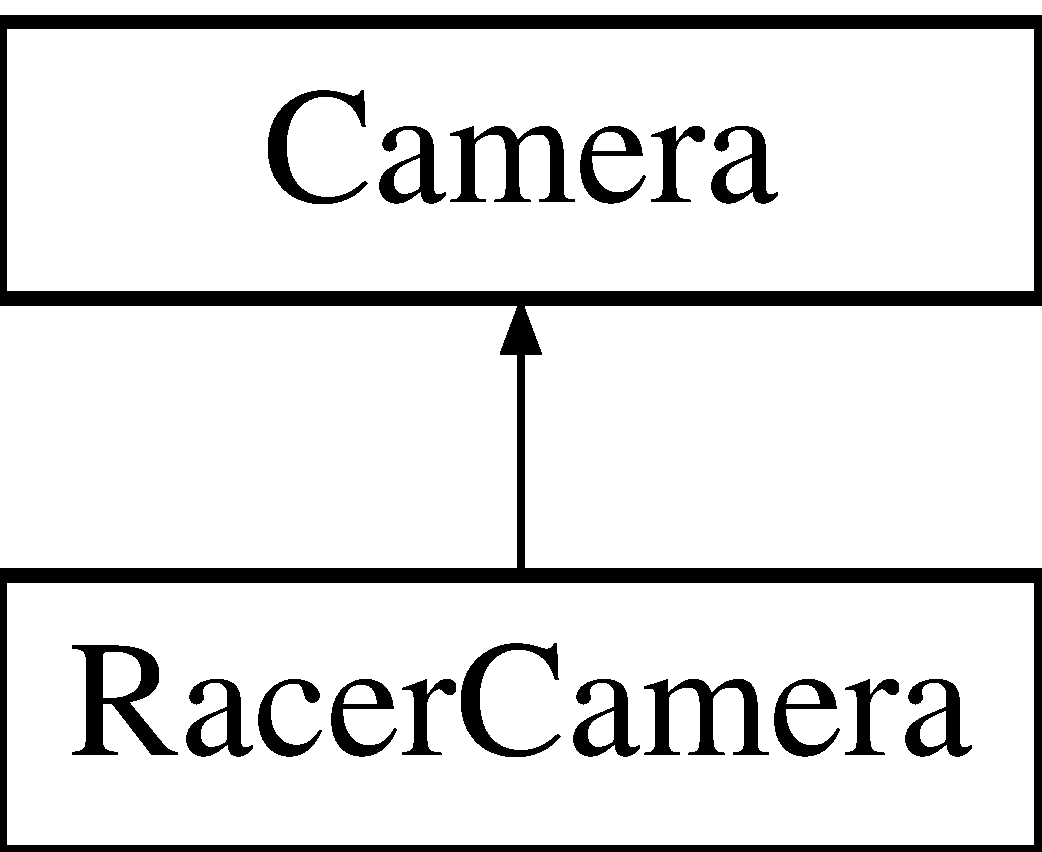
\includegraphics[height=2.000000cm]{class_camera}
\end{center}
\end{figure}
\subsection*{Public Member Functions}
\begin{DoxyCompactItemize}
\item 
\hyperlink{class_camera_a01f94c3543f56ede7af49dc778f19331}{Camera} ()
\item 
\hyperlink{class_camera_ad1897942d0ccf91052386388a497349f}{$\sim$\-Camera} ()
\item 
virtual void \hyperlink{class_camera_af3a878a62730b49ab38b33c75325342e}{gl\-Apply} ()=0
\item 
void \hyperlink{class_camera_a3ad7b867f72a6279f4e19b7dcfb0b071}{freeze} ()
\item 
void \hyperlink{class_camera_a80b6f23356955890272241df1c185379}{unfreeze} ()
\end{DoxyCompactItemize}
\subsection*{Protected Attributes}
\begin{DoxyCompactItemize}
\item 
bool \hyperlink{class_camera_ae2a9a29d6dfb6626c08ecf9b5ed444da}{m\-Freeze}
\item 
\hyperlink{class_vector3_d}{Vector3\-D} \hyperlink{class_camera_a893ec886bbdbc025e54a492b54c585ca}{m\-Position}
\item 
\hyperlink{class_vector3_d}{Vector3\-D} \hyperlink{class_camera_a5569a68f84f82a1fcf128baac654562a}{m\-Up}
\end{DoxyCompactItemize}


\subsection{Detailed Description}
This class is meant to store the position of a camera that doesn't interact physically with the world. Can store position while frozen in space. 

\subsection{Constructor \& Destructor Documentation}
\hypertarget{class_camera_a01f94c3543f56ede7af49dc778f19331}{\index{Camera@{Camera}!Camera@{Camera}}
\index{Camera@{Camera}!Camera@{Camera}}
\subsubsection[{Camera}]{\setlength{\rightskip}{0pt plus 5cm}Camera\-::\-Camera (
\begin{DoxyParamCaption}
{}
\end{DoxyParamCaption}
)}}\label{class_camera_a01f94c3543f56ede7af49dc778f19331}
Basic constructor, begins unfrozen, at the origin, with a standard orientation. \hypertarget{class_camera_ad1897942d0ccf91052386388a497349f}{\index{Camera@{Camera}!$\sim$\-Camera@{$\sim$\-Camera}}
\index{$\sim$\-Camera@{$\sim$\-Camera}!Camera@{Camera}}
\subsubsection[{$\sim$\-Camera}]{\setlength{\rightskip}{0pt plus 5cm}Camera\-::$\sim$\-Camera (
\begin{DoxyParamCaption}
{}
\end{DoxyParamCaption}
)}}\label{class_camera_ad1897942d0ccf91052386388a497349f}
Destructor, does not do anything since it doesn't have to. 

\subsection{Member Function Documentation}
\hypertarget{class_camera_a3ad7b867f72a6279f4e19b7dcfb0b071}{\index{Camera@{Camera}!freeze@{freeze}}
\index{freeze@{freeze}!Camera@{Camera}}
\subsubsection[{freeze}]{\setlength{\rightskip}{0pt plus 5cm}void Camera\-::freeze (
\begin{DoxyParamCaption}
{}
\end{DoxyParamCaption}
)}}\label{class_camera_a3ad7b867f72a6279f4e19b7dcfb0b071}
Freezes the position of the camera, but not its orientation, so that if the point of focus moves, the camera doesn't move with it anymore. \hypertarget{class_camera_af3a878a62730b49ab38b33c75325342e}{\index{Camera@{Camera}!gl\-Apply@{gl\-Apply}}
\index{gl\-Apply@{gl\-Apply}!Camera@{Camera}}
\subsubsection[{gl\-Apply}]{\setlength{\rightskip}{0pt plus 5cm}virtual void Camera\-::gl\-Apply (
\begin{DoxyParamCaption}
{}
\end{DoxyParamCaption}
)\hspace{0.3cm}{\ttfamily [pure virtual]}}}\label{class_camera_af3a878a62730b49ab38b33c75325342e}
Sets up the camera in Open\-G\-L according to the camera's position and orientation. I.\-e. multiplies the transformation matrix in Open\-G\-L by the right translations and rotations. You should usually call this in Model\-View mode before drawing anything. 

Implemented in \hyperlink{class_racer_camera_a5e8a09a6290c7284cfc22ec3a8153dac}{Racer\-Camera}.

\hypertarget{class_camera_a80b6f23356955890272241df1c185379}{\index{Camera@{Camera}!unfreeze@{unfreeze}}
\index{unfreeze@{unfreeze}!Camera@{Camera}}
\subsubsection[{unfreeze}]{\setlength{\rightskip}{0pt plus 5cm}void Camera\-::unfreeze (
\begin{DoxyParamCaption}
{}
\end{DoxyParamCaption}
)}}\label{class_camera_a80b6f23356955890272241df1c185379}
Undoes the effect of the freeze method, so that the camera moves as usual again. 

\subsection{Member Data Documentation}
\hypertarget{class_camera_ae2a9a29d6dfb6626c08ecf9b5ed444da}{\index{Camera@{Camera}!m\-Freeze@{m\-Freeze}}
\index{m\-Freeze@{m\-Freeze}!Camera@{Camera}}
\subsubsection[{m\-Freeze}]{\setlength{\rightskip}{0pt plus 5cm}bool Camera\-::m\-Freeze\hspace{0.3cm}{\ttfamily [protected]}}}\label{class_camera_ae2a9a29d6dfb6626c08ecf9b5ed444da}
\hypertarget{class_camera_a893ec886bbdbc025e54a492b54c585ca}{\index{Camera@{Camera}!m\-Position@{m\-Position}}
\index{m\-Position@{m\-Position}!Camera@{Camera}}
\subsubsection[{m\-Position}]{\setlength{\rightskip}{0pt plus 5cm}{\bf Vector3\-D} Camera\-::m\-Position\hspace{0.3cm}{\ttfamily [protected]}}}\label{class_camera_a893ec886bbdbc025e54a492b54c585ca}
\hypertarget{class_camera_a5569a68f84f82a1fcf128baac654562a}{\index{Camera@{Camera}!m\-Up@{m\-Up}}
\index{m\-Up@{m\-Up}!Camera@{Camera}}
\subsubsection[{m\-Up}]{\setlength{\rightskip}{0pt plus 5cm}{\bf Vector3\-D} Camera\-::m\-Up\hspace{0.3cm}{\ttfamily [protected]}}}\label{class_camera_a5569a68f84f82a1fcf128baac654562a}


The documentation for this class was generated from the following files\-:\begin{DoxyCompactItemize}
\item 
C\-:/\-Users/\-Owner/\-My Programming/\-Personal Projects/\-Video\-Games/\-Optimist Racing/src/\hyperlink{_camera_8hpp}{Camera.\-hpp}\item 
C\-:/\-Users/\-Owner/\-My Programming/\-Personal Projects/\-Video\-Games/\-Optimist Racing/src/\hyperlink{_camera_8cpp}{Camera.\-cpp}\end{DoxyCompactItemize}

\hypertarget{classcm_key_manager}{\section{cm\-Key\-Manager Class Reference}
\label{classcm_key_manager}\index{cm\-Key\-Manager@{cm\-Key\-Manager}}
}


{\ttfamily \#include $<$Keyboard.\-hpp$>$}

\subsection*{Public Member Functions}
\begin{DoxyCompactItemize}
\item 
\hyperlink{classcm_key_manager_a79ae9754c7fe3ea67f6c8184adf90691}{cm\-Key\-Manager} ()
\item 
\hyperlink{classcm_key_manager_a0c96493d3fd7fa83e74dae732cc18df3}{$\sim$cm\-Key\-Manager} ()
\item 
void \hyperlink{classcm_key_manager_abb23711c55b58fed5a85d4ab59b1a8ff}{set\-\_\-mapping} (unsigned char key, \hyperlink{_keyboard_8hpp_ad4a278e59ed8d2af129f9b88eaa342ae}{E\-\_\-\-B\-U\-T\-T\-O\-N} keytype)
\item 
void \hyperlink{classcm_key_manager_aa70f8c04d16bcd19f99dd0117d3b5cd0}{set\-\_\-special\-\_\-mapping} (int key, \hyperlink{_keyboard_8hpp_ad4a278e59ed8d2af129f9b88eaa342ae}{E\-\_\-\-B\-U\-T\-T\-O\-N} keytype)
\item 
void \hyperlink{classcm_key_manager_a62fe4906c92806bafc66f37a5dcd63f1}{press\-\_\-key} (unsigned char key)
\item 
void \hyperlink{classcm_key_manager_ae8f67f69903df93356cf0a36be42f8c2}{press\-\_\-special\-\_\-key} (int key)
\item 
void \hyperlink{classcm_key_manager_a3c3daabf86791170d0db86491dda289c}{release\-\_\-key} (unsigned char key)
\item 
void \hyperlink{classcm_key_manager_ae8f80f4a5ff0a6e11ad0a06fc855a960}{release\-\_\-special\-\_\-key} (int key)
\item 
void \hyperlink{classcm_key_manager_a4a346eef64306328b72f5ce245bf8788}{reset\-\_\-counts} ()
\item 
int \hyperlink{classcm_key_manager_a5fa0ab83e8f36c9a721794c17fb13cb1}{times\-\_\-pressed} (\hyperlink{_keyboard_8hpp_ad4a278e59ed8d2af129f9b88eaa342ae}{E\-\_\-\-B\-U\-T\-T\-O\-N} button) const 
\item 
int \hyperlink{classcm_key_manager_af5d00cb2ad3b1c6350b5486cb2ec27ee}{times\-\_\-released} (\hyperlink{_keyboard_8hpp_ad4a278e59ed8d2af129f9b88eaa342ae}{E\-\_\-\-B\-U\-T\-T\-O\-N} button) const 
\item 
bool \hyperlink{classcm_key_manager_af97cb352de7f7e88efb2beb56a2c68d2}{is\-\_\-pressed} (\hyperlink{_keyboard_8hpp_ad4a278e59ed8d2af129f9b88eaa342ae}{E\-\_\-\-B\-U\-T\-T\-O\-N} button) const 
\end{DoxyCompactItemize}


\subsection{Constructor \& Destructor Documentation}
\hypertarget{classcm_key_manager_a79ae9754c7fe3ea67f6c8184adf90691}{\index{cm\-Key\-Manager@{cm\-Key\-Manager}!cm\-Key\-Manager@{cm\-Key\-Manager}}
\index{cm\-Key\-Manager@{cm\-Key\-Manager}!cmKeyManager@{cm\-Key\-Manager}}
\subsubsection[{cm\-Key\-Manager}]{\setlength{\rightskip}{0pt plus 5cm}cm\-Key\-Manager\-::cm\-Key\-Manager (
\begin{DoxyParamCaption}
{}
\end{DoxyParamCaption}
)}}\label{classcm_key_manager_a79ae9754c7fe3ea67f6c8184adf90691}
\hypertarget{classcm_key_manager_a0c96493d3fd7fa83e74dae732cc18df3}{\index{cm\-Key\-Manager@{cm\-Key\-Manager}!$\sim$cm\-Key\-Manager@{$\sim$cm\-Key\-Manager}}
\index{$\sim$cm\-Key\-Manager@{$\sim$cm\-Key\-Manager}!cmKeyManager@{cm\-Key\-Manager}}
\subsubsection[{$\sim$cm\-Key\-Manager}]{\setlength{\rightskip}{0pt plus 5cm}cm\-Key\-Manager\-::$\sim$cm\-Key\-Manager (
\begin{DoxyParamCaption}
{}
\end{DoxyParamCaption}
)}}\label{classcm_key_manager_a0c96493d3fd7fa83e74dae732cc18df3}


\subsection{Member Function Documentation}
\hypertarget{classcm_key_manager_af97cb352de7f7e88efb2beb56a2c68d2}{\index{cm\-Key\-Manager@{cm\-Key\-Manager}!is\-\_\-pressed@{is\-\_\-pressed}}
\index{is\-\_\-pressed@{is\-\_\-pressed}!cmKeyManager@{cm\-Key\-Manager}}
\subsubsection[{is\-\_\-pressed}]{\setlength{\rightskip}{0pt plus 5cm}bool cm\-Key\-Manager\-::is\-\_\-pressed (
\begin{DoxyParamCaption}
\item[{{\bf E\-\_\-\-B\-U\-T\-T\-O\-N}}]{button}
\end{DoxyParamCaption}
) const}}\label{classcm_key_manager_af97cb352de7f7e88efb2beb56a2c68d2}
\hypertarget{classcm_key_manager_a62fe4906c92806bafc66f37a5dcd63f1}{\index{cm\-Key\-Manager@{cm\-Key\-Manager}!press\-\_\-key@{press\-\_\-key}}
\index{press\-\_\-key@{press\-\_\-key}!cmKeyManager@{cm\-Key\-Manager}}
\subsubsection[{press\-\_\-key}]{\setlength{\rightskip}{0pt plus 5cm}void cm\-Key\-Manager\-::press\-\_\-key (
\begin{DoxyParamCaption}
\item[{unsigned char}]{key}
\end{DoxyParamCaption}
)}}\label{classcm_key_manager_a62fe4906c92806bafc66f37a5dcd63f1}
\hypertarget{classcm_key_manager_ae8f67f69903df93356cf0a36be42f8c2}{\index{cm\-Key\-Manager@{cm\-Key\-Manager}!press\-\_\-special\-\_\-key@{press\-\_\-special\-\_\-key}}
\index{press\-\_\-special\-\_\-key@{press\-\_\-special\-\_\-key}!cmKeyManager@{cm\-Key\-Manager}}
\subsubsection[{press\-\_\-special\-\_\-key}]{\setlength{\rightskip}{0pt plus 5cm}void cm\-Key\-Manager\-::press\-\_\-special\-\_\-key (
\begin{DoxyParamCaption}
\item[{int}]{key}
\end{DoxyParamCaption}
)}}\label{classcm_key_manager_ae8f67f69903df93356cf0a36be42f8c2}
\hypertarget{classcm_key_manager_a3c3daabf86791170d0db86491dda289c}{\index{cm\-Key\-Manager@{cm\-Key\-Manager}!release\-\_\-key@{release\-\_\-key}}
\index{release\-\_\-key@{release\-\_\-key}!cmKeyManager@{cm\-Key\-Manager}}
\subsubsection[{release\-\_\-key}]{\setlength{\rightskip}{0pt plus 5cm}void cm\-Key\-Manager\-::release\-\_\-key (
\begin{DoxyParamCaption}
\item[{unsigned char}]{key}
\end{DoxyParamCaption}
)}}\label{classcm_key_manager_a3c3daabf86791170d0db86491dda289c}
\hypertarget{classcm_key_manager_ae8f80f4a5ff0a6e11ad0a06fc855a960}{\index{cm\-Key\-Manager@{cm\-Key\-Manager}!release\-\_\-special\-\_\-key@{release\-\_\-special\-\_\-key}}
\index{release\-\_\-special\-\_\-key@{release\-\_\-special\-\_\-key}!cmKeyManager@{cm\-Key\-Manager}}
\subsubsection[{release\-\_\-special\-\_\-key}]{\setlength{\rightskip}{0pt plus 5cm}void cm\-Key\-Manager\-::release\-\_\-special\-\_\-key (
\begin{DoxyParamCaption}
\item[{int}]{key}
\end{DoxyParamCaption}
)}}\label{classcm_key_manager_ae8f80f4a5ff0a6e11ad0a06fc855a960}
\hypertarget{classcm_key_manager_a4a346eef64306328b72f5ce245bf8788}{\index{cm\-Key\-Manager@{cm\-Key\-Manager}!reset\-\_\-counts@{reset\-\_\-counts}}
\index{reset\-\_\-counts@{reset\-\_\-counts}!cmKeyManager@{cm\-Key\-Manager}}
\subsubsection[{reset\-\_\-counts}]{\setlength{\rightskip}{0pt plus 5cm}void cm\-Key\-Manager\-::reset\-\_\-counts (
\begin{DoxyParamCaption}
{}
\end{DoxyParamCaption}
)}}\label{classcm_key_manager_a4a346eef64306328b72f5ce245bf8788}
\hypertarget{classcm_key_manager_abb23711c55b58fed5a85d4ab59b1a8ff}{\index{cm\-Key\-Manager@{cm\-Key\-Manager}!set\-\_\-mapping@{set\-\_\-mapping}}
\index{set\-\_\-mapping@{set\-\_\-mapping}!cmKeyManager@{cm\-Key\-Manager}}
\subsubsection[{set\-\_\-mapping}]{\setlength{\rightskip}{0pt plus 5cm}void cm\-Key\-Manager\-::set\-\_\-mapping (
\begin{DoxyParamCaption}
\item[{unsigned char}]{key, }
\item[{{\bf E\-\_\-\-B\-U\-T\-T\-O\-N}}]{keytype}
\end{DoxyParamCaption}
)}}\label{classcm_key_manager_abb23711c55b58fed5a85d4ab59b1a8ff}
\hypertarget{classcm_key_manager_aa70f8c04d16bcd19f99dd0117d3b5cd0}{\index{cm\-Key\-Manager@{cm\-Key\-Manager}!set\-\_\-special\-\_\-mapping@{set\-\_\-special\-\_\-mapping}}
\index{set\-\_\-special\-\_\-mapping@{set\-\_\-special\-\_\-mapping}!cmKeyManager@{cm\-Key\-Manager}}
\subsubsection[{set\-\_\-special\-\_\-mapping}]{\setlength{\rightskip}{0pt plus 5cm}void cm\-Key\-Manager\-::set\-\_\-special\-\_\-mapping (
\begin{DoxyParamCaption}
\item[{int}]{key, }
\item[{{\bf E\-\_\-\-B\-U\-T\-T\-O\-N}}]{keytype}
\end{DoxyParamCaption}
)}}\label{classcm_key_manager_aa70f8c04d16bcd19f99dd0117d3b5cd0}
\hypertarget{classcm_key_manager_a5fa0ab83e8f36c9a721794c17fb13cb1}{\index{cm\-Key\-Manager@{cm\-Key\-Manager}!times\-\_\-pressed@{times\-\_\-pressed}}
\index{times\-\_\-pressed@{times\-\_\-pressed}!cmKeyManager@{cm\-Key\-Manager}}
\subsubsection[{times\-\_\-pressed}]{\setlength{\rightskip}{0pt plus 5cm}int cm\-Key\-Manager\-::times\-\_\-pressed (
\begin{DoxyParamCaption}
\item[{{\bf E\-\_\-\-B\-U\-T\-T\-O\-N}}]{button}
\end{DoxyParamCaption}
) const}}\label{classcm_key_manager_a5fa0ab83e8f36c9a721794c17fb13cb1}
\hypertarget{classcm_key_manager_af5d00cb2ad3b1c6350b5486cb2ec27ee}{\index{cm\-Key\-Manager@{cm\-Key\-Manager}!times\-\_\-released@{times\-\_\-released}}
\index{times\-\_\-released@{times\-\_\-released}!cmKeyManager@{cm\-Key\-Manager}}
\subsubsection[{times\-\_\-released}]{\setlength{\rightskip}{0pt plus 5cm}int cm\-Key\-Manager\-::times\-\_\-released (
\begin{DoxyParamCaption}
\item[{{\bf E\-\_\-\-B\-U\-T\-T\-O\-N}}]{button}
\end{DoxyParamCaption}
) const}}\label{classcm_key_manager_af5d00cb2ad3b1c6350b5486cb2ec27ee}


The documentation for this class was generated from the following files\-:\begin{DoxyCompactItemize}
\item 
C\-:/\-Users/\-Owner/\-My Programming/\-Personal Projects/\-Video\-Games/\-Optimist Racing/src/\hyperlink{_keyboard_8hpp}{Keyboard.\-hpp}\item 
C\-:/\-Users/\-Owner/\-My Programming/\-Personal Projects/\-Video\-Games/\-Optimist Racing/src/\hyperlink{_keyboard_8cpp}{Keyboard.\-cpp}\end{DoxyCompactItemize}

\hypertarget{class_collision}{\section{Collision Class Reference}
\label{class_collision}\index{Collision@{Collision}}
}


Contains functions for detecting collisions between shapes.  




{\ttfamily \#include $<$Collision.\-hpp$>$}

\subsection*{Static Public Member Functions}
\begin{DoxyCompactItemize}
\item 
static bool \hyperlink{class_collision_a126109ad2a3bdfca64972ec278980f66}{overlap\-Spheres} (double radius1, double radius2, const \hyperlink{class_vector3_d}{Vector3\-D} \&center1, const \hyperlink{class_vector3_d}{Vector3\-D} \&center2)
\begin{DoxyCompactList}\small\item\em Determines whether 2 spheres overlap each other. \end{DoxyCompactList}\end{DoxyCompactItemize}


\subsection{Detailed Description}
Contains functions for detecting collisions between shapes. 

\begin{DoxyAuthor}{Author}
Claude Richard 
\end{DoxyAuthor}
\begin{DoxyDate}{Date}
2012 
\end{DoxyDate}
\begin{DoxyRefDesc}{Todo}
\item[\hyperlink{todo__todo000001}{Todo}]Add more functions to this class. \end{DoxyRefDesc}


\subsection{Member Function Documentation}
\hypertarget{class_collision_a126109ad2a3bdfca64972ec278980f66}{\index{Collision@{Collision}!overlap\-Spheres@{overlap\-Spheres}}
\index{overlap\-Spheres@{overlap\-Spheres}!Collision@{Collision}}
\subsubsection[{overlap\-Spheres}]{\setlength{\rightskip}{0pt plus 5cm}bool Collision\-::overlap\-Spheres (
\begin{DoxyParamCaption}
\item[{double}]{radius1, }
\item[{double}]{radius2, }
\item[{const {\bf Vector3\-D} \&}]{center1, }
\item[{const {\bf Vector3\-D} \&}]{center2}
\end{DoxyParamCaption}
)\hspace{0.3cm}{\ttfamily [static]}}}\label{class_collision_a126109ad2a3bdfca64972ec278980f66}


Determines whether 2 spheres overlap each other. 

A sphere s1 has radius radius1 and is centered at center1. A sphere s2 has radius radius2 and is centered at center2. This function returns true if s1 and s2 overlap. I.\-e. it returns true if the distance between the two centers is smaller than the sum of the two radii. \begin{DoxyPrecond}{Precondition}
{\itshape radius1} and {\itshape radius2} must be non-\/negative. 
\end{DoxyPrecond}

\begin{DoxyParams}{Parameters}
{\em radius1} & The radius of the first sphere. \\
\hline
{\em radius2} & The radius of the second sphere. \\
\hline
{\em center1} & The center position of the first sphere. \\
\hline
{\em center2} & The center position of the second sphere. \\
\hline
\end{DoxyParams}
\begin{DoxyReturn}{Returns}
True if and only if the two spheres overlap. 
\end{DoxyReturn}

\begin{DoxyExceptions}{Exceptions}
{\em An} & error when one of the radius arguments is negative. \\
\hline
\end{DoxyExceptions}
\begin{DoxyRefDesc}{Todo}
\item[\hyperlink{todo__todo000002}{Todo}]Make this function actually throw an error. \end{DoxyRefDesc}


The documentation for this class was generated from the following files\-:\begin{DoxyCompactItemize}
\item 
C\-:/\-Users/\-Owner/\-My Programming/\-Personal Projects/\-Video\-Games/\-Optimist Racing/src/\hyperlink{_collision_8hpp}{Collision.\-hpp}\item 
C\-:/\-Users/\-Owner/\-My Programming/\-Personal Projects/\-Video\-Games/\-Optimist Racing/src/\hyperlink{_collision_8cpp}{Collision.\-cpp}\end{DoxyCompactItemize}

\hypertarget{class_colour}{\section{Colour Class Reference}
\label{class_colour}\index{Colour@{Colour}}
}


{\ttfamily \#include $<$Material.\-hpp$>$}

\subsection*{Public Member Functions}
\begin{DoxyCompactItemize}
\item 
\hyperlink{class_colour_aebb35232b740925dbd2f9c8f58b23880}{Colour} (double red, double green, double blue)
\item 
\hyperlink{class_colour_a92e4d464c2e972d272f4e14c59e4a7ad}{$\sim$\-Colour} ()
\item 
double \hyperlink{class_colour_a937edb28d28a0253bb443b0d39c30f27}{R} () const 
\item 
double \hyperlink{class_colour_afa4e98a1fac61973053c8e4b32073407}{G} () const 
\item 
double \hyperlink{class_colour_a3ba870664af01a5b00629b27271f86b6}{B} () const 
\end{DoxyCompactItemize}


\subsection{Constructor \& Destructor Documentation}
\hypertarget{class_colour_aebb35232b740925dbd2f9c8f58b23880}{\index{Colour@{Colour}!Colour@{Colour}}
\index{Colour@{Colour}!Colour@{Colour}}
\subsubsection[{Colour}]{\setlength{\rightskip}{0pt plus 5cm}Colour\-::\-Colour (
\begin{DoxyParamCaption}
\item[{double}]{red, }
\item[{double}]{green, }
\item[{double}]{blue}
\end{DoxyParamCaption}
)}}\label{class_colour_aebb35232b740925dbd2f9c8f58b23880}
\hypertarget{class_colour_a92e4d464c2e972d272f4e14c59e4a7ad}{\index{Colour@{Colour}!$\sim$\-Colour@{$\sim$\-Colour}}
\index{$\sim$\-Colour@{$\sim$\-Colour}!Colour@{Colour}}
\subsubsection[{$\sim$\-Colour}]{\setlength{\rightskip}{0pt plus 5cm}Colour\-::$\sim$\-Colour (
\begin{DoxyParamCaption}
{}
\end{DoxyParamCaption}
)}}\label{class_colour_a92e4d464c2e972d272f4e14c59e4a7ad}


\subsection{Member Function Documentation}
\hypertarget{class_colour_a3ba870664af01a5b00629b27271f86b6}{\index{Colour@{Colour}!B@{B}}
\index{B@{B}!Colour@{Colour}}
\subsubsection[{B}]{\setlength{\rightskip}{0pt plus 5cm}double Colour\-::\-B (
\begin{DoxyParamCaption}
{}
\end{DoxyParamCaption}
) const}}\label{class_colour_a3ba870664af01a5b00629b27271f86b6}
\hypertarget{class_colour_afa4e98a1fac61973053c8e4b32073407}{\index{Colour@{Colour}!G@{G}}
\index{G@{G}!Colour@{Colour}}
\subsubsection[{G}]{\setlength{\rightskip}{0pt plus 5cm}double Colour\-::\-G (
\begin{DoxyParamCaption}
{}
\end{DoxyParamCaption}
) const}}\label{class_colour_afa4e98a1fac61973053c8e4b32073407}
\hypertarget{class_colour_a937edb28d28a0253bb443b0d39c30f27}{\index{Colour@{Colour}!R@{R}}
\index{R@{R}!Colour@{Colour}}
\subsubsection[{R}]{\setlength{\rightskip}{0pt plus 5cm}double Colour\-::\-R (
\begin{DoxyParamCaption}
{}
\end{DoxyParamCaption}
) const}}\label{class_colour_a937edb28d28a0253bb443b0d39c30f27}


The documentation for this class was generated from the following files\-:\begin{DoxyCompactItemize}
\item 
C\-:/\-Users/\-Owner/\-My Programming/\-Personal Projects/\-Video\-Games/\-Optimist Racing/src/\hyperlink{_material_8hpp}{Material.\-hpp}\item 
C\-:/\-Users/\-Owner/\-My Programming/\-Personal Projects/\-Video\-Games/\-Optimist Racing/src/\hyperlink{_material_8cpp}{Material.\-cpp}\end{DoxyCompactItemize}

\hypertarget{class_cone_textured}{\section{Cone\-Textured Class Reference}
\label{class_cone_textured}\index{Cone\-Textured@{Cone\-Textured}}
}


{\ttfamily \#include $<$Primitive.\-hpp$>$}

Inheritance diagram for Cone\-Textured\-:\begin{figure}[H]
\begin{center}
\leavevmode
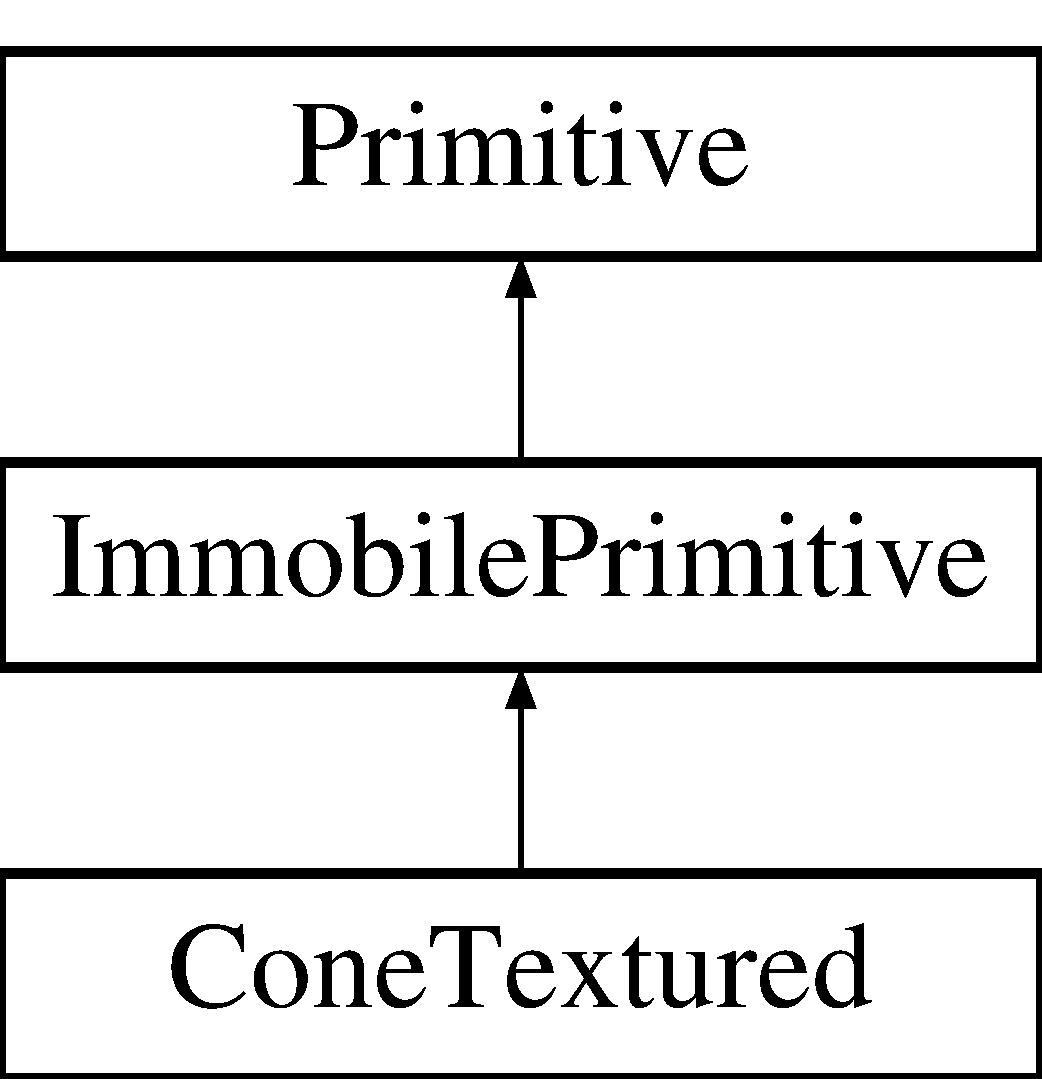
\includegraphics[height=3.000000cm]{class_cone_textured}
\end{center}
\end{figure}
\subsection*{Public Member Functions}
\begin{DoxyCompactItemize}
\item 
\hyperlink{class_cone_textured_a4c8c4a32295527f54c8af0a64c552b56}{Cone\-Textured} (double radius, double height, double zoffset, int num\-Slices, int num\-Stacks, \hyperlink{class_texture}{Texture} $\ast$texture, double num\-Textures\-X, double num\-Textures\-Y)
\item 
\hyperlink{class_cone_textured_a1a98d084be791913ce93b02559aa85f8}{$\sim$\-Cone\-Textured} ()
\end{DoxyCompactItemize}
\subsection*{Additional Inherited Members}


\subsection{Constructor \& Destructor Documentation}
\hypertarget{class_cone_textured_a4c8c4a32295527f54c8af0a64c552b56}{\index{Cone\-Textured@{Cone\-Textured}!Cone\-Textured@{Cone\-Textured}}
\index{Cone\-Textured@{Cone\-Textured}!ConeTextured@{Cone\-Textured}}
\subsubsection[{Cone\-Textured}]{\setlength{\rightskip}{0pt plus 5cm}Cone\-Textured\-::\-Cone\-Textured (
\begin{DoxyParamCaption}
\item[{double}]{radius, }
\item[{double}]{height, }
\item[{double}]{zoffset, }
\item[{int}]{num\-Slices, }
\item[{int}]{num\-Stacks, }
\item[{{\bf Texture} $\ast$}]{texture, }
\item[{double}]{num\-Textures\-X, }
\item[{double}]{num\-Textures\-Y}
\end{DoxyParamCaption}
)}}\label{class_cone_textured_a4c8c4a32295527f54c8af0a64c552b56}
\hypertarget{class_cone_textured_a1a98d084be791913ce93b02559aa85f8}{\index{Cone\-Textured@{Cone\-Textured}!$\sim$\-Cone\-Textured@{$\sim$\-Cone\-Textured}}
\index{$\sim$\-Cone\-Textured@{$\sim$\-Cone\-Textured}!ConeTextured@{Cone\-Textured}}
\subsubsection[{$\sim$\-Cone\-Textured}]{\setlength{\rightskip}{0pt plus 5cm}Cone\-Textured\-::$\sim$\-Cone\-Textured (
\begin{DoxyParamCaption}
{}
\end{DoxyParamCaption}
)}}\label{class_cone_textured_a1a98d084be791913ce93b02559aa85f8}


The documentation for this class was generated from the following files\-:\begin{DoxyCompactItemize}
\item 
C\-:/\-Users/\-Owner/\-My Programming/\-Personal Projects/\-Video\-Games/\-Optimist Racing/src/\hyperlink{_primitive_8hpp}{Primitive.\-hpp}\item 
C\-:/\-Users/\-Owner/\-My Programming/\-Personal Projects/\-Video\-Games/\-Optimist Racing/src/\hyperlink{_primitive_8cpp}{Primitive.\-cpp}\end{DoxyCompactItemize}

\hypertarget{class_cylinder_textured}{\section{Cylinder\-Textured Class Reference}
\label{class_cylinder_textured}\index{Cylinder\-Textured@{Cylinder\-Textured}}
}


{\ttfamily \#include $<$Primitive.\-hpp$>$}

Inheritance diagram for Cylinder\-Textured\-:\begin{figure}[H]
\begin{center}
\leavevmode
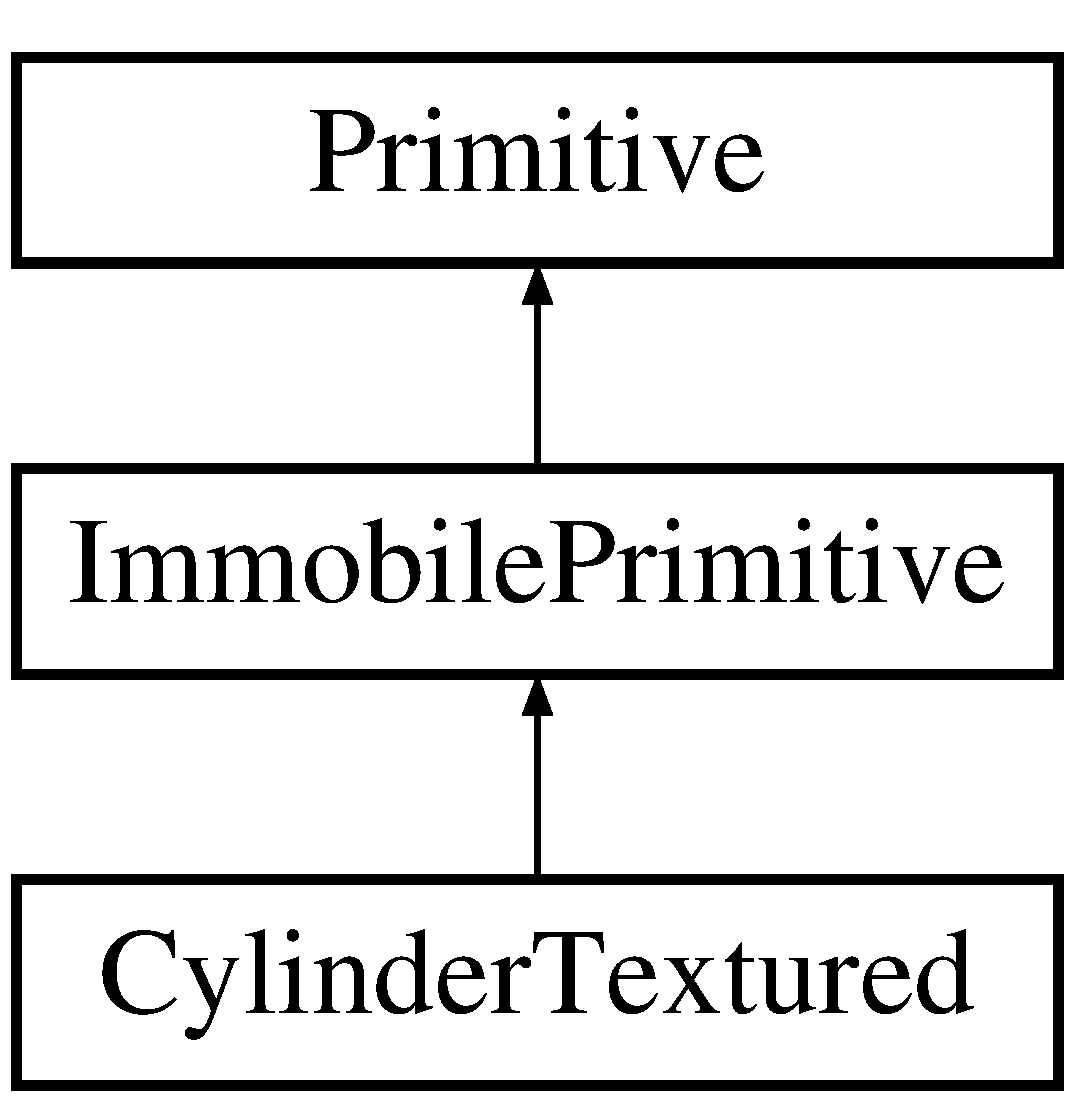
\includegraphics[height=3.000000cm]{class_cylinder_textured}
\end{center}
\end{figure}
\subsection*{Public Member Functions}
\begin{DoxyCompactItemize}
\item 
\hyperlink{class_cylinder_textured_a548d9c6be25c9fe1bcef06fdf69bfe5e}{Cylinder\-Textured} (double radius, double height, int num\-Quads, \hyperlink{class_texture}{Texture} $\ast$texture, double num\-Textures\-X, double num\-Textures\-Y)
\item 
\hyperlink{class_cylinder_textured_afce815dae7fb506d435d93adb35642bd}{$\sim$\-Cylinder\-Textured} ()
\end{DoxyCompactItemize}
\subsection*{Additional Inherited Members}


\subsection{Constructor \& Destructor Documentation}
\hypertarget{class_cylinder_textured_a548d9c6be25c9fe1bcef06fdf69bfe5e}{\index{Cylinder\-Textured@{Cylinder\-Textured}!Cylinder\-Textured@{Cylinder\-Textured}}
\index{Cylinder\-Textured@{Cylinder\-Textured}!CylinderTextured@{Cylinder\-Textured}}
\subsubsection[{Cylinder\-Textured}]{\setlength{\rightskip}{0pt plus 5cm}Cylinder\-Textured\-::\-Cylinder\-Textured (
\begin{DoxyParamCaption}
\item[{double}]{radius, }
\item[{double}]{height, }
\item[{int}]{num\-Quads, }
\item[{{\bf Texture} $\ast$}]{texture, }
\item[{double}]{num\-Textures\-X, }
\item[{double}]{num\-Textures\-Y}
\end{DoxyParamCaption}
)}}\label{class_cylinder_textured_a548d9c6be25c9fe1bcef06fdf69bfe5e}
\hypertarget{class_cylinder_textured_afce815dae7fb506d435d93adb35642bd}{\index{Cylinder\-Textured@{Cylinder\-Textured}!$\sim$\-Cylinder\-Textured@{$\sim$\-Cylinder\-Textured}}
\index{$\sim$\-Cylinder\-Textured@{$\sim$\-Cylinder\-Textured}!CylinderTextured@{Cylinder\-Textured}}
\subsubsection[{$\sim$\-Cylinder\-Textured}]{\setlength{\rightskip}{0pt plus 5cm}Cylinder\-Textured\-::$\sim$\-Cylinder\-Textured (
\begin{DoxyParamCaption}
{}
\end{DoxyParamCaption}
)}}\label{class_cylinder_textured_afce815dae7fb506d435d93adb35642bd}


The documentation for this class was generated from the following files\-:\begin{DoxyCompactItemize}
\item 
C\-:/\-Users/\-Owner/\-My Programming/\-Personal Projects/\-Video\-Games/\-Optimist Racing/src/\hyperlink{_primitive_8hpp}{Primitive.\-hpp}\item 
C\-:/\-Users/\-Owner/\-My Programming/\-Personal Projects/\-Video\-Games/\-Optimist Racing/src/\hyperlink{_primitive_8cpp}{Primitive.\-cpp}\end{DoxyCompactItemize}

\hypertarget{class_electric_material_data}{\section{Electric\-Material\-Data Class Reference}
\label{class_electric_material_data}\index{Electric\-Material\-Data@{Electric\-Material\-Data}}
}


{\ttfamily \#include $<$Data.\-hpp$>$}

Inheritance diagram for Electric\-Material\-Data\-:\begin{figure}[H]
\begin{center}
\leavevmode
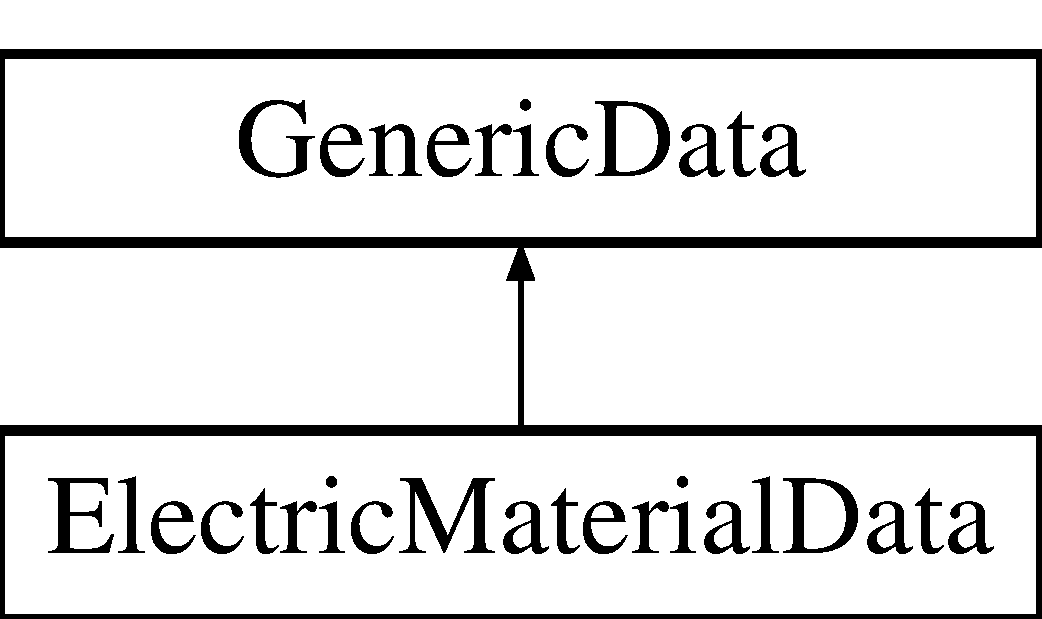
\includegraphics[height=2.000000cm]{class_electric_material_data}
\end{center}
\end{figure}
\subsection*{Public Member Functions}
\begin{DoxyCompactItemize}
\item 
\hyperlink{class_electric_material_data_afd70f2557397f9ba037ccb7e29610928}{Electric\-Material\-Data} (std\-::string filename)
\item 
\hyperlink{class_electric_material_data_a8f9dcfc5028fdcc9cc0cab2cefc5d8a4}{Electric\-Material\-Data} ()
\item 
\hyperlink{class_electric_material_data_a6ca55be54566379286b4dae00a2bc9f3}{$\sim$\-Electric\-Material\-Data} ()
\item 
\hyperlink{class_material}{Material} $\ast$$\ast$ \hyperlink{class_electric_material_data_a461c256f5e82c54b68c9ca51bed0fa4a}{create8\-Materials} ()
\item 
virtual void \hyperlink{class_electric_material_data_a81244b200484e145a684c56e6f9f1252}{write} (std\-::ostream \&out) const 
\item 
virtual void \hyperlink{class_electric_material_data_ab63a0313df28615504c4a7c57adef637}{read} (std\-::istream \&in)
\end{DoxyCompactItemize}
\subsection*{Public Attributes}
\begin{DoxyCompactItemize}
\item 
double \hyperlink{class_electric_material_data_ad0b9e1983b34e1995d0c662007b5b773}{m\-Emission\-On}
\item 
double \hyperlink{class_electric_material_data_a7463eb3c1e7839a5be7afca67191e405}{m\-Emission\-Off}
\item 
double \hyperlink{class_electric_material_data_a5251ccabe0243a8c8a783c1e105bd151}{m\-Ambient\-On}
\item 
double \hyperlink{class_electric_material_data_ac403298c9ad462c7722aa6ecf5078a26}{m\-Ambient\-Off}
\item 
double \hyperlink{class_electric_material_data_a142f858836d56cdfd13eff14aaea6e89}{m\-Diffuse\-On}
\item 
double \hyperlink{class_electric_material_data_ae26b6c78ca76ba31c349a8c17fc44989}{m\-Diffuse\-Off}
\item 
double \hyperlink{class_electric_material_data_a57d818c17fc37e8e44871f1310d84a1c}{m\-Specular\-On}
\item 
double \hyperlink{class_electric_material_data_aba5b236744527ecb0c3a391967b87575}{m\-Specular\-Off}
\item 
double \hyperlink{class_electric_material_data_aa6e7cc7da2cece949af3e9907eeaf98d}{m\-Shininess}
\end{DoxyCompactItemize}


\subsection{Constructor \& Destructor Documentation}
\hypertarget{class_electric_material_data_afd70f2557397f9ba037ccb7e29610928}{\index{Electric\-Material\-Data@{Electric\-Material\-Data}!Electric\-Material\-Data@{Electric\-Material\-Data}}
\index{Electric\-Material\-Data@{Electric\-Material\-Data}!ElectricMaterialData@{Electric\-Material\-Data}}
\subsubsection[{Electric\-Material\-Data}]{\setlength{\rightskip}{0pt plus 5cm}Electric\-Material\-Data\-::\-Electric\-Material\-Data (
\begin{DoxyParamCaption}
\item[{std\-::string}]{filename}
\end{DoxyParamCaption}
)}}\label{class_electric_material_data_afd70f2557397f9ba037ccb7e29610928}
\hypertarget{class_electric_material_data_a8f9dcfc5028fdcc9cc0cab2cefc5d8a4}{\index{Electric\-Material\-Data@{Electric\-Material\-Data}!Electric\-Material\-Data@{Electric\-Material\-Data}}
\index{Electric\-Material\-Data@{Electric\-Material\-Data}!ElectricMaterialData@{Electric\-Material\-Data}}
\subsubsection[{Electric\-Material\-Data}]{\setlength{\rightskip}{0pt plus 5cm}Electric\-Material\-Data\-::\-Electric\-Material\-Data (
\begin{DoxyParamCaption}
{}
\end{DoxyParamCaption}
)}}\label{class_electric_material_data_a8f9dcfc5028fdcc9cc0cab2cefc5d8a4}
\hypertarget{class_electric_material_data_a6ca55be54566379286b4dae00a2bc9f3}{\index{Electric\-Material\-Data@{Electric\-Material\-Data}!$\sim$\-Electric\-Material\-Data@{$\sim$\-Electric\-Material\-Data}}
\index{$\sim$\-Electric\-Material\-Data@{$\sim$\-Electric\-Material\-Data}!ElectricMaterialData@{Electric\-Material\-Data}}
\subsubsection[{$\sim$\-Electric\-Material\-Data}]{\setlength{\rightskip}{0pt plus 5cm}Electric\-Material\-Data\-::$\sim$\-Electric\-Material\-Data (
\begin{DoxyParamCaption}
{}
\end{DoxyParamCaption}
)}}\label{class_electric_material_data_a6ca55be54566379286b4dae00a2bc9f3}


\subsection{Member Function Documentation}
\hypertarget{class_electric_material_data_a461c256f5e82c54b68c9ca51bed0fa4a}{\index{Electric\-Material\-Data@{Electric\-Material\-Data}!create8\-Materials@{create8\-Materials}}
\index{create8\-Materials@{create8\-Materials}!ElectricMaterialData@{Electric\-Material\-Data}}
\subsubsection[{create8\-Materials}]{\setlength{\rightskip}{0pt plus 5cm}{\bf Material} $\ast$$\ast$ Electric\-Material\-Data\-::create8\-Materials (
\begin{DoxyParamCaption}
{}
\end{DoxyParamCaption}
)}}\label{class_electric_material_data_a461c256f5e82c54b68c9ca51bed0fa4a}
\hypertarget{class_electric_material_data_ab63a0313df28615504c4a7c57adef637}{\index{Electric\-Material\-Data@{Electric\-Material\-Data}!read@{read}}
\index{read@{read}!ElectricMaterialData@{Electric\-Material\-Data}}
\subsubsection[{read}]{\setlength{\rightskip}{0pt plus 5cm}void Electric\-Material\-Data\-::read (
\begin{DoxyParamCaption}
\item[{std\-::istream \&}]{in}
\end{DoxyParamCaption}
)\hspace{0.3cm}{\ttfamily [virtual]}}}\label{class_electric_material_data_ab63a0313df28615504c4a7c57adef637}


Implements \hyperlink{class_generic_data_a71e231ef04c9a91a3429123dab5bd1e7}{Generic\-Data}.

\hypertarget{class_electric_material_data_a81244b200484e145a684c56e6f9f1252}{\index{Electric\-Material\-Data@{Electric\-Material\-Data}!write@{write}}
\index{write@{write}!ElectricMaterialData@{Electric\-Material\-Data}}
\subsubsection[{write}]{\setlength{\rightskip}{0pt plus 5cm}void Electric\-Material\-Data\-::write (
\begin{DoxyParamCaption}
\item[{std\-::ostream \&}]{out}
\end{DoxyParamCaption}
) const\hspace{0.3cm}{\ttfamily [virtual]}}}\label{class_electric_material_data_a81244b200484e145a684c56e6f9f1252}


Implements \hyperlink{class_generic_data_a93ea61de5b09cf3fc95564ef3d841214}{Generic\-Data}.



\subsection{Member Data Documentation}
\hypertarget{class_electric_material_data_ac403298c9ad462c7722aa6ecf5078a26}{\index{Electric\-Material\-Data@{Electric\-Material\-Data}!m\-Ambient\-Off@{m\-Ambient\-Off}}
\index{m\-Ambient\-Off@{m\-Ambient\-Off}!ElectricMaterialData@{Electric\-Material\-Data}}
\subsubsection[{m\-Ambient\-Off}]{\setlength{\rightskip}{0pt plus 5cm}double Electric\-Material\-Data\-::m\-Ambient\-Off}}\label{class_electric_material_data_ac403298c9ad462c7722aa6ecf5078a26}
\hypertarget{class_electric_material_data_a5251ccabe0243a8c8a783c1e105bd151}{\index{Electric\-Material\-Data@{Electric\-Material\-Data}!m\-Ambient\-On@{m\-Ambient\-On}}
\index{m\-Ambient\-On@{m\-Ambient\-On}!ElectricMaterialData@{Electric\-Material\-Data}}
\subsubsection[{m\-Ambient\-On}]{\setlength{\rightskip}{0pt plus 5cm}double Electric\-Material\-Data\-::m\-Ambient\-On}}\label{class_electric_material_data_a5251ccabe0243a8c8a783c1e105bd151}
\hypertarget{class_electric_material_data_ae26b6c78ca76ba31c349a8c17fc44989}{\index{Electric\-Material\-Data@{Electric\-Material\-Data}!m\-Diffuse\-Off@{m\-Diffuse\-Off}}
\index{m\-Diffuse\-Off@{m\-Diffuse\-Off}!ElectricMaterialData@{Electric\-Material\-Data}}
\subsubsection[{m\-Diffuse\-Off}]{\setlength{\rightskip}{0pt plus 5cm}double Electric\-Material\-Data\-::m\-Diffuse\-Off}}\label{class_electric_material_data_ae26b6c78ca76ba31c349a8c17fc44989}
\hypertarget{class_electric_material_data_a142f858836d56cdfd13eff14aaea6e89}{\index{Electric\-Material\-Data@{Electric\-Material\-Data}!m\-Diffuse\-On@{m\-Diffuse\-On}}
\index{m\-Diffuse\-On@{m\-Diffuse\-On}!ElectricMaterialData@{Electric\-Material\-Data}}
\subsubsection[{m\-Diffuse\-On}]{\setlength{\rightskip}{0pt plus 5cm}double Electric\-Material\-Data\-::m\-Diffuse\-On}}\label{class_electric_material_data_a142f858836d56cdfd13eff14aaea6e89}
\hypertarget{class_electric_material_data_a7463eb3c1e7839a5be7afca67191e405}{\index{Electric\-Material\-Data@{Electric\-Material\-Data}!m\-Emission\-Off@{m\-Emission\-Off}}
\index{m\-Emission\-Off@{m\-Emission\-Off}!ElectricMaterialData@{Electric\-Material\-Data}}
\subsubsection[{m\-Emission\-Off}]{\setlength{\rightskip}{0pt plus 5cm}double Electric\-Material\-Data\-::m\-Emission\-Off}}\label{class_electric_material_data_a7463eb3c1e7839a5be7afca67191e405}
\hypertarget{class_electric_material_data_ad0b9e1983b34e1995d0c662007b5b773}{\index{Electric\-Material\-Data@{Electric\-Material\-Data}!m\-Emission\-On@{m\-Emission\-On}}
\index{m\-Emission\-On@{m\-Emission\-On}!ElectricMaterialData@{Electric\-Material\-Data}}
\subsubsection[{m\-Emission\-On}]{\setlength{\rightskip}{0pt plus 5cm}double Electric\-Material\-Data\-::m\-Emission\-On}}\label{class_electric_material_data_ad0b9e1983b34e1995d0c662007b5b773}
\hypertarget{class_electric_material_data_aa6e7cc7da2cece949af3e9907eeaf98d}{\index{Electric\-Material\-Data@{Electric\-Material\-Data}!m\-Shininess@{m\-Shininess}}
\index{m\-Shininess@{m\-Shininess}!ElectricMaterialData@{Electric\-Material\-Data}}
\subsubsection[{m\-Shininess}]{\setlength{\rightskip}{0pt plus 5cm}double Electric\-Material\-Data\-::m\-Shininess}}\label{class_electric_material_data_aa6e7cc7da2cece949af3e9907eeaf98d}
\hypertarget{class_electric_material_data_aba5b236744527ecb0c3a391967b87575}{\index{Electric\-Material\-Data@{Electric\-Material\-Data}!m\-Specular\-Off@{m\-Specular\-Off}}
\index{m\-Specular\-Off@{m\-Specular\-Off}!ElectricMaterialData@{Electric\-Material\-Data}}
\subsubsection[{m\-Specular\-Off}]{\setlength{\rightskip}{0pt plus 5cm}double Electric\-Material\-Data\-::m\-Specular\-Off}}\label{class_electric_material_data_aba5b236744527ecb0c3a391967b87575}
\hypertarget{class_electric_material_data_a57d818c17fc37e8e44871f1310d84a1c}{\index{Electric\-Material\-Data@{Electric\-Material\-Data}!m\-Specular\-On@{m\-Specular\-On}}
\index{m\-Specular\-On@{m\-Specular\-On}!ElectricMaterialData@{Electric\-Material\-Data}}
\subsubsection[{m\-Specular\-On}]{\setlength{\rightskip}{0pt plus 5cm}double Electric\-Material\-Data\-::m\-Specular\-On}}\label{class_electric_material_data_a57d818c17fc37e8e44871f1310d84a1c}


The documentation for this class was generated from the following files\-:\begin{DoxyCompactItemize}
\item 
C\-:/\-Users/\-Owner/\-My Programming/\-Personal Projects/\-Video\-Games/\-Optimist Racing/src/\hyperlink{_data_8hpp}{Data.\-hpp}\item 
C\-:/\-Users/\-Owner/\-My Programming/\-Personal Projects/\-Video\-Games/\-Optimist Racing/src/\hyperlink{_data_8cpp}{Data.\-cpp}\end{DoxyCompactItemize}

\hypertarget{class_floor_data}{\section{Floor\-Data Class Reference}
\label{class_floor_data}\index{Floor\-Data@{Floor\-Data}}
}


{\ttfamily \#include $<$Data.\-hpp$>$}

Inheritance diagram for Floor\-Data\-:\begin{figure}[H]
\begin{center}
\leavevmode
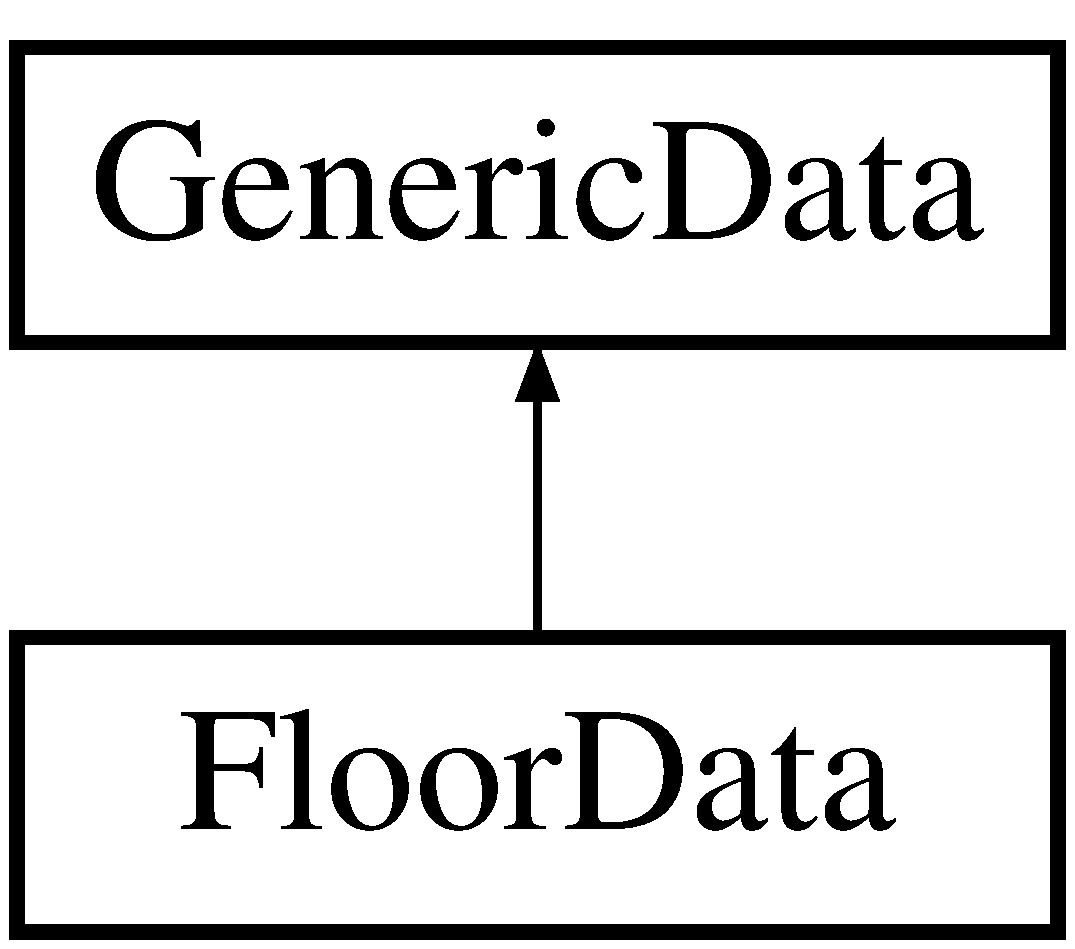
\includegraphics[height=2.000000cm]{class_floor_data}
\end{center}
\end{figure}
\subsection*{Public Member Functions}
\begin{DoxyCompactItemize}
\item 
\hyperlink{class_floor_data_a44d58e5e0b7461808ba4103b3a104cbe}{Floor\-Data} (std\-::string filename)
\item 
\hyperlink{class_floor_data_a3d165cd27d2deb6fc8b6a6f02f74f935}{Floor\-Data} ()
\item 
\hyperlink{class_floor_data_a2559119f4344bb8d8bed6e1f8d3c2813}{$\sim$\-Floor\-Data} ()
\item 
void \hyperlink{class_floor_data_a444c2b30a5e13fea21ce81b8deb9d14d}{initialize\-Default} ()
\item 
void \hyperlink{class_floor_data_aaee4c2e3e72268a529b162d29a98dcaf}{delete\-Arrays} ()
\item 
virtual void \hyperlink{class_floor_data_acbd1e6dfa4e2112d1e53c1dfd0703ee4}{write} (std\-::ostream \&out) const 
\item 
virtual void \hyperlink{class_floor_data_a137a204c7e37ac44eb721e984b5dad4c}{read} (std\-::istream \&in)
\end{DoxyCompactItemize}
\subsection*{Public Attributes}
\begin{DoxyCompactItemize}
\item 
double \hyperlink{class_floor_data_a38eed166299a5c25dd4358964afa0a2a}{m\-Floor\-Bezier\-H\-X}
\item 
double \hyperlink{class_floor_data_a264969dc13604a1a021e4b7084c2c00a}{m\-Floor\-Bezier\-H\-Y}
\item 
int \hyperlink{class_floor_data_a01fcc4a53643be6819fc3a8488436135}{m\-Floor\-Bezier\-Num\-Cells\-X}
\item 
int \hyperlink{class_floor_data_a79cc90d0b076ef2a7204d3f16480f1d5}{m\-Floor\-Bezier\-Num\-Cells\-Y}
\item 
\hyperlink{class_matrix_mx_n}{Matrix\-Mx\-N} $\ast$$\ast$ \hyperlink{class_floor_data_aef2684a379485861a0b2f81fe62df2df}{m\-Floor\-Bezier\-Fs}
\item 
\hyperlink{_electric_colour_8hpp_a1979e84576b59c4d100d8a8cc41de734}{E\-\_\-\-E\-L\-E\-C\-T\-R\-I\-C\-C\-O\-L\-O\-U\-R} $\ast$ \hyperlink{class_floor_data_aaf030f1c62c18bde64f0dbf3f6d08242}{m\-Floor\-Colours}
\end{DoxyCompactItemize}


\subsection{Constructor \& Destructor Documentation}
\hypertarget{class_floor_data_a44d58e5e0b7461808ba4103b3a104cbe}{\index{Floor\-Data@{Floor\-Data}!Floor\-Data@{Floor\-Data}}
\index{Floor\-Data@{Floor\-Data}!FloorData@{Floor\-Data}}
\subsubsection[{Floor\-Data}]{\setlength{\rightskip}{0pt plus 5cm}Floor\-Data\-::\-Floor\-Data (
\begin{DoxyParamCaption}
\item[{std\-::string}]{filename}
\end{DoxyParamCaption}
)}}\label{class_floor_data_a44d58e5e0b7461808ba4103b3a104cbe}
\hypertarget{class_floor_data_a3d165cd27d2deb6fc8b6a6f02f74f935}{\index{Floor\-Data@{Floor\-Data}!Floor\-Data@{Floor\-Data}}
\index{Floor\-Data@{Floor\-Data}!FloorData@{Floor\-Data}}
\subsubsection[{Floor\-Data}]{\setlength{\rightskip}{0pt plus 5cm}Floor\-Data\-::\-Floor\-Data (
\begin{DoxyParamCaption}
{}
\end{DoxyParamCaption}
)}}\label{class_floor_data_a3d165cd27d2deb6fc8b6a6f02f74f935}
\hypertarget{class_floor_data_a2559119f4344bb8d8bed6e1f8d3c2813}{\index{Floor\-Data@{Floor\-Data}!$\sim$\-Floor\-Data@{$\sim$\-Floor\-Data}}
\index{$\sim$\-Floor\-Data@{$\sim$\-Floor\-Data}!FloorData@{Floor\-Data}}
\subsubsection[{$\sim$\-Floor\-Data}]{\setlength{\rightskip}{0pt plus 5cm}Floor\-Data\-::$\sim$\-Floor\-Data (
\begin{DoxyParamCaption}
{}
\end{DoxyParamCaption}
)}}\label{class_floor_data_a2559119f4344bb8d8bed6e1f8d3c2813}


\subsection{Member Function Documentation}
\hypertarget{class_floor_data_aaee4c2e3e72268a529b162d29a98dcaf}{\index{Floor\-Data@{Floor\-Data}!delete\-Arrays@{delete\-Arrays}}
\index{delete\-Arrays@{delete\-Arrays}!FloorData@{Floor\-Data}}
\subsubsection[{delete\-Arrays}]{\setlength{\rightskip}{0pt plus 5cm}void Floor\-Data\-::delete\-Arrays (
\begin{DoxyParamCaption}
{}
\end{DoxyParamCaption}
)}}\label{class_floor_data_aaee4c2e3e72268a529b162d29a98dcaf}
\hypertarget{class_floor_data_a444c2b30a5e13fea21ce81b8deb9d14d}{\index{Floor\-Data@{Floor\-Data}!initialize\-Default@{initialize\-Default}}
\index{initialize\-Default@{initialize\-Default}!FloorData@{Floor\-Data}}
\subsubsection[{initialize\-Default}]{\setlength{\rightskip}{0pt plus 5cm}void Floor\-Data\-::initialize\-Default (
\begin{DoxyParamCaption}
{}
\end{DoxyParamCaption}
)}}\label{class_floor_data_a444c2b30a5e13fea21ce81b8deb9d14d}
\hypertarget{class_floor_data_a137a204c7e37ac44eb721e984b5dad4c}{\index{Floor\-Data@{Floor\-Data}!read@{read}}
\index{read@{read}!FloorData@{Floor\-Data}}
\subsubsection[{read}]{\setlength{\rightskip}{0pt plus 5cm}void Floor\-Data\-::read (
\begin{DoxyParamCaption}
\item[{std\-::istream \&}]{in}
\end{DoxyParamCaption}
)\hspace{0.3cm}{\ttfamily [virtual]}}}\label{class_floor_data_a137a204c7e37ac44eb721e984b5dad4c}


Implements \hyperlink{class_generic_data_a71e231ef04c9a91a3429123dab5bd1e7}{Generic\-Data}.

\hypertarget{class_floor_data_acbd1e6dfa4e2112d1e53c1dfd0703ee4}{\index{Floor\-Data@{Floor\-Data}!write@{write}}
\index{write@{write}!FloorData@{Floor\-Data}}
\subsubsection[{write}]{\setlength{\rightskip}{0pt plus 5cm}void Floor\-Data\-::write (
\begin{DoxyParamCaption}
\item[{std\-::ostream \&}]{out}
\end{DoxyParamCaption}
) const\hspace{0.3cm}{\ttfamily [virtual]}}}\label{class_floor_data_acbd1e6dfa4e2112d1e53c1dfd0703ee4}


Implements \hyperlink{class_generic_data_a93ea61de5b09cf3fc95564ef3d841214}{Generic\-Data}.



\subsection{Member Data Documentation}
\hypertarget{class_floor_data_aef2684a379485861a0b2f81fe62df2df}{\index{Floor\-Data@{Floor\-Data}!m\-Floor\-Bezier\-Fs@{m\-Floor\-Bezier\-Fs}}
\index{m\-Floor\-Bezier\-Fs@{m\-Floor\-Bezier\-Fs}!FloorData@{Floor\-Data}}
\subsubsection[{m\-Floor\-Bezier\-Fs}]{\setlength{\rightskip}{0pt plus 5cm}{\bf Matrix\-Mx\-N}$\ast$$\ast$ Floor\-Data\-::m\-Floor\-Bezier\-Fs}}\label{class_floor_data_aef2684a379485861a0b2f81fe62df2df}
\hypertarget{class_floor_data_a38eed166299a5c25dd4358964afa0a2a}{\index{Floor\-Data@{Floor\-Data}!m\-Floor\-Bezier\-H\-X@{m\-Floor\-Bezier\-H\-X}}
\index{m\-Floor\-Bezier\-H\-X@{m\-Floor\-Bezier\-H\-X}!FloorData@{Floor\-Data}}
\subsubsection[{m\-Floor\-Bezier\-H\-X}]{\setlength{\rightskip}{0pt plus 5cm}double Floor\-Data\-::m\-Floor\-Bezier\-H\-X}}\label{class_floor_data_a38eed166299a5c25dd4358964afa0a2a}
\hypertarget{class_floor_data_a264969dc13604a1a021e4b7084c2c00a}{\index{Floor\-Data@{Floor\-Data}!m\-Floor\-Bezier\-H\-Y@{m\-Floor\-Bezier\-H\-Y}}
\index{m\-Floor\-Bezier\-H\-Y@{m\-Floor\-Bezier\-H\-Y}!FloorData@{Floor\-Data}}
\subsubsection[{m\-Floor\-Bezier\-H\-Y}]{\setlength{\rightskip}{0pt plus 5cm}double Floor\-Data\-::m\-Floor\-Bezier\-H\-Y}}\label{class_floor_data_a264969dc13604a1a021e4b7084c2c00a}
\hypertarget{class_floor_data_a01fcc4a53643be6819fc3a8488436135}{\index{Floor\-Data@{Floor\-Data}!m\-Floor\-Bezier\-Num\-Cells\-X@{m\-Floor\-Bezier\-Num\-Cells\-X}}
\index{m\-Floor\-Bezier\-Num\-Cells\-X@{m\-Floor\-Bezier\-Num\-Cells\-X}!FloorData@{Floor\-Data}}
\subsubsection[{m\-Floor\-Bezier\-Num\-Cells\-X}]{\setlength{\rightskip}{0pt plus 5cm}int Floor\-Data\-::m\-Floor\-Bezier\-Num\-Cells\-X}}\label{class_floor_data_a01fcc4a53643be6819fc3a8488436135}
\hypertarget{class_floor_data_a79cc90d0b076ef2a7204d3f16480f1d5}{\index{Floor\-Data@{Floor\-Data}!m\-Floor\-Bezier\-Num\-Cells\-Y@{m\-Floor\-Bezier\-Num\-Cells\-Y}}
\index{m\-Floor\-Bezier\-Num\-Cells\-Y@{m\-Floor\-Bezier\-Num\-Cells\-Y}!FloorData@{Floor\-Data}}
\subsubsection[{m\-Floor\-Bezier\-Num\-Cells\-Y}]{\setlength{\rightskip}{0pt plus 5cm}int Floor\-Data\-::m\-Floor\-Bezier\-Num\-Cells\-Y}}\label{class_floor_data_a79cc90d0b076ef2a7204d3f16480f1d5}
\hypertarget{class_floor_data_aaf030f1c62c18bde64f0dbf3f6d08242}{\index{Floor\-Data@{Floor\-Data}!m\-Floor\-Colours@{m\-Floor\-Colours}}
\index{m\-Floor\-Colours@{m\-Floor\-Colours}!FloorData@{Floor\-Data}}
\subsubsection[{m\-Floor\-Colours}]{\setlength{\rightskip}{0pt plus 5cm}{\bf E\-\_\-\-E\-L\-E\-C\-T\-R\-I\-C\-C\-O\-L\-O\-U\-R}$\ast$ Floor\-Data\-::m\-Floor\-Colours}}\label{class_floor_data_aaf030f1c62c18bde64f0dbf3f6d08242}


The documentation for this class was generated from the following files\-:\begin{DoxyCompactItemize}
\item 
C\-:/\-Users/\-Owner/\-My Programming/\-Personal Projects/\-Video\-Games/\-Optimist Racing/src/\hyperlink{_data_8hpp}{Data.\-hpp}\item 
C\-:/\-Users/\-Owner/\-My Programming/\-Personal Projects/\-Video\-Games/\-Optimist Racing/src/\hyperlink{_data_8cpp}{Data.\-cpp}\end{DoxyCompactItemize}

\hypertarget{class_floor_render_data}{\section{Floor\-Render\-Data Class Reference}
\label{class_floor_render_data}\index{Floor\-Render\-Data@{Floor\-Render\-Data}}
}


{\ttfamily \#include $<$Data.\-hpp$>$}

Inheritance diagram for Floor\-Render\-Data\-:\begin{figure}[H]
\begin{center}
\leavevmode
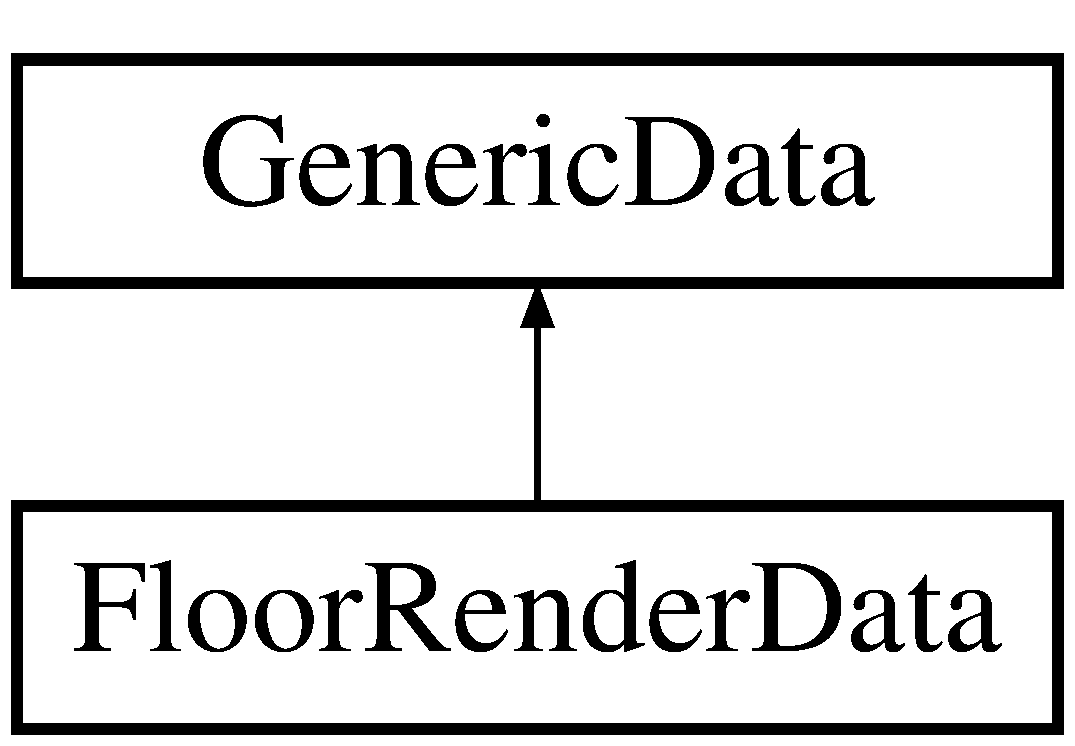
\includegraphics[height=2.000000cm]{class_floor_render_data}
\end{center}
\end{figure}
\subsection*{Public Member Functions}
\begin{DoxyCompactItemize}
\item 
\hyperlink{class_floor_render_data_ad40ad1c8a5c3cbf74cf154c4075e675a}{Floor\-Render\-Data} (std\-::string filename)
\item 
\hyperlink{class_floor_render_data_a784aafb1ab4f32823b0f6cc439e90bbb}{Floor\-Render\-Data} ()
\item 
\hyperlink{class_floor_render_data_aeaedcca3caa68ac4c23f5eb653b2c839}{$\sim$\-Floor\-Render\-Data} ()
\item 
virtual void \hyperlink{class_floor_render_data_a0303743e7939b4cf8bd9c155b79c07f3}{write} (std\-::ostream \&out) const 
\item 
virtual void \hyperlink{class_floor_render_data_a781daa3645a4924dc9f5df99a0c28b67}{read} (std\-::istream \&in)
\end{DoxyCompactItemize}
\subsection*{Public Attributes}
\begin{DoxyCompactItemize}
\item 
int \hyperlink{class_floor_render_data_af2f9d563314481158845495692fe31e7}{m\-Floor\-Render\-Cells\-Per\-Patch\-X}
\item 
int \hyperlink{class_floor_render_data_a1a563fff5b57ea69ba9bb192873c09db}{m\-Floor\-Render\-Cells\-Per\-Patch\-Y}
\item 
std\-::string \hyperlink{class_floor_render_data_ac1540b554998d32dabc4d69af1e92f0d}{m\-Floor\-Render\-Texture\-Filename}
\item 
double \hyperlink{class_floor_render_data_a7135effa977d515b9d3b648531b0b730}{m\-Floor\-Render\-Textures\-Per\-Patch\-X}
\item 
double \hyperlink{class_floor_render_data_afc74644c8e0c98fadcb158a5e3cd7e10}{m\-Floor\-Render\-Textures\-Per\-Patch\-Y}
\item 
\hyperlink{class_electric_material_data}{Electric\-Material\-Data} \hyperlink{class_floor_render_data_a58cca19207e9f58aabde32f83267e918}{m\-Floor\-Material}
\end{DoxyCompactItemize}


\subsection{Constructor \& Destructor Documentation}
\hypertarget{class_floor_render_data_ad40ad1c8a5c3cbf74cf154c4075e675a}{\index{Floor\-Render\-Data@{Floor\-Render\-Data}!Floor\-Render\-Data@{Floor\-Render\-Data}}
\index{Floor\-Render\-Data@{Floor\-Render\-Data}!FloorRenderData@{Floor\-Render\-Data}}
\subsubsection[{Floor\-Render\-Data}]{\setlength{\rightskip}{0pt plus 5cm}Floor\-Render\-Data\-::\-Floor\-Render\-Data (
\begin{DoxyParamCaption}
\item[{std\-::string}]{filename}
\end{DoxyParamCaption}
)}}\label{class_floor_render_data_ad40ad1c8a5c3cbf74cf154c4075e675a}
\hypertarget{class_floor_render_data_a784aafb1ab4f32823b0f6cc439e90bbb}{\index{Floor\-Render\-Data@{Floor\-Render\-Data}!Floor\-Render\-Data@{Floor\-Render\-Data}}
\index{Floor\-Render\-Data@{Floor\-Render\-Data}!FloorRenderData@{Floor\-Render\-Data}}
\subsubsection[{Floor\-Render\-Data}]{\setlength{\rightskip}{0pt plus 5cm}Floor\-Render\-Data\-::\-Floor\-Render\-Data (
\begin{DoxyParamCaption}
{}
\end{DoxyParamCaption}
)}}\label{class_floor_render_data_a784aafb1ab4f32823b0f6cc439e90bbb}
\hypertarget{class_floor_render_data_aeaedcca3caa68ac4c23f5eb653b2c839}{\index{Floor\-Render\-Data@{Floor\-Render\-Data}!$\sim$\-Floor\-Render\-Data@{$\sim$\-Floor\-Render\-Data}}
\index{$\sim$\-Floor\-Render\-Data@{$\sim$\-Floor\-Render\-Data}!FloorRenderData@{Floor\-Render\-Data}}
\subsubsection[{$\sim$\-Floor\-Render\-Data}]{\setlength{\rightskip}{0pt plus 5cm}Floor\-Render\-Data\-::$\sim$\-Floor\-Render\-Data (
\begin{DoxyParamCaption}
{}
\end{DoxyParamCaption}
)}}\label{class_floor_render_data_aeaedcca3caa68ac4c23f5eb653b2c839}


\subsection{Member Function Documentation}
\hypertarget{class_floor_render_data_a781daa3645a4924dc9f5df99a0c28b67}{\index{Floor\-Render\-Data@{Floor\-Render\-Data}!read@{read}}
\index{read@{read}!FloorRenderData@{Floor\-Render\-Data}}
\subsubsection[{read}]{\setlength{\rightskip}{0pt plus 5cm}void Floor\-Render\-Data\-::read (
\begin{DoxyParamCaption}
\item[{std\-::istream \&}]{in}
\end{DoxyParamCaption}
)\hspace{0.3cm}{\ttfamily [virtual]}}}\label{class_floor_render_data_a781daa3645a4924dc9f5df99a0c28b67}


Implements \hyperlink{class_generic_data_a71e231ef04c9a91a3429123dab5bd1e7}{Generic\-Data}.

\hypertarget{class_floor_render_data_a0303743e7939b4cf8bd9c155b79c07f3}{\index{Floor\-Render\-Data@{Floor\-Render\-Data}!write@{write}}
\index{write@{write}!FloorRenderData@{Floor\-Render\-Data}}
\subsubsection[{write}]{\setlength{\rightskip}{0pt plus 5cm}void Floor\-Render\-Data\-::write (
\begin{DoxyParamCaption}
\item[{std\-::ostream \&}]{out}
\end{DoxyParamCaption}
) const\hspace{0.3cm}{\ttfamily [virtual]}}}\label{class_floor_render_data_a0303743e7939b4cf8bd9c155b79c07f3}


Implements \hyperlink{class_generic_data_a93ea61de5b09cf3fc95564ef3d841214}{Generic\-Data}.



\subsection{Member Data Documentation}
\hypertarget{class_floor_render_data_a58cca19207e9f58aabde32f83267e918}{\index{Floor\-Render\-Data@{Floor\-Render\-Data}!m\-Floor\-Material@{m\-Floor\-Material}}
\index{m\-Floor\-Material@{m\-Floor\-Material}!FloorRenderData@{Floor\-Render\-Data}}
\subsubsection[{m\-Floor\-Material}]{\setlength{\rightskip}{0pt plus 5cm}{\bf Electric\-Material\-Data} Floor\-Render\-Data\-::m\-Floor\-Material}}\label{class_floor_render_data_a58cca19207e9f58aabde32f83267e918}
\hypertarget{class_floor_render_data_af2f9d563314481158845495692fe31e7}{\index{Floor\-Render\-Data@{Floor\-Render\-Data}!m\-Floor\-Render\-Cells\-Per\-Patch\-X@{m\-Floor\-Render\-Cells\-Per\-Patch\-X}}
\index{m\-Floor\-Render\-Cells\-Per\-Patch\-X@{m\-Floor\-Render\-Cells\-Per\-Patch\-X}!FloorRenderData@{Floor\-Render\-Data}}
\subsubsection[{m\-Floor\-Render\-Cells\-Per\-Patch\-X}]{\setlength{\rightskip}{0pt plus 5cm}int Floor\-Render\-Data\-::m\-Floor\-Render\-Cells\-Per\-Patch\-X}}\label{class_floor_render_data_af2f9d563314481158845495692fe31e7}
\hypertarget{class_floor_render_data_a1a563fff5b57ea69ba9bb192873c09db}{\index{Floor\-Render\-Data@{Floor\-Render\-Data}!m\-Floor\-Render\-Cells\-Per\-Patch\-Y@{m\-Floor\-Render\-Cells\-Per\-Patch\-Y}}
\index{m\-Floor\-Render\-Cells\-Per\-Patch\-Y@{m\-Floor\-Render\-Cells\-Per\-Patch\-Y}!FloorRenderData@{Floor\-Render\-Data}}
\subsubsection[{m\-Floor\-Render\-Cells\-Per\-Patch\-Y}]{\setlength{\rightskip}{0pt plus 5cm}int Floor\-Render\-Data\-::m\-Floor\-Render\-Cells\-Per\-Patch\-Y}}\label{class_floor_render_data_a1a563fff5b57ea69ba9bb192873c09db}
\hypertarget{class_floor_render_data_ac1540b554998d32dabc4d69af1e92f0d}{\index{Floor\-Render\-Data@{Floor\-Render\-Data}!m\-Floor\-Render\-Texture\-Filename@{m\-Floor\-Render\-Texture\-Filename}}
\index{m\-Floor\-Render\-Texture\-Filename@{m\-Floor\-Render\-Texture\-Filename}!FloorRenderData@{Floor\-Render\-Data}}
\subsubsection[{m\-Floor\-Render\-Texture\-Filename}]{\setlength{\rightskip}{0pt plus 5cm}std\-::string Floor\-Render\-Data\-::m\-Floor\-Render\-Texture\-Filename}}\label{class_floor_render_data_ac1540b554998d32dabc4d69af1e92f0d}
\hypertarget{class_floor_render_data_a7135effa977d515b9d3b648531b0b730}{\index{Floor\-Render\-Data@{Floor\-Render\-Data}!m\-Floor\-Render\-Textures\-Per\-Patch\-X@{m\-Floor\-Render\-Textures\-Per\-Patch\-X}}
\index{m\-Floor\-Render\-Textures\-Per\-Patch\-X@{m\-Floor\-Render\-Textures\-Per\-Patch\-X}!FloorRenderData@{Floor\-Render\-Data}}
\subsubsection[{m\-Floor\-Render\-Textures\-Per\-Patch\-X}]{\setlength{\rightskip}{0pt plus 5cm}double Floor\-Render\-Data\-::m\-Floor\-Render\-Textures\-Per\-Patch\-X}}\label{class_floor_render_data_a7135effa977d515b9d3b648531b0b730}
\hypertarget{class_floor_render_data_afc74644c8e0c98fadcb158a5e3cd7e10}{\index{Floor\-Render\-Data@{Floor\-Render\-Data}!m\-Floor\-Render\-Textures\-Per\-Patch\-Y@{m\-Floor\-Render\-Textures\-Per\-Patch\-Y}}
\index{m\-Floor\-Render\-Textures\-Per\-Patch\-Y@{m\-Floor\-Render\-Textures\-Per\-Patch\-Y}!FloorRenderData@{Floor\-Render\-Data}}
\subsubsection[{m\-Floor\-Render\-Textures\-Per\-Patch\-Y}]{\setlength{\rightskip}{0pt plus 5cm}double Floor\-Render\-Data\-::m\-Floor\-Render\-Textures\-Per\-Patch\-Y}}\label{class_floor_render_data_afc74644c8e0c98fadcb158a5e3cd7e10}


The documentation for this class was generated from the following files\-:\begin{DoxyCompactItemize}
\item 
C\-:/\-Users/\-Owner/\-My Programming/\-Personal Projects/\-Video\-Games/\-Optimist Racing/src/\hyperlink{_data_8hpp}{Data.\-hpp}\item 
C\-:/\-Users/\-Owner/\-My Programming/\-Personal Projects/\-Video\-Games/\-Optimist Racing/src/\hyperlink{_data_8cpp}{Data.\-cpp}\end{DoxyCompactItemize}

\hypertarget{class_generic_data}{\section{Generic\-Data Class Reference}
\label{class_generic_data}\index{Generic\-Data@{Generic\-Data}}
}


{\ttfamily \#include $<$Data.\-hpp$>$}

Inheritance diagram for Generic\-Data\-:\begin{figure}[H]
\begin{center}
\leavevmode
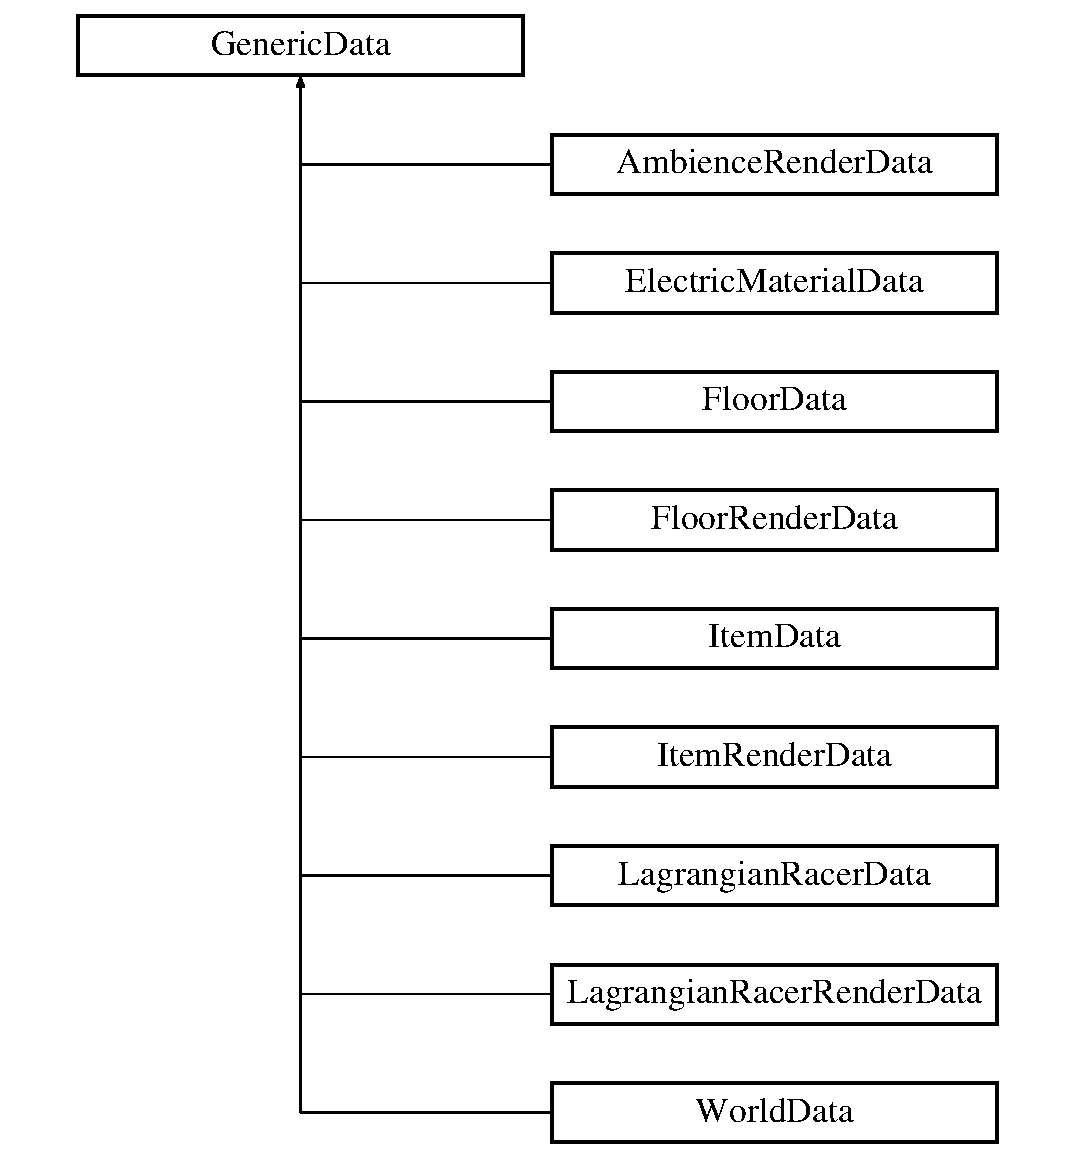
\includegraphics[height=10.000000cm]{class_generic_data}
\end{center}
\end{figure}
\subsection*{Public Member Functions}
\begin{DoxyCompactItemize}
\item 
\hyperlink{class_generic_data_a53d266970be68cd208cabbf1b029b96b}{Generic\-Data} ()
\item 
\hyperlink{class_generic_data_a9ab691aa9487309b2c4d9f5a0be19464}{$\sim$\-Generic\-Data} ()
\item 
virtual void \hyperlink{class_generic_data_a93ea61de5b09cf3fc95564ef3d841214}{write} (std\-::ostream \&out) const =0
\item 
virtual void \hyperlink{class_generic_data_a71e231ef04c9a91a3429123dab5bd1e7}{read} (std\-::istream \&in)=0
\item 
void \hyperlink{class_generic_data_ab2b2fb8564b784d61b99ab4f7fd95dc2}{write\-File} (const std\-::string filepath) const 
\item 
void \hyperlink{class_generic_data_a7d833405e216a292dc0655692df370e1}{read\-File} (const std\-::string filepath)
\end{DoxyCompactItemize}


\subsection{Constructor \& Destructor Documentation}
\hypertarget{class_generic_data_a53d266970be68cd208cabbf1b029b96b}{\index{Generic\-Data@{Generic\-Data}!Generic\-Data@{Generic\-Data}}
\index{Generic\-Data@{Generic\-Data}!GenericData@{Generic\-Data}}
\subsubsection[{Generic\-Data}]{\setlength{\rightskip}{0pt plus 5cm}Generic\-Data\-::\-Generic\-Data (
\begin{DoxyParamCaption}
{}
\end{DoxyParamCaption}
)\hspace{0.3cm}{\ttfamily [inline]}}}\label{class_generic_data_a53d266970be68cd208cabbf1b029b96b}
\hypertarget{class_generic_data_a9ab691aa9487309b2c4d9f5a0be19464}{\index{Generic\-Data@{Generic\-Data}!$\sim$\-Generic\-Data@{$\sim$\-Generic\-Data}}
\index{$\sim$\-Generic\-Data@{$\sim$\-Generic\-Data}!GenericData@{Generic\-Data}}
\subsubsection[{$\sim$\-Generic\-Data}]{\setlength{\rightskip}{0pt plus 5cm}Generic\-Data\-::$\sim$\-Generic\-Data (
\begin{DoxyParamCaption}
{}
\end{DoxyParamCaption}
)\hspace{0.3cm}{\ttfamily [inline]}}}\label{class_generic_data_a9ab691aa9487309b2c4d9f5a0be19464}


\subsection{Member Function Documentation}
\hypertarget{class_generic_data_a71e231ef04c9a91a3429123dab5bd1e7}{\index{Generic\-Data@{Generic\-Data}!read@{read}}
\index{read@{read}!GenericData@{Generic\-Data}}
\subsubsection[{read}]{\setlength{\rightskip}{0pt plus 5cm}virtual void Generic\-Data\-::read (
\begin{DoxyParamCaption}
\item[{std\-::istream \&}]{in}
\end{DoxyParamCaption}
)\hspace{0.3cm}{\ttfamily [pure virtual]}}}\label{class_generic_data_a71e231ef04c9a91a3429123dab5bd1e7}


Implemented in \hyperlink{class_world_data_aa80956a9e1337417f570f776edeb1c5e}{World\-Data}, \hyperlink{class_item_render_data_afbda96d49108440c6ce4a9c0b541116f}{Item\-Render\-Data}, \hyperlink{class_item_data_a71b90a70f427ee1d2417f3f0c7302c9e}{Item\-Data}, \hyperlink{class_ambience_render_data_a051acf84a9c31c6e439e7d7e7445ef47}{Ambience\-Render\-Data}, \hyperlink{class_lagrangian_racer_render_data_aa5174615686e62f00cf5d71ff870e5ca}{Lagrangian\-Racer\-Render\-Data}, \hyperlink{class_lagrangian_racer_data_a5985c44e28872d0064596a3104f2feff}{Lagrangian\-Racer\-Data}, \hyperlink{class_floor_render_data_a781daa3645a4924dc9f5df99a0c28b67}{Floor\-Render\-Data}, \hyperlink{class_floor_data_a137a204c7e37ac44eb721e984b5dad4c}{Floor\-Data}, and \hyperlink{class_electric_material_data_ab63a0313df28615504c4a7c57adef637}{Electric\-Material\-Data}.

\hypertarget{class_generic_data_a7d833405e216a292dc0655692df370e1}{\index{Generic\-Data@{Generic\-Data}!read\-File@{read\-File}}
\index{read\-File@{read\-File}!GenericData@{Generic\-Data}}
\subsubsection[{read\-File}]{\setlength{\rightskip}{0pt plus 5cm}void Generic\-Data\-::read\-File (
\begin{DoxyParamCaption}
\item[{const std\-::string}]{filepath}
\end{DoxyParamCaption}
)}}\label{class_generic_data_a7d833405e216a292dc0655692df370e1}
\hypertarget{class_generic_data_a93ea61de5b09cf3fc95564ef3d841214}{\index{Generic\-Data@{Generic\-Data}!write@{write}}
\index{write@{write}!GenericData@{Generic\-Data}}
\subsubsection[{write}]{\setlength{\rightskip}{0pt plus 5cm}virtual void Generic\-Data\-::write (
\begin{DoxyParamCaption}
\item[{std\-::ostream \&}]{out}
\end{DoxyParamCaption}
) const\hspace{0.3cm}{\ttfamily [pure virtual]}}}\label{class_generic_data_a93ea61de5b09cf3fc95564ef3d841214}


Implemented in \hyperlink{class_world_data_aa8a0d950e6d52f7c7baebb722804f55d}{World\-Data}, \hyperlink{class_item_render_data_a13f92fc9e5386ef04fb736fbacc17a7e}{Item\-Render\-Data}, \hyperlink{class_item_data_aff74199fbef4ff9f8b06c186173e69ea}{Item\-Data}, \hyperlink{class_ambience_render_data_a04e058a2c8b174def8c381a19ede0d12}{Ambience\-Render\-Data}, \hyperlink{class_lagrangian_racer_render_data_a5df4617924f398cd1bf7c0fd633e8020}{Lagrangian\-Racer\-Render\-Data}, \hyperlink{class_lagrangian_racer_data_adbea50ddbb24883866bb828985fa6164}{Lagrangian\-Racer\-Data}, \hyperlink{class_floor_render_data_a0303743e7939b4cf8bd9c155b79c07f3}{Floor\-Render\-Data}, \hyperlink{class_floor_data_acbd1e6dfa4e2112d1e53c1dfd0703ee4}{Floor\-Data}, and \hyperlink{class_electric_material_data_a81244b200484e145a684c56e6f9f1252}{Electric\-Material\-Data}.

\hypertarget{class_generic_data_ab2b2fb8564b784d61b99ab4f7fd95dc2}{\index{Generic\-Data@{Generic\-Data}!write\-File@{write\-File}}
\index{write\-File@{write\-File}!GenericData@{Generic\-Data}}
\subsubsection[{write\-File}]{\setlength{\rightskip}{0pt plus 5cm}void Generic\-Data\-::write\-File (
\begin{DoxyParamCaption}
\item[{const std\-::string}]{filepath}
\end{DoxyParamCaption}
) const}}\label{class_generic_data_ab2b2fb8564b784d61b99ab4f7fd95dc2}


The documentation for this class was generated from the following files\-:\begin{DoxyCompactItemize}
\item 
C\-:/\-Users/\-Owner/\-My Programming/\-Personal Projects/\-Video\-Games/\-Optimist Racing/src/\hyperlink{_data_8hpp}{Data.\-hpp}\item 
C\-:/\-Users/\-Owner/\-My Programming/\-Personal Projects/\-Video\-Games/\-Optimist Racing/src/\hyperlink{_data_8cpp}{Data.\-cpp}\end{DoxyCompactItemize}

\hypertarget{class_grid2_d}{\section{Grid2\-D$<$ T $>$ Class Template Reference}
\label{class_grid2_d}\index{Grid2\-D$<$ T $>$@{Grid2\-D$<$ T $>$}}
}


A 2d grid where each cell has a value.  




{\ttfamily \#include $<$Grid.\-hpp$>$}

\subsection*{Public Member Functions}
\begin{DoxyCompactItemize}
\item 
\hyperlink{class_grid2_d_a2d0de43afc44cfa9b1f85e2a89407987}{Grid2\-D} (double origin\-X, double origin\-Y, int num\-Cells\-X, int num\-Cells\-Y, double grid\-H\-X, double grid\-H\-Y, T $\ast$values)
\begin{DoxyCompactList}\small\item\em Basic constructor. \end{DoxyCompactList}\item 
\hyperlink{class_grid2_d_a882eef0c27a9c0dc379254633f6b4632}{$\sim$\-Grid2\-D} ()
\begin{DoxyCompactList}\small\item\em The destructor. \end{DoxyCompactList}\item 
double \hyperlink{class_grid2_d_a297945ebee6053b879eb2302fb997257}{get\-Origin\-X} () const 
\begin{DoxyCompactList}\small\item\em Returns the x-\/value of the origin of the grid (bottom-\/left corner). \end{DoxyCompactList}\item 
double \hyperlink{class_grid2_d_ae84fe7442dccef0d49eedc65fe96b06a}{get\-Origin\-Y} () const 
\begin{DoxyCompactList}\small\item\em Returns the y-\/value of the origin of the grid (bottom-\/left corner). \end{DoxyCompactList}\item 
double \hyperlink{class_grid2_d_a93655a3d92f6f98eeb6ec5826cd89249}{get\-Grid\-H\-X} () const 
\begin{DoxyCompactList}\small\item\em Returns the x-\/spacing of the grid (the width of each cell). \end{DoxyCompactList}\item 
double \hyperlink{class_grid2_d_a23b8af0f8e33c530bd1afbc5c77c50e2}{get\-Grid\-H\-Y} () const 
\begin{DoxyCompactList}\small\item\em Returns the y-\/spacing of the grid (the height of each cell). \end{DoxyCompactList}\item 
int \hyperlink{class_grid2_d_a2b6c57bd0364ec5ec86ac5adf84bcbc5}{get\-Num\-Cells\-X} () const 
\begin{DoxyCompactList}\small\item\em Returns the number of cells across the x-\/direction. \end{DoxyCompactList}\item 
int \hyperlink{class_grid2_d_aaa3fd3dbe8e175ae01bf51af3dac72bc}{get\-Num\-Cells\-Y} () const 
\begin{DoxyCompactList}\small\item\em Returns the number of cells across the y-\/direction. \end{DoxyCompactList}\item 
T \hyperlink{class_grid2_d_a35171b27de35bf8ea47437e35a06ada7}{get\-Value} (int i, int j, T default\-Value) const 
\begin{DoxyCompactList}\small\item\em Returns the value at the cell number \mbox{[}i,j\mbox{]}. \end{DoxyCompactList}\item 
T \hyperlink{class_grid2_d_aa40e58a8322d1abf80f7479cc86f7dda}{get\-Value} (double x, double y, T default\-Value) const 
\begin{DoxyCompactList}\small\item\em Returns the value at the point (x,y) (takes into account grid spacing). \end{DoxyCompactList}\end{DoxyCompactItemize}


\subsection{Detailed Description}
\subsubsection*{template$<$typename T$>$class Grid2\-D$<$ T $>$}

A 2d grid where each cell has a value. 

Represents a 2d grid with constant spacing (may be different for x and y) where each cell has a value. \begin{DoxyAuthor}{Author}
Claude Richard 
\end{DoxyAuthor}
\begin{DoxyDate}{Date}
2012 
\end{DoxyDate}


\subsection{Constructor \& Destructor Documentation}
\hypertarget{class_grid2_d_a2d0de43afc44cfa9b1f85e2a89407987}{\index{Grid2\-D@{Grid2\-D}!Grid2\-D@{Grid2\-D}}
\index{Grid2\-D@{Grid2\-D}!Grid2D@{Grid2\-D}}
\subsubsection[{Grid2\-D}]{\setlength{\rightskip}{0pt plus 5cm}template$<$typename T$>$ {\bf Grid2\-D}$<$ T $>$\-::{\bf Grid2\-D} (
\begin{DoxyParamCaption}
\item[{double}]{origin\-X, }
\item[{double}]{origin\-Y, }
\item[{int}]{num\-Cells\-X, }
\item[{int}]{num\-Cells\-Y, }
\item[{double}]{grid\-H\-X, }
\item[{double}]{grid\-H\-Y, }
\item[{T $\ast$}]{values}
\end{DoxyParamCaption}
)\hspace{0.3cm}{\ttfamily [inline]}}}\label{class_grid2_d_a2d0de43afc44cfa9b1f85e2a89407987}


Basic constructor. 

In this constructor, everything about the grid is specified in the arguments. \begin{DoxyPrecond}{Precondition}
The values in the {\itshape values} array must be ordered as follows\-: (x1,y1), (x2,y1), (x3,y1), ... , (xm,yn). 
\end{DoxyPrecond}
\begin{DoxyPostcond}{Postcondition}
This object will represent a 2d grid, with origin (origin\-X,origin\-Y), x-\/spacing grid\-H\-X, y-\/spacing grid\-H\-Y, with num\-Cells\-X cells along the x-\/axis and num\-Cells\-Y cells along the y-\/axis. The origin is the bottom-\/left corner of the grid. This object will not hold a pointer to {\itshape values}; it simply copies the array. 
\end{DoxyPostcond}

\begin{DoxyParams}{Parameters}
{\em origin\-X} & The origin's x-\/value, which is the smallest x-\/value on the grid. \\
\hline
{\em origin\-Y} & The origin's y-\/value, which is the smallest y-\/value on the grid. \\
\hline
{\em num\-Cells\-X} & The number of cells counting along the x-\/axis. \\
\hline
{\em num\-Cells\-Y} & The number of cells counting along the y-\/axis. \\
\hline
\end{DoxyParams}

\begin{DoxyExceptions}{Exceptions}
{\em An} & error if {\itshape values} has length smaller than {\itshape num\-Cells\-X} $\ast$ {\itshape num\-Cells\-Y}. An error if any of grid\-H\-X, grid\-H\-Y, num\-Cells\-X, or num\-Cells\-Y is $<$= 0. \\
\hline
\end{DoxyExceptions}
\hypertarget{class_grid2_d_a882eef0c27a9c0dc379254633f6b4632}{\index{Grid2\-D@{Grid2\-D}!$\sim$\-Grid2\-D@{$\sim$\-Grid2\-D}}
\index{$\sim$\-Grid2\-D@{$\sim$\-Grid2\-D}!Grid2D@{Grid2\-D}}
\subsubsection[{$\sim$\-Grid2\-D}]{\setlength{\rightskip}{0pt plus 5cm}template$<$typename T$>$ {\bf Grid2\-D}$<$ T $>$\-::$\sim${\bf Grid2\-D} (
\begin{DoxyParamCaption}
{}
\end{DoxyParamCaption}
)\hspace{0.3cm}{\ttfamily [inline]}}}\label{class_grid2_d_a882eef0c27a9c0dc379254633f6b4632}


The destructor. 

This destructor simply deletes its copy of the values array. 

\subsection{Member Function Documentation}
\hypertarget{class_grid2_d_a93655a3d92f6f98eeb6ec5826cd89249}{\index{Grid2\-D@{Grid2\-D}!get\-Grid\-H\-X@{get\-Grid\-H\-X}}
\index{get\-Grid\-H\-X@{get\-Grid\-H\-X}!Grid2D@{Grid2\-D}}
\subsubsection[{get\-Grid\-H\-X}]{\setlength{\rightskip}{0pt plus 5cm}template$<$typename T$>$ double {\bf Grid2\-D}$<$ T $>$\-::get\-Grid\-H\-X (
\begin{DoxyParamCaption}
{}
\end{DoxyParamCaption}
) const\hspace{0.3cm}{\ttfamily [inline]}}}\label{class_grid2_d_a93655a3d92f6f98eeb6ec5826cd89249}


Returns the x-\/spacing of the grid (the width of each cell). 

\begin{DoxyReturn}{Returns}
The x-\/spacing of the grid (the width of each cell). 
\end{DoxyReturn}
\hypertarget{class_grid2_d_a23b8af0f8e33c530bd1afbc5c77c50e2}{\index{Grid2\-D@{Grid2\-D}!get\-Grid\-H\-Y@{get\-Grid\-H\-Y}}
\index{get\-Grid\-H\-Y@{get\-Grid\-H\-Y}!Grid2D@{Grid2\-D}}
\subsubsection[{get\-Grid\-H\-Y}]{\setlength{\rightskip}{0pt plus 5cm}template$<$typename T$>$ double {\bf Grid2\-D}$<$ T $>$\-::get\-Grid\-H\-Y (
\begin{DoxyParamCaption}
{}
\end{DoxyParamCaption}
) const\hspace{0.3cm}{\ttfamily [inline]}}}\label{class_grid2_d_a23b8af0f8e33c530bd1afbc5c77c50e2}


Returns the y-\/spacing of the grid (the height of each cell). 

\begin{DoxyReturn}{Returns}
The y-\/spacing of the grid (the height of each cell). 
\end{DoxyReturn}
\hypertarget{class_grid2_d_a2b6c57bd0364ec5ec86ac5adf84bcbc5}{\index{Grid2\-D@{Grid2\-D}!get\-Num\-Cells\-X@{get\-Num\-Cells\-X}}
\index{get\-Num\-Cells\-X@{get\-Num\-Cells\-X}!Grid2D@{Grid2\-D}}
\subsubsection[{get\-Num\-Cells\-X}]{\setlength{\rightskip}{0pt plus 5cm}template$<$typename T$>$ int {\bf Grid2\-D}$<$ T $>$\-::get\-Num\-Cells\-X (
\begin{DoxyParamCaption}
{}
\end{DoxyParamCaption}
) const\hspace{0.3cm}{\ttfamily [inline]}}}\label{class_grid2_d_a2b6c57bd0364ec5ec86ac5adf84bcbc5}


Returns the number of cells across the x-\/direction. 

\begin{DoxyReturn}{Returns}
The number of cells across the x-\/direction. 
\end{DoxyReturn}
\hypertarget{class_grid2_d_aaa3fd3dbe8e175ae01bf51af3dac72bc}{\index{Grid2\-D@{Grid2\-D}!get\-Num\-Cells\-Y@{get\-Num\-Cells\-Y}}
\index{get\-Num\-Cells\-Y@{get\-Num\-Cells\-Y}!Grid2D@{Grid2\-D}}
\subsubsection[{get\-Num\-Cells\-Y}]{\setlength{\rightskip}{0pt plus 5cm}template$<$typename T$>$ int {\bf Grid2\-D}$<$ T $>$\-::get\-Num\-Cells\-Y (
\begin{DoxyParamCaption}
{}
\end{DoxyParamCaption}
) const\hspace{0.3cm}{\ttfamily [inline]}}}\label{class_grid2_d_aaa3fd3dbe8e175ae01bf51af3dac72bc}


Returns the number of cells across the y-\/direction. 

\begin{DoxyReturn}{Returns}
The number of cells across the y-\/direction. 
\end{DoxyReturn}
\hypertarget{class_grid2_d_a297945ebee6053b879eb2302fb997257}{\index{Grid2\-D@{Grid2\-D}!get\-Origin\-X@{get\-Origin\-X}}
\index{get\-Origin\-X@{get\-Origin\-X}!Grid2D@{Grid2\-D}}
\subsubsection[{get\-Origin\-X}]{\setlength{\rightskip}{0pt plus 5cm}template$<$typename T$>$ double {\bf Grid2\-D}$<$ T $>$\-::get\-Origin\-X (
\begin{DoxyParamCaption}
{}
\end{DoxyParamCaption}
) const\hspace{0.3cm}{\ttfamily [inline]}}}\label{class_grid2_d_a297945ebee6053b879eb2302fb997257}


Returns the x-\/value of the origin of the grid (bottom-\/left corner). 

\begin{DoxyReturn}{Returns}
The x-\/value of the origin of the grid (bottom-\/left corner). 
\end{DoxyReturn}
\hypertarget{class_grid2_d_ae84fe7442dccef0d49eedc65fe96b06a}{\index{Grid2\-D@{Grid2\-D}!get\-Origin\-Y@{get\-Origin\-Y}}
\index{get\-Origin\-Y@{get\-Origin\-Y}!Grid2D@{Grid2\-D}}
\subsubsection[{get\-Origin\-Y}]{\setlength{\rightskip}{0pt plus 5cm}template$<$typename T$>$ double {\bf Grid2\-D}$<$ T $>$\-::get\-Origin\-Y (
\begin{DoxyParamCaption}
{}
\end{DoxyParamCaption}
) const\hspace{0.3cm}{\ttfamily [inline]}}}\label{class_grid2_d_ae84fe7442dccef0d49eedc65fe96b06a}


Returns the y-\/value of the origin of the grid (bottom-\/left corner). 

\begin{DoxyReturn}{Returns}
The y-\/value of the origin of the grid (bottom-\/left corner). 
\end{DoxyReturn}
\hypertarget{class_grid2_d_a35171b27de35bf8ea47437e35a06ada7}{\index{Grid2\-D@{Grid2\-D}!get\-Value@{get\-Value}}
\index{get\-Value@{get\-Value}!Grid2D@{Grid2\-D}}
\subsubsection[{get\-Value}]{\setlength{\rightskip}{0pt plus 5cm}template$<$typename T$>$ T {\bf Grid2\-D}$<$ T $>$\-::get\-Value (
\begin{DoxyParamCaption}
\item[{int}]{i, }
\item[{int}]{j, }
\item[{T}]{default\-Value}
\end{DoxyParamCaption}
) const\hspace{0.3cm}{\ttfamily [inline]}}}\label{class_grid2_d_a35171b27de35bf8ea47437e35a06ada7}


Returns the value at the cell number \mbox{[}i,j\mbox{]}. 

If i or j is off the grid, then returns the value of the closest cell. 
\begin{DoxyParams}{Parameters}
{\em i} & The x-\/index of the cell (counting cells, not the x-\/value in the coordinate system). \\
\hline
{\em j} & The y-\/index of the cell (counting cells, not the y-\/value in the coordinate system). \\
\hline
{\em default\-Value} & The value to be returned if the cell-\/index \mbox{[}i,j\mbox{]} is outside the grid. \\
\hline
\end{DoxyParams}
\begin{DoxyReturn}{Returns}
The value at the cell number \mbox{[}i,j\mbox{]}. If i or j is off the grid, then returns {\itshape default\-Value}. 
\end{DoxyReturn}
\hypertarget{class_grid2_d_aa40e58a8322d1abf80f7479cc86f7dda}{\index{Grid2\-D@{Grid2\-D}!get\-Value@{get\-Value}}
\index{get\-Value@{get\-Value}!Grid2D@{Grid2\-D}}
\subsubsection[{get\-Value}]{\setlength{\rightskip}{0pt plus 5cm}template$<$typename T$>$ T {\bf Grid2\-D}$<$ T $>$\-::get\-Value (
\begin{DoxyParamCaption}
\item[{double}]{x, }
\item[{double}]{y, }
\item[{T}]{default\-Value}
\end{DoxyParamCaption}
) const\hspace{0.3cm}{\ttfamily [inline]}}}\label{class_grid2_d_aa40e58a8322d1abf80f7479cc86f7dda}


Returns the value at the point (x,y) (takes into account grid spacing). 

If (x,y) is off the grid, then returns {\itshape default\-Value}. 
\begin{DoxyParams}{Parameters}
{\em x} & The x-\/value of the point in the coordinate system. \\
\hline
{\em y} & The y-\/value of the point in the coordinate system. \\
\hline
{\em default\-Value} & The value to be returned if (x,y) is outside the grid. \\
\hline
\end{DoxyParams}
\begin{DoxyReturn}{Returns}
The value of the cell at (x,y). If (x,y) is off the grid, then returns {\itshape default\-Value}. 
\end{DoxyReturn}


The documentation for this class was generated from the following file\-:\begin{DoxyCompactItemize}
\item 
C\-:/\-Users/\-Owner/\-My Programming/\-Personal Projects/\-Video\-Games/\-Optimist Racing/src/\hyperlink{_grid_8hpp}{Grid.\-hpp}\end{DoxyCompactItemize}

\hypertarget{class_image}{\section{Image Class Reference}
\label{class_image}\index{Image@{Image}}
}


{\ttfamily \#include $<$Image.\-hpp$>$}

\subsection*{Public Member Functions}
\begin{DoxyCompactItemize}
\item 
\hyperlink{class_image_a58edd1c45b4faeb5f789b0d036d02313}{Image} ()
\item 
\hyperlink{class_image_a57fc741dbb4f5535564cecc08b48fbdc}{Image} (int num\-X, int num\-Y)
\item 
\hyperlink{class_image_afb1678cfc99d6e049769dec2ddff7e89}{Image} (int num\-X, int num\-Y, int num\-Colours)
\item 
\hyperlink{class_image_a0294f63700543e11c0f0da85601c7ae5}{$\sim$\-Image} ()
\item 
int \hyperlink{class_image_af2720a072812763395512fc3c8c21362}{get\-Width} ()
\item 
int \hyperlink{class_image_aa4e1f064e5e1f3f04ad605408f1ec3af}{get\-Height} ()
\item 
int \hyperlink{class_image_a8313a877af2a774dda00f99e4f2ff2d0}{get\-Num\-Colours} ()
\item 
int \hyperlink{class_image_a7e0accd8358ef5dc43d24f2f90941ced}{get\-Data} (int x, int y, int colour)
\item 
void \hyperlink{class_image_a3c6d45a4014645eafb25e09e3685f144}{read\-Png\-File} (const std\-::string \&filename)
\end{DoxyCompactItemize}


\subsection{Constructor \& Destructor Documentation}
\hypertarget{class_image_a58edd1c45b4faeb5f789b0d036d02313}{\index{Image@{Image}!Image@{Image}}
\index{Image@{Image}!Image@{Image}}
\subsubsection[{Image}]{\setlength{\rightskip}{0pt plus 5cm}Image\-::\-Image (
\begin{DoxyParamCaption}
{}
\end{DoxyParamCaption}
)}}\label{class_image_a58edd1c45b4faeb5f789b0d036d02313}
\hypertarget{class_image_a57fc741dbb4f5535564cecc08b48fbdc}{\index{Image@{Image}!Image@{Image}}
\index{Image@{Image}!Image@{Image}}
\subsubsection[{Image}]{\setlength{\rightskip}{0pt plus 5cm}Image\-::\-Image (
\begin{DoxyParamCaption}
\item[{int}]{num\-X, }
\item[{int}]{num\-Y}
\end{DoxyParamCaption}
)}}\label{class_image_a57fc741dbb4f5535564cecc08b48fbdc}
\hypertarget{class_image_afb1678cfc99d6e049769dec2ddff7e89}{\index{Image@{Image}!Image@{Image}}
\index{Image@{Image}!Image@{Image}}
\subsubsection[{Image}]{\setlength{\rightskip}{0pt plus 5cm}Image\-::\-Image (
\begin{DoxyParamCaption}
\item[{int}]{num\-X, }
\item[{int}]{num\-Y, }
\item[{int}]{num\-Colours}
\end{DoxyParamCaption}
)}}\label{class_image_afb1678cfc99d6e049769dec2ddff7e89}
\hypertarget{class_image_a0294f63700543e11c0f0da85601c7ae5}{\index{Image@{Image}!$\sim$\-Image@{$\sim$\-Image}}
\index{$\sim$\-Image@{$\sim$\-Image}!Image@{Image}}
\subsubsection[{$\sim$\-Image}]{\setlength{\rightskip}{0pt plus 5cm}Image\-::$\sim$\-Image (
\begin{DoxyParamCaption}
{}
\end{DoxyParamCaption}
)}}\label{class_image_a0294f63700543e11c0f0da85601c7ae5}


\subsection{Member Function Documentation}
\hypertarget{class_image_a7e0accd8358ef5dc43d24f2f90941ced}{\index{Image@{Image}!get\-Data@{get\-Data}}
\index{get\-Data@{get\-Data}!Image@{Image}}
\subsubsection[{get\-Data}]{\setlength{\rightskip}{0pt plus 5cm}int Image\-::get\-Data (
\begin{DoxyParamCaption}
\item[{int}]{x, }
\item[{int}]{y, }
\item[{int}]{colour}
\end{DoxyParamCaption}
)}}\label{class_image_a7e0accd8358ef5dc43d24f2f90941ced}
\hypertarget{class_image_aa4e1f064e5e1f3f04ad605408f1ec3af}{\index{Image@{Image}!get\-Height@{get\-Height}}
\index{get\-Height@{get\-Height}!Image@{Image}}
\subsubsection[{get\-Height}]{\setlength{\rightskip}{0pt plus 5cm}int Image\-::get\-Height (
\begin{DoxyParamCaption}
{}
\end{DoxyParamCaption}
)}}\label{class_image_aa4e1f064e5e1f3f04ad605408f1ec3af}
\hypertarget{class_image_a8313a877af2a774dda00f99e4f2ff2d0}{\index{Image@{Image}!get\-Num\-Colours@{get\-Num\-Colours}}
\index{get\-Num\-Colours@{get\-Num\-Colours}!Image@{Image}}
\subsubsection[{get\-Num\-Colours}]{\setlength{\rightskip}{0pt plus 5cm}int Image\-::get\-Num\-Colours (
\begin{DoxyParamCaption}
{}
\end{DoxyParamCaption}
)}}\label{class_image_a8313a877af2a774dda00f99e4f2ff2d0}
\hypertarget{class_image_af2720a072812763395512fc3c8c21362}{\index{Image@{Image}!get\-Width@{get\-Width}}
\index{get\-Width@{get\-Width}!Image@{Image}}
\subsubsection[{get\-Width}]{\setlength{\rightskip}{0pt plus 5cm}int Image\-::get\-Width (
\begin{DoxyParamCaption}
{}
\end{DoxyParamCaption}
)}}\label{class_image_af2720a072812763395512fc3c8c21362}
\hypertarget{class_image_a3c6d45a4014645eafb25e09e3685f144}{\index{Image@{Image}!read\-Png\-File@{read\-Png\-File}}
\index{read\-Png\-File@{read\-Png\-File}!Image@{Image}}
\subsubsection[{read\-Png\-File}]{\setlength{\rightskip}{0pt plus 5cm}void Image\-::read\-Png\-File (
\begin{DoxyParamCaption}
\item[{const std\-::string \&}]{filename}
\end{DoxyParamCaption}
)}}\label{class_image_a3c6d45a4014645eafb25e09e3685f144}


The documentation for this class was generated from the following files\-:\begin{DoxyCompactItemize}
\item 
C\-:/\-Users/\-Owner/\-My Programming/\-Personal Projects/\-Video\-Games/\-Optimist Racing/src/\hyperlink{_image_8hpp}{Image.\-hpp}\item 
C\-:/\-Users/\-Owner/\-My Programming/\-Personal Projects/\-Video\-Games/\-Optimist Racing/src/\hyperlink{_image_8cpp}{Image.\-cpp}\end{DoxyCompactItemize}

\hypertarget{class_immobile_primitive}{\section{Immobile\-Primitive Class Reference}
\label{class_immobile_primitive}\index{Immobile\-Primitive@{Immobile\-Primitive}}
}


{\ttfamily \#include $<$Primitive.\-hpp$>$}

Inheritance diagram for Immobile\-Primitive\-:\begin{figure}[H]
\begin{center}
\leavevmode
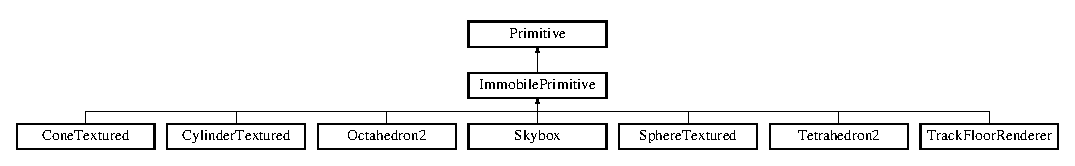
\includegraphics[height=1.777778cm]{class_immobile_primitive}
\end{center}
\end{figure}
\subsection*{Public Member Functions}
\begin{DoxyCompactItemize}
\item 
\hyperlink{class_immobile_primitive_a704ab830afc7d755d015977e30261355}{Immobile\-Primitive} ()
\item 
\hyperlink{class_immobile_primitive_a7d30116ce4bece945e95a5157ef053d8}{$\sim$\-Immobile\-Primitive} ()
\item 
void \hyperlink{class_immobile_primitive_ac6307f4bb055921e8727fd9a08d5dcce}{gl\-Render} () const 
\end{DoxyCompactItemize}
\subsection*{Protected Attributes}
\begin{DoxyCompactItemize}
\item 
G\-Luint \hyperlink{class_immobile_primitive_ae8a9856047b36aad734a887fc8361610}{m\-List}
\end{DoxyCompactItemize}
\subsection*{Additional Inherited Members}


\subsection{Constructor \& Destructor Documentation}
\hypertarget{class_immobile_primitive_a704ab830afc7d755d015977e30261355}{\index{Immobile\-Primitive@{Immobile\-Primitive}!Immobile\-Primitive@{Immobile\-Primitive}}
\index{Immobile\-Primitive@{Immobile\-Primitive}!ImmobilePrimitive@{Immobile\-Primitive}}
\subsubsection[{Immobile\-Primitive}]{\setlength{\rightskip}{0pt plus 5cm}Immobile\-Primitive\-::\-Immobile\-Primitive (
\begin{DoxyParamCaption}
{}
\end{DoxyParamCaption}
)}}\label{class_immobile_primitive_a704ab830afc7d755d015977e30261355}
\hypertarget{class_immobile_primitive_a7d30116ce4bece945e95a5157ef053d8}{\index{Immobile\-Primitive@{Immobile\-Primitive}!$\sim$\-Immobile\-Primitive@{$\sim$\-Immobile\-Primitive}}
\index{$\sim$\-Immobile\-Primitive@{$\sim$\-Immobile\-Primitive}!ImmobilePrimitive@{Immobile\-Primitive}}
\subsubsection[{$\sim$\-Immobile\-Primitive}]{\setlength{\rightskip}{0pt plus 5cm}Immobile\-Primitive\-::$\sim$\-Immobile\-Primitive (
\begin{DoxyParamCaption}
{}
\end{DoxyParamCaption}
)}}\label{class_immobile_primitive_a7d30116ce4bece945e95a5157ef053d8}


\subsection{Member Function Documentation}
\hypertarget{class_immobile_primitive_ac6307f4bb055921e8727fd9a08d5dcce}{\index{Immobile\-Primitive@{Immobile\-Primitive}!gl\-Render@{gl\-Render}}
\index{gl\-Render@{gl\-Render}!ImmobilePrimitive@{Immobile\-Primitive}}
\subsubsection[{gl\-Render}]{\setlength{\rightskip}{0pt plus 5cm}void Immobile\-Primitive\-::gl\-Render (
\begin{DoxyParamCaption}
{}
\end{DoxyParamCaption}
) const\hspace{0.3cm}{\ttfamily [virtual]}}}\label{class_immobile_primitive_ac6307f4bb055921e8727fd9a08d5dcce}


Implements \hyperlink{class_primitive_aef765029fae092f0f6dd1507e18e72e0}{Primitive}.



\subsection{Member Data Documentation}
\hypertarget{class_immobile_primitive_ae8a9856047b36aad734a887fc8361610}{\index{Immobile\-Primitive@{Immobile\-Primitive}!m\-List@{m\-List}}
\index{m\-List@{m\-List}!ImmobilePrimitive@{Immobile\-Primitive}}
\subsubsection[{m\-List}]{\setlength{\rightskip}{0pt plus 5cm}G\-Luint Immobile\-Primitive\-::m\-List\hspace{0.3cm}{\ttfamily [protected]}}}\label{class_immobile_primitive_ae8a9856047b36aad734a887fc8361610}


The documentation for this class was generated from the following files\-:\begin{DoxyCompactItemize}
\item 
C\-:/\-Users/\-Owner/\-My Programming/\-Personal Projects/\-Video\-Games/\-Optimist Racing/src/\hyperlink{_primitive_8hpp}{Primitive.\-hpp}\item 
C\-:/\-Users/\-Owner/\-My Programming/\-Personal Projects/\-Video\-Games/\-Optimist Racing/src/\hyperlink{_primitive_8cpp}{Primitive.\-cpp}\end{DoxyCompactItemize}

\hypertarget{class_item_data}{\section{Item\-Data Class Reference}
\label{class_item_data}\index{Item\-Data@{Item\-Data}}
}


{\ttfamily \#include $<$Data.\-hpp$>$}

Inheritance diagram for Item\-Data\-:\begin{figure}[H]
\begin{center}
\leavevmode
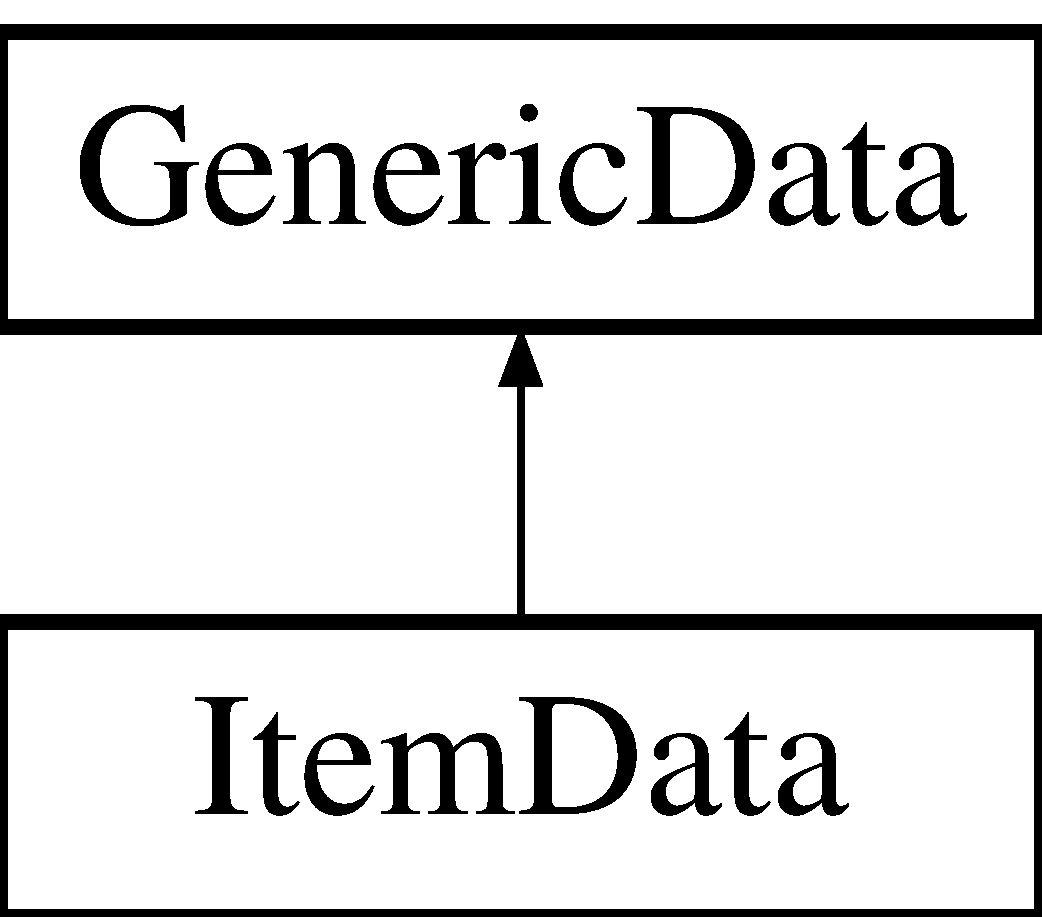
\includegraphics[height=2.000000cm]{class_item_data}
\end{center}
\end{figure}
\subsection*{Public Member Functions}
\begin{DoxyCompactItemize}
\item 
\hyperlink{class_item_data_a0e5968ac45fac4dee76ea9f75f7752cc}{Item\-Data} (std\-::string filename)
\item 
\hyperlink{class_item_data_a3a1b6240b016a82fa65b450f98a35f6c}{Item\-Data} ()
\item 
\hyperlink{class_item_data_ae155bfaeaa7badb8611595593d88f050}{$\sim$\-Item\-Data} ()
\item 
void \hyperlink{class_item_data_a7c0fd620ea4f6043558b80330f8bf51c}{initialize\-Default} ()
\item 
void \hyperlink{class_item_data_ab4cfa6f95e0662498d3df0f23c8127d4}{delete\-Arrays} ()
\item 
virtual void \hyperlink{class_item_data_aff74199fbef4ff9f8b06c186173e69ea}{write} (std\-::ostream \&out) const 
\item 
virtual void \hyperlink{class_item_data_a71b90a70f427ee1d2417f3f0c7302c9e}{read} (std\-::istream \&in)
\end{DoxyCompactItemize}
\subsection*{Public Attributes}
\begin{DoxyCompactItemize}
\item 
int \hyperlink{class_item_data_ad34492f2bef4ac472141c8c2f49a4453}{m\-Painter\-Num}
\item 
\hyperlink{class_vector3_d}{Vector3\-D} $\ast$ \hyperlink{class_item_data_a143e1354591086a1eccfa88a88142d80}{m\-Painter\-Positions}
\item 
\hyperlink{_electric_colour_8hpp_a1979e84576b59c4d100d8a8cc41de734}{E\-\_\-\-E\-L\-E\-C\-T\-R\-I\-C\-C\-O\-L\-O\-U\-R} $\ast$ \hyperlink{class_item_data_a96be973680b6a94519f07a7a660fd6f6}{m\-Painter\-Colours}
\item 
double \hyperlink{class_item_data_a44cc64e866c902fb5999e3169b440372}{m\-Painter\-Radius}
\item 
\hyperlink{class_vector3_d}{Vector3\-D} \hyperlink{class_item_data_a33649729ff05366dc714a903eafe7e47}{m\-End\-Position}
\item 
double \hyperlink{class_item_data_a0ba449b337e0596bd1401d6318cc1b8e}{m\-End\-Radius}
\end{DoxyCompactItemize}


\subsection{Constructor \& Destructor Documentation}
\hypertarget{class_item_data_a0e5968ac45fac4dee76ea9f75f7752cc}{\index{Item\-Data@{Item\-Data}!Item\-Data@{Item\-Data}}
\index{Item\-Data@{Item\-Data}!ItemData@{Item\-Data}}
\subsubsection[{Item\-Data}]{\setlength{\rightskip}{0pt plus 5cm}Item\-Data\-::\-Item\-Data (
\begin{DoxyParamCaption}
\item[{std\-::string}]{filename}
\end{DoxyParamCaption}
)}}\label{class_item_data_a0e5968ac45fac4dee76ea9f75f7752cc}
\hypertarget{class_item_data_a3a1b6240b016a82fa65b450f98a35f6c}{\index{Item\-Data@{Item\-Data}!Item\-Data@{Item\-Data}}
\index{Item\-Data@{Item\-Data}!ItemData@{Item\-Data}}
\subsubsection[{Item\-Data}]{\setlength{\rightskip}{0pt plus 5cm}Item\-Data\-::\-Item\-Data (
\begin{DoxyParamCaption}
{}
\end{DoxyParamCaption}
)}}\label{class_item_data_a3a1b6240b016a82fa65b450f98a35f6c}
\hypertarget{class_item_data_ae155bfaeaa7badb8611595593d88f050}{\index{Item\-Data@{Item\-Data}!$\sim$\-Item\-Data@{$\sim$\-Item\-Data}}
\index{$\sim$\-Item\-Data@{$\sim$\-Item\-Data}!ItemData@{Item\-Data}}
\subsubsection[{$\sim$\-Item\-Data}]{\setlength{\rightskip}{0pt plus 5cm}Item\-Data\-::$\sim$\-Item\-Data (
\begin{DoxyParamCaption}
{}
\end{DoxyParamCaption}
)}}\label{class_item_data_ae155bfaeaa7badb8611595593d88f050}


\subsection{Member Function Documentation}
\hypertarget{class_item_data_ab4cfa6f95e0662498d3df0f23c8127d4}{\index{Item\-Data@{Item\-Data}!delete\-Arrays@{delete\-Arrays}}
\index{delete\-Arrays@{delete\-Arrays}!ItemData@{Item\-Data}}
\subsubsection[{delete\-Arrays}]{\setlength{\rightskip}{0pt plus 5cm}void Item\-Data\-::delete\-Arrays (
\begin{DoxyParamCaption}
{}
\end{DoxyParamCaption}
)}}\label{class_item_data_ab4cfa6f95e0662498d3df0f23c8127d4}
\hypertarget{class_item_data_a7c0fd620ea4f6043558b80330f8bf51c}{\index{Item\-Data@{Item\-Data}!initialize\-Default@{initialize\-Default}}
\index{initialize\-Default@{initialize\-Default}!ItemData@{Item\-Data}}
\subsubsection[{initialize\-Default}]{\setlength{\rightskip}{0pt plus 5cm}void Item\-Data\-::initialize\-Default (
\begin{DoxyParamCaption}
{}
\end{DoxyParamCaption}
)}}\label{class_item_data_a7c0fd620ea4f6043558b80330f8bf51c}
\hypertarget{class_item_data_a71b90a70f427ee1d2417f3f0c7302c9e}{\index{Item\-Data@{Item\-Data}!read@{read}}
\index{read@{read}!ItemData@{Item\-Data}}
\subsubsection[{read}]{\setlength{\rightskip}{0pt plus 5cm}void Item\-Data\-::read (
\begin{DoxyParamCaption}
\item[{std\-::istream \&}]{in}
\end{DoxyParamCaption}
)\hspace{0.3cm}{\ttfamily [virtual]}}}\label{class_item_data_a71b90a70f427ee1d2417f3f0c7302c9e}


Implements \hyperlink{class_generic_data_a71e231ef04c9a91a3429123dab5bd1e7}{Generic\-Data}.

\hypertarget{class_item_data_aff74199fbef4ff9f8b06c186173e69ea}{\index{Item\-Data@{Item\-Data}!write@{write}}
\index{write@{write}!ItemData@{Item\-Data}}
\subsubsection[{write}]{\setlength{\rightskip}{0pt plus 5cm}void Item\-Data\-::write (
\begin{DoxyParamCaption}
\item[{std\-::ostream \&}]{out}
\end{DoxyParamCaption}
) const\hspace{0.3cm}{\ttfamily [virtual]}}}\label{class_item_data_aff74199fbef4ff9f8b06c186173e69ea}


Implements \hyperlink{class_generic_data_a93ea61de5b09cf3fc95564ef3d841214}{Generic\-Data}.



\subsection{Member Data Documentation}
\hypertarget{class_item_data_a33649729ff05366dc714a903eafe7e47}{\index{Item\-Data@{Item\-Data}!m\-End\-Position@{m\-End\-Position}}
\index{m\-End\-Position@{m\-End\-Position}!ItemData@{Item\-Data}}
\subsubsection[{m\-End\-Position}]{\setlength{\rightskip}{0pt plus 5cm}{\bf Vector3\-D} Item\-Data\-::m\-End\-Position}}\label{class_item_data_a33649729ff05366dc714a903eafe7e47}
\hypertarget{class_item_data_a0ba449b337e0596bd1401d6318cc1b8e}{\index{Item\-Data@{Item\-Data}!m\-End\-Radius@{m\-End\-Radius}}
\index{m\-End\-Radius@{m\-End\-Radius}!ItemData@{Item\-Data}}
\subsubsection[{m\-End\-Radius}]{\setlength{\rightskip}{0pt plus 5cm}double Item\-Data\-::m\-End\-Radius}}\label{class_item_data_a0ba449b337e0596bd1401d6318cc1b8e}
\hypertarget{class_item_data_a96be973680b6a94519f07a7a660fd6f6}{\index{Item\-Data@{Item\-Data}!m\-Painter\-Colours@{m\-Painter\-Colours}}
\index{m\-Painter\-Colours@{m\-Painter\-Colours}!ItemData@{Item\-Data}}
\subsubsection[{m\-Painter\-Colours}]{\setlength{\rightskip}{0pt plus 5cm}{\bf E\-\_\-\-E\-L\-E\-C\-T\-R\-I\-C\-C\-O\-L\-O\-U\-R}$\ast$ Item\-Data\-::m\-Painter\-Colours}}\label{class_item_data_a96be973680b6a94519f07a7a660fd6f6}
\hypertarget{class_item_data_ad34492f2bef4ac472141c8c2f49a4453}{\index{Item\-Data@{Item\-Data}!m\-Painter\-Num@{m\-Painter\-Num}}
\index{m\-Painter\-Num@{m\-Painter\-Num}!ItemData@{Item\-Data}}
\subsubsection[{m\-Painter\-Num}]{\setlength{\rightskip}{0pt plus 5cm}int Item\-Data\-::m\-Painter\-Num}}\label{class_item_data_ad34492f2bef4ac472141c8c2f49a4453}
\hypertarget{class_item_data_a143e1354591086a1eccfa88a88142d80}{\index{Item\-Data@{Item\-Data}!m\-Painter\-Positions@{m\-Painter\-Positions}}
\index{m\-Painter\-Positions@{m\-Painter\-Positions}!ItemData@{Item\-Data}}
\subsubsection[{m\-Painter\-Positions}]{\setlength{\rightskip}{0pt plus 5cm}{\bf Vector3\-D}$\ast$ Item\-Data\-::m\-Painter\-Positions}}\label{class_item_data_a143e1354591086a1eccfa88a88142d80}
\hypertarget{class_item_data_a44cc64e866c902fb5999e3169b440372}{\index{Item\-Data@{Item\-Data}!m\-Painter\-Radius@{m\-Painter\-Radius}}
\index{m\-Painter\-Radius@{m\-Painter\-Radius}!ItemData@{Item\-Data}}
\subsubsection[{m\-Painter\-Radius}]{\setlength{\rightskip}{0pt plus 5cm}double Item\-Data\-::m\-Painter\-Radius}}\label{class_item_data_a44cc64e866c902fb5999e3169b440372}


The documentation for this class was generated from the following files\-:\begin{DoxyCompactItemize}
\item 
C\-:/\-Users/\-Owner/\-My Programming/\-Personal Projects/\-Video\-Games/\-Optimist Racing/src/\hyperlink{_data_8hpp}{Data.\-hpp}\item 
C\-:/\-Users/\-Owner/\-My Programming/\-Personal Projects/\-Video\-Games/\-Optimist Racing/src/\hyperlink{_data_8cpp}{Data.\-cpp}\end{DoxyCompactItemize}

\hypertarget{class_item_render_data}{\section{Item\-Render\-Data Class Reference}
\label{class_item_render_data}\index{Item\-Render\-Data@{Item\-Render\-Data}}
}


{\ttfamily \#include $<$Data.\-hpp$>$}

Inheritance diagram for Item\-Render\-Data\-:\begin{figure}[H]
\begin{center}
\leavevmode
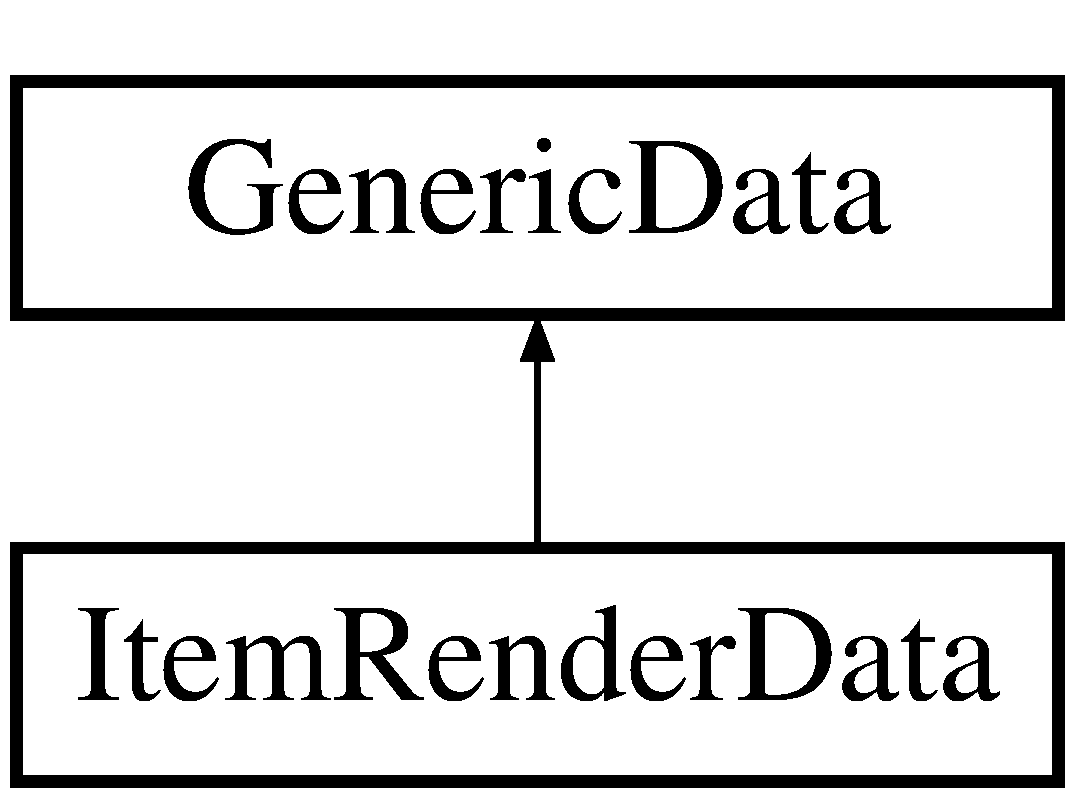
\includegraphics[height=2.000000cm]{class_item_render_data}
\end{center}
\end{figure}
\subsection*{Public Member Functions}
\begin{DoxyCompactItemize}
\item 
\hyperlink{class_item_render_data_a0723c1d09d574fbff96266c59ad7f480}{Item\-Render\-Data} (std\-::string filename)
\item 
\hyperlink{class_item_render_data_a195a4e545e323c4d32fc02a6eeec0a8c}{Item\-Render\-Data} ()
\item 
\hyperlink{class_item_render_data_a0242f6a6149a9e3945b8a2fd7faa2575}{$\sim$\-Item\-Render\-Data} ()
\item 
virtual void \hyperlink{class_item_render_data_a13f92fc9e5386ef04fb736fbacc17a7e}{write} (std\-::ostream \&out) const 
\item 
virtual void \hyperlink{class_item_render_data_afbda96d49108440c6ce4a9c0b541116f}{read} (std\-::istream \&in)
\end{DoxyCompactItemize}
\subsection*{Public Attributes}
\begin{DoxyCompactItemize}
\item 
double \hyperlink{class_item_render_data_ab75e41c0c3d9e0ab4a5eea05ff72be73}{m\-Painter\-Radius1}
\item 
double \hyperlink{class_item_render_data_aecdd63385a831142e8bb1e77168b4760}{m\-Painter\-Radius2}
\item 
double \hyperlink{class_item_render_data_a201e4edce1dc946735ea9b1b90f5990b}{m\-Painter\-Theta\-Dot}
\item 
\hyperlink{class_electric_material_data}{Electric\-Material\-Data} \hyperlink{class_item_render_data_ab57bb1aa34ce4b24269bada5366444fd}{m\-Painter\-Material}
\item 
double \hyperlink{class_item_render_data_ae553cbe13ede2dee4a95a15fb8c37725}{m\-End\-Radius1}
\item 
double \hyperlink{class_item_render_data_a879d26693545905b5f6289702b73b5e4}{m\-End\-Radius2}
\item 
double \hyperlink{class_item_render_data_add72dc0e3376793b72dae1b1fe36e965}{m\-End\-Theta\-Dot}
\item 
\hyperlink{class_electric_material_data}{Electric\-Material\-Data} \hyperlink{class_item_render_data_a95ad5539006fc0dacd26c02ab7209f57}{m\-End\-Material}
\end{DoxyCompactItemize}


\subsection{Constructor \& Destructor Documentation}
\hypertarget{class_item_render_data_a0723c1d09d574fbff96266c59ad7f480}{\index{Item\-Render\-Data@{Item\-Render\-Data}!Item\-Render\-Data@{Item\-Render\-Data}}
\index{Item\-Render\-Data@{Item\-Render\-Data}!ItemRenderData@{Item\-Render\-Data}}
\subsubsection[{Item\-Render\-Data}]{\setlength{\rightskip}{0pt plus 5cm}Item\-Render\-Data\-::\-Item\-Render\-Data (
\begin{DoxyParamCaption}
\item[{std\-::string}]{filename}
\end{DoxyParamCaption}
)}}\label{class_item_render_data_a0723c1d09d574fbff96266c59ad7f480}
\hypertarget{class_item_render_data_a195a4e545e323c4d32fc02a6eeec0a8c}{\index{Item\-Render\-Data@{Item\-Render\-Data}!Item\-Render\-Data@{Item\-Render\-Data}}
\index{Item\-Render\-Data@{Item\-Render\-Data}!ItemRenderData@{Item\-Render\-Data}}
\subsubsection[{Item\-Render\-Data}]{\setlength{\rightskip}{0pt plus 5cm}Item\-Render\-Data\-::\-Item\-Render\-Data (
\begin{DoxyParamCaption}
{}
\end{DoxyParamCaption}
)}}\label{class_item_render_data_a195a4e545e323c4d32fc02a6eeec0a8c}
\hypertarget{class_item_render_data_a0242f6a6149a9e3945b8a2fd7faa2575}{\index{Item\-Render\-Data@{Item\-Render\-Data}!$\sim$\-Item\-Render\-Data@{$\sim$\-Item\-Render\-Data}}
\index{$\sim$\-Item\-Render\-Data@{$\sim$\-Item\-Render\-Data}!ItemRenderData@{Item\-Render\-Data}}
\subsubsection[{$\sim$\-Item\-Render\-Data}]{\setlength{\rightskip}{0pt plus 5cm}Item\-Render\-Data\-::$\sim$\-Item\-Render\-Data (
\begin{DoxyParamCaption}
{}
\end{DoxyParamCaption}
)}}\label{class_item_render_data_a0242f6a6149a9e3945b8a2fd7faa2575}


\subsection{Member Function Documentation}
\hypertarget{class_item_render_data_afbda96d49108440c6ce4a9c0b541116f}{\index{Item\-Render\-Data@{Item\-Render\-Data}!read@{read}}
\index{read@{read}!ItemRenderData@{Item\-Render\-Data}}
\subsubsection[{read}]{\setlength{\rightskip}{0pt plus 5cm}void Item\-Render\-Data\-::read (
\begin{DoxyParamCaption}
\item[{std\-::istream \&}]{in}
\end{DoxyParamCaption}
)\hspace{0.3cm}{\ttfamily [virtual]}}}\label{class_item_render_data_afbda96d49108440c6ce4a9c0b541116f}


Implements \hyperlink{class_generic_data_a71e231ef04c9a91a3429123dab5bd1e7}{Generic\-Data}.

\hypertarget{class_item_render_data_a13f92fc9e5386ef04fb736fbacc17a7e}{\index{Item\-Render\-Data@{Item\-Render\-Data}!write@{write}}
\index{write@{write}!ItemRenderData@{Item\-Render\-Data}}
\subsubsection[{write}]{\setlength{\rightskip}{0pt plus 5cm}void Item\-Render\-Data\-::write (
\begin{DoxyParamCaption}
\item[{std\-::ostream \&}]{out}
\end{DoxyParamCaption}
) const\hspace{0.3cm}{\ttfamily [virtual]}}}\label{class_item_render_data_a13f92fc9e5386ef04fb736fbacc17a7e}


Implements \hyperlink{class_generic_data_a93ea61de5b09cf3fc95564ef3d841214}{Generic\-Data}.



\subsection{Member Data Documentation}
\hypertarget{class_item_render_data_a95ad5539006fc0dacd26c02ab7209f57}{\index{Item\-Render\-Data@{Item\-Render\-Data}!m\-End\-Material@{m\-End\-Material}}
\index{m\-End\-Material@{m\-End\-Material}!ItemRenderData@{Item\-Render\-Data}}
\subsubsection[{m\-End\-Material}]{\setlength{\rightskip}{0pt plus 5cm}{\bf Electric\-Material\-Data} Item\-Render\-Data\-::m\-End\-Material}}\label{class_item_render_data_a95ad5539006fc0dacd26c02ab7209f57}
\hypertarget{class_item_render_data_ae553cbe13ede2dee4a95a15fb8c37725}{\index{Item\-Render\-Data@{Item\-Render\-Data}!m\-End\-Radius1@{m\-End\-Radius1}}
\index{m\-End\-Radius1@{m\-End\-Radius1}!ItemRenderData@{Item\-Render\-Data}}
\subsubsection[{m\-End\-Radius1}]{\setlength{\rightskip}{0pt plus 5cm}double Item\-Render\-Data\-::m\-End\-Radius1}}\label{class_item_render_data_ae553cbe13ede2dee4a95a15fb8c37725}
\hypertarget{class_item_render_data_a879d26693545905b5f6289702b73b5e4}{\index{Item\-Render\-Data@{Item\-Render\-Data}!m\-End\-Radius2@{m\-End\-Radius2}}
\index{m\-End\-Radius2@{m\-End\-Radius2}!ItemRenderData@{Item\-Render\-Data}}
\subsubsection[{m\-End\-Radius2}]{\setlength{\rightskip}{0pt plus 5cm}double Item\-Render\-Data\-::m\-End\-Radius2}}\label{class_item_render_data_a879d26693545905b5f6289702b73b5e4}
\hypertarget{class_item_render_data_add72dc0e3376793b72dae1b1fe36e965}{\index{Item\-Render\-Data@{Item\-Render\-Data}!m\-End\-Theta\-Dot@{m\-End\-Theta\-Dot}}
\index{m\-End\-Theta\-Dot@{m\-End\-Theta\-Dot}!ItemRenderData@{Item\-Render\-Data}}
\subsubsection[{m\-End\-Theta\-Dot}]{\setlength{\rightskip}{0pt plus 5cm}double Item\-Render\-Data\-::m\-End\-Theta\-Dot}}\label{class_item_render_data_add72dc0e3376793b72dae1b1fe36e965}
\hypertarget{class_item_render_data_ab57bb1aa34ce4b24269bada5366444fd}{\index{Item\-Render\-Data@{Item\-Render\-Data}!m\-Painter\-Material@{m\-Painter\-Material}}
\index{m\-Painter\-Material@{m\-Painter\-Material}!ItemRenderData@{Item\-Render\-Data}}
\subsubsection[{m\-Painter\-Material}]{\setlength{\rightskip}{0pt plus 5cm}{\bf Electric\-Material\-Data} Item\-Render\-Data\-::m\-Painter\-Material}}\label{class_item_render_data_ab57bb1aa34ce4b24269bada5366444fd}
\hypertarget{class_item_render_data_ab75e41c0c3d9e0ab4a5eea05ff72be73}{\index{Item\-Render\-Data@{Item\-Render\-Data}!m\-Painter\-Radius1@{m\-Painter\-Radius1}}
\index{m\-Painter\-Radius1@{m\-Painter\-Radius1}!ItemRenderData@{Item\-Render\-Data}}
\subsubsection[{m\-Painter\-Radius1}]{\setlength{\rightskip}{0pt plus 5cm}double Item\-Render\-Data\-::m\-Painter\-Radius1}}\label{class_item_render_data_ab75e41c0c3d9e0ab4a5eea05ff72be73}
\hypertarget{class_item_render_data_aecdd63385a831142e8bb1e77168b4760}{\index{Item\-Render\-Data@{Item\-Render\-Data}!m\-Painter\-Radius2@{m\-Painter\-Radius2}}
\index{m\-Painter\-Radius2@{m\-Painter\-Radius2}!ItemRenderData@{Item\-Render\-Data}}
\subsubsection[{m\-Painter\-Radius2}]{\setlength{\rightskip}{0pt plus 5cm}double Item\-Render\-Data\-::m\-Painter\-Radius2}}\label{class_item_render_data_aecdd63385a831142e8bb1e77168b4760}
\hypertarget{class_item_render_data_a201e4edce1dc946735ea9b1b90f5990b}{\index{Item\-Render\-Data@{Item\-Render\-Data}!m\-Painter\-Theta\-Dot@{m\-Painter\-Theta\-Dot}}
\index{m\-Painter\-Theta\-Dot@{m\-Painter\-Theta\-Dot}!ItemRenderData@{Item\-Render\-Data}}
\subsubsection[{m\-Painter\-Theta\-Dot}]{\setlength{\rightskip}{0pt plus 5cm}double Item\-Render\-Data\-::m\-Painter\-Theta\-Dot}}\label{class_item_render_data_a201e4edce1dc946735ea9b1b90f5990b}


The documentation for this class was generated from the following files\-:\begin{DoxyCompactItemize}
\item 
C\-:/\-Users/\-Owner/\-My Programming/\-Personal Projects/\-Video\-Games/\-Optimist Racing/src/\hyperlink{_data_8hpp}{Data.\-hpp}\item 
C\-:/\-Users/\-Owner/\-My Programming/\-Personal Projects/\-Video\-Games/\-Optimist Racing/src/\hyperlink{_data_8cpp}{Data.\-cpp}\end{DoxyCompactItemize}

\hypertarget{class_lagrange_1_1_lagrangian_coordinates}{\section{Lagrange\-:\-:Lagrangian\-Coordinates Class Reference}
\label{class_lagrange_1_1_lagrangian_coordinates}\index{Lagrange\-::\-Lagrangian\-Coordinates@{Lagrange\-::\-Lagrangian\-Coordinates}}
}


{\ttfamily \#include $<$Lagrange.\-hpp$>$}

\subsection*{Public Member Functions}
\begin{DoxyCompactItemize}
\item 
\hyperlink{class_lagrange_1_1_lagrangian_coordinates_ab638b2f6e4e59bdd5e93bfa8c9eae9b4}{Lagrangian\-Coordinates} (int n)
\item 
\hyperlink{class_lagrange_1_1_lagrangian_coordinates_a70e1868a6825dbaddcebf5cf0c1b6b30}{$\sim$\-Lagrangian\-Coordinates} ()
\end{DoxyCompactItemize}


\subsection{Constructor \& Destructor Documentation}
\hypertarget{class_lagrange_1_1_lagrangian_coordinates_ab638b2f6e4e59bdd5e93bfa8c9eae9b4}{\index{Lagrange\-::\-Lagrangian\-Coordinates@{Lagrange\-::\-Lagrangian\-Coordinates}!Lagrangian\-Coordinates@{Lagrangian\-Coordinates}}
\index{Lagrangian\-Coordinates@{Lagrangian\-Coordinates}!Lagrange::LagrangianCoordinates@{Lagrange\-::\-Lagrangian\-Coordinates}}
\subsubsection[{Lagrangian\-Coordinates}]{\setlength{\rightskip}{0pt plus 5cm}Lagrange\-::\-Lagrangian\-Coordinates\-::\-Lagrangian\-Coordinates (
\begin{DoxyParamCaption}
\item[{int}]{n}
\end{DoxyParamCaption}
)}}\label{class_lagrange_1_1_lagrangian_coordinates_ab638b2f6e4e59bdd5e93bfa8c9eae9b4}
\hypertarget{class_lagrange_1_1_lagrangian_coordinates_a70e1868a6825dbaddcebf5cf0c1b6b30}{\index{Lagrange\-::\-Lagrangian\-Coordinates@{Lagrange\-::\-Lagrangian\-Coordinates}!$\sim$\-Lagrangian\-Coordinates@{$\sim$\-Lagrangian\-Coordinates}}
\index{$\sim$\-Lagrangian\-Coordinates@{$\sim$\-Lagrangian\-Coordinates}!Lagrange::LagrangianCoordinates@{Lagrange\-::\-Lagrangian\-Coordinates}}
\subsubsection[{$\sim$\-Lagrangian\-Coordinates}]{\setlength{\rightskip}{0pt plus 5cm}Lagrange\-::\-Lagrangian\-Coordinates\-::$\sim$\-Lagrangian\-Coordinates (
\begin{DoxyParamCaption}
{}
\end{DoxyParamCaption}
)}}\label{class_lagrange_1_1_lagrangian_coordinates_a70e1868a6825dbaddcebf5cf0c1b6b30}


The documentation for this class was generated from the following file\-:\begin{DoxyCompactItemize}
\item 
C\-:/\-Users/\-Owner/\-My Programming/\-Personal Projects/\-Video\-Games/\-Optimist Racing/src/\hyperlink{_lagrange_8hpp}{Lagrange.\-hpp}\end{DoxyCompactItemize}

\hypertarget{class_lagrange_1_1_lagrangian_object}{\section{Lagrange\-:\-:Lagrangian\-Object Class Reference}
\label{class_lagrange_1_1_lagrangian_object}\index{Lagrange\-::\-Lagrangian\-Object@{Lagrange\-::\-Lagrangian\-Object}}
}


{\ttfamily \#include $<$Lagrange.\-hpp$>$}

\subsection*{Public Member Functions}
\begin{DoxyCompactItemize}
\item 
\hyperlink{class_lagrange_1_1_lagrangian_object_a4d3e40326aa8904ef0f6df757d0ffa36}{Lagrangian\-Object} ()
\item 
\hyperlink{class_lagrange_1_1_lagrangian_object_a7b8af43209f370fa73e9ef80315decd2}{$\sim$\-Lagrangian\-Object} ()
\item 
double \hyperlink{class_lagrange_1_1_lagrangian_object_a492e12e6f8d293c133469b9dad0cf12c}{get\-X} ()
\item 
double \hyperlink{class_lagrange_1_1_lagrangian_object_a7909222d7950aadb3ad245e93f561284}{get\-Y} ()
\item 
double \hyperlink{class_lagrange_1_1_lagrangian_object_aec714f96a67ced912894f185b8d6b467}{get\-Z} ()
\item 
double \hyperlink{class_lagrange_1_1_lagrangian_object_aa5d4da3f10ddc6e0030ab9c498da5af4}{get\-Alpha} ()
\item 
double \hyperlink{class_lagrange_1_1_lagrangian_object_a25d5a657520a100f3d8a1cf01343ad08}{get\-Beta} ()
\item 
double \hyperlink{class_lagrange_1_1_lagrangian_object_a8a439494a8efe728068f39e39f21a5b6}{get\-Gamma} ()
\end{DoxyCompactItemize}


\subsection{Constructor \& Destructor Documentation}
\hypertarget{class_lagrange_1_1_lagrangian_object_a4d3e40326aa8904ef0f6df757d0ffa36}{\index{Lagrange\-::\-Lagrangian\-Object@{Lagrange\-::\-Lagrangian\-Object}!Lagrangian\-Object@{Lagrangian\-Object}}
\index{Lagrangian\-Object@{Lagrangian\-Object}!Lagrange::LagrangianObject@{Lagrange\-::\-Lagrangian\-Object}}
\subsubsection[{Lagrangian\-Object}]{\setlength{\rightskip}{0pt plus 5cm}Lagrange\-::\-Lagrangian\-Object\-::\-Lagrangian\-Object (
\begin{DoxyParamCaption}
{}
\end{DoxyParamCaption}
)}}\label{class_lagrange_1_1_lagrangian_object_a4d3e40326aa8904ef0f6df757d0ffa36}
\hypertarget{class_lagrange_1_1_lagrangian_object_a7b8af43209f370fa73e9ef80315decd2}{\index{Lagrange\-::\-Lagrangian\-Object@{Lagrange\-::\-Lagrangian\-Object}!$\sim$\-Lagrangian\-Object@{$\sim$\-Lagrangian\-Object}}
\index{$\sim$\-Lagrangian\-Object@{$\sim$\-Lagrangian\-Object}!Lagrange::LagrangianObject@{Lagrange\-::\-Lagrangian\-Object}}
\subsubsection[{$\sim$\-Lagrangian\-Object}]{\setlength{\rightskip}{0pt plus 5cm}Lagrange\-::\-Lagrangian\-Object\-::$\sim$\-Lagrangian\-Object (
\begin{DoxyParamCaption}
{}
\end{DoxyParamCaption}
)}}\label{class_lagrange_1_1_lagrangian_object_a7b8af43209f370fa73e9ef80315decd2}


\subsection{Member Function Documentation}
\hypertarget{class_lagrange_1_1_lagrangian_object_aa5d4da3f10ddc6e0030ab9c498da5af4}{\index{Lagrange\-::\-Lagrangian\-Object@{Lagrange\-::\-Lagrangian\-Object}!get\-Alpha@{get\-Alpha}}
\index{get\-Alpha@{get\-Alpha}!Lagrange::LagrangianObject@{Lagrange\-::\-Lagrangian\-Object}}
\subsubsection[{get\-Alpha}]{\setlength{\rightskip}{0pt plus 5cm}double Lagrange\-::\-Lagrangian\-Object\-::get\-Alpha (
\begin{DoxyParamCaption}
{}
\end{DoxyParamCaption}
)}}\label{class_lagrange_1_1_lagrangian_object_aa5d4da3f10ddc6e0030ab9c498da5af4}
\hypertarget{class_lagrange_1_1_lagrangian_object_a25d5a657520a100f3d8a1cf01343ad08}{\index{Lagrange\-::\-Lagrangian\-Object@{Lagrange\-::\-Lagrangian\-Object}!get\-Beta@{get\-Beta}}
\index{get\-Beta@{get\-Beta}!Lagrange::LagrangianObject@{Lagrange\-::\-Lagrangian\-Object}}
\subsubsection[{get\-Beta}]{\setlength{\rightskip}{0pt plus 5cm}double Lagrange\-::\-Lagrangian\-Object\-::get\-Beta (
\begin{DoxyParamCaption}
{}
\end{DoxyParamCaption}
)}}\label{class_lagrange_1_1_lagrangian_object_a25d5a657520a100f3d8a1cf01343ad08}
\hypertarget{class_lagrange_1_1_lagrangian_object_a8a439494a8efe728068f39e39f21a5b6}{\index{Lagrange\-::\-Lagrangian\-Object@{Lagrange\-::\-Lagrangian\-Object}!get\-Gamma@{get\-Gamma}}
\index{get\-Gamma@{get\-Gamma}!Lagrange::LagrangianObject@{Lagrange\-::\-Lagrangian\-Object}}
\subsubsection[{get\-Gamma}]{\setlength{\rightskip}{0pt plus 5cm}double Lagrange\-::\-Lagrangian\-Object\-::get\-Gamma (
\begin{DoxyParamCaption}
{}
\end{DoxyParamCaption}
)}}\label{class_lagrange_1_1_lagrangian_object_a8a439494a8efe728068f39e39f21a5b6}
\hypertarget{class_lagrange_1_1_lagrangian_object_a492e12e6f8d293c133469b9dad0cf12c}{\index{Lagrange\-::\-Lagrangian\-Object@{Lagrange\-::\-Lagrangian\-Object}!get\-X@{get\-X}}
\index{get\-X@{get\-X}!Lagrange::LagrangianObject@{Lagrange\-::\-Lagrangian\-Object}}
\subsubsection[{get\-X}]{\setlength{\rightskip}{0pt plus 5cm}double Lagrange\-::\-Lagrangian\-Object\-::get\-X (
\begin{DoxyParamCaption}
{}
\end{DoxyParamCaption}
)}}\label{class_lagrange_1_1_lagrangian_object_a492e12e6f8d293c133469b9dad0cf12c}
\hypertarget{class_lagrange_1_1_lagrangian_object_a7909222d7950aadb3ad245e93f561284}{\index{Lagrange\-::\-Lagrangian\-Object@{Lagrange\-::\-Lagrangian\-Object}!get\-Y@{get\-Y}}
\index{get\-Y@{get\-Y}!Lagrange::LagrangianObject@{Lagrange\-::\-Lagrangian\-Object}}
\subsubsection[{get\-Y}]{\setlength{\rightskip}{0pt plus 5cm}double Lagrange\-::\-Lagrangian\-Object\-::get\-Y (
\begin{DoxyParamCaption}
{}
\end{DoxyParamCaption}
)}}\label{class_lagrange_1_1_lagrangian_object_a7909222d7950aadb3ad245e93f561284}
\hypertarget{class_lagrange_1_1_lagrangian_object_aec714f96a67ced912894f185b8d6b467}{\index{Lagrange\-::\-Lagrangian\-Object@{Lagrange\-::\-Lagrangian\-Object}!get\-Z@{get\-Z}}
\index{get\-Z@{get\-Z}!Lagrange::LagrangianObject@{Lagrange\-::\-Lagrangian\-Object}}
\subsubsection[{get\-Z}]{\setlength{\rightskip}{0pt plus 5cm}double Lagrange\-::\-Lagrangian\-Object\-::get\-Z (
\begin{DoxyParamCaption}
{}
\end{DoxyParamCaption}
)}}\label{class_lagrange_1_1_lagrangian_object_aec714f96a67ced912894f185b8d6b467}


The documentation for this class was generated from the following file\-:\begin{DoxyCompactItemize}
\item 
C\-:/\-Users/\-Owner/\-My Programming/\-Personal Projects/\-Video\-Games/\-Optimist Racing/src/\hyperlink{_lagrange_8hpp}{Lagrange.\-hpp}\end{DoxyCompactItemize}

\hypertarget{class_lagrange_1_1_lagrangian_racer}{\section{Lagrange\-:\-:Lagrangian\-Racer Class Reference}
\label{class_lagrange_1_1_lagrangian_racer}\index{Lagrange\-::\-Lagrangian\-Racer@{Lagrange\-::\-Lagrangian\-Racer}}
}


{\ttfamily \#include $<$Lagrange.\-hpp$>$}

\subsection*{Public Member Functions}
\begin{DoxyCompactItemize}
\item 
\hyperlink{class_lagrange_1_1_lagrangian_racer_ae92c8f69443f3674b7e769693de16635}{Lagrangian\-Racer} (const \hyperlink{class_bezier_patch_grid}{Bezier\-Patch\-Grid} $\ast$bezier\-Patch\-Grid, double gravity, double length, double mass\-Bottom, double mass\-Top, double I\-Bottom, double I\-Top\-X, double I\-Top\-Y, double I\-Top\-Z, double xdotmax, double ydotmax, double zdotmax, double thetadotmax, double phidotmax, double x, double y, double theta, double phi, double xdot, double ydot, double thetadot, double phidot)
\item 
\hyperlink{class_lagrange_1_1_lagrangian_racer_afb798998c0432ca5cf2654e97e57c7eb}{$\sim$\-Lagrangian\-Racer} ()
\item 
\hyperlink{class_lagrange_1_1_lagrangian_racer}{Lagrangian\-Racer} $\ast$ \hyperlink{class_lagrange_1_1_lagrangian_racer_a92f67f8a32e94105f10f20c9910e9bab}{create} (const \hyperlink{class_bezier_patch_grid}{Bezier\-Patch\-Grid} $\ast$bezier\-Patch\-Grid, double gravity, double size, double x, double y, double theta, double phi, double xdot, double ydot, double thetadot, double phidot)
\item 
const \hyperlink{class_bezier_patch_grid}{Bezier\-Patch\-Grid} $\ast$ \hyperlink{class_lagrange_1_1_lagrangian_racer_a4145112e6b98ed5fe2e074c16c33267b}{get\-Bezier\-Patch\-Grid} () const 
\item 
double \hyperlink{class_lagrange_1_1_lagrangian_racer_ab65063aa5eaa49d85b9b10fe9f4b5208}{get\-Gravity} () const 
\item 
double \hyperlink{class_lagrange_1_1_lagrangian_racer_a321343be8922996016777cd6ecb566a9}{get\-Length} () const 
\item 
double \hyperlink{class_lagrange_1_1_lagrangian_racer_a3ba71f2ce0d789f86921f293cbf22294}{get\-Mass\-Bottom} () const 
\item 
double \hyperlink{class_lagrange_1_1_lagrangian_racer_a09dd99ca786308a18fb1d245ecbbbfd0}{get\-Mass\-Top} () const 
\item 
double \hyperlink{class_lagrange_1_1_lagrangian_racer_a04ad64e40b927f28d96d7bb458c68e4b}{get\-I\-Bottom} () const 
\item 
double \hyperlink{class_lagrange_1_1_lagrangian_racer_a30894c02d07bc862496cc9554b1a16e2}{get\-I\-Top\-X} () const 
\item 
double \hyperlink{class_lagrange_1_1_lagrangian_racer_aa8d89ff48c8a7bf3def041f9dd539901}{get\-I\-Top\-Y} () const 
\item 
double \hyperlink{class_lagrange_1_1_lagrangian_racer_abd471e7837c867c0f6f16b47a4cd3d14}{get\-I\-Top\-Z} () const 
\item 
double \hyperlink{class_lagrange_1_1_lagrangian_racer_a79220d9bc1c5b6f32d5cafe69dcf050b}{get\-X} () const 
\item 
double \hyperlink{class_lagrange_1_1_lagrangian_racer_a563536fe789d0283b9fc82f3a5b6a9ff}{get\-Y} () const 
\item 
double \hyperlink{class_lagrange_1_1_lagrangian_racer_a8cf4e66e33ac4cffdca6e7f0f1b14e61}{get\-Z} () const 
\item 
double \hyperlink{class_lagrange_1_1_lagrangian_racer_a4ad3d8b75a18350919469dc7165ea4dd}{get\-Theta} () const 
\item 
double \hyperlink{class_lagrange_1_1_lagrangian_racer_ae4a0f8ebfcc28911cde0233567d19cc1}{get\-Phi} () const 
\item 
double \hyperlink{class_lagrange_1_1_lagrangian_racer_a1bbbf1c37947a5414f047555bf375ec1}{get\-X\-Dot} () const 
\item 
double \hyperlink{class_lagrange_1_1_lagrangian_racer_a0f9b25e09ddef578e644a920d7064d9f}{get\-Y\-Dot} () const 
\item 
double \hyperlink{class_lagrange_1_1_lagrangian_racer_a490a9e8912b1299c92b6e2daec17c9b0}{get\-Z\-Dot} () const 
\item 
double \hyperlink{class_lagrange_1_1_lagrangian_racer_ae84b2dde39fbe737bdb9d3401e9d23f9}{get\-Theta\-Dot} () const 
\item 
double \hyperlink{class_lagrange_1_1_lagrangian_racer_a58963b1269a427232451a17ec9485c1c}{get\-Phi\-Dot} () const 
\item 
\hyperlink{class_vector3_d}{Vector3\-D} \hyperlink{class_lagrange_1_1_lagrangian_racer_aafd2da89d986b558ce77bc3f572c34dc}{get\-Bottom\-Position} () const 
\item 
\hyperlink{class_vector3_d}{Vector3\-D} \hyperlink{class_lagrange_1_1_lagrangian_racer_ace39268853f7088cc984ea72b78d63c7}{get\-Top\-Position} () const 
\item 
void \hyperlink{class_lagrange_1_1_lagrangian_racer_ad54dda570366844b036db2fea60120c4}{clear\-Forces} ()
\item 
void \hyperlink{class_lagrange_1_1_lagrangian_racer_a972b438060163d865de9e3d52714a995}{set\-Force\-Bottom\-World} (const \hyperlink{class_vector3_d}{Vector3\-D} \&force)
\item 
void \hyperlink{class_lagrange_1_1_lagrangian_racer_a353eb3b9f1cefe5b09bfebf75cf09587}{set\-Force\-Top\-World} (const \hyperlink{class_vector3_d}{Vector3\-D} \&force)
\item 
void \hyperlink{class_lagrange_1_1_lagrangian_racer_abe7a4e8d86ac16426c393abe85f58b6f}{set\-Force\-Bottom\-Model} (const \hyperlink{class_vector3_d}{Vector3\-D} \&force)
\item 
void \hyperlink{class_lagrange_1_1_lagrangian_racer_a9590ef3a0d4ef15af3fffbefc3ff1ecf}{set\-Force\-Top\-Model} (const \hyperlink{class_vector3_d}{Vector3\-D} \&force)
\item 
void \hyperlink{class_lagrange_1_1_lagrangian_racer_ade76dfca80d5084c25efb884d271080e}{set\-Torque\-Bottom\-Model\-Z} (double torque)
\item 
void \hyperlink{class_lagrange_1_1_lagrangian_racer_a5e1e87c22da38dffd72eb2f1c2a3a748}{set\-Torque\-Bottom\-Model} (const \hyperlink{class_vector3_d}{Vector3\-D} \&torque)
\item 
void \hyperlink{class_lagrange_1_1_lagrangian_racer_ae7dd23c80c9708efc7eb57d8ba88bfab}{set\-Torque\-Top\-Model} (const \hyperlink{class_vector3_d}{Vector3\-D} \&torque)
\item 
void \hyperlink{class_lagrange_1_1_lagrangian_racer_a29249707fa1a0be9c433a74e043d4294}{set\-Torque\-Top\-World} (const \hyperlink{class_vector3_d}{Vector3\-D} \&torque)
\item 
void \hyperlink{class_lagrange_1_1_lagrangian_racer_aa9366243d714865b601d81d10f4e6dce}{add\-Force\-Bottom\-World} (const \hyperlink{class_vector3_d}{Vector3\-D} \&force)
\item 
void \hyperlink{class_lagrange_1_1_lagrangian_racer_a853814ef5e85ed91b5d21285f45f3483}{add\-Force\-Top\-World} (const \hyperlink{class_vector3_d}{Vector3\-D} \&force)
\item 
void \hyperlink{class_lagrange_1_1_lagrangian_racer_a7aaf93c05924f525995d837a16d23a28}{add\-Force\-Bottom\-Model} (const \hyperlink{class_vector3_d}{Vector3\-D} \&force)
\item 
void \hyperlink{class_lagrange_1_1_lagrangian_racer_a19901db0943f63fae28667b751bb1bf4}{add\-Force\-Top\-Model} (const \hyperlink{class_vector3_d}{Vector3\-D} \&force)
\item 
void \hyperlink{class_lagrange_1_1_lagrangian_racer_a28b28f9259ce4cbaf6ebd5b056c61c8f}{add\-Torque\-Bottom\-Model\-Z} (double torque)
\item 
void \hyperlink{class_lagrange_1_1_lagrangian_racer_a3dc8d7072a7370907e1b82efd50a6b58}{add\-Torque\-Bottom\-Model} (const \hyperlink{class_vector3_d}{Vector3\-D} \&torque)
\item 
void \hyperlink{class_lagrange_1_1_lagrangian_racer_a1ac741a8d3a369c3a62c487a7ae79d7a}{add\-Torque\-Top\-Model} (const \hyperlink{class_vector3_d}{Vector3\-D} \&torque)
\item 
void \hyperlink{class_lagrange_1_1_lagrangian_racer_a8fff6f5f11dc051c712c924f43251dfe}{add\-Torque\-Top\-World} (const \hyperlink{class_vector3_d}{Vector3\-D} \&torque)
\item 
void \hyperlink{class_lagrange_1_1_lagrangian_racer_addb45d891a16d0b839be8d10f2fcd557}{step\-Racing} (double seconds)
\item 
void \hyperlink{class_lagrange_1_1_lagrangian_racer_a53288dff55d60e9bce9564e5e30b6652}{step\-Flying} (double seconds)
\item 
void \hyperlink{class_lagrange_1_1_lagrangian_racer_a1d34f95637932a0402e90aef7b4d7d64}{land} ()
\end{DoxyCompactItemize}


\subsection{Constructor \& Destructor Documentation}
\hypertarget{class_lagrange_1_1_lagrangian_racer_ae92c8f69443f3674b7e769693de16635}{\index{Lagrange\-::\-Lagrangian\-Racer@{Lagrange\-::\-Lagrangian\-Racer}!Lagrangian\-Racer@{Lagrangian\-Racer}}
\index{Lagrangian\-Racer@{Lagrangian\-Racer}!Lagrange::LagrangianRacer@{Lagrange\-::\-Lagrangian\-Racer}}
\subsubsection[{Lagrangian\-Racer}]{\setlength{\rightskip}{0pt plus 5cm}Lagrange\-::\-Lagrangian\-Racer\-::\-Lagrangian\-Racer (
\begin{DoxyParamCaption}
\item[{const {\bf Bezier\-Patch\-Grid} $\ast$}]{bezier\-Patch\-Grid, }
\item[{double}]{gravity, }
\item[{double}]{length, }
\item[{double}]{mass\-Bottom, }
\item[{double}]{mass\-Top, }
\item[{double}]{I\-Bottom, }
\item[{double}]{I\-Top\-X, }
\item[{double}]{I\-Top\-Y, }
\item[{double}]{I\-Top\-Z, }
\item[{double}]{xdotmax, }
\item[{double}]{ydotmax, }
\item[{double}]{zdotmax, }
\item[{double}]{thetadotmax, }
\item[{double}]{phidotmax, }
\item[{double}]{x, }
\item[{double}]{y, }
\item[{double}]{theta, }
\item[{double}]{phi, }
\item[{double}]{xdot, }
\item[{double}]{ydot, }
\item[{double}]{thetadot, }
\item[{double}]{phidot}
\end{DoxyParamCaption}
)}}\label{class_lagrange_1_1_lagrangian_racer_ae92c8f69443f3674b7e769693de16635}
\hypertarget{class_lagrange_1_1_lagrangian_racer_afb798998c0432ca5cf2654e97e57c7eb}{\index{Lagrange\-::\-Lagrangian\-Racer@{Lagrange\-::\-Lagrangian\-Racer}!$\sim$\-Lagrangian\-Racer@{$\sim$\-Lagrangian\-Racer}}
\index{$\sim$\-Lagrangian\-Racer@{$\sim$\-Lagrangian\-Racer}!Lagrange::LagrangianRacer@{Lagrange\-::\-Lagrangian\-Racer}}
\subsubsection[{$\sim$\-Lagrangian\-Racer}]{\setlength{\rightskip}{0pt plus 5cm}Lagrange\-::\-Lagrangian\-Racer\-::$\sim$\-Lagrangian\-Racer (
\begin{DoxyParamCaption}
{}
\end{DoxyParamCaption}
)}}\label{class_lagrange_1_1_lagrangian_racer_afb798998c0432ca5cf2654e97e57c7eb}


\subsection{Member Function Documentation}
\hypertarget{class_lagrange_1_1_lagrangian_racer_a7aaf93c05924f525995d837a16d23a28}{\index{Lagrange\-::\-Lagrangian\-Racer@{Lagrange\-::\-Lagrangian\-Racer}!add\-Force\-Bottom\-Model@{add\-Force\-Bottom\-Model}}
\index{add\-Force\-Bottom\-Model@{add\-Force\-Bottom\-Model}!Lagrange::LagrangianRacer@{Lagrange\-::\-Lagrangian\-Racer}}
\subsubsection[{add\-Force\-Bottom\-Model}]{\setlength{\rightskip}{0pt plus 5cm}void Lagrange\-::\-Lagrangian\-Racer\-::add\-Force\-Bottom\-Model (
\begin{DoxyParamCaption}
\item[{const {\bf Vector3\-D} \&}]{force}
\end{DoxyParamCaption}
)}}\label{class_lagrange_1_1_lagrangian_racer_a7aaf93c05924f525995d837a16d23a28}
\hypertarget{class_lagrange_1_1_lagrangian_racer_aa9366243d714865b601d81d10f4e6dce}{\index{Lagrange\-::\-Lagrangian\-Racer@{Lagrange\-::\-Lagrangian\-Racer}!add\-Force\-Bottom\-World@{add\-Force\-Bottom\-World}}
\index{add\-Force\-Bottom\-World@{add\-Force\-Bottom\-World}!Lagrange::LagrangianRacer@{Lagrange\-::\-Lagrangian\-Racer}}
\subsubsection[{add\-Force\-Bottom\-World}]{\setlength{\rightskip}{0pt plus 5cm}void Lagrange\-::\-Lagrangian\-Racer\-::add\-Force\-Bottom\-World (
\begin{DoxyParamCaption}
\item[{const {\bf Vector3\-D} \&}]{force}
\end{DoxyParamCaption}
)}}\label{class_lagrange_1_1_lagrangian_racer_aa9366243d714865b601d81d10f4e6dce}
\hypertarget{class_lagrange_1_1_lagrangian_racer_a19901db0943f63fae28667b751bb1bf4}{\index{Lagrange\-::\-Lagrangian\-Racer@{Lagrange\-::\-Lagrangian\-Racer}!add\-Force\-Top\-Model@{add\-Force\-Top\-Model}}
\index{add\-Force\-Top\-Model@{add\-Force\-Top\-Model}!Lagrange::LagrangianRacer@{Lagrange\-::\-Lagrangian\-Racer}}
\subsubsection[{add\-Force\-Top\-Model}]{\setlength{\rightskip}{0pt plus 5cm}void Lagrange\-::\-Lagrangian\-Racer\-::add\-Force\-Top\-Model (
\begin{DoxyParamCaption}
\item[{const {\bf Vector3\-D} \&}]{force}
\end{DoxyParamCaption}
)}}\label{class_lagrange_1_1_lagrangian_racer_a19901db0943f63fae28667b751bb1bf4}
\hypertarget{class_lagrange_1_1_lagrangian_racer_a853814ef5e85ed91b5d21285f45f3483}{\index{Lagrange\-::\-Lagrangian\-Racer@{Lagrange\-::\-Lagrangian\-Racer}!add\-Force\-Top\-World@{add\-Force\-Top\-World}}
\index{add\-Force\-Top\-World@{add\-Force\-Top\-World}!Lagrange::LagrangianRacer@{Lagrange\-::\-Lagrangian\-Racer}}
\subsubsection[{add\-Force\-Top\-World}]{\setlength{\rightskip}{0pt plus 5cm}void Lagrange\-::\-Lagrangian\-Racer\-::add\-Force\-Top\-World (
\begin{DoxyParamCaption}
\item[{const {\bf Vector3\-D} \&}]{force}
\end{DoxyParamCaption}
)}}\label{class_lagrange_1_1_lagrangian_racer_a853814ef5e85ed91b5d21285f45f3483}
\hypertarget{class_lagrange_1_1_lagrangian_racer_a3dc8d7072a7370907e1b82efd50a6b58}{\index{Lagrange\-::\-Lagrangian\-Racer@{Lagrange\-::\-Lagrangian\-Racer}!add\-Torque\-Bottom\-Model@{add\-Torque\-Bottom\-Model}}
\index{add\-Torque\-Bottom\-Model@{add\-Torque\-Bottom\-Model}!Lagrange::LagrangianRacer@{Lagrange\-::\-Lagrangian\-Racer}}
\subsubsection[{add\-Torque\-Bottom\-Model}]{\setlength{\rightskip}{0pt plus 5cm}void Lagrange\-::\-Lagrangian\-Racer\-::add\-Torque\-Bottom\-Model (
\begin{DoxyParamCaption}
\item[{const {\bf Vector3\-D} \&}]{torque}
\end{DoxyParamCaption}
)}}\label{class_lagrange_1_1_lagrangian_racer_a3dc8d7072a7370907e1b82efd50a6b58}
\hypertarget{class_lagrange_1_1_lagrangian_racer_a28b28f9259ce4cbaf6ebd5b056c61c8f}{\index{Lagrange\-::\-Lagrangian\-Racer@{Lagrange\-::\-Lagrangian\-Racer}!add\-Torque\-Bottom\-Model\-Z@{add\-Torque\-Bottom\-Model\-Z}}
\index{add\-Torque\-Bottom\-Model\-Z@{add\-Torque\-Bottom\-Model\-Z}!Lagrange::LagrangianRacer@{Lagrange\-::\-Lagrangian\-Racer}}
\subsubsection[{add\-Torque\-Bottom\-Model\-Z}]{\setlength{\rightskip}{0pt plus 5cm}void Lagrange\-::\-Lagrangian\-Racer\-::add\-Torque\-Bottom\-Model\-Z (
\begin{DoxyParamCaption}
\item[{double}]{torque}
\end{DoxyParamCaption}
)}}\label{class_lagrange_1_1_lagrangian_racer_a28b28f9259ce4cbaf6ebd5b056c61c8f}
\hypertarget{class_lagrange_1_1_lagrangian_racer_a1ac741a8d3a369c3a62c487a7ae79d7a}{\index{Lagrange\-::\-Lagrangian\-Racer@{Lagrange\-::\-Lagrangian\-Racer}!add\-Torque\-Top\-Model@{add\-Torque\-Top\-Model}}
\index{add\-Torque\-Top\-Model@{add\-Torque\-Top\-Model}!Lagrange::LagrangianRacer@{Lagrange\-::\-Lagrangian\-Racer}}
\subsubsection[{add\-Torque\-Top\-Model}]{\setlength{\rightskip}{0pt plus 5cm}void Lagrange\-::\-Lagrangian\-Racer\-::add\-Torque\-Top\-Model (
\begin{DoxyParamCaption}
\item[{const {\bf Vector3\-D} \&}]{torque}
\end{DoxyParamCaption}
)}}\label{class_lagrange_1_1_lagrangian_racer_a1ac741a8d3a369c3a62c487a7ae79d7a}
\hypertarget{class_lagrange_1_1_lagrangian_racer_a8fff6f5f11dc051c712c924f43251dfe}{\index{Lagrange\-::\-Lagrangian\-Racer@{Lagrange\-::\-Lagrangian\-Racer}!add\-Torque\-Top\-World@{add\-Torque\-Top\-World}}
\index{add\-Torque\-Top\-World@{add\-Torque\-Top\-World}!Lagrange::LagrangianRacer@{Lagrange\-::\-Lagrangian\-Racer}}
\subsubsection[{add\-Torque\-Top\-World}]{\setlength{\rightskip}{0pt plus 5cm}void Lagrange\-::\-Lagrangian\-Racer\-::add\-Torque\-Top\-World (
\begin{DoxyParamCaption}
\item[{const {\bf Vector3\-D} \&}]{torque}
\end{DoxyParamCaption}
)}}\label{class_lagrange_1_1_lagrangian_racer_a8fff6f5f11dc051c712c924f43251dfe}
\hypertarget{class_lagrange_1_1_lagrangian_racer_ad54dda570366844b036db2fea60120c4}{\index{Lagrange\-::\-Lagrangian\-Racer@{Lagrange\-::\-Lagrangian\-Racer}!clear\-Forces@{clear\-Forces}}
\index{clear\-Forces@{clear\-Forces}!Lagrange::LagrangianRacer@{Lagrange\-::\-Lagrangian\-Racer}}
\subsubsection[{clear\-Forces}]{\setlength{\rightskip}{0pt plus 5cm}void Lagrange\-::\-Lagrangian\-Racer\-::clear\-Forces (
\begin{DoxyParamCaption}
{}
\end{DoxyParamCaption}
)}}\label{class_lagrange_1_1_lagrangian_racer_ad54dda570366844b036db2fea60120c4}
\hypertarget{class_lagrange_1_1_lagrangian_racer_a92f67f8a32e94105f10f20c9910e9bab}{\index{Lagrange\-::\-Lagrangian\-Racer@{Lagrange\-::\-Lagrangian\-Racer}!create@{create}}
\index{create@{create}!Lagrange::LagrangianRacer@{Lagrange\-::\-Lagrangian\-Racer}}
\subsubsection[{create}]{\setlength{\rightskip}{0pt plus 5cm}{\bf Lagrangian\-Racer} $\ast$ Lagrange\-::\-Lagrangian\-Racer\-::create (
\begin{DoxyParamCaption}
\item[{const {\bf Bezier\-Patch\-Grid} $\ast$}]{bezier\-Patch\-Grid, }
\item[{double}]{gravity, }
\item[{double}]{size, }
\item[{double}]{x, }
\item[{double}]{y, }
\item[{double}]{theta, }
\item[{double}]{phi, }
\item[{double}]{xdot, }
\item[{double}]{ydot, }
\item[{double}]{thetadot, }
\item[{double}]{phidot}
\end{DoxyParamCaption}
)}}\label{class_lagrange_1_1_lagrangian_racer_a92f67f8a32e94105f10f20c9910e9bab}
\hypertarget{class_lagrange_1_1_lagrangian_racer_a4145112e6b98ed5fe2e074c16c33267b}{\index{Lagrange\-::\-Lagrangian\-Racer@{Lagrange\-::\-Lagrangian\-Racer}!get\-Bezier\-Patch\-Grid@{get\-Bezier\-Patch\-Grid}}
\index{get\-Bezier\-Patch\-Grid@{get\-Bezier\-Patch\-Grid}!Lagrange::LagrangianRacer@{Lagrange\-::\-Lagrangian\-Racer}}
\subsubsection[{get\-Bezier\-Patch\-Grid}]{\setlength{\rightskip}{0pt plus 5cm}const {\bf Bezier\-Patch\-Grid} $\ast$ Lagrange\-::\-Lagrangian\-Racer\-::get\-Bezier\-Patch\-Grid (
\begin{DoxyParamCaption}
{}
\end{DoxyParamCaption}
) const}}\label{class_lagrange_1_1_lagrangian_racer_a4145112e6b98ed5fe2e074c16c33267b}
\hypertarget{class_lagrange_1_1_lagrangian_racer_aafd2da89d986b558ce77bc3f572c34dc}{\index{Lagrange\-::\-Lagrangian\-Racer@{Lagrange\-::\-Lagrangian\-Racer}!get\-Bottom\-Position@{get\-Bottom\-Position}}
\index{get\-Bottom\-Position@{get\-Bottom\-Position}!Lagrange::LagrangianRacer@{Lagrange\-::\-Lagrangian\-Racer}}
\subsubsection[{get\-Bottom\-Position}]{\setlength{\rightskip}{0pt plus 5cm}{\bf Vector3\-D} Lagrange\-::\-Lagrangian\-Racer\-::get\-Bottom\-Position (
\begin{DoxyParamCaption}
{}
\end{DoxyParamCaption}
) const}}\label{class_lagrange_1_1_lagrangian_racer_aafd2da89d986b558ce77bc3f572c34dc}
\hypertarget{class_lagrange_1_1_lagrangian_racer_ab65063aa5eaa49d85b9b10fe9f4b5208}{\index{Lagrange\-::\-Lagrangian\-Racer@{Lagrange\-::\-Lagrangian\-Racer}!get\-Gravity@{get\-Gravity}}
\index{get\-Gravity@{get\-Gravity}!Lagrange::LagrangianRacer@{Lagrange\-::\-Lagrangian\-Racer}}
\subsubsection[{get\-Gravity}]{\setlength{\rightskip}{0pt plus 5cm}double Lagrange\-::\-Lagrangian\-Racer\-::get\-Gravity (
\begin{DoxyParamCaption}
{}
\end{DoxyParamCaption}
) const}}\label{class_lagrange_1_1_lagrangian_racer_ab65063aa5eaa49d85b9b10fe9f4b5208}
\hypertarget{class_lagrange_1_1_lagrangian_racer_a04ad64e40b927f28d96d7bb458c68e4b}{\index{Lagrange\-::\-Lagrangian\-Racer@{Lagrange\-::\-Lagrangian\-Racer}!get\-I\-Bottom@{get\-I\-Bottom}}
\index{get\-I\-Bottom@{get\-I\-Bottom}!Lagrange::LagrangianRacer@{Lagrange\-::\-Lagrangian\-Racer}}
\subsubsection[{get\-I\-Bottom}]{\setlength{\rightskip}{0pt plus 5cm}double Lagrange\-::\-Lagrangian\-Racer\-::get\-I\-Bottom (
\begin{DoxyParamCaption}
{}
\end{DoxyParamCaption}
) const}}\label{class_lagrange_1_1_lagrangian_racer_a04ad64e40b927f28d96d7bb458c68e4b}
\hypertarget{class_lagrange_1_1_lagrangian_racer_a30894c02d07bc862496cc9554b1a16e2}{\index{Lagrange\-::\-Lagrangian\-Racer@{Lagrange\-::\-Lagrangian\-Racer}!get\-I\-Top\-X@{get\-I\-Top\-X}}
\index{get\-I\-Top\-X@{get\-I\-Top\-X}!Lagrange::LagrangianRacer@{Lagrange\-::\-Lagrangian\-Racer}}
\subsubsection[{get\-I\-Top\-X}]{\setlength{\rightskip}{0pt plus 5cm}double Lagrange\-::\-Lagrangian\-Racer\-::get\-I\-Top\-X (
\begin{DoxyParamCaption}
{}
\end{DoxyParamCaption}
) const}}\label{class_lagrange_1_1_lagrangian_racer_a30894c02d07bc862496cc9554b1a16e2}
\hypertarget{class_lagrange_1_1_lagrangian_racer_aa8d89ff48c8a7bf3def041f9dd539901}{\index{Lagrange\-::\-Lagrangian\-Racer@{Lagrange\-::\-Lagrangian\-Racer}!get\-I\-Top\-Y@{get\-I\-Top\-Y}}
\index{get\-I\-Top\-Y@{get\-I\-Top\-Y}!Lagrange::LagrangianRacer@{Lagrange\-::\-Lagrangian\-Racer}}
\subsubsection[{get\-I\-Top\-Y}]{\setlength{\rightskip}{0pt plus 5cm}double Lagrange\-::\-Lagrangian\-Racer\-::get\-I\-Top\-Y (
\begin{DoxyParamCaption}
{}
\end{DoxyParamCaption}
) const}}\label{class_lagrange_1_1_lagrangian_racer_aa8d89ff48c8a7bf3def041f9dd539901}
\hypertarget{class_lagrange_1_1_lagrangian_racer_abd471e7837c867c0f6f16b47a4cd3d14}{\index{Lagrange\-::\-Lagrangian\-Racer@{Lagrange\-::\-Lagrangian\-Racer}!get\-I\-Top\-Z@{get\-I\-Top\-Z}}
\index{get\-I\-Top\-Z@{get\-I\-Top\-Z}!Lagrange::LagrangianRacer@{Lagrange\-::\-Lagrangian\-Racer}}
\subsubsection[{get\-I\-Top\-Z}]{\setlength{\rightskip}{0pt plus 5cm}double Lagrange\-::\-Lagrangian\-Racer\-::get\-I\-Top\-Z (
\begin{DoxyParamCaption}
{}
\end{DoxyParamCaption}
) const}}\label{class_lagrange_1_1_lagrangian_racer_abd471e7837c867c0f6f16b47a4cd3d14}
\hypertarget{class_lagrange_1_1_lagrangian_racer_a321343be8922996016777cd6ecb566a9}{\index{Lagrange\-::\-Lagrangian\-Racer@{Lagrange\-::\-Lagrangian\-Racer}!get\-Length@{get\-Length}}
\index{get\-Length@{get\-Length}!Lagrange::LagrangianRacer@{Lagrange\-::\-Lagrangian\-Racer}}
\subsubsection[{get\-Length}]{\setlength{\rightskip}{0pt plus 5cm}double Lagrange\-::\-Lagrangian\-Racer\-::get\-Length (
\begin{DoxyParamCaption}
{}
\end{DoxyParamCaption}
) const}}\label{class_lagrange_1_1_lagrangian_racer_a321343be8922996016777cd6ecb566a9}
\hypertarget{class_lagrange_1_1_lagrangian_racer_a3ba71f2ce0d789f86921f293cbf22294}{\index{Lagrange\-::\-Lagrangian\-Racer@{Lagrange\-::\-Lagrangian\-Racer}!get\-Mass\-Bottom@{get\-Mass\-Bottom}}
\index{get\-Mass\-Bottom@{get\-Mass\-Bottom}!Lagrange::LagrangianRacer@{Lagrange\-::\-Lagrangian\-Racer}}
\subsubsection[{get\-Mass\-Bottom}]{\setlength{\rightskip}{0pt plus 5cm}double Lagrange\-::\-Lagrangian\-Racer\-::get\-Mass\-Bottom (
\begin{DoxyParamCaption}
{}
\end{DoxyParamCaption}
) const}}\label{class_lagrange_1_1_lagrangian_racer_a3ba71f2ce0d789f86921f293cbf22294}
\hypertarget{class_lagrange_1_1_lagrangian_racer_a09dd99ca786308a18fb1d245ecbbbfd0}{\index{Lagrange\-::\-Lagrangian\-Racer@{Lagrange\-::\-Lagrangian\-Racer}!get\-Mass\-Top@{get\-Mass\-Top}}
\index{get\-Mass\-Top@{get\-Mass\-Top}!Lagrange::LagrangianRacer@{Lagrange\-::\-Lagrangian\-Racer}}
\subsubsection[{get\-Mass\-Top}]{\setlength{\rightskip}{0pt plus 5cm}double Lagrange\-::\-Lagrangian\-Racer\-::get\-Mass\-Top (
\begin{DoxyParamCaption}
{}
\end{DoxyParamCaption}
) const}}\label{class_lagrange_1_1_lagrangian_racer_a09dd99ca786308a18fb1d245ecbbbfd0}
\hypertarget{class_lagrange_1_1_lagrangian_racer_ae4a0f8ebfcc28911cde0233567d19cc1}{\index{Lagrange\-::\-Lagrangian\-Racer@{Lagrange\-::\-Lagrangian\-Racer}!get\-Phi@{get\-Phi}}
\index{get\-Phi@{get\-Phi}!Lagrange::LagrangianRacer@{Lagrange\-::\-Lagrangian\-Racer}}
\subsubsection[{get\-Phi}]{\setlength{\rightskip}{0pt plus 5cm}double Lagrange\-::\-Lagrangian\-Racer\-::get\-Phi (
\begin{DoxyParamCaption}
{}
\end{DoxyParamCaption}
) const}}\label{class_lagrange_1_1_lagrangian_racer_ae4a0f8ebfcc28911cde0233567d19cc1}
\hypertarget{class_lagrange_1_1_lagrangian_racer_a58963b1269a427232451a17ec9485c1c}{\index{Lagrange\-::\-Lagrangian\-Racer@{Lagrange\-::\-Lagrangian\-Racer}!get\-Phi\-Dot@{get\-Phi\-Dot}}
\index{get\-Phi\-Dot@{get\-Phi\-Dot}!Lagrange::LagrangianRacer@{Lagrange\-::\-Lagrangian\-Racer}}
\subsubsection[{get\-Phi\-Dot}]{\setlength{\rightskip}{0pt plus 5cm}double Lagrange\-::\-Lagrangian\-Racer\-::get\-Phi\-Dot (
\begin{DoxyParamCaption}
{}
\end{DoxyParamCaption}
) const}}\label{class_lagrange_1_1_lagrangian_racer_a58963b1269a427232451a17ec9485c1c}
\hypertarget{class_lagrange_1_1_lagrangian_racer_a4ad3d8b75a18350919469dc7165ea4dd}{\index{Lagrange\-::\-Lagrangian\-Racer@{Lagrange\-::\-Lagrangian\-Racer}!get\-Theta@{get\-Theta}}
\index{get\-Theta@{get\-Theta}!Lagrange::LagrangianRacer@{Lagrange\-::\-Lagrangian\-Racer}}
\subsubsection[{get\-Theta}]{\setlength{\rightskip}{0pt plus 5cm}double Lagrange\-::\-Lagrangian\-Racer\-::get\-Theta (
\begin{DoxyParamCaption}
{}
\end{DoxyParamCaption}
) const}}\label{class_lagrange_1_1_lagrangian_racer_a4ad3d8b75a18350919469dc7165ea4dd}
\hypertarget{class_lagrange_1_1_lagrangian_racer_ae84b2dde39fbe737bdb9d3401e9d23f9}{\index{Lagrange\-::\-Lagrangian\-Racer@{Lagrange\-::\-Lagrangian\-Racer}!get\-Theta\-Dot@{get\-Theta\-Dot}}
\index{get\-Theta\-Dot@{get\-Theta\-Dot}!Lagrange::LagrangianRacer@{Lagrange\-::\-Lagrangian\-Racer}}
\subsubsection[{get\-Theta\-Dot}]{\setlength{\rightskip}{0pt plus 5cm}double Lagrange\-::\-Lagrangian\-Racer\-::get\-Theta\-Dot (
\begin{DoxyParamCaption}
{}
\end{DoxyParamCaption}
) const}}\label{class_lagrange_1_1_lagrangian_racer_ae84b2dde39fbe737bdb9d3401e9d23f9}
\hypertarget{class_lagrange_1_1_lagrangian_racer_ace39268853f7088cc984ea72b78d63c7}{\index{Lagrange\-::\-Lagrangian\-Racer@{Lagrange\-::\-Lagrangian\-Racer}!get\-Top\-Position@{get\-Top\-Position}}
\index{get\-Top\-Position@{get\-Top\-Position}!Lagrange::LagrangianRacer@{Lagrange\-::\-Lagrangian\-Racer}}
\subsubsection[{get\-Top\-Position}]{\setlength{\rightskip}{0pt plus 5cm}{\bf Vector3\-D} Lagrange\-::\-Lagrangian\-Racer\-::get\-Top\-Position (
\begin{DoxyParamCaption}
{}
\end{DoxyParamCaption}
) const}}\label{class_lagrange_1_1_lagrangian_racer_ace39268853f7088cc984ea72b78d63c7}
\hypertarget{class_lagrange_1_1_lagrangian_racer_a79220d9bc1c5b6f32d5cafe69dcf050b}{\index{Lagrange\-::\-Lagrangian\-Racer@{Lagrange\-::\-Lagrangian\-Racer}!get\-X@{get\-X}}
\index{get\-X@{get\-X}!Lagrange::LagrangianRacer@{Lagrange\-::\-Lagrangian\-Racer}}
\subsubsection[{get\-X}]{\setlength{\rightskip}{0pt plus 5cm}double Lagrange\-::\-Lagrangian\-Racer\-::get\-X (
\begin{DoxyParamCaption}
{}
\end{DoxyParamCaption}
) const}}\label{class_lagrange_1_1_lagrangian_racer_a79220d9bc1c5b6f32d5cafe69dcf050b}
\hypertarget{class_lagrange_1_1_lagrangian_racer_a1bbbf1c37947a5414f047555bf375ec1}{\index{Lagrange\-::\-Lagrangian\-Racer@{Lagrange\-::\-Lagrangian\-Racer}!get\-X\-Dot@{get\-X\-Dot}}
\index{get\-X\-Dot@{get\-X\-Dot}!Lagrange::LagrangianRacer@{Lagrange\-::\-Lagrangian\-Racer}}
\subsubsection[{get\-X\-Dot}]{\setlength{\rightskip}{0pt plus 5cm}double Lagrange\-::\-Lagrangian\-Racer\-::get\-X\-Dot (
\begin{DoxyParamCaption}
{}
\end{DoxyParamCaption}
) const}}\label{class_lagrange_1_1_lagrangian_racer_a1bbbf1c37947a5414f047555bf375ec1}
\hypertarget{class_lagrange_1_1_lagrangian_racer_a563536fe789d0283b9fc82f3a5b6a9ff}{\index{Lagrange\-::\-Lagrangian\-Racer@{Lagrange\-::\-Lagrangian\-Racer}!get\-Y@{get\-Y}}
\index{get\-Y@{get\-Y}!Lagrange::LagrangianRacer@{Lagrange\-::\-Lagrangian\-Racer}}
\subsubsection[{get\-Y}]{\setlength{\rightskip}{0pt plus 5cm}double Lagrange\-::\-Lagrangian\-Racer\-::get\-Y (
\begin{DoxyParamCaption}
{}
\end{DoxyParamCaption}
) const}}\label{class_lagrange_1_1_lagrangian_racer_a563536fe789d0283b9fc82f3a5b6a9ff}
\hypertarget{class_lagrange_1_1_lagrangian_racer_a0f9b25e09ddef578e644a920d7064d9f}{\index{Lagrange\-::\-Lagrangian\-Racer@{Lagrange\-::\-Lagrangian\-Racer}!get\-Y\-Dot@{get\-Y\-Dot}}
\index{get\-Y\-Dot@{get\-Y\-Dot}!Lagrange::LagrangianRacer@{Lagrange\-::\-Lagrangian\-Racer}}
\subsubsection[{get\-Y\-Dot}]{\setlength{\rightskip}{0pt plus 5cm}double Lagrange\-::\-Lagrangian\-Racer\-::get\-Y\-Dot (
\begin{DoxyParamCaption}
{}
\end{DoxyParamCaption}
) const}}\label{class_lagrange_1_1_lagrangian_racer_a0f9b25e09ddef578e644a920d7064d9f}
\hypertarget{class_lagrange_1_1_lagrangian_racer_a8cf4e66e33ac4cffdca6e7f0f1b14e61}{\index{Lagrange\-::\-Lagrangian\-Racer@{Lagrange\-::\-Lagrangian\-Racer}!get\-Z@{get\-Z}}
\index{get\-Z@{get\-Z}!Lagrange::LagrangianRacer@{Lagrange\-::\-Lagrangian\-Racer}}
\subsubsection[{get\-Z}]{\setlength{\rightskip}{0pt plus 5cm}double Lagrange\-::\-Lagrangian\-Racer\-::get\-Z (
\begin{DoxyParamCaption}
{}
\end{DoxyParamCaption}
) const}}\label{class_lagrange_1_1_lagrangian_racer_a8cf4e66e33ac4cffdca6e7f0f1b14e61}
\hypertarget{class_lagrange_1_1_lagrangian_racer_a490a9e8912b1299c92b6e2daec17c9b0}{\index{Lagrange\-::\-Lagrangian\-Racer@{Lagrange\-::\-Lagrangian\-Racer}!get\-Z\-Dot@{get\-Z\-Dot}}
\index{get\-Z\-Dot@{get\-Z\-Dot}!Lagrange::LagrangianRacer@{Lagrange\-::\-Lagrangian\-Racer}}
\subsubsection[{get\-Z\-Dot}]{\setlength{\rightskip}{0pt plus 5cm}double Lagrange\-::\-Lagrangian\-Racer\-::get\-Z\-Dot (
\begin{DoxyParamCaption}
{}
\end{DoxyParamCaption}
) const}}\label{class_lagrange_1_1_lagrangian_racer_a490a9e8912b1299c92b6e2daec17c9b0}
\hypertarget{class_lagrange_1_1_lagrangian_racer_a1d34f95637932a0402e90aef7b4d7d64}{\index{Lagrange\-::\-Lagrangian\-Racer@{Lagrange\-::\-Lagrangian\-Racer}!land@{land}}
\index{land@{land}!Lagrange::LagrangianRacer@{Lagrange\-::\-Lagrangian\-Racer}}
\subsubsection[{land}]{\setlength{\rightskip}{0pt plus 5cm}void Lagrange\-::\-Lagrangian\-Racer\-::land (
\begin{DoxyParamCaption}
{}
\end{DoxyParamCaption}
)}}\label{class_lagrange_1_1_lagrangian_racer_a1d34f95637932a0402e90aef7b4d7d64}
\hypertarget{class_lagrange_1_1_lagrangian_racer_abe7a4e8d86ac16426c393abe85f58b6f}{\index{Lagrange\-::\-Lagrangian\-Racer@{Lagrange\-::\-Lagrangian\-Racer}!set\-Force\-Bottom\-Model@{set\-Force\-Bottom\-Model}}
\index{set\-Force\-Bottom\-Model@{set\-Force\-Bottom\-Model}!Lagrange::LagrangianRacer@{Lagrange\-::\-Lagrangian\-Racer}}
\subsubsection[{set\-Force\-Bottom\-Model}]{\setlength{\rightskip}{0pt plus 5cm}void Lagrange\-::\-Lagrangian\-Racer\-::set\-Force\-Bottom\-Model (
\begin{DoxyParamCaption}
\item[{const {\bf Vector3\-D} \&}]{force}
\end{DoxyParamCaption}
)}}\label{class_lagrange_1_1_lagrangian_racer_abe7a4e8d86ac16426c393abe85f58b6f}
\hypertarget{class_lagrange_1_1_lagrangian_racer_a972b438060163d865de9e3d52714a995}{\index{Lagrange\-::\-Lagrangian\-Racer@{Lagrange\-::\-Lagrangian\-Racer}!set\-Force\-Bottom\-World@{set\-Force\-Bottom\-World}}
\index{set\-Force\-Bottom\-World@{set\-Force\-Bottom\-World}!Lagrange::LagrangianRacer@{Lagrange\-::\-Lagrangian\-Racer}}
\subsubsection[{set\-Force\-Bottom\-World}]{\setlength{\rightskip}{0pt plus 5cm}void Lagrange\-::\-Lagrangian\-Racer\-::set\-Force\-Bottom\-World (
\begin{DoxyParamCaption}
\item[{const {\bf Vector3\-D} \&}]{force}
\end{DoxyParamCaption}
)}}\label{class_lagrange_1_1_lagrangian_racer_a972b438060163d865de9e3d52714a995}
\hypertarget{class_lagrange_1_1_lagrangian_racer_a9590ef3a0d4ef15af3fffbefc3ff1ecf}{\index{Lagrange\-::\-Lagrangian\-Racer@{Lagrange\-::\-Lagrangian\-Racer}!set\-Force\-Top\-Model@{set\-Force\-Top\-Model}}
\index{set\-Force\-Top\-Model@{set\-Force\-Top\-Model}!Lagrange::LagrangianRacer@{Lagrange\-::\-Lagrangian\-Racer}}
\subsubsection[{set\-Force\-Top\-Model}]{\setlength{\rightskip}{0pt plus 5cm}void Lagrange\-::\-Lagrangian\-Racer\-::set\-Force\-Top\-Model (
\begin{DoxyParamCaption}
\item[{const {\bf Vector3\-D} \&}]{force}
\end{DoxyParamCaption}
)}}\label{class_lagrange_1_1_lagrangian_racer_a9590ef3a0d4ef15af3fffbefc3ff1ecf}
\hypertarget{class_lagrange_1_1_lagrangian_racer_a353eb3b9f1cefe5b09bfebf75cf09587}{\index{Lagrange\-::\-Lagrangian\-Racer@{Lagrange\-::\-Lagrangian\-Racer}!set\-Force\-Top\-World@{set\-Force\-Top\-World}}
\index{set\-Force\-Top\-World@{set\-Force\-Top\-World}!Lagrange::LagrangianRacer@{Lagrange\-::\-Lagrangian\-Racer}}
\subsubsection[{set\-Force\-Top\-World}]{\setlength{\rightskip}{0pt plus 5cm}void Lagrange\-::\-Lagrangian\-Racer\-::set\-Force\-Top\-World (
\begin{DoxyParamCaption}
\item[{const {\bf Vector3\-D} \&}]{force}
\end{DoxyParamCaption}
)}}\label{class_lagrange_1_1_lagrangian_racer_a353eb3b9f1cefe5b09bfebf75cf09587}
\hypertarget{class_lagrange_1_1_lagrangian_racer_a5e1e87c22da38dffd72eb2f1c2a3a748}{\index{Lagrange\-::\-Lagrangian\-Racer@{Lagrange\-::\-Lagrangian\-Racer}!set\-Torque\-Bottom\-Model@{set\-Torque\-Bottom\-Model}}
\index{set\-Torque\-Bottom\-Model@{set\-Torque\-Bottom\-Model}!Lagrange::LagrangianRacer@{Lagrange\-::\-Lagrangian\-Racer}}
\subsubsection[{set\-Torque\-Bottom\-Model}]{\setlength{\rightskip}{0pt plus 5cm}void Lagrange\-::\-Lagrangian\-Racer\-::set\-Torque\-Bottom\-Model (
\begin{DoxyParamCaption}
\item[{const {\bf Vector3\-D} \&}]{torque}
\end{DoxyParamCaption}
)}}\label{class_lagrange_1_1_lagrangian_racer_a5e1e87c22da38dffd72eb2f1c2a3a748}
\hypertarget{class_lagrange_1_1_lagrangian_racer_ade76dfca80d5084c25efb884d271080e}{\index{Lagrange\-::\-Lagrangian\-Racer@{Lagrange\-::\-Lagrangian\-Racer}!set\-Torque\-Bottom\-Model\-Z@{set\-Torque\-Bottom\-Model\-Z}}
\index{set\-Torque\-Bottom\-Model\-Z@{set\-Torque\-Bottom\-Model\-Z}!Lagrange::LagrangianRacer@{Lagrange\-::\-Lagrangian\-Racer}}
\subsubsection[{set\-Torque\-Bottom\-Model\-Z}]{\setlength{\rightskip}{0pt plus 5cm}void Lagrange\-::\-Lagrangian\-Racer\-::set\-Torque\-Bottom\-Model\-Z (
\begin{DoxyParamCaption}
\item[{double}]{torque}
\end{DoxyParamCaption}
)}}\label{class_lagrange_1_1_lagrangian_racer_ade76dfca80d5084c25efb884d271080e}
\hypertarget{class_lagrange_1_1_lagrangian_racer_ae7dd23c80c9708efc7eb57d8ba88bfab}{\index{Lagrange\-::\-Lagrangian\-Racer@{Lagrange\-::\-Lagrangian\-Racer}!set\-Torque\-Top\-Model@{set\-Torque\-Top\-Model}}
\index{set\-Torque\-Top\-Model@{set\-Torque\-Top\-Model}!Lagrange::LagrangianRacer@{Lagrange\-::\-Lagrangian\-Racer}}
\subsubsection[{set\-Torque\-Top\-Model}]{\setlength{\rightskip}{0pt plus 5cm}void Lagrange\-::\-Lagrangian\-Racer\-::set\-Torque\-Top\-Model (
\begin{DoxyParamCaption}
\item[{const {\bf Vector3\-D} \&}]{torque}
\end{DoxyParamCaption}
)}}\label{class_lagrange_1_1_lagrangian_racer_ae7dd23c80c9708efc7eb57d8ba88bfab}
\hypertarget{class_lagrange_1_1_lagrangian_racer_a29249707fa1a0be9c433a74e043d4294}{\index{Lagrange\-::\-Lagrangian\-Racer@{Lagrange\-::\-Lagrangian\-Racer}!set\-Torque\-Top\-World@{set\-Torque\-Top\-World}}
\index{set\-Torque\-Top\-World@{set\-Torque\-Top\-World}!Lagrange::LagrangianRacer@{Lagrange\-::\-Lagrangian\-Racer}}
\subsubsection[{set\-Torque\-Top\-World}]{\setlength{\rightskip}{0pt plus 5cm}void Lagrange\-::\-Lagrangian\-Racer\-::set\-Torque\-Top\-World (
\begin{DoxyParamCaption}
\item[{const {\bf Vector3\-D} \&}]{torque}
\end{DoxyParamCaption}
)}}\label{class_lagrange_1_1_lagrangian_racer_a29249707fa1a0be9c433a74e043d4294}
\hypertarget{class_lagrange_1_1_lagrangian_racer_a53288dff55d60e9bce9564e5e30b6652}{\index{Lagrange\-::\-Lagrangian\-Racer@{Lagrange\-::\-Lagrangian\-Racer}!step\-Flying@{step\-Flying}}
\index{step\-Flying@{step\-Flying}!Lagrange::LagrangianRacer@{Lagrange\-::\-Lagrangian\-Racer}}
\subsubsection[{step\-Flying}]{\setlength{\rightskip}{0pt plus 5cm}void Lagrange\-::\-Lagrangian\-Racer\-::step\-Flying (
\begin{DoxyParamCaption}
\item[{double}]{seconds}
\end{DoxyParamCaption}
)}}\label{class_lagrange_1_1_lagrangian_racer_a53288dff55d60e9bce9564e5e30b6652}
\hypertarget{class_lagrange_1_1_lagrangian_racer_addb45d891a16d0b839be8d10f2fcd557}{\index{Lagrange\-::\-Lagrangian\-Racer@{Lagrange\-::\-Lagrangian\-Racer}!step\-Racing@{step\-Racing}}
\index{step\-Racing@{step\-Racing}!Lagrange::LagrangianRacer@{Lagrange\-::\-Lagrangian\-Racer}}
\subsubsection[{step\-Racing}]{\setlength{\rightskip}{0pt plus 5cm}void Lagrange\-::\-Lagrangian\-Racer\-::step\-Racing (
\begin{DoxyParamCaption}
\item[{double}]{seconds}
\end{DoxyParamCaption}
)}}\label{class_lagrange_1_1_lagrangian_racer_addb45d891a16d0b839be8d10f2fcd557}


The documentation for this class was generated from the following files\-:\begin{DoxyCompactItemize}
\item 
C\-:/\-Users/\-Owner/\-My Programming/\-Personal Projects/\-Video\-Games/\-Optimist Racing/src/\hyperlink{_lagrange_8hpp}{Lagrange.\-hpp}\item 
C\-:/\-Users/\-Owner/\-My Programming/\-Personal Projects/\-Video\-Games/\-Optimist Racing/src/\hyperlink{_lagrange_8cpp}{Lagrange.\-cpp}\end{DoxyCompactItemize}

\hypertarget{class_lagrangian_racer_data}{\section{Lagrangian\-Racer\-Data Class Reference}
\label{class_lagrangian_racer_data}\index{Lagrangian\-Racer\-Data@{Lagrangian\-Racer\-Data}}
}


{\ttfamily \#include $<$Data.\-hpp$>$}

Inheritance diagram for Lagrangian\-Racer\-Data\-:\begin{figure}[H]
\begin{center}
\leavevmode
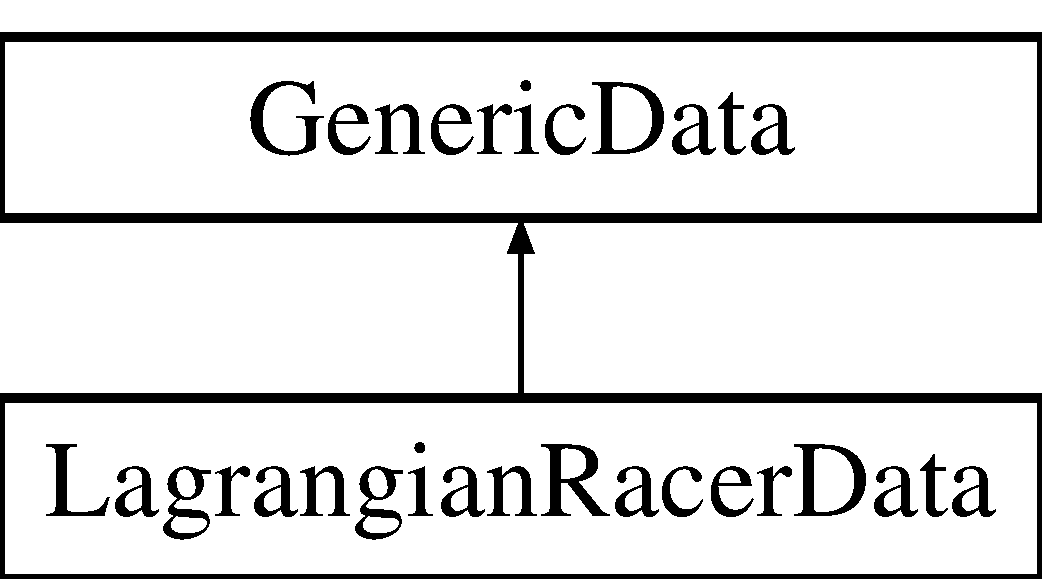
\includegraphics[height=2.000000cm]{class_lagrangian_racer_data}
\end{center}
\end{figure}
\subsection*{Public Member Functions}
\begin{DoxyCompactItemize}
\item 
\hyperlink{class_lagrangian_racer_data_a22776165f2f5e749a93238e4997f512e}{Lagrangian\-Racer\-Data} (std\-::string filename)
\item 
\hyperlink{class_lagrangian_racer_data_a4a07a05fba44af02d49fa689325dd809}{Lagrangian\-Racer\-Data} ()
\item 
\hyperlink{class_lagrangian_racer_data_aa643dd8a389074b4ef523a17f8c47423}{$\sim$\-Lagrangian\-Racer\-Data} ()
\item 
virtual void \hyperlink{class_lagrangian_racer_data_adbea50ddbb24883866bb828985fa6164}{write} (std\-::ostream \&out) const 
\item 
virtual void \hyperlink{class_lagrangian_racer_data_a5985c44e28872d0064596a3104f2feff}{read} (std\-::istream \&in)
\end{DoxyCompactItemize}
\subsection*{Public Attributes}
\begin{DoxyCompactItemize}
\item 
double \hyperlink{class_lagrangian_racer_data_a2c340e07fe3519f15e872a228f96bf24}{m\-Gravity}
\item 
double \hyperlink{class_lagrangian_racer_data_a2b78bd4a43be558d55b3415d4c10a32c}{m\-Length}
\item 
double \hyperlink{class_lagrangian_racer_data_a1ceba8b9818f1e838029136579a2ae0b}{m\-Head\-Radius}
\item 
double \hyperlink{class_lagrangian_racer_data_ad374a97e1a9c895af9a03e5149085fff}{m\-Body\-Radius}
\item 
double \hyperlink{class_lagrangian_racer_data_a41117d72e1cec8183499670f106df028}{m\-Bottom\-Radius}
\item 
double \hyperlink{class_lagrangian_racer_data_afd955e790601a655e78bca4427214e4d}{m\-Head\-Mass}
\item 
double \hyperlink{class_lagrangian_racer_data_a5c5db20c2be3befd438610dd3e2e0cab}{m\-Body\-Mass}
\item 
double \hyperlink{class_lagrangian_racer_data_a4753daf5933b5682f24238a4ce8ff826}{m\-Bottom\-Mass}
\item 
double \hyperlink{class_lagrangian_racer_data_a1ae8b9a4774c97eada607bea3588e12c}{m\-X\-Y\-Z\-Dot\-Max}
\item 
double \hyperlink{class_lagrangian_racer_data_a675af79a245f4b87be42c231fc2a0cb4}{m\-Theta\-Dot\-Max}
\item 
double \hyperlink{class_lagrangian_racer_data_ae29fef4cc2252ff093469d86344fd500}{m\-Phi\-Dot\-Max}
\item 
double \hyperlink{class_lagrangian_racer_data_a41ce1797ecc7d474dfa1facf87215c68}{m\-Start\-X}
\item 
double \hyperlink{class_lagrangian_racer_data_a54d64aa25b1892898ade2ba0db033289}{m\-Start\-Y}
\item 
double \hyperlink{class_lagrangian_racer_data_a7c08ebeb85dd7ba4860a843d9423217d}{m\-Start\-Theta}
\item 
double \hyperlink{class_lagrangian_racer_data_a8bebb8cb938477d7daeefe3c3c09d333}{m\-Start\-Phi}
\item 
double \hyperlink{class_lagrangian_racer_data_acb10387e8f9696008a48c9d3d917ffd3}{m\-Start\-X\-Dot}
\item 
double \hyperlink{class_lagrangian_racer_data_a6a7c78ce9de7ffcbb33be68528e5517d}{m\-Start\-Y\-Dot}
\item 
double \hyperlink{class_lagrangian_racer_data_af212142cc23b6798c64977ca0b67fce6}{m\-Start\-Theta\-Dot}
\item 
double \hyperlink{class_lagrangian_racer_data_a5b070020860e2f56f80855f5d9156b8a}{m\-Start\-Phi\-Dot}
\item 
\hyperlink{_electric_colour_8hpp_a1979e84576b59c4d100d8a8cc41de734}{E\-\_\-\-E\-L\-E\-C\-T\-R\-I\-C\-C\-O\-L\-O\-U\-R} \hyperlink{class_lagrangian_racer_data_a3923456f0f9cd5ef72d7ac03f0a328ef}{m\-Colour}
\item 
double \hyperlink{class_lagrangian_racer_data_aee2f252fb96173df52f960d1e5d6d472}{m\-Force\-Multiplier\-Right}
\item 
double \hyperlink{class_lagrangian_racer_data_a3850b3722529380cede99e7c55630f00}{m\-Force\-Multiplier\-Up}
\item 
double \hyperlink{class_lagrangian_racer_data_ad8276c8d2a904ed4eeda7590cc12cf25}{m\-Torque\-Multiplier}
\end{DoxyCompactItemize}


\subsection{Constructor \& Destructor Documentation}
\hypertarget{class_lagrangian_racer_data_a22776165f2f5e749a93238e4997f512e}{\index{Lagrangian\-Racer\-Data@{Lagrangian\-Racer\-Data}!Lagrangian\-Racer\-Data@{Lagrangian\-Racer\-Data}}
\index{Lagrangian\-Racer\-Data@{Lagrangian\-Racer\-Data}!LagrangianRacerData@{Lagrangian\-Racer\-Data}}
\subsubsection[{Lagrangian\-Racer\-Data}]{\setlength{\rightskip}{0pt plus 5cm}Lagrangian\-Racer\-Data\-::\-Lagrangian\-Racer\-Data (
\begin{DoxyParamCaption}
\item[{std\-::string}]{filename}
\end{DoxyParamCaption}
)}}\label{class_lagrangian_racer_data_a22776165f2f5e749a93238e4997f512e}
\hypertarget{class_lagrangian_racer_data_a4a07a05fba44af02d49fa689325dd809}{\index{Lagrangian\-Racer\-Data@{Lagrangian\-Racer\-Data}!Lagrangian\-Racer\-Data@{Lagrangian\-Racer\-Data}}
\index{Lagrangian\-Racer\-Data@{Lagrangian\-Racer\-Data}!LagrangianRacerData@{Lagrangian\-Racer\-Data}}
\subsubsection[{Lagrangian\-Racer\-Data}]{\setlength{\rightskip}{0pt plus 5cm}Lagrangian\-Racer\-Data\-::\-Lagrangian\-Racer\-Data (
\begin{DoxyParamCaption}
{}
\end{DoxyParamCaption}
)}}\label{class_lagrangian_racer_data_a4a07a05fba44af02d49fa689325dd809}
\hypertarget{class_lagrangian_racer_data_aa643dd8a389074b4ef523a17f8c47423}{\index{Lagrangian\-Racer\-Data@{Lagrangian\-Racer\-Data}!$\sim$\-Lagrangian\-Racer\-Data@{$\sim$\-Lagrangian\-Racer\-Data}}
\index{$\sim$\-Lagrangian\-Racer\-Data@{$\sim$\-Lagrangian\-Racer\-Data}!LagrangianRacerData@{Lagrangian\-Racer\-Data}}
\subsubsection[{$\sim$\-Lagrangian\-Racer\-Data}]{\setlength{\rightskip}{0pt plus 5cm}Lagrangian\-Racer\-Data\-::$\sim$\-Lagrangian\-Racer\-Data (
\begin{DoxyParamCaption}
{}
\end{DoxyParamCaption}
)}}\label{class_lagrangian_racer_data_aa643dd8a389074b4ef523a17f8c47423}


\subsection{Member Function Documentation}
\hypertarget{class_lagrangian_racer_data_a5985c44e28872d0064596a3104f2feff}{\index{Lagrangian\-Racer\-Data@{Lagrangian\-Racer\-Data}!read@{read}}
\index{read@{read}!LagrangianRacerData@{Lagrangian\-Racer\-Data}}
\subsubsection[{read}]{\setlength{\rightskip}{0pt plus 5cm}void Lagrangian\-Racer\-Data\-::read (
\begin{DoxyParamCaption}
\item[{std\-::istream \&}]{in}
\end{DoxyParamCaption}
)\hspace{0.3cm}{\ttfamily [virtual]}}}\label{class_lagrangian_racer_data_a5985c44e28872d0064596a3104f2feff}


Implements \hyperlink{class_generic_data_a71e231ef04c9a91a3429123dab5bd1e7}{Generic\-Data}.

\hypertarget{class_lagrangian_racer_data_adbea50ddbb24883866bb828985fa6164}{\index{Lagrangian\-Racer\-Data@{Lagrangian\-Racer\-Data}!write@{write}}
\index{write@{write}!LagrangianRacerData@{Lagrangian\-Racer\-Data}}
\subsubsection[{write}]{\setlength{\rightskip}{0pt plus 5cm}void Lagrangian\-Racer\-Data\-::write (
\begin{DoxyParamCaption}
\item[{std\-::ostream \&}]{out}
\end{DoxyParamCaption}
) const\hspace{0.3cm}{\ttfamily [virtual]}}}\label{class_lagrangian_racer_data_adbea50ddbb24883866bb828985fa6164}


Implements \hyperlink{class_generic_data_a93ea61de5b09cf3fc95564ef3d841214}{Generic\-Data}.



\subsection{Member Data Documentation}
\hypertarget{class_lagrangian_racer_data_a5c5db20c2be3befd438610dd3e2e0cab}{\index{Lagrangian\-Racer\-Data@{Lagrangian\-Racer\-Data}!m\-Body\-Mass@{m\-Body\-Mass}}
\index{m\-Body\-Mass@{m\-Body\-Mass}!LagrangianRacerData@{Lagrangian\-Racer\-Data}}
\subsubsection[{m\-Body\-Mass}]{\setlength{\rightskip}{0pt plus 5cm}double Lagrangian\-Racer\-Data\-::m\-Body\-Mass}}\label{class_lagrangian_racer_data_a5c5db20c2be3befd438610dd3e2e0cab}
\hypertarget{class_lagrangian_racer_data_ad374a97e1a9c895af9a03e5149085fff}{\index{Lagrangian\-Racer\-Data@{Lagrangian\-Racer\-Data}!m\-Body\-Radius@{m\-Body\-Radius}}
\index{m\-Body\-Radius@{m\-Body\-Radius}!LagrangianRacerData@{Lagrangian\-Racer\-Data}}
\subsubsection[{m\-Body\-Radius}]{\setlength{\rightskip}{0pt plus 5cm}double Lagrangian\-Racer\-Data\-::m\-Body\-Radius}}\label{class_lagrangian_racer_data_ad374a97e1a9c895af9a03e5149085fff}
\hypertarget{class_lagrangian_racer_data_a4753daf5933b5682f24238a4ce8ff826}{\index{Lagrangian\-Racer\-Data@{Lagrangian\-Racer\-Data}!m\-Bottom\-Mass@{m\-Bottom\-Mass}}
\index{m\-Bottom\-Mass@{m\-Bottom\-Mass}!LagrangianRacerData@{Lagrangian\-Racer\-Data}}
\subsubsection[{m\-Bottom\-Mass}]{\setlength{\rightskip}{0pt plus 5cm}double Lagrangian\-Racer\-Data\-::m\-Bottom\-Mass}}\label{class_lagrangian_racer_data_a4753daf5933b5682f24238a4ce8ff826}
\hypertarget{class_lagrangian_racer_data_a41117d72e1cec8183499670f106df028}{\index{Lagrangian\-Racer\-Data@{Lagrangian\-Racer\-Data}!m\-Bottom\-Radius@{m\-Bottom\-Radius}}
\index{m\-Bottom\-Radius@{m\-Bottom\-Radius}!LagrangianRacerData@{Lagrangian\-Racer\-Data}}
\subsubsection[{m\-Bottom\-Radius}]{\setlength{\rightskip}{0pt plus 5cm}double Lagrangian\-Racer\-Data\-::m\-Bottom\-Radius}}\label{class_lagrangian_racer_data_a41117d72e1cec8183499670f106df028}
\hypertarget{class_lagrangian_racer_data_a3923456f0f9cd5ef72d7ac03f0a328ef}{\index{Lagrangian\-Racer\-Data@{Lagrangian\-Racer\-Data}!m\-Colour@{m\-Colour}}
\index{m\-Colour@{m\-Colour}!LagrangianRacerData@{Lagrangian\-Racer\-Data}}
\subsubsection[{m\-Colour}]{\setlength{\rightskip}{0pt plus 5cm}{\bf E\-\_\-\-E\-L\-E\-C\-T\-R\-I\-C\-C\-O\-L\-O\-U\-R} Lagrangian\-Racer\-Data\-::m\-Colour}}\label{class_lagrangian_racer_data_a3923456f0f9cd5ef72d7ac03f0a328ef}
\hypertarget{class_lagrangian_racer_data_aee2f252fb96173df52f960d1e5d6d472}{\index{Lagrangian\-Racer\-Data@{Lagrangian\-Racer\-Data}!m\-Force\-Multiplier\-Right@{m\-Force\-Multiplier\-Right}}
\index{m\-Force\-Multiplier\-Right@{m\-Force\-Multiplier\-Right}!LagrangianRacerData@{Lagrangian\-Racer\-Data}}
\subsubsection[{m\-Force\-Multiplier\-Right}]{\setlength{\rightskip}{0pt plus 5cm}double Lagrangian\-Racer\-Data\-::m\-Force\-Multiplier\-Right}}\label{class_lagrangian_racer_data_aee2f252fb96173df52f960d1e5d6d472}
\hypertarget{class_lagrangian_racer_data_a3850b3722529380cede99e7c55630f00}{\index{Lagrangian\-Racer\-Data@{Lagrangian\-Racer\-Data}!m\-Force\-Multiplier\-Up@{m\-Force\-Multiplier\-Up}}
\index{m\-Force\-Multiplier\-Up@{m\-Force\-Multiplier\-Up}!LagrangianRacerData@{Lagrangian\-Racer\-Data}}
\subsubsection[{m\-Force\-Multiplier\-Up}]{\setlength{\rightskip}{0pt plus 5cm}double Lagrangian\-Racer\-Data\-::m\-Force\-Multiplier\-Up}}\label{class_lagrangian_racer_data_a3850b3722529380cede99e7c55630f00}
\hypertarget{class_lagrangian_racer_data_a2c340e07fe3519f15e872a228f96bf24}{\index{Lagrangian\-Racer\-Data@{Lagrangian\-Racer\-Data}!m\-Gravity@{m\-Gravity}}
\index{m\-Gravity@{m\-Gravity}!LagrangianRacerData@{Lagrangian\-Racer\-Data}}
\subsubsection[{m\-Gravity}]{\setlength{\rightskip}{0pt plus 5cm}double Lagrangian\-Racer\-Data\-::m\-Gravity}}\label{class_lagrangian_racer_data_a2c340e07fe3519f15e872a228f96bf24}
\hypertarget{class_lagrangian_racer_data_afd955e790601a655e78bca4427214e4d}{\index{Lagrangian\-Racer\-Data@{Lagrangian\-Racer\-Data}!m\-Head\-Mass@{m\-Head\-Mass}}
\index{m\-Head\-Mass@{m\-Head\-Mass}!LagrangianRacerData@{Lagrangian\-Racer\-Data}}
\subsubsection[{m\-Head\-Mass}]{\setlength{\rightskip}{0pt plus 5cm}double Lagrangian\-Racer\-Data\-::m\-Head\-Mass}}\label{class_lagrangian_racer_data_afd955e790601a655e78bca4427214e4d}
\hypertarget{class_lagrangian_racer_data_a1ceba8b9818f1e838029136579a2ae0b}{\index{Lagrangian\-Racer\-Data@{Lagrangian\-Racer\-Data}!m\-Head\-Radius@{m\-Head\-Radius}}
\index{m\-Head\-Radius@{m\-Head\-Radius}!LagrangianRacerData@{Lagrangian\-Racer\-Data}}
\subsubsection[{m\-Head\-Radius}]{\setlength{\rightskip}{0pt plus 5cm}double Lagrangian\-Racer\-Data\-::m\-Head\-Radius}}\label{class_lagrangian_racer_data_a1ceba8b9818f1e838029136579a2ae0b}
\hypertarget{class_lagrangian_racer_data_a2b78bd4a43be558d55b3415d4c10a32c}{\index{Lagrangian\-Racer\-Data@{Lagrangian\-Racer\-Data}!m\-Length@{m\-Length}}
\index{m\-Length@{m\-Length}!LagrangianRacerData@{Lagrangian\-Racer\-Data}}
\subsubsection[{m\-Length}]{\setlength{\rightskip}{0pt plus 5cm}double Lagrangian\-Racer\-Data\-::m\-Length}}\label{class_lagrangian_racer_data_a2b78bd4a43be558d55b3415d4c10a32c}
\hypertarget{class_lagrangian_racer_data_ae29fef4cc2252ff093469d86344fd500}{\index{Lagrangian\-Racer\-Data@{Lagrangian\-Racer\-Data}!m\-Phi\-Dot\-Max@{m\-Phi\-Dot\-Max}}
\index{m\-Phi\-Dot\-Max@{m\-Phi\-Dot\-Max}!LagrangianRacerData@{Lagrangian\-Racer\-Data}}
\subsubsection[{m\-Phi\-Dot\-Max}]{\setlength{\rightskip}{0pt plus 5cm}double Lagrangian\-Racer\-Data\-::m\-Phi\-Dot\-Max}}\label{class_lagrangian_racer_data_ae29fef4cc2252ff093469d86344fd500}
\hypertarget{class_lagrangian_racer_data_a8bebb8cb938477d7daeefe3c3c09d333}{\index{Lagrangian\-Racer\-Data@{Lagrangian\-Racer\-Data}!m\-Start\-Phi@{m\-Start\-Phi}}
\index{m\-Start\-Phi@{m\-Start\-Phi}!LagrangianRacerData@{Lagrangian\-Racer\-Data}}
\subsubsection[{m\-Start\-Phi}]{\setlength{\rightskip}{0pt plus 5cm}double Lagrangian\-Racer\-Data\-::m\-Start\-Phi}}\label{class_lagrangian_racer_data_a8bebb8cb938477d7daeefe3c3c09d333}
\hypertarget{class_lagrangian_racer_data_a5b070020860e2f56f80855f5d9156b8a}{\index{Lagrangian\-Racer\-Data@{Lagrangian\-Racer\-Data}!m\-Start\-Phi\-Dot@{m\-Start\-Phi\-Dot}}
\index{m\-Start\-Phi\-Dot@{m\-Start\-Phi\-Dot}!LagrangianRacerData@{Lagrangian\-Racer\-Data}}
\subsubsection[{m\-Start\-Phi\-Dot}]{\setlength{\rightskip}{0pt plus 5cm}double Lagrangian\-Racer\-Data\-::m\-Start\-Phi\-Dot}}\label{class_lagrangian_racer_data_a5b070020860e2f56f80855f5d9156b8a}
\hypertarget{class_lagrangian_racer_data_a7c08ebeb85dd7ba4860a843d9423217d}{\index{Lagrangian\-Racer\-Data@{Lagrangian\-Racer\-Data}!m\-Start\-Theta@{m\-Start\-Theta}}
\index{m\-Start\-Theta@{m\-Start\-Theta}!LagrangianRacerData@{Lagrangian\-Racer\-Data}}
\subsubsection[{m\-Start\-Theta}]{\setlength{\rightskip}{0pt plus 5cm}double Lagrangian\-Racer\-Data\-::m\-Start\-Theta}}\label{class_lagrangian_racer_data_a7c08ebeb85dd7ba4860a843d9423217d}
\hypertarget{class_lagrangian_racer_data_af212142cc23b6798c64977ca0b67fce6}{\index{Lagrangian\-Racer\-Data@{Lagrangian\-Racer\-Data}!m\-Start\-Theta\-Dot@{m\-Start\-Theta\-Dot}}
\index{m\-Start\-Theta\-Dot@{m\-Start\-Theta\-Dot}!LagrangianRacerData@{Lagrangian\-Racer\-Data}}
\subsubsection[{m\-Start\-Theta\-Dot}]{\setlength{\rightskip}{0pt plus 5cm}double Lagrangian\-Racer\-Data\-::m\-Start\-Theta\-Dot}}\label{class_lagrangian_racer_data_af212142cc23b6798c64977ca0b67fce6}
\hypertarget{class_lagrangian_racer_data_a41ce1797ecc7d474dfa1facf87215c68}{\index{Lagrangian\-Racer\-Data@{Lagrangian\-Racer\-Data}!m\-Start\-X@{m\-Start\-X}}
\index{m\-Start\-X@{m\-Start\-X}!LagrangianRacerData@{Lagrangian\-Racer\-Data}}
\subsubsection[{m\-Start\-X}]{\setlength{\rightskip}{0pt plus 5cm}double Lagrangian\-Racer\-Data\-::m\-Start\-X}}\label{class_lagrangian_racer_data_a41ce1797ecc7d474dfa1facf87215c68}
\hypertarget{class_lagrangian_racer_data_acb10387e8f9696008a48c9d3d917ffd3}{\index{Lagrangian\-Racer\-Data@{Lagrangian\-Racer\-Data}!m\-Start\-X\-Dot@{m\-Start\-X\-Dot}}
\index{m\-Start\-X\-Dot@{m\-Start\-X\-Dot}!LagrangianRacerData@{Lagrangian\-Racer\-Data}}
\subsubsection[{m\-Start\-X\-Dot}]{\setlength{\rightskip}{0pt plus 5cm}double Lagrangian\-Racer\-Data\-::m\-Start\-X\-Dot}}\label{class_lagrangian_racer_data_acb10387e8f9696008a48c9d3d917ffd3}
\hypertarget{class_lagrangian_racer_data_a54d64aa25b1892898ade2ba0db033289}{\index{Lagrangian\-Racer\-Data@{Lagrangian\-Racer\-Data}!m\-Start\-Y@{m\-Start\-Y}}
\index{m\-Start\-Y@{m\-Start\-Y}!LagrangianRacerData@{Lagrangian\-Racer\-Data}}
\subsubsection[{m\-Start\-Y}]{\setlength{\rightskip}{0pt plus 5cm}double Lagrangian\-Racer\-Data\-::m\-Start\-Y}}\label{class_lagrangian_racer_data_a54d64aa25b1892898ade2ba0db033289}
\hypertarget{class_lagrangian_racer_data_a6a7c78ce9de7ffcbb33be68528e5517d}{\index{Lagrangian\-Racer\-Data@{Lagrangian\-Racer\-Data}!m\-Start\-Y\-Dot@{m\-Start\-Y\-Dot}}
\index{m\-Start\-Y\-Dot@{m\-Start\-Y\-Dot}!LagrangianRacerData@{Lagrangian\-Racer\-Data}}
\subsubsection[{m\-Start\-Y\-Dot}]{\setlength{\rightskip}{0pt plus 5cm}double Lagrangian\-Racer\-Data\-::m\-Start\-Y\-Dot}}\label{class_lagrangian_racer_data_a6a7c78ce9de7ffcbb33be68528e5517d}
\hypertarget{class_lagrangian_racer_data_a675af79a245f4b87be42c231fc2a0cb4}{\index{Lagrangian\-Racer\-Data@{Lagrangian\-Racer\-Data}!m\-Theta\-Dot\-Max@{m\-Theta\-Dot\-Max}}
\index{m\-Theta\-Dot\-Max@{m\-Theta\-Dot\-Max}!LagrangianRacerData@{Lagrangian\-Racer\-Data}}
\subsubsection[{m\-Theta\-Dot\-Max}]{\setlength{\rightskip}{0pt plus 5cm}double Lagrangian\-Racer\-Data\-::m\-Theta\-Dot\-Max}}\label{class_lagrangian_racer_data_a675af79a245f4b87be42c231fc2a0cb4}
\hypertarget{class_lagrangian_racer_data_ad8276c8d2a904ed4eeda7590cc12cf25}{\index{Lagrangian\-Racer\-Data@{Lagrangian\-Racer\-Data}!m\-Torque\-Multiplier@{m\-Torque\-Multiplier}}
\index{m\-Torque\-Multiplier@{m\-Torque\-Multiplier}!LagrangianRacerData@{Lagrangian\-Racer\-Data}}
\subsubsection[{m\-Torque\-Multiplier}]{\setlength{\rightskip}{0pt plus 5cm}double Lagrangian\-Racer\-Data\-::m\-Torque\-Multiplier}}\label{class_lagrangian_racer_data_ad8276c8d2a904ed4eeda7590cc12cf25}
\hypertarget{class_lagrangian_racer_data_a1ae8b9a4774c97eada607bea3588e12c}{\index{Lagrangian\-Racer\-Data@{Lagrangian\-Racer\-Data}!m\-X\-Y\-Z\-Dot\-Max@{m\-X\-Y\-Z\-Dot\-Max}}
\index{m\-X\-Y\-Z\-Dot\-Max@{m\-X\-Y\-Z\-Dot\-Max}!LagrangianRacerData@{Lagrangian\-Racer\-Data}}
\subsubsection[{m\-X\-Y\-Z\-Dot\-Max}]{\setlength{\rightskip}{0pt plus 5cm}double Lagrangian\-Racer\-Data\-::m\-X\-Y\-Z\-Dot\-Max}}\label{class_lagrangian_racer_data_a1ae8b9a4774c97eada607bea3588e12c}


The documentation for this class was generated from the following files\-:\begin{DoxyCompactItemize}
\item 
C\-:/\-Users/\-Owner/\-My Programming/\-Personal Projects/\-Video\-Games/\-Optimist Racing/src/\hyperlink{_data_8hpp}{Data.\-hpp}\item 
C\-:/\-Users/\-Owner/\-My Programming/\-Personal Projects/\-Video\-Games/\-Optimist Racing/src/\hyperlink{_data_8cpp}{Data.\-cpp}\end{DoxyCompactItemize}

\hypertarget{class_lagrangian_racer_render_data}{\section{Lagrangian\-Racer\-Render\-Data Class Reference}
\label{class_lagrangian_racer_render_data}\index{Lagrangian\-Racer\-Render\-Data@{Lagrangian\-Racer\-Render\-Data}}
}


{\ttfamily \#include $<$Data.\-hpp$>$}

Inheritance diagram for Lagrangian\-Racer\-Render\-Data\-:\begin{figure}[H]
\begin{center}
\leavevmode
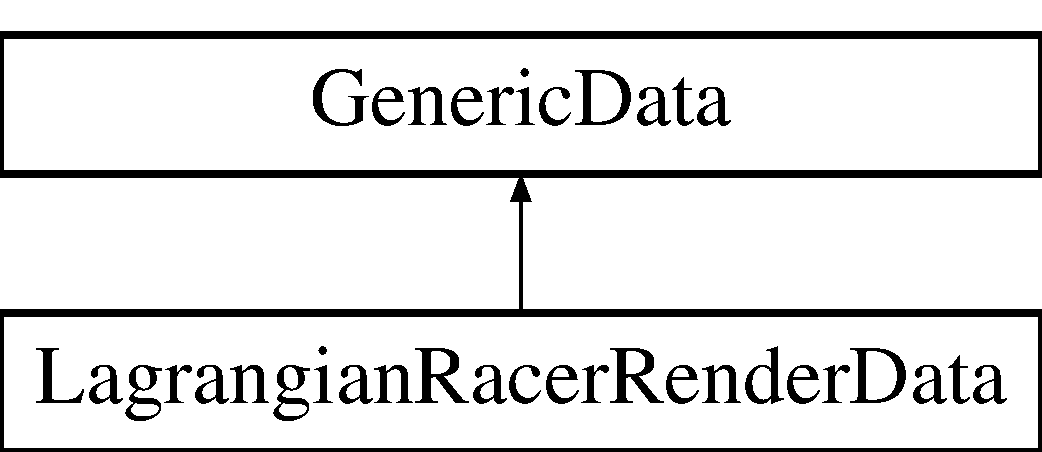
\includegraphics[height=2.000000cm]{class_lagrangian_racer_render_data}
\end{center}
\end{figure}
\subsection*{Public Member Functions}
\begin{DoxyCompactItemize}
\item 
\hyperlink{class_lagrangian_racer_render_data_a727934cebfd0e7ef204f2a038be8ff23}{Lagrangian\-Racer\-Render\-Data} (std\-::string filename)
\item 
\hyperlink{class_lagrangian_racer_render_data_aae7fd9c0acf817800ce3875a81ef2ccb}{Lagrangian\-Racer\-Render\-Data} ()
\item 
\hyperlink{class_lagrangian_racer_render_data_a5c816ec06dc4e39b060eaad063e74d58}{$\sim$\-Lagrangian\-Racer\-Render\-Data} ()
\item 
virtual void \hyperlink{class_lagrangian_racer_render_data_a5df4617924f398cd1bf7c0fd633e8020}{write} (std\-::ostream \&out) const 
\item 
virtual void \hyperlink{class_lagrangian_racer_render_data_aa5174615686e62f00cf5d71ff870e5ca}{read} (std\-::istream \&in)
\end{DoxyCompactItemize}
\subsection*{Public Attributes}
\begin{DoxyCompactItemize}
\item 
double \hyperlink{class_lagrangian_racer_render_data_a766230be72d938b14f4d32b8873092d7}{m\-Hat\-Num\-Textures\-Theta}
\item 
double \hyperlink{class_lagrangian_racer_render_data_a89916f65f2bc1eeab2c65305f0a62409}{m\-Hat\-Num\-Textures\-Z}
\item 
double \hyperlink{class_lagrangian_racer_render_data_ab52e4df8e723b61a488a2768eac88b01}{m\-Head\-Num\-Textures\-Theta}
\item 
double \hyperlink{class_lagrangian_racer_render_data_abe81dcbd66023cef6700fbbce1ffbb66}{m\-Head\-Num\-Textures\-Phi}
\item 
double \hyperlink{class_lagrangian_racer_render_data_a8eedbec1f6341500ed483a4cbc32263f}{m\-Body\-Num\-Textures\-Theta}
\item 
double \hyperlink{class_lagrangian_racer_render_data_a4ac17fa4204b5b45e7c4573fab47e0f1}{m\-Body\-Num\-Textures\-Z}
\item 
double \hyperlink{class_lagrangian_racer_render_data_a3c094864539464ee55ac1cd1a23a0219}{m\-Bottom\-Num\-Textures\-Theta}
\item 
double \hyperlink{class_lagrangian_racer_render_data_acdc57178e2512e9ce095d04694d4db87}{m\-Bottom\-Num\-Textures\-Phi}
\item 
std\-::string \hyperlink{class_lagrangian_racer_render_data_a75dd9e75e88e56ca54635f1db909f12f}{m\-Hat\-Texture\-Filename}
\item 
std\-::string \hyperlink{class_lagrangian_racer_render_data_a7fc760725ac25aadfaf58ef4509a62a6}{m\-Head\-Texture\-Filename}
\item 
std\-::string \hyperlink{class_lagrangian_racer_render_data_a4623ba2adca25658d15e7fd82bb4d7d9}{m\-Body\-Texture\-Filename}
\item 
std\-::string \hyperlink{class_lagrangian_racer_render_data_a2c0d76f2379454fd940c0d6f3382cc57}{m\-Bottom\-Texture\-Filename}
\item 
\hyperlink{class_electric_material_data}{Electric\-Material\-Data} \hyperlink{class_lagrangian_racer_render_data_a6d82009be8fdd7688e4560d98cdc41af}{m\-Hat\-Material}
\item 
\hyperlink{class_electric_material_data}{Electric\-Material\-Data} \hyperlink{class_lagrangian_racer_render_data_acbcdead066f265a07ef25a89459a7f06}{m\-Head\-Material}
\item 
\hyperlink{class_electric_material_data}{Electric\-Material\-Data} \hyperlink{class_lagrangian_racer_render_data_aaa522cfd401f27b708a45d1447b0a28f}{m\-Body\-Material}
\item 
\hyperlink{class_electric_material_data}{Electric\-Material\-Data} \hyperlink{class_lagrangian_racer_render_data_a097eaa5144f9f3a43effd0d1901e9bb5}{m\-Bottom\-Material}
\end{DoxyCompactItemize}


\subsection{Constructor \& Destructor Documentation}
\hypertarget{class_lagrangian_racer_render_data_a727934cebfd0e7ef204f2a038be8ff23}{\index{Lagrangian\-Racer\-Render\-Data@{Lagrangian\-Racer\-Render\-Data}!Lagrangian\-Racer\-Render\-Data@{Lagrangian\-Racer\-Render\-Data}}
\index{Lagrangian\-Racer\-Render\-Data@{Lagrangian\-Racer\-Render\-Data}!LagrangianRacerRenderData@{Lagrangian\-Racer\-Render\-Data}}
\subsubsection[{Lagrangian\-Racer\-Render\-Data}]{\setlength{\rightskip}{0pt plus 5cm}Lagrangian\-Racer\-Render\-Data\-::\-Lagrangian\-Racer\-Render\-Data (
\begin{DoxyParamCaption}
\item[{std\-::string}]{filename}
\end{DoxyParamCaption}
)}}\label{class_lagrangian_racer_render_data_a727934cebfd0e7ef204f2a038be8ff23}
\hypertarget{class_lagrangian_racer_render_data_aae7fd9c0acf817800ce3875a81ef2ccb}{\index{Lagrangian\-Racer\-Render\-Data@{Lagrangian\-Racer\-Render\-Data}!Lagrangian\-Racer\-Render\-Data@{Lagrangian\-Racer\-Render\-Data}}
\index{Lagrangian\-Racer\-Render\-Data@{Lagrangian\-Racer\-Render\-Data}!LagrangianRacerRenderData@{Lagrangian\-Racer\-Render\-Data}}
\subsubsection[{Lagrangian\-Racer\-Render\-Data}]{\setlength{\rightskip}{0pt plus 5cm}Lagrangian\-Racer\-Render\-Data\-::\-Lagrangian\-Racer\-Render\-Data (
\begin{DoxyParamCaption}
{}
\end{DoxyParamCaption}
)}}\label{class_lagrangian_racer_render_data_aae7fd9c0acf817800ce3875a81ef2ccb}
\hypertarget{class_lagrangian_racer_render_data_a5c816ec06dc4e39b060eaad063e74d58}{\index{Lagrangian\-Racer\-Render\-Data@{Lagrangian\-Racer\-Render\-Data}!$\sim$\-Lagrangian\-Racer\-Render\-Data@{$\sim$\-Lagrangian\-Racer\-Render\-Data}}
\index{$\sim$\-Lagrangian\-Racer\-Render\-Data@{$\sim$\-Lagrangian\-Racer\-Render\-Data}!LagrangianRacerRenderData@{Lagrangian\-Racer\-Render\-Data}}
\subsubsection[{$\sim$\-Lagrangian\-Racer\-Render\-Data}]{\setlength{\rightskip}{0pt plus 5cm}Lagrangian\-Racer\-Render\-Data\-::$\sim$\-Lagrangian\-Racer\-Render\-Data (
\begin{DoxyParamCaption}
{}
\end{DoxyParamCaption}
)}}\label{class_lagrangian_racer_render_data_a5c816ec06dc4e39b060eaad063e74d58}


\subsection{Member Function Documentation}
\hypertarget{class_lagrangian_racer_render_data_aa5174615686e62f00cf5d71ff870e5ca}{\index{Lagrangian\-Racer\-Render\-Data@{Lagrangian\-Racer\-Render\-Data}!read@{read}}
\index{read@{read}!LagrangianRacerRenderData@{Lagrangian\-Racer\-Render\-Data}}
\subsubsection[{read}]{\setlength{\rightskip}{0pt plus 5cm}void Lagrangian\-Racer\-Render\-Data\-::read (
\begin{DoxyParamCaption}
\item[{std\-::istream \&}]{in}
\end{DoxyParamCaption}
)\hspace{0.3cm}{\ttfamily [virtual]}}}\label{class_lagrangian_racer_render_data_aa5174615686e62f00cf5d71ff870e5ca}


Implements \hyperlink{class_generic_data_a71e231ef04c9a91a3429123dab5bd1e7}{Generic\-Data}.

\hypertarget{class_lagrangian_racer_render_data_a5df4617924f398cd1bf7c0fd633e8020}{\index{Lagrangian\-Racer\-Render\-Data@{Lagrangian\-Racer\-Render\-Data}!write@{write}}
\index{write@{write}!LagrangianRacerRenderData@{Lagrangian\-Racer\-Render\-Data}}
\subsubsection[{write}]{\setlength{\rightskip}{0pt plus 5cm}void Lagrangian\-Racer\-Render\-Data\-::write (
\begin{DoxyParamCaption}
\item[{std\-::ostream \&}]{out}
\end{DoxyParamCaption}
) const\hspace{0.3cm}{\ttfamily [virtual]}}}\label{class_lagrangian_racer_render_data_a5df4617924f398cd1bf7c0fd633e8020}


Implements \hyperlink{class_generic_data_a93ea61de5b09cf3fc95564ef3d841214}{Generic\-Data}.



\subsection{Member Data Documentation}
\hypertarget{class_lagrangian_racer_render_data_aaa522cfd401f27b708a45d1447b0a28f}{\index{Lagrangian\-Racer\-Render\-Data@{Lagrangian\-Racer\-Render\-Data}!m\-Body\-Material@{m\-Body\-Material}}
\index{m\-Body\-Material@{m\-Body\-Material}!LagrangianRacerRenderData@{Lagrangian\-Racer\-Render\-Data}}
\subsubsection[{m\-Body\-Material}]{\setlength{\rightskip}{0pt plus 5cm}{\bf Electric\-Material\-Data} Lagrangian\-Racer\-Render\-Data\-::m\-Body\-Material}}\label{class_lagrangian_racer_render_data_aaa522cfd401f27b708a45d1447b0a28f}
\hypertarget{class_lagrangian_racer_render_data_a8eedbec1f6341500ed483a4cbc32263f}{\index{Lagrangian\-Racer\-Render\-Data@{Lagrangian\-Racer\-Render\-Data}!m\-Body\-Num\-Textures\-Theta@{m\-Body\-Num\-Textures\-Theta}}
\index{m\-Body\-Num\-Textures\-Theta@{m\-Body\-Num\-Textures\-Theta}!LagrangianRacerRenderData@{Lagrangian\-Racer\-Render\-Data}}
\subsubsection[{m\-Body\-Num\-Textures\-Theta}]{\setlength{\rightskip}{0pt plus 5cm}double Lagrangian\-Racer\-Render\-Data\-::m\-Body\-Num\-Textures\-Theta}}\label{class_lagrangian_racer_render_data_a8eedbec1f6341500ed483a4cbc32263f}
\hypertarget{class_lagrangian_racer_render_data_a4ac17fa4204b5b45e7c4573fab47e0f1}{\index{Lagrangian\-Racer\-Render\-Data@{Lagrangian\-Racer\-Render\-Data}!m\-Body\-Num\-Textures\-Z@{m\-Body\-Num\-Textures\-Z}}
\index{m\-Body\-Num\-Textures\-Z@{m\-Body\-Num\-Textures\-Z}!LagrangianRacerRenderData@{Lagrangian\-Racer\-Render\-Data}}
\subsubsection[{m\-Body\-Num\-Textures\-Z}]{\setlength{\rightskip}{0pt plus 5cm}double Lagrangian\-Racer\-Render\-Data\-::m\-Body\-Num\-Textures\-Z}}\label{class_lagrangian_racer_render_data_a4ac17fa4204b5b45e7c4573fab47e0f1}
\hypertarget{class_lagrangian_racer_render_data_a4623ba2adca25658d15e7fd82bb4d7d9}{\index{Lagrangian\-Racer\-Render\-Data@{Lagrangian\-Racer\-Render\-Data}!m\-Body\-Texture\-Filename@{m\-Body\-Texture\-Filename}}
\index{m\-Body\-Texture\-Filename@{m\-Body\-Texture\-Filename}!LagrangianRacerRenderData@{Lagrangian\-Racer\-Render\-Data}}
\subsubsection[{m\-Body\-Texture\-Filename}]{\setlength{\rightskip}{0pt plus 5cm}std\-::string Lagrangian\-Racer\-Render\-Data\-::m\-Body\-Texture\-Filename}}\label{class_lagrangian_racer_render_data_a4623ba2adca25658d15e7fd82bb4d7d9}
\hypertarget{class_lagrangian_racer_render_data_a097eaa5144f9f3a43effd0d1901e9bb5}{\index{Lagrangian\-Racer\-Render\-Data@{Lagrangian\-Racer\-Render\-Data}!m\-Bottom\-Material@{m\-Bottom\-Material}}
\index{m\-Bottom\-Material@{m\-Bottom\-Material}!LagrangianRacerRenderData@{Lagrangian\-Racer\-Render\-Data}}
\subsubsection[{m\-Bottom\-Material}]{\setlength{\rightskip}{0pt plus 5cm}{\bf Electric\-Material\-Data} Lagrangian\-Racer\-Render\-Data\-::m\-Bottom\-Material}}\label{class_lagrangian_racer_render_data_a097eaa5144f9f3a43effd0d1901e9bb5}
\hypertarget{class_lagrangian_racer_render_data_acdc57178e2512e9ce095d04694d4db87}{\index{Lagrangian\-Racer\-Render\-Data@{Lagrangian\-Racer\-Render\-Data}!m\-Bottom\-Num\-Textures\-Phi@{m\-Bottom\-Num\-Textures\-Phi}}
\index{m\-Bottom\-Num\-Textures\-Phi@{m\-Bottom\-Num\-Textures\-Phi}!LagrangianRacerRenderData@{Lagrangian\-Racer\-Render\-Data}}
\subsubsection[{m\-Bottom\-Num\-Textures\-Phi}]{\setlength{\rightskip}{0pt plus 5cm}double Lagrangian\-Racer\-Render\-Data\-::m\-Bottom\-Num\-Textures\-Phi}}\label{class_lagrangian_racer_render_data_acdc57178e2512e9ce095d04694d4db87}
\hypertarget{class_lagrangian_racer_render_data_a3c094864539464ee55ac1cd1a23a0219}{\index{Lagrangian\-Racer\-Render\-Data@{Lagrangian\-Racer\-Render\-Data}!m\-Bottom\-Num\-Textures\-Theta@{m\-Bottom\-Num\-Textures\-Theta}}
\index{m\-Bottom\-Num\-Textures\-Theta@{m\-Bottom\-Num\-Textures\-Theta}!LagrangianRacerRenderData@{Lagrangian\-Racer\-Render\-Data}}
\subsubsection[{m\-Bottom\-Num\-Textures\-Theta}]{\setlength{\rightskip}{0pt plus 5cm}double Lagrangian\-Racer\-Render\-Data\-::m\-Bottom\-Num\-Textures\-Theta}}\label{class_lagrangian_racer_render_data_a3c094864539464ee55ac1cd1a23a0219}
\hypertarget{class_lagrangian_racer_render_data_a2c0d76f2379454fd940c0d6f3382cc57}{\index{Lagrangian\-Racer\-Render\-Data@{Lagrangian\-Racer\-Render\-Data}!m\-Bottom\-Texture\-Filename@{m\-Bottom\-Texture\-Filename}}
\index{m\-Bottom\-Texture\-Filename@{m\-Bottom\-Texture\-Filename}!LagrangianRacerRenderData@{Lagrangian\-Racer\-Render\-Data}}
\subsubsection[{m\-Bottom\-Texture\-Filename}]{\setlength{\rightskip}{0pt plus 5cm}std\-::string Lagrangian\-Racer\-Render\-Data\-::m\-Bottom\-Texture\-Filename}}\label{class_lagrangian_racer_render_data_a2c0d76f2379454fd940c0d6f3382cc57}
\hypertarget{class_lagrangian_racer_render_data_a6d82009be8fdd7688e4560d98cdc41af}{\index{Lagrangian\-Racer\-Render\-Data@{Lagrangian\-Racer\-Render\-Data}!m\-Hat\-Material@{m\-Hat\-Material}}
\index{m\-Hat\-Material@{m\-Hat\-Material}!LagrangianRacerRenderData@{Lagrangian\-Racer\-Render\-Data}}
\subsubsection[{m\-Hat\-Material}]{\setlength{\rightskip}{0pt plus 5cm}{\bf Electric\-Material\-Data} Lagrangian\-Racer\-Render\-Data\-::m\-Hat\-Material}}\label{class_lagrangian_racer_render_data_a6d82009be8fdd7688e4560d98cdc41af}
\hypertarget{class_lagrangian_racer_render_data_a766230be72d938b14f4d32b8873092d7}{\index{Lagrangian\-Racer\-Render\-Data@{Lagrangian\-Racer\-Render\-Data}!m\-Hat\-Num\-Textures\-Theta@{m\-Hat\-Num\-Textures\-Theta}}
\index{m\-Hat\-Num\-Textures\-Theta@{m\-Hat\-Num\-Textures\-Theta}!LagrangianRacerRenderData@{Lagrangian\-Racer\-Render\-Data}}
\subsubsection[{m\-Hat\-Num\-Textures\-Theta}]{\setlength{\rightskip}{0pt plus 5cm}double Lagrangian\-Racer\-Render\-Data\-::m\-Hat\-Num\-Textures\-Theta}}\label{class_lagrangian_racer_render_data_a766230be72d938b14f4d32b8873092d7}
\hypertarget{class_lagrangian_racer_render_data_a89916f65f2bc1eeab2c65305f0a62409}{\index{Lagrangian\-Racer\-Render\-Data@{Lagrangian\-Racer\-Render\-Data}!m\-Hat\-Num\-Textures\-Z@{m\-Hat\-Num\-Textures\-Z}}
\index{m\-Hat\-Num\-Textures\-Z@{m\-Hat\-Num\-Textures\-Z}!LagrangianRacerRenderData@{Lagrangian\-Racer\-Render\-Data}}
\subsubsection[{m\-Hat\-Num\-Textures\-Z}]{\setlength{\rightskip}{0pt plus 5cm}double Lagrangian\-Racer\-Render\-Data\-::m\-Hat\-Num\-Textures\-Z}}\label{class_lagrangian_racer_render_data_a89916f65f2bc1eeab2c65305f0a62409}
\hypertarget{class_lagrangian_racer_render_data_a75dd9e75e88e56ca54635f1db909f12f}{\index{Lagrangian\-Racer\-Render\-Data@{Lagrangian\-Racer\-Render\-Data}!m\-Hat\-Texture\-Filename@{m\-Hat\-Texture\-Filename}}
\index{m\-Hat\-Texture\-Filename@{m\-Hat\-Texture\-Filename}!LagrangianRacerRenderData@{Lagrangian\-Racer\-Render\-Data}}
\subsubsection[{m\-Hat\-Texture\-Filename}]{\setlength{\rightskip}{0pt plus 5cm}std\-::string Lagrangian\-Racer\-Render\-Data\-::m\-Hat\-Texture\-Filename}}\label{class_lagrangian_racer_render_data_a75dd9e75e88e56ca54635f1db909f12f}
\hypertarget{class_lagrangian_racer_render_data_acbcdead066f265a07ef25a89459a7f06}{\index{Lagrangian\-Racer\-Render\-Data@{Lagrangian\-Racer\-Render\-Data}!m\-Head\-Material@{m\-Head\-Material}}
\index{m\-Head\-Material@{m\-Head\-Material}!LagrangianRacerRenderData@{Lagrangian\-Racer\-Render\-Data}}
\subsubsection[{m\-Head\-Material}]{\setlength{\rightskip}{0pt plus 5cm}{\bf Electric\-Material\-Data} Lagrangian\-Racer\-Render\-Data\-::m\-Head\-Material}}\label{class_lagrangian_racer_render_data_acbcdead066f265a07ef25a89459a7f06}
\hypertarget{class_lagrangian_racer_render_data_abe81dcbd66023cef6700fbbce1ffbb66}{\index{Lagrangian\-Racer\-Render\-Data@{Lagrangian\-Racer\-Render\-Data}!m\-Head\-Num\-Textures\-Phi@{m\-Head\-Num\-Textures\-Phi}}
\index{m\-Head\-Num\-Textures\-Phi@{m\-Head\-Num\-Textures\-Phi}!LagrangianRacerRenderData@{Lagrangian\-Racer\-Render\-Data}}
\subsubsection[{m\-Head\-Num\-Textures\-Phi}]{\setlength{\rightskip}{0pt plus 5cm}double Lagrangian\-Racer\-Render\-Data\-::m\-Head\-Num\-Textures\-Phi}}\label{class_lagrangian_racer_render_data_abe81dcbd66023cef6700fbbce1ffbb66}
\hypertarget{class_lagrangian_racer_render_data_ab52e4df8e723b61a488a2768eac88b01}{\index{Lagrangian\-Racer\-Render\-Data@{Lagrangian\-Racer\-Render\-Data}!m\-Head\-Num\-Textures\-Theta@{m\-Head\-Num\-Textures\-Theta}}
\index{m\-Head\-Num\-Textures\-Theta@{m\-Head\-Num\-Textures\-Theta}!LagrangianRacerRenderData@{Lagrangian\-Racer\-Render\-Data}}
\subsubsection[{m\-Head\-Num\-Textures\-Theta}]{\setlength{\rightskip}{0pt plus 5cm}double Lagrangian\-Racer\-Render\-Data\-::m\-Head\-Num\-Textures\-Theta}}\label{class_lagrangian_racer_render_data_ab52e4df8e723b61a488a2768eac88b01}
\hypertarget{class_lagrangian_racer_render_data_a7fc760725ac25aadfaf58ef4509a62a6}{\index{Lagrangian\-Racer\-Render\-Data@{Lagrangian\-Racer\-Render\-Data}!m\-Head\-Texture\-Filename@{m\-Head\-Texture\-Filename}}
\index{m\-Head\-Texture\-Filename@{m\-Head\-Texture\-Filename}!LagrangianRacerRenderData@{Lagrangian\-Racer\-Render\-Data}}
\subsubsection[{m\-Head\-Texture\-Filename}]{\setlength{\rightskip}{0pt plus 5cm}std\-::string Lagrangian\-Racer\-Render\-Data\-::m\-Head\-Texture\-Filename}}\label{class_lagrangian_racer_render_data_a7fc760725ac25aadfaf58ef4509a62a6}


The documentation for this class was generated from the following files\-:\begin{DoxyCompactItemize}
\item 
C\-:/\-Users/\-Owner/\-My Programming/\-Personal Projects/\-Video\-Games/\-Optimist Racing/src/\hyperlink{_data_8hpp}{Data.\-hpp}\item 
C\-:/\-Users/\-Owner/\-My Programming/\-Personal Projects/\-Video\-Games/\-Optimist Racing/src/\hyperlink{_data_8cpp}{Data.\-cpp}\end{DoxyCompactItemize}

\hypertarget{class_lagrange_1_1_lagrangian_racer_system}{\section{Lagrange\-:\-:Lagrangian\-Racer\-System Class Reference}
\label{class_lagrange_1_1_lagrangian_racer_system}\index{Lagrange\-::\-Lagrangian\-Racer\-System@{Lagrange\-::\-Lagrangian\-Racer\-System}}
}


{\ttfamily \#include $<$Lagrange.\-hpp$>$}

Inheritance diagram for Lagrange\-:\-:Lagrangian\-Racer\-System\-:\begin{figure}[H]
\begin{center}
\leavevmode
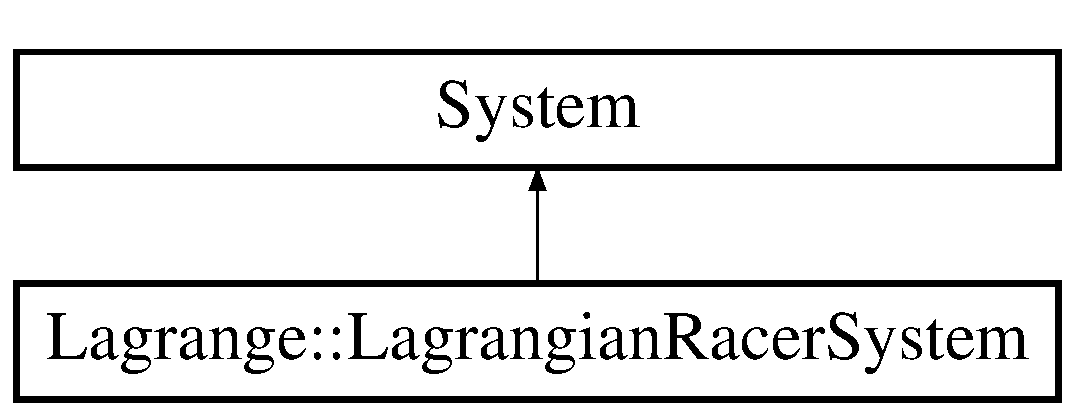
\includegraphics[height=2.000000cm]{class_lagrange_1_1_lagrangian_racer_system}
\end{center}
\end{figure}
\subsection*{Additional Inherited Members}


The documentation for this class was generated from the following file\-:\begin{DoxyCompactItemize}
\item 
C\-:/\-Users/\-Owner/\-My Programming/\-Personal Projects/\-Video\-Games/\-Optimist Racing/src/\hyperlink{_lagrange_8hpp}{Lagrange.\-hpp}\end{DoxyCompactItemize}

\hypertarget{class_material}{\section{Material Class Reference}
\label{class_material}\index{Material@{Material}}
}


{\ttfamily \#include $<$Material.\-hpp$>$}

\subsection*{Public Member Functions}
\begin{DoxyCompactItemize}
\item 
\hyperlink{class_material_a9954425c47f571d50799273c360fb464}{Material} (\hyperlink{class_colour}{Colour} emission, \hyperlink{class_colour}{Colour} ambient, \hyperlink{class_colour}{Colour} diffuse, \hyperlink{class_colour}{Colour} specular, double shininess)
\item 
\hyperlink{class_material_a2c19452d71f54075df8f5405b03129f4}{$\sim$\-Material} ()
\item 
void \hyperlink{class_material_a60f350c5747dc9a65ad326ca8e69db3a}{gl\-Apply} (G\-Lenum face) const 
\end{DoxyCompactItemize}


\subsection{Constructor \& Destructor Documentation}
\hypertarget{class_material_a9954425c47f571d50799273c360fb464}{\index{Material@{Material}!Material@{Material}}
\index{Material@{Material}!Material@{Material}}
\subsubsection[{Material}]{\setlength{\rightskip}{0pt plus 5cm}Material\-::\-Material (
\begin{DoxyParamCaption}
\item[{{\bf Colour}}]{emission, }
\item[{{\bf Colour}}]{ambient, }
\item[{{\bf Colour}}]{diffuse, }
\item[{{\bf Colour}}]{specular, }
\item[{double}]{shininess}
\end{DoxyParamCaption}
)}}\label{class_material_a9954425c47f571d50799273c360fb464}
\hypertarget{class_material_a2c19452d71f54075df8f5405b03129f4}{\index{Material@{Material}!$\sim$\-Material@{$\sim$\-Material}}
\index{$\sim$\-Material@{$\sim$\-Material}!Material@{Material}}
\subsubsection[{$\sim$\-Material}]{\setlength{\rightskip}{0pt plus 5cm}Material\-::$\sim$\-Material (
\begin{DoxyParamCaption}
{}
\end{DoxyParamCaption}
)}}\label{class_material_a2c19452d71f54075df8f5405b03129f4}


\subsection{Member Function Documentation}
\hypertarget{class_material_a60f350c5747dc9a65ad326ca8e69db3a}{\index{Material@{Material}!gl\-Apply@{gl\-Apply}}
\index{gl\-Apply@{gl\-Apply}!Material@{Material}}
\subsubsection[{gl\-Apply}]{\setlength{\rightskip}{0pt plus 5cm}void Material\-::gl\-Apply (
\begin{DoxyParamCaption}
\item[{G\-Lenum}]{face}
\end{DoxyParamCaption}
) const}}\label{class_material_a60f350c5747dc9a65ad326ca8e69db3a}


The documentation for this class was generated from the following files\-:\begin{DoxyCompactItemize}
\item 
C\-:/\-Users/\-Owner/\-My Programming/\-Personal Projects/\-Video\-Games/\-Optimist Racing/src/\hyperlink{_material_8hpp}{Material.\-hpp}\item 
C\-:/\-Users/\-Owner/\-My Programming/\-Personal Projects/\-Video\-Games/\-Optimist Racing/src/\hyperlink{_material_8cpp}{Material.\-cpp}\end{DoxyCompactItemize}

\hypertarget{struct_matrix1_vector1}{\section{Matrix1\-Vector1 Struct Reference}
\label{struct_matrix1_vector1}\index{Matrix1\-Vector1@{Matrix1\-Vector1}}
}


This struct holds one \hyperlink{class_matrix_mx_n}{Matrix\-Mx\-N} and one \hyperlink{class_vector_n_d}{Vector\-N\-D}.  




{\ttfamily \#include $<$Algebra\-Struct.\-hpp$>$}

\subsection*{Public Member Functions}
\begin{DoxyCompactItemize}
\item 
\hyperlink{struct_matrix1_vector1_ab63968faa92db39b0418ae6f313a25e1}{Matrix1\-Vector1} (const \hyperlink{class_matrix_mx_n}{Matrix\-Mx\-N} \&\hyperlink{struct_matrix1_vector1_ad92f271648e49bf11330c09e48ff474a}{m\-Matrix}, const \hyperlink{class_vector_n_d}{Vector\-N\-D} \&\hyperlink{struct_matrix1_vector1_a6986b2fafa3d34ea4f3ffc614c12eb7e}{m\-Vector})
\begin{DoxyCompactList}\small\item\em The constructor. \end{DoxyCompactList}\end{DoxyCompactItemize}
\subsection*{Public Attributes}
\begin{DoxyCompactItemize}
\item 
const \hyperlink{class_matrix_mx_n}{Matrix\-Mx\-N} \& \hyperlink{struct_matrix1_vector1_ad92f271648e49bf11330c09e48ff474a}{m\-Matrix}
\begin{DoxyCompactList}\small\item\em The matrix. \end{DoxyCompactList}\item 
const \hyperlink{class_vector_n_d}{Vector\-N\-D} \& \hyperlink{struct_matrix1_vector1_a6986b2fafa3d34ea4f3ffc614c12eb7e}{m\-Vector}
\begin{DoxyCompactList}\small\item\em The vector. \end{DoxyCompactList}\end{DoxyCompactItemize}


\subsection{Detailed Description}
This struct holds one \hyperlink{class_matrix_mx_n}{Matrix\-Mx\-N} and one \hyperlink{class_vector_n_d}{Vector\-N\-D}. 

\subsection{Constructor \& Destructor Documentation}
\hypertarget{struct_matrix1_vector1_ab63968faa92db39b0418ae6f313a25e1}{\index{Matrix1\-Vector1@{Matrix1\-Vector1}!Matrix1\-Vector1@{Matrix1\-Vector1}}
\index{Matrix1\-Vector1@{Matrix1\-Vector1}!Matrix1Vector1@{Matrix1\-Vector1}}
\subsubsection[{Matrix1\-Vector1}]{\setlength{\rightskip}{0pt plus 5cm}Matrix1\-Vector1\-::\-Matrix1\-Vector1 (
\begin{DoxyParamCaption}
\item[{const {\bf Matrix\-Mx\-N} \&}]{m\-Matrix, }
\item[{const {\bf Vector\-N\-D} \&}]{m\-Vector}
\end{DoxyParamCaption}
)}}\label{struct_matrix1_vector1_ab63968faa92db39b0418ae6f313a25e1}


The constructor. 



\subsection{Member Data Documentation}
\hypertarget{struct_matrix1_vector1_ad92f271648e49bf11330c09e48ff474a}{\index{Matrix1\-Vector1@{Matrix1\-Vector1}!m\-Matrix@{m\-Matrix}}
\index{m\-Matrix@{m\-Matrix}!Matrix1Vector1@{Matrix1\-Vector1}}
\subsubsection[{m\-Matrix}]{\setlength{\rightskip}{0pt plus 5cm}const {\bf Matrix\-Mx\-N}\& Matrix1\-Vector1\-::m\-Matrix}}\label{struct_matrix1_vector1_ad92f271648e49bf11330c09e48ff474a}


The matrix. 

\hypertarget{struct_matrix1_vector1_a6986b2fafa3d34ea4f3ffc614c12eb7e}{\index{Matrix1\-Vector1@{Matrix1\-Vector1}!m\-Vector@{m\-Vector}}
\index{m\-Vector@{m\-Vector}!Matrix1Vector1@{Matrix1\-Vector1}}
\subsubsection[{m\-Vector}]{\setlength{\rightskip}{0pt plus 5cm}const {\bf Vector\-N\-D}\& Matrix1\-Vector1\-::m\-Vector}}\label{struct_matrix1_vector1_a6986b2fafa3d34ea4f3ffc614c12eb7e}


The vector. 



The documentation for this struct was generated from the following file\-:\begin{DoxyCompactItemize}
\item 
C\-:/\-Users/\-Owner/\-My Programming/\-Personal Projects/\-Video\-Games/\-Optimist Racing/src/\hyperlink{_algebra_struct_8hpp}{Algebra\-Struct.\-hpp}\end{DoxyCompactItemize}

\hypertarget{class_matrix2x2}{\section{Matrix2x2 Class Reference}
\label{class_matrix2x2}\index{Matrix2x2@{Matrix2x2}}
}


{\ttfamily \#include $<$Algebra.\-hpp$>$}

\subsection*{Public Member Functions}
\begin{DoxyCompactItemize}
\item 
\hyperlink{class_matrix2x2_aca3f61a3a1bce86fd10f3e8b70f70e81}{Matrix2x2} ()
\item 
\hyperlink{class_matrix2x2_ace1cda72cf042dd31876c0d059c9e9bf}{Matrix2x2} (const \hyperlink{class_matrix2x2}{Matrix2x2} \&other)
\item 
\hyperlink{class_matrix2x2_a001283eaf70db2e8f935ef103b3fe98e}{Matrix2x2} (const \hyperlink{class_vector2_d}{Vector2\-D} \&row1, const \hyperlink{class_vector2_d}{Vector2\-D} \&row2)
\item 
\hyperlink{class_matrix2x2_af05682ae3b80edd3b14ac43db5ef0c08}{Matrix2x2} (const double $\ast$values)
\item 
\hyperlink{class_matrix2x2}{Matrix2x2} \& \hyperlink{class_matrix2x2_af1e1812c8ecd1f5fe0de70780e996b53}{operator=} (const \hyperlink{class_matrix2x2}{Matrix2x2} \&other)
\item 
\hyperlink{class_vector2_d}{Vector2\-D} \hyperlink{class_matrix2x2_a3a03aae0dde8aaf2579bbead6e58c25a}{get\-Row} (size\-\_\-t row) const 
\item 
double $\ast$ \hyperlink{class_matrix2x2_a72cd1d0d3fc8876b6a17632079c45227}{get\-Row} (size\-\_\-t row)
\item 
\hyperlink{class_vector2_d}{Vector2\-D} \hyperlink{class_matrix2x2_a299ddc8aba2c00d3e61071ac8261b17a}{get\-Column} (size\-\_\-t col) const 
\item 
\hyperlink{class_vector2_d}{Vector2\-D} \hyperlink{class_matrix2x2_a83296205a183d5ab07aa6b4947c16bf2}{operator\mbox{[}$\,$\mbox{]}} (size\-\_\-t row) const 
\item 
double $\ast$ \hyperlink{class_matrix2x2_a6e607183b40dd89bb123971a09f99f91}{operator\mbox{[}$\,$\mbox{]}} (size\-\_\-t row)
\item 
\hyperlink{class_matrix2x2}{Matrix2x2} \hyperlink{class_matrix2x2_a7630ef26f2a09c33137b680a468a114b}{transpose} () const 
\item 
\hyperlink{class_matrix2x2}{Matrix2x2} \hyperlink{class_matrix2x2_a5c4d3f6f5ba43791cad0fd210886c0d6}{invert} () const 
\item 
double \hyperlink{class_matrix2x2_a4498d52afa9436548e98105ac39f995a}{determinant} () const 
\item 
\hyperlink{class_vector2_d}{Vector2\-D} \hyperlink{class_matrix2x2_aa0c530a9fe1db1065a39af880ddbaca9}{matrix\-Solve} (const \hyperlink{class_vector2_d}{Vector2\-D} \&b) const 
\item 
const double $\ast$ \hyperlink{class_matrix2x2_a7bdbb1745aae6fa25060c9db113f0fea}{begin} () const 
\item 
const double $\ast$ \hyperlink{class_matrix2x2_a763a2edfa907e05301e46f8864921bfe}{end} () const 
\end{DoxyCompactItemize}


\subsection{Constructor \& Destructor Documentation}
\hypertarget{class_matrix2x2_aca3f61a3a1bce86fd10f3e8b70f70e81}{\index{Matrix2x2@{Matrix2x2}!Matrix2x2@{Matrix2x2}}
\index{Matrix2x2@{Matrix2x2}!Matrix2x2@{Matrix2x2}}
\subsubsection[{Matrix2x2}]{\setlength{\rightskip}{0pt plus 5cm}Matrix2x2\-::\-Matrix2x2 (
\begin{DoxyParamCaption}
{}
\end{DoxyParamCaption}
)}}\label{class_matrix2x2_aca3f61a3a1bce86fd10f3e8b70f70e81}
\hypertarget{class_matrix2x2_ace1cda72cf042dd31876c0d059c9e9bf}{\index{Matrix2x2@{Matrix2x2}!Matrix2x2@{Matrix2x2}}
\index{Matrix2x2@{Matrix2x2}!Matrix2x2@{Matrix2x2}}
\subsubsection[{Matrix2x2}]{\setlength{\rightskip}{0pt plus 5cm}Matrix2x2\-::\-Matrix2x2 (
\begin{DoxyParamCaption}
\item[{const {\bf Matrix2x2} \&}]{other}
\end{DoxyParamCaption}
)}}\label{class_matrix2x2_ace1cda72cf042dd31876c0d059c9e9bf}
\hypertarget{class_matrix2x2_a001283eaf70db2e8f935ef103b3fe98e}{\index{Matrix2x2@{Matrix2x2}!Matrix2x2@{Matrix2x2}}
\index{Matrix2x2@{Matrix2x2}!Matrix2x2@{Matrix2x2}}
\subsubsection[{Matrix2x2}]{\setlength{\rightskip}{0pt plus 5cm}Matrix2x2\-::\-Matrix2x2 (
\begin{DoxyParamCaption}
\item[{const {\bf Vector2\-D} \&}]{row1, }
\item[{const {\bf Vector2\-D} \&}]{row2}
\end{DoxyParamCaption}
)}}\label{class_matrix2x2_a001283eaf70db2e8f935ef103b3fe98e}
\hypertarget{class_matrix2x2_af05682ae3b80edd3b14ac43db5ef0c08}{\index{Matrix2x2@{Matrix2x2}!Matrix2x2@{Matrix2x2}}
\index{Matrix2x2@{Matrix2x2}!Matrix2x2@{Matrix2x2}}
\subsubsection[{Matrix2x2}]{\setlength{\rightskip}{0pt plus 5cm}Matrix2x2\-::\-Matrix2x2 (
\begin{DoxyParamCaption}
\item[{const double $\ast$}]{values}
\end{DoxyParamCaption}
)}}\label{class_matrix2x2_af05682ae3b80edd3b14ac43db5ef0c08}


\subsection{Member Function Documentation}
\hypertarget{class_matrix2x2_a7bdbb1745aae6fa25060c9db113f0fea}{\index{Matrix2x2@{Matrix2x2}!begin@{begin}}
\index{begin@{begin}!Matrix2x2@{Matrix2x2}}
\subsubsection[{begin}]{\setlength{\rightskip}{0pt plus 5cm}const double $\ast$ Matrix2x2\-::begin (
\begin{DoxyParamCaption}
{}
\end{DoxyParamCaption}
) const}}\label{class_matrix2x2_a7bdbb1745aae6fa25060c9db113f0fea}
\hypertarget{class_matrix2x2_a4498d52afa9436548e98105ac39f995a}{\index{Matrix2x2@{Matrix2x2}!determinant@{determinant}}
\index{determinant@{determinant}!Matrix2x2@{Matrix2x2}}
\subsubsection[{determinant}]{\setlength{\rightskip}{0pt plus 5cm}double Matrix2x2\-::determinant (
\begin{DoxyParamCaption}
{}
\end{DoxyParamCaption}
) const}}\label{class_matrix2x2_a4498d52afa9436548e98105ac39f995a}
\hypertarget{class_matrix2x2_a763a2edfa907e05301e46f8864921bfe}{\index{Matrix2x2@{Matrix2x2}!end@{end}}
\index{end@{end}!Matrix2x2@{Matrix2x2}}
\subsubsection[{end}]{\setlength{\rightskip}{0pt plus 5cm}const double $\ast$ Matrix2x2\-::end (
\begin{DoxyParamCaption}
{}
\end{DoxyParamCaption}
) const}}\label{class_matrix2x2_a763a2edfa907e05301e46f8864921bfe}
\hypertarget{class_matrix2x2_a299ddc8aba2c00d3e61071ac8261b17a}{\index{Matrix2x2@{Matrix2x2}!get\-Column@{get\-Column}}
\index{get\-Column@{get\-Column}!Matrix2x2@{Matrix2x2}}
\subsubsection[{get\-Column}]{\setlength{\rightskip}{0pt plus 5cm}{\bf Vector2\-D} Matrix2x2\-::get\-Column (
\begin{DoxyParamCaption}
\item[{size\-\_\-t}]{col}
\end{DoxyParamCaption}
) const}}\label{class_matrix2x2_a299ddc8aba2c00d3e61071ac8261b17a}
\hypertarget{class_matrix2x2_a3a03aae0dde8aaf2579bbead6e58c25a}{\index{Matrix2x2@{Matrix2x2}!get\-Row@{get\-Row}}
\index{get\-Row@{get\-Row}!Matrix2x2@{Matrix2x2}}
\subsubsection[{get\-Row}]{\setlength{\rightskip}{0pt plus 5cm}{\bf Vector2\-D} Matrix2x2\-::get\-Row (
\begin{DoxyParamCaption}
\item[{size\-\_\-t}]{row}
\end{DoxyParamCaption}
) const}}\label{class_matrix2x2_a3a03aae0dde8aaf2579bbead6e58c25a}
\hypertarget{class_matrix2x2_a72cd1d0d3fc8876b6a17632079c45227}{\index{Matrix2x2@{Matrix2x2}!get\-Row@{get\-Row}}
\index{get\-Row@{get\-Row}!Matrix2x2@{Matrix2x2}}
\subsubsection[{get\-Row}]{\setlength{\rightskip}{0pt plus 5cm}double $\ast$ Matrix2x2\-::get\-Row (
\begin{DoxyParamCaption}
\item[{size\-\_\-t}]{row}
\end{DoxyParamCaption}
)}}\label{class_matrix2x2_a72cd1d0d3fc8876b6a17632079c45227}
\hypertarget{class_matrix2x2_a5c4d3f6f5ba43791cad0fd210886c0d6}{\index{Matrix2x2@{Matrix2x2}!invert@{invert}}
\index{invert@{invert}!Matrix2x2@{Matrix2x2}}
\subsubsection[{invert}]{\setlength{\rightskip}{0pt plus 5cm}{\bf Matrix2x2} Matrix2x2\-::invert (
\begin{DoxyParamCaption}
{}
\end{DoxyParamCaption}
) const}}\label{class_matrix2x2_a5c4d3f6f5ba43791cad0fd210886c0d6}
\hypertarget{class_matrix2x2_aa0c530a9fe1db1065a39af880ddbaca9}{\index{Matrix2x2@{Matrix2x2}!matrix\-Solve@{matrix\-Solve}}
\index{matrix\-Solve@{matrix\-Solve}!Matrix2x2@{Matrix2x2}}
\subsubsection[{matrix\-Solve}]{\setlength{\rightskip}{0pt plus 5cm}{\bf Vector2\-D} Matrix2x2\-::matrix\-Solve (
\begin{DoxyParamCaption}
\item[{const {\bf Vector2\-D} \&}]{b}
\end{DoxyParamCaption}
) const}}\label{class_matrix2x2_aa0c530a9fe1db1065a39af880ddbaca9}
\hypertarget{class_matrix2x2_af1e1812c8ecd1f5fe0de70780e996b53}{\index{Matrix2x2@{Matrix2x2}!operator=@{operator=}}
\index{operator=@{operator=}!Matrix2x2@{Matrix2x2}}
\subsubsection[{operator=}]{\setlength{\rightskip}{0pt plus 5cm}{\bf Matrix2x2} \& Matrix2x2\-::operator= (
\begin{DoxyParamCaption}
\item[{const {\bf Matrix2x2} \&}]{other}
\end{DoxyParamCaption}
)}}\label{class_matrix2x2_af1e1812c8ecd1f5fe0de70780e996b53}
\hypertarget{class_matrix2x2_a83296205a183d5ab07aa6b4947c16bf2}{\index{Matrix2x2@{Matrix2x2}!operator\mbox{[}$\,$\mbox{]}@{operator[]}}
\index{operator\mbox{[}$\,$\mbox{]}@{operator[]}!Matrix2x2@{Matrix2x2}}
\subsubsection[{operator[]}]{\setlength{\rightskip}{0pt plus 5cm}{\bf Vector2\-D} Matrix2x2\-::operator\mbox{[}$\,$\mbox{]} (
\begin{DoxyParamCaption}
\item[{size\-\_\-t}]{row}
\end{DoxyParamCaption}
) const}}\label{class_matrix2x2_a83296205a183d5ab07aa6b4947c16bf2}
\hypertarget{class_matrix2x2_a6e607183b40dd89bb123971a09f99f91}{\index{Matrix2x2@{Matrix2x2}!operator\mbox{[}$\,$\mbox{]}@{operator[]}}
\index{operator\mbox{[}$\,$\mbox{]}@{operator[]}!Matrix2x2@{Matrix2x2}}
\subsubsection[{operator[]}]{\setlength{\rightskip}{0pt plus 5cm}double $\ast$ Matrix2x2\-::operator\mbox{[}$\,$\mbox{]} (
\begin{DoxyParamCaption}
\item[{size\-\_\-t}]{row}
\end{DoxyParamCaption}
)}}\label{class_matrix2x2_a6e607183b40dd89bb123971a09f99f91}
\hypertarget{class_matrix2x2_a7630ef26f2a09c33137b680a468a114b}{\index{Matrix2x2@{Matrix2x2}!transpose@{transpose}}
\index{transpose@{transpose}!Matrix2x2@{Matrix2x2}}
\subsubsection[{transpose}]{\setlength{\rightskip}{0pt plus 5cm}{\bf Matrix2x2} Matrix2x2\-::transpose (
\begin{DoxyParamCaption}
{}
\end{DoxyParamCaption}
) const}}\label{class_matrix2x2_a7630ef26f2a09c33137b680a468a114b}


The documentation for this class was generated from the following files\-:\begin{DoxyCompactItemize}
\item 
C\-:/\-Users/\-Owner/\-My Programming/\-Personal Projects/\-Video\-Games/\-Optimist Racing/src/\hyperlink{_algebra_8hpp}{Algebra.\-hpp}\item 
C\-:/\-Users/\-Owner/\-My Programming/\-Personal Projects/\-Video\-Games/\-Optimist Racing/src/\hyperlink{_algebra_8cpp}{Algebra.\-cpp}\end{DoxyCompactItemize}

\hypertarget{class_matrix3x3}{\section{Matrix3x3 Class Reference}
\label{class_matrix3x3}\index{Matrix3x3@{Matrix3x3}}
}


{\ttfamily \#include $<$Algebra.\-hpp$>$}

\subsection*{Public Member Functions}
\begin{DoxyCompactItemize}
\item 
\hyperlink{class_matrix3x3_ac6b901793405c0f36f65d6c4a624d0e7}{Matrix3x3} ()
\item 
\hyperlink{class_matrix3x3_abe38083cf46bb1f783ff64917a9e5404}{Matrix3x3} (const \hyperlink{class_matrix3x3}{Matrix3x3} \&other)
\item 
\hyperlink{class_matrix3x3_a4830a1913f2aa6f9c38281062aaed303}{Matrix3x3} (const \hyperlink{class_vector3_d}{Vector3\-D} \&row1, const \hyperlink{class_vector3_d}{Vector3\-D} \&row2, const \hyperlink{class_vector3_d}{Vector3\-D} \&row3)
\item 
\hyperlink{class_matrix3x3_a77720ea70bf2bb1fae52667aeb3bf419}{Matrix3x3} (const double $\ast$values)
\item 
\hyperlink{class_matrix3x3}{Matrix3x3} \& \hyperlink{class_matrix3x3_ab91b7dc85335166bdc20b77b8f9c34e9}{operator=} (const \hyperlink{class_matrix3x3}{Matrix3x3} \&other)
\item 
\hyperlink{class_vector3_d}{Vector3\-D} \hyperlink{class_matrix3x3_a04888194a52b970549b5fbe40c5a80b3}{get\-Row} (size\-\_\-t row) const 
\item 
double $\ast$ \hyperlink{class_matrix3x3_a9e55dda2c3616c79254429ffbcecc6d4}{get\-Row} (size\-\_\-t row)
\item 
\hyperlink{class_vector3_d}{Vector3\-D} \hyperlink{class_matrix3x3_a3243d4730e65222094e8e7589ded5162}{get\-Column} (size\-\_\-t col) const 
\item 
\hyperlink{class_vector3_d}{Vector3\-D} \hyperlink{class_matrix3x3_a37f611d52839c3790c1983dced8cbf56}{operator\mbox{[}$\,$\mbox{]}} (size\-\_\-t row) const 
\item 
double $\ast$ \hyperlink{class_matrix3x3_a96590caac1fd0d0ba1c344b5cced47eb}{operator\mbox{[}$\,$\mbox{]}} (size\-\_\-t row)
\item 
\hyperlink{class_matrix3x3}{Matrix3x3} \hyperlink{class_matrix3x3_a6d2a2b5c4d1876a72aeada3879dc507b}{transpose} () const 
\item 
\hyperlink{class_matrix3x3}{Matrix3x3} \hyperlink{class_matrix3x3_ac6c35af02989e2a20a0d661d665cc59d}{invert} () const 
\item 
double \hyperlink{class_matrix3x3_a8d069ee838151dfd79fef81a5992bebc}{determinant} () const 
\item 
\hyperlink{class_vector3_d}{Vector3\-D} \hyperlink{class_matrix3x3_a9e92abe88ebfa2f898ea1c3a008d7615}{matrix\-Solve} (const \hyperlink{class_vector3_d}{Vector3\-D} \&b) const 
\item 
const double $\ast$ \hyperlink{class_matrix3x3_ab6a79b3aca663ddb2362ee0639ffed3a}{begin} () const 
\item 
const double $\ast$ \hyperlink{class_matrix3x3_a2a4b6ee9463566d7aed3e1824e08d47e}{end} () const 
\end{DoxyCompactItemize}


\subsection{Constructor \& Destructor Documentation}
\hypertarget{class_matrix3x3_ac6b901793405c0f36f65d6c4a624d0e7}{\index{Matrix3x3@{Matrix3x3}!Matrix3x3@{Matrix3x3}}
\index{Matrix3x3@{Matrix3x3}!Matrix3x3@{Matrix3x3}}
\subsubsection[{Matrix3x3}]{\setlength{\rightskip}{0pt plus 5cm}Matrix3x3\-::\-Matrix3x3 (
\begin{DoxyParamCaption}
{}
\end{DoxyParamCaption}
)}}\label{class_matrix3x3_ac6b901793405c0f36f65d6c4a624d0e7}
\hypertarget{class_matrix3x3_abe38083cf46bb1f783ff64917a9e5404}{\index{Matrix3x3@{Matrix3x3}!Matrix3x3@{Matrix3x3}}
\index{Matrix3x3@{Matrix3x3}!Matrix3x3@{Matrix3x3}}
\subsubsection[{Matrix3x3}]{\setlength{\rightskip}{0pt plus 5cm}Matrix3x3\-::\-Matrix3x3 (
\begin{DoxyParamCaption}
\item[{const {\bf Matrix3x3} \&}]{other}
\end{DoxyParamCaption}
)}}\label{class_matrix3x3_abe38083cf46bb1f783ff64917a9e5404}
\hypertarget{class_matrix3x3_a4830a1913f2aa6f9c38281062aaed303}{\index{Matrix3x3@{Matrix3x3}!Matrix3x3@{Matrix3x3}}
\index{Matrix3x3@{Matrix3x3}!Matrix3x3@{Matrix3x3}}
\subsubsection[{Matrix3x3}]{\setlength{\rightskip}{0pt plus 5cm}Matrix3x3\-::\-Matrix3x3 (
\begin{DoxyParamCaption}
\item[{const {\bf Vector3\-D} \&}]{row1, }
\item[{const {\bf Vector3\-D} \&}]{row2, }
\item[{const {\bf Vector3\-D} \&}]{row3}
\end{DoxyParamCaption}
)}}\label{class_matrix3x3_a4830a1913f2aa6f9c38281062aaed303}
\hypertarget{class_matrix3x3_a77720ea70bf2bb1fae52667aeb3bf419}{\index{Matrix3x3@{Matrix3x3}!Matrix3x3@{Matrix3x3}}
\index{Matrix3x3@{Matrix3x3}!Matrix3x3@{Matrix3x3}}
\subsubsection[{Matrix3x3}]{\setlength{\rightskip}{0pt plus 5cm}Matrix3x3\-::\-Matrix3x3 (
\begin{DoxyParamCaption}
\item[{const double $\ast$}]{values}
\end{DoxyParamCaption}
)}}\label{class_matrix3x3_a77720ea70bf2bb1fae52667aeb3bf419}


\subsection{Member Function Documentation}
\hypertarget{class_matrix3x3_ab6a79b3aca663ddb2362ee0639ffed3a}{\index{Matrix3x3@{Matrix3x3}!begin@{begin}}
\index{begin@{begin}!Matrix3x3@{Matrix3x3}}
\subsubsection[{begin}]{\setlength{\rightskip}{0pt plus 5cm}const double $\ast$ Matrix3x3\-::begin (
\begin{DoxyParamCaption}
{}
\end{DoxyParamCaption}
) const}}\label{class_matrix3x3_ab6a79b3aca663ddb2362ee0639ffed3a}
\hypertarget{class_matrix3x3_a8d069ee838151dfd79fef81a5992bebc}{\index{Matrix3x3@{Matrix3x3}!determinant@{determinant}}
\index{determinant@{determinant}!Matrix3x3@{Matrix3x3}}
\subsubsection[{determinant}]{\setlength{\rightskip}{0pt plus 5cm}double Matrix3x3\-::determinant (
\begin{DoxyParamCaption}
{}
\end{DoxyParamCaption}
) const}}\label{class_matrix3x3_a8d069ee838151dfd79fef81a5992bebc}
\hypertarget{class_matrix3x3_a2a4b6ee9463566d7aed3e1824e08d47e}{\index{Matrix3x3@{Matrix3x3}!end@{end}}
\index{end@{end}!Matrix3x3@{Matrix3x3}}
\subsubsection[{end}]{\setlength{\rightskip}{0pt plus 5cm}const double $\ast$ Matrix3x3\-::end (
\begin{DoxyParamCaption}
{}
\end{DoxyParamCaption}
) const}}\label{class_matrix3x3_a2a4b6ee9463566d7aed3e1824e08d47e}
\hypertarget{class_matrix3x3_a3243d4730e65222094e8e7589ded5162}{\index{Matrix3x3@{Matrix3x3}!get\-Column@{get\-Column}}
\index{get\-Column@{get\-Column}!Matrix3x3@{Matrix3x3}}
\subsubsection[{get\-Column}]{\setlength{\rightskip}{0pt plus 5cm}{\bf Vector3\-D} Matrix3x3\-::get\-Column (
\begin{DoxyParamCaption}
\item[{size\-\_\-t}]{col}
\end{DoxyParamCaption}
) const}}\label{class_matrix3x3_a3243d4730e65222094e8e7589ded5162}
\hypertarget{class_matrix3x3_a04888194a52b970549b5fbe40c5a80b3}{\index{Matrix3x3@{Matrix3x3}!get\-Row@{get\-Row}}
\index{get\-Row@{get\-Row}!Matrix3x3@{Matrix3x3}}
\subsubsection[{get\-Row}]{\setlength{\rightskip}{0pt plus 5cm}{\bf Vector3\-D} Matrix3x3\-::get\-Row (
\begin{DoxyParamCaption}
\item[{size\-\_\-t}]{row}
\end{DoxyParamCaption}
) const}}\label{class_matrix3x3_a04888194a52b970549b5fbe40c5a80b3}
\hypertarget{class_matrix3x3_a9e55dda2c3616c79254429ffbcecc6d4}{\index{Matrix3x3@{Matrix3x3}!get\-Row@{get\-Row}}
\index{get\-Row@{get\-Row}!Matrix3x3@{Matrix3x3}}
\subsubsection[{get\-Row}]{\setlength{\rightskip}{0pt plus 5cm}double $\ast$ Matrix3x3\-::get\-Row (
\begin{DoxyParamCaption}
\item[{size\-\_\-t}]{row}
\end{DoxyParamCaption}
)}}\label{class_matrix3x3_a9e55dda2c3616c79254429ffbcecc6d4}
\hypertarget{class_matrix3x3_ac6c35af02989e2a20a0d661d665cc59d}{\index{Matrix3x3@{Matrix3x3}!invert@{invert}}
\index{invert@{invert}!Matrix3x3@{Matrix3x3}}
\subsubsection[{invert}]{\setlength{\rightskip}{0pt plus 5cm}{\bf Matrix3x3} Matrix3x3\-::invert (
\begin{DoxyParamCaption}
{}
\end{DoxyParamCaption}
) const}}\label{class_matrix3x3_ac6c35af02989e2a20a0d661d665cc59d}
\hypertarget{class_matrix3x3_a9e92abe88ebfa2f898ea1c3a008d7615}{\index{Matrix3x3@{Matrix3x3}!matrix\-Solve@{matrix\-Solve}}
\index{matrix\-Solve@{matrix\-Solve}!Matrix3x3@{Matrix3x3}}
\subsubsection[{matrix\-Solve}]{\setlength{\rightskip}{0pt plus 5cm}{\bf Vector3\-D} Matrix3x3\-::matrix\-Solve (
\begin{DoxyParamCaption}
\item[{const {\bf Vector3\-D} \&}]{b}
\end{DoxyParamCaption}
) const}}\label{class_matrix3x3_a9e92abe88ebfa2f898ea1c3a008d7615}
\hypertarget{class_matrix3x3_ab91b7dc85335166bdc20b77b8f9c34e9}{\index{Matrix3x3@{Matrix3x3}!operator=@{operator=}}
\index{operator=@{operator=}!Matrix3x3@{Matrix3x3}}
\subsubsection[{operator=}]{\setlength{\rightskip}{0pt plus 5cm}{\bf Matrix3x3} \& Matrix3x3\-::operator= (
\begin{DoxyParamCaption}
\item[{const {\bf Matrix3x3} \&}]{other}
\end{DoxyParamCaption}
)}}\label{class_matrix3x3_ab91b7dc85335166bdc20b77b8f9c34e9}
\hypertarget{class_matrix3x3_a37f611d52839c3790c1983dced8cbf56}{\index{Matrix3x3@{Matrix3x3}!operator\mbox{[}$\,$\mbox{]}@{operator[]}}
\index{operator\mbox{[}$\,$\mbox{]}@{operator[]}!Matrix3x3@{Matrix3x3}}
\subsubsection[{operator[]}]{\setlength{\rightskip}{0pt plus 5cm}{\bf Vector3\-D} Matrix3x3\-::operator\mbox{[}$\,$\mbox{]} (
\begin{DoxyParamCaption}
\item[{size\-\_\-t}]{row}
\end{DoxyParamCaption}
) const}}\label{class_matrix3x3_a37f611d52839c3790c1983dced8cbf56}
\hypertarget{class_matrix3x3_a96590caac1fd0d0ba1c344b5cced47eb}{\index{Matrix3x3@{Matrix3x3}!operator\mbox{[}$\,$\mbox{]}@{operator[]}}
\index{operator\mbox{[}$\,$\mbox{]}@{operator[]}!Matrix3x3@{Matrix3x3}}
\subsubsection[{operator[]}]{\setlength{\rightskip}{0pt plus 5cm}double $\ast$ Matrix3x3\-::operator\mbox{[}$\,$\mbox{]} (
\begin{DoxyParamCaption}
\item[{size\-\_\-t}]{row}
\end{DoxyParamCaption}
)}}\label{class_matrix3x3_a96590caac1fd0d0ba1c344b5cced47eb}
\hypertarget{class_matrix3x3_a6d2a2b5c4d1876a72aeada3879dc507b}{\index{Matrix3x3@{Matrix3x3}!transpose@{transpose}}
\index{transpose@{transpose}!Matrix3x3@{Matrix3x3}}
\subsubsection[{transpose}]{\setlength{\rightskip}{0pt plus 5cm}{\bf Matrix3x3} Matrix3x3\-::transpose (
\begin{DoxyParamCaption}
{}
\end{DoxyParamCaption}
) const}}\label{class_matrix3x3_a6d2a2b5c4d1876a72aeada3879dc507b}


The documentation for this class was generated from the following files\-:\begin{DoxyCompactItemize}
\item 
C\-:/\-Users/\-Owner/\-My Programming/\-Personal Projects/\-Video\-Games/\-Optimist Racing/src/\hyperlink{_algebra_8hpp}{Algebra.\-hpp}\item 
C\-:/\-Users/\-Owner/\-My Programming/\-Personal Projects/\-Video\-Games/\-Optimist Racing/src/\hyperlink{_algebra_8cpp}{Algebra.\-cpp}\end{DoxyCompactItemize}

\hypertarget{class_matrix_mx_n}{\section{Matrix\-Mx\-N Class Reference}
\label{class_matrix_mx_n}\index{Matrix\-Mx\-N@{Matrix\-Mx\-N}}
}


{\ttfamily \#include $<$Algebra.\-hpp$>$}

\subsection*{Public Member Functions}
\begin{DoxyCompactItemize}
\item 
\hyperlink{class_matrix_mx_n_aa26c1f54476e80bd693e1539b8927453}{Matrix\-Mx\-N} (int m, int n)
\item 
\hyperlink{class_matrix_mx_n_a51772c3c29de4b2de1cfe0b8127343a9}{Matrix\-Mx\-N} (const \hyperlink{class_matrix_mx_n}{Matrix\-Mx\-N} \&other)
\item 
\hyperlink{class_matrix_mx_n_a10eae021475aec1f150f76bd902971f6}{Matrix\-Mx\-N} (const \hyperlink{class_matrix_mx_n}{Matrix\-Mx\-N} \&A, const \hyperlink{class_matrix_mx_n}{Matrix\-Mx\-N} \&B, const \hyperlink{class_matrix_mx_n}{Matrix\-Mx\-N} \&C, const \hyperlink{class_matrix_mx_n}{Matrix\-Mx\-N} \&D)
\item 
\hyperlink{class_matrix_mx_n_a2043e4fe83a99250f8cf9558a2fa2494}{Matrix\-Mx\-N} (int m, int n, const double $\ast$values)
\item 
\hyperlink{class_matrix_mx_n_a7ca69d25d1b478744e051ed1610ba6a6}{$\sim$\-Matrix\-Mx\-N} ()
\item 
\hyperlink{class_matrix_mx_n}{Matrix\-Mx\-N} \& \hyperlink{class_matrix_mx_n_aed6d9329b641e215fdb2ef9941ba7f43}{operator=} (const \hyperlink{class_matrix_mx_n}{Matrix\-Mx\-N} \&other)
\item 
int \hyperlink{class_matrix_mx_n_a1042a2d48ffa37b7d002ec84857b8cb0}{get\-Num\-Rows} () const 
\item 
int \hyperlink{class_matrix_mx_n_a32a4754dc06976e18968deabdf3848b7}{get\-Num\-Cols} () const 
\item 
\hyperlink{class_vector_n_d}{Vector\-N\-D} \hyperlink{class_matrix_mx_n_aa87ad967e022efc94f045b15ecf97c59}{get\-Row} (size\-\_\-t row) const 
\item 
double $\ast$ \hyperlink{class_matrix_mx_n_ad629ff9103c428eeb7193a2c09c04d58}{get\-Row} (size\-\_\-t row)
\item 
\hyperlink{class_vector_n_d}{Vector\-N\-D} \hyperlink{class_matrix_mx_n_a1bdc3f79ffb1b5e65a0010fe50ff0168}{get\-Column} (size\-\_\-t col) const 
\item 
\hyperlink{class_vector_n_d}{Vector\-N\-D} \hyperlink{class_matrix_mx_n_a80906a3f7cdea0f2eb8e710f77cb485b}{operator\mbox{[}$\,$\mbox{]}} (size\-\_\-t row) const 
\item 
double $\ast$ \hyperlink{class_matrix_mx_n_ab98762a2138106995493c1eadaa741ca}{operator\mbox{[}$\,$\mbox{]}} (size\-\_\-t row)
\item 
\hyperlink{class_matrix_mx_n}{Matrix\-Mx\-N} \hyperlink{class_matrix_mx_n_a3fe71291bbb368925ab43a344dccfb70}{get\-Piece} (int rowstart, int rowend, int colstart, int colend) const 
\item 
\hyperlink{class_matrix_mx_n}{Matrix\-Mx\-N} \hyperlink{class_matrix_mx_n_aa300812401ad6cd3e9a5d02889857516}{transpose} () const 
\item 
\hyperlink{class_matrix_mx_n}{Matrix\-Mx\-N} \hyperlink{class_matrix_mx_n_a32b89585c0ad3eb558663b9cd5378c74}{invert} () const 
\item 
\hyperlink{class_matrix_mx_n}{Matrix\-Mx\-N} \hyperlink{class_matrix_mx_n_aeb9e6a36563b05a274d690256a1925a4}{switch\-Vertical} () const 
\item 
\hyperlink{class_matrix_mx_n}{Matrix\-Mx\-N} \hyperlink{class_matrix_mx_n_af253a4e2644ea88bbb6e8f806b7d0623}{switch\-Horizontal} () const 
\item 
\hyperlink{class_matrix_mx_n}{Matrix\-Mx\-N} \hyperlink{class_matrix_mx_n_aaac7eaac505c7e7e973fea07496a1b4e}{invert\-Upper\-Right} () const 
\item 
\hyperlink{class_matrix_mx_n}{Matrix\-Mx\-N} \hyperlink{class_matrix_mx_n_a25c588065de24cdf0c49a5fe1bb2936a}{invert\-Lower\-Right} () const 
\item 
\hyperlink{class_matrix_mx_n}{Matrix\-Mx\-N} \hyperlink{class_matrix_mx_n_a2c3230d1fbbe473c36a41f55e3f1efd9}{invert\-Upper\-Left} () const 
\item 
\hyperlink{class_matrix_mx_n}{Matrix\-Mx\-N} \hyperlink{class_matrix_mx_n_a4647ec26ffd72fceb10a3003dcf6201e}{invert\-Lower\-Left} () const 
\item 
\hyperlink{class_matrix_mx_n}{Matrix\-Mx\-N} \hyperlink{class_matrix_mx_n_a2e49e8ec8b34081eaceeac96d10db260}{operator+} (const \hyperlink{class_matrix_mx_n}{Matrix\-Mx\-N} \&other) const 
\item 
\hyperlink{class_matrix_mx_n}{Matrix\-Mx\-N} \hyperlink{class_matrix_mx_n_a399e59a5b73699465b67b0d296e440ef}{operator-\/} (const \hyperlink{class_matrix_mx_n}{Matrix\-Mx\-N} \&other) const 
\item 
\hyperlink{class_matrix_mx_n}{Matrix\-Mx\-N} \hyperlink{class_matrix_mx_n_aaa446aa7a21bec7aa7f6f83bde0780d4}{operator$\ast$} (const \hyperlink{class_matrix_mx_n}{Matrix\-Mx\-N} \&other) const 
\item 
\hyperlink{class_matrix_mx_n}{Matrix\-Mx\-N} \hyperlink{class_matrix_mx_n_a9d58289b85a96d65048916e8ac6dc1f7}{multiply\-Scalar} (double s) const 
\item 
\hyperlink{class_matrix_mx_n}{Matrix\-Mx\-N} \hyperlink{class_matrix_mx_n_ac4c1fc26a79339f7a583006f7dd99a09}{transpose\-And\-Multiply} (const \hyperlink{class_matrix_mx_n}{Matrix\-Mx\-N} \&other) const 
\item 
\hyperlink{class_matrix_mx_n}{Matrix\-Mx\-N} \hyperlink{class_matrix_mx_n_a32bc6e3104d7c7b44f6a306729c1b94b}{pointwise\-Multiply} (const \hyperlink{class_matrix_mx_n}{Matrix\-Mx\-N} \&other) const 
\item 
double \hyperlink{class_matrix_mx_n_ab064a168f8c979d5eae78ee40f5e6ff4}{dot} (const \hyperlink{class_matrix_mx_n}{Matrix\-Mx\-N} \&other) const 
\item 
const double $\ast$ \hyperlink{class_matrix_mx_n_a3f0cde8fee9f9cb556779cfc9061e7df}{begin} () const 
\item 
const double $\ast$ \hyperlink{class_matrix_mx_n_a4b843b525493e7e6ab90c3532ac3ce0e}{end} () const 
\end{DoxyCompactItemize}


\subsection{Constructor \& Destructor Documentation}
\hypertarget{class_matrix_mx_n_aa26c1f54476e80bd693e1539b8927453}{\index{Matrix\-Mx\-N@{Matrix\-Mx\-N}!Matrix\-Mx\-N@{Matrix\-Mx\-N}}
\index{Matrix\-Mx\-N@{Matrix\-Mx\-N}!MatrixMxN@{Matrix\-Mx\-N}}
\subsubsection[{Matrix\-Mx\-N}]{\setlength{\rightskip}{0pt plus 5cm}Matrix\-Mx\-N\-::\-Matrix\-Mx\-N (
\begin{DoxyParamCaption}
\item[{int}]{m, }
\item[{int}]{n}
\end{DoxyParamCaption}
)}}\label{class_matrix_mx_n_aa26c1f54476e80bd693e1539b8927453}
\hypertarget{class_matrix_mx_n_a51772c3c29de4b2de1cfe0b8127343a9}{\index{Matrix\-Mx\-N@{Matrix\-Mx\-N}!Matrix\-Mx\-N@{Matrix\-Mx\-N}}
\index{Matrix\-Mx\-N@{Matrix\-Mx\-N}!MatrixMxN@{Matrix\-Mx\-N}}
\subsubsection[{Matrix\-Mx\-N}]{\setlength{\rightskip}{0pt plus 5cm}Matrix\-Mx\-N\-::\-Matrix\-Mx\-N (
\begin{DoxyParamCaption}
\item[{const {\bf Matrix\-Mx\-N} \&}]{other}
\end{DoxyParamCaption}
)}}\label{class_matrix_mx_n_a51772c3c29de4b2de1cfe0b8127343a9}
\hypertarget{class_matrix_mx_n_a10eae021475aec1f150f76bd902971f6}{\index{Matrix\-Mx\-N@{Matrix\-Mx\-N}!Matrix\-Mx\-N@{Matrix\-Mx\-N}}
\index{Matrix\-Mx\-N@{Matrix\-Mx\-N}!MatrixMxN@{Matrix\-Mx\-N}}
\subsubsection[{Matrix\-Mx\-N}]{\setlength{\rightskip}{0pt plus 5cm}Matrix\-Mx\-N\-::\-Matrix\-Mx\-N (
\begin{DoxyParamCaption}
\item[{const {\bf Matrix\-Mx\-N} \&}]{A, }
\item[{const {\bf Matrix\-Mx\-N} \&}]{B, }
\item[{const {\bf Matrix\-Mx\-N} \&}]{C, }
\item[{const {\bf Matrix\-Mx\-N} \&}]{D}
\end{DoxyParamCaption}
)}}\label{class_matrix_mx_n_a10eae021475aec1f150f76bd902971f6}
\hypertarget{class_matrix_mx_n_a2043e4fe83a99250f8cf9558a2fa2494}{\index{Matrix\-Mx\-N@{Matrix\-Mx\-N}!Matrix\-Mx\-N@{Matrix\-Mx\-N}}
\index{Matrix\-Mx\-N@{Matrix\-Mx\-N}!MatrixMxN@{Matrix\-Mx\-N}}
\subsubsection[{Matrix\-Mx\-N}]{\setlength{\rightskip}{0pt plus 5cm}Matrix\-Mx\-N\-::\-Matrix\-Mx\-N (
\begin{DoxyParamCaption}
\item[{int}]{m, }
\item[{int}]{n, }
\item[{const double $\ast$}]{values}
\end{DoxyParamCaption}
)}}\label{class_matrix_mx_n_a2043e4fe83a99250f8cf9558a2fa2494}
\hypertarget{class_matrix_mx_n_a7ca69d25d1b478744e051ed1610ba6a6}{\index{Matrix\-Mx\-N@{Matrix\-Mx\-N}!$\sim$\-Matrix\-Mx\-N@{$\sim$\-Matrix\-Mx\-N}}
\index{$\sim$\-Matrix\-Mx\-N@{$\sim$\-Matrix\-Mx\-N}!MatrixMxN@{Matrix\-Mx\-N}}
\subsubsection[{$\sim$\-Matrix\-Mx\-N}]{\setlength{\rightskip}{0pt plus 5cm}Matrix\-Mx\-N\-::$\sim$\-Matrix\-Mx\-N (
\begin{DoxyParamCaption}
{}
\end{DoxyParamCaption}
)}}\label{class_matrix_mx_n_a7ca69d25d1b478744e051ed1610ba6a6}


\subsection{Member Function Documentation}
\hypertarget{class_matrix_mx_n_a3f0cde8fee9f9cb556779cfc9061e7df}{\index{Matrix\-Mx\-N@{Matrix\-Mx\-N}!begin@{begin}}
\index{begin@{begin}!MatrixMxN@{Matrix\-Mx\-N}}
\subsubsection[{begin}]{\setlength{\rightskip}{0pt plus 5cm}const double $\ast$ Matrix\-Mx\-N\-::begin (
\begin{DoxyParamCaption}
{}
\end{DoxyParamCaption}
) const}}\label{class_matrix_mx_n_a3f0cde8fee9f9cb556779cfc9061e7df}
\hypertarget{class_matrix_mx_n_ab064a168f8c979d5eae78ee40f5e6ff4}{\index{Matrix\-Mx\-N@{Matrix\-Mx\-N}!dot@{dot}}
\index{dot@{dot}!MatrixMxN@{Matrix\-Mx\-N}}
\subsubsection[{dot}]{\setlength{\rightskip}{0pt plus 5cm}double Matrix\-Mx\-N\-::dot (
\begin{DoxyParamCaption}
\item[{const {\bf Matrix\-Mx\-N} \&}]{other}
\end{DoxyParamCaption}
) const}}\label{class_matrix_mx_n_ab064a168f8c979d5eae78ee40f5e6ff4}
\hypertarget{class_matrix_mx_n_a4b843b525493e7e6ab90c3532ac3ce0e}{\index{Matrix\-Mx\-N@{Matrix\-Mx\-N}!end@{end}}
\index{end@{end}!MatrixMxN@{Matrix\-Mx\-N}}
\subsubsection[{end}]{\setlength{\rightskip}{0pt plus 5cm}const double $\ast$ Matrix\-Mx\-N\-::end (
\begin{DoxyParamCaption}
{}
\end{DoxyParamCaption}
) const}}\label{class_matrix_mx_n_a4b843b525493e7e6ab90c3532ac3ce0e}
\hypertarget{class_matrix_mx_n_a1bdc3f79ffb1b5e65a0010fe50ff0168}{\index{Matrix\-Mx\-N@{Matrix\-Mx\-N}!get\-Column@{get\-Column}}
\index{get\-Column@{get\-Column}!MatrixMxN@{Matrix\-Mx\-N}}
\subsubsection[{get\-Column}]{\setlength{\rightskip}{0pt plus 5cm}{\bf Vector\-N\-D} Matrix\-Mx\-N\-::get\-Column (
\begin{DoxyParamCaption}
\item[{size\-\_\-t}]{col}
\end{DoxyParamCaption}
) const}}\label{class_matrix_mx_n_a1bdc3f79ffb1b5e65a0010fe50ff0168}
\hypertarget{class_matrix_mx_n_a32a4754dc06976e18968deabdf3848b7}{\index{Matrix\-Mx\-N@{Matrix\-Mx\-N}!get\-Num\-Cols@{get\-Num\-Cols}}
\index{get\-Num\-Cols@{get\-Num\-Cols}!MatrixMxN@{Matrix\-Mx\-N}}
\subsubsection[{get\-Num\-Cols}]{\setlength{\rightskip}{0pt plus 5cm}int Matrix\-Mx\-N\-::get\-Num\-Cols (
\begin{DoxyParamCaption}
{}
\end{DoxyParamCaption}
) const}}\label{class_matrix_mx_n_a32a4754dc06976e18968deabdf3848b7}
\hypertarget{class_matrix_mx_n_a1042a2d48ffa37b7d002ec84857b8cb0}{\index{Matrix\-Mx\-N@{Matrix\-Mx\-N}!get\-Num\-Rows@{get\-Num\-Rows}}
\index{get\-Num\-Rows@{get\-Num\-Rows}!MatrixMxN@{Matrix\-Mx\-N}}
\subsubsection[{get\-Num\-Rows}]{\setlength{\rightskip}{0pt plus 5cm}int Matrix\-Mx\-N\-::get\-Num\-Rows (
\begin{DoxyParamCaption}
{}
\end{DoxyParamCaption}
) const}}\label{class_matrix_mx_n_a1042a2d48ffa37b7d002ec84857b8cb0}
\hypertarget{class_matrix_mx_n_a3fe71291bbb368925ab43a344dccfb70}{\index{Matrix\-Mx\-N@{Matrix\-Mx\-N}!get\-Piece@{get\-Piece}}
\index{get\-Piece@{get\-Piece}!MatrixMxN@{Matrix\-Mx\-N}}
\subsubsection[{get\-Piece}]{\setlength{\rightskip}{0pt plus 5cm}{\bf Matrix\-Mx\-N} Matrix\-Mx\-N\-::get\-Piece (
\begin{DoxyParamCaption}
\item[{int}]{rowstart, }
\item[{int}]{rowend, }
\item[{int}]{colstart, }
\item[{int}]{colend}
\end{DoxyParamCaption}
) const}}\label{class_matrix_mx_n_a3fe71291bbb368925ab43a344dccfb70}
rowend and colend are immediately A\-F\-T\-E\-R the last row and column of the returned matrix. \hypertarget{class_matrix_mx_n_aa87ad967e022efc94f045b15ecf97c59}{\index{Matrix\-Mx\-N@{Matrix\-Mx\-N}!get\-Row@{get\-Row}}
\index{get\-Row@{get\-Row}!MatrixMxN@{Matrix\-Mx\-N}}
\subsubsection[{get\-Row}]{\setlength{\rightskip}{0pt plus 5cm}{\bf Vector\-N\-D} Matrix\-Mx\-N\-::get\-Row (
\begin{DoxyParamCaption}
\item[{size\-\_\-t}]{row}
\end{DoxyParamCaption}
) const}}\label{class_matrix_mx_n_aa87ad967e022efc94f045b15ecf97c59}
\hypertarget{class_matrix_mx_n_ad629ff9103c428eeb7193a2c09c04d58}{\index{Matrix\-Mx\-N@{Matrix\-Mx\-N}!get\-Row@{get\-Row}}
\index{get\-Row@{get\-Row}!MatrixMxN@{Matrix\-Mx\-N}}
\subsubsection[{get\-Row}]{\setlength{\rightskip}{0pt plus 5cm}double $\ast$ Matrix\-Mx\-N\-::get\-Row (
\begin{DoxyParamCaption}
\item[{size\-\_\-t}]{row}
\end{DoxyParamCaption}
)}}\label{class_matrix_mx_n_ad629ff9103c428eeb7193a2c09c04d58}
\hypertarget{class_matrix_mx_n_a32b89585c0ad3eb558663b9cd5378c74}{\index{Matrix\-Mx\-N@{Matrix\-Mx\-N}!invert@{invert}}
\index{invert@{invert}!MatrixMxN@{Matrix\-Mx\-N}}
\subsubsection[{invert}]{\setlength{\rightskip}{0pt plus 5cm}{\bf Matrix\-Mx\-N} Matrix\-Mx\-N\-::invert (
\begin{DoxyParamCaption}
{}
\end{DoxyParamCaption}
) const}}\label{class_matrix_mx_n_a32b89585c0ad3eb558663b9cd5378c74}
\hypertarget{class_matrix_mx_n_a4647ec26ffd72fceb10a3003dcf6201e}{\index{Matrix\-Mx\-N@{Matrix\-Mx\-N}!invert\-Lower\-Left@{invert\-Lower\-Left}}
\index{invert\-Lower\-Left@{invert\-Lower\-Left}!MatrixMxN@{Matrix\-Mx\-N}}
\subsubsection[{invert\-Lower\-Left}]{\setlength{\rightskip}{0pt plus 5cm}{\bf Matrix\-Mx\-N} Matrix\-Mx\-N\-::invert\-Lower\-Left (
\begin{DoxyParamCaption}
{}
\end{DoxyParamCaption}
) const}}\label{class_matrix_mx_n_a4647ec26ffd72fceb10a3003dcf6201e}
\hypertarget{class_matrix_mx_n_a25c588065de24cdf0c49a5fe1bb2936a}{\index{Matrix\-Mx\-N@{Matrix\-Mx\-N}!invert\-Lower\-Right@{invert\-Lower\-Right}}
\index{invert\-Lower\-Right@{invert\-Lower\-Right}!MatrixMxN@{Matrix\-Mx\-N}}
\subsubsection[{invert\-Lower\-Right}]{\setlength{\rightskip}{0pt plus 5cm}{\bf Matrix\-Mx\-N} Matrix\-Mx\-N\-::invert\-Lower\-Right (
\begin{DoxyParamCaption}
{}
\end{DoxyParamCaption}
) const}}\label{class_matrix_mx_n_a25c588065de24cdf0c49a5fe1bb2936a}
\hypertarget{class_matrix_mx_n_a2c3230d1fbbe473c36a41f55e3f1efd9}{\index{Matrix\-Mx\-N@{Matrix\-Mx\-N}!invert\-Upper\-Left@{invert\-Upper\-Left}}
\index{invert\-Upper\-Left@{invert\-Upper\-Left}!MatrixMxN@{Matrix\-Mx\-N}}
\subsubsection[{invert\-Upper\-Left}]{\setlength{\rightskip}{0pt plus 5cm}{\bf Matrix\-Mx\-N} Matrix\-Mx\-N\-::invert\-Upper\-Left (
\begin{DoxyParamCaption}
{}
\end{DoxyParamCaption}
) const}}\label{class_matrix_mx_n_a2c3230d1fbbe473c36a41f55e3f1efd9}
\hypertarget{class_matrix_mx_n_aaac7eaac505c7e7e973fea07496a1b4e}{\index{Matrix\-Mx\-N@{Matrix\-Mx\-N}!invert\-Upper\-Right@{invert\-Upper\-Right}}
\index{invert\-Upper\-Right@{invert\-Upper\-Right}!MatrixMxN@{Matrix\-Mx\-N}}
\subsubsection[{invert\-Upper\-Right}]{\setlength{\rightskip}{0pt plus 5cm}{\bf Matrix\-Mx\-N} Matrix\-Mx\-N\-::invert\-Upper\-Right (
\begin{DoxyParamCaption}
{}
\end{DoxyParamCaption}
) const}}\label{class_matrix_mx_n_aaac7eaac505c7e7e973fea07496a1b4e}
\hypertarget{class_matrix_mx_n_a9d58289b85a96d65048916e8ac6dc1f7}{\index{Matrix\-Mx\-N@{Matrix\-Mx\-N}!multiply\-Scalar@{multiply\-Scalar}}
\index{multiply\-Scalar@{multiply\-Scalar}!MatrixMxN@{Matrix\-Mx\-N}}
\subsubsection[{multiply\-Scalar}]{\setlength{\rightskip}{0pt plus 5cm}{\bf Matrix\-Mx\-N} Matrix\-Mx\-N\-::multiply\-Scalar (
\begin{DoxyParamCaption}
\item[{double}]{s}
\end{DoxyParamCaption}
) const}}\label{class_matrix_mx_n_a9d58289b85a96d65048916e8ac6dc1f7}
\hypertarget{class_matrix_mx_n_aaa446aa7a21bec7aa7f6f83bde0780d4}{\index{Matrix\-Mx\-N@{Matrix\-Mx\-N}!operator$\ast$@{operator$\ast$}}
\index{operator$\ast$@{operator$\ast$}!MatrixMxN@{Matrix\-Mx\-N}}
\subsubsection[{operator$\ast$}]{\setlength{\rightskip}{0pt plus 5cm}{\bf Matrix\-Mx\-N} Matrix\-Mx\-N\-::operator$\ast$ (
\begin{DoxyParamCaption}
\item[{const {\bf Matrix\-Mx\-N} \&}]{other}
\end{DoxyParamCaption}
) const}}\label{class_matrix_mx_n_aaa446aa7a21bec7aa7f6f83bde0780d4}
\hypertarget{class_matrix_mx_n_a2e49e8ec8b34081eaceeac96d10db260}{\index{Matrix\-Mx\-N@{Matrix\-Mx\-N}!operator+@{operator+}}
\index{operator+@{operator+}!MatrixMxN@{Matrix\-Mx\-N}}
\subsubsection[{operator+}]{\setlength{\rightskip}{0pt plus 5cm}{\bf Matrix\-Mx\-N} Matrix\-Mx\-N\-::operator+ (
\begin{DoxyParamCaption}
\item[{const {\bf Matrix\-Mx\-N} \&}]{other}
\end{DoxyParamCaption}
) const}}\label{class_matrix_mx_n_a2e49e8ec8b34081eaceeac96d10db260}
\hypertarget{class_matrix_mx_n_a399e59a5b73699465b67b0d296e440ef}{\index{Matrix\-Mx\-N@{Matrix\-Mx\-N}!operator-\/@{operator-\/}}
\index{operator-\/@{operator-\/}!MatrixMxN@{Matrix\-Mx\-N}}
\subsubsection[{operator-\/}]{\setlength{\rightskip}{0pt plus 5cm}{\bf Matrix\-Mx\-N} Matrix\-Mx\-N\-::operator-\/ (
\begin{DoxyParamCaption}
\item[{const {\bf Matrix\-Mx\-N} \&}]{other}
\end{DoxyParamCaption}
) const}}\label{class_matrix_mx_n_a399e59a5b73699465b67b0d296e440ef}
\hypertarget{class_matrix_mx_n_aed6d9329b641e215fdb2ef9941ba7f43}{\index{Matrix\-Mx\-N@{Matrix\-Mx\-N}!operator=@{operator=}}
\index{operator=@{operator=}!MatrixMxN@{Matrix\-Mx\-N}}
\subsubsection[{operator=}]{\setlength{\rightskip}{0pt plus 5cm}{\bf Matrix\-Mx\-N} \& Matrix\-Mx\-N\-::operator= (
\begin{DoxyParamCaption}
\item[{const {\bf Matrix\-Mx\-N} \&}]{other}
\end{DoxyParamCaption}
)}}\label{class_matrix_mx_n_aed6d9329b641e215fdb2ef9941ba7f43}
\hypertarget{class_matrix_mx_n_a80906a3f7cdea0f2eb8e710f77cb485b}{\index{Matrix\-Mx\-N@{Matrix\-Mx\-N}!operator\mbox{[}$\,$\mbox{]}@{operator[]}}
\index{operator\mbox{[}$\,$\mbox{]}@{operator[]}!MatrixMxN@{Matrix\-Mx\-N}}
\subsubsection[{operator[]}]{\setlength{\rightskip}{0pt plus 5cm}{\bf Vector\-N\-D} Matrix\-Mx\-N\-::operator\mbox{[}$\,$\mbox{]} (
\begin{DoxyParamCaption}
\item[{size\-\_\-t}]{row}
\end{DoxyParamCaption}
) const}}\label{class_matrix_mx_n_a80906a3f7cdea0f2eb8e710f77cb485b}
\hypertarget{class_matrix_mx_n_ab98762a2138106995493c1eadaa741ca}{\index{Matrix\-Mx\-N@{Matrix\-Mx\-N}!operator\mbox{[}$\,$\mbox{]}@{operator[]}}
\index{operator\mbox{[}$\,$\mbox{]}@{operator[]}!MatrixMxN@{Matrix\-Mx\-N}}
\subsubsection[{operator[]}]{\setlength{\rightskip}{0pt plus 5cm}double $\ast$ Matrix\-Mx\-N\-::operator\mbox{[}$\,$\mbox{]} (
\begin{DoxyParamCaption}
\item[{size\-\_\-t}]{row}
\end{DoxyParamCaption}
)}}\label{class_matrix_mx_n_ab98762a2138106995493c1eadaa741ca}
\hypertarget{class_matrix_mx_n_a32bc6e3104d7c7b44f6a306729c1b94b}{\index{Matrix\-Mx\-N@{Matrix\-Mx\-N}!pointwise\-Multiply@{pointwise\-Multiply}}
\index{pointwise\-Multiply@{pointwise\-Multiply}!MatrixMxN@{Matrix\-Mx\-N}}
\subsubsection[{pointwise\-Multiply}]{\setlength{\rightskip}{0pt plus 5cm}{\bf Matrix\-Mx\-N} Matrix\-Mx\-N\-::pointwise\-Multiply (
\begin{DoxyParamCaption}
\item[{const {\bf Matrix\-Mx\-N} \&}]{other}
\end{DoxyParamCaption}
) const}}\label{class_matrix_mx_n_a32bc6e3104d7c7b44f6a306729c1b94b}
\hypertarget{class_matrix_mx_n_af253a4e2644ea88bbb6e8f806b7d0623}{\index{Matrix\-Mx\-N@{Matrix\-Mx\-N}!switch\-Horizontal@{switch\-Horizontal}}
\index{switch\-Horizontal@{switch\-Horizontal}!MatrixMxN@{Matrix\-Mx\-N}}
\subsubsection[{switch\-Horizontal}]{\setlength{\rightskip}{0pt plus 5cm}{\bf Matrix\-Mx\-N} Matrix\-Mx\-N\-::switch\-Horizontal (
\begin{DoxyParamCaption}
{}
\end{DoxyParamCaption}
) const}}\label{class_matrix_mx_n_af253a4e2644ea88bbb6e8f806b7d0623}
\hypertarget{class_matrix_mx_n_aeb9e6a36563b05a274d690256a1925a4}{\index{Matrix\-Mx\-N@{Matrix\-Mx\-N}!switch\-Vertical@{switch\-Vertical}}
\index{switch\-Vertical@{switch\-Vertical}!MatrixMxN@{Matrix\-Mx\-N}}
\subsubsection[{switch\-Vertical}]{\setlength{\rightskip}{0pt plus 5cm}{\bf Matrix\-Mx\-N} Matrix\-Mx\-N\-::switch\-Vertical (
\begin{DoxyParamCaption}
{}
\end{DoxyParamCaption}
) const}}\label{class_matrix_mx_n_aeb9e6a36563b05a274d690256a1925a4}
\hypertarget{class_matrix_mx_n_aa300812401ad6cd3e9a5d02889857516}{\index{Matrix\-Mx\-N@{Matrix\-Mx\-N}!transpose@{transpose}}
\index{transpose@{transpose}!MatrixMxN@{Matrix\-Mx\-N}}
\subsubsection[{transpose}]{\setlength{\rightskip}{0pt plus 5cm}{\bf Matrix\-Mx\-N} Matrix\-Mx\-N\-::transpose (
\begin{DoxyParamCaption}
{}
\end{DoxyParamCaption}
) const}}\label{class_matrix_mx_n_aa300812401ad6cd3e9a5d02889857516}
\hypertarget{class_matrix_mx_n_ac4c1fc26a79339f7a583006f7dd99a09}{\index{Matrix\-Mx\-N@{Matrix\-Mx\-N}!transpose\-And\-Multiply@{transpose\-And\-Multiply}}
\index{transpose\-And\-Multiply@{transpose\-And\-Multiply}!MatrixMxN@{Matrix\-Mx\-N}}
\subsubsection[{transpose\-And\-Multiply}]{\setlength{\rightskip}{0pt plus 5cm}{\bf Matrix\-Mx\-N} Matrix\-Mx\-N\-::transpose\-And\-Multiply (
\begin{DoxyParamCaption}
\item[{const {\bf Matrix\-Mx\-N} \&}]{other}
\end{DoxyParamCaption}
) const}}\label{class_matrix_mx_n_ac4c1fc26a79339f7a583006f7dd99a09}


The documentation for this class was generated from the following files\-:\begin{DoxyCompactItemize}
\item 
C\-:/\-Users/\-Owner/\-My Programming/\-Personal Projects/\-Video\-Games/\-Optimist Racing/src/\hyperlink{_algebra_8hpp}{Algebra.\-hpp}\item 
C\-:/\-Users/\-Owner/\-My Programming/\-Personal Projects/\-Video\-Games/\-Optimist Racing/src/\hyperlink{_algebra_8cpp}{Algebra.\-cpp}\end{DoxyCompactItemize}

\hypertarget{class_mobile_primitive}{\section{Mobile\-Primitive Class Reference}
\label{class_mobile_primitive}\index{Mobile\-Primitive@{Mobile\-Primitive}}
}


{\ttfamily \#include $<$Primitive.\-hpp$>$}

Inheritance diagram for Mobile\-Primitive\-:\begin{figure}[H]
\begin{center}
\leavevmode
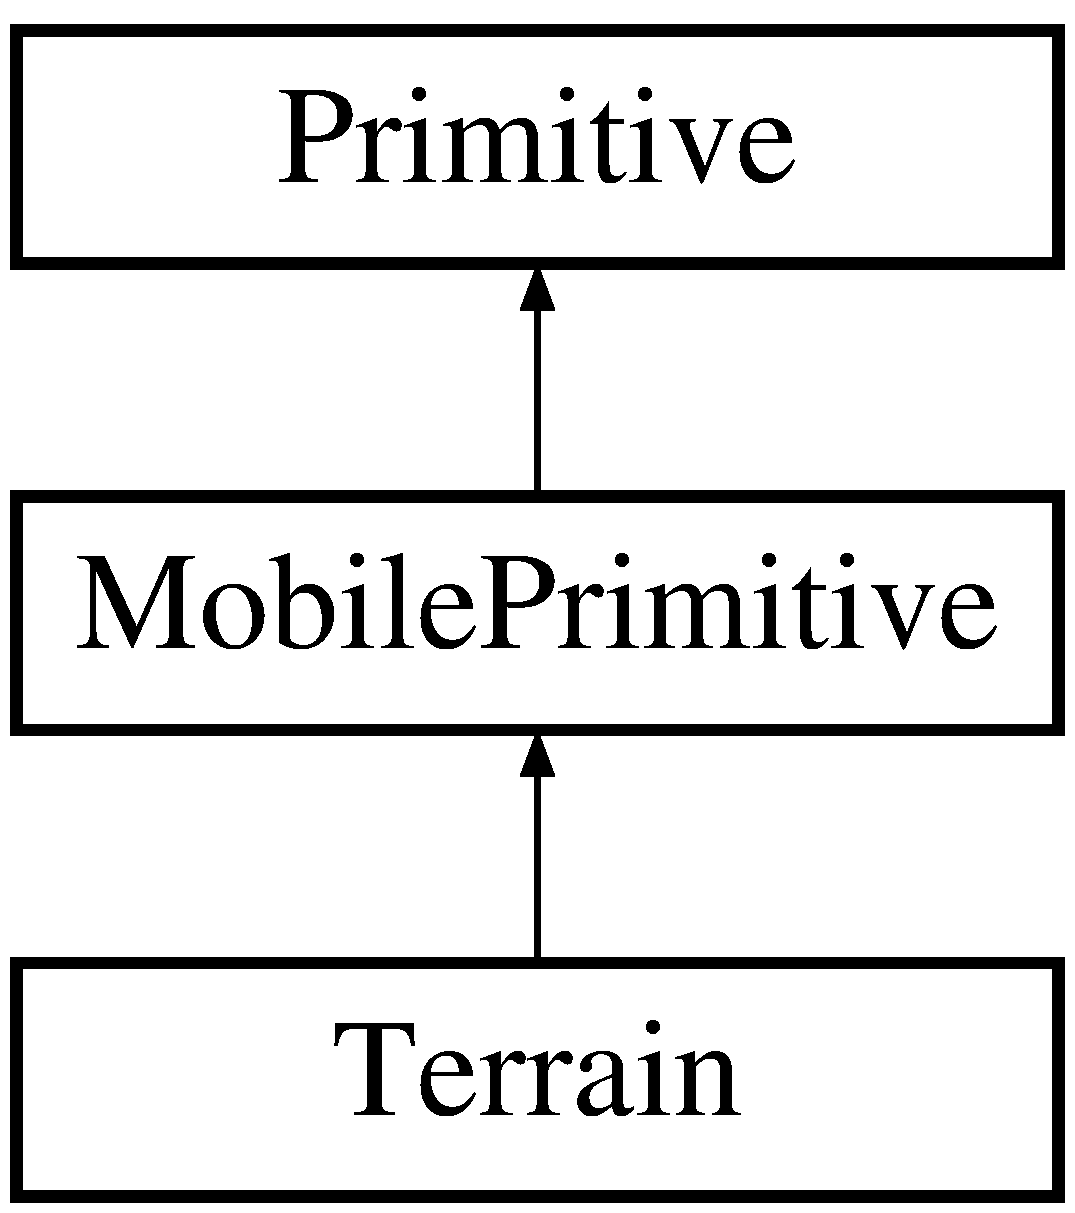
\includegraphics[height=3.000000cm]{class_mobile_primitive}
\end{center}
\end{figure}
\subsection*{Public Member Functions}
\begin{DoxyCompactItemize}
\item 
\hyperlink{class_mobile_primitive_a944bbf6ce02c59518d7ff004eac59ff1}{Mobile\-Primitive} ()
\item 
\hyperlink{class_mobile_primitive_a79b6e9202e7d3aca9d7bf4f45f61cf62}{$\sim$\-Mobile\-Primitive} ()
\item 
virtual void \hyperlink{class_mobile_primitive_afa5a61ea8a1785da95a041c5afe1fa9c}{step} (double seconds)=0
\item 
virtual void \hyperlink{class_mobile_primitive_afc11ee82cea8fda2919c01116178fe1d}{gl\-Render} () const =0
\end{DoxyCompactItemize}
\subsection*{Additional Inherited Members}


\subsection{Constructor \& Destructor Documentation}
\hypertarget{class_mobile_primitive_a944bbf6ce02c59518d7ff004eac59ff1}{\index{Mobile\-Primitive@{Mobile\-Primitive}!Mobile\-Primitive@{Mobile\-Primitive}}
\index{Mobile\-Primitive@{Mobile\-Primitive}!MobilePrimitive@{Mobile\-Primitive}}
\subsubsection[{Mobile\-Primitive}]{\setlength{\rightskip}{0pt plus 5cm}Mobile\-Primitive\-::\-Mobile\-Primitive (
\begin{DoxyParamCaption}
{}
\end{DoxyParamCaption}
)}}\label{class_mobile_primitive_a944bbf6ce02c59518d7ff004eac59ff1}
\hypertarget{class_mobile_primitive_a79b6e9202e7d3aca9d7bf4f45f61cf62}{\index{Mobile\-Primitive@{Mobile\-Primitive}!$\sim$\-Mobile\-Primitive@{$\sim$\-Mobile\-Primitive}}
\index{$\sim$\-Mobile\-Primitive@{$\sim$\-Mobile\-Primitive}!MobilePrimitive@{Mobile\-Primitive}}
\subsubsection[{$\sim$\-Mobile\-Primitive}]{\setlength{\rightskip}{0pt plus 5cm}Mobile\-Primitive\-::$\sim$\-Mobile\-Primitive (
\begin{DoxyParamCaption}
{}
\end{DoxyParamCaption}
)}}\label{class_mobile_primitive_a79b6e9202e7d3aca9d7bf4f45f61cf62}


\subsection{Member Function Documentation}
\hypertarget{class_mobile_primitive_afc11ee82cea8fda2919c01116178fe1d}{\index{Mobile\-Primitive@{Mobile\-Primitive}!gl\-Render@{gl\-Render}}
\index{gl\-Render@{gl\-Render}!MobilePrimitive@{Mobile\-Primitive}}
\subsubsection[{gl\-Render}]{\setlength{\rightskip}{0pt plus 5cm}virtual void Mobile\-Primitive\-::gl\-Render (
\begin{DoxyParamCaption}
{}
\end{DoxyParamCaption}
) const\hspace{0.3cm}{\ttfamily [pure virtual]}}}\label{class_mobile_primitive_afc11ee82cea8fda2919c01116178fe1d}


Implements \hyperlink{class_primitive_aef765029fae092f0f6dd1507e18e72e0}{Primitive}.



Implemented in \hyperlink{class_terrain_a225b584a9979c6596b90294ef29ffe47}{Terrain}.

\hypertarget{class_mobile_primitive_afa5a61ea8a1785da95a041c5afe1fa9c}{\index{Mobile\-Primitive@{Mobile\-Primitive}!step@{step}}
\index{step@{step}!MobilePrimitive@{Mobile\-Primitive}}
\subsubsection[{step}]{\setlength{\rightskip}{0pt plus 5cm}virtual void Mobile\-Primitive\-::step (
\begin{DoxyParamCaption}
\item[{double}]{seconds}
\end{DoxyParamCaption}
)\hspace{0.3cm}{\ttfamily [pure virtual]}}}\label{class_mobile_primitive_afa5a61ea8a1785da95a041c5afe1fa9c}


Implemented in \hyperlink{class_terrain_a6e3b99c889dc601aa16feb05c7376c90}{Terrain}.



The documentation for this class was generated from the following files\-:\begin{DoxyCompactItemize}
\item 
C\-:/\-Users/\-Owner/\-My Programming/\-Personal Projects/\-Video\-Games/\-Optimist Racing/src/\hyperlink{_primitive_8hpp}{Primitive.\-hpp}\item 
C\-:/\-Users/\-Owner/\-My Programming/\-Personal Projects/\-Video\-Games/\-Optimist Racing/src/\hyperlink{_primitive_8cpp}{Primitive.\-cpp}\end{DoxyCompactItemize}

\hypertarget{class_octahedron2}{\section{Octahedron2 Class Reference}
\label{class_octahedron2}\index{Octahedron2@{Octahedron2}}
}


{\ttfamily \#include $<$Primitive.\-hpp$>$}

Inheritance diagram for Octahedron2\-:\begin{figure}[H]
\begin{center}
\leavevmode
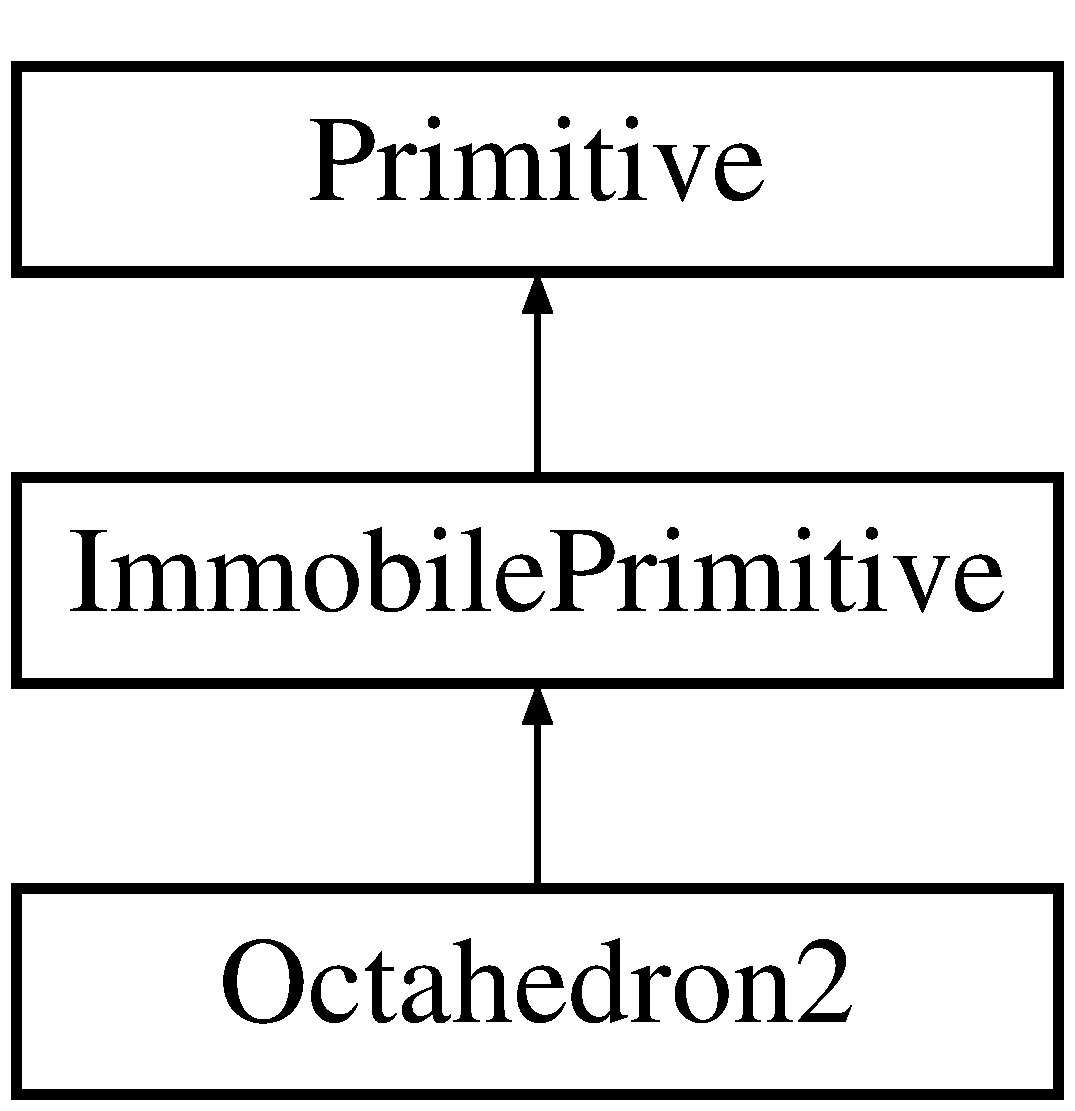
\includegraphics[height=3.000000cm]{class_octahedron2}
\end{center}
\end{figure}
\subsection*{Public Member Functions}
\begin{DoxyCompactItemize}
\item 
\hyperlink{class_octahedron2_ae61ff61ed3a6976d64ebad69122c5b17}{Octahedron2} (double radius1, double radius2, \hyperlink{class_material}{Material} $\ast$mat\-A, \hyperlink{class_material}{Material} $\ast$mat\-B, \hyperlink{class_material}{Material} $\ast$mat\-C, \hyperlink{class_material}{Material} $\ast$mat\-D, \hyperlink{class_material}{Material} $\ast$mat\-E, \hyperlink{class_material}{Material} $\ast$mat\-F, \hyperlink{class_material}{Material} $\ast$mat\-G, \hyperlink{class_material}{Material} $\ast$mat\-H)
\item 
\hyperlink{class_octahedron2_a5298f4c72c353def01fb6d35c031bbdd}{$\sim$\-Octahedron2} ()
\end{DoxyCompactItemize}
\subsection*{Additional Inherited Members}


\subsection{Constructor \& Destructor Documentation}
\hypertarget{class_octahedron2_ae61ff61ed3a6976d64ebad69122c5b17}{\index{Octahedron2@{Octahedron2}!Octahedron2@{Octahedron2}}
\index{Octahedron2@{Octahedron2}!Octahedron2@{Octahedron2}}
\subsubsection[{Octahedron2}]{\setlength{\rightskip}{0pt plus 5cm}Octahedron2\-::\-Octahedron2 (
\begin{DoxyParamCaption}
\item[{double}]{radius1, }
\item[{double}]{radius2, }
\item[{{\bf Material} $\ast$}]{mat\-A, }
\item[{{\bf Material} $\ast$}]{mat\-B, }
\item[{{\bf Material} $\ast$}]{mat\-C, }
\item[{{\bf Material} $\ast$}]{mat\-D, }
\item[{{\bf Material} $\ast$}]{mat\-E, }
\item[{{\bf Material} $\ast$}]{mat\-F, }
\item[{{\bf Material} $\ast$}]{mat\-G, }
\item[{{\bf Material} $\ast$}]{mat\-H}
\end{DoxyParamCaption}
)}}\label{class_octahedron2_ae61ff61ed3a6976d64ebad69122c5b17}
\hypertarget{class_octahedron2_a5298f4c72c353def01fb6d35c031bbdd}{\index{Octahedron2@{Octahedron2}!$\sim$\-Octahedron2@{$\sim$\-Octahedron2}}
\index{$\sim$\-Octahedron2@{$\sim$\-Octahedron2}!Octahedron2@{Octahedron2}}
\subsubsection[{$\sim$\-Octahedron2}]{\setlength{\rightskip}{0pt plus 5cm}Octahedron2\-::$\sim$\-Octahedron2 (
\begin{DoxyParamCaption}
{}
\end{DoxyParamCaption}
)}}\label{class_octahedron2_a5298f4c72c353def01fb6d35c031bbdd}


The documentation for this class was generated from the following files\-:\begin{DoxyCompactItemize}
\item 
C\-:/\-Users/\-Owner/\-My Programming/\-Personal Projects/\-Video\-Games/\-Optimist Racing/src/\hyperlink{_primitive_8hpp}{Primitive.\-hpp}\item 
C\-:/\-Users/\-Owner/\-My Programming/\-Personal Projects/\-Video\-Games/\-Optimist Racing/src/\hyperlink{_primitive_8cpp}{Primitive.\-cpp}\end{DoxyCompactItemize}

\hypertarget{class_primitive}{\section{Primitive Class Reference}
\label{class_primitive}\index{Primitive@{Primitive}}
}


{\ttfamily \#include $<$Primitive.\-hpp$>$}

Inheritance diagram for Primitive\-:\begin{figure}[H]
\begin{center}
\leavevmode
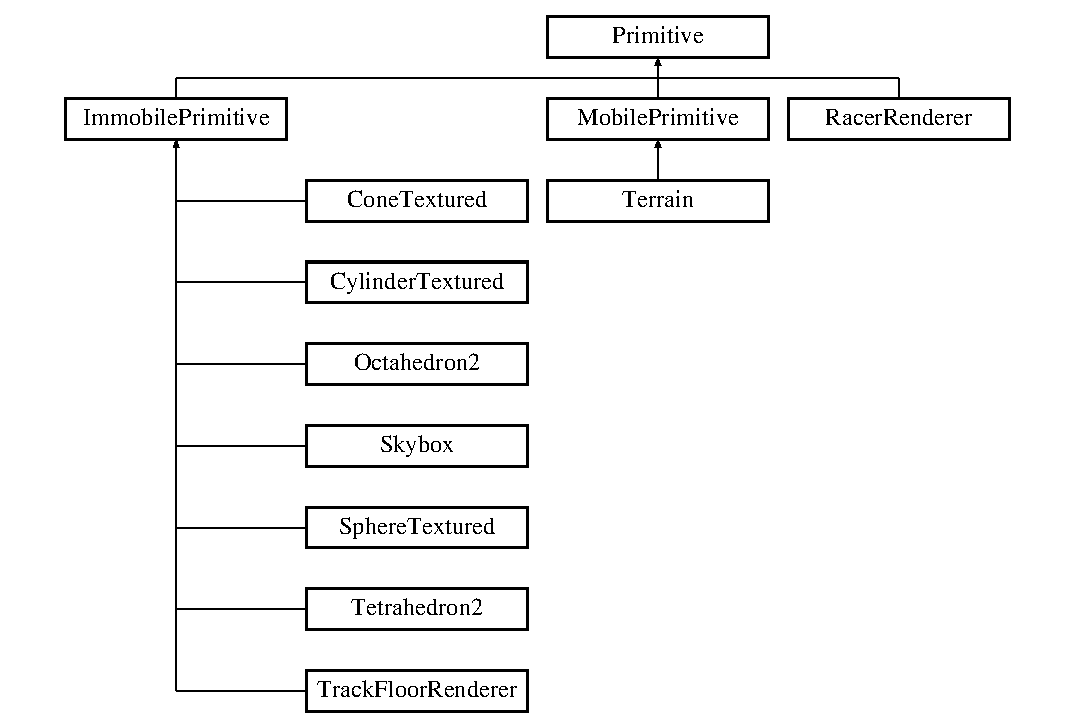
\includegraphics[height=9.000000cm]{class_primitive}
\end{center}
\end{figure}
\subsection*{Public Member Functions}
\begin{DoxyCompactItemize}
\item 
\hyperlink{class_primitive_ae6b6e9440d482575d1dcbf77a936c201}{Primitive} ()
\item 
\hyperlink{class_primitive_ad128050320901807bfe5fc20b4331db6}{$\sim$\-Primitive} ()
\item 
virtual void \hyperlink{class_primitive_aef765029fae092f0f6dd1507e18e72e0}{gl\-Render} () const =0
\end{DoxyCompactItemize}
\subsection*{Static Public Member Functions}
\begin{DoxyCompactItemize}
\item 
static void \hyperlink{class_primitive_ada024db8243a07a8adb95bceff2da718}{draw\-Triangles} (const \hyperlink{class_vector3_d}{Vector3\-D} \&center\-Vector, const \hyperlink{class_vector3_d}{Vector3\-D} $\ast$outer\-Vectors)
\item 
static void \hyperlink{class_primitive_aabe5ac74bd30711d55e78a314d3b879d}{draw\-Triangle} (const \hyperlink{class_vector3_d}{Vector3\-D} \&v1, const \hyperlink{class_vector3_d}{Vector3\-D} \&v2, const \hyperlink{class_vector3_d}{Vector3\-D} \&v3)
\item 
static void \hyperlink{class_primitive_afb79b84031c6cb7973ba61cef073e68c}{draw\-Triangle\-Pyramid} (const \hyperlink{class_vector3_d}{Vector3\-D} \&vcenter, const \hyperlink{class_vector3_d}{Vector3\-D} \&v1, const \hyperlink{class_vector3_d}{Vector3\-D} \&v2, const \hyperlink{class_vector3_d}{Vector3\-D} \&v3)
\end{DoxyCompactItemize}


\subsection{Constructor \& Destructor Documentation}
\hypertarget{class_primitive_ae6b6e9440d482575d1dcbf77a936c201}{\index{Primitive@{Primitive}!Primitive@{Primitive}}
\index{Primitive@{Primitive}!Primitive@{Primitive}}
\subsubsection[{Primitive}]{\setlength{\rightskip}{0pt plus 5cm}Primitive\-::\-Primitive (
\begin{DoxyParamCaption}
{}
\end{DoxyParamCaption}
)}}\label{class_primitive_ae6b6e9440d482575d1dcbf77a936c201}
\hypertarget{class_primitive_ad128050320901807bfe5fc20b4331db6}{\index{Primitive@{Primitive}!$\sim$\-Primitive@{$\sim$\-Primitive}}
\index{$\sim$\-Primitive@{$\sim$\-Primitive}!Primitive@{Primitive}}
\subsubsection[{$\sim$\-Primitive}]{\setlength{\rightskip}{0pt plus 5cm}Primitive\-::$\sim$\-Primitive (
\begin{DoxyParamCaption}
{}
\end{DoxyParamCaption}
)}}\label{class_primitive_ad128050320901807bfe5fc20b4331db6}


\subsection{Member Function Documentation}
\hypertarget{class_primitive_aabe5ac74bd30711d55e78a314d3b879d}{\index{Primitive@{Primitive}!draw\-Triangle@{draw\-Triangle}}
\index{draw\-Triangle@{draw\-Triangle}!Primitive@{Primitive}}
\subsubsection[{draw\-Triangle}]{\setlength{\rightskip}{0pt plus 5cm}void Primitive\-::draw\-Triangle (
\begin{DoxyParamCaption}
\item[{const {\bf Vector3\-D} \&}]{v1, }
\item[{const {\bf Vector3\-D} \&}]{v2, }
\item[{const {\bf Vector3\-D} \&}]{v3}
\end{DoxyParamCaption}
)\hspace{0.3cm}{\ttfamily [static]}}}\label{class_primitive_aabe5ac74bd30711d55e78a314d3b879d}
\hypertarget{class_primitive_afb79b84031c6cb7973ba61cef073e68c}{\index{Primitive@{Primitive}!draw\-Triangle\-Pyramid@{draw\-Triangle\-Pyramid}}
\index{draw\-Triangle\-Pyramid@{draw\-Triangle\-Pyramid}!Primitive@{Primitive}}
\subsubsection[{draw\-Triangle\-Pyramid}]{\setlength{\rightskip}{0pt plus 5cm}void Primitive\-::draw\-Triangle\-Pyramid (
\begin{DoxyParamCaption}
\item[{const {\bf Vector3\-D} \&}]{vcenter, }
\item[{const {\bf Vector3\-D} \&}]{v1, }
\item[{const {\bf Vector3\-D} \&}]{v2, }
\item[{const {\bf Vector3\-D} \&}]{v3}
\end{DoxyParamCaption}
)\hspace{0.3cm}{\ttfamily [static]}}}\label{class_primitive_afb79b84031c6cb7973ba61cef073e68c}
\hypertarget{class_primitive_ada024db8243a07a8adb95bceff2da718}{\index{Primitive@{Primitive}!draw\-Triangles@{draw\-Triangles}}
\index{draw\-Triangles@{draw\-Triangles}!Primitive@{Primitive}}
\subsubsection[{draw\-Triangles}]{\setlength{\rightskip}{0pt plus 5cm}void Primitive\-::draw\-Triangles (
\begin{DoxyParamCaption}
\item[{const {\bf Vector3\-D} \&}]{center\-Vector, }
\item[{const {\bf Vector3\-D} $\ast$}]{outer\-Vectors}
\end{DoxyParamCaption}
)\hspace{0.3cm}{\ttfamily [static]}}}\label{class_primitive_ada024db8243a07a8adb95bceff2da718}
\hypertarget{class_primitive_aef765029fae092f0f6dd1507e18e72e0}{\index{Primitive@{Primitive}!gl\-Render@{gl\-Render}}
\index{gl\-Render@{gl\-Render}!Primitive@{Primitive}}
\subsubsection[{gl\-Render}]{\setlength{\rightskip}{0pt plus 5cm}virtual void Primitive\-::gl\-Render (
\begin{DoxyParamCaption}
{}
\end{DoxyParamCaption}
) const\hspace{0.3cm}{\ttfamily [pure virtual]}}}\label{class_primitive_aef765029fae092f0f6dd1507e18e72e0}


Implemented in \hyperlink{class_racer_renderer_acd7981861dda4a5507f0771e5a3dff19}{Racer\-Renderer}, \hyperlink{class_terrain_a225b584a9979c6596b90294ef29ffe47}{Terrain}, \hyperlink{class_mobile_primitive_afc11ee82cea8fda2919c01116178fe1d}{Mobile\-Primitive}, and \hyperlink{class_immobile_primitive_ac6307f4bb055921e8727fd9a08d5dcce}{Immobile\-Primitive}.



The documentation for this class was generated from the following files\-:\begin{DoxyCompactItemize}
\item 
C\-:/\-Users/\-Owner/\-My Programming/\-Personal Projects/\-Video\-Games/\-Optimist Racing/src/\hyperlink{_primitive_8hpp}{Primitive.\-hpp}\item 
C\-:/\-Users/\-Owner/\-My Programming/\-Personal Projects/\-Video\-Games/\-Optimist Racing/src/\hyperlink{_primitive_8cpp}{Primitive.\-cpp}\end{DoxyCompactItemize}

\hypertarget{class_racer_camera}{\section{Racer\-Camera Class Reference}
\label{class_racer_camera}\index{Racer\-Camera@{Racer\-Camera}}
}


This camera will follow a racer from behind.  




{\ttfamily \#include $<$Camera.\-hpp$>$}

Inheritance diagram for Racer\-Camera\-:\begin{figure}[H]
\begin{center}
\leavevmode
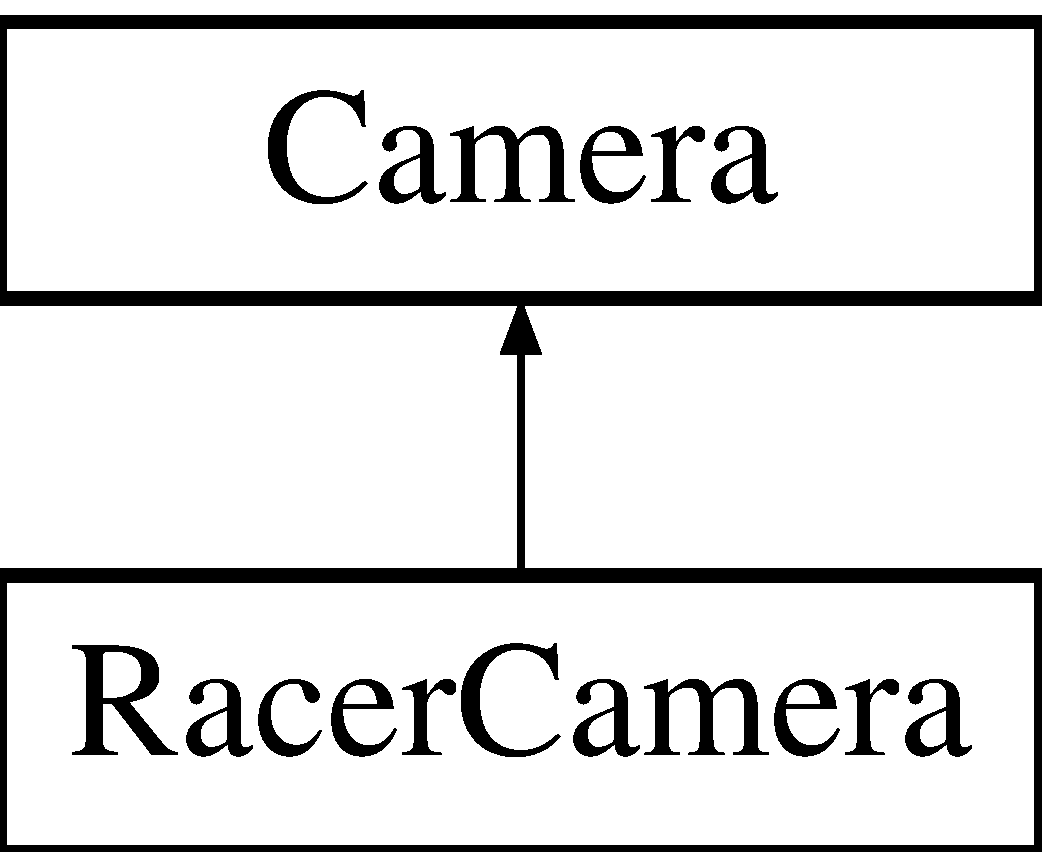
\includegraphics[height=2.000000cm]{class_racer_camera}
\end{center}
\end{figure}
\subsection*{Public Member Functions}
\begin{DoxyCompactItemize}
\item 
\hyperlink{class_racer_camera_aedc09fd0d4f894d115ec5952c3caa235}{Racer\-Camera} (\hyperlink{class_lagrange_1_1_lagrangian_racer}{Lagrangian\-Racer} $\ast$racer, double focus\-Length\-Factor, double position\-Length\-Factor, double backup\-Base, double backup\-Factor, double rotation\-Factor)
\item 
\hyperlink{class_racer_camera_a01a2fbfaf48a1044a75c5cbe924aea1b}{$\sim$\-Racer\-Camera} ()
\item 
void \hyperlink{class_racer_camera_ad062bb4bd392024505d95d225b6a1128}{set\-Lagrangian\-Racer} (\hyperlink{class_lagrange_1_1_lagrangian_racer}{Lagrangian\-Racer} $\ast$racer)
\item 
virtual void \hyperlink{class_racer_camera_a5e8a09a6290c7284cfc22ec3a8153dac}{gl\-Apply} ()
\end{DoxyCompactItemize}
\subsection*{Additional Inherited Members}


\subsection{Detailed Description}
This camera will follow a racer from behind. 

\subsection{Constructor \& Destructor Documentation}
\hypertarget{class_racer_camera_aedc09fd0d4f894d115ec5952c3caa235}{\index{Racer\-Camera@{Racer\-Camera}!Racer\-Camera@{Racer\-Camera}}
\index{Racer\-Camera@{Racer\-Camera}!RacerCamera@{Racer\-Camera}}
\subsubsection[{Racer\-Camera}]{\setlength{\rightskip}{0pt plus 5cm}Racer\-Camera\-::\-Racer\-Camera (
\begin{DoxyParamCaption}
\item[{{\bf Lagrangian\-Racer} $\ast$}]{racer, }
\item[{double}]{focus\-Length\-Factor, }
\item[{double}]{position\-Length\-Factor, }
\item[{double}]{backup\-Base, }
\item[{double}]{backup\-Factor, }
\item[{double}]{rotation\-Factor}
\end{DoxyParamCaption}
)}}\label{class_racer_camera_aedc09fd0d4f894d115ec5952c3caa235}
Sets up the camera to follow racer. \hypertarget{class_racer_camera_a01a2fbfaf48a1044a75c5cbe924aea1b}{\index{Racer\-Camera@{Racer\-Camera}!$\sim$\-Racer\-Camera@{$\sim$\-Racer\-Camera}}
\index{$\sim$\-Racer\-Camera@{$\sim$\-Racer\-Camera}!RacerCamera@{Racer\-Camera}}
\subsubsection[{$\sim$\-Racer\-Camera}]{\setlength{\rightskip}{0pt plus 5cm}Racer\-Camera\-::$\sim$\-Racer\-Camera (
\begin{DoxyParamCaption}
{}
\end{DoxyParamCaption}
)}}\label{class_racer_camera_a01a2fbfaf48a1044a75c5cbe924aea1b}
Doesn't do anything. The racer pointer is not destroyed. 

\subsection{Member Function Documentation}
\hypertarget{class_racer_camera_a5e8a09a6290c7284cfc22ec3a8153dac}{\index{Racer\-Camera@{Racer\-Camera}!gl\-Apply@{gl\-Apply}}
\index{gl\-Apply@{gl\-Apply}!RacerCamera@{Racer\-Camera}}
\subsubsection[{gl\-Apply}]{\setlength{\rightskip}{0pt plus 5cm}void Racer\-Camera\-::gl\-Apply (
\begin{DoxyParamCaption}
{}
\end{DoxyParamCaption}
)\hspace{0.3cm}{\ttfamily [virtual]}}}\label{class_racer_camera_a5e8a09a6290c7284cfc22ec3a8153dac}
Implements \hyperlink{class_camera_af3a878a62730b49ab38b33c75325342e}{Camera\-::gl\-Apply} 

Implements \hyperlink{class_camera_af3a878a62730b49ab38b33c75325342e}{Camera}.

\hypertarget{class_racer_camera_ad062bb4bd392024505d95d225b6a1128}{\index{Racer\-Camera@{Racer\-Camera}!set\-Lagrangian\-Racer@{set\-Lagrangian\-Racer}}
\index{set\-Lagrangian\-Racer@{set\-Lagrangian\-Racer}!RacerCamera@{Racer\-Camera}}
\subsubsection[{set\-Lagrangian\-Racer}]{\setlength{\rightskip}{0pt plus 5cm}void Racer\-Camera\-::set\-Lagrangian\-Racer (
\begin{DoxyParamCaption}
\item[{{\bf Lagrangian\-Racer} $\ast$}]{racer}
\end{DoxyParamCaption}
)}}\label{class_racer_camera_ad062bb4bd392024505d95d225b6a1128}
Starts following another racer. 

The documentation for this class was generated from the following files\-:\begin{DoxyCompactItemize}
\item 
C\-:/\-Users/\-Owner/\-My Programming/\-Personal Projects/\-Video\-Games/\-Optimist Racing/src/\hyperlink{_camera_8hpp}{Camera.\-hpp}\item 
C\-:/\-Users/\-Owner/\-My Programming/\-Personal Projects/\-Video\-Games/\-Optimist Racing/src/\hyperlink{_camera_8cpp}{Camera.\-cpp}\end{DoxyCompactItemize}

\hypertarget{class_racer_renderer}{\section{Racer\-Renderer Class Reference}
\label{class_racer_renderer}\index{Racer\-Renderer@{Racer\-Renderer}}
}


{\ttfamily \#include $<$Primitive.\-hpp$>$}

Inheritance diagram for Racer\-Renderer\-:\begin{figure}[H]
\begin{center}
\leavevmode
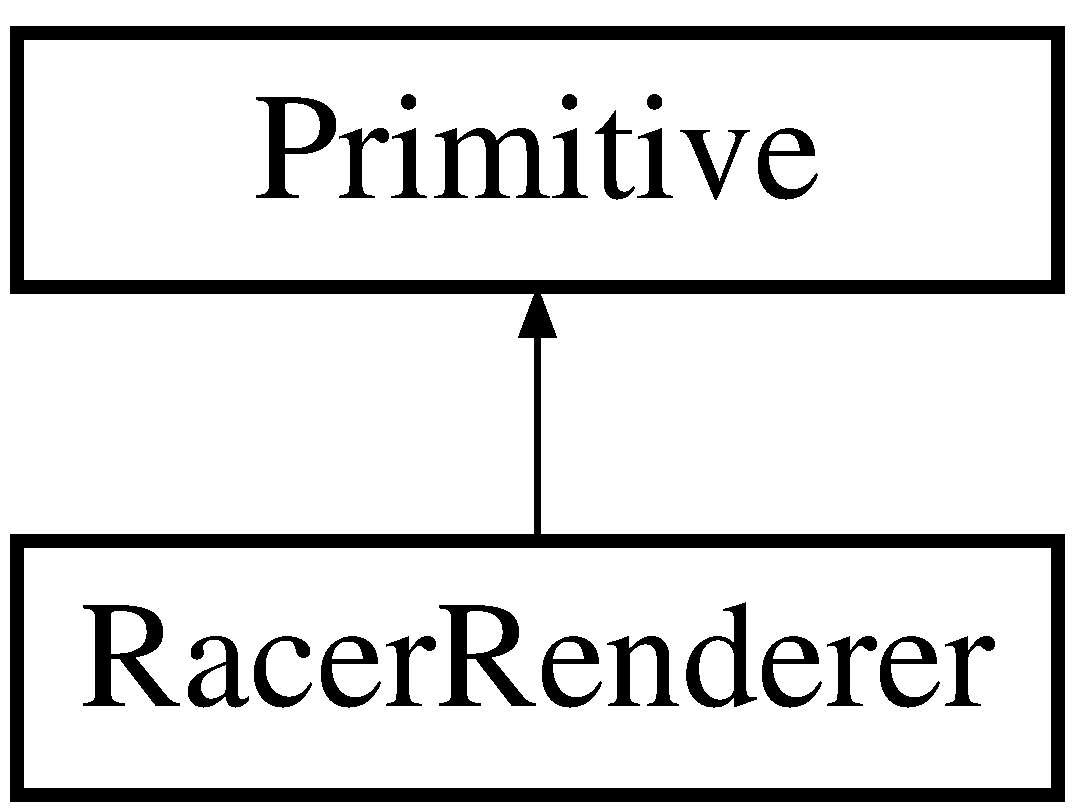
\includegraphics[height=2.000000cm]{class_racer_renderer}
\end{center}
\end{figure}
\subsection*{Public Member Functions}
\begin{DoxyCompactItemize}
\item 
\hyperlink{class_racer_renderer_a4729c12e93c352f2b4edc2bd6fcc49b8}{Racer\-Renderer} (\hyperlink{class_lagrange_1_1_lagrangian_racer}{Lagrangian\-Racer} $\ast$lagrangian\-Racer, \hyperlink{class_primitive}{Primitive} $\ast$top\-Sphere, \hyperlink{class_primitive}{Primitive} $\ast$bottom\-Sphere, \hyperlink{class_primitive}{Primitive} $\ast$cylinder, \hyperlink{class_primitive}{Primitive} $\ast$cone)
\item 
\hyperlink{class_racer_renderer_a12543cdf5d7eddd004de136b4aa2817d}{$\sim$\-Racer\-Renderer} ()
\item 
virtual void \hyperlink{class_racer_renderer_acd7981861dda4a5507f0771e5a3dff19}{gl\-Render} () const 
\end{DoxyCompactItemize}
\subsection*{Additional Inherited Members}


\subsection{Constructor \& Destructor Documentation}
\hypertarget{class_racer_renderer_a4729c12e93c352f2b4edc2bd6fcc49b8}{\index{Racer\-Renderer@{Racer\-Renderer}!Racer\-Renderer@{Racer\-Renderer}}
\index{Racer\-Renderer@{Racer\-Renderer}!RacerRenderer@{Racer\-Renderer}}
\subsubsection[{Racer\-Renderer}]{\setlength{\rightskip}{0pt plus 5cm}Racer\-Renderer\-::\-Racer\-Renderer (
\begin{DoxyParamCaption}
\item[{{\bf Lagrangian\-Racer} $\ast$}]{lagrangian\-Racer, }
\item[{{\bf Primitive} $\ast$}]{top\-Sphere, }
\item[{{\bf Primitive} $\ast$}]{bottom\-Sphere, }
\item[{{\bf Primitive} $\ast$}]{cylinder, }
\item[{{\bf Primitive} $\ast$}]{cone}
\end{DoxyParamCaption}
)}}\label{class_racer_renderer_a4729c12e93c352f2b4edc2bd6fcc49b8}
\hypertarget{class_racer_renderer_a12543cdf5d7eddd004de136b4aa2817d}{\index{Racer\-Renderer@{Racer\-Renderer}!$\sim$\-Racer\-Renderer@{$\sim$\-Racer\-Renderer}}
\index{$\sim$\-Racer\-Renderer@{$\sim$\-Racer\-Renderer}!RacerRenderer@{Racer\-Renderer}}
\subsubsection[{$\sim$\-Racer\-Renderer}]{\setlength{\rightskip}{0pt plus 5cm}Racer\-Renderer\-::$\sim$\-Racer\-Renderer (
\begin{DoxyParamCaption}
{}
\end{DoxyParamCaption}
)}}\label{class_racer_renderer_a12543cdf5d7eddd004de136b4aa2817d}


\subsection{Member Function Documentation}
\hypertarget{class_racer_renderer_acd7981861dda4a5507f0771e5a3dff19}{\index{Racer\-Renderer@{Racer\-Renderer}!gl\-Render@{gl\-Render}}
\index{gl\-Render@{gl\-Render}!RacerRenderer@{Racer\-Renderer}}
\subsubsection[{gl\-Render}]{\setlength{\rightskip}{0pt plus 5cm}void Racer\-Renderer\-::gl\-Render (
\begin{DoxyParamCaption}
{}
\end{DoxyParamCaption}
) const\hspace{0.3cm}{\ttfamily [virtual]}}}\label{class_racer_renderer_acd7981861dda4a5507f0771e5a3dff19}


Implements \hyperlink{class_primitive_aef765029fae092f0f6dd1507e18e72e0}{Primitive}.



The documentation for this class was generated from the following files\-:\begin{DoxyCompactItemize}
\item 
C\-:/\-Users/\-Owner/\-My Programming/\-Personal Projects/\-Video\-Games/\-Optimist Racing/src/\hyperlink{_primitive_8hpp}{Primitive.\-hpp}\item 
C\-:/\-Users/\-Owner/\-My Programming/\-Personal Projects/\-Video\-Games/\-Optimist Racing/src/\hyperlink{_primitive_8cpp}{Primitive.\-cpp}\end{DoxyCompactItemize}

\hypertarget{class_skybox}{\section{Skybox Class Reference}
\label{class_skybox}\index{Skybox@{Skybox}}
}


{\ttfamily \#include $<$Primitive.\-hpp$>$}

Inheritance diagram for Skybox\-:\begin{figure}[H]
\begin{center}
\leavevmode
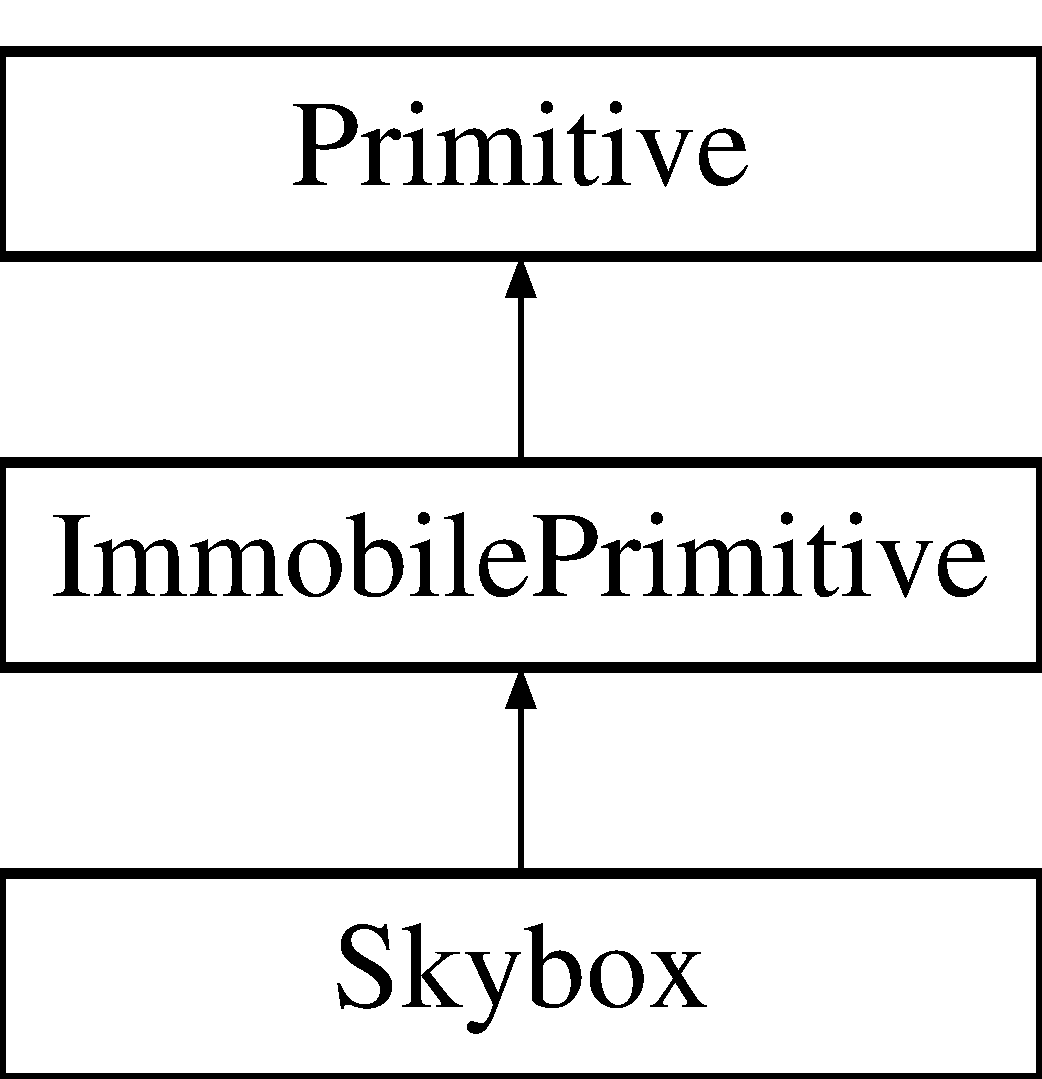
\includegraphics[height=3.000000cm]{class_skybox}
\end{center}
\end{figure}
\subsection*{Public Member Functions}
\begin{DoxyCompactItemize}
\item 
\hyperlink{class_skybox_afc61cfd31346170303119c316a2eb7f4}{Skybox} (\hyperlink{class_texture}{Texture} $\ast$texture, double halfsize, double height)
\item 
\hyperlink{class_skybox_a62ad4c6b4b1965a0a6d8536a50d4c090}{$\sim$\-Skybox} ()
\end{DoxyCompactItemize}
\subsection*{Additional Inherited Members}


\subsection{Constructor \& Destructor Documentation}
\hypertarget{class_skybox_afc61cfd31346170303119c316a2eb7f4}{\index{Skybox@{Skybox}!Skybox@{Skybox}}
\index{Skybox@{Skybox}!Skybox@{Skybox}}
\subsubsection[{Skybox}]{\setlength{\rightskip}{0pt plus 5cm}Skybox\-::\-Skybox (
\begin{DoxyParamCaption}
\item[{{\bf Texture} $\ast$}]{texture, }
\item[{double}]{halfsize, }
\item[{double}]{height}
\end{DoxyParamCaption}
)}}\label{class_skybox_afc61cfd31346170303119c316a2eb7f4}
\hypertarget{class_skybox_a62ad4c6b4b1965a0a6d8536a50d4c090}{\index{Skybox@{Skybox}!$\sim$\-Skybox@{$\sim$\-Skybox}}
\index{$\sim$\-Skybox@{$\sim$\-Skybox}!Skybox@{Skybox}}
\subsubsection[{$\sim$\-Skybox}]{\setlength{\rightskip}{0pt plus 5cm}Skybox\-::$\sim$\-Skybox (
\begin{DoxyParamCaption}
{}
\end{DoxyParamCaption}
)}}\label{class_skybox_a62ad4c6b4b1965a0a6d8536a50d4c090}


The documentation for this class was generated from the following files\-:\begin{DoxyCompactItemize}
\item 
C\-:/\-Users/\-Owner/\-My Programming/\-Personal Projects/\-Video\-Games/\-Optimist Racing/src/\hyperlink{_primitive_8hpp}{Primitive.\-hpp}\item 
C\-:/\-Users/\-Owner/\-My Programming/\-Personal Projects/\-Video\-Games/\-Optimist Racing/src/\hyperlink{_primitive_8cpp}{Primitive.\-cpp}\end{DoxyCompactItemize}

\hypertarget{class_documentation_example_1_1_some_nice_class}{\section{Documentation\-Example\-:\-:Some\-Nice\-Class Class Reference}
\label{class_documentation_example_1_1_some_nice_class}\index{Documentation\-Example\-::\-Some\-Nice\-Class@{Documentation\-Example\-::\-Some\-Nice\-Class}}
}


Pretty nice class.  




{\ttfamily \#include $<$Documentation\-Example.\-hpp$>$}

\subsection*{Public Member Functions}
\begin{DoxyCompactItemize}
\item 
\hyperlink{class_documentation_example_1_1_some_nice_class_a2eba9b893fc9eb8b4f8dfcaa76745e6e}{Some\-Nice\-Class} (double x, double y)
\begin{DoxyCompactList}\small\item\em Pretty nice constructor. \end{DoxyCompactList}\item 
\hyperlink{class_documentation_example_1_1_some_nice_class_a8f62e97b6ac0ee8d3f3f34f7d9c57c87}{$\sim$\-Some\-Nice\-Class} ()
\begin{DoxyCompactList}\small\item\em Pretty nice destructor. \end{DoxyCompactList}\item 
double \hyperlink{class_documentation_example_1_1_some_nice_class_a610a11f2c60040aa06b5fb60a6e60a48}{function1} (int a)
\begin{DoxyCompactList}\small\item\em Pretty nice function of an integer. \end{DoxyCompactList}\end{DoxyCompactItemize}


\subsection{Detailed Description}
Pretty nice class. 

This class is used to demonstrate a number of section commands. \begin{DoxyAuthor}{Author}
John Doe 

Jan Doe 
\end{DoxyAuthor}
\begin{DoxyVersion}{Version}
4.\-1a 
\end{DoxyVersion}
\begin{DoxyDate}{Date}
2012-\/2018 
\end{DoxyDate}
\begin{DoxyPrecond}{Precondition}
First initialize the system. 
\end{DoxyPrecond}
\begin{DoxyWarning}{Warning}
Improper use can crash your application 
\end{DoxyWarning}
\begin{DoxyInvariant}{Invariant}
This class's x value never changes! 
\end{DoxyInvariant}
\begin{DoxyRefDesc}{Bug}
\item[\hyperlink{bug__bug000002}{Bug}]Not all memory is freed when deleting an object of this class. \end{DoxyRefDesc}
\begin{DoxyRefDesc}{Todo}
\item[\hyperlink{todo__todo000003}{Todo}]Make the class better. \end{DoxyRefDesc}


\subsection{Constructor \& Destructor Documentation}
\hypertarget{class_documentation_example_1_1_some_nice_class_a2eba9b893fc9eb8b4f8dfcaa76745e6e}{\index{Documentation\-Example\-::\-Some\-Nice\-Class@{Documentation\-Example\-::\-Some\-Nice\-Class}!Some\-Nice\-Class@{Some\-Nice\-Class}}
\index{Some\-Nice\-Class@{Some\-Nice\-Class}!DocumentationExample::SomeNiceClass@{Documentation\-Example\-::\-Some\-Nice\-Class}}
\subsubsection[{Some\-Nice\-Class}]{\setlength{\rightskip}{0pt plus 5cm}Documentation\-Example\-::\-Some\-Nice\-Class\-::\-Some\-Nice\-Class (
\begin{DoxyParamCaption}
\item[{double}]{x, }
\item[{double}]{y}
\end{DoxyParamCaption}
)}}\label{class_documentation_example_1_1_some_nice_class_a2eba9b893fc9eb8b4f8dfcaa76745e6e}


Pretty nice constructor. 

This constructor is used to demonstrate a number of section commands. \begin{DoxyPrecond}{Precondition}
You must initialize the system first. 
\end{DoxyPrecond}
\begin{DoxyPostcond}{Postcondition}
The object will have the values x and y. 
\end{DoxyPostcond}

\begin{DoxyParams}[1]{Parameters}
\mbox{\tt in}  & {\em x} & The 1st value in the class. \\
\hline
\mbox{\tt in}  & {\em y} & The 2nd value in the class. \\
\hline
\end{DoxyParams}

\begin{DoxyExceptions}{Exceptions}
{\em An} & error when y is a prime integer. \\
\hline
\end{DoxyExceptions}
\begin{DoxyRefDesc}{Bug}
\item[\hyperlink{bug__bug000004}{Bug}]An error occurs if {\itshape y} is equal to 42,003,583. \end{DoxyRefDesc}
\begin{DoxyRefDesc}{Todo}
\item[\hyperlink{todo__todo000005}{Todo}]Make the method better by passing in another argument. \end{DoxyRefDesc}
\hypertarget{class_documentation_example_1_1_some_nice_class_a8f62e97b6ac0ee8d3f3f34f7d9c57c87}{\index{Documentation\-Example\-::\-Some\-Nice\-Class@{Documentation\-Example\-::\-Some\-Nice\-Class}!$\sim$\-Some\-Nice\-Class@{$\sim$\-Some\-Nice\-Class}}
\index{$\sim$\-Some\-Nice\-Class@{$\sim$\-Some\-Nice\-Class}!DocumentationExample::SomeNiceClass@{Documentation\-Example\-::\-Some\-Nice\-Class}}
\subsubsection[{$\sim$\-Some\-Nice\-Class}]{\setlength{\rightskip}{0pt plus 5cm}Documentation\-Example\-::\-Some\-Nice\-Class\-::$\sim$\-Some\-Nice\-Class (
\begin{DoxyParamCaption}
{}
\end{DoxyParamCaption}
)}}\label{class_documentation_example_1_1_some_nice_class_a8f62e97b6ac0ee8d3f3f34f7d9c57c87}


Pretty nice destructor. 

This constructor is used to demonstrate documentation of a destructor in a class. \begin{DoxyPrecond}{Precondition}
You must initialize the system first. 
\end{DoxyPrecond}
\begin{DoxyPostcond}{Postcondition}
The entire computer will be destroyed in a firey blaze, not just this object. 
\end{DoxyPostcond}

\begin{DoxyExceptions}{Exceptions}
{\em An} & error when something goes wrong in the destructor. \\
\hline
\end{DoxyExceptions}
\begin{DoxyRefDesc}{Bug}
\item[\hyperlink{bug__bug000005}{Bug}]The error occurs when it's not supposed to. \end{DoxyRefDesc}
\begin{DoxyRefDesc}{Todo}
\item[\hyperlink{todo__todo000006}{Todo}]Make the method better by passing in another argument. \end{DoxyRefDesc}


\subsection{Member Function Documentation}
\hypertarget{class_documentation_example_1_1_some_nice_class_a610a11f2c60040aa06b5fb60a6e60a48}{\index{Documentation\-Example\-::\-Some\-Nice\-Class@{Documentation\-Example\-::\-Some\-Nice\-Class}!function1@{function1}}
\index{function1@{function1}!DocumentationExample::SomeNiceClass@{Documentation\-Example\-::\-Some\-Nice\-Class}}
\subsubsection[{function1}]{\setlength{\rightskip}{0pt plus 5cm}double Documentation\-Example\-::\-Some\-Nice\-Class\-::function1 (
\begin{DoxyParamCaption}
\item[{int}]{a}
\end{DoxyParamCaption}
)}}\label{class_documentation_example_1_1_some_nice_class_a610a11f2c60040aa06b5fb60a6e60a48}


Pretty nice function of an integer. 

This constructor is used to demonstrate documentation of a function in a class. \begin{DoxyPrecond}{Precondition}
{\itshape a} must be positive. 
\end{DoxyPrecond}
\begin{DoxyPostcond}{Postcondition}
The object will have the value a stored in its x value for some reason. 
\end{DoxyPostcond}

\begin{DoxyParams}{Parameters}
{\em a} & The integer you want to evaluate the function of. \\
\hline
\end{DoxyParams}
\begin{DoxyReturn}{Returns}
The function of {\itshape a}. 
\end{DoxyReturn}

\begin{DoxyExceptions}{Exceptions}
{\em An} & error when a is negative. \\
\hline
\end{DoxyExceptions}
\begin{DoxyRefDesc}{Bug}
\item[\hyperlink{bug__bug000006}{Bug}]An error occurs if {\itshape a} is equal to 42,003,583. \end{DoxyRefDesc}
\begin{DoxyRefDesc}{Todo}
\item[\hyperlink{todo__todo000007}{Todo}]Make the method better by passing in another argument. \end{DoxyRefDesc}


The documentation for this class was generated from the following file\-:\begin{DoxyCompactItemize}
\item 
C\-:/\-Users/\-Owner/\-My Programming/\-Personal Projects/\-Video\-Games/\-Optimist Racing/src/\hyperlink{_documentation_example_8hpp}{Documentation\-Example.\-hpp}\end{DoxyCompactItemize}

\hypertarget{class_sphere_textured}{\section{Sphere\-Textured Class Reference}
\label{class_sphere_textured}\index{Sphere\-Textured@{Sphere\-Textured}}
}


{\ttfamily \#include $<$Primitive.\-hpp$>$}

Inheritance diagram for Sphere\-Textured\-:\begin{figure}[H]
\begin{center}
\leavevmode
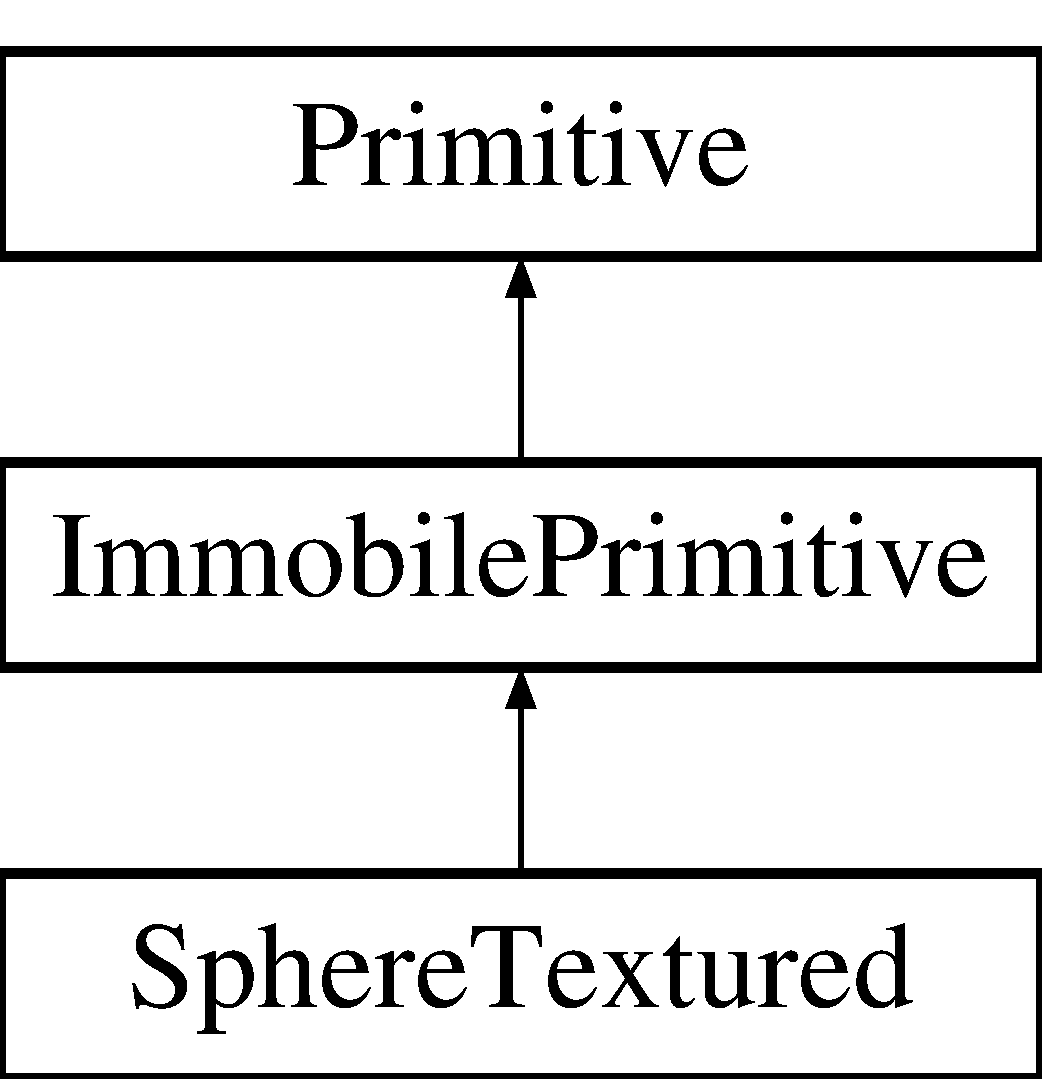
\includegraphics[height=3.000000cm]{class_sphere_textured}
\end{center}
\end{figure}
\subsection*{Public Member Functions}
\begin{DoxyCompactItemize}
\item 
\hyperlink{class_sphere_textured_a4f74ca17aac4c4e79714fad43c2baa2a}{Sphere\-Textured} (double radius, int num\-Slices, int num\-Stacks, \hyperlink{class_texture}{Texture} $\ast$texture, double num\-Textures\-X, double num\-Textures\-Y)
\item 
\hyperlink{class_sphere_textured_a5eb156e3eb2607d203067c67c26b8fe9}{$\sim$\-Sphere\-Textured} ()
\end{DoxyCompactItemize}
\subsection*{Additional Inherited Members}


\subsection{Constructor \& Destructor Documentation}
\hypertarget{class_sphere_textured_a4f74ca17aac4c4e79714fad43c2baa2a}{\index{Sphere\-Textured@{Sphere\-Textured}!Sphere\-Textured@{Sphere\-Textured}}
\index{Sphere\-Textured@{Sphere\-Textured}!SphereTextured@{Sphere\-Textured}}
\subsubsection[{Sphere\-Textured}]{\setlength{\rightskip}{0pt plus 5cm}Sphere\-Textured\-::\-Sphere\-Textured (
\begin{DoxyParamCaption}
\item[{double}]{radius, }
\item[{int}]{num\-Slices, }
\item[{int}]{num\-Stacks, }
\item[{{\bf Texture} $\ast$}]{texture, }
\item[{double}]{num\-Textures\-X, }
\item[{double}]{num\-Textures\-Y}
\end{DoxyParamCaption}
)}}\label{class_sphere_textured_a4f74ca17aac4c4e79714fad43c2baa2a}
\hypertarget{class_sphere_textured_a5eb156e3eb2607d203067c67c26b8fe9}{\index{Sphere\-Textured@{Sphere\-Textured}!$\sim$\-Sphere\-Textured@{$\sim$\-Sphere\-Textured}}
\index{$\sim$\-Sphere\-Textured@{$\sim$\-Sphere\-Textured}!SphereTextured@{Sphere\-Textured}}
\subsubsection[{$\sim$\-Sphere\-Textured}]{\setlength{\rightskip}{0pt plus 5cm}Sphere\-Textured\-::$\sim$\-Sphere\-Textured (
\begin{DoxyParamCaption}
{}
\end{DoxyParamCaption}
)}}\label{class_sphere_textured_a5eb156e3eb2607d203067c67c26b8fe9}


The documentation for this class was generated from the following files\-:\begin{DoxyCompactItemize}
\item 
C\-:/\-Users/\-Owner/\-My Programming/\-Personal Projects/\-Video\-Games/\-Optimist Racing/src/\hyperlink{_primitive_8hpp}{Primitive.\-hpp}\item 
C\-:/\-Users/\-Owner/\-My Programming/\-Personal Projects/\-Video\-Games/\-Optimist Racing/src/\hyperlink{_primitive_8cpp}{Primitive.\-cpp}\end{DoxyCompactItemize}

\hypertarget{class_system}{\section{System Class Reference}
\label{class_system}\index{System@{System}}
}


A physical system in Lagrangian Mechanics, which uses generalized coordinates.  




{\ttfamily \#include $<$System.\-hpp$>$}

Inheritance diagram for System\-:\begin{figure}[H]
\begin{center}
\leavevmode
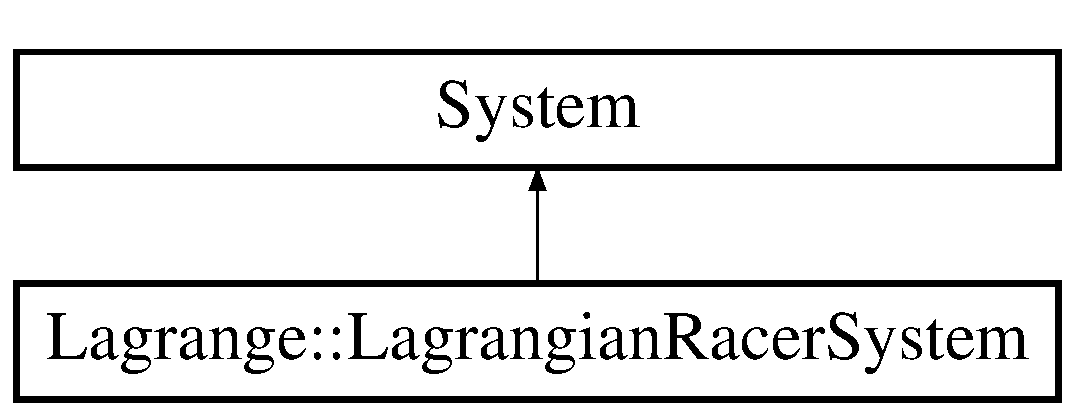
\includegraphics[height=2.000000cm]{class_system}
\end{center}
\end{figure}
\subsection*{Public Member Functions}
\begin{DoxyCompactItemize}
\item 
\hyperlink{class_system_a529efa4e15e9494ff4da5711e1d090d8}{System} (int num\-Generalized\-Coordinates)
\begin{DoxyCompactList}\small\item\em Sets the number of generalized coordinates for the system. \end{DoxyCompactList}\item 
virtual \hyperlink{struct_matrix1_vector1}{Matrix1\-Vector1} \hyperlink{class_system_adecf99535be960c23a8bb44de97cbb21}{compute\-A\-B} (const \hyperlink{class_vector_n_d}{Vector\-N\-D} \&generalized\-Position, const \hyperlink{class_vector_n_d}{Vector\-N\-D} \&generalized\-Velocity)=0
\begin{DoxyCompactList}\small\item\em Computes the matrix $A$ and the vector $\overrightarrow{b}$ such that the matrix form of the \hyperlink{namespace_lagrange}{Lagrange} equations can be written $ A \ddot{\overrightarrow{x}} + \overrightarrow{b} = \overrightarrow{Q} $. \end{DoxyCompactList}\item 
\hyperlink{class_vector_n_d}{Vector\-N\-D} \hyperlink{class_system_a785142b18417fc36453c4e72695a4f81}{compute\-Generalized\-Acceleration} (const \hyperlink{class_vector_n_d}{Vector\-N\-D} \&generalized\-Position, const \hyperlink{class_vector_n_d}{Vector\-N\-D} \&generalized\-Velocity, const \hyperlink{class_vector_n_d}{Vector\-N\-D} \&generalized\-Force)
\begin{DoxyCompactList}\small\item\em Computes the generalized acceleration as a function of the generalized position, velocity, and force. \end{DoxyCompactList}\item 
\hyperlink{class_vector_n_d}{Vector\-N\-D} \hyperlink{class_system_a61e4343973cce9211e65217379dcb1d1}{compute\-Generalized\-Acceleration} (const \hyperlink{class_vector_n_d}{Vector\-N\-D} \&generalized\-Position, const \hyperlink{class_vector_n_d}{Vector\-N\-D} \&generalized\-Velocity)
\begin{DoxyCompactList}\small\item\em Computes the generalized acceleration as a function of the generalized position and velocity. \end{DoxyCompactList}\end{DoxyCompactItemize}
\subsection*{Protected Attributes}
\begin{DoxyCompactItemize}
\item 
int \hyperlink{class_system_aa06fade2f21b3282921a86a926f0ba1f}{m\-Num\-Generalized\-Coordinates}
\begin{DoxyCompactList}\small\item\em The number of generalized coordinates in the system. \end{DoxyCompactList}\end{DoxyCompactItemize}


\subsection{Detailed Description}
A physical system in Lagrangian Mechanics, which uses generalized coordinates. 

This class handles the computation of $ \ddot{\overrightarrow{x}} $ given the generalized position vector $ \overrightarrow{x} $, the generalized velocity vector $ \dot{\overrightarrow{x}} $, and the generalized applied force vector $ \overrightarrow{Q} $. In order to use this class you need to implement the {\itshape compute\-A\-B} method, which computes the matrix $A$ and the vector $\overrightarrow{b}$ given $ \overrightarrow{x} $ and $ \dot{\overrightarrow{x}} $, such that the matrix form of the \hyperlink{namespace_lagrange}{Lagrange} equations can be written $ A \ddot{\overrightarrow{x}} + \overrightarrow{b} = \overrightarrow{Q} $. \begin{DoxyAuthor}{Author}
Claude Richard 
\end{DoxyAuthor}
\begin{DoxyVersion}{Version}
0.\-1 
\end{DoxyVersion}
\begin{DoxyDate}{Date}
2012 
\end{DoxyDate}
\begin{DoxyWarning}{Warning}
If the matrix $A$ that you compute in {\itshape compute\-A\-B} is not invertible for some values of $ \overrightarrow{x} $ and $ \dot{\overrightarrow{x}} $, then the program might crash when you call {\itshape compute\-Generalized\-Acceleration}. It is best to make sure that $A$ is invertible for all possible generalized position. 
\end{DoxyWarning}
\begin{DoxyInvariant}{Invariant}
The number of generalized coordinates $n$ in the system never changes. 
\end{DoxyInvariant}

\begin{DoxyExceptions}{Exceptions}
{\em Whenever} & you pass a vector of generalized position or velocity, it needs to have length $n$, otherwise this will throw an error. \\
\hline
\end{DoxyExceptions}
\begin{DoxyRefDesc}{Todo}
\item[\hyperlink{todo__todo000009}{Todo}]Write and implement this class. \end{DoxyRefDesc}


\subsection{Constructor \& Destructor Documentation}
\hypertarget{class_system_a529efa4e15e9494ff4da5711e1d090d8}{\index{System@{System}!System@{System}}
\index{System@{System}!System@{System}}
\subsubsection[{System}]{\setlength{\rightskip}{0pt plus 5cm}System\-::\-System (
\begin{DoxyParamCaption}
\item[{int}]{num\-Generalized\-Coordinates}
\end{DoxyParamCaption}
)}}\label{class_system_a529efa4e15e9494ff4da5711e1d090d8}


Sets the number of generalized coordinates for the system. 

This class's only piece of data stored is the number of generalized coordinates. \begin{DoxyPostcond}{Postcondition}
The object will have the number of generalized coordinates set. 
\end{DoxyPostcond}

\begin{DoxyParams}[1]{Parameters}
\mbox{\tt in}  & {\em num\-Generalized\-Coordinates} & The number of generalized coordinates. \\
\hline
\end{DoxyParams}

\begin{DoxyExceptions}{Exceptions}
{\em An} & error when {\itshape num\-Generalized\-Coordinates} $<$= 0. \\
\hline
\end{DoxyExceptions}


\subsection{Member Function Documentation}
\hypertarget{class_system_adecf99535be960c23a8bb44de97cbb21}{\index{System@{System}!compute\-A\-B@{compute\-A\-B}}
\index{compute\-A\-B@{compute\-A\-B}!System@{System}}
\subsubsection[{compute\-A\-B}]{\setlength{\rightskip}{0pt plus 5cm}virtual {\bf Matrix1\-Vector1} System\-::compute\-A\-B (
\begin{DoxyParamCaption}
\item[{const {\bf Vector\-N\-D} \&}]{generalized\-Position, }
\item[{const {\bf Vector\-N\-D} \&}]{generalized\-Velocity}
\end{DoxyParamCaption}
)\hspace{0.3cm}{\ttfamily [pure virtual]}}}\label{class_system_adecf99535be960c23a8bb44de97cbb21}


Computes the matrix $A$ and the vector $\overrightarrow{b}$ such that the matrix form of the \hyperlink{namespace_lagrange}{Lagrange} equations can be written $ A \ddot{\overrightarrow{x}} + \overrightarrow{b} = \overrightarrow{Q} $. 

This function is used in the {\itshape get\-Generalized\-Acceleration} method. \begin{DoxyPrecond}{Precondition}
Both arguments must have length equal to $n$, the number of generalized coordinates. 
\end{DoxyPrecond}

\begin{DoxyParams}{Parameters}
{\em generalized\-Position} & The generalized position vector. \\
\hline
{\em generalized\-Velocity} & The generalized velocity vector. \\
\hline
\end{DoxyParams}
\begin{DoxyReturn}{Returns}
A struct containing $A(\overrightarrow{x},\dot{\overrightarrow{x}})$ and $\overrightarrow{b}(\overrightarrow{x},\dot{\overrightarrow{x}})$ such that the matrix form of the \hyperlink{namespace_lagrange}{Lagrange} equations can be written $ A \ddot{\overrightarrow{x}} + \overrightarrow{b} = \overrightarrow{Q} $, where $\overrightarrow{Q}$ is the generalized applied force on the system. 
\end{DoxyReturn}

\begin{DoxyExceptions}{Exceptions}
{\em An} & error if the length of either generalized\-Position or generalized\-Velocity is not equal to $n$, the number of generalized coordinates. \\
\hline
\end{DoxyExceptions}
\hypertarget{class_system_a785142b18417fc36453c4e72695a4f81}{\index{System@{System}!compute\-Generalized\-Acceleration@{compute\-Generalized\-Acceleration}}
\index{compute\-Generalized\-Acceleration@{compute\-Generalized\-Acceleration}!System@{System}}
\subsubsection[{compute\-Generalized\-Acceleration}]{\setlength{\rightskip}{0pt plus 5cm}{\bf Vector\-N\-D} System\-::compute\-Generalized\-Acceleration (
\begin{DoxyParamCaption}
\item[{const {\bf Vector\-N\-D} \&}]{generalized\-Position, }
\item[{const {\bf Vector\-N\-D} \&}]{generalized\-Velocity, }
\item[{const {\bf Vector\-N\-D} \&}]{generalized\-Force}
\end{DoxyParamCaption}
)}}\label{class_system_a785142b18417fc36453c4e72695a4f81}


Computes the generalized acceleration as a function of the generalized position, velocity, and force. 

\begin{DoxyPrecond}{Precondition}
All parameters must have length $n$, the number of generalized coordinates. 
\end{DoxyPrecond}

\begin{DoxyParams}{Parameters}
{\em generalized\-Position} & The generalized position vector. \\
\hline
{\em generalized\-Velocity} & The generalized velocity vector. \\
\hline
{\em generalized\-Force} & The generalized force vector. \\
\hline
\end{DoxyParams}
\begin{DoxyReturn}{Returns}
The generalized acceleration when the position, velocity, and force are equal to the arguments. 
\end{DoxyReturn}

\begin{DoxyExceptions}{Exceptions}
{\em An} & error when either of the arguments does not have length $n$, the number of generalized coordinates. \\
\hline
\end{DoxyExceptions}
\begin{DoxyRefDesc}{Todo}
\item[\hyperlink{todo__todo000010}{Todo}]Implement this method. \end{DoxyRefDesc}
\hypertarget{class_system_a61e4343973cce9211e65217379dcb1d1}{\index{System@{System}!compute\-Generalized\-Acceleration@{compute\-Generalized\-Acceleration}}
\index{compute\-Generalized\-Acceleration@{compute\-Generalized\-Acceleration}!System@{System}}
\subsubsection[{compute\-Generalized\-Acceleration}]{\setlength{\rightskip}{0pt plus 5cm}{\bf Vector\-N\-D} System\-::compute\-Generalized\-Acceleration (
\begin{DoxyParamCaption}
\item[{const {\bf Vector\-N\-D} \&}]{generalized\-Position, }
\item[{const {\bf Vector\-N\-D} \&}]{generalized\-Velocity}
\end{DoxyParamCaption}
)}}\label{class_system_a61e4343973cce9211e65217379dcb1d1}


Computes the generalized acceleration as a function of the generalized position and velocity. 

The applied force is assumed to be zero. \begin{DoxyPrecond}{Precondition}
All parameters must have length $n$, the number of generalized coordinates. 
\end{DoxyPrecond}

\begin{DoxyParams}{Parameters}
{\em generalized\-Position} & The generalized position vector. \\
\hline
{\em generalized\-Velocity} & The generalized velocity vector. \\
\hline
\end{DoxyParams}
\begin{DoxyReturn}{Returns}
The generalized acceleration when the position and velocity are equal to the arguments and the force is zero. 
\end{DoxyReturn}

\begin{DoxyExceptions}{Exceptions}
{\em An} & error when either of the arguments does not have length $n$, the number of generalized coordinates. \\
\hline
\end{DoxyExceptions}
\begin{DoxyRefDesc}{Todo}
\item[\hyperlink{todo__todo000011}{Todo}]Implement this method. \end{DoxyRefDesc}


\subsection{Member Data Documentation}
\hypertarget{class_system_aa06fade2f21b3282921a86a926f0ba1f}{\index{System@{System}!m\-Num\-Generalized\-Coordinates@{m\-Num\-Generalized\-Coordinates}}
\index{m\-Num\-Generalized\-Coordinates@{m\-Num\-Generalized\-Coordinates}!System@{System}}
\subsubsection[{m\-Num\-Generalized\-Coordinates}]{\setlength{\rightskip}{0pt plus 5cm}int System\-::m\-Num\-Generalized\-Coordinates\hspace{0.3cm}{\ttfamily [protected]}}}\label{class_system_aa06fade2f21b3282921a86a926f0ba1f}


The number of generalized coordinates in the system. 



The documentation for this class was generated from the following files\-:\begin{DoxyCompactItemize}
\item 
C\-:/\-Users/\-Owner/\-My Programming/\-Personal Projects/\-Video\-Games/\-Optimist Racing/src/\hyperlink{_system_8hpp}{System.\-hpp}\item 
C\-:/\-Users/\-Owner/\-My Programming/\-Personal Projects/\-Video\-Games/\-Optimist Racing/src/\hyperlink{_system_8cpp}{System.\-cpp}\end{DoxyCompactItemize}

\hypertarget{class_terrain}{\section{Terrain Class Reference}
\label{class_terrain}\index{Terrain@{Terrain}}
}


{\ttfamily \#include $<$Primitive.\-hpp$>$}

Inheritance diagram for Terrain\-:\begin{figure}[H]
\begin{center}
\leavevmode
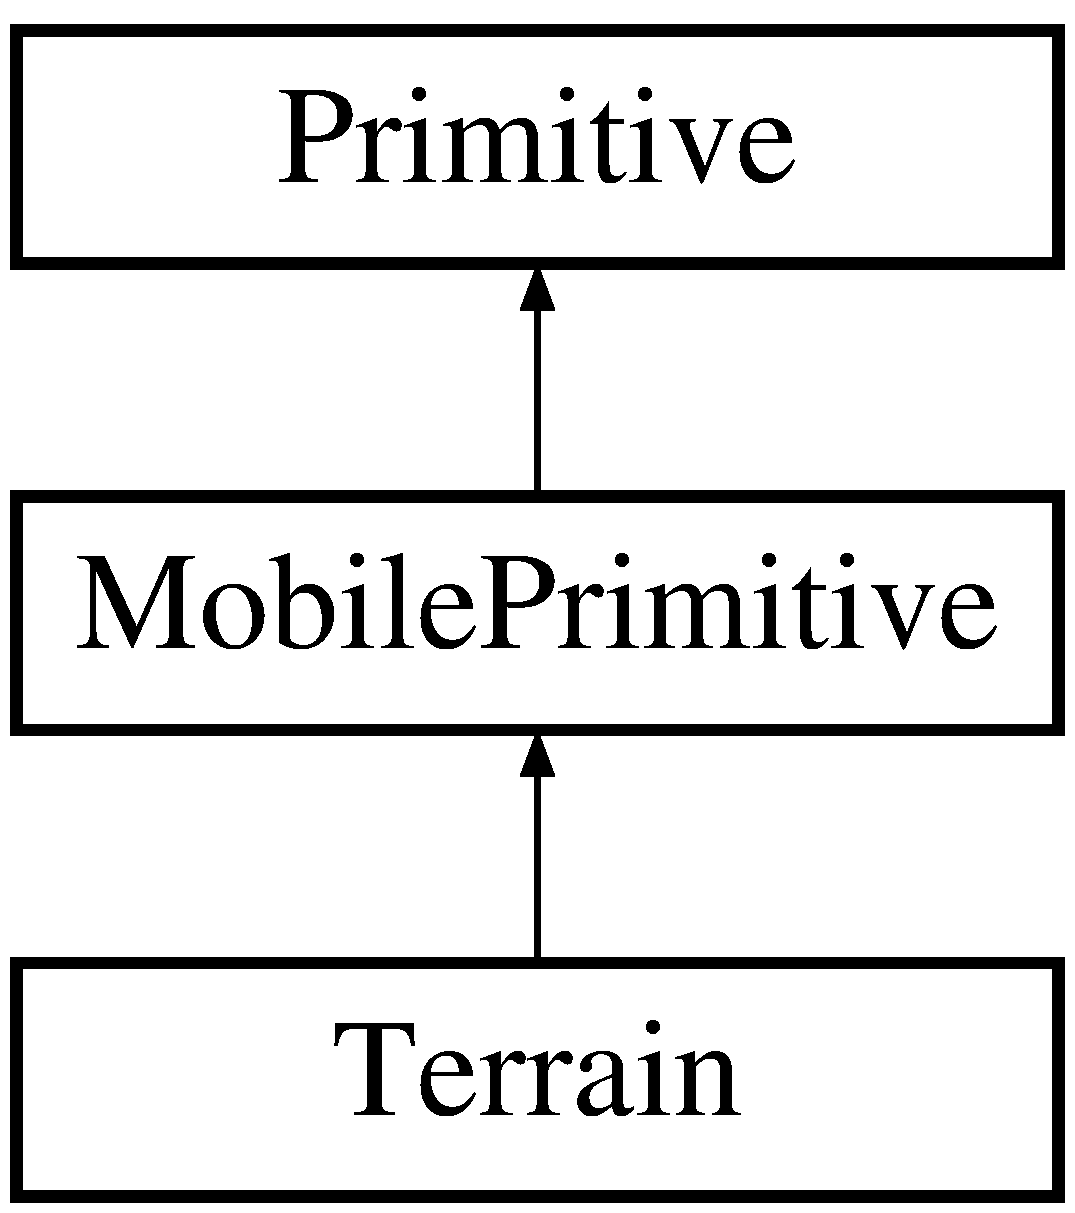
\includegraphics[height=3.000000cm]{class_terrain}
\end{center}
\end{figure}
\subsection*{Public Member Functions}
\begin{DoxyCompactItemize}
\item 
\hyperlink{class_terrain_ac3699a5130564b98316c80f5586a4467}{Terrain} (\hyperlink{class_texture}{Texture} $\ast$texture, double halfsize, double depth, double meters\-Per\-Image\-X, double meters\-Per\-Image\-Y, double speed\-X, double speed\-Y)
\item 
\hyperlink{class_terrain_a2f7f0a2aee54886324ccf48a6f321de0}{$\sim$\-Terrain} ()
\item 
virtual void \hyperlink{class_terrain_a6e3b99c889dc601aa16feb05c7376c90}{step} (double seconds)
\item 
virtual void \hyperlink{class_terrain_a225b584a9979c6596b90294ef29ffe47}{gl\-Render} () const 
\end{DoxyCompactItemize}
\subsection*{Additional Inherited Members}


\subsection{Constructor \& Destructor Documentation}
\hypertarget{class_terrain_ac3699a5130564b98316c80f5586a4467}{\index{Terrain@{Terrain}!Terrain@{Terrain}}
\index{Terrain@{Terrain}!Terrain@{Terrain}}
\subsubsection[{Terrain}]{\setlength{\rightskip}{0pt plus 5cm}Terrain\-::\-Terrain (
\begin{DoxyParamCaption}
\item[{{\bf Texture} $\ast$}]{texture, }
\item[{double}]{halfsize, }
\item[{double}]{depth, }
\item[{double}]{meters\-Per\-Image\-X, }
\item[{double}]{meters\-Per\-Image\-Y, }
\item[{double}]{speed\-X, }
\item[{double}]{speed\-Y}
\end{DoxyParamCaption}
)}}\label{class_terrain_ac3699a5130564b98316c80f5586a4467}
\hypertarget{class_terrain_a2f7f0a2aee54886324ccf48a6f321de0}{\index{Terrain@{Terrain}!$\sim$\-Terrain@{$\sim$\-Terrain}}
\index{$\sim$\-Terrain@{$\sim$\-Terrain}!Terrain@{Terrain}}
\subsubsection[{$\sim$\-Terrain}]{\setlength{\rightskip}{0pt plus 5cm}Terrain\-::$\sim$\-Terrain (
\begin{DoxyParamCaption}
{}
\end{DoxyParamCaption}
)}}\label{class_terrain_a2f7f0a2aee54886324ccf48a6f321de0}


\subsection{Member Function Documentation}
\hypertarget{class_terrain_a225b584a9979c6596b90294ef29ffe47}{\index{Terrain@{Terrain}!gl\-Render@{gl\-Render}}
\index{gl\-Render@{gl\-Render}!Terrain@{Terrain}}
\subsubsection[{gl\-Render}]{\setlength{\rightskip}{0pt plus 5cm}void Terrain\-::gl\-Render (
\begin{DoxyParamCaption}
{}
\end{DoxyParamCaption}
) const\hspace{0.3cm}{\ttfamily [virtual]}}}\label{class_terrain_a225b584a9979c6596b90294ef29ffe47}


Implements \hyperlink{class_mobile_primitive_afc11ee82cea8fda2919c01116178fe1d}{Mobile\-Primitive}.

\hypertarget{class_terrain_a6e3b99c889dc601aa16feb05c7376c90}{\index{Terrain@{Terrain}!step@{step}}
\index{step@{step}!Terrain@{Terrain}}
\subsubsection[{step}]{\setlength{\rightskip}{0pt plus 5cm}void Terrain\-::step (
\begin{DoxyParamCaption}
\item[{double}]{seconds}
\end{DoxyParamCaption}
)\hspace{0.3cm}{\ttfamily [virtual]}}}\label{class_terrain_a6e3b99c889dc601aa16feb05c7376c90}


Implements \hyperlink{class_mobile_primitive_afa5a61ea8a1785da95a041c5afe1fa9c}{Mobile\-Primitive}.



The documentation for this class was generated from the following files\-:\begin{DoxyCompactItemize}
\item 
C\-:/\-Users/\-Owner/\-My Programming/\-Personal Projects/\-Video\-Games/\-Optimist Racing/src/\hyperlink{_primitive_8hpp}{Primitive.\-hpp}\item 
C\-:/\-Users/\-Owner/\-My Programming/\-Personal Projects/\-Video\-Games/\-Optimist Racing/src/\hyperlink{_primitive_8cpp}{Primitive.\-cpp}\end{DoxyCompactItemize}

\hypertarget{class_tetrahedron2}{\section{Tetrahedron2 Class Reference}
\label{class_tetrahedron2}\index{Tetrahedron2@{Tetrahedron2}}
}


{\ttfamily \#include $<$Primitive.\-hpp$>$}

Inheritance diagram for Tetrahedron2\-:\begin{figure}[H]
\begin{center}
\leavevmode
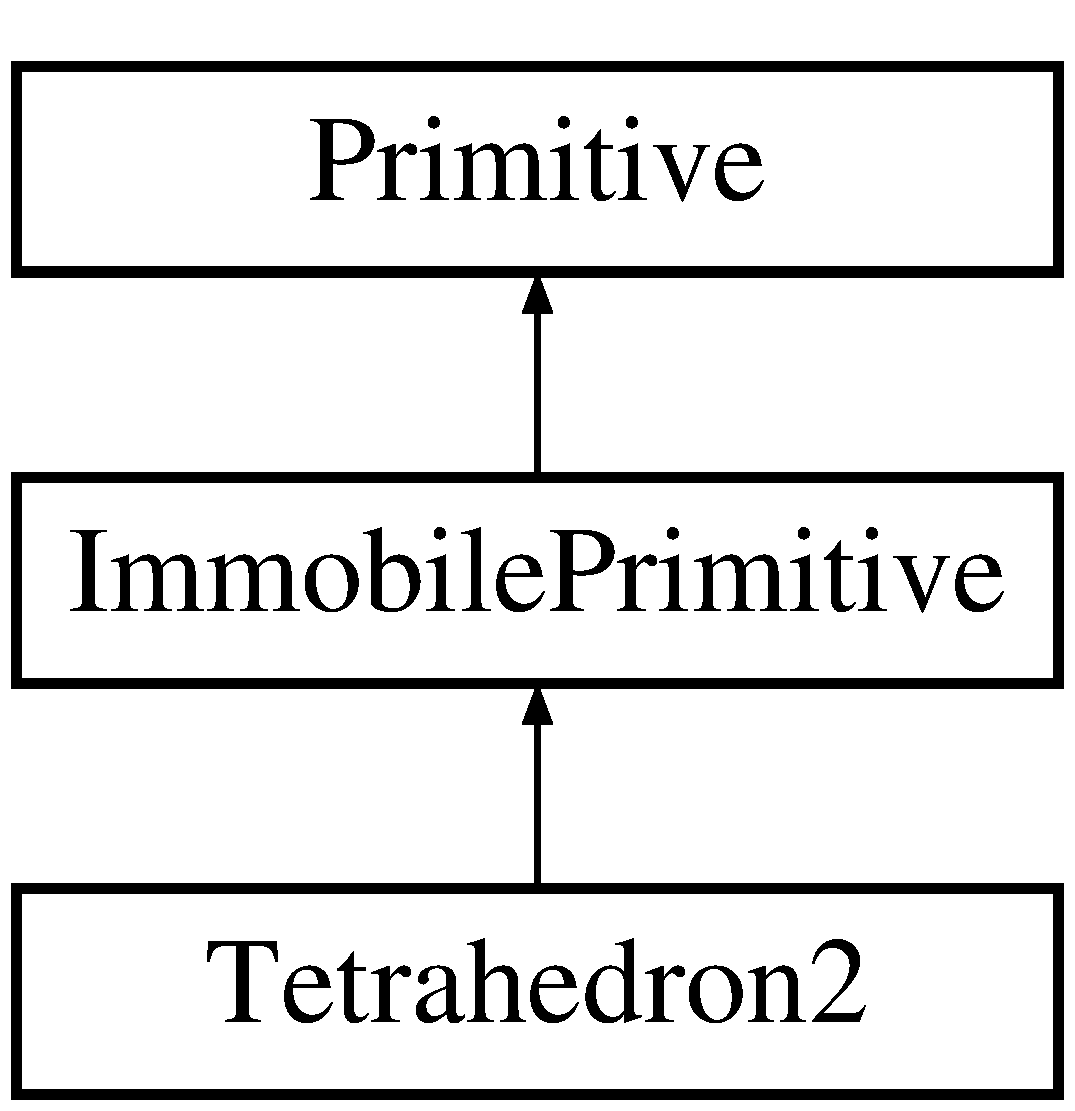
\includegraphics[height=3.000000cm]{class_tetrahedron2}
\end{center}
\end{figure}
\subsection*{Public Member Functions}
\begin{DoxyCompactItemize}
\item 
\hyperlink{class_tetrahedron2_a765d55000c92cfe28af7e7a04cf2d4cc}{Tetrahedron2} (double radius1, double radius2, \hyperlink{class_material}{Material} $\ast$mat\-Bottom, \hyperlink{class_material}{Material} $\ast$mat\-Front, \hyperlink{class_material}{Material} $\ast$mat\-Backright, \hyperlink{class_material}{Material} $\ast$mat\-Backleft)
\item 
\hyperlink{class_tetrahedron2_a668ee8aec30331661ab295df9e8b1365}{$\sim$\-Tetrahedron2} ()
\end{DoxyCompactItemize}
\subsection*{Additional Inherited Members}


\subsection{Constructor \& Destructor Documentation}
\hypertarget{class_tetrahedron2_a765d55000c92cfe28af7e7a04cf2d4cc}{\index{Tetrahedron2@{Tetrahedron2}!Tetrahedron2@{Tetrahedron2}}
\index{Tetrahedron2@{Tetrahedron2}!Tetrahedron2@{Tetrahedron2}}
\subsubsection[{Tetrahedron2}]{\setlength{\rightskip}{0pt plus 5cm}Tetrahedron2\-::\-Tetrahedron2 (
\begin{DoxyParamCaption}
\item[{double}]{radius1, }
\item[{double}]{radius2, }
\item[{{\bf Material} $\ast$}]{mat\-Bottom, }
\item[{{\bf Material} $\ast$}]{mat\-Front, }
\item[{{\bf Material} $\ast$}]{mat\-Backright, }
\item[{{\bf Material} $\ast$}]{mat\-Backleft}
\end{DoxyParamCaption}
)}}\label{class_tetrahedron2_a765d55000c92cfe28af7e7a04cf2d4cc}
\hypertarget{class_tetrahedron2_a668ee8aec30331661ab295df9e8b1365}{\index{Tetrahedron2@{Tetrahedron2}!$\sim$\-Tetrahedron2@{$\sim$\-Tetrahedron2}}
\index{$\sim$\-Tetrahedron2@{$\sim$\-Tetrahedron2}!Tetrahedron2@{Tetrahedron2}}
\subsubsection[{$\sim$\-Tetrahedron2}]{\setlength{\rightskip}{0pt plus 5cm}Tetrahedron2\-::$\sim$\-Tetrahedron2 (
\begin{DoxyParamCaption}
{}
\end{DoxyParamCaption}
)}}\label{class_tetrahedron2_a668ee8aec30331661ab295df9e8b1365}


The documentation for this class was generated from the following files\-:\begin{DoxyCompactItemize}
\item 
C\-:/\-Users/\-Owner/\-My Programming/\-Personal Projects/\-Video\-Games/\-Optimist Racing/src/\hyperlink{_primitive_8hpp}{Primitive.\-hpp}\item 
C\-:/\-Users/\-Owner/\-My Programming/\-Personal Projects/\-Video\-Games/\-Optimist Racing/src/\hyperlink{_primitive_8cpp}{Primitive.\-cpp}\end{DoxyCompactItemize}

\hypertarget{class_texture}{\section{Texture Class Reference}
\label{class_texture}\index{Texture@{Texture}}
}


{\ttfamily \#include $<$Material.\-hpp$>$}

\subsection*{Public Member Functions}
\begin{DoxyCompactItemize}
\item 
\hyperlink{class_texture_a1ec6faf3bd4d7ff15a5b7fb5c4a2439f}{Texture} (\hyperlink{class_image}{Image} $\ast$image, bool wrap)
\item 
\hyperlink{class_texture_a09c4bcb7462f64c1d20fa69dba3cee8a}{$\sim$\-Texture} ()
\item 
G\-Luint \hyperlink{class_texture_a2b1aaa87408b1447b76dc8eab3f9ff95}{gl\-Get} () const 
\item 
void \hyperlink{class_texture_a0789ca540c4d5e08a009b89e7037526d}{gl\-Apply} () const 
\end{DoxyCompactItemize}


\subsection{Detailed Description}
A \hyperlink{class_texture}{Texture} basically stores an image, which is usually read from an image file (e.\-g. P\-N\-G) so it can do texture mapping in Open\-G\-L. 

\subsection{Constructor \& Destructor Documentation}
\hypertarget{class_texture_a1ec6faf3bd4d7ff15a5b7fb5c4a2439f}{\index{Texture@{Texture}!Texture@{Texture}}
\index{Texture@{Texture}!Texture@{Texture}}
\subsubsection[{Texture}]{\setlength{\rightskip}{0pt plus 5cm}Texture\-::\-Texture (
\begin{DoxyParamCaption}
\item[{{\bf Image} $\ast$}]{image, }
\item[{bool}]{wrap}
\end{DoxyParamCaption}
)}}\label{class_texture_a1ec6faf3bd4d7ff15a5b7fb5c4a2439f}
\hypertarget{class_texture_a09c4bcb7462f64c1d20fa69dba3cee8a}{\index{Texture@{Texture}!$\sim$\-Texture@{$\sim$\-Texture}}
\index{$\sim$\-Texture@{$\sim$\-Texture}!Texture@{Texture}}
\subsubsection[{$\sim$\-Texture}]{\setlength{\rightskip}{0pt plus 5cm}Texture\-::$\sim$\-Texture (
\begin{DoxyParamCaption}
{}
\end{DoxyParamCaption}
)}}\label{class_texture_a09c4bcb7462f64c1d20fa69dba3cee8a}


\subsection{Member Function Documentation}
\hypertarget{class_texture_a0789ca540c4d5e08a009b89e7037526d}{\index{Texture@{Texture}!gl\-Apply@{gl\-Apply}}
\index{gl\-Apply@{gl\-Apply}!Texture@{Texture}}
\subsubsection[{gl\-Apply}]{\setlength{\rightskip}{0pt plus 5cm}void Texture\-::gl\-Apply (
\begin{DoxyParamCaption}
{}
\end{DoxyParamCaption}
) const}}\label{class_texture_a0789ca540c4d5e08a009b89e7037526d}
\hypertarget{class_texture_a2b1aaa87408b1447b76dc8eab3f9ff95}{\index{Texture@{Texture}!gl\-Get@{gl\-Get}}
\index{gl\-Get@{gl\-Get}!Texture@{Texture}}
\subsubsection[{gl\-Get}]{\setlength{\rightskip}{0pt plus 5cm}G\-Luint Texture\-::gl\-Get (
\begin{DoxyParamCaption}
{}
\end{DoxyParamCaption}
) const}}\label{class_texture_a2b1aaa87408b1447b76dc8eab3f9ff95}


The documentation for this class was generated from the following files\-:\begin{DoxyCompactItemize}
\item 
C\-:/\-Users/\-Owner/\-My Programming/\-Personal Projects/\-Video\-Games/\-Optimist Racing/src/\hyperlink{_material_8hpp}{Material.\-hpp}\item 
C\-:/\-Users/\-Owner/\-My Programming/\-Personal Projects/\-Video\-Games/\-Optimist Racing/src/\hyperlink{_material_8cpp}{Material.\-cpp}\end{DoxyCompactItemize}

\hypertarget{class_track_floor_renderer}{\section{Track\-Floor\-Renderer Class Reference}
\label{class_track_floor_renderer}\index{Track\-Floor\-Renderer@{Track\-Floor\-Renderer}}
}


{\ttfamily \#include $<$Primitive.\-hpp$>$}

Inheritance diagram for Track\-Floor\-Renderer\-:\begin{figure}[H]
\begin{center}
\leavevmode
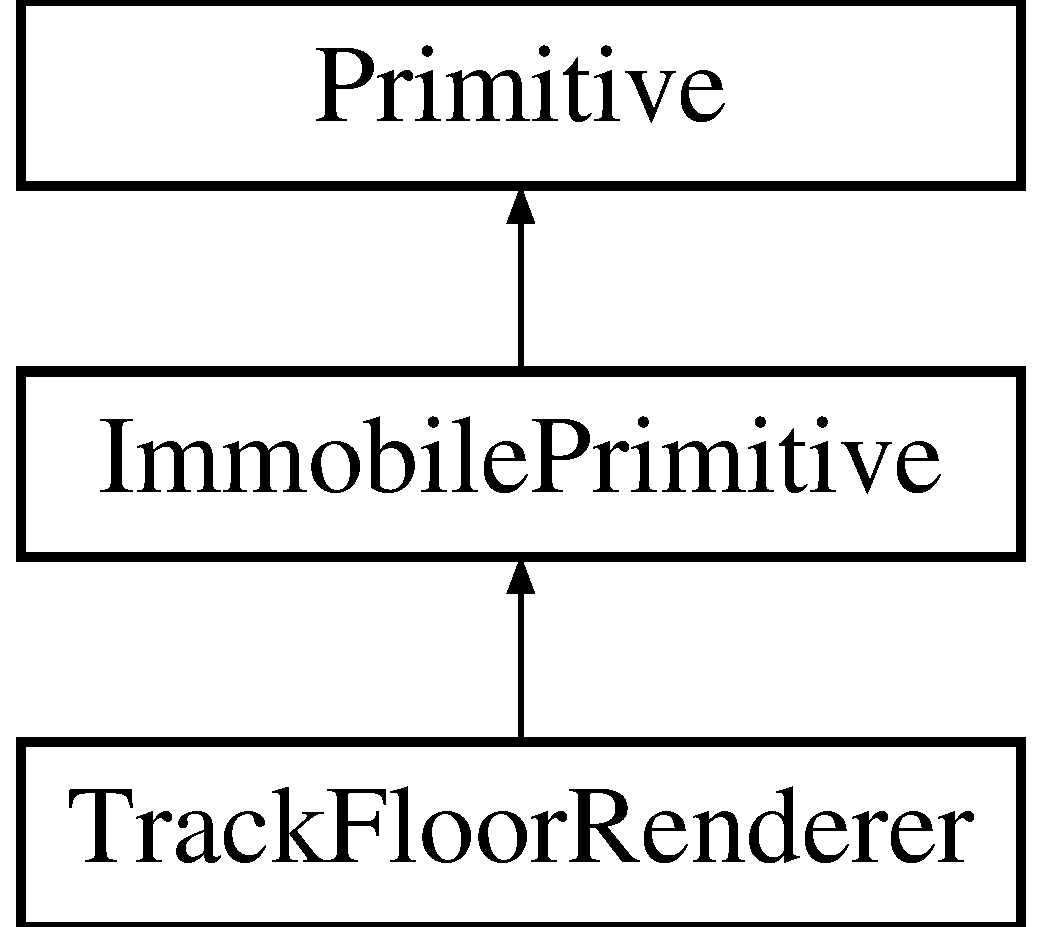
\includegraphics[height=3.000000cm]{class_track_floor_renderer}
\end{center}
\end{figure}
\subsection*{Public Member Functions}
\begin{DoxyCompactItemize}
\item 
\hyperlink{class_track_floor_renderer_a0180ee417454612e322df50801d3b092}{Track\-Floor\-Renderer} (const \hyperlink{class_bezier_patch_grid}{Bezier\-Patch\-Grid} $\ast$bpg, const \hyperlink{class_grid2_d}{Grid2\-D}$<$ \hyperlink{_electric_colour_8hpp_a1979e84576b59c4d100d8a8cc41de734}{E\-\_\-\-E\-L\-E\-C\-T\-R\-I\-C\-C\-O\-L\-O\-U\-R} $>$ $\ast$colourgrid, int cells\-Per\-Patch\-X, int cells\-Per\-Patch\-Y, \hyperlink{class_material}{Material} $\ast$$\ast$materials, \hyperlink{class_texture}{Texture} $\ast$texture, double textures\-Per\-Cell\-X, double textures\-Per\-Cell\-Y)
\item 
\hyperlink{class_track_floor_renderer_aac2d8df7abbc9472c49b9fbfb2221103}{$\sim$\-Track\-Floor\-Renderer} ()
\end{DoxyCompactItemize}
\subsection*{Additional Inherited Members}


\subsection{Constructor \& Destructor Documentation}
\hypertarget{class_track_floor_renderer_a0180ee417454612e322df50801d3b092}{\index{Track\-Floor\-Renderer@{Track\-Floor\-Renderer}!Track\-Floor\-Renderer@{Track\-Floor\-Renderer}}
\index{Track\-Floor\-Renderer@{Track\-Floor\-Renderer}!TrackFloorRenderer@{Track\-Floor\-Renderer}}
\subsubsection[{Track\-Floor\-Renderer}]{\setlength{\rightskip}{0pt plus 5cm}Track\-Floor\-Renderer\-::\-Track\-Floor\-Renderer (
\begin{DoxyParamCaption}
\item[{const {\bf Bezier\-Patch\-Grid} $\ast$}]{bpg, }
\item[{const {\bf Grid2\-D}$<$ {\bf E\-\_\-\-E\-L\-E\-C\-T\-R\-I\-C\-C\-O\-L\-O\-U\-R} $>$ $\ast$}]{colourgrid, }
\item[{int}]{cells\-Per\-Patch\-X, }
\item[{int}]{cells\-Per\-Patch\-Y, }
\item[{{\bf Material} $\ast$$\ast$}]{materials, }
\item[{{\bf Texture} $\ast$}]{texture, }
\item[{double}]{textures\-Per\-Cell\-X, }
\item[{double}]{textures\-Per\-Cell\-Y}
\end{DoxyParamCaption}
)}}\label{class_track_floor_renderer_a0180ee417454612e322df50801d3b092}
\hypertarget{class_track_floor_renderer_aac2d8df7abbc9472c49b9fbfb2221103}{\index{Track\-Floor\-Renderer@{Track\-Floor\-Renderer}!$\sim$\-Track\-Floor\-Renderer@{$\sim$\-Track\-Floor\-Renderer}}
\index{$\sim$\-Track\-Floor\-Renderer@{$\sim$\-Track\-Floor\-Renderer}!TrackFloorRenderer@{Track\-Floor\-Renderer}}
\subsubsection[{$\sim$\-Track\-Floor\-Renderer}]{\setlength{\rightskip}{0pt plus 5cm}Track\-Floor\-Renderer\-::$\sim$\-Track\-Floor\-Renderer (
\begin{DoxyParamCaption}
{}
\end{DoxyParamCaption}
)}}\label{class_track_floor_renderer_aac2d8df7abbc9472c49b9fbfb2221103}


The documentation for this class was generated from the following files\-:\begin{DoxyCompactItemize}
\item 
C\-:/\-Users/\-Owner/\-My Programming/\-Personal Projects/\-Video\-Games/\-Optimist Racing/src/\hyperlink{_primitive_8hpp}{Primitive.\-hpp}\item 
C\-:/\-Users/\-Owner/\-My Programming/\-Personal Projects/\-Video\-Games/\-Optimist Racing/src/\hyperlink{_primitive_8cpp}{Primitive.\-cpp}\end{DoxyCompactItemize}

\hypertarget{class_vector2_d}{\section{Vector2\-D Class Reference}
\label{class_vector2_d}\index{Vector2\-D@{Vector2\-D}}
}


Represents a vector with 2 entries.  




{\ttfamily \#include $<$Algebra.\-hpp$>$}

\subsection*{Public Member Functions}
\begin{DoxyCompactItemize}
\item 
\hyperlink{class_vector2_d_a98e9997ebb7a629f4db52397d4e0d653}{Vector2\-D} ()
\begin{DoxyCompactList}\small\item\em Makes a zero vector. \end{DoxyCompactList}\item 
\hyperlink{class_vector2_d_a525e125aac4c844f04c52ddb0e75d594}{Vector2\-D} (double x, double y)
\begin{DoxyCompactList}\small\item\em Makes a vector with the entries x and y. \end{DoxyCompactList}\item 
\hyperlink{class_vector2_d_a1d9d4e0b040eab0369eec29401b31046}{Vector2\-D} (const \hyperlink{class_vector2_d}{Vector2\-D} \&other)
\begin{DoxyCompactList}\small\item\em Makes a copy of the vector {\itshape other}. \end{DoxyCompactList}\item 
\hyperlink{class_vector2_d}{Vector2\-D} \& \hyperlink{class_vector2_d_a4fd6b530394125b8ece087531140a1fc}{operator=} (const \hyperlink{class_vector2_d}{Vector2\-D} \&other)
\begin{DoxyCompactList}\small\item\em Makes a copy of the vector {\itshape other}. \end{DoxyCompactList}\item 
double \& \hyperlink{class_vector2_d_afc8c3b48321e523c08c0ce18dd19574c}{operator\mbox{[}$\,$\mbox{]}} (size\-\_\-t idx)
\item 
double \hyperlink{class_vector2_d_ab60ef575eb35a7b4b62629a8cf58a2d7}{operator\mbox{[}$\,$\mbox{]}} (size\-\_\-t idx) const 
\item 
double \hyperlink{class_vector2_d_a218abf7d966c08db96f20628bfe826b1}{euclidean\-Norm2} () const 
\item 
double \hyperlink{class_vector2_d_ae079733cfc3d4fe654065ce7f9d74248}{euclidean\-Norm} () const 
\item 
double \hyperlink{class_vector2_d_abfb37d3be83891cb9b4cc21e5a3ab422}{dot} (const \hyperlink{class_vector2_d}{Vector2\-D} \&other) const 
\begin{DoxyCompactList}\small\item\em Returns the dot product between this and {\itshape other}. \end{DoxyCompactList}\item 
bool \hyperlink{class_vector2_d_a3e453a6740502ed6e63b388015adfedd}{normalize} ()
\end{DoxyCompactItemize}


\subsection{Detailed Description}
Represents a vector with 2 entries. 

This class includes some operations that you can do with 2\-D vectors. \begin{DoxyAuthor}{Author}
Claude Richard 
\end{DoxyAuthor}
\begin{DoxyDate}{Date}
2012 
\end{DoxyDate}


\subsection{Constructor \& Destructor Documentation}
\hypertarget{class_vector2_d_a98e9997ebb7a629f4db52397d4e0d653}{\index{Vector2\-D@{Vector2\-D}!Vector2\-D@{Vector2\-D}}
\index{Vector2\-D@{Vector2\-D}!Vector2D@{Vector2\-D}}
\subsubsection[{Vector2\-D}]{\setlength{\rightskip}{0pt plus 5cm}Vector2\-D\-::\-Vector2\-D (
\begin{DoxyParamCaption}
{}
\end{DoxyParamCaption}
)}}\label{class_vector2_d_a98e9997ebb7a629f4db52397d4e0d653}


Makes a zero vector. 

After this constructor is done, both entries in the vector will be zero. \begin{DoxyPostcond}{Postcondition}
Both entries in the vector are zero. 
\end{DoxyPostcond}
\hypertarget{class_vector2_d_a525e125aac4c844f04c52ddb0e75d594}{\index{Vector2\-D@{Vector2\-D}!Vector2\-D@{Vector2\-D}}
\index{Vector2\-D@{Vector2\-D}!Vector2D@{Vector2\-D}}
\subsubsection[{Vector2\-D}]{\setlength{\rightskip}{0pt plus 5cm}Vector2\-D\-::\-Vector2\-D (
\begin{DoxyParamCaption}
\item[{double}]{x, }
\item[{double}]{y}
\end{DoxyParamCaption}
)}}\label{class_vector2_d_a525e125aac4c844f04c52ddb0e75d594}


Makes a vector with the entries x and y. 

After this constructor is done, the entries in the vector will be x and y, in that order. \begin{DoxyPostcond}{Postcondition}
The vector's entries are x and y, in that order. 
\end{DoxyPostcond}

\begin{DoxyParams}{Parameters}
{\em x} & The 1st value in the vector. \\
\hline
{\em y} & The 2nd value in the vector. \\
\hline
\end{DoxyParams}
\hypertarget{class_vector2_d_a1d9d4e0b040eab0369eec29401b31046}{\index{Vector2\-D@{Vector2\-D}!Vector2\-D@{Vector2\-D}}
\index{Vector2\-D@{Vector2\-D}!Vector2D@{Vector2\-D}}
\subsubsection[{Vector2\-D}]{\setlength{\rightskip}{0pt plus 5cm}Vector2\-D\-::\-Vector2\-D (
\begin{DoxyParamCaption}
\item[{const {\bf Vector2\-D} \&}]{other}
\end{DoxyParamCaption}
)}}\label{class_vector2_d_a1d9d4e0b040eab0369eec29401b31046}


Makes a copy of the vector {\itshape other}. 

After this constructor is done, the entries in this will match the entries in the vector {\itshape other}. \begin{DoxyPostcond}{Postcondition}
The entries in this vector match the entries in the vector {\itshape other}. 
\end{DoxyPostcond}

\begin{DoxyParams}{Parameters}
{\em other} & The vector to copy. \\
\hline
\end{DoxyParams}


\subsection{Member Function Documentation}
\hypertarget{class_vector2_d_abfb37d3be83891cb9b4cc21e5a3ab422}{\index{Vector2\-D@{Vector2\-D}!dot@{dot}}
\index{dot@{dot}!Vector2D@{Vector2\-D}}
\subsubsection[{dot}]{\setlength{\rightskip}{0pt plus 5cm}double Vector2\-D\-::dot (
\begin{DoxyParamCaption}
\item[{const {\bf Vector2\-D} \&}]{other}
\end{DoxyParamCaption}
) const}}\label{class_vector2_d_abfb37d3be83891cb9b4cc21e5a3ab422}


Returns the dot product between this and {\itshape other}. 

Computes the dot product $ \overrightarrow{this} \cdot \overrightarrow{other} $. 
\begin{DoxyParams}{Parameters}
{\em other} & The vector to be dot producted with this. \\
\hline
\end{DoxyParams}
\begin{DoxyReturn}{Returns}
The dot product $ \overrightarrow{this} \cdot \overrightarrow{other} $. 
\end{DoxyReturn}
\hypertarget{class_vector2_d_ae079733cfc3d4fe654065ce7f9d74248}{\index{Vector2\-D@{Vector2\-D}!euclidean\-Norm@{euclidean\-Norm}}
\index{euclidean\-Norm@{euclidean\-Norm}!Vector2D@{Vector2\-D}}
\subsubsection[{euclidean\-Norm}]{\setlength{\rightskip}{0pt plus 5cm}double Vector2\-D\-::euclidean\-Norm (
\begin{DoxyParamCaption}
{}
\end{DoxyParamCaption}
) const}}\label{class_vector2_d_ae079733cfc3d4fe654065ce7f9d74248}
\hypertarget{class_vector2_d_a218abf7d966c08db96f20628bfe826b1}{\index{Vector2\-D@{Vector2\-D}!euclidean\-Norm2@{euclidean\-Norm2}}
\index{euclidean\-Norm2@{euclidean\-Norm2}!Vector2D@{Vector2\-D}}
\subsubsection[{euclidean\-Norm2}]{\setlength{\rightskip}{0pt plus 5cm}double Vector2\-D\-::euclidean\-Norm2 (
\begin{DoxyParamCaption}
{}
\end{DoxyParamCaption}
) const}}\label{class_vector2_d_a218abf7d966c08db96f20628bfe826b1}
\hypertarget{class_vector2_d_a3e453a6740502ed6e63b388015adfedd}{\index{Vector2\-D@{Vector2\-D}!normalize@{normalize}}
\index{normalize@{normalize}!Vector2D@{Vector2\-D}}
\subsubsection[{normalize}]{\setlength{\rightskip}{0pt plus 5cm}bool Vector2\-D\-::normalize (
\begin{DoxyParamCaption}
{}
\end{DoxyParamCaption}
)}}\label{class_vector2_d_a3e453a6740502ed6e63b388015adfedd}
\hypertarget{class_vector2_d_a4fd6b530394125b8ece087531140a1fc}{\index{Vector2\-D@{Vector2\-D}!operator=@{operator=}}
\index{operator=@{operator=}!Vector2D@{Vector2\-D}}
\subsubsection[{operator=}]{\setlength{\rightskip}{0pt plus 5cm}{\bf Vector2\-D} \& Vector2\-D\-::operator= (
\begin{DoxyParamCaption}
\item[{const {\bf Vector2\-D} \&}]{other}
\end{DoxyParamCaption}
)}}\label{class_vector2_d_a4fd6b530394125b8ece087531140a1fc}


Makes a copy of the vector {\itshape other}. 

The entries in this vector will be made to match the entries in the vector {\itshape other}. \begin{DoxyPostcond}{Postcondition}
The entries in this vector match the entries in the vector {\itshape other}. 
\end{DoxyPostcond}

\begin{DoxyParams}{Parameters}
{\em other} & The vector to copy. \\
\hline
\end{DoxyParams}
\begin{DoxyReturn}{Returns}
A reference to this. 
\end{DoxyReturn}
\hypertarget{class_vector2_d_afc8c3b48321e523c08c0ce18dd19574c}{\index{Vector2\-D@{Vector2\-D}!operator\mbox{[}$\,$\mbox{]}@{operator[]}}
\index{operator\mbox{[}$\,$\mbox{]}@{operator[]}!Vector2D@{Vector2\-D}}
\subsubsection[{operator[]}]{\setlength{\rightskip}{0pt plus 5cm}double \& Vector2\-D\-::operator\mbox{[}$\,$\mbox{]} (
\begin{DoxyParamCaption}
\item[{size\-\_\-t}]{idx}
\end{DoxyParamCaption}
)}}\label{class_vector2_d_afc8c3b48321e523c08c0ce18dd19574c}
\hypertarget{class_vector2_d_ab60ef575eb35a7b4b62629a8cf58a2d7}{\index{Vector2\-D@{Vector2\-D}!operator\mbox{[}$\,$\mbox{]}@{operator[]}}
\index{operator\mbox{[}$\,$\mbox{]}@{operator[]}!Vector2D@{Vector2\-D}}
\subsubsection[{operator[]}]{\setlength{\rightskip}{0pt plus 5cm}double Vector2\-D\-::operator\mbox{[}$\,$\mbox{]} (
\begin{DoxyParamCaption}
\item[{size\-\_\-t}]{idx}
\end{DoxyParamCaption}
) const}}\label{class_vector2_d_ab60ef575eb35a7b4b62629a8cf58a2d7}


The documentation for this class was generated from the following files\-:\begin{DoxyCompactItemize}
\item 
C\-:/\-Users/\-Owner/\-My Programming/\-Personal Projects/\-Video\-Games/\-Optimist Racing/src/\hyperlink{_algebra_8hpp}{Algebra.\-hpp}\item 
C\-:/\-Users/\-Owner/\-My Programming/\-Personal Projects/\-Video\-Games/\-Optimist Racing/src/\hyperlink{_algebra_8cpp}{Algebra.\-cpp}\end{DoxyCompactItemize}

\hypertarget{class_vector3_d}{\section{Vector3\-D Class Reference}
\label{class_vector3_d}\index{Vector3\-D@{Vector3\-D}}
}


{\ttfamily \#include $<$Algebra.\-hpp$>$}

\subsection*{Public Member Functions}
\begin{DoxyCompactItemize}
\item 
\hyperlink{class_vector3_d_a0b11a8d75da427b27443d8a94d0d296c}{Vector3\-D} ()
\item 
\hyperlink{class_vector3_d_abd851542da40b1168edcad11fa83b7c2}{Vector3\-D} (double x, double y, double z)
\item 
\hyperlink{class_vector3_d_ab44979be6b9bb7b514faa44b1c287eb4}{Vector3\-D} (const \hyperlink{class_vector3_d}{Vector3\-D} \&other)
\item 
\hyperlink{class_vector3_d}{Vector3\-D} \& \hyperlink{class_vector3_d_af08b65a17f2ba541d715507e7d283a54}{operator=} (const \hyperlink{class_vector3_d}{Vector3\-D} \&other)
\item 
double \& \hyperlink{class_vector3_d_a29b51ae3f30747c5f1915dfb6d716263}{operator\mbox{[}$\,$\mbox{]}} (size\-\_\-t idx)
\item 
double \hyperlink{class_vector3_d_a3f0c34fddb342029b92f4edfd47c0136}{operator\mbox{[}$\,$\mbox{]}} (size\-\_\-t idx) const 
\item 
double \hyperlink{class_vector3_d_a0b88126c5cb26b88e9cd240215d51721}{euclidean\-Norm2} () const 
\item 
double \hyperlink{class_vector3_d_a79e5a852ed84bdb0f83a1cc1edcf6d8b}{euclidean\-Norm} () const 
\item 
double \hyperlink{class_vector3_d_adfea481bddc047a5a45454637e2018f9}{dot} (const \hyperlink{class_vector3_d}{Vector3\-D} \&other) const 
\item 
\hyperlink{class_vector3_d}{Vector3\-D} \hyperlink{class_vector3_d_a81310eb5d5bd8d28feff3daf6abae149}{cross} (const \hyperlink{class_vector3_d}{Vector3\-D} \&other) const 
\item 
bool \hyperlink{class_vector3_d_ae123dba26ebffc58cdc3484930179688}{normalize} ()
\end{DoxyCompactItemize}


\subsection{Constructor \& Destructor Documentation}
\hypertarget{class_vector3_d_a0b11a8d75da427b27443d8a94d0d296c}{\index{Vector3\-D@{Vector3\-D}!Vector3\-D@{Vector3\-D}}
\index{Vector3\-D@{Vector3\-D}!Vector3D@{Vector3\-D}}
\subsubsection[{Vector3\-D}]{\setlength{\rightskip}{0pt plus 5cm}Vector3\-D\-::\-Vector3\-D (
\begin{DoxyParamCaption}
{}
\end{DoxyParamCaption}
)}}\label{class_vector3_d_a0b11a8d75da427b27443d8a94d0d296c}
\hypertarget{class_vector3_d_abd851542da40b1168edcad11fa83b7c2}{\index{Vector3\-D@{Vector3\-D}!Vector3\-D@{Vector3\-D}}
\index{Vector3\-D@{Vector3\-D}!Vector3D@{Vector3\-D}}
\subsubsection[{Vector3\-D}]{\setlength{\rightskip}{0pt plus 5cm}Vector3\-D\-::\-Vector3\-D (
\begin{DoxyParamCaption}
\item[{double}]{x, }
\item[{double}]{y, }
\item[{double}]{z}
\end{DoxyParamCaption}
)}}\label{class_vector3_d_abd851542da40b1168edcad11fa83b7c2}
\hypertarget{class_vector3_d_ab44979be6b9bb7b514faa44b1c287eb4}{\index{Vector3\-D@{Vector3\-D}!Vector3\-D@{Vector3\-D}}
\index{Vector3\-D@{Vector3\-D}!Vector3D@{Vector3\-D}}
\subsubsection[{Vector3\-D}]{\setlength{\rightskip}{0pt plus 5cm}Vector3\-D\-::\-Vector3\-D (
\begin{DoxyParamCaption}
\item[{const {\bf Vector3\-D} \&}]{other}
\end{DoxyParamCaption}
)}}\label{class_vector3_d_ab44979be6b9bb7b514faa44b1c287eb4}


\subsection{Member Function Documentation}
\hypertarget{class_vector3_d_a81310eb5d5bd8d28feff3daf6abae149}{\index{Vector3\-D@{Vector3\-D}!cross@{cross}}
\index{cross@{cross}!Vector3D@{Vector3\-D}}
\subsubsection[{cross}]{\setlength{\rightskip}{0pt plus 5cm}{\bf Vector3\-D} Vector3\-D\-::cross (
\begin{DoxyParamCaption}
\item[{const {\bf Vector3\-D} \&}]{other}
\end{DoxyParamCaption}
) const}}\label{class_vector3_d_a81310eb5d5bd8d28feff3daf6abae149}
\hypertarget{class_vector3_d_adfea481bddc047a5a45454637e2018f9}{\index{Vector3\-D@{Vector3\-D}!dot@{dot}}
\index{dot@{dot}!Vector3D@{Vector3\-D}}
\subsubsection[{dot}]{\setlength{\rightskip}{0pt plus 5cm}double Vector3\-D\-::dot (
\begin{DoxyParamCaption}
\item[{const {\bf Vector3\-D} \&}]{other}
\end{DoxyParamCaption}
) const}}\label{class_vector3_d_adfea481bddc047a5a45454637e2018f9}
\hypertarget{class_vector3_d_a79e5a852ed84bdb0f83a1cc1edcf6d8b}{\index{Vector3\-D@{Vector3\-D}!euclidean\-Norm@{euclidean\-Norm}}
\index{euclidean\-Norm@{euclidean\-Norm}!Vector3D@{Vector3\-D}}
\subsubsection[{euclidean\-Norm}]{\setlength{\rightskip}{0pt plus 5cm}double Vector3\-D\-::euclidean\-Norm (
\begin{DoxyParamCaption}
{}
\end{DoxyParamCaption}
) const}}\label{class_vector3_d_a79e5a852ed84bdb0f83a1cc1edcf6d8b}
\hypertarget{class_vector3_d_a0b88126c5cb26b88e9cd240215d51721}{\index{Vector3\-D@{Vector3\-D}!euclidean\-Norm2@{euclidean\-Norm2}}
\index{euclidean\-Norm2@{euclidean\-Norm2}!Vector3D@{Vector3\-D}}
\subsubsection[{euclidean\-Norm2}]{\setlength{\rightskip}{0pt plus 5cm}double Vector3\-D\-::euclidean\-Norm2 (
\begin{DoxyParamCaption}
{}
\end{DoxyParamCaption}
) const}}\label{class_vector3_d_a0b88126c5cb26b88e9cd240215d51721}
\hypertarget{class_vector3_d_ae123dba26ebffc58cdc3484930179688}{\index{Vector3\-D@{Vector3\-D}!normalize@{normalize}}
\index{normalize@{normalize}!Vector3D@{Vector3\-D}}
\subsubsection[{normalize}]{\setlength{\rightskip}{0pt plus 5cm}bool Vector3\-D\-::normalize (
\begin{DoxyParamCaption}
{}
\end{DoxyParamCaption}
)}}\label{class_vector3_d_ae123dba26ebffc58cdc3484930179688}
\hypertarget{class_vector3_d_af08b65a17f2ba541d715507e7d283a54}{\index{Vector3\-D@{Vector3\-D}!operator=@{operator=}}
\index{operator=@{operator=}!Vector3D@{Vector3\-D}}
\subsubsection[{operator=}]{\setlength{\rightskip}{0pt plus 5cm}{\bf Vector3\-D} \& Vector3\-D\-::operator= (
\begin{DoxyParamCaption}
\item[{const {\bf Vector3\-D} \&}]{other}
\end{DoxyParamCaption}
)}}\label{class_vector3_d_af08b65a17f2ba541d715507e7d283a54}
\hypertarget{class_vector3_d_a29b51ae3f30747c5f1915dfb6d716263}{\index{Vector3\-D@{Vector3\-D}!operator\mbox{[}$\,$\mbox{]}@{operator[]}}
\index{operator\mbox{[}$\,$\mbox{]}@{operator[]}!Vector3D@{Vector3\-D}}
\subsubsection[{operator[]}]{\setlength{\rightskip}{0pt plus 5cm}double \& Vector3\-D\-::operator\mbox{[}$\,$\mbox{]} (
\begin{DoxyParamCaption}
\item[{size\-\_\-t}]{idx}
\end{DoxyParamCaption}
)}}\label{class_vector3_d_a29b51ae3f30747c5f1915dfb6d716263}
\hypertarget{class_vector3_d_a3f0c34fddb342029b92f4edfd47c0136}{\index{Vector3\-D@{Vector3\-D}!operator\mbox{[}$\,$\mbox{]}@{operator[]}}
\index{operator\mbox{[}$\,$\mbox{]}@{operator[]}!Vector3D@{Vector3\-D}}
\subsubsection[{operator[]}]{\setlength{\rightskip}{0pt plus 5cm}double Vector3\-D\-::operator\mbox{[}$\,$\mbox{]} (
\begin{DoxyParamCaption}
\item[{size\-\_\-t}]{idx}
\end{DoxyParamCaption}
) const}}\label{class_vector3_d_a3f0c34fddb342029b92f4edfd47c0136}


The documentation for this class was generated from the following files\-:\begin{DoxyCompactItemize}
\item 
C\-:/\-Users/\-Owner/\-My Programming/\-Personal Projects/\-Video\-Games/\-Optimist Racing/src/\hyperlink{_algebra_8hpp}{Algebra.\-hpp}\item 
C\-:/\-Users/\-Owner/\-My Programming/\-Personal Projects/\-Video\-Games/\-Optimist Racing/src/\hyperlink{_algebra_8cpp}{Algebra.\-cpp}\end{DoxyCompactItemize}

\hypertarget{class_vector_n_d}{\section{Vector\-N\-D Class Reference}
\label{class_vector_n_d}\index{Vector\-N\-D@{Vector\-N\-D}}
}


{\ttfamily \#include $<$Algebra.\-hpp$>$}

\subsection*{Public Member Functions}
\begin{DoxyCompactItemize}
\item 
\hyperlink{class_vector_n_d_a04bf63cd09f861074f9f12cb8841fe9b}{Vector\-N\-D} (int n)
\item 
\hyperlink{class_vector_n_d_a3fb31d80df22f6c6fb0543b0400dadba}{Vector\-N\-D} (int n, const double $\ast$x)
\item 
\hyperlink{class_vector_n_d_ad34b1d325e217b1176b879e8567d7811}{Vector\-N\-D} (const \hyperlink{class_vector_n_d}{Vector\-N\-D} \&other)
\item 
\hyperlink{class_vector_n_d_a55968fd9a45e35a7fbed4c83cac9f0f3}{$\sim$\-Vector\-N\-D} ()
\item 
\hyperlink{class_vector_n_d}{Vector\-N\-D} \& \hyperlink{class_vector_n_d_af2942aee65afd936668105cb738fc0ad}{operator=} (const \hyperlink{class_vector_n_d}{Vector\-N\-D} \&other)
\item 
int \hyperlink{class_vector_n_d_abdbff005e6ab42f1c4dcfb43bd34f185}{get\-Num} () const 
\item 
double \& \hyperlink{class_vector_n_d_ad28f82215e7d1451dcb56313f29a80d5}{operator\mbox{[}$\,$\mbox{]}} (size\-\_\-t idx)
\item 
double \hyperlink{class_vector_n_d_abc39360878982a7a1f7d1836a28effd7}{operator\mbox{[}$\,$\mbox{]}} (size\-\_\-t idx) const 
\item 
double \hyperlink{class_vector_n_d_ab52f6d230cab5210b96d3e1017a6adea}{euclidean\-Norm2} () const 
\item 
double \hyperlink{class_vector_n_d_abf2d675f51c1265689c8781dd4631cb7}{euclidean\-Norm} () const 
\item 
double \hyperlink{class_vector_n_d_a23a9ef3d8c168a26a365fc1490ec04ef}{dot} (const \hyperlink{class_vector_n_d}{Vector\-N\-D} \&other) const 
\item 
bool \hyperlink{class_vector_n_d_a01b21f6af75960680cb3fb0117f4cb58}{normalize} ()
\end{DoxyCompactItemize}


\subsection{Constructor \& Destructor Documentation}
\hypertarget{class_vector_n_d_a04bf63cd09f861074f9f12cb8841fe9b}{\index{Vector\-N\-D@{Vector\-N\-D}!Vector\-N\-D@{Vector\-N\-D}}
\index{Vector\-N\-D@{Vector\-N\-D}!VectorND@{Vector\-N\-D}}
\subsubsection[{Vector\-N\-D}]{\setlength{\rightskip}{0pt plus 5cm}Vector\-N\-D\-::\-Vector\-N\-D (
\begin{DoxyParamCaption}
\item[{int}]{n}
\end{DoxyParamCaption}
)}}\label{class_vector_n_d_a04bf63cd09f861074f9f12cb8841fe9b}
\hypertarget{class_vector_n_d_a3fb31d80df22f6c6fb0543b0400dadba}{\index{Vector\-N\-D@{Vector\-N\-D}!Vector\-N\-D@{Vector\-N\-D}}
\index{Vector\-N\-D@{Vector\-N\-D}!VectorND@{Vector\-N\-D}}
\subsubsection[{Vector\-N\-D}]{\setlength{\rightskip}{0pt plus 5cm}Vector\-N\-D\-::\-Vector\-N\-D (
\begin{DoxyParamCaption}
\item[{int}]{n, }
\item[{const double $\ast$}]{x}
\end{DoxyParamCaption}
)}}\label{class_vector_n_d_a3fb31d80df22f6c6fb0543b0400dadba}
\hypertarget{class_vector_n_d_ad34b1d325e217b1176b879e8567d7811}{\index{Vector\-N\-D@{Vector\-N\-D}!Vector\-N\-D@{Vector\-N\-D}}
\index{Vector\-N\-D@{Vector\-N\-D}!VectorND@{Vector\-N\-D}}
\subsubsection[{Vector\-N\-D}]{\setlength{\rightskip}{0pt plus 5cm}Vector\-N\-D\-::\-Vector\-N\-D (
\begin{DoxyParamCaption}
\item[{const {\bf Vector\-N\-D} \&}]{other}
\end{DoxyParamCaption}
)}}\label{class_vector_n_d_ad34b1d325e217b1176b879e8567d7811}
\hypertarget{class_vector_n_d_a55968fd9a45e35a7fbed4c83cac9f0f3}{\index{Vector\-N\-D@{Vector\-N\-D}!$\sim$\-Vector\-N\-D@{$\sim$\-Vector\-N\-D}}
\index{$\sim$\-Vector\-N\-D@{$\sim$\-Vector\-N\-D}!VectorND@{Vector\-N\-D}}
\subsubsection[{$\sim$\-Vector\-N\-D}]{\setlength{\rightskip}{0pt plus 5cm}Vector\-N\-D\-::$\sim$\-Vector\-N\-D (
\begin{DoxyParamCaption}
{}
\end{DoxyParamCaption}
)}}\label{class_vector_n_d_a55968fd9a45e35a7fbed4c83cac9f0f3}


\subsection{Member Function Documentation}
\hypertarget{class_vector_n_d_a23a9ef3d8c168a26a365fc1490ec04ef}{\index{Vector\-N\-D@{Vector\-N\-D}!dot@{dot}}
\index{dot@{dot}!VectorND@{Vector\-N\-D}}
\subsubsection[{dot}]{\setlength{\rightskip}{0pt plus 5cm}double Vector\-N\-D\-::dot (
\begin{DoxyParamCaption}
\item[{const {\bf Vector\-N\-D} \&}]{other}
\end{DoxyParamCaption}
) const}}\label{class_vector_n_d_a23a9ef3d8c168a26a365fc1490ec04ef}
\hypertarget{class_vector_n_d_abf2d675f51c1265689c8781dd4631cb7}{\index{Vector\-N\-D@{Vector\-N\-D}!euclidean\-Norm@{euclidean\-Norm}}
\index{euclidean\-Norm@{euclidean\-Norm}!VectorND@{Vector\-N\-D}}
\subsubsection[{euclidean\-Norm}]{\setlength{\rightskip}{0pt plus 5cm}double Vector\-N\-D\-::euclidean\-Norm (
\begin{DoxyParamCaption}
{}
\end{DoxyParamCaption}
) const}}\label{class_vector_n_d_abf2d675f51c1265689c8781dd4631cb7}
\hypertarget{class_vector_n_d_ab52f6d230cab5210b96d3e1017a6adea}{\index{Vector\-N\-D@{Vector\-N\-D}!euclidean\-Norm2@{euclidean\-Norm2}}
\index{euclidean\-Norm2@{euclidean\-Norm2}!VectorND@{Vector\-N\-D}}
\subsubsection[{euclidean\-Norm2}]{\setlength{\rightskip}{0pt plus 5cm}double Vector\-N\-D\-::euclidean\-Norm2 (
\begin{DoxyParamCaption}
{}
\end{DoxyParamCaption}
) const}}\label{class_vector_n_d_ab52f6d230cab5210b96d3e1017a6adea}
\hypertarget{class_vector_n_d_abdbff005e6ab42f1c4dcfb43bd34f185}{\index{Vector\-N\-D@{Vector\-N\-D}!get\-Num@{get\-Num}}
\index{get\-Num@{get\-Num}!VectorND@{Vector\-N\-D}}
\subsubsection[{get\-Num}]{\setlength{\rightskip}{0pt plus 5cm}int Vector\-N\-D\-::get\-Num (
\begin{DoxyParamCaption}
{}
\end{DoxyParamCaption}
) const}}\label{class_vector_n_d_abdbff005e6ab42f1c4dcfb43bd34f185}
\hypertarget{class_vector_n_d_a01b21f6af75960680cb3fb0117f4cb58}{\index{Vector\-N\-D@{Vector\-N\-D}!normalize@{normalize}}
\index{normalize@{normalize}!VectorND@{Vector\-N\-D}}
\subsubsection[{normalize}]{\setlength{\rightskip}{0pt plus 5cm}bool Vector\-N\-D\-::normalize (
\begin{DoxyParamCaption}
{}
\end{DoxyParamCaption}
)}}\label{class_vector_n_d_a01b21f6af75960680cb3fb0117f4cb58}
\hypertarget{class_vector_n_d_af2942aee65afd936668105cb738fc0ad}{\index{Vector\-N\-D@{Vector\-N\-D}!operator=@{operator=}}
\index{operator=@{operator=}!VectorND@{Vector\-N\-D}}
\subsubsection[{operator=}]{\setlength{\rightskip}{0pt plus 5cm}{\bf Vector\-N\-D} \& Vector\-N\-D\-::operator= (
\begin{DoxyParamCaption}
\item[{const {\bf Vector\-N\-D} \&}]{other}
\end{DoxyParamCaption}
)}}\label{class_vector_n_d_af2942aee65afd936668105cb738fc0ad}
\hypertarget{class_vector_n_d_ad28f82215e7d1451dcb56313f29a80d5}{\index{Vector\-N\-D@{Vector\-N\-D}!operator\mbox{[}$\,$\mbox{]}@{operator[]}}
\index{operator\mbox{[}$\,$\mbox{]}@{operator[]}!VectorND@{Vector\-N\-D}}
\subsubsection[{operator[]}]{\setlength{\rightskip}{0pt plus 5cm}double \& Vector\-N\-D\-::operator\mbox{[}$\,$\mbox{]} (
\begin{DoxyParamCaption}
\item[{size\-\_\-t}]{idx}
\end{DoxyParamCaption}
)}}\label{class_vector_n_d_ad28f82215e7d1451dcb56313f29a80d5}
\hypertarget{class_vector_n_d_abc39360878982a7a1f7d1836a28effd7}{\index{Vector\-N\-D@{Vector\-N\-D}!operator\mbox{[}$\,$\mbox{]}@{operator[]}}
\index{operator\mbox{[}$\,$\mbox{]}@{operator[]}!VectorND@{Vector\-N\-D}}
\subsubsection[{operator[]}]{\setlength{\rightskip}{0pt plus 5cm}double Vector\-N\-D\-::operator\mbox{[}$\,$\mbox{]} (
\begin{DoxyParamCaption}
\item[{size\-\_\-t}]{idx}
\end{DoxyParamCaption}
) const}}\label{class_vector_n_d_abc39360878982a7a1f7d1836a28effd7}


The documentation for this class was generated from the following files\-:\begin{DoxyCompactItemize}
\item 
C\-:/\-Users/\-Owner/\-My Programming/\-Personal Projects/\-Video\-Games/\-Optimist Racing/src/\hyperlink{_algebra_8hpp}{Algebra.\-hpp}\item 
C\-:/\-Users/\-Owner/\-My Programming/\-Personal Projects/\-Video\-Games/\-Optimist Racing/src/\hyperlink{_algebra_8cpp}{Algebra.\-cpp}\end{DoxyCompactItemize}

\hypertarget{class_world}{\section{World Class Reference}
\label{class_world}\index{World@{World}}
}


{\ttfamily \#include $<$World.\-hpp$>$}

\subsection*{Public Member Functions}
\begin{DoxyCompactItemize}
\item 
\hyperlink{class_world_aa6f775c07acc00ebb539baa170751f74}{World} (\hyperlink{class_world_data}{World\-Data} \&data)
\item 
\hyperlink{class_world_a8c73fba541a5817fff65147ba47cd827}{$\sim$\-World} ()
\item 
void \hyperlink{class_world_a4ebd4684f45e823d00754f07c5b3b836}{set\-Force\-Right} (int force)
\item 
void \hyperlink{class_world_a30ec2c62d41d6480d0edade3225b0b90}{set\-Force\-Up} (int force)
\item 
void \hyperlink{class_world_a9c31cbe9bcbc5a5228d8c58859789634}{step} (double seconds)
\item 
void \hyperlink{class_world_a9ea86b3faa211bac0cc1f8beec534672}{reset} ()
\item 
void \hyperlink{class_world_afd85e5748adc7522c5d2f4ddd2b75a18}{gl\-Render} () const 
\item 
bool \hyperlink{class_world_a939ed3281b9c754e4f3006c7b0735d7c}{get\-Finished} () const 
\end{DoxyCompactItemize}


\subsection{Constructor \& Destructor Documentation}
\hypertarget{class_world_aa6f775c07acc00ebb539baa170751f74}{\index{World@{World}!World@{World}}
\index{World@{World}!World@{World}}
\subsubsection[{World}]{\setlength{\rightskip}{0pt plus 5cm}World\-::\-World (
\begin{DoxyParamCaption}
\item[{{\bf World\-Data} \&}]{data}
\end{DoxyParamCaption}
)}}\label{class_world_aa6f775c07acc00ebb539baa170751f74}
\hypertarget{class_world_a8c73fba541a5817fff65147ba47cd827}{\index{World@{World}!$\sim$\-World@{$\sim$\-World}}
\index{$\sim$\-World@{$\sim$\-World}!World@{World}}
\subsubsection[{$\sim$\-World}]{\setlength{\rightskip}{0pt plus 5cm}World\-::$\sim$\-World (
\begin{DoxyParamCaption}
{}
\end{DoxyParamCaption}
)}}\label{class_world_a8c73fba541a5817fff65147ba47cd827}


\subsection{Member Function Documentation}
\hypertarget{class_world_a939ed3281b9c754e4f3006c7b0735d7c}{\index{World@{World}!get\-Finished@{get\-Finished}}
\index{get\-Finished@{get\-Finished}!World@{World}}
\subsubsection[{get\-Finished}]{\setlength{\rightskip}{0pt plus 5cm}bool World\-::get\-Finished (
\begin{DoxyParamCaption}
{}
\end{DoxyParamCaption}
) const}}\label{class_world_a939ed3281b9c754e4f3006c7b0735d7c}
\hypertarget{class_world_afd85e5748adc7522c5d2f4ddd2b75a18}{\index{World@{World}!gl\-Render@{gl\-Render}}
\index{gl\-Render@{gl\-Render}!World@{World}}
\subsubsection[{gl\-Render}]{\setlength{\rightskip}{0pt plus 5cm}void World\-::gl\-Render (
\begin{DoxyParamCaption}
{}
\end{DoxyParamCaption}
) const}}\label{class_world_afd85e5748adc7522c5d2f4ddd2b75a18}
\hypertarget{class_world_a9ea86b3faa211bac0cc1f8beec534672}{\index{World@{World}!reset@{reset}}
\index{reset@{reset}!World@{World}}
\subsubsection[{reset}]{\setlength{\rightskip}{0pt plus 5cm}void World\-::reset (
\begin{DoxyParamCaption}
{}
\end{DoxyParamCaption}
)}}\label{class_world_a9ea86b3faa211bac0cc1f8beec534672}
\hypertarget{class_world_a4ebd4684f45e823d00754f07c5b3b836}{\index{World@{World}!set\-Force\-Right@{set\-Force\-Right}}
\index{set\-Force\-Right@{set\-Force\-Right}!World@{World}}
\subsubsection[{set\-Force\-Right}]{\setlength{\rightskip}{0pt plus 5cm}void World\-::set\-Force\-Right (
\begin{DoxyParamCaption}
\item[{int}]{force}
\end{DoxyParamCaption}
)}}\label{class_world_a4ebd4684f45e823d00754f07c5b3b836}
\hypertarget{class_world_a30ec2c62d41d6480d0edade3225b0b90}{\index{World@{World}!set\-Force\-Up@{set\-Force\-Up}}
\index{set\-Force\-Up@{set\-Force\-Up}!World@{World}}
\subsubsection[{set\-Force\-Up}]{\setlength{\rightskip}{0pt plus 5cm}void World\-::set\-Force\-Up (
\begin{DoxyParamCaption}
\item[{int}]{force}
\end{DoxyParamCaption}
)}}\label{class_world_a30ec2c62d41d6480d0edade3225b0b90}
\hypertarget{class_world_a9c31cbe9bcbc5a5228d8c58859789634}{\index{World@{World}!step@{step}}
\index{step@{step}!World@{World}}
\subsubsection[{step}]{\setlength{\rightskip}{0pt plus 5cm}void World\-::step (
\begin{DoxyParamCaption}
\item[{double}]{seconds}
\end{DoxyParamCaption}
)}}\label{class_world_a9c31cbe9bcbc5a5228d8c58859789634}


The documentation for this class was generated from the following files\-:\begin{DoxyCompactItemize}
\item 
C\-:/\-Users/\-Owner/\-My Programming/\-Personal Projects/\-Video\-Games/\-Optimist Racing/src/\hyperlink{_world_8hpp}{World.\-hpp}\item 
C\-:/\-Users/\-Owner/\-My Programming/\-Personal Projects/\-Video\-Games/\-Optimist Racing/src/\hyperlink{_world_8cpp}{World.\-cpp}\end{DoxyCompactItemize}

\hypertarget{class_world_data}{\section{World\-Data Class Reference}
\label{class_world_data}\index{World\-Data@{World\-Data}}
}


{\ttfamily \#include $<$Data.\-hpp$>$}

Inheritance diagram for World\-Data\-:\begin{figure}[H]
\begin{center}
\leavevmode
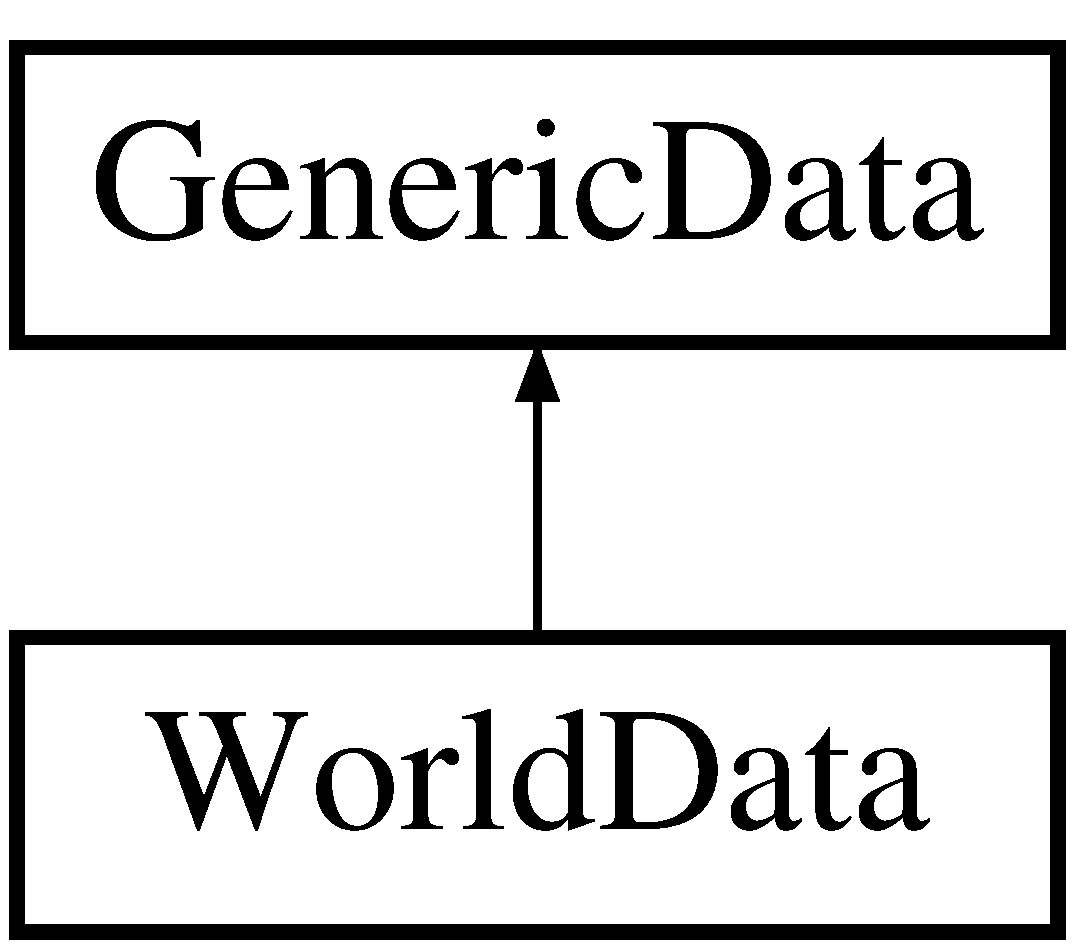
\includegraphics[height=2.000000cm]{class_world_data}
\end{center}
\end{figure}
\subsection*{Public Member Functions}
\begin{DoxyCompactItemize}
\item 
\hyperlink{class_world_data_ad41fc6d2b0c96c6a72569ab32845d342}{World\-Data} (std\-::string filename)
\item 
\hyperlink{class_world_data_abd98753437fa7acfc408d87314b63003}{World\-Data} ()
\item 
\hyperlink{class_world_data_a2a9ddeaaf31f4fcfdd6d0c3ff6d6b2c6}{$\sim$\-World\-Data} ()
\item 
virtual void \hyperlink{class_world_data_aa8a0d950e6d52f7c7baebb722804f55d}{write} (std\-::ostream \&out) const 
\item 
virtual void \hyperlink{class_world_data_aa80956a9e1337417f570f776edeb1c5e}{read} (std\-::istream \&in)
\end{DoxyCompactItemize}
\subsection*{Public Attributes}
\begin{DoxyCompactItemize}
\item 
\hyperlink{class_ambience_render_data}{Ambience\-Render\-Data} \hyperlink{class_world_data_aade26928ad447ef5d3be29828fdd5e75}{m\-Ambience\-Render\-Data}
\item 
\hyperlink{class_floor_data}{Floor\-Data} \hyperlink{class_world_data_a23bdc6fa958c4dca89c6fa60c82e6302}{m\-Floor\-Data}
\item 
\hyperlink{class_floor_render_data}{Floor\-Render\-Data} \hyperlink{class_world_data_a4011d480f1f2c6d7834c0c87b638148f}{m\-Floor\-Render\-Data}
\item 
\hyperlink{class_item_data}{Item\-Data} \hyperlink{class_world_data_ac67d786167b4c19c0f80482039a54bda}{m\-Item\-Data}
\item 
\hyperlink{class_item_render_data}{Item\-Render\-Data} \hyperlink{class_world_data_a5b7cd9727ecd755551f26a5e5ae00401}{m\-Item\-Render\-Data}
\item 
\hyperlink{class_lagrangian_racer_data}{Lagrangian\-Racer\-Data} \hyperlink{class_world_data_af67bbeb4b60eed38f04a58a79e4f1f26}{m\-Lagrangian\-Racer\-Data}
\item 
\hyperlink{class_lagrangian_racer_render_data}{Lagrangian\-Racer\-Render\-Data} \hyperlink{class_world_data_ae5db22573828a345da184d14de38cf6e}{m\-Lagrangian\-Racer\-Render\-Data}
\end{DoxyCompactItemize}


\subsection{Constructor \& Destructor Documentation}
\hypertarget{class_world_data_ad41fc6d2b0c96c6a72569ab32845d342}{\index{World\-Data@{World\-Data}!World\-Data@{World\-Data}}
\index{World\-Data@{World\-Data}!WorldData@{World\-Data}}
\subsubsection[{World\-Data}]{\setlength{\rightskip}{0pt plus 5cm}World\-Data\-::\-World\-Data (
\begin{DoxyParamCaption}
\item[{std\-::string}]{filename}
\end{DoxyParamCaption}
)}}\label{class_world_data_ad41fc6d2b0c96c6a72569ab32845d342}
\hypertarget{class_world_data_abd98753437fa7acfc408d87314b63003}{\index{World\-Data@{World\-Data}!World\-Data@{World\-Data}}
\index{World\-Data@{World\-Data}!WorldData@{World\-Data}}
\subsubsection[{World\-Data}]{\setlength{\rightskip}{0pt plus 5cm}World\-Data\-::\-World\-Data (
\begin{DoxyParamCaption}
{}
\end{DoxyParamCaption}
)}}\label{class_world_data_abd98753437fa7acfc408d87314b63003}
\hypertarget{class_world_data_a2a9ddeaaf31f4fcfdd6d0c3ff6d6b2c6}{\index{World\-Data@{World\-Data}!$\sim$\-World\-Data@{$\sim$\-World\-Data}}
\index{$\sim$\-World\-Data@{$\sim$\-World\-Data}!WorldData@{World\-Data}}
\subsubsection[{$\sim$\-World\-Data}]{\setlength{\rightskip}{0pt plus 5cm}World\-Data\-::$\sim$\-World\-Data (
\begin{DoxyParamCaption}
{}
\end{DoxyParamCaption}
)}}\label{class_world_data_a2a9ddeaaf31f4fcfdd6d0c3ff6d6b2c6}


\subsection{Member Function Documentation}
\hypertarget{class_world_data_aa80956a9e1337417f570f776edeb1c5e}{\index{World\-Data@{World\-Data}!read@{read}}
\index{read@{read}!WorldData@{World\-Data}}
\subsubsection[{read}]{\setlength{\rightskip}{0pt plus 5cm}void World\-Data\-::read (
\begin{DoxyParamCaption}
\item[{std\-::istream \&}]{in}
\end{DoxyParamCaption}
)\hspace{0.3cm}{\ttfamily [virtual]}}}\label{class_world_data_aa80956a9e1337417f570f776edeb1c5e}


Implements \hyperlink{class_generic_data_a71e231ef04c9a91a3429123dab5bd1e7}{Generic\-Data}.

\hypertarget{class_world_data_aa8a0d950e6d52f7c7baebb722804f55d}{\index{World\-Data@{World\-Data}!write@{write}}
\index{write@{write}!WorldData@{World\-Data}}
\subsubsection[{write}]{\setlength{\rightskip}{0pt plus 5cm}void World\-Data\-::write (
\begin{DoxyParamCaption}
\item[{std\-::ostream \&}]{out}
\end{DoxyParamCaption}
) const\hspace{0.3cm}{\ttfamily [virtual]}}}\label{class_world_data_aa8a0d950e6d52f7c7baebb722804f55d}


Implements \hyperlink{class_generic_data_a93ea61de5b09cf3fc95564ef3d841214}{Generic\-Data}.



\subsection{Member Data Documentation}
\hypertarget{class_world_data_aade26928ad447ef5d3be29828fdd5e75}{\index{World\-Data@{World\-Data}!m\-Ambience\-Render\-Data@{m\-Ambience\-Render\-Data}}
\index{m\-Ambience\-Render\-Data@{m\-Ambience\-Render\-Data}!WorldData@{World\-Data}}
\subsubsection[{m\-Ambience\-Render\-Data}]{\setlength{\rightskip}{0pt plus 5cm}{\bf Ambience\-Render\-Data} World\-Data\-::m\-Ambience\-Render\-Data}}\label{class_world_data_aade26928ad447ef5d3be29828fdd5e75}
\hypertarget{class_world_data_a23bdc6fa958c4dca89c6fa60c82e6302}{\index{World\-Data@{World\-Data}!m\-Floor\-Data@{m\-Floor\-Data}}
\index{m\-Floor\-Data@{m\-Floor\-Data}!WorldData@{World\-Data}}
\subsubsection[{m\-Floor\-Data}]{\setlength{\rightskip}{0pt plus 5cm}{\bf Floor\-Data} World\-Data\-::m\-Floor\-Data}}\label{class_world_data_a23bdc6fa958c4dca89c6fa60c82e6302}
\hypertarget{class_world_data_a4011d480f1f2c6d7834c0c87b638148f}{\index{World\-Data@{World\-Data}!m\-Floor\-Render\-Data@{m\-Floor\-Render\-Data}}
\index{m\-Floor\-Render\-Data@{m\-Floor\-Render\-Data}!WorldData@{World\-Data}}
\subsubsection[{m\-Floor\-Render\-Data}]{\setlength{\rightskip}{0pt plus 5cm}{\bf Floor\-Render\-Data} World\-Data\-::m\-Floor\-Render\-Data}}\label{class_world_data_a4011d480f1f2c6d7834c0c87b638148f}
\hypertarget{class_world_data_ac67d786167b4c19c0f80482039a54bda}{\index{World\-Data@{World\-Data}!m\-Item\-Data@{m\-Item\-Data}}
\index{m\-Item\-Data@{m\-Item\-Data}!WorldData@{World\-Data}}
\subsubsection[{m\-Item\-Data}]{\setlength{\rightskip}{0pt plus 5cm}{\bf Item\-Data} World\-Data\-::m\-Item\-Data}}\label{class_world_data_ac67d786167b4c19c0f80482039a54bda}
\hypertarget{class_world_data_a5b7cd9727ecd755551f26a5e5ae00401}{\index{World\-Data@{World\-Data}!m\-Item\-Render\-Data@{m\-Item\-Render\-Data}}
\index{m\-Item\-Render\-Data@{m\-Item\-Render\-Data}!WorldData@{World\-Data}}
\subsubsection[{m\-Item\-Render\-Data}]{\setlength{\rightskip}{0pt plus 5cm}{\bf Item\-Render\-Data} World\-Data\-::m\-Item\-Render\-Data}}\label{class_world_data_a5b7cd9727ecd755551f26a5e5ae00401}
\hypertarget{class_world_data_af67bbeb4b60eed38f04a58a79e4f1f26}{\index{World\-Data@{World\-Data}!m\-Lagrangian\-Racer\-Data@{m\-Lagrangian\-Racer\-Data}}
\index{m\-Lagrangian\-Racer\-Data@{m\-Lagrangian\-Racer\-Data}!WorldData@{World\-Data}}
\subsubsection[{m\-Lagrangian\-Racer\-Data}]{\setlength{\rightskip}{0pt plus 5cm}{\bf Lagrangian\-Racer\-Data} World\-Data\-::m\-Lagrangian\-Racer\-Data}}\label{class_world_data_af67bbeb4b60eed38f04a58a79e4f1f26}
\hypertarget{class_world_data_ae5db22573828a345da184d14de38cf6e}{\index{World\-Data@{World\-Data}!m\-Lagrangian\-Racer\-Render\-Data@{m\-Lagrangian\-Racer\-Render\-Data}}
\index{m\-Lagrangian\-Racer\-Render\-Data@{m\-Lagrangian\-Racer\-Render\-Data}!WorldData@{World\-Data}}
\subsubsection[{m\-Lagrangian\-Racer\-Render\-Data}]{\setlength{\rightskip}{0pt plus 5cm}{\bf Lagrangian\-Racer\-Render\-Data} World\-Data\-::m\-Lagrangian\-Racer\-Render\-Data}}\label{class_world_data_ae5db22573828a345da184d14de38cf6e}


The documentation for this class was generated from the following files\-:\begin{DoxyCompactItemize}
\item 
C\-:/\-Users/\-Owner/\-My Programming/\-Personal Projects/\-Video\-Games/\-Optimist Racing/src/\hyperlink{_data_8hpp}{Data.\-hpp}\item 
C\-:/\-Users/\-Owner/\-My Programming/\-Personal Projects/\-Video\-Games/\-Optimist Racing/src/\hyperlink{_data_8cpp}{Data.\-cpp}\end{DoxyCompactItemize}

\chapter{File Documentation}
\hypertarget{_algebra_8cpp}{\section{C\-:/\-Users/\-Owner/\-My Programming/\-Personal Projects/\-Video\-Games/\-Optimist Racing/src/\-Algebra.cpp File Reference}
\label{_algebra_8cpp}\index{C\-:/\-Users/\-Owner/\-My Programming/\-Personal Projects/\-Video\-Games/\-Optimist Racing/src/\-Algebra.\-cpp@{C\-:/\-Users/\-Owner/\-My Programming/\-Personal Projects/\-Video\-Games/\-Optimist Racing/src/\-Algebra.\-cpp}}
}
{\ttfamily \#include \char`\"{}Algebra.\-hpp\char`\"{}}\\*
\subsection*{Functions}
\begin{DoxyCompactItemize}
\item 
\hyperlink{class_vector2_d}{Vector2\-D} \hyperlink{_algebra_8cpp_ab6d6169dc4d79c3e9ab1dcfefa81abd4}{operator$\ast$} (double s, const \hyperlink{class_vector2_d}{Vector2\-D} \&v)
\item 
\hyperlink{class_vector2_d}{Vector2\-D} \hyperlink{_algebra_8cpp_aa025c19d4e3859ac5cdcdf7301fb31b0}{operator+} (const \hyperlink{class_vector2_d}{Vector2\-D} \&a, const \hyperlink{class_vector2_d}{Vector2\-D} \&b)
\item 
\hyperlink{class_vector2_d}{Vector2\-D} \hyperlink{_algebra_8cpp_ac638052636e6afad1ec34e1bc40610bd}{operator-\/} (const \hyperlink{class_vector2_d}{Vector2\-D} \&a, const \hyperlink{class_vector2_d}{Vector2\-D} \&b)
\item 
\hyperlink{class_vector3_d}{Vector3\-D} \hyperlink{_algebra_8cpp_a82bff392cd419d7f246dfaeb5574ea61}{operator$\ast$} (double s, const \hyperlink{class_vector3_d}{Vector3\-D} \&v)
\item 
\hyperlink{class_vector3_d}{Vector3\-D} \hyperlink{_algebra_8cpp_a39bfe21a2d1ab6984ded35b5355b202e}{operator+} (const \hyperlink{class_vector3_d}{Vector3\-D} \&a, const \hyperlink{class_vector3_d}{Vector3\-D} \&b)
\item 
\hyperlink{class_vector3_d}{Vector3\-D} \hyperlink{_algebra_8cpp_a7ee82807781e470db564c4db6e9de245}{operator-\/} (const \hyperlink{class_vector3_d}{Vector3\-D} \&a, const \hyperlink{class_vector3_d}{Vector3\-D} \&b)
\item 
\hyperlink{class_vector_n_d}{Vector\-N\-D} \hyperlink{_algebra_8cpp_a490c25226403a8aa8c62a29504454fd5}{operator$\ast$} (double s, const \hyperlink{class_vector_n_d}{Vector\-N\-D} \&v)
\item 
\hyperlink{class_vector_n_d}{Vector\-N\-D} \hyperlink{_algebra_8cpp_a40ee5b96e650d2dd80c30bd8be09238c}{operator+} (const \hyperlink{class_vector_n_d}{Vector\-N\-D} \&a, const \hyperlink{class_vector_n_d}{Vector\-N\-D} \&b)
\item 
\hyperlink{class_vector_n_d}{Vector\-N\-D} \hyperlink{_algebra_8cpp_add99f25ed7d4a24a997980bba67ddb1c}{operator-\/} (const \hyperlink{class_vector_n_d}{Vector\-N\-D} \&a, const \hyperlink{class_vector_n_d}{Vector\-N\-D} \&b)
\item 
double \hyperlink{_algebra_8cpp_a17091164dc9b9b93b9d2aafef875dce1}{dot} (const \hyperlink{class_vector2_d}{Vector2\-D} \&a, const \hyperlink{class_vector2_d}{Vector2\-D} \&b)
\item 
double \hyperlink{_algebra_8cpp_a3a8eedd62effe545cfcb0e98651c45e0}{dot} (const \hyperlink{class_vector3_d}{Vector3\-D} \&a, const \hyperlink{class_vector3_d}{Vector3\-D} \&b)
\item 
\hyperlink{class_vector3_d}{Vector3\-D} \hyperlink{_algebra_8cpp_a098c65b80ec865f21eb305b289a9458f}{cross} (const \hyperlink{class_vector3_d}{Vector3\-D} \&a, const \hyperlink{class_vector3_d}{Vector3\-D} \&b)
\item 
\hyperlink{class_matrix2x2}{Matrix2x2} \hyperlink{_algebra_8cpp_a73470dc0e3796ec642f4767bcdd847c6}{operator$\ast$} (const \hyperlink{class_matrix2x2}{Matrix2x2} \&a, const \hyperlink{class_matrix2x2}{Matrix2x2} \&b)
\item 
\hyperlink{class_vector2_d}{Vector2\-D} \hyperlink{_algebra_8cpp_a8d9716d4d0eb7a3f4d9d5ba84552372e}{operator$\ast$} (const \hyperlink{class_matrix2x2}{Matrix2x2} \&a, const \hyperlink{class_vector2_d}{Vector2\-D} \&b)
\item 
\hyperlink{class_vector2_d}{Vector2\-D} \hyperlink{_algebra_8cpp_a8b3ccbbaee2c1326fdf11e543ea759a1}{matrix\-Solve} (const \hyperlink{class_matrix2x2}{Matrix2x2} \&a, const \hyperlink{class_vector2_d}{Vector2\-D} \&b)
\item 
\hyperlink{class_matrix3x3}{Matrix3x3} \hyperlink{_algebra_8cpp_ac5f5320b246b6fd073afce2e66f3e9a3}{operator$\ast$} (const \hyperlink{class_matrix3x3}{Matrix3x3} \&a, const \hyperlink{class_matrix3x3}{Matrix3x3} \&b)
\item 
\hyperlink{class_vector3_d}{Vector3\-D} \hyperlink{_algebra_8cpp_ab164aa4da4ac121cb11231416ebd00b9}{operator$\ast$} (const \hyperlink{class_matrix3x3}{Matrix3x3} \&a, const \hyperlink{class_vector3_d}{Vector3\-D} \&b)
\item 
\hyperlink{class_vector3_d}{Vector3\-D} \hyperlink{_algebra_8cpp_ab3bb244b788a3e6ea44086a6eb93eb18}{matrix\-Solve} (const \hyperlink{class_matrix3x3}{Matrix3x3} \&a, const \hyperlink{class_vector3_d}{Vector3\-D} \&b)
\item 
\hyperlink{class_vector_n_d}{Vector\-N\-D} \hyperlink{_algebra_8cpp_a66bdaf4d1439d9f4423fc4f620cfb494}{operator$\ast$} (const \hyperlink{class_matrix_mx_n}{Matrix\-Mx\-N} \&a, const \hyperlink{class_vector_n_d}{Vector\-N\-D} \&b)
\item 
\hyperlink{class_matrix_mx_n}{Matrix\-Mx\-N} \hyperlink{_algebra_8cpp_a09c94e7fa49cf14ab5dbba439be8d9a0}{operator$\ast$} (double s, const \hyperlink{class_matrix_mx_n}{Matrix\-Mx\-N} \&A)
\item 
double \hyperlink{_algebra_8cpp_a1cd9cc3823a5dfd883a9be42d1904155}{dot} (const \hyperlink{class_matrix_mx_n}{Matrix\-Mx\-N} \&A, const \hyperlink{class_matrix_mx_n}{Matrix\-Mx\-N} \&B)
\end{DoxyCompactItemize}


\subsection{Function Documentation}
\hypertarget{_algebra_8cpp_a098c65b80ec865f21eb305b289a9458f}{\index{Algebra.\-cpp@{Algebra.\-cpp}!cross@{cross}}
\index{cross@{cross}!Algebra.cpp@{Algebra.\-cpp}}
\subsubsection[{cross}]{\setlength{\rightskip}{0pt plus 5cm}{\bf Vector3\-D} cross (
\begin{DoxyParamCaption}
\item[{const {\bf Vector3\-D} \&}]{a, }
\item[{const {\bf Vector3\-D} \&}]{b}
\end{DoxyParamCaption}
)}}\label{_algebra_8cpp_a098c65b80ec865f21eb305b289a9458f}
\hypertarget{_algebra_8cpp_a17091164dc9b9b93b9d2aafef875dce1}{\index{Algebra.\-cpp@{Algebra.\-cpp}!dot@{dot}}
\index{dot@{dot}!Algebra.cpp@{Algebra.\-cpp}}
\subsubsection[{dot}]{\setlength{\rightskip}{0pt plus 5cm}double dot (
\begin{DoxyParamCaption}
\item[{const {\bf Vector2\-D} \&}]{a, }
\item[{const {\bf Vector2\-D} \&}]{b}
\end{DoxyParamCaption}
)}}\label{_algebra_8cpp_a17091164dc9b9b93b9d2aafef875dce1}
\hypertarget{_algebra_8cpp_a3a8eedd62effe545cfcb0e98651c45e0}{\index{Algebra.\-cpp@{Algebra.\-cpp}!dot@{dot}}
\index{dot@{dot}!Algebra.cpp@{Algebra.\-cpp}}
\subsubsection[{dot}]{\setlength{\rightskip}{0pt plus 5cm}double dot (
\begin{DoxyParamCaption}
\item[{const {\bf Vector3\-D} \&}]{a, }
\item[{const {\bf Vector3\-D} \&}]{b}
\end{DoxyParamCaption}
)}}\label{_algebra_8cpp_a3a8eedd62effe545cfcb0e98651c45e0}
\hypertarget{_algebra_8cpp_a1cd9cc3823a5dfd883a9be42d1904155}{\index{Algebra.\-cpp@{Algebra.\-cpp}!dot@{dot}}
\index{dot@{dot}!Algebra.cpp@{Algebra.\-cpp}}
\subsubsection[{dot}]{\setlength{\rightskip}{0pt plus 5cm}double dot (
\begin{DoxyParamCaption}
\item[{const {\bf Matrix\-Mx\-N} \&}]{A, }
\item[{const {\bf Matrix\-Mx\-N} \&}]{B}
\end{DoxyParamCaption}
)}}\label{_algebra_8cpp_a1cd9cc3823a5dfd883a9be42d1904155}
\hypertarget{_algebra_8cpp_a8b3ccbbaee2c1326fdf11e543ea759a1}{\index{Algebra.\-cpp@{Algebra.\-cpp}!matrix\-Solve@{matrix\-Solve}}
\index{matrix\-Solve@{matrix\-Solve}!Algebra.cpp@{Algebra.\-cpp}}
\subsubsection[{matrix\-Solve}]{\setlength{\rightskip}{0pt plus 5cm}{\bf Vector2\-D} matrix\-Solve (
\begin{DoxyParamCaption}
\item[{const {\bf Matrix2x2} \&}]{a, }
\item[{const {\bf Vector2\-D} \&}]{b}
\end{DoxyParamCaption}
)}}\label{_algebra_8cpp_a8b3ccbbaee2c1326fdf11e543ea759a1}
\hypertarget{_algebra_8cpp_ab3bb244b788a3e6ea44086a6eb93eb18}{\index{Algebra.\-cpp@{Algebra.\-cpp}!matrix\-Solve@{matrix\-Solve}}
\index{matrix\-Solve@{matrix\-Solve}!Algebra.cpp@{Algebra.\-cpp}}
\subsubsection[{matrix\-Solve}]{\setlength{\rightskip}{0pt plus 5cm}{\bf Vector3\-D} matrix\-Solve (
\begin{DoxyParamCaption}
\item[{const {\bf Matrix3x3} \&}]{a, }
\item[{const {\bf Vector3\-D} \&}]{b}
\end{DoxyParamCaption}
)}}\label{_algebra_8cpp_ab3bb244b788a3e6ea44086a6eb93eb18}
\hypertarget{_algebra_8cpp_ab6d6169dc4d79c3e9ab1dcfefa81abd4}{\index{Algebra.\-cpp@{Algebra.\-cpp}!operator$\ast$@{operator$\ast$}}
\index{operator$\ast$@{operator$\ast$}!Algebra.cpp@{Algebra.\-cpp}}
\subsubsection[{operator$\ast$}]{\setlength{\rightskip}{0pt plus 5cm}{\bf Vector2\-D} operator$\ast$ (
\begin{DoxyParamCaption}
\item[{double}]{s, }
\item[{const {\bf Vector2\-D} \&}]{v}
\end{DoxyParamCaption}
)}}\label{_algebra_8cpp_ab6d6169dc4d79c3e9ab1dcfefa81abd4}
\hypertarget{_algebra_8cpp_a82bff392cd419d7f246dfaeb5574ea61}{\index{Algebra.\-cpp@{Algebra.\-cpp}!operator$\ast$@{operator$\ast$}}
\index{operator$\ast$@{operator$\ast$}!Algebra.cpp@{Algebra.\-cpp}}
\subsubsection[{operator$\ast$}]{\setlength{\rightskip}{0pt plus 5cm}{\bf Vector3\-D} operator$\ast$ (
\begin{DoxyParamCaption}
\item[{double}]{s, }
\item[{const {\bf Vector3\-D} \&}]{v}
\end{DoxyParamCaption}
)}}\label{_algebra_8cpp_a82bff392cd419d7f246dfaeb5574ea61}
\hypertarget{_algebra_8cpp_a490c25226403a8aa8c62a29504454fd5}{\index{Algebra.\-cpp@{Algebra.\-cpp}!operator$\ast$@{operator$\ast$}}
\index{operator$\ast$@{operator$\ast$}!Algebra.cpp@{Algebra.\-cpp}}
\subsubsection[{operator$\ast$}]{\setlength{\rightskip}{0pt plus 5cm}{\bf Vector\-N\-D} operator$\ast$ (
\begin{DoxyParamCaption}
\item[{double}]{s, }
\item[{const {\bf Vector\-N\-D} \&}]{v}
\end{DoxyParamCaption}
)}}\label{_algebra_8cpp_a490c25226403a8aa8c62a29504454fd5}
\hypertarget{_algebra_8cpp_a73470dc0e3796ec642f4767bcdd847c6}{\index{Algebra.\-cpp@{Algebra.\-cpp}!operator$\ast$@{operator$\ast$}}
\index{operator$\ast$@{operator$\ast$}!Algebra.cpp@{Algebra.\-cpp}}
\subsubsection[{operator$\ast$}]{\setlength{\rightskip}{0pt plus 5cm}{\bf Matrix2x2} operator$\ast$ (
\begin{DoxyParamCaption}
\item[{const {\bf Matrix2x2} \&}]{a, }
\item[{const {\bf Matrix2x2} \&}]{b}
\end{DoxyParamCaption}
)}}\label{_algebra_8cpp_a73470dc0e3796ec642f4767bcdd847c6}
\hypertarget{_algebra_8cpp_a8d9716d4d0eb7a3f4d9d5ba84552372e}{\index{Algebra.\-cpp@{Algebra.\-cpp}!operator$\ast$@{operator$\ast$}}
\index{operator$\ast$@{operator$\ast$}!Algebra.cpp@{Algebra.\-cpp}}
\subsubsection[{operator$\ast$}]{\setlength{\rightskip}{0pt plus 5cm}{\bf Vector2\-D} operator$\ast$ (
\begin{DoxyParamCaption}
\item[{const {\bf Matrix2x2} \&}]{a, }
\item[{const {\bf Vector2\-D} \&}]{b}
\end{DoxyParamCaption}
)}}\label{_algebra_8cpp_a8d9716d4d0eb7a3f4d9d5ba84552372e}
\hypertarget{_algebra_8cpp_ac5f5320b246b6fd073afce2e66f3e9a3}{\index{Algebra.\-cpp@{Algebra.\-cpp}!operator$\ast$@{operator$\ast$}}
\index{operator$\ast$@{operator$\ast$}!Algebra.cpp@{Algebra.\-cpp}}
\subsubsection[{operator$\ast$}]{\setlength{\rightskip}{0pt plus 5cm}{\bf Matrix3x3} operator$\ast$ (
\begin{DoxyParamCaption}
\item[{const {\bf Matrix3x3} \&}]{a, }
\item[{const {\bf Matrix3x3} \&}]{b}
\end{DoxyParamCaption}
)}}\label{_algebra_8cpp_ac5f5320b246b6fd073afce2e66f3e9a3}
\hypertarget{_algebra_8cpp_ab164aa4da4ac121cb11231416ebd00b9}{\index{Algebra.\-cpp@{Algebra.\-cpp}!operator$\ast$@{operator$\ast$}}
\index{operator$\ast$@{operator$\ast$}!Algebra.cpp@{Algebra.\-cpp}}
\subsubsection[{operator$\ast$}]{\setlength{\rightskip}{0pt plus 5cm}{\bf Vector3\-D} operator$\ast$ (
\begin{DoxyParamCaption}
\item[{const {\bf Matrix3x3} \&}]{a, }
\item[{const {\bf Vector3\-D} \&}]{b}
\end{DoxyParamCaption}
)}}\label{_algebra_8cpp_ab164aa4da4ac121cb11231416ebd00b9}
\hypertarget{_algebra_8cpp_a66bdaf4d1439d9f4423fc4f620cfb494}{\index{Algebra.\-cpp@{Algebra.\-cpp}!operator$\ast$@{operator$\ast$}}
\index{operator$\ast$@{operator$\ast$}!Algebra.cpp@{Algebra.\-cpp}}
\subsubsection[{operator$\ast$}]{\setlength{\rightskip}{0pt plus 5cm}{\bf Vector\-N\-D} operator$\ast$ (
\begin{DoxyParamCaption}
\item[{const {\bf Matrix\-Mx\-N} \&}]{a, }
\item[{const {\bf Vector\-N\-D} \&}]{b}
\end{DoxyParamCaption}
)}}\label{_algebra_8cpp_a66bdaf4d1439d9f4423fc4f620cfb494}
\hypertarget{_algebra_8cpp_a09c94e7fa49cf14ab5dbba439be8d9a0}{\index{Algebra.\-cpp@{Algebra.\-cpp}!operator$\ast$@{operator$\ast$}}
\index{operator$\ast$@{operator$\ast$}!Algebra.cpp@{Algebra.\-cpp}}
\subsubsection[{operator$\ast$}]{\setlength{\rightskip}{0pt plus 5cm}{\bf Matrix\-Mx\-N} operator$\ast$ (
\begin{DoxyParamCaption}
\item[{double}]{s, }
\item[{const {\bf Matrix\-Mx\-N} \&}]{A}
\end{DoxyParamCaption}
)}}\label{_algebra_8cpp_a09c94e7fa49cf14ab5dbba439be8d9a0}
\hypertarget{_algebra_8cpp_aa025c19d4e3859ac5cdcdf7301fb31b0}{\index{Algebra.\-cpp@{Algebra.\-cpp}!operator+@{operator+}}
\index{operator+@{operator+}!Algebra.cpp@{Algebra.\-cpp}}
\subsubsection[{operator+}]{\setlength{\rightskip}{0pt plus 5cm}{\bf Vector2\-D} operator+ (
\begin{DoxyParamCaption}
\item[{const {\bf Vector2\-D} \&}]{a, }
\item[{const {\bf Vector2\-D} \&}]{b}
\end{DoxyParamCaption}
)}}\label{_algebra_8cpp_aa025c19d4e3859ac5cdcdf7301fb31b0}
\hypertarget{_algebra_8cpp_a39bfe21a2d1ab6984ded35b5355b202e}{\index{Algebra.\-cpp@{Algebra.\-cpp}!operator+@{operator+}}
\index{operator+@{operator+}!Algebra.cpp@{Algebra.\-cpp}}
\subsubsection[{operator+}]{\setlength{\rightskip}{0pt plus 5cm}{\bf Vector3\-D} operator+ (
\begin{DoxyParamCaption}
\item[{const {\bf Vector3\-D} \&}]{a, }
\item[{const {\bf Vector3\-D} \&}]{b}
\end{DoxyParamCaption}
)}}\label{_algebra_8cpp_a39bfe21a2d1ab6984ded35b5355b202e}
\hypertarget{_algebra_8cpp_a40ee5b96e650d2dd80c30bd8be09238c}{\index{Algebra.\-cpp@{Algebra.\-cpp}!operator+@{operator+}}
\index{operator+@{operator+}!Algebra.cpp@{Algebra.\-cpp}}
\subsubsection[{operator+}]{\setlength{\rightskip}{0pt plus 5cm}{\bf Vector\-N\-D} operator+ (
\begin{DoxyParamCaption}
\item[{const {\bf Vector\-N\-D} \&}]{a, }
\item[{const {\bf Vector\-N\-D} \&}]{b}
\end{DoxyParamCaption}
)}}\label{_algebra_8cpp_a40ee5b96e650d2dd80c30bd8be09238c}
\hypertarget{_algebra_8cpp_ac638052636e6afad1ec34e1bc40610bd}{\index{Algebra.\-cpp@{Algebra.\-cpp}!operator-\/@{operator-\/}}
\index{operator-\/@{operator-\/}!Algebra.cpp@{Algebra.\-cpp}}
\subsubsection[{operator-\/}]{\setlength{\rightskip}{0pt plus 5cm}{\bf Vector2\-D} operator-\/ (
\begin{DoxyParamCaption}
\item[{const {\bf Vector2\-D} \&}]{a, }
\item[{const {\bf Vector2\-D} \&}]{b}
\end{DoxyParamCaption}
)}}\label{_algebra_8cpp_ac638052636e6afad1ec34e1bc40610bd}
\hypertarget{_algebra_8cpp_a7ee82807781e470db564c4db6e9de245}{\index{Algebra.\-cpp@{Algebra.\-cpp}!operator-\/@{operator-\/}}
\index{operator-\/@{operator-\/}!Algebra.cpp@{Algebra.\-cpp}}
\subsubsection[{operator-\/}]{\setlength{\rightskip}{0pt plus 5cm}{\bf Vector3\-D} operator-\/ (
\begin{DoxyParamCaption}
\item[{const {\bf Vector3\-D} \&}]{a, }
\item[{const {\bf Vector3\-D} \&}]{b}
\end{DoxyParamCaption}
)}}\label{_algebra_8cpp_a7ee82807781e470db564c4db6e9de245}
\hypertarget{_algebra_8cpp_add99f25ed7d4a24a997980bba67ddb1c}{\index{Algebra.\-cpp@{Algebra.\-cpp}!operator-\/@{operator-\/}}
\index{operator-\/@{operator-\/}!Algebra.cpp@{Algebra.\-cpp}}
\subsubsection[{operator-\/}]{\setlength{\rightskip}{0pt plus 5cm}{\bf Vector\-N\-D} operator-\/ (
\begin{DoxyParamCaption}
\item[{const {\bf Vector\-N\-D} \&}]{a, }
\item[{const {\bf Vector\-N\-D} \&}]{b}
\end{DoxyParamCaption}
)}}\label{_algebra_8cpp_add99f25ed7d4a24a997980bba67ddb1c}

\hypertarget{_algebra_8hpp}{\section{C\-:/\-Users/\-Owner/\-My Programming/\-Personal Projects/\-Video\-Games/\-Optimist Racing/src/\-Algebra.hpp File Reference}
\label{_algebra_8hpp}\index{C\-:/\-Users/\-Owner/\-My Programming/\-Personal Projects/\-Video\-Games/\-Optimist Racing/src/\-Algebra.\-hpp@{C\-:/\-Users/\-Owner/\-My Programming/\-Personal Projects/\-Video\-Games/\-Optimist Racing/src/\-Algebra.\-hpp}}
}
{\ttfamily \#include $<$algorithm$>$}\\*
{\ttfamily \#include $<$cmath$>$}\\*
\subsection*{Classes}
\begin{DoxyCompactItemize}
\item 
class \hyperlink{class_vector2_d}{Vector2\-D}
\begin{DoxyCompactList}\small\item\em Represents a vector with 2 entries. \end{DoxyCompactList}\item 
class \hyperlink{class_matrix2x2}{Matrix2x2}
\item 
class \hyperlink{class_vector3_d}{Vector3\-D}
\item 
class \hyperlink{class_matrix3x3}{Matrix3x3}
\item 
class \hyperlink{class_vector_n_d}{Vector\-N\-D}
\item 
class \hyperlink{class_matrix_mx_n}{Matrix\-Mx\-N}
\end{DoxyCompactItemize}
\subsection*{Macros}
\begin{DoxyCompactItemize}
\item 
\#define \hyperlink{_algebra_8hpp_ae71449b1cc6e6250b91f539153a7a0d3}{M\-\_\-\-P\-I}~3.\-141592653589793
\end{DoxyCompactItemize}
\subsection*{Functions}
\begin{DoxyCompactItemize}
\item 
\hyperlink{class_vector2_d}{Vector2\-D} \hyperlink{_algebra_8hpp_ab6d6169dc4d79c3e9ab1dcfefa81abd4}{operator$\ast$} (double s, const \hyperlink{class_vector2_d}{Vector2\-D} \&v)
\item 
\hyperlink{class_vector2_d}{Vector2\-D} \hyperlink{_algebra_8hpp_aa025c19d4e3859ac5cdcdf7301fb31b0}{operator+} (const \hyperlink{class_vector2_d}{Vector2\-D} \&a, const \hyperlink{class_vector2_d}{Vector2\-D} \&b)
\item 
\hyperlink{class_vector2_d}{Vector2\-D} \hyperlink{_algebra_8hpp_ac638052636e6afad1ec34e1bc40610bd}{operator-\/} (const \hyperlink{class_vector2_d}{Vector2\-D} \&a, const \hyperlink{class_vector2_d}{Vector2\-D} \&b)
\item 
\hyperlink{class_vector3_d}{Vector3\-D} \hyperlink{_algebra_8hpp_a82bff392cd419d7f246dfaeb5574ea61}{operator$\ast$} (double s, const \hyperlink{class_vector3_d}{Vector3\-D} \&v)
\item 
\hyperlink{class_vector3_d}{Vector3\-D} \hyperlink{_algebra_8hpp_a39bfe21a2d1ab6984ded35b5355b202e}{operator+} (const \hyperlink{class_vector3_d}{Vector3\-D} \&a, const \hyperlink{class_vector3_d}{Vector3\-D} \&b)
\item 
\hyperlink{class_vector3_d}{Vector3\-D} \hyperlink{_algebra_8hpp_a7ee82807781e470db564c4db6e9de245}{operator-\/} (const \hyperlink{class_vector3_d}{Vector3\-D} \&a, const \hyperlink{class_vector3_d}{Vector3\-D} \&b)
\item 
\hyperlink{class_vector_n_d}{Vector\-N\-D} \hyperlink{_algebra_8hpp_a490c25226403a8aa8c62a29504454fd5}{operator$\ast$} (double s, const \hyperlink{class_vector_n_d}{Vector\-N\-D} \&v)
\item 
\hyperlink{class_vector_n_d}{Vector\-N\-D} \hyperlink{_algebra_8hpp_a40ee5b96e650d2dd80c30bd8be09238c}{operator+} (const \hyperlink{class_vector_n_d}{Vector\-N\-D} \&a, const \hyperlink{class_vector_n_d}{Vector\-N\-D} \&b)
\item 
\hyperlink{class_vector_n_d}{Vector\-N\-D} \hyperlink{_algebra_8hpp_add99f25ed7d4a24a997980bba67ddb1c}{operator-\/} (const \hyperlink{class_vector_n_d}{Vector\-N\-D} \&a, const \hyperlink{class_vector_n_d}{Vector\-N\-D} \&b)
\item 
double \hyperlink{_algebra_8hpp_a17091164dc9b9b93b9d2aafef875dce1}{dot} (const \hyperlink{class_vector2_d}{Vector2\-D} \&a, const \hyperlink{class_vector2_d}{Vector2\-D} \&b)
\item 
double \hyperlink{_algebra_8hpp_a3a8eedd62effe545cfcb0e98651c45e0}{dot} (const \hyperlink{class_vector3_d}{Vector3\-D} \&a, const \hyperlink{class_vector3_d}{Vector3\-D} \&b)
\item 
\hyperlink{class_vector3_d}{Vector3\-D} \hyperlink{_algebra_8hpp_a098c65b80ec865f21eb305b289a9458f}{cross} (const \hyperlink{class_vector3_d}{Vector3\-D} \&a, const \hyperlink{class_vector3_d}{Vector3\-D} \&b)
\item 
\hyperlink{class_matrix2x2}{Matrix2x2} \hyperlink{_algebra_8hpp_ac7f5a00cf0b50e36dffeb5946dccc060}{operator$\ast$} (const \hyperlink{class_matrix2x2}{Matrix2x2} \&A, const \hyperlink{class_matrix2x2}{Matrix2x2} \&B)
\item 
\hyperlink{class_vector2_d}{Vector2\-D} \hyperlink{_algebra_8hpp_a91e4603c7fef646c55fda731ec600847}{operator$\ast$} (const \hyperlink{class_matrix2x2}{Matrix2x2} \&A, const \hyperlink{class_vector2_d}{Vector2\-D} \&b)
\item 
\hyperlink{class_vector2_d}{Vector2\-D} \hyperlink{_algebra_8hpp_abdc8f046e355c6b6803706610963874b}{matrix\-Solve} (const \hyperlink{class_matrix2x2}{Matrix2x2} \&A, const \hyperlink{class_vector2_d}{Vector2\-D} \&b)
\item 
\hyperlink{class_matrix3x3}{Matrix3x3} \hyperlink{_algebra_8hpp_ad8655643bc00d88e932ba47abf4b7cbe}{operator$\ast$} (const \hyperlink{class_matrix3x3}{Matrix3x3} \&A, const \hyperlink{class_matrix3x3}{Matrix3x3} \&B)
\item 
\hyperlink{class_vector3_d}{Vector3\-D} \hyperlink{_algebra_8hpp_a52370681a2714a1cfd9a849ec121890c}{operator$\ast$} (const \hyperlink{class_matrix3x3}{Matrix3x3} \&A, const \hyperlink{class_vector3_d}{Vector3\-D} \&b)
\item 
\hyperlink{class_vector3_d}{Vector3\-D} \hyperlink{_algebra_8hpp_ab3bb244b788a3e6ea44086a6eb93eb18}{matrix\-Solve} (const \hyperlink{class_matrix3x3}{Matrix3x3} \&a, const \hyperlink{class_vector3_d}{Vector3\-D} \&b)
\item 
\hyperlink{class_vector_n_d}{Vector\-N\-D} \hyperlink{_algebra_8hpp_a9599c941601b157067c4be94d1e623ef}{operator$\ast$} (const \hyperlink{class_matrix_mx_n}{Matrix\-Mx\-N} \&A, const \hyperlink{class_vector_n_d}{Vector\-N\-D} \&b)
\item 
\hyperlink{class_matrix_mx_n}{Matrix\-Mx\-N} \hyperlink{_algebra_8hpp_a09c94e7fa49cf14ab5dbba439be8d9a0}{operator$\ast$} (double s, const \hyperlink{class_matrix_mx_n}{Matrix\-Mx\-N} \&A)
\item 
double \hyperlink{_algebra_8hpp_a1cd9cc3823a5dfd883a9be42d1904155}{dot} (const \hyperlink{class_matrix_mx_n}{Matrix\-Mx\-N} \&A, const \hyperlink{class_matrix_mx_n}{Matrix\-Mx\-N} \&B)
\end{DoxyCompactItemize}


\subsection{Macro Definition Documentation}
\hypertarget{_algebra_8hpp_ae71449b1cc6e6250b91f539153a7a0d3}{\index{Algebra.\-hpp@{Algebra.\-hpp}!M\-\_\-\-P\-I@{M\-\_\-\-P\-I}}
\index{M\-\_\-\-P\-I@{M\-\_\-\-P\-I}!Algebra.hpp@{Algebra.\-hpp}}
\subsubsection[{M\-\_\-\-P\-I}]{\setlength{\rightskip}{0pt plus 5cm}\#define M\-\_\-\-P\-I~3.\-141592653589793}}\label{_algebra_8hpp_ae71449b1cc6e6250b91f539153a7a0d3}
This file contains the code necessary for all sorts of linear algebra, which includes vectors and matrices of varying sizes. 

\subsection{Function Documentation}
\hypertarget{_algebra_8hpp_a098c65b80ec865f21eb305b289a9458f}{\index{Algebra.\-hpp@{Algebra.\-hpp}!cross@{cross}}
\index{cross@{cross}!Algebra.hpp@{Algebra.\-hpp}}
\subsubsection[{cross}]{\setlength{\rightskip}{0pt plus 5cm}{\bf Vector3\-D} cross (
\begin{DoxyParamCaption}
\item[{const {\bf Vector3\-D} \&}]{a, }
\item[{const {\bf Vector3\-D} \&}]{b}
\end{DoxyParamCaption}
)}}\label{_algebra_8hpp_a098c65b80ec865f21eb305b289a9458f}
\hypertarget{_algebra_8hpp_a17091164dc9b9b93b9d2aafef875dce1}{\index{Algebra.\-hpp@{Algebra.\-hpp}!dot@{dot}}
\index{dot@{dot}!Algebra.hpp@{Algebra.\-hpp}}
\subsubsection[{dot}]{\setlength{\rightskip}{0pt plus 5cm}double dot (
\begin{DoxyParamCaption}
\item[{const {\bf Vector2\-D} \&}]{a, }
\item[{const {\bf Vector2\-D} \&}]{b}
\end{DoxyParamCaption}
)}}\label{_algebra_8hpp_a17091164dc9b9b93b9d2aafef875dce1}
\hypertarget{_algebra_8hpp_a3a8eedd62effe545cfcb0e98651c45e0}{\index{Algebra.\-hpp@{Algebra.\-hpp}!dot@{dot}}
\index{dot@{dot}!Algebra.hpp@{Algebra.\-hpp}}
\subsubsection[{dot}]{\setlength{\rightskip}{0pt plus 5cm}double dot (
\begin{DoxyParamCaption}
\item[{const {\bf Vector3\-D} \&}]{a, }
\item[{const {\bf Vector3\-D} \&}]{b}
\end{DoxyParamCaption}
)}}\label{_algebra_8hpp_a3a8eedd62effe545cfcb0e98651c45e0}
\hypertarget{_algebra_8hpp_a1cd9cc3823a5dfd883a9be42d1904155}{\index{Algebra.\-hpp@{Algebra.\-hpp}!dot@{dot}}
\index{dot@{dot}!Algebra.hpp@{Algebra.\-hpp}}
\subsubsection[{dot}]{\setlength{\rightskip}{0pt plus 5cm}double dot (
\begin{DoxyParamCaption}
\item[{const {\bf Matrix\-Mx\-N} \&}]{A, }
\item[{const {\bf Matrix\-Mx\-N} \&}]{B}
\end{DoxyParamCaption}
)}}\label{_algebra_8hpp_a1cd9cc3823a5dfd883a9be42d1904155}
\hypertarget{_algebra_8hpp_abdc8f046e355c6b6803706610963874b}{\index{Algebra.\-hpp@{Algebra.\-hpp}!matrix\-Solve@{matrix\-Solve}}
\index{matrix\-Solve@{matrix\-Solve}!Algebra.hpp@{Algebra.\-hpp}}
\subsubsection[{matrix\-Solve}]{\setlength{\rightskip}{0pt plus 5cm}{\bf Vector2\-D} matrix\-Solve (
\begin{DoxyParamCaption}
\item[{const {\bf Matrix2x2} \&}]{A, }
\item[{const {\bf Vector2\-D} \&}]{b}
\end{DoxyParamCaption}
)}}\label{_algebra_8hpp_abdc8f046e355c6b6803706610963874b}
\hypertarget{_algebra_8hpp_ab3bb244b788a3e6ea44086a6eb93eb18}{\index{Algebra.\-hpp@{Algebra.\-hpp}!matrix\-Solve@{matrix\-Solve}}
\index{matrix\-Solve@{matrix\-Solve}!Algebra.hpp@{Algebra.\-hpp}}
\subsubsection[{matrix\-Solve}]{\setlength{\rightskip}{0pt plus 5cm}{\bf Vector3\-D} matrix\-Solve (
\begin{DoxyParamCaption}
\item[{const {\bf Matrix3x3} \&}]{a, }
\item[{const {\bf Vector3\-D} \&}]{b}
\end{DoxyParamCaption}
)}}\label{_algebra_8hpp_ab3bb244b788a3e6ea44086a6eb93eb18}
\hypertarget{_algebra_8hpp_ab6d6169dc4d79c3e9ab1dcfefa81abd4}{\index{Algebra.\-hpp@{Algebra.\-hpp}!operator$\ast$@{operator$\ast$}}
\index{operator$\ast$@{operator$\ast$}!Algebra.hpp@{Algebra.\-hpp}}
\subsubsection[{operator$\ast$}]{\setlength{\rightskip}{0pt plus 5cm}{\bf Vector2\-D} operator$\ast$ (
\begin{DoxyParamCaption}
\item[{double}]{s, }
\item[{const {\bf Vector2\-D} \&}]{v}
\end{DoxyParamCaption}
)}}\label{_algebra_8hpp_ab6d6169dc4d79c3e9ab1dcfefa81abd4}
\hypertarget{_algebra_8hpp_a82bff392cd419d7f246dfaeb5574ea61}{\index{Algebra.\-hpp@{Algebra.\-hpp}!operator$\ast$@{operator$\ast$}}
\index{operator$\ast$@{operator$\ast$}!Algebra.hpp@{Algebra.\-hpp}}
\subsubsection[{operator$\ast$}]{\setlength{\rightskip}{0pt plus 5cm}{\bf Vector3\-D} operator$\ast$ (
\begin{DoxyParamCaption}
\item[{double}]{s, }
\item[{const {\bf Vector3\-D} \&}]{v}
\end{DoxyParamCaption}
)}}\label{_algebra_8hpp_a82bff392cd419d7f246dfaeb5574ea61}
\hypertarget{_algebra_8hpp_a490c25226403a8aa8c62a29504454fd5}{\index{Algebra.\-hpp@{Algebra.\-hpp}!operator$\ast$@{operator$\ast$}}
\index{operator$\ast$@{operator$\ast$}!Algebra.hpp@{Algebra.\-hpp}}
\subsubsection[{operator$\ast$}]{\setlength{\rightskip}{0pt plus 5cm}{\bf Vector\-N\-D} operator$\ast$ (
\begin{DoxyParamCaption}
\item[{double}]{s, }
\item[{const {\bf Vector\-N\-D} \&}]{v}
\end{DoxyParamCaption}
)}}\label{_algebra_8hpp_a490c25226403a8aa8c62a29504454fd5}
\hypertarget{_algebra_8hpp_ac7f5a00cf0b50e36dffeb5946dccc060}{\index{Algebra.\-hpp@{Algebra.\-hpp}!operator$\ast$@{operator$\ast$}}
\index{operator$\ast$@{operator$\ast$}!Algebra.hpp@{Algebra.\-hpp}}
\subsubsection[{operator$\ast$}]{\setlength{\rightskip}{0pt plus 5cm}{\bf Matrix2x2} operator$\ast$ (
\begin{DoxyParamCaption}
\item[{const {\bf Matrix2x2} \&}]{A, }
\item[{const {\bf Matrix2x2} \&}]{B}
\end{DoxyParamCaption}
)}}\label{_algebra_8hpp_ac7f5a00cf0b50e36dffeb5946dccc060}
\hypertarget{_algebra_8hpp_a91e4603c7fef646c55fda731ec600847}{\index{Algebra.\-hpp@{Algebra.\-hpp}!operator$\ast$@{operator$\ast$}}
\index{operator$\ast$@{operator$\ast$}!Algebra.hpp@{Algebra.\-hpp}}
\subsubsection[{operator$\ast$}]{\setlength{\rightskip}{0pt plus 5cm}{\bf Vector2\-D} operator$\ast$ (
\begin{DoxyParamCaption}
\item[{const {\bf Matrix2x2} \&}]{A, }
\item[{const {\bf Vector2\-D} \&}]{b}
\end{DoxyParamCaption}
)}}\label{_algebra_8hpp_a91e4603c7fef646c55fda731ec600847}
\hypertarget{_algebra_8hpp_ad8655643bc00d88e932ba47abf4b7cbe}{\index{Algebra.\-hpp@{Algebra.\-hpp}!operator$\ast$@{operator$\ast$}}
\index{operator$\ast$@{operator$\ast$}!Algebra.hpp@{Algebra.\-hpp}}
\subsubsection[{operator$\ast$}]{\setlength{\rightskip}{0pt plus 5cm}{\bf Matrix3x3} operator$\ast$ (
\begin{DoxyParamCaption}
\item[{const {\bf Matrix3x3} \&}]{A, }
\item[{const {\bf Matrix3x3} \&}]{B}
\end{DoxyParamCaption}
)}}\label{_algebra_8hpp_ad8655643bc00d88e932ba47abf4b7cbe}
\hypertarget{_algebra_8hpp_a52370681a2714a1cfd9a849ec121890c}{\index{Algebra.\-hpp@{Algebra.\-hpp}!operator$\ast$@{operator$\ast$}}
\index{operator$\ast$@{operator$\ast$}!Algebra.hpp@{Algebra.\-hpp}}
\subsubsection[{operator$\ast$}]{\setlength{\rightskip}{0pt plus 5cm}{\bf Vector3\-D} operator$\ast$ (
\begin{DoxyParamCaption}
\item[{const {\bf Matrix3x3} \&}]{A, }
\item[{const {\bf Vector3\-D} \&}]{b}
\end{DoxyParamCaption}
)}}\label{_algebra_8hpp_a52370681a2714a1cfd9a849ec121890c}
\hypertarget{_algebra_8hpp_a9599c941601b157067c4be94d1e623ef}{\index{Algebra.\-hpp@{Algebra.\-hpp}!operator$\ast$@{operator$\ast$}}
\index{operator$\ast$@{operator$\ast$}!Algebra.hpp@{Algebra.\-hpp}}
\subsubsection[{operator$\ast$}]{\setlength{\rightskip}{0pt plus 5cm}{\bf Vector\-N\-D} operator$\ast$ (
\begin{DoxyParamCaption}
\item[{const {\bf Matrix\-Mx\-N} \&}]{A, }
\item[{const {\bf Vector\-N\-D} \&}]{b}
\end{DoxyParamCaption}
)}}\label{_algebra_8hpp_a9599c941601b157067c4be94d1e623ef}
\hypertarget{_algebra_8hpp_a09c94e7fa49cf14ab5dbba439be8d9a0}{\index{Algebra.\-hpp@{Algebra.\-hpp}!operator$\ast$@{operator$\ast$}}
\index{operator$\ast$@{operator$\ast$}!Algebra.hpp@{Algebra.\-hpp}}
\subsubsection[{operator$\ast$}]{\setlength{\rightskip}{0pt plus 5cm}{\bf Matrix\-Mx\-N} operator$\ast$ (
\begin{DoxyParamCaption}
\item[{double}]{s, }
\item[{const {\bf Matrix\-Mx\-N} \&}]{A}
\end{DoxyParamCaption}
)}}\label{_algebra_8hpp_a09c94e7fa49cf14ab5dbba439be8d9a0}
\hypertarget{_algebra_8hpp_aa025c19d4e3859ac5cdcdf7301fb31b0}{\index{Algebra.\-hpp@{Algebra.\-hpp}!operator+@{operator+}}
\index{operator+@{operator+}!Algebra.hpp@{Algebra.\-hpp}}
\subsubsection[{operator+}]{\setlength{\rightskip}{0pt plus 5cm}{\bf Vector2\-D} operator+ (
\begin{DoxyParamCaption}
\item[{const {\bf Vector2\-D} \&}]{a, }
\item[{const {\bf Vector2\-D} \&}]{b}
\end{DoxyParamCaption}
)}}\label{_algebra_8hpp_aa025c19d4e3859ac5cdcdf7301fb31b0}
\hypertarget{_algebra_8hpp_a39bfe21a2d1ab6984ded35b5355b202e}{\index{Algebra.\-hpp@{Algebra.\-hpp}!operator+@{operator+}}
\index{operator+@{operator+}!Algebra.hpp@{Algebra.\-hpp}}
\subsubsection[{operator+}]{\setlength{\rightskip}{0pt plus 5cm}{\bf Vector3\-D} operator+ (
\begin{DoxyParamCaption}
\item[{const {\bf Vector3\-D} \&}]{a, }
\item[{const {\bf Vector3\-D} \&}]{b}
\end{DoxyParamCaption}
)}}\label{_algebra_8hpp_a39bfe21a2d1ab6984ded35b5355b202e}
\hypertarget{_algebra_8hpp_a40ee5b96e650d2dd80c30bd8be09238c}{\index{Algebra.\-hpp@{Algebra.\-hpp}!operator+@{operator+}}
\index{operator+@{operator+}!Algebra.hpp@{Algebra.\-hpp}}
\subsubsection[{operator+}]{\setlength{\rightskip}{0pt plus 5cm}{\bf Vector\-N\-D} operator+ (
\begin{DoxyParamCaption}
\item[{const {\bf Vector\-N\-D} \&}]{a, }
\item[{const {\bf Vector\-N\-D} \&}]{b}
\end{DoxyParamCaption}
)}}\label{_algebra_8hpp_a40ee5b96e650d2dd80c30bd8be09238c}
\hypertarget{_algebra_8hpp_ac638052636e6afad1ec34e1bc40610bd}{\index{Algebra.\-hpp@{Algebra.\-hpp}!operator-\/@{operator-\/}}
\index{operator-\/@{operator-\/}!Algebra.hpp@{Algebra.\-hpp}}
\subsubsection[{operator-\/}]{\setlength{\rightskip}{0pt plus 5cm}{\bf Vector2\-D} operator-\/ (
\begin{DoxyParamCaption}
\item[{const {\bf Vector2\-D} \&}]{a, }
\item[{const {\bf Vector2\-D} \&}]{b}
\end{DoxyParamCaption}
)}}\label{_algebra_8hpp_ac638052636e6afad1ec34e1bc40610bd}
\hypertarget{_algebra_8hpp_a7ee82807781e470db564c4db6e9de245}{\index{Algebra.\-hpp@{Algebra.\-hpp}!operator-\/@{operator-\/}}
\index{operator-\/@{operator-\/}!Algebra.hpp@{Algebra.\-hpp}}
\subsubsection[{operator-\/}]{\setlength{\rightskip}{0pt plus 5cm}{\bf Vector3\-D} operator-\/ (
\begin{DoxyParamCaption}
\item[{const {\bf Vector3\-D} \&}]{a, }
\item[{const {\bf Vector3\-D} \&}]{b}
\end{DoxyParamCaption}
)}}\label{_algebra_8hpp_a7ee82807781e470db564c4db6e9de245}
\hypertarget{_algebra_8hpp_add99f25ed7d4a24a997980bba67ddb1c}{\index{Algebra.\-hpp@{Algebra.\-hpp}!operator-\/@{operator-\/}}
\index{operator-\/@{operator-\/}!Algebra.hpp@{Algebra.\-hpp}}
\subsubsection[{operator-\/}]{\setlength{\rightskip}{0pt plus 5cm}{\bf Vector\-N\-D} operator-\/ (
\begin{DoxyParamCaption}
\item[{const {\bf Vector\-N\-D} \&}]{a, }
\item[{const {\bf Vector\-N\-D} \&}]{b}
\end{DoxyParamCaption}
)}}\label{_algebra_8hpp_add99f25ed7d4a24a997980bba67ddb1c}

\hypertarget{_algebra_struct_8hpp}{\section{C\-:/\-Users/\-Owner/\-My Programming/\-Personal Projects/\-Video\-Games/\-Optimist Racing/src/\-Algebra\-Struct.hpp File Reference}
\label{_algebra_struct_8hpp}\index{C\-:/\-Users/\-Owner/\-My Programming/\-Personal Projects/\-Video\-Games/\-Optimist Racing/src/\-Algebra\-Struct.\-hpp@{C\-:/\-Users/\-Owner/\-My Programming/\-Personal Projects/\-Video\-Games/\-Optimist Racing/src/\-Algebra\-Struct.\-hpp}}
}
{\ttfamily \#include \char`\"{}Algebra.\-hpp\char`\"{}}\\*
\subsection*{Classes}
\begin{DoxyCompactItemize}
\item 
struct \hyperlink{struct_matrix1_vector1}{Matrix1\-Vector1}
\begin{DoxyCompactList}\small\item\em This struct holds one \hyperlink{class_matrix_mx_n}{Matrix\-Mx\-N} and one \hyperlink{class_vector_n_d}{Vector\-N\-D}. \end{DoxyCompactList}\end{DoxyCompactItemize}


\subsection{Detailed Description}
This file defines structs that contain matrices and vectors. These structs are intended to be returned from functions where you need to compute several matrices/vectors, but you need to compute them in the same function to avoid repeating some code. 
\hypertarget{_bezier_8cpp}{\section{C\-:/\-Users/\-Owner/\-My Programming/\-Personal Projects/\-Video\-Games/\-Optimist Racing/src/\-Bezier.cpp File Reference}
\label{_bezier_8cpp}\index{C\-:/\-Users/\-Owner/\-My Programming/\-Personal Projects/\-Video\-Games/\-Optimist Racing/src/\-Bezier.\-cpp@{C\-:/\-Users/\-Owner/\-My Programming/\-Personal Projects/\-Video\-Games/\-Optimist Racing/src/\-Bezier.\-cpp}}
}
{\ttfamily \#include \char`\"{}Bezier.\-hpp\char`\"{}}\\*

\hypertarget{_bezier_8hpp}{\section{C\-:/\-Users/\-Owner/\-My Programming/\-Personal Projects/\-Video\-Games/\-Optimist Racing/src/\-Bezier.hpp File Reference}
\label{_bezier_8hpp}\index{C\-:/\-Users/\-Owner/\-My Programming/\-Personal Projects/\-Video\-Games/\-Optimist Racing/src/\-Bezier.\-hpp@{C\-:/\-Users/\-Owner/\-My Programming/\-Personal Projects/\-Video\-Games/\-Optimist Racing/src/\-Bezier.\-hpp}}
}
{\ttfamily \#include \char`\"{}Algebra.\-hpp\char`\"{}}\\*
\subsection*{Classes}
\begin{DoxyCompactItemize}
\item 
class \hyperlink{class_bernstein_polynomial}{Bernstein\-Polynomial}
\item 
class \hyperlink{class_bezier_patch}{Bezier\-Patch}
\item 
class \hyperlink{class_bezier_patch_grid}{Bezier\-Patch\-Grid}
\end{DoxyCompactItemize}

\hypertarget{_calculus_8cpp}{\section{C\-:/\-Users/\-Owner/\-My Programming/\-Personal Projects/\-Video\-Games/\-Optimist Racing/src/\-Calculus.cpp File Reference}
\label{_calculus_8cpp}\index{C\-:/\-Users/\-Owner/\-My Programming/\-Personal Projects/\-Video\-Games/\-Optimist Racing/src/\-Calculus.\-cpp@{C\-:/\-Users/\-Owner/\-My Programming/\-Personal Projects/\-Video\-Games/\-Optimist Racing/src/\-Calculus.\-cpp}}
}

\hypertarget{_calculus_8hpp}{\section{C\-:/\-Users/\-Owner/\-My Programming/\-Personal Projects/\-Video\-Games/\-Optimist Racing/src/\-Calculus.hpp File Reference}
\label{_calculus_8hpp}\index{C\-:/\-Users/\-Owner/\-My Programming/\-Personal Projects/\-Video\-Games/\-Optimist Racing/src/\-Calculus.\-hpp@{C\-:/\-Users/\-Owner/\-My Programming/\-Personal Projects/\-Video\-Games/\-Optimist Racing/src/\-Calculus.\-hpp}}
}

\hypertarget{_camera_8cpp}{\section{C\-:/\-Users/\-Owner/\-My Programming/\-Personal Projects/\-Video\-Games/\-Optimist Racing/src/\-Camera.cpp File Reference}
\label{_camera_8cpp}\index{C\-:/\-Users/\-Owner/\-My Programming/\-Personal Projects/\-Video\-Games/\-Optimist Racing/src/\-Camera.\-cpp@{C\-:/\-Users/\-Owner/\-My Programming/\-Personal Projects/\-Video\-Games/\-Optimist Racing/src/\-Camera.\-cpp}}
}
{\ttfamily \#include \char`\"{}Camera.\-hpp\char`\"{}}\\*
{\ttfamily \#include $<$G\-L\textbackslash{}glew.\-h$>$}\\*
{\ttfamily \#include $<$G\-L\textbackslash{}freeglut.\-h$>$}\\*

\hypertarget{_camera_8hpp}{\section{C\-:/\-Users/\-Owner/\-My Programming/\-Personal Projects/\-Video\-Games/\-Optimist Racing/src/\-Camera.hpp File Reference}
\label{_camera_8hpp}\index{C\-:/\-Users/\-Owner/\-My Programming/\-Personal Projects/\-Video\-Games/\-Optimist Racing/src/\-Camera.\-hpp@{C\-:/\-Users/\-Owner/\-My Programming/\-Personal Projects/\-Video\-Games/\-Optimist Racing/src/\-Camera.\-hpp}}
}
{\ttfamily \#include \char`\"{}Algebra.\-hpp\char`\"{}}\\*
{\ttfamily \#include \char`\"{}Lagrange.\-hpp\char`\"{}}\\*
\subsection*{Classes}
\begin{DoxyCompactItemize}
\item 
class \hyperlink{class_camera}{Camera}
\item 
class \hyperlink{class_racer_camera}{Racer\-Camera}
\begin{DoxyCompactList}\small\item\em This camera will follow a racer from behind. \end{DoxyCompactList}\end{DoxyCompactItemize}

\hypertarget{_collision_8cpp}{\section{C\-:/\-Users/\-Owner/\-My Programming/\-Personal Projects/\-Video\-Games/\-Optimist Racing/src/\-Collision.cpp File Reference}
\label{_collision_8cpp}\index{C\-:/\-Users/\-Owner/\-My Programming/\-Personal Projects/\-Video\-Games/\-Optimist Racing/src/\-Collision.\-cpp@{C\-:/\-Users/\-Owner/\-My Programming/\-Personal Projects/\-Video\-Games/\-Optimist Racing/src/\-Collision.\-cpp}}
}
{\ttfamily \#include \char`\"{}Collision.\-hpp\char`\"{}}\\*

\hypertarget{_collision_8hpp}{\section{C\-:/\-Users/\-Owner/\-My Programming/\-Personal Projects/\-Video\-Games/\-Optimist Racing/src/\-Collision.hpp File Reference}
\label{_collision_8hpp}\index{C\-:/\-Users/\-Owner/\-My Programming/\-Personal Projects/\-Video\-Games/\-Optimist Racing/src/\-Collision.\-hpp@{C\-:/\-Users/\-Owner/\-My Programming/\-Personal Projects/\-Video\-Games/\-Optimist Racing/src/\-Collision.\-hpp}}
}
{\ttfamily \#include \char`\"{}Algebra.\-hpp\char`\"{}}\\*
\subsection*{Classes}
\begin{DoxyCompactItemize}
\item 
class \hyperlink{class_collision}{Collision}
\begin{DoxyCompactList}\small\item\em Contains functions for detecting collisions between shapes. \end{DoxyCompactList}\end{DoxyCompactItemize}

\hypertarget{_data_8cpp}{\section{C\-:/\-Users/\-Owner/\-My Programming/\-Personal Projects/\-Video\-Games/\-Optimist Racing/src/\-Data.cpp File Reference}
\label{_data_8cpp}\index{C\-:/\-Users/\-Owner/\-My Programming/\-Personal Projects/\-Video\-Games/\-Optimist Racing/src/\-Data.\-cpp@{C\-:/\-Users/\-Owner/\-My Programming/\-Personal Projects/\-Video\-Games/\-Optimist Racing/src/\-Data.\-cpp}}
}
{\ttfamily \#include \char`\"{}Data.\-hpp\char`\"{}}\\*
{\ttfamily \#include $<$fstream$>$}\\*
{\ttfamily \#include $<$iostream$>$}\\*
{\ttfamily \#include $<$direct.\-h$>$}\\*
\subsection*{Functions}
\begin{DoxyCompactItemize}
\item 
std\-::ostream \& \hyperlink{_data_8cpp_a579ab9204764c2be49239ab062b5b273}{operator$<$$<$} (std\-::ostream \&out, const \hyperlink{class_generic_data}{Generic\-Data} \&data)
\item 
std\-::istream \& \hyperlink{_data_8cpp_a6822e817c6d8c826bdb759e432bb29d3}{operator$>$$>$} (std\-::istream \&in, \hyperlink{class_generic_data}{Generic\-Data} \&data)
\end{DoxyCompactItemize}


\subsection{Function Documentation}
\hypertarget{_data_8cpp_a579ab9204764c2be49239ab062b5b273}{\index{Data.\-cpp@{Data.\-cpp}!operator$<$$<$@{operator$<$$<$}}
\index{operator$<$$<$@{operator$<$$<$}!Data.cpp@{Data.\-cpp}}
\subsubsection[{operator$<$$<$}]{\setlength{\rightskip}{0pt plus 5cm}std\-::ostream\& operator$<$$<$ (
\begin{DoxyParamCaption}
\item[{std\-::ostream \&}]{out, }
\item[{const {\bf Generic\-Data} \&}]{data}
\end{DoxyParamCaption}
)}}\label{_data_8cpp_a579ab9204764c2be49239ab062b5b273}
\hypertarget{_data_8cpp_a6822e817c6d8c826bdb759e432bb29d3}{\index{Data.\-cpp@{Data.\-cpp}!operator$>$$>$@{operator$>$$>$}}
\index{operator$>$$>$@{operator$>$$>$}!Data.cpp@{Data.\-cpp}}
\subsubsection[{operator$>$$>$}]{\setlength{\rightskip}{0pt plus 5cm}std\-::istream\& operator$>$$>$ (
\begin{DoxyParamCaption}
\item[{std\-::istream \&}]{in, }
\item[{{\bf Generic\-Data} \&}]{data}
\end{DoxyParamCaption}
)}}\label{_data_8cpp_a6822e817c6d8c826bdb759e432bb29d3}

\hypertarget{_data_8hpp}{\section{C\-:/\-Users/\-Owner/\-My Programming/\-Personal Projects/\-Video\-Games/\-Optimist Racing/src/\-Data.hpp File Reference}
\label{_data_8hpp}\index{C\-:/\-Users/\-Owner/\-My Programming/\-Personal Projects/\-Video\-Games/\-Optimist Racing/src/\-Data.\-hpp@{C\-:/\-Users/\-Owner/\-My Programming/\-Personal Projects/\-Video\-Games/\-Optimist Racing/src/\-Data.\-hpp}}
}
{\ttfamily \#include $<$iostream$>$}\\*
{\ttfamily \#include $<$string$>$}\\*
{\ttfamily \#include \char`\"{}Algebra.\-hpp\char`\"{}}\\*
{\ttfamily \#include \char`\"{}Electric\-Colour.\-hpp\char`\"{}}\\*
{\ttfamily \#include \char`\"{}Material.\-hpp\char`\"{}}\\*
\subsection*{Classes}
\begin{DoxyCompactItemize}
\item 
class \hyperlink{class_generic_data}{Generic\-Data}
\item 
class \hyperlink{class_electric_material_data}{Electric\-Material\-Data}
\item 
class \hyperlink{class_floor_data}{Floor\-Data}
\item 
class \hyperlink{class_floor_render_data}{Floor\-Render\-Data}
\item 
class \hyperlink{class_lagrangian_racer_data}{Lagrangian\-Racer\-Data}
\item 
class \hyperlink{class_lagrangian_racer_render_data}{Lagrangian\-Racer\-Render\-Data}
\item 
class \hyperlink{class_ambience_render_data}{Ambience\-Render\-Data}
\item 
class \hyperlink{class_item_data}{Item\-Data}
\item 
class \hyperlink{class_item_render_data}{Item\-Render\-Data}
\item 
class \hyperlink{class_world_data}{World\-Data}
\end{DoxyCompactItemize}
\subsection*{Functions}
\begin{DoxyCompactItemize}
\item 
std\-::ostream \& \hyperlink{_data_8hpp_a579ab9204764c2be49239ab062b5b273}{operator$<$$<$} (std\-::ostream \&out, const \hyperlink{class_generic_data}{Generic\-Data} \&data)
\item 
std\-::istream \& \hyperlink{_data_8hpp_a6822e817c6d8c826bdb759e432bb29d3}{operator$>$$>$} (std\-::istream \&in, \hyperlink{class_generic_data}{Generic\-Data} \&data)
\end{DoxyCompactItemize}


\subsection{Function Documentation}
\hypertarget{_data_8hpp_a579ab9204764c2be49239ab062b5b273}{\index{Data.\-hpp@{Data.\-hpp}!operator$<$$<$@{operator$<$$<$}}
\index{operator$<$$<$@{operator$<$$<$}!Data.hpp@{Data.\-hpp}}
\subsubsection[{operator$<$$<$}]{\setlength{\rightskip}{0pt plus 5cm}std\-::ostream\& operator$<$$<$ (
\begin{DoxyParamCaption}
\item[{std\-::ostream \&}]{out, }
\item[{const {\bf Generic\-Data} \&}]{data}
\end{DoxyParamCaption}
)}}\label{_data_8hpp_a579ab9204764c2be49239ab062b5b273}
\hypertarget{_data_8hpp_a6822e817c6d8c826bdb759e432bb29d3}{\index{Data.\-hpp@{Data.\-hpp}!operator$>$$>$@{operator$>$$>$}}
\index{operator$>$$>$@{operator$>$$>$}!Data.hpp@{Data.\-hpp}}
\subsubsection[{operator$>$$>$}]{\setlength{\rightskip}{0pt plus 5cm}std\-::istream\& operator$>$$>$ (
\begin{DoxyParamCaption}
\item[{std\-::istream \&}]{in, }
\item[{{\bf Generic\-Data} \&}]{data}
\end{DoxyParamCaption}
)}}\label{_data_8hpp_a6822e817c6d8c826bdb759e432bb29d3}

\hypertarget{_documentation_example_8hpp}{\section{C\-:/\-Users/\-Owner/\-My Programming/\-Personal Projects/\-Video\-Games/\-Optimist Racing/src/\-Documentation\-Example.hpp File Reference}
\label{_documentation_example_8hpp}\index{C\-:/\-Users/\-Owner/\-My Programming/\-Personal Projects/\-Video\-Games/\-Optimist Racing/src/\-Documentation\-Example.\-hpp@{C\-:/\-Users/\-Owner/\-My Programming/\-Personal Projects/\-Video\-Games/\-Optimist Racing/src/\-Documentation\-Example.\-hpp}}
}
{\ttfamily \#include $<$algorithm$>$}\\*
{\ttfamily \#include $<$cmath$>$}\\*
\subsection*{Classes}
\begin{DoxyCompactItemize}
\item 
class \hyperlink{class_documentation_example_1_1_some_nice_class}{Documentation\-Example\-::\-Some\-Nice\-Class}
\begin{DoxyCompactList}\small\item\em Pretty nice class. \end{DoxyCompactList}\end{DoxyCompactItemize}
\subsection*{Namespaces}
\begin{DoxyCompactItemize}
\item 
namespace \hyperlink{namespace_documentation_example}{Documentation\-Example}
\end{DoxyCompactItemize}
\subsection*{Macros}
\begin{DoxyCompactItemize}
\item 
\#define \hyperlink{_documentation_example_8hpp_a642eb1bd8b5c5c71d712eff4e1a36463}{W\-H\-A\-T\-T\-H\-E\-H\-E\-L\-L}~55.\-9554
\begin{DoxyCompactList}\small\item\em Pretty nice constant. \end{DoxyCompactList}\end{DoxyCompactItemize}
\subsection*{Functions}
\begin{DoxyCompactItemize}
\item 
double \hyperlink{namespace_documentation_example_a6e99a2263a784f6f8b4d3c7f40c1fa49}{Documentation\-Example\-::function2} (int a, int b)
\begin{DoxyCompactList}\small\item\em Pretty nice function of two integers. \end{DoxyCompactList}\end{DoxyCompactItemize}


\subsection{Macro Definition Documentation}
\hypertarget{_documentation_example_8hpp_a642eb1bd8b5c5c71d712eff4e1a36463}{\index{Documentation\-Example.\-hpp@{Documentation\-Example.\-hpp}!W\-H\-A\-T\-T\-H\-E\-H\-E\-L\-L@{W\-H\-A\-T\-T\-H\-E\-H\-E\-L\-L}}
\index{W\-H\-A\-T\-T\-H\-E\-H\-E\-L\-L@{W\-H\-A\-T\-T\-H\-E\-H\-E\-L\-L}!DocumentationExample.hpp@{Documentation\-Example.\-hpp}}
\subsubsection[{W\-H\-A\-T\-T\-H\-E\-H\-E\-L\-L}]{\setlength{\rightskip}{0pt plus 5cm}\#define W\-H\-A\-T\-T\-H\-E\-H\-E\-L\-L~55.\-9554}}\label{_documentation_example_8hpp_a642eb1bd8b5c5c71d712eff4e1a36463}


Pretty nice constant. 

This constant is used to demonstrate a number of section commands. \begin{DoxyAuthor}{Author}
John Doe 

Jan Doe 
\end{DoxyAuthor}
\begin{DoxyDate}{Date}
2008-\/2019 
\end{DoxyDate}
\begin{DoxyPrecond}{Precondition}
First initialize the system. 
\end{DoxyPrecond}
\begin{DoxyRefDesc}{Bug}
\item[\hyperlink{bug__bug000001}{Bug}]This number is not very accurate. \end{DoxyRefDesc}
\begin{DoxyWarning}{Warning}
Believing this nonsense constant can result in severe confusion. 
\end{DoxyWarning}

\hypertarget{_electric_colour_8cpp}{\section{C\-:/\-Users/\-Owner/\-My Programming/\-Personal Projects/\-Video\-Games/\-Optimist Racing/src/\-Electric\-Colour.cpp File Reference}
\label{_electric_colour_8cpp}\index{C\-:/\-Users/\-Owner/\-My Programming/\-Personal Projects/\-Video\-Games/\-Optimist Racing/src/\-Electric\-Colour.\-cpp@{C\-:/\-Users/\-Owner/\-My Programming/\-Personal Projects/\-Video\-Games/\-Optimist Racing/src/\-Electric\-Colour.\-cpp}}
}
{\ttfamily \#include \char`\"{}Electric\-Colour.\-hpp\char`\"{}}\\*
\subsection*{Macros}
\begin{DoxyCompactItemize}
\item 
\#define \hyperlink{_electric_colour_8cpp_a736150ea86727f1bfd395a3177ec75a1}{C\-H\-A\-R\-\_\-\-B\-L\-A\-C\-K}~'N'
\begin{DoxyCompactList}\small\item\em The character representation of E\-L\-E\-C\-T\-R\-I\-C\-C\-O\-L\-O\-U\-R\-\_\-\-B\-L\-A\-C\-K. \end{DoxyCompactList}\item 
\#define \hyperlink{_electric_colour_8cpp_ae214fcc2bffa747aae01bffe750e1d24}{C\-H\-A\-R\-\_\-\-R\-E\-D}~'R'
\begin{DoxyCompactList}\small\item\em The character representation of E\-L\-E\-C\-T\-R\-I\-C\-C\-O\-L\-O\-U\-R\-\_\-\-R\-E\-D. \end{DoxyCompactList}\item 
\#define \hyperlink{_electric_colour_8cpp_a45e84a038e4755d3c13787c1b8cfa9a5}{C\-H\-A\-R\-\_\-\-G\-R\-E\-E\-N}~'G'
\begin{DoxyCompactList}\small\item\em The character representation of E\-L\-E\-C\-T\-R\-I\-C\-C\-O\-L\-O\-U\-R\-\_\-\-G\-R\-E\-E\-N. \end{DoxyCompactList}\item 
\#define \hyperlink{_electric_colour_8cpp_ae524ba22e237c15657e720471a939d2d}{C\-H\-A\-R\-\_\-\-B\-L\-U\-E}~'B'
\begin{DoxyCompactList}\small\item\em The character representation of E\-L\-E\-C\-T\-R\-I\-C\-C\-O\-L\-O\-U\-R\-\_\-\-B\-L\-U\-E. \end{DoxyCompactList}\item 
\#define \hyperlink{_electric_colour_8cpp_a578a278eb31c962f46a3602146b29567}{C\-H\-A\-R\-\_\-\-Y\-E\-L\-L\-O\-W}~'Y'
\begin{DoxyCompactList}\small\item\em The character representation of E\-L\-E\-C\-T\-R\-I\-C\-C\-O\-L\-O\-U\-R\-\_\-\-Y\-E\-L\-L\-O\-W. \end{DoxyCompactList}\item 
\#define \hyperlink{_electric_colour_8cpp_abfd9fd170657287923c268d48656bb1f}{C\-H\-A\-R\-\_\-\-M\-A\-G\-E\-N\-T\-A}~'M'
\begin{DoxyCompactList}\small\item\em The character representation of E\-L\-E\-C\-T\-R\-I\-C\-C\-O\-L\-O\-U\-R\-\_\-\-M\-A\-G\-E\-N\-T\-A. \end{DoxyCompactList}\item 
\#define \hyperlink{_electric_colour_8cpp_aa24dc1c20c96fc00e9f0485e810b76d5}{C\-H\-A\-R\-\_\-\-C\-Y\-A\-N}~'C'
\begin{DoxyCompactList}\small\item\em The character representation of E\-L\-E\-C\-T\-R\-I\-C\-C\-O\-L\-O\-U\-R\-\_\-\-C\-Y\-A\-N. \end{DoxyCompactList}\item 
\#define \hyperlink{_electric_colour_8cpp_ac457a4028285e93297a4a543a9034e11}{C\-H\-A\-R\-\_\-\-W\-H\-I\-T\-E}~'W'
\begin{DoxyCompactList}\small\item\em The character representation of E\-L\-E\-C\-T\-R\-I\-C\-C\-O\-L\-O\-U\-R\-\_\-\-W\-H\-I\-T\-E. \end{DoxyCompactList}\end{DoxyCompactItemize}
\subsection*{Functions}
\begin{DoxyCompactItemize}
\item 
std\-::ostream \& \hyperlink{_electric_colour_8cpp_af1d4177c474974362dbd0b8bd532f54f}{operator$<$$<$} (std\-::ostream \&out, const \hyperlink{_electric_colour_8hpp_a1979e84576b59c4d100d8a8cc41de734}{E\-\_\-\-E\-L\-E\-C\-T\-R\-I\-C\-C\-O\-L\-O\-U\-R} ecol)
\begin{DoxyCompactList}\small\item\em Outputs the character representation of {\itshape ecol} to {\itshape out}. \end{DoxyCompactList}\item 
std\-::istream \& \hyperlink{_electric_colour_8cpp_a1964467d6938e25d600d61f7f83a31bf}{operator$>$$>$} (std\-::istream \&in, \hyperlink{_electric_colour_8hpp_a1979e84576b59c4d100d8a8cc41de734}{E\-\_\-\-E\-L\-E\-C\-T\-R\-I\-C\-C\-O\-L\-O\-U\-R} \&ecol)
\begin{DoxyCompactList}\small\item\em Reads in the character representation of {\itshape ecol} from {\itshape in}. \end{DoxyCompactList}\item 
\hyperlink{_electric_colour_8hpp_a1979e84576b59c4d100d8a8cc41de734}{E\-\_\-\-E\-L\-E\-C\-T\-R\-I\-C\-C\-O\-L\-O\-U\-R} \hyperlink{_electric_colour_8cpp_a91e81cee67c59cecb311503463c2125d}{operator$\sim$} (\hyperlink{_electric_colour_8hpp_a1979e84576b59c4d100d8a8cc41de734}{E\-\_\-\-E\-L\-E\-C\-T\-R\-I\-C\-C\-O\-L\-O\-U\-R} c)
\begin{DoxyCompactList}\small\item\em Inverts the Electric\-Colour {\itshape c}. \end{DoxyCompactList}\item 
\hyperlink{_electric_colour_8hpp_a1979e84576b59c4d100d8a8cc41de734}{E\-\_\-\-E\-L\-E\-C\-T\-R\-I\-C\-C\-O\-L\-O\-U\-R} \hyperlink{_electric_colour_8cpp_ae4b285ef9e9cdb68cdabeac0b1dab616}{operator\&} (\hyperlink{_electric_colour_8hpp_a1979e84576b59c4d100d8a8cc41de734}{E\-\_\-\-E\-L\-E\-C\-T\-R\-I\-C\-C\-O\-L\-O\-U\-R} c1, \hyperlink{_electric_colour_8hpp_a1979e84576b59c4d100d8a8cc41de734}{E\-\_\-\-E\-L\-E\-C\-T\-R\-I\-C\-C\-O\-L\-O\-U\-R} c2)
\begin{DoxyCompactList}\small\item\em Returns the intersection of two Electric\-Colours. \end{DoxyCompactList}\item 
\hyperlink{_electric_colour_8hpp_a1979e84576b59c4d100d8a8cc41de734}{E\-\_\-\-E\-L\-E\-C\-T\-R\-I\-C\-C\-O\-L\-O\-U\-R} \hyperlink{_electric_colour_8cpp_a6868414f583a0227d1232f9dee611fbb}{operator$|$} (\hyperlink{_electric_colour_8hpp_a1979e84576b59c4d100d8a8cc41de734}{E\-\_\-\-E\-L\-E\-C\-T\-R\-I\-C\-C\-O\-L\-O\-U\-R} c1, \hyperlink{_electric_colour_8hpp_a1979e84576b59c4d100d8a8cc41de734}{E\-\_\-\-E\-L\-E\-C\-T\-R\-I\-C\-C\-O\-L\-O\-U\-R} c2)
\begin{DoxyCompactList}\small\item\em Returns the union of two Electric\-Colours. \end{DoxyCompactList}\item 
\hyperlink{_electric_colour_8hpp_a1979e84576b59c4d100d8a8cc41de734}{E\-\_\-\-E\-L\-E\-C\-T\-R\-I\-C\-C\-O\-L\-O\-U\-R} \hyperlink{_electric_colour_8cpp_a8b80adef6ab9b9cb7cb4f84bbb2011c1}{operator$^\wedge$} (\hyperlink{_electric_colour_8hpp_a1979e84576b59c4d100d8a8cc41de734}{E\-\_\-\-E\-L\-E\-C\-T\-R\-I\-C\-C\-O\-L\-O\-U\-R} c1, \hyperlink{_electric_colour_8hpp_a1979e84576b59c4d100d8a8cc41de734}{E\-\_\-\-E\-L\-E\-C\-T\-R\-I\-C\-C\-O\-L\-O\-U\-R} c2)
\begin{DoxyCompactList}\small\item\em Returns the element-\/wise X\-O\-R of {\itshape c1} and {\itshape c2}. \end{DoxyCompactList}\item 
\hyperlink{_electric_colour_8hpp_a1979e84576b59c4d100d8a8cc41de734}{E\-\_\-\-E\-L\-E\-C\-T\-R\-I\-C\-C\-O\-L\-O\-U\-R} \hyperlink{_electric_colour_8cpp_af273b48501b0de5d9be6396c90e9f550}{operator-\/} (\hyperlink{_electric_colour_8hpp_a1979e84576b59c4d100d8a8cc41de734}{E\-\_\-\-E\-L\-E\-C\-T\-R\-I\-C\-C\-O\-L\-O\-U\-R} c1, \hyperlink{_electric_colour_8hpp_a1979e84576b59c4d100d8a8cc41de734}{E\-\_\-\-E\-L\-E\-C\-T\-R\-I\-C\-C\-O\-L\-O\-U\-R} c2)
\begin{DoxyCompactList}\small\item\em Returns the subtraction of two Electric\-Colours. \end{DoxyCompactList}\item 
bool \hyperlink{_electric_colour_8cpp_a848cdfca5532396af5037dfa4eb45963}{operator!} (\hyperlink{_electric_colour_8hpp_a1979e84576b59c4d100d8a8cc41de734}{E\-\_\-\-E\-L\-E\-C\-T\-R\-I\-C\-C\-O\-L\-O\-U\-R} c)
\begin{DoxyCompactList}\small\item\em Determines whether {\itshape c} is B\-L\-A\-C\-K. \end{DoxyCompactList}\item 
bool \hyperlink{_electric_colour_8cpp_af664e90924bd5a7f58472b1e63b22539}{operator\&\&} (\hyperlink{_electric_colour_8hpp_a1979e84576b59c4d100d8a8cc41de734}{E\-\_\-\-E\-L\-E\-C\-T\-R\-I\-C\-C\-O\-L\-O\-U\-R} c1, \hyperlink{_electric_colour_8hpp_a1979e84576b59c4d100d8a8cc41de734}{E\-\_\-\-E\-L\-E\-C\-T\-R\-I\-C\-C\-O\-L\-O\-U\-R} c2)
\begin{DoxyCompactList}\small\item\em Determines whether {\itshape c1} and {\itshape c2} share a basic colour. \end{DoxyCompactList}\item 
bool \hyperlink{_electric_colour_8cpp_a8562ffdba84f04961059cf5e05f84454}{operator$|$$|$} (\hyperlink{_electric_colour_8hpp_a1979e84576b59c4d100d8a8cc41de734}{E\-\_\-\-E\-L\-E\-C\-T\-R\-I\-C\-C\-O\-L\-O\-U\-R} c1, \hyperlink{_electric_colour_8hpp_a1979e84576b59c4d100d8a8cc41de734}{E\-\_\-\-E\-L\-E\-C\-T\-R\-I\-C\-C\-O\-L\-O\-U\-R} c2)
\begin{DoxyCompactList}\small\item\em Determines whether {\itshape c1} and {\itshape c2} are not both B\-L\-A\-C\-K. \end{DoxyCompactList}\item 
bool \hyperlink{_electric_colour_8cpp_aefec5b7d4bc4397fe898d7c9d11fc695}{operator$<$} (\hyperlink{_electric_colour_8hpp_a1979e84576b59c4d100d8a8cc41de734}{E\-\_\-\-E\-L\-E\-C\-T\-R\-I\-C\-C\-O\-L\-O\-U\-R} c1, \hyperlink{_electric_colour_8hpp_a1979e84576b59c4d100d8a8cc41de734}{E\-\_\-\-E\-L\-E\-C\-T\-R\-I\-C\-C\-O\-L\-O\-U\-R} c2)
\begin{DoxyCompactList}\small\item\em Determines whether {\itshape c1} is a proper subset of {\itshape c2}. \end{DoxyCompactList}\item 
bool \hyperlink{_electric_colour_8cpp_a373043b3c5688d1a8cd65adb2849125a}{operator$<$=} (\hyperlink{_electric_colour_8hpp_a1979e84576b59c4d100d8a8cc41de734}{E\-\_\-\-E\-L\-E\-C\-T\-R\-I\-C\-C\-O\-L\-O\-U\-R} c1, \hyperlink{_electric_colour_8hpp_a1979e84576b59c4d100d8a8cc41de734}{E\-\_\-\-E\-L\-E\-C\-T\-R\-I\-C\-C\-O\-L\-O\-U\-R} c2)
\begin{DoxyCompactList}\small\item\em Determines whether {\itshape c1} is a subset of {\itshape c2}. \end{DoxyCompactList}\item 
bool \hyperlink{_electric_colour_8cpp_ad03bdfc78320f02c613ce4da319d1e06}{operator$>$} (\hyperlink{_electric_colour_8hpp_a1979e84576b59c4d100d8a8cc41de734}{E\-\_\-\-E\-L\-E\-C\-T\-R\-I\-C\-C\-O\-L\-O\-U\-R} c1, \hyperlink{_electric_colour_8hpp_a1979e84576b59c4d100d8a8cc41de734}{E\-\_\-\-E\-L\-E\-C\-T\-R\-I\-C\-C\-O\-L\-O\-U\-R} c2)
\begin{DoxyCompactList}\small\item\em Determines whether {\itshape c1} is a proper superset of {\itshape c2}. \end{DoxyCompactList}\item 
bool \hyperlink{_electric_colour_8cpp_a1e931082bbb2c3bc25699efb44064deb}{operator$>$=} (\hyperlink{_electric_colour_8hpp_a1979e84576b59c4d100d8a8cc41de734}{E\-\_\-\-E\-L\-E\-C\-T\-R\-I\-C\-C\-O\-L\-O\-U\-R} c1, \hyperlink{_electric_colour_8hpp_a1979e84576b59c4d100d8a8cc41de734}{E\-\_\-\-E\-L\-E\-C\-T\-R\-I\-C\-C\-O\-L\-O\-U\-R} c2)
\begin{DoxyCompactList}\small\item\em Determines whether {\itshape c1} is a superset of {\itshape c2}. \end{DoxyCompactList}\end{DoxyCompactItemize}


\subsection{Macro Definition Documentation}
\hypertarget{_electric_colour_8cpp_a736150ea86727f1bfd395a3177ec75a1}{\index{Electric\-Colour.\-cpp@{Electric\-Colour.\-cpp}!C\-H\-A\-R\-\_\-\-B\-L\-A\-C\-K@{C\-H\-A\-R\-\_\-\-B\-L\-A\-C\-K}}
\index{C\-H\-A\-R\-\_\-\-B\-L\-A\-C\-K@{C\-H\-A\-R\-\_\-\-B\-L\-A\-C\-K}!ElectricColour.cpp@{Electric\-Colour.\-cpp}}
\subsubsection[{C\-H\-A\-R\-\_\-\-B\-L\-A\-C\-K}]{\setlength{\rightskip}{0pt plus 5cm}\#define C\-H\-A\-R\-\_\-\-B\-L\-A\-C\-K~'N'}}\label{_electric_colour_8cpp_a736150ea86727f1bfd395a3177ec75a1}


The character representation of E\-L\-E\-C\-T\-R\-I\-C\-C\-O\-L\-O\-U\-R\-\_\-\-B\-L\-A\-C\-K. 

\hypertarget{_electric_colour_8cpp_ae524ba22e237c15657e720471a939d2d}{\index{Electric\-Colour.\-cpp@{Electric\-Colour.\-cpp}!C\-H\-A\-R\-\_\-\-B\-L\-U\-E@{C\-H\-A\-R\-\_\-\-B\-L\-U\-E}}
\index{C\-H\-A\-R\-\_\-\-B\-L\-U\-E@{C\-H\-A\-R\-\_\-\-B\-L\-U\-E}!ElectricColour.cpp@{Electric\-Colour.\-cpp}}
\subsubsection[{C\-H\-A\-R\-\_\-\-B\-L\-U\-E}]{\setlength{\rightskip}{0pt plus 5cm}\#define C\-H\-A\-R\-\_\-\-B\-L\-U\-E~'B'}}\label{_electric_colour_8cpp_ae524ba22e237c15657e720471a939d2d}


The character representation of E\-L\-E\-C\-T\-R\-I\-C\-C\-O\-L\-O\-U\-R\-\_\-\-B\-L\-U\-E. 

\hypertarget{_electric_colour_8cpp_aa24dc1c20c96fc00e9f0485e810b76d5}{\index{Electric\-Colour.\-cpp@{Electric\-Colour.\-cpp}!C\-H\-A\-R\-\_\-\-C\-Y\-A\-N@{C\-H\-A\-R\-\_\-\-C\-Y\-A\-N}}
\index{C\-H\-A\-R\-\_\-\-C\-Y\-A\-N@{C\-H\-A\-R\-\_\-\-C\-Y\-A\-N}!ElectricColour.cpp@{Electric\-Colour.\-cpp}}
\subsubsection[{C\-H\-A\-R\-\_\-\-C\-Y\-A\-N}]{\setlength{\rightskip}{0pt plus 5cm}\#define C\-H\-A\-R\-\_\-\-C\-Y\-A\-N~'C'}}\label{_electric_colour_8cpp_aa24dc1c20c96fc00e9f0485e810b76d5}


The character representation of E\-L\-E\-C\-T\-R\-I\-C\-C\-O\-L\-O\-U\-R\-\_\-\-C\-Y\-A\-N. 

\hypertarget{_electric_colour_8cpp_a45e84a038e4755d3c13787c1b8cfa9a5}{\index{Electric\-Colour.\-cpp@{Electric\-Colour.\-cpp}!C\-H\-A\-R\-\_\-\-G\-R\-E\-E\-N@{C\-H\-A\-R\-\_\-\-G\-R\-E\-E\-N}}
\index{C\-H\-A\-R\-\_\-\-G\-R\-E\-E\-N@{C\-H\-A\-R\-\_\-\-G\-R\-E\-E\-N}!ElectricColour.cpp@{Electric\-Colour.\-cpp}}
\subsubsection[{C\-H\-A\-R\-\_\-\-G\-R\-E\-E\-N}]{\setlength{\rightskip}{0pt plus 5cm}\#define C\-H\-A\-R\-\_\-\-G\-R\-E\-E\-N~'G'}}\label{_electric_colour_8cpp_a45e84a038e4755d3c13787c1b8cfa9a5}


The character representation of E\-L\-E\-C\-T\-R\-I\-C\-C\-O\-L\-O\-U\-R\-\_\-\-G\-R\-E\-E\-N. 

\hypertarget{_electric_colour_8cpp_abfd9fd170657287923c268d48656bb1f}{\index{Electric\-Colour.\-cpp@{Electric\-Colour.\-cpp}!C\-H\-A\-R\-\_\-\-M\-A\-G\-E\-N\-T\-A@{C\-H\-A\-R\-\_\-\-M\-A\-G\-E\-N\-T\-A}}
\index{C\-H\-A\-R\-\_\-\-M\-A\-G\-E\-N\-T\-A@{C\-H\-A\-R\-\_\-\-M\-A\-G\-E\-N\-T\-A}!ElectricColour.cpp@{Electric\-Colour.\-cpp}}
\subsubsection[{C\-H\-A\-R\-\_\-\-M\-A\-G\-E\-N\-T\-A}]{\setlength{\rightskip}{0pt plus 5cm}\#define C\-H\-A\-R\-\_\-\-M\-A\-G\-E\-N\-T\-A~'M'}}\label{_electric_colour_8cpp_abfd9fd170657287923c268d48656bb1f}


The character representation of E\-L\-E\-C\-T\-R\-I\-C\-C\-O\-L\-O\-U\-R\-\_\-\-M\-A\-G\-E\-N\-T\-A. 

\hypertarget{_electric_colour_8cpp_ae214fcc2bffa747aae01bffe750e1d24}{\index{Electric\-Colour.\-cpp@{Electric\-Colour.\-cpp}!C\-H\-A\-R\-\_\-\-R\-E\-D@{C\-H\-A\-R\-\_\-\-R\-E\-D}}
\index{C\-H\-A\-R\-\_\-\-R\-E\-D@{C\-H\-A\-R\-\_\-\-R\-E\-D}!ElectricColour.cpp@{Electric\-Colour.\-cpp}}
\subsubsection[{C\-H\-A\-R\-\_\-\-R\-E\-D}]{\setlength{\rightskip}{0pt plus 5cm}\#define C\-H\-A\-R\-\_\-\-R\-E\-D~'R'}}\label{_electric_colour_8cpp_ae214fcc2bffa747aae01bffe750e1d24}


The character representation of E\-L\-E\-C\-T\-R\-I\-C\-C\-O\-L\-O\-U\-R\-\_\-\-R\-E\-D. 

\hypertarget{_electric_colour_8cpp_ac457a4028285e93297a4a543a9034e11}{\index{Electric\-Colour.\-cpp@{Electric\-Colour.\-cpp}!C\-H\-A\-R\-\_\-\-W\-H\-I\-T\-E@{C\-H\-A\-R\-\_\-\-W\-H\-I\-T\-E}}
\index{C\-H\-A\-R\-\_\-\-W\-H\-I\-T\-E@{C\-H\-A\-R\-\_\-\-W\-H\-I\-T\-E}!ElectricColour.cpp@{Electric\-Colour.\-cpp}}
\subsubsection[{C\-H\-A\-R\-\_\-\-W\-H\-I\-T\-E}]{\setlength{\rightskip}{0pt plus 5cm}\#define C\-H\-A\-R\-\_\-\-W\-H\-I\-T\-E~'W'}}\label{_electric_colour_8cpp_ac457a4028285e93297a4a543a9034e11}


The character representation of E\-L\-E\-C\-T\-R\-I\-C\-C\-O\-L\-O\-U\-R\-\_\-\-W\-H\-I\-T\-E. 

\hypertarget{_electric_colour_8cpp_a578a278eb31c962f46a3602146b29567}{\index{Electric\-Colour.\-cpp@{Electric\-Colour.\-cpp}!C\-H\-A\-R\-\_\-\-Y\-E\-L\-L\-O\-W@{C\-H\-A\-R\-\_\-\-Y\-E\-L\-L\-O\-W}}
\index{C\-H\-A\-R\-\_\-\-Y\-E\-L\-L\-O\-W@{C\-H\-A\-R\-\_\-\-Y\-E\-L\-L\-O\-W}!ElectricColour.cpp@{Electric\-Colour.\-cpp}}
\subsubsection[{C\-H\-A\-R\-\_\-\-Y\-E\-L\-L\-O\-W}]{\setlength{\rightskip}{0pt plus 5cm}\#define C\-H\-A\-R\-\_\-\-Y\-E\-L\-L\-O\-W~'Y'}}\label{_electric_colour_8cpp_a578a278eb31c962f46a3602146b29567}


The character representation of E\-L\-E\-C\-T\-R\-I\-C\-C\-O\-L\-O\-U\-R\-\_\-\-Y\-E\-L\-L\-O\-W. 



\subsection{Function Documentation}
\hypertarget{_electric_colour_8cpp_a848cdfca5532396af5037dfa4eb45963}{\index{Electric\-Colour.\-cpp@{Electric\-Colour.\-cpp}!operator!@{operator!}}
\index{operator!@{operator!}!ElectricColour.cpp@{Electric\-Colour.\-cpp}}
\subsubsection[{operator!}]{\setlength{\rightskip}{0pt plus 5cm}bool operator! (
\begin{DoxyParamCaption}
\item[{{\bf E\-\_\-\-E\-L\-E\-C\-T\-R\-I\-C\-C\-O\-L\-O\-U\-R}}]{c}
\end{DoxyParamCaption}
)}}\label{_electric_colour_8cpp_a848cdfca5532396af5037dfa4eb45963}


Determines whether {\itshape c} is B\-L\-A\-C\-K. 

Each Electric\-Colour represents a subset of the set \{red, green, blue\}. This function returns true if and only if {\itshape c} is the empty set, i.\-e. B\-L\-A\-C\-K. 
\begin{DoxyParams}{Parameters}
{\em c} & The Electric\-Colour that may or may not be B\-L\-A\-C\-K. \\
\hline
\end{DoxyParams}
\begin{DoxyReturn}{Returns}
True if and only if {\itshape c} is B\-L\-A\-C\-K. 
\end{DoxyReturn}
\hypertarget{_electric_colour_8cpp_ae4b285ef9e9cdb68cdabeac0b1dab616}{\index{Electric\-Colour.\-cpp@{Electric\-Colour.\-cpp}!operator\&@{operator\&}}
\index{operator\&@{operator\&}!ElectricColour.cpp@{Electric\-Colour.\-cpp}}
\subsubsection[{operator\&}]{\setlength{\rightskip}{0pt plus 5cm}{\bf E\-\_\-\-E\-L\-E\-C\-T\-R\-I\-C\-C\-O\-L\-O\-U\-R} operator\& (
\begin{DoxyParamCaption}
\item[{{\bf E\-\_\-\-E\-L\-E\-C\-T\-R\-I\-C\-C\-O\-L\-O\-U\-R}}]{c1, }
\item[{{\bf E\-\_\-\-E\-L\-E\-C\-T\-R\-I\-C\-C\-O\-L\-O\-U\-R}}]{c2}
\end{DoxyParamCaption}
)}}\label{_electric_colour_8cpp_ae4b285ef9e9cdb68cdabeac0b1dab616}


Returns the intersection of two Electric\-Colours. 

Each Electric\-Colour represents a subset of the set \{red, green, blue\}. This function returns an Electric\-Colour representing the intersection of the two arguments. 
\begin{DoxyParams}{Parameters}
{\em c1} & The first Electric\-Colour. \\
\hline
{\em c2} & The second Electric\-Colour. \\
\hline
\end{DoxyParams}
\begin{DoxyReturn}{Returns}
The intersection of {\itshape c1} and {\itshape c2}. 
\end{DoxyReturn}
\hypertarget{_electric_colour_8cpp_af664e90924bd5a7f58472b1e63b22539}{\index{Electric\-Colour.\-cpp@{Electric\-Colour.\-cpp}!operator\&\&@{operator\&\&}}
\index{operator\&\&@{operator\&\&}!ElectricColour.cpp@{Electric\-Colour.\-cpp}}
\subsubsection[{operator\&\&}]{\setlength{\rightskip}{0pt plus 5cm}bool operator\&\& (
\begin{DoxyParamCaption}
\item[{{\bf E\-\_\-\-E\-L\-E\-C\-T\-R\-I\-C\-C\-O\-L\-O\-U\-R}}]{c1, }
\item[{{\bf E\-\_\-\-E\-L\-E\-C\-T\-R\-I\-C\-C\-O\-L\-O\-U\-R}}]{c2}
\end{DoxyParamCaption}
)}}\label{_electric_colour_8cpp_af664e90924bd5a7f58472b1e63b22539}


Determines whether {\itshape c1} and {\itshape c2} share a basic colour. 

Each Electric\-Colour represents a subset of the set \{red, green, blue\}. This function returns true if and only if there exists a basic colour which is in both {\itshape c1} and {\itshape c2}. 
\begin{DoxyParams}{Parameters}
{\em c1} & The first Electric\-Colour. \\
\hline
{\em c2} & The second Electric\-Colour. \\
\hline
\end{DoxyParams}
\begin{DoxyReturn}{Returns}
True if and only if {\itshape c1} and {\itshape c2} share a basic colour. 
\end{DoxyReturn}
\hypertarget{_electric_colour_8cpp_af273b48501b0de5d9be6396c90e9f550}{\index{Electric\-Colour.\-cpp@{Electric\-Colour.\-cpp}!operator-\/@{operator-\/}}
\index{operator-\/@{operator-\/}!ElectricColour.cpp@{Electric\-Colour.\-cpp}}
\subsubsection[{operator-\/}]{\setlength{\rightskip}{0pt plus 5cm}{\bf E\-\_\-\-E\-L\-E\-C\-T\-R\-I\-C\-C\-O\-L\-O\-U\-R} operator-\/ (
\begin{DoxyParamCaption}
\item[{{\bf E\-\_\-\-E\-L\-E\-C\-T\-R\-I\-C\-C\-O\-L\-O\-U\-R}}]{c1, }
\item[{{\bf E\-\_\-\-E\-L\-E\-C\-T\-R\-I\-C\-C\-O\-L\-O\-U\-R}}]{c2}
\end{DoxyParamCaption}
)}}\label{_electric_colour_8cpp_af273b48501b0de5d9be6396c90e9f550}


Returns the subtraction of two Electric\-Colours. 

Each Electric\-Colour represents a subset of the set \{red, green, blue\}. This function returns an Electric\-Colour representing the subtraction of the two arguments. In other words, it returns an Electric\-Colour c3 such that for each basic colour c in \{red, green, blue\}, c3 contains c if and only if c1 contains c and c2 doesn't contain c. 
\begin{DoxyParams}{Parameters}
{\em c1} & The first Electric\-Colour. \\
\hline
{\em c2} & The second Electric\-Colour. \\
\hline
\end{DoxyParams}
\begin{DoxyReturn}{Returns}
The subtraction of {\itshape c1} and {\itshape c2}. 
\end{DoxyReturn}
\hypertarget{_electric_colour_8cpp_aefec5b7d4bc4397fe898d7c9d11fc695}{\index{Electric\-Colour.\-cpp@{Electric\-Colour.\-cpp}!operator$<$@{operator$<$}}
\index{operator$<$@{operator$<$}!ElectricColour.cpp@{Electric\-Colour.\-cpp}}
\subsubsection[{operator$<$}]{\setlength{\rightskip}{0pt plus 5cm}bool operator$<$ (
\begin{DoxyParamCaption}
\item[{{\bf E\-\_\-\-E\-L\-E\-C\-T\-R\-I\-C\-C\-O\-L\-O\-U\-R}}]{c1, }
\item[{{\bf E\-\_\-\-E\-L\-E\-C\-T\-R\-I\-C\-C\-O\-L\-O\-U\-R}}]{c2}
\end{DoxyParamCaption}
)}}\label{_electric_colour_8cpp_aefec5b7d4bc4397fe898d7c9d11fc695}


Determines whether {\itshape c1} is a proper subset of {\itshape c2}. 

Each Electric\-Colour represents a subset of the set \{red, green, blue\}. This function returns true if and only if c2 contains every basic colour that c1 contains and c1 contains strictly fewer basic colours than c2. 
\begin{DoxyParams}{Parameters}
{\em c1} & The Electric\-Colour that may or may not be a proper subset of {\itshape c2}. \\
\hline
{\em c2} & The Electric\-Colour that may or may not be a proper superset of {\itshape c1}. \\
\hline
\end{DoxyParams}
\begin{DoxyReturn}{Returns}
True if and only if {\itshape c1} is a proper subset of {\itshape c2}. 
\end{DoxyReturn}
\hypertarget{_electric_colour_8cpp_af1d4177c474974362dbd0b8bd532f54f}{\index{Electric\-Colour.\-cpp@{Electric\-Colour.\-cpp}!operator$<$$<$@{operator$<$$<$}}
\index{operator$<$$<$@{operator$<$$<$}!ElectricColour.cpp@{Electric\-Colour.\-cpp}}
\subsubsection[{operator$<$$<$}]{\setlength{\rightskip}{0pt plus 5cm}std\-::ostream\& operator$<$$<$ (
\begin{DoxyParamCaption}
\item[{std\-::ostream \&}]{out, }
\item[{const {\bf E\-\_\-\-E\-L\-E\-C\-T\-R\-I\-C\-C\-O\-L\-O\-U\-R}}]{ecol}
\end{DoxyParamCaption}
)}}\label{_electric_colour_8cpp_af1d4177c474974362dbd0b8bd532f54f}


Outputs the character representation of {\itshape ecol} to {\itshape out}. 

See \hyperlink{_electric_colour_8cpp}{Electric\-Colour.\-cpp} for the character representation of each Electric\-Colour. \begin{DoxyPrecond}{Precondition}
{\itshape out} must be a working output stream. 
\end{DoxyPrecond}
\begin{DoxyPostcond}{Postcondition}
{\itshape out} will be the same as before, except it will have the character representation of {\itshape ecol} written to it. 
\end{DoxyPostcond}

\begin{DoxyParams}{Parameters}
{\em out} & The output stream where {\itshape ecol} will be written. \\
\hline
{\em ecol} & The Electric\-Colour to be written to {\itshape out}. \\
\hline
\end{DoxyParams}
\begin{DoxyReturn}{Returns}
A reference to the modified output stream {\itshape out}. 
\end{DoxyReturn}

\begin{DoxyExceptions}{Exceptions}
{\em Whatever} & {\itshape out} throws. \\
\hline
\end{DoxyExceptions}
\hypertarget{_electric_colour_8cpp_a373043b3c5688d1a8cd65adb2849125a}{\index{Electric\-Colour.\-cpp@{Electric\-Colour.\-cpp}!operator$<$=@{operator$<$=}}
\index{operator$<$=@{operator$<$=}!ElectricColour.cpp@{Electric\-Colour.\-cpp}}
\subsubsection[{operator$<$=}]{\setlength{\rightskip}{0pt plus 5cm}bool operator$<$= (
\begin{DoxyParamCaption}
\item[{{\bf E\-\_\-\-E\-L\-E\-C\-T\-R\-I\-C\-C\-O\-L\-O\-U\-R}}]{c1, }
\item[{{\bf E\-\_\-\-E\-L\-E\-C\-T\-R\-I\-C\-C\-O\-L\-O\-U\-R}}]{c2}
\end{DoxyParamCaption}
)}}\label{_electric_colour_8cpp_a373043b3c5688d1a8cd65adb2849125a}


Determines whether {\itshape c1} is a subset of {\itshape c2}. 

Each Electric\-Colour represents a subset of the set \{red, green, blue\}. This function returns true if and only if c2 contains every basic colour that c1 contains. 
\begin{DoxyParams}{Parameters}
{\em c1} & The Electric\-Colour that may or may not be a subset of {\itshape c2}. \\
\hline
{\em c2} & The Electric\-Colour that may or may not be a superset of {\itshape c1}. \\
\hline
\end{DoxyParams}
\begin{DoxyReturn}{Returns}
True if and only if {\itshape c1} is a subset of {\itshape c2}. 
\end{DoxyReturn}
\hypertarget{_electric_colour_8cpp_ad03bdfc78320f02c613ce4da319d1e06}{\index{Electric\-Colour.\-cpp@{Electric\-Colour.\-cpp}!operator$>$@{operator$>$}}
\index{operator$>$@{operator$>$}!ElectricColour.cpp@{Electric\-Colour.\-cpp}}
\subsubsection[{operator$>$}]{\setlength{\rightskip}{0pt plus 5cm}bool operator$>$ (
\begin{DoxyParamCaption}
\item[{{\bf E\-\_\-\-E\-L\-E\-C\-T\-R\-I\-C\-C\-O\-L\-O\-U\-R}}]{c1, }
\item[{{\bf E\-\_\-\-E\-L\-E\-C\-T\-R\-I\-C\-C\-O\-L\-O\-U\-R}}]{c2}
\end{DoxyParamCaption}
)}}\label{_electric_colour_8cpp_ad03bdfc78320f02c613ce4da319d1e06}


Determines whether {\itshape c1} is a proper superset of {\itshape c2}. 

Each Electric\-Colour represents a subset of the set \{red, green, blue\}. This function returns true if and only if c1 contains every basic colour that c2 contains and c1 contains strictly more basic colours than c2. 
\begin{DoxyParams}{Parameters}
{\em c1} & The Electric\-Colour that may or may not be a proper superset of {\itshape c2}. \\
\hline
{\em c2} & The Electric\-Colour that may or may not be a proper subset of {\itshape c1}. \\
\hline
\end{DoxyParams}
\begin{DoxyReturn}{Returns}
True if and only if {\itshape c1} is a proper superset of {\itshape c2}. 
\end{DoxyReturn}
\hypertarget{_electric_colour_8cpp_a1e931082bbb2c3bc25699efb44064deb}{\index{Electric\-Colour.\-cpp@{Electric\-Colour.\-cpp}!operator$>$=@{operator$>$=}}
\index{operator$>$=@{operator$>$=}!ElectricColour.cpp@{Electric\-Colour.\-cpp}}
\subsubsection[{operator$>$=}]{\setlength{\rightskip}{0pt plus 5cm}bool operator$>$= (
\begin{DoxyParamCaption}
\item[{{\bf E\-\_\-\-E\-L\-E\-C\-T\-R\-I\-C\-C\-O\-L\-O\-U\-R}}]{c1, }
\item[{{\bf E\-\_\-\-E\-L\-E\-C\-T\-R\-I\-C\-C\-O\-L\-O\-U\-R}}]{c2}
\end{DoxyParamCaption}
)}}\label{_electric_colour_8cpp_a1e931082bbb2c3bc25699efb44064deb}


Determines whether {\itshape c1} is a superset of {\itshape c2}. 

Each Electric\-Colour represents a subset of the set \{red, green, blue\}. This function returns true if and only if c1 contains every basic colour that c2 contains. 
\begin{DoxyParams}{Parameters}
{\em c1} & The Electric\-Colour that may or may not be a superset of {\itshape c2}. \\
\hline
{\em c2} & The Electric\-Colour that may or may not be a subset of {\itshape c1}. \\
\hline
\end{DoxyParams}
\begin{DoxyReturn}{Returns}
True if and only if {\itshape c1} is a superset of {\itshape c2}. 
\end{DoxyReturn}
\hypertarget{_electric_colour_8cpp_a1964467d6938e25d600d61f7f83a31bf}{\index{Electric\-Colour.\-cpp@{Electric\-Colour.\-cpp}!operator$>$$>$@{operator$>$$>$}}
\index{operator$>$$>$@{operator$>$$>$}!ElectricColour.cpp@{Electric\-Colour.\-cpp}}
\subsubsection[{operator$>$$>$}]{\setlength{\rightskip}{0pt plus 5cm}std\-::istream\& operator$>$$>$ (
\begin{DoxyParamCaption}
\item[{std\-::istream \&}]{in, }
\item[{{\bf E\-\_\-\-E\-L\-E\-C\-T\-R\-I\-C\-C\-O\-L\-O\-U\-R} \&}]{ecol}
\end{DoxyParamCaption}
)}}\label{_electric_colour_8cpp_a1964467d6938e25d600d61f7f83a31bf}


Reads in the character representation of {\itshape ecol} from {\itshape in}. 

See \hyperlink{_electric_colour_8cpp}{Electric\-Colour.\-cpp} for the character representation of each Electric\-Colour. \begin{DoxyPrecond}{Precondition}
{\itshape in} must be a working input stream, of which the next character to be read (excluding spaces and newlines) is one of the 8 character representations of Electric\-Colours. 
\end{DoxyPrecond}
\begin{DoxyPostcond}{Postcondition}
{\itshape in} will have advanced by one character (excluding spaces and newlines). {\itshape ecol} will have the value that was read from {\itshape in}. 
\end{DoxyPostcond}

\begin{DoxyParams}{Parameters}
{\em in} & The input stream from which {\itshape ecol} will be read. \\
\hline
{\em ecol} & A reference to the Electric\-Colour that will store what was read from {\itshape in}. \\
\hline
\end{DoxyParams}
\begin{DoxyReturn}{Returns}
A reference to the modified input stream {\itshape in}. 
\end{DoxyReturn}

\begin{DoxyExceptions}{Exceptions}
{\em Whatever} & {\itshape in} throws. Also throws an exception if the character read from {\itshape in} is not one of the 8 character representations above. \\
\hline
\end{DoxyExceptions}
\hypertarget{_electric_colour_8cpp_a8b80adef6ab9b9cb7cb4f84bbb2011c1}{\index{Electric\-Colour.\-cpp@{Electric\-Colour.\-cpp}!operator$^\wedge$@{operator$^\wedge$}}
\index{operator$^\wedge$@{operator$^\wedge$}!ElectricColour.cpp@{Electric\-Colour.\-cpp}}
\subsubsection[{operator$^\wedge$}]{\setlength{\rightskip}{0pt plus 5cm}{\bf E\-\_\-\-E\-L\-E\-C\-T\-R\-I\-C\-C\-O\-L\-O\-U\-R} operator$^\wedge$ (
\begin{DoxyParamCaption}
\item[{{\bf E\-\_\-\-E\-L\-E\-C\-T\-R\-I\-C\-C\-O\-L\-O\-U\-R}}]{c1, }
\item[{{\bf E\-\_\-\-E\-L\-E\-C\-T\-R\-I\-C\-C\-O\-L\-O\-U\-R}}]{c2}
\end{DoxyParamCaption}
)}}\label{_electric_colour_8cpp_a8b80adef6ab9b9cb7cb4f84bbb2011c1}


Returns the element-\/wise X\-O\-R of {\itshape c1} and {\itshape c2}. 

Each Electric\-Colour represents a subset of the set \{red, green, blue\}. This function returns an Electric\-Colour c3 such that for each basic colour c, c3 contains c if and only if c1 contains c X\-O\-R c2 contains c. E.\-g. M\-A\-G\-E\-N\-T\-A $^\wedge$ C\-Y\-A\-N = Y\-E\-L\-L\-O\-W. 
\begin{DoxyParams}{Parameters}
{\em c1} & The first Electric\-Colour. \\
\hline
{\em c2} & The second Electric\-Colour. \\
\hline
\end{DoxyParams}
\begin{DoxyReturn}{Returns}
The bitwise X\-O\-R of {\itshape c1} and {\itshape c2}. 
\end{DoxyReturn}
\hypertarget{_electric_colour_8cpp_a6868414f583a0227d1232f9dee611fbb}{\index{Electric\-Colour.\-cpp@{Electric\-Colour.\-cpp}!operator$|$@{operator$|$}}
\index{operator$|$@{operator$|$}!ElectricColour.cpp@{Electric\-Colour.\-cpp}}
\subsubsection[{operator$|$}]{\setlength{\rightskip}{0pt plus 5cm}{\bf E\-\_\-\-E\-L\-E\-C\-T\-R\-I\-C\-C\-O\-L\-O\-U\-R} operator$|$ (
\begin{DoxyParamCaption}
\item[{{\bf E\-\_\-\-E\-L\-E\-C\-T\-R\-I\-C\-C\-O\-L\-O\-U\-R}}]{c1, }
\item[{{\bf E\-\_\-\-E\-L\-E\-C\-T\-R\-I\-C\-C\-O\-L\-O\-U\-R}}]{c2}
\end{DoxyParamCaption}
)}}\label{_electric_colour_8cpp_a6868414f583a0227d1232f9dee611fbb}


Returns the union of two Electric\-Colours. 

Each Electric\-Colour represents a subset of the set \{red, green, blue\}. This function returns an Electric\-Colour representing the union of the two arguments. 
\begin{DoxyParams}{Parameters}
{\em c1} & The first Electric\-Colour. \\
\hline
{\em c2} & The second Electric\-Colour. \\
\hline
\end{DoxyParams}
\begin{DoxyReturn}{Returns}
The union of {\itshape c1} and {\itshape c2}. 
\end{DoxyReturn}
\hypertarget{_electric_colour_8cpp_a8562ffdba84f04961059cf5e05f84454}{\index{Electric\-Colour.\-cpp@{Electric\-Colour.\-cpp}!operator$|$$|$@{operator$|$$|$}}
\index{operator$|$$|$@{operator$|$$|$}!ElectricColour.cpp@{Electric\-Colour.\-cpp}}
\subsubsection[{operator$|$$|$}]{\setlength{\rightskip}{0pt plus 5cm}bool operator$|$$|$ (
\begin{DoxyParamCaption}
\item[{{\bf E\-\_\-\-E\-L\-E\-C\-T\-R\-I\-C\-C\-O\-L\-O\-U\-R}}]{c1, }
\item[{{\bf E\-\_\-\-E\-L\-E\-C\-T\-R\-I\-C\-C\-O\-L\-O\-U\-R}}]{c2}
\end{DoxyParamCaption}
)}}\label{_electric_colour_8cpp_a8562ffdba84f04961059cf5e05f84454}


Determines whether {\itshape c1} and {\itshape c2} are not both B\-L\-A\-C\-K. 

Each Electric\-Colour represents a subset of the set \{red, green, blue\}. This function returns true if and only if the union of {\itshape c1} and  is non-\/empty, i.\-e. {\itshape c1} and {\itshape c2} are not both B\-L\-A\-C\-K. 
\begin{DoxyParams}{Parameters}
{\em c1} & The first Electric\-Colour. \\
\hline
{\em c2} & The second Electric\-Colour. \\
\hline
\end{DoxyParams}
\begin{DoxyReturn}{Returns}
True if and only if either {\itshape c1} or {\itshape c2} is not B\-L\-A\-C\-K. 
\end{DoxyReturn}
\hypertarget{_electric_colour_8cpp_a91e81cee67c59cecb311503463c2125d}{\index{Electric\-Colour.\-cpp@{Electric\-Colour.\-cpp}!operator$\sim$@{operator$\sim$}}
\index{operator$\sim$@{operator$\sim$}!ElectricColour.cpp@{Electric\-Colour.\-cpp}}
\subsubsection[{operator$\sim$}]{\setlength{\rightskip}{0pt plus 5cm}{\bf E\-\_\-\-E\-L\-E\-C\-T\-R\-I\-C\-C\-O\-L\-O\-U\-R} operator$\sim$ (
\begin{DoxyParamCaption}
\item[{{\bf E\-\_\-\-E\-L\-E\-C\-T\-R\-I\-C\-C\-O\-L\-O\-U\-R}}]{c}
\end{DoxyParamCaption}
)}}\label{_electric_colour_8cpp_a91e81cee67c59cecb311503463c2125d}


Inverts the Electric\-Colour {\itshape c}. 

Each Electric\-Colour represents a subset of the set \{red, green, blue\}. This function returns the subtraction\-: white -\/ {\itshape c}. 
\begin{DoxyParams}{Parameters}
{\em c} & The Electric\-Colour to be inverted. \\
\hline
\end{DoxyParams}
\begin{DoxyReturn}{Returns}
The result of the subtraction\-: white -\/ {\itshape c}. 
\end{DoxyReturn}

\hypertarget{_electric_colour_8hpp}{\section{C\-:/\-Users/\-Owner/\-My Programming/\-Personal Projects/\-Video\-Games/\-Optimist Racing/src/\-Electric\-Colour.hpp File Reference}
\label{_electric_colour_8hpp}\index{C\-:/\-Users/\-Owner/\-My Programming/\-Personal Projects/\-Video\-Games/\-Optimist Racing/src/\-Electric\-Colour.\-hpp@{C\-:/\-Users/\-Owner/\-My Programming/\-Personal Projects/\-Video\-Games/\-Optimist Racing/src/\-Electric\-Colour.\-hpp}}
}
{\ttfamily \#include $<$iostream$>$}\\*
\subsection*{Macros}
\begin{DoxyCompactItemize}
\item 
\#define \hyperlink{_electric_colour_8hpp_a9563b67c4aa0439e69914b8cd01d2c1f}{E\-L\-E\-C\-T\-R\-I\-C\-C\-O\-L\-O\-U\-R\-\_\-\-N\-U\-M}~8
\end{DoxyCompactItemize}
\subsection*{Enumerations}
\begin{DoxyCompactItemize}
\item 
enum \hyperlink{_electric_colour_8hpp_a1979e84576b59c4d100d8a8cc41de734}{E\-\_\-\-E\-L\-E\-C\-T\-R\-I\-C\-C\-O\-L\-O\-U\-R} \{ \\*
\hyperlink{_electric_colour_8hpp_a1979e84576b59c4d100d8a8cc41de734a14ca692c5fe0be2df7f983b5629e9cf4}{E\-L\-E\-C\-T\-R\-I\-C\-C\-O\-L\-O\-U\-R\-\_\-\-B\-L\-A\-C\-K} = 0x0, 
\hyperlink{_electric_colour_8hpp_a1979e84576b59c4d100d8a8cc41de734a8fc5b54a0310cc5c523ab8849e820b9f}{E\-L\-E\-C\-T\-R\-I\-C\-C\-O\-L\-O\-U\-R\-\_\-\-R\-E\-D} = 0x1, 
\hyperlink{_electric_colour_8hpp_a1979e84576b59c4d100d8a8cc41de734ae92739fbff1a809982d681fdb23e1a27}{E\-L\-E\-C\-T\-R\-I\-C\-C\-O\-L\-O\-U\-R\-\_\-\-G\-R\-E\-E\-N} = 0x2, 
\hyperlink{_electric_colour_8hpp_a1979e84576b59c4d100d8a8cc41de734a222922af5374f90b0e34551443988ab2}{E\-L\-E\-C\-T\-R\-I\-C\-C\-O\-L\-O\-U\-R\-\_\-\-Y\-E\-L\-L\-O\-W} = 0x3, 
\\*
\hyperlink{_electric_colour_8hpp_a1979e84576b59c4d100d8a8cc41de734a0aaff4a9b367c0e362e106bb14b675ff}{E\-L\-E\-C\-T\-R\-I\-C\-C\-O\-L\-O\-U\-R\-\_\-\-B\-L\-U\-E} = 0x4, 
\hyperlink{_electric_colour_8hpp_a1979e84576b59c4d100d8a8cc41de734a2764b03e27f901e659db908c5fd6e695}{E\-L\-E\-C\-T\-R\-I\-C\-C\-O\-L\-O\-U\-R\-\_\-\-M\-A\-G\-E\-N\-T\-A} = 0x5, 
\hyperlink{_electric_colour_8hpp_a1979e84576b59c4d100d8a8cc41de734abe11e623e33963bd2c1509f005e26b2b}{E\-L\-E\-C\-T\-R\-I\-C\-C\-O\-L\-O\-U\-R\-\_\-\-C\-Y\-A\-N} = 0x6, 
\hyperlink{_electric_colour_8hpp_a1979e84576b59c4d100d8a8cc41de734a93b18326112704fc67a7a5b20e350b22}{E\-L\-E\-C\-T\-R\-I\-C\-C\-O\-L\-O\-U\-R\-\_\-\-W\-H\-I\-T\-E} = 0x7
 \}
\begin{DoxyCompactList}\small\item\em A set of 8 colours that affect the physics of the game. \end{DoxyCompactList}\end{DoxyCompactItemize}
\subsection*{Functions}
\begin{DoxyCompactItemize}
\item 
std\-::ostream \& \hyperlink{_electric_colour_8hpp_af1d4177c474974362dbd0b8bd532f54f}{operator$<$$<$} (std\-::ostream \&out, const \hyperlink{_electric_colour_8hpp_a1979e84576b59c4d100d8a8cc41de734}{E\-\_\-\-E\-L\-E\-C\-T\-R\-I\-C\-C\-O\-L\-O\-U\-R} ecol)
\begin{DoxyCompactList}\small\item\em Outputs the character representation of {\itshape ecol} to {\itshape out}. \end{DoxyCompactList}\item 
std\-::istream \& \hyperlink{_electric_colour_8hpp_a1964467d6938e25d600d61f7f83a31bf}{operator$>$$>$} (std\-::istream \&in, \hyperlink{_electric_colour_8hpp_a1979e84576b59c4d100d8a8cc41de734}{E\-\_\-\-E\-L\-E\-C\-T\-R\-I\-C\-C\-O\-L\-O\-U\-R} \&ecol)
\begin{DoxyCompactList}\small\item\em Reads in the character representation of {\itshape ecol} from {\itshape in}. \end{DoxyCompactList}\item 
\hyperlink{_electric_colour_8hpp_a1979e84576b59c4d100d8a8cc41de734}{E\-\_\-\-E\-L\-E\-C\-T\-R\-I\-C\-C\-O\-L\-O\-U\-R} \hyperlink{_electric_colour_8hpp_a91e81cee67c59cecb311503463c2125d}{operator$\sim$} (\hyperlink{_electric_colour_8hpp_a1979e84576b59c4d100d8a8cc41de734}{E\-\_\-\-E\-L\-E\-C\-T\-R\-I\-C\-C\-O\-L\-O\-U\-R} c)
\begin{DoxyCompactList}\small\item\em Inverts the Electric\-Colour {\itshape c}. \end{DoxyCompactList}\item 
\hyperlink{_electric_colour_8hpp_a1979e84576b59c4d100d8a8cc41de734}{E\-\_\-\-E\-L\-E\-C\-T\-R\-I\-C\-C\-O\-L\-O\-U\-R} \hyperlink{_electric_colour_8hpp_ae4b285ef9e9cdb68cdabeac0b1dab616}{operator\&} (\hyperlink{_electric_colour_8hpp_a1979e84576b59c4d100d8a8cc41de734}{E\-\_\-\-E\-L\-E\-C\-T\-R\-I\-C\-C\-O\-L\-O\-U\-R} c1, \hyperlink{_electric_colour_8hpp_a1979e84576b59c4d100d8a8cc41de734}{E\-\_\-\-E\-L\-E\-C\-T\-R\-I\-C\-C\-O\-L\-O\-U\-R} c2)
\begin{DoxyCompactList}\small\item\em Returns the intersection of two Electric\-Colours. \end{DoxyCompactList}\item 
\hyperlink{_electric_colour_8hpp_a1979e84576b59c4d100d8a8cc41de734}{E\-\_\-\-E\-L\-E\-C\-T\-R\-I\-C\-C\-O\-L\-O\-U\-R} \hyperlink{_electric_colour_8hpp_a6868414f583a0227d1232f9dee611fbb}{operator$|$} (\hyperlink{_electric_colour_8hpp_a1979e84576b59c4d100d8a8cc41de734}{E\-\_\-\-E\-L\-E\-C\-T\-R\-I\-C\-C\-O\-L\-O\-U\-R} c1, \hyperlink{_electric_colour_8hpp_a1979e84576b59c4d100d8a8cc41de734}{E\-\_\-\-E\-L\-E\-C\-T\-R\-I\-C\-C\-O\-L\-O\-U\-R} c2)
\begin{DoxyCompactList}\small\item\em Returns the union of two Electric\-Colours. \end{DoxyCompactList}\item 
\hyperlink{_electric_colour_8hpp_a1979e84576b59c4d100d8a8cc41de734}{E\-\_\-\-E\-L\-E\-C\-T\-R\-I\-C\-C\-O\-L\-O\-U\-R} \hyperlink{_electric_colour_8hpp_a8b80adef6ab9b9cb7cb4f84bbb2011c1}{operator$^\wedge$} (\hyperlink{_electric_colour_8hpp_a1979e84576b59c4d100d8a8cc41de734}{E\-\_\-\-E\-L\-E\-C\-T\-R\-I\-C\-C\-O\-L\-O\-U\-R} c1, \hyperlink{_electric_colour_8hpp_a1979e84576b59c4d100d8a8cc41de734}{E\-\_\-\-E\-L\-E\-C\-T\-R\-I\-C\-C\-O\-L\-O\-U\-R} c2)
\begin{DoxyCompactList}\small\item\em Returns the element-\/wise X\-O\-R of {\itshape c1} and {\itshape c2}. \end{DoxyCompactList}\item 
\hyperlink{_electric_colour_8hpp_a1979e84576b59c4d100d8a8cc41de734}{E\-\_\-\-E\-L\-E\-C\-T\-R\-I\-C\-C\-O\-L\-O\-U\-R} \hyperlink{_electric_colour_8hpp_af273b48501b0de5d9be6396c90e9f550}{operator-\/} (\hyperlink{_electric_colour_8hpp_a1979e84576b59c4d100d8a8cc41de734}{E\-\_\-\-E\-L\-E\-C\-T\-R\-I\-C\-C\-O\-L\-O\-U\-R} c1, \hyperlink{_electric_colour_8hpp_a1979e84576b59c4d100d8a8cc41de734}{E\-\_\-\-E\-L\-E\-C\-T\-R\-I\-C\-C\-O\-L\-O\-U\-R} c2)
\begin{DoxyCompactList}\small\item\em Returns the subtraction of two Electric\-Colours. \end{DoxyCompactList}\item 
bool \hyperlink{_electric_colour_8hpp_a848cdfca5532396af5037dfa4eb45963}{operator!} (\hyperlink{_electric_colour_8hpp_a1979e84576b59c4d100d8a8cc41de734}{E\-\_\-\-E\-L\-E\-C\-T\-R\-I\-C\-C\-O\-L\-O\-U\-R} c)
\begin{DoxyCompactList}\small\item\em Determines whether {\itshape c} is B\-L\-A\-C\-K. \end{DoxyCompactList}\item 
bool \hyperlink{_electric_colour_8hpp_af664e90924bd5a7f58472b1e63b22539}{operator\&\&} (\hyperlink{_electric_colour_8hpp_a1979e84576b59c4d100d8a8cc41de734}{E\-\_\-\-E\-L\-E\-C\-T\-R\-I\-C\-C\-O\-L\-O\-U\-R} c1, \hyperlink{_electric_colour_8hpp_a1979e84576b59c4d100d8a8cc41de734}{E\-\_\-\-E\-L\-E\-C\-T\-R\-I\-C\-C\-O\-L\-O\-U\-R} c2)
\begin{DoxyCompactList}\small\item\em Determines whether {\itshape c1} and {\itshape c2} share a basic colour. \end{DoxyCompactList}\item 
bool \hyperlink{_electric_colour_8hpp_a8562ffdba84f04961059cf5e05f84454}{operator$|$$|$} (\hyperlink{_electric_colour_8hpp_a1979e84576b59c4d100d8a8cc41de734}{E\-\_\-\-E\-L\-E\-C\-T\-R\-I\-C\-C\-O\-L\-O\-U\-R} c1, \hyperlink{_electric_colour_8hpp_a1979e84576b59c4d100d8a8cc41de734}{E\-\_\-\-E\-L\-E\-C\-T\-R\-I\-C\-C\-O\-L\-O\-U\-R} c2)
\begin{DoxyCompactList}\small\item\em Determines whether {\itshape c1} and {\itshape c2} are not both B\-L\-A\-C\-K. \end{DoxyCompactList}\item 
bool \hyperlink{_electric_colour_8hpp_aefec5b7d4bc4397fe898d7c9d11fc695}{operator$<$} (\hyperlink{_electric_colour_8hpp_a1979e84576b59c4d100d8a8cc41de734}{E\-\_\-\-E\-L\-E\-C\-T\-R\-I\-C\-C\-O\-L\-O\-U\-R} c1, \hyperlink{_electric_colour_8hpp_a1979e84576b59c4d100d8a8cc41de734}{E\-\_\-\-E\-L\-E\-C\-T\-R\-I\-C\-C\-O\-L\-O\-U\-R} c2)
\begin{DoxyCompactList}\small\item\em Determines whether {\itshape c1} is a proper subset of {\itshape c2}. \end{DoxyCompactList}\item 
bool \hyperlink{_electric_colour_8hpp_a373043b3c5688d1a8cd65adb2849125a}{operator$<$=} (\hyperlink{_electric_colour_8hpp_a1979e84576b59c4d100d8a8cc41de734}{E\-\_\-\-E\-L\-E\-C\-T\-R\-I\-C\-C\-O\-L\-O\-U\-R} c1, \hyperlink{_electric_colour_8hpp_a1979e84576b59c4d100d8a8cc41de734}{E\-\_\-\-E\-L\-E\-C\-T\-R\-I\-C\-C\-O\-L\-O\-U\-R} c2)
\begin{DoxyCompactList}\small\item\em Determines whether {\itshape c1} is a subset of {\itshape c2}. \end{DoxyCompactList}\item 
bool \hyperlink{_electric_colour_8hpp_ad03bdfc78320f02c613ce4da319d1e06}{operator$>$} (\hyperlink{_electric_colour_8hpp_a1979e84576b59c4d100d8a8cc41de734}{E\-\_\-\-E\-L\-E\-C\-T\-R\-I\-C\-C\-O\-L\-O\-U\-R} c1, \hyperlink{_electric_colour_8hpp_a1979e84576b59c4d100d8a8cc41de734}{E\-\_\-\-E\-L\-E\-C\-T\-R\-I\-C\-C\-O\-L\-O\-U\-R} c2)
\begin{DoxyCompactList}\small\item\em Determines whether {\itshape c1} is a proper superset of {\itshape c2}. \end{DoxyCompactList}\item 
bool \hyperlink{_electric_colour_8hpp_a1e931082bbb2c3bc25699efb44064deb}{operator$>$=} (\hyperlink{_electric_colour_8hpp_a1979e84576b59c4d100d8a8cc41de734}{E\-\_\-\-E\-L\-E\-C\-T\-R\-I\-C\-C\-O\-L\-O\-U\-R} c1, \hyperlink{_electric_colour_8hpp_a1979e84576b59c4d100d8a8cc41de734}{E\-\_\-\-E\-L\-E\-C\-T\-R\-I\-C\-C\-O\-L\-O\-U\-R} c2)
\begin{DoxyCompactList}\small\item\em Determines whether {\itshape c1} is a superset of {\itshape c2}. \end{DoxyCompactList}\end{DoxyCompactItemize}


\subsection{Macro Definition Documentation}
\hypertarget{_electric_colour_8hpp_a9563b67c4aa0439e69914b8cd01d2c1f}{\index{Electric\-Colour.\-hpp@{Electric\-Colour.\-hpp}!E\-L\-E\-C\-T\-R\-I\-C\-C\-O\-L\-O\-U\-R\-\_\-\-N\-U\-M@{E\-L\-E\-C\-T\-R\-I\-C\-C\-O\-L\-O\-U\-R\-\_\-\-N\-U\-M}}
\index{E\-L\-E\-C\-T\-R\-I\-C\-C\-O\-L\-O\-U\-R\-\_\-\-N\-U\-M@{E\-L\-E\-C\-T\-R\-I\-C\-C\-O\-L\-O\-U\-R\-\_\-\-N\-U\-M}!ElectricColour.hpp@{Electric\-Colour.\-hpp}}
\subsubsection[{E\-L\-E\-C\-T\-R\-I\-C\-C\-O\-L\-O\-U\-R\-\_\-\-N\-U\-M}]{\setlength{\rightskip}{0pt plus 5cm}\#define E\-L\-E\-C\-T\-R\-I\-C\-C\-O\-L\-O\-U\-R\-\_\-\-N\-U\-M~8}}\label{_electric_colour_8hpp_a9563b67c4aa0439e69914b8cd01d2c1f}


\subsection{Enumeration Type Documentation}
\hypertarget{_electric_colour_8hpp_a1979e84576b59c4d100d8a8cc41de734}{\index{Electric\-Colour.\-hpp@{Electric\-Colour.\-hpp}!E\-\_\-\-E\-L\-E\-C\-T\-R\-I\-C\-C\-O\-L\-O\-U\-R@{E\-\_\-\-E\-L\-E\-C\-T\-R\-I\-C\-C\-O\-L\-O\-U\-R}}
\index{E\-\_\-\-E\-L\-E\-C\-T\-R\-I\-C\-C\-O\-L\-O\-U\-R@{E\-\_\-\-E\-L\-E\-C\-T\-R\-I\-C\-C\-O\-L\-O\-U\-R}!ElectricColour.hpp@{Electric\-Colour.\-hpp}}
\subsubsection[{E\-\_\-\-E\-L\-E\-C\-T\-R\-I\-C\-C\-O\-L\-O\-U\-R}]{\setlength{\rightskip}{0pt plus 5cm}enum {\bf E\-\_\-\-E\-L\-E\-C\-T\-R\-I\-C\-C\-O\-L\-O\-U\-R}}}\label{_electric_colour_8hpp_a1979e84576b59c4d100d8a8cc41de734}


A set of 8 colours that affect the physics of the game. 

There are 8 Electric\-Colours. There are 3 basic colours\-: red, green and blue. You can think of an Electric\-Colour as a subset of the set \{red, green, blue\}. B\-L\-A\-C\-K = \{\}. R\-E\-D = \{red\}. G\-R\-E\-E\-N = \{green\}. B\-L\-U\-E = \{blue\}. Y\-E\-L\-L\-O\-W = \{red, green\}. M\-A\-G\-E\-N\-T\-A = \{red, blue\}. C\-Y\-A\-N = \{green, blue\}. W\-H\-I\-T\-E = \{red, green, blue\}. 2 objects of Electric\-Colours X and Y can interact with other if and only if they share one of the 3 basic colours. In other words they can interact with each other if and only if $ X \bigcap Y \neq \emptyset $. \begin{Desc}
\item[Enumerator\-: ]\par
\begin{description}
\index{E\-L\-E\-C\-T\-R\-I\-C\-C\-O\-L\-O\-U\-R\-\_\-\-B\-L\-A\-C\-K@{E\-L\-E\-C\-T\-R\-I\-C\-C\-O\-L\-O\-U\-R\-\_\-\-B\-L\-A\-C\-K}!Electric\-Colour.\-hpp@{Electric\-Colour.\-hpp}}\index{Electric\-Colour.\-hpp@{Electric\-Colour.\-hpp}!E\-L\-E\-C\-T\-R\-I\-C\-C\-O\-L\-O\-U\-R\-\_\-\-B\-L\-A\-C\-K@{E\-L\-E\-C\-T\-R\-I\-C\-C\-O\-L\-O\-U\-R\-\_\-\-B\-L\-A\-C\-K}}\item[{\em 
\hypertarget{_electric_colour_8hpp_a1979e84576b59c4d100d8a8cc41de734a14ca692c5fe0be2df7f983b5629e9cf4}{E\-L\-E\-C\-T\-R\-I\-C\-C\-O\-L\-O\-U\-R\-\_\-\-B\-L\-A\-C\-K}\label{_electric_colour_8hpp_a1979e84576b59c4d100d8a8cc41de734a14ca692c5fe0be2df7f983b5629e9cf4}
}]\index{E\-L\-E\-C\-T\-R\-I\-C\-C\-O\-L\-O\-U\-R\-\_\-\-R\-E\-D@{E\-L\-E\-C\-T\-R\-I\-C\-C\-O\-L\-O\-U\-R\-\_\-\-R\-E\-D}!Electric\-Colour.\-hpp@{Electric\-Colour.\-hpp}}\index{Electric\-Colour.\-hpp@{Electric\-Colour.\-hpp}!E\-L\-E\-C\-T\-R\-I\-C\-C\-O\-L\-O\-U\-R\-\_\-\-R\-E\-D@{E\-L\-E\-C\-T\-R\-I\-C\-C\-O\-L\-O\-U\-R\-\_\-\-R\-E\-D}}\item[{\em 
\hypertarget{_electric_colour_8hpp_a1979e84576b59c4d100d8a8cc41de734a8fc5b54a0310cc5c523ab8849e820b9f}{E\-L\-E\-C\-T\-R\-I\-C\-C\-O\-L\-O\-U\-R\-\_\-\-R\-E\-D}\label{_electric_colour_8hpp_a1979e84576b59c4d100d8a8cc41de734a8fc5b54a0310cc5c523ab8849e820b9f}
}]\index{E\-L\-E\-C\-T\-R\-I\-C\-C\-O\-L\-O\-U\-R\-\_\-\-G\-R\-E\-E\-N@{E\-L\-E\-C\-T\-R\-I\-C\-C\-O\-L\-O\-U\-R\-\_\-\-G\-R\-E\-E\-N}!Electric\-Colour.\-hpp@{Electric\-Colour.\-hpp}}\index{Electric\-Colour.\-hpp@{Electric\-Colour.\-hpp}!E\-L\-E\-C\-T\-R\-I\-C\-C\-O\-L\-O\-U\-R\-\_\-\-G\-R\-E\-E\-N@{E\-L\-E\-C\-T\-R\-I\-C\-C\-O\-L\-O\-U\-R\-\_\-\-G\-R\-E\-E\-N}}\item[{\em 
\hypertarget{_electric_colour_8hpp_a1979e84576b59c4d100d8a8cc41de734ae92739fbff1a809982d681fdb23e1a27}{E\-L\-E\-C\-T\-R\-I\-C\-C\-O\-L\-O\-U\-R\-\_\-\-G\-R\-E\-E\-N}\label{_electric_colour_8hpp_a1979e84576b59c4d100d8a8cc41de734ae92739fbff1a809982d681fdb23e1a27}
}]\index{E\-L\-E\-C\-T\-R\-I\-C\-C\-O\-L\-O\-U\-R\-\_\-\-Y\-E\-L\-L\-O\-W@{E\-L\-E\-C\-T\-R\-I\-C\-C\-O\-L\-O\-U\-R\-\_\-\-Y\-E\-L\-L\-O\-W}!Electric\-Colour.\-hpp@{Electric\-Colour.\-hpp}}\index{Electric\-Colour.\-hpp@{Electric\-Colour.\-hpp}!E\-L\-E\-C\-T\-R\-I\-C\-C\-O\-L\-O\-U\-R\-\_\-\-Y\-E\-L\-L\-O\-W@{E\-L\-E\-C\-T\-R\-I\-C\-C\-O\-L\-O\-U\-R\-\_\-\-Y\-E\-L\-L\-O\-W}}\item[{\em 
\hypertarget{_electric_colour_8hpp_a1979e84576b59c4d100d8a8cc41de734a222922af5374f90b0e34551443988ab2}{E\-L\-E\-C\-T\-R\-I\-C\-C\-O\-L\-O\-U\-R\-\_\-\-Y\-E\-L\-L\-O\-W}\label{_electric_colour_8hpp_a1979e84576b59c4d100d8a8cc41de734a222922af5374f90b0e34551443988ab2}
}]\index{E\-L\-E\-C\-T\-R\-I\-C\-C\-O\-L\-O\-U\-R\-\_\-\-B\-L\-U\-E@{E\-L\-E\-C\-T\-R\-I\-C\-C\-O\-L\-O\-U\-R\-\_\-\-B\-L\-U\-E}!Electric\-Colour.\-hpp@{Electric\-Colour.\-hpp}}\index{Electric\-Colour.\-hpp@{Electric\-Colour.\-hpp}!E\-L\-E\-C\-T\-R\-I\-C\-C\-O\-L\-O\-U\-R\-\_\-\-B\-L\-U\-E@{E\-L\-E\-C\-T\-R\-I\-C\-C\-O\-L\-O\-U\-R\-\_\-\-B\-L\-U\-E}}\item[{\em 
\hypertarget{_electric_colour_8hpp_a1979e84576b59c4d100d8a8cc41de734a0aaff4a9b367c0e362e106bb14b675ff}{E\-L\-E\-C\-T\-R\-I\-C\-C\-O\-L\-O\-U\-R\-\_\-\-B\-L\-U\-E}\label{_electric_colour_8hpp_a1979e84576b59c4d100d8a8cc41de734a0aaff4a9b367c0e362e106bb14b675ff}
}]\index{E\-L\-E\-C\-T\-R\-I\-C\-C\-O\-L\-O\-U\-R\-\_\-\-M\-A\-G\-E\-N\-T\-A@{E\-L\-E\-C\-T\-R\-I\-C\-C\-O\-L\-O\-U\-R\-\_\-\-M\-A\-G\-E\-N\-T\-A}!Electric\-Colour.\-hpp@{Electric\-Colour.\-hpp}}\index{Electric\-Colour.\-hpp@{Electric\-Colour.\-hpp}!E\-L\-E\-C\-T\-R\-I\-C\-C\-O\-L\-O\-U\-R\-\_\-\-M\-A\-G\-E\-N\-T\-A@{E\-L\-E\-C\-T\-R\-I\-C\-C\-O\-L\-O\-U\-R\-\_\-\-M\-A\-G\-E\-N\-T\-A}}\item[{\em 
\hypertarget{_electric_colour_8hpp_a1979e84576b59c4d100d8a8cc41de734a2764b03e27f901e659db908c5fd6e695}{E\-L\-E\-C\-T\-R\-I\-C\-C\-O\-L\-O\-U\-R\-\_\-\-M\-A\-G\-E\-N\-T\-A}\label{_electric_colour_8hpp_a1979e84576b59c4d100d8a8cc41de734a2764b03e27f901e659db908c5fd6e695}
}]\index{E\-L\-E\-C\-T\-R\-I\-C\-C\-O\-L\-O\-U\-R\-\_\-\-C\-Y\-A\-N@{E\-L\-E\-C\-T\-R\-I\-C\-C\-O\-L\-O\-U\-R\-\_\-\-C\-Y\-A\-N}!Electric\-Colour.\-hpp@{Electric\-Colour.\-hpp}}\index{Electric\-Colour.\-hpp@{Electric\-Colour.\-hpp}!E\-L\-E\-C\-T\-R\-I\-C\-C\-O\-L\-O\-U\-R\-\_\-\-C\-Y\-A\-N@{E\-L\-E\-C\-T\-R\-I\-C\-C\-O\-L\-O\-U\-R\-\_\-\-C\-Y\-A\-N}}\item[{\em 
\hypertarget{_electric_colour_8hpp_a1979e84576b59c4d100d8a8cc41de734abe11e623e33963bd2c1509f005e26b2b}{E\-L\-E\-C\-T\-R\-I\-C\-C\-O\-L\-O\-U\-R\-\_\-\-C\-Y\-A\-N}\label{_electric_colour_8hpp_a1979e84576b59c4d100d8a8cc41de734abe11e623e33963bd2c1509f005e26b2b}
}]\index{E\-L\-E\-C\-T\-R\-I\-C\-C\-O\-L\-O\-U\-R\-\_\-\-W\-H\-I\-T\-E@{E\-L\-E\-C\-T\-R\-I\-C\-C\-O\-L\-O\-U\-R\-\_\-\-W\-H\-I\-T\-E}!Electric\-Colour.\-hpp@{Electric\-Colour.\-hpp}}\index{Electric\-Colour.\-hpp@{Electric\-Colour.\-hpp}!E\-L\-E\-C\-T\-R\-I\-C\-C\-O\-L\-O\-U\-R\-\_\-\-W\-H\-I\-T\-E@{E\-L\-E\-C\-T\-R\-I\-C\-C\-O\-L\-O\-U\-R\-\_\-\-W\-H\-I\-T\-E}}\item[{\em 
\hypertarget{_electric_colour_8hpp_a1979e84576b59c4d100d8a8cc41de734a93b18326112704fc67a7a5b20e350b22}{E\-L\-E\-C\-T\-R\-I\-C\-C\-O\-L\-O\-U\-R\-\_\-\-W\-H\-I\-T\-E}\label{_electric_colour_8hpp_a1979e84576b59c4d100d8a8cc41de734a93b18326112704fc67a7a5b20e350b22}
}]\end{description}
\end{Desc}



\subsection{Function Documentation}
\hypertarget{_electric_colour_8hpp_a848cdfca5532396af5037dfa4eb45963}{\index{Electric\-Colour.\-hpp@{Electric\-Colour.\-hpp}!operator!@{operator!}}
\index{operator!@{operator!}!ElectricColour.hpp@{Electric\-Colour.\-hpp}}
\subsubsection[{operator!}]{\setlength{\rightskip}{0pt plus 5cm}bool operator! (
\begin{DoxyParamCaption}
\item[{{\bf E\-\_\-\-E\-L\-E\-C\-T\-R\-I\-C\-C\-O\-L\-O\-U\-R}}]{c}
\end{DoxyParamCaption}
)}}\label{_electric_colour_8hpp_a848cdfca5532396af5037dfa4eb45963}


Determines whether {\itshape c} is B\-L\-A\-C\-K. 

Each Electric\-Colour represents a subset of the set \{red, green, blue\}. This function returns true if and only if {\itshape c} is the empty set, i.\-e. B\-L\-A\-C\-K. 
\begin{DoxyParams}{Parameters}
{\em c} & The Electric\-Colour that may or may not be B\-L\-A\-C\-K. \\
\hline
\end{DoxyParams}
\begin{DoxyReturn}{Returns}
True if and only if {\itshape c} is B\-L\-A\-C\-K. 
\end{DoxyReturn}
\hypertarget{_electric_colour_8hpp_ae4b285ef9e9cdb68cdabeac0b1dab616}{\index{Electric\-Colour.\-hpp@{Electric\-Colour.\-hpp}!operator\&@{operator\&}}
\index{operator\&@{operator\&}!ElectricColour.hpp@{Electric\-Colour.\-hpp}}
\subsubsection[{operator\&}]{\setlength{\rightskip}{0pt plus 5cm}{\bf E\-\_\-\-E\-L\-E\-C\-T\-R\-I\-C\-C\-O\-L\-O\-U\-R} operator\& (
\begin{DoxyParamCaption}
\item[{{\bf E\-\_\-\-E\-L\-E\-C\-T\-R\-I\-C\-C\-O\-L\-O\-U\-R}}]{c1, }
\item[{{\bf E\-\_\-\-E\-L\-E\-C\-T\-R\-I\-C\-C\-O\-L\-O\-U\-R}}]{c2}
\end{DoxyParamCaption}
)}}\label{_electric_colour_8hpp_ae4b285ef9e9cdb68cdabeac0b1dab616}


Returns the intersection of two Electric\-Colours. 

Each Electric\-Colour represents a subset of the set \{red, green, blue\}. This function returns an Electric\-Colour representing the intersection of the two arguments. 
\begin{DoxyParams}{Parameters}
{\em c1} & The first Electric\-Colour. \\
\hline
{\em c2} & The second Electric\-Colour. \\
\hline
\end{DoxyParams}
\begin{DoxyReturn}{Returns}
The intersection of {\itshape c1} and {\itshape c2}. 
\end{DoxyReturn}
\hypertarget{_electric_colour_8hpp_af664e90924bd5a7f58472b1e63b22539}{\index{Electric\-Colour.\-hpp@{Electric\-Colour.\-hpp}!operator\&\&@{operator\&\&}}
\index{operator\&\&@{operator\&\&}!ElectricColour.hpp@{Electric\-Colour.\-hpp}}
\subsubsection[{operator\&\&}]{\setlength{\rightskip}{0pt plus 5cm}bool operator\&\& (
\begin{DoxyParamCaption}
\item[{{\bf E\-\_\-\-E\-L\-E\-C\-T\-R\-I\-C\-C\-O\-L\-O\-U\-R}}]{c1, }
\item[{{\bf E\-\_\-\-E\-L\-E\-C\-T\-R\-I\-C\-C\-O\-L\-O\-U\-R}}]{c2}
\end{DoxyParamCaption}
)}}\label{_electric_colour_8hpp_af664e90924bd5a7f58472b1e63b22539}


Determines whether {\itshape c1} and {\itshape c2} share a basic colour. 

Each Electric\-Colour represents a subset of the set \{red, green, blue\}. This function returns true if and only if there exists a basic colour which is in both {\itshape c1} and {\itshape c2}. 
\begin{DoxyParams}{Parameters}
{\em c1} & The first Electric\-Colour. \\
\hline
{\em c2} & The second Electric\-Colour. \\
\hline
\end{DoxyParams}
\begin{DoxyReturn}{Returns}
True if and only if {\itshape c1} and {\itshape c2} share a basic colour. 
\end{DoxyReturn}
\hypertarget{_electric_colour_8hpp_af273b48501b0de5d9be6396c90e9f550}{\index{Electric\-Colour.\-hpp@{Electric\-Colour.\-hpp}!operator-\/@{operator-\/}}
\index{operator-\/@{operator-\/}!ElectricColour.hpp@{Electric\-Colour.\-hpp}}
\subsubsection[{operator-\/}]{\setlength{\rightskip}{0pt plus 5cm}{\bf E\-\_\-\-E\-L\-E\-C\-T\-R\-I\-C\-C\-O\-L\-O\-U\-R} operator-\/ (
\begin{DoxyParamCaption}
\item[{{\bf E\-\_\-\-E\-L\-E\-C\-T\-R\-I\-C\-C\-O\-L\-O\-U\-R}}]{c1, }
\item[{{\bf E\-\_\-\-E\-L\-E\-C\-T\-R\-I\-C\-C\-O\-L\-O\-U\-R}}]{c2}
\end{DoxyParamCaption}
)}}\label{_electric_colour_8hpp_af273b48501b0de5d9be6396c90e9f550}


Returns the subtraction of two Electric\-Colours. 

Each Electric\-Colour represents a subset of the set \{red, green, blue\}. This function returns an Electric\-Colour representing the subtraction of the two arguments. In other words, it returns an Electric\-Colour c3 such that for each basic colour c in \{red, green, blue\}, c3 contains c if and only if c1 contains c and c2 doesn't contain c. 
\begin{DoxyParams}{Parameters}
{\em c1} & The first Electric\-Colour. \\
\hline
{\em c2} & The second Electric\-Colour. \\
\hline
\end{DoxyParams}
\begin{DoxyReturn}{Returns}
The subtraction of {\itshape c1} and {\itshape c2}. 
\end{DoxyReturn}
\hypertarget{_electric_colour_8hpp_aefec5b7d4bc4397fe898d7c9d11fc695}{\index{Electric\-Colour.\-hpp@{Electric\-Colour.\-hpp}!operator$<$@{operator$<$}}
\index{operator$<$@{operator$<$}!ElectricColour.hpp@{Electric\-Colour.\-hpp}}
\subsubsection[{operator$<$}]{\setlength{\rightskip}{0pt plus 5cm}bool operator$<$ (
\begin{DoxyParamCaption}
\item[{{\bf E\-\_\-\-E\-L\-E\-C\-T\-R\-I\-C\-C\-O\-L\-O\-U\-R}}]{c1, }
\item[{{\bf E\-\_\-\-E\-L\-E\-C\-T\-R\-I\-C\-C\-O\-L\-O\-U\-R}}]{c2}
\end{DoxyParamCaption}
)}}\label{_electric_colour_8hpp_aefec5b7d4bc4397fe898d7c9d11fc695}


Determines whether {\itshape c1} is a proper subset of {\itshape c2}. 

Each Electric\-Colour represents a subset of the set \{red, green, blue\}. This function returns true if and only if c2 contains every basic colour that c1 contains and c1 contains strictly fewer basic colours than c2. 
\begin{DoxyParams}{Parameters}
{\em c1} & The Electric\-Colour that may or may not be a proper subset of {\itshape c2}. \\
\hline
{\em c2} & The Electric\-Colour that may or may not be a proper superset of {\itshape c1}. \\
\hline
\end{DoxyParams}
\begin{DoxyReturn}{Returns}
True if and only if {\itshape c1} is a proper subset of {\itshape c2}. 
\end{DoxyReturn}
\hypertarget{_electric_colour_8hpp_af1d4177c474974362dbd0b8bd532f54f}{\index{Electric\-Colour.\-hpp@{Electric\-Colour.\-hpp}!operator$<$$<$@{operator$<$$<$}}
\index{operator$<$$<$@{operator$<$$<$}!ElectricColour.hpp@{Electric\-Colour.\-hpp}}
\subsubsection[{operator$<$$<$}]{\setlength{\rightskip}{0pt plus 5cm}std\-::ostream\& operator$<$$<$ (
\begin{DoxyParamCaption}
\item[{std\-::ostream \&}]{out, }
\item[{const {\bf E\-\_\-\-E\-L\-E\-C\-T\-R\-I\-C\-C\-O\-L\-O\-U\-R}}]{ecol}
\end{DoxyParamCaption}
)}}\label{_electric_colour_8hpp_af1d4177c474974362dbd0b8bd532f54f}


Outputs the character representation of {\itshape ecol} to {\itshape out}. 

See \hyperlink{_electric_colour_8cpp}{Electric\-Colour.\-cpp} for the character representation of each Electric\-Colour. \begin{DoxyPrecond}{Precondition}
{\itshape out} must be a working output stream. 
\end{DoxyPrecond}
\begin{DoxyPostcond}{Postcondition}
{\itshape out} will be the same as before, except it will have the character representation of {\itshape ecol} written to it. 
\end{DoxyPostcond}

\begin{DoxyParams}{Parameters}
{\em out} & The output stream where {\itshape ecol} will be written. \\
\hline
{\em ecol} & The Electric\-Colour to be written to {\itshape out}. \\
\hline
\end{DoxyParams}
\begin{DoxyReturn}{Returns}
A reference to the modified output stream {\itshape out}. 
\end{DoxyReturn}

\begin{DoxyExceptions}{Exceptions}
{\em Whatever} & {\itshape out} throws. \\
\hline
\end{DoxyExceptions}
\hypertarget{_electric_colour_8hpp_a373043b3c5688d1a8cd65adb2849125a}{\index{Electric\-Colour.\-hpp@{Electric\-Colour.\-hpp}!operator$<$=@{operator$<$=}}
\index{operator$<$=@{operator$<$=}!ElectricColour.hpp@{Electric\-Colour.\-hpp}}
\subsubsection[{operator$<$=}]{\setlength{\rightskip}{0pt plus 5cm}bool operator$<$= (
\begin{DoxyParamCaption}
\item[{{\bf E\-\_\-\-E\-L\-E\-C\-T\-R\-I\-C\-C\-O\-L\-O\-U\-R}}]{c1, }
\item[{{\bf E\-\_\-\-E\-L\-E\-C\-T\-R\-I\-C\-C\-O\-L\-O\-U\-R}}]{c2}
\end{DoxyParamCaption}
)}}\label{_electric_colour_8hpp_a373043b3c5688d1a8cd65adb2849125a}


Determines whether {\itshape c1} is a subset of {\itshape c2}. 

Each Electric\-Colour represents a subset of the set \{red, green, blue\}. This function returns true if and only if c2 contains every basic colour that c1 contains. 
\begin{DoxyParams}{Parameters}
{\em c1} & The Electric\-Colour that may or may not be a subset of {\itshape c2}. \\
\hline
{\em c2} & The Electric\-Colour that may or may not be a superset of {\itshape c1}. \\
\hline
\end{DoxyParams}
\begin{DoxyReturn}{Returns}
True if and only if {\itshape c1} is a subset of {\itshape c2}. 
\end{DoxyReturn}
\hypertarget{_electric_colour_8hpp_ad03bdfc78320f02c613ce4da319d1e06}{\index{Electric\-Colour.\-hpp@{Electric\-Colour.\-hpp}!operator$>$@{operator$>$}}
\index{operator$>$@{operator$>$}!ElectricColour.hpp@{Electric\-Colour.\-hpp}}
\subsubsection[{operator$>$}]{\setlength{\rightskip}{0pt plus 5cm}bool operator$>$ (
\begin{DoxyParamCaption}
\item[{{\bf E\-\_\-\-E\-L\-E\-C\-T\-R\-I\-C\-C\-O\-L\-O\-U\-R}}]{c1, }
\item[{{\bf E\-\_\-\-E\-L\-E\-C\-T\-R\-I\-C\-C\-O\-L\-O\-U\-R}}]{c2}
\end{DoxyParamCaption}
)}}\label{_electric_colour_8hpp_ad03bdfc78320f02c613ce4da319d1e06}


Determines whether {\itshape c1} is a proper superset of {\itshape c2}. 

Each Electric\-Colour represents a subset of the set \{red, green, blue\}. This function returns true if and only if c1 contains every basic colour that c2 contains and c1 contains strictly more basic colours than c2. 
\begin{DoxyParams}{Parameters}
{\em c1} & The Electric\-Colour that may or may not be a proper superset of {\itshape c2}. \\
\hline
{\em c2} & The Electric\-Colour that may or may not be a proper subset of {\itshape c1}. \\
\hline
\end{DoxyParams}
\begin{DoxyReturn}{Returns}
True if and only if {\itshape c1} is a proper superset of {\itshape c2}. 
\end{DoxyReturn}
\hypertarget{_electric_colour_8hpp_a1e931082bbb2c3bc25699efb44064deb}{\index{Electric\-Colour.\-hpp@{Electric\-Colour.\-hpp}!operator$>$=@{operator$>$=}}
\index{operator$>$=@{operator$>$=}!ElectricColour.hpp@{Electric\-Colour.\-hpp}}
\subsubsection[{operator$>$=}]{\setlength{\rightskip}{0pt plus 5cm}bool operator$>$= (
\begin{DoxyParamCaption}
\item[{{\bf E\-\_\-\-E\-L\-E\-C\-T\-R\-I\-C\-C\-O\-L\-O\-U\-R}}]{c1, }
\item[{{\bf E\-\_\-\-E\-L\-E\-C\-T\-R\-I\-C\-C\-O\-L\-O\-U\-R}}]{c2}
\end{DoxyParamCaption}
)}}\label{_electric_colour_8hpp_a1e931082bbb2c3bc25699efb44064deb}


Determines whether {\itshape c1} is a superset of {\itshape c2}. 

Each Electric\-Colour represents a subset of the set \{red, green, blue\}. This function returns true if and only if c1 contains every basic colour that c2 contains. 
\begin{DoxyParams}{Parameters}
{\em c1} & The Electric\-Colour that may or may not be a superset of {\itshape c2}. \\
\hline
{\em c2} & The Electric\-Colour that may or may not be a subset of {\itshape c1}. \\
\hline
\end{DoxyParams}
\begin{DoxyReturn}{Returns}
True if and only if {\itshape c1} is a superset of {\itshape c2}. 
\end{DoxyReturn}
\hypertarget{_electric_colour_8hpp_a1964467d6938e25d600d61f7f83a31bf}{\index{Electric\-Colour.\-hpp@{Electric\-Colour.\-hpp}!operator$>$$>$@{operator$>$$>$}}
\index{operator$>$$>$@{operator$>$$>$}!ElectricColour.hpp@{Electric\-Colour.\-hpp}}
\subsubsection[{operator$>$$>$}]{\setlength{\rightskip}{0pt plus 5cm}std\-::istream\& operator$>$$>$ (
\begin{DoxyParamCaption}
\item[{std\-::istream \&}]{in, }
\item[{{\bf E\-\_\-\-E\-L\-E\-C\-T\-R\-I\-C\-C\-O\-L\-O\-U\-R} \&}]{ecol}
\end{DoxyParamCaption}
)}}\label{_electric_colour_8hpp_a1964467d6938e25d600d61f7f83a31bf}


Reads in the character representation of {\itshape ecol} from {\itshape in}. 

See \hyperlink{_electric_colour_8cpp}{Electric\-Colour.\-cpp} for the character representation of each Electric\-Colour. \begin{DoxyPrecond}{Precondition}
{\itshape in} must be a working input stream, of which the next character to be read (excluding spaces and newlines) is one of the 8 character representations of Electric\-Colours. 
\end{DoxyPrecond}
\begin{DoxyPostcond}{Postcondition}
{\itshape in} will have advanced by one character (excluding spaces and newlines). {\itshape ecol} will have the value that was read from {\itshape in}. 
\end{DoxyPostcond}

\begin{DoxyParams}{Parameters}
{\em in} & The input stream from which {\itshape ecol} will be read. \\
\hline
{\em ecol} & A reference to the Electric\-Colour that will store what was read from {\itshape in}. \\
\hline
\end{DoxyParams}
\begin{DoxyReturn}{Returns}
A reference to the modified input stream {\itshape in}. 
\end{DoxyReturn}

\begin{DoxyExceptions}{Exceptions}
{\em Whatever} & {\itshape in} throws. Also throws an exception if the character read from {\itshape in} is not one of the 8 character representations above. \\
\hline
\end{DoxyExceptions}
\hypertarget{_electric_colour_8hpp_a8b80adef6ab9b9cb7cb4f84bbb2011c1}{\index{Electric\-Colour.\-hpp@{Electric\-Colour.\-hpp}!operator$^\wedge$@{operator$^\wedge$}}
\index{operator$^\wedge$@{operator$^\wedge$}!ElectricColour.hpp@{Electric\-Colour.\-hpp}}
\subsubsection[{operator$^\wedge$}]{\setlength{\rightskip}{0pt plus 5cm}{\bf E\-\_\-\-E\-L\-E\-C\-T\-R\-I\-C\-C\-O\-L\-O\-U\-R} operator$^\wedge$ (
\begin{DoxyParamCaption}
\item[{{\bf E\-\_\-\-E\-L\-E\-C\-T\-R\-I\-C\-C\-O\-L\-O\-U\-R}}]{c1, }
\item[{{\bf E\-\_\-\-E\-L\-E\-C\-T\-R\-I\-C\-C\-O\-L\-O\-U\-R}}]{c2}
\end{DoxyParamCaption}
)}}\label{_electric_colour_8hpp_a8b80adef6ab9b9cb7cb4f84bbb2011c1}


Returns the element-\/wise X\-O\-R of {\itshape c1} and {\itshape c2}. 

Each Electric\-Colour represents a subset of the set \{red, green, blue\}. This function returns an Electric\-Colour c3 such that for each basic colour c, c3 contains c if and only if c1 contains c X\-O\-R c2 contains c. E.\-g. M\-A\-G\-E\-N\-T\-A $^\wedge$ C\-Y\-A\-N = Y\-E\-L\-L\-O\-W. 
\begin{DoxyParams}{Parameters}
{\em c1} & The first Electric\-Colour. \\
\hline
{\em c2} & The second Electric\-Colour. \\
\hline
\end{DoxyParams}
\begin{DoxyReturn}{Returns}
The bitwise X\-O\-R of {\itshape c1} and {\itshape c2}. 
\end{DoxyReturn}
\hypertarget{_electric_colour_8hpp_a6868414f583a0227d1232f9dee611fbb}{\index{Electric\-Colour.\-hpp@{Electric\-Colour.\-hpp}!operator$|$@{operator$|$}}
\index{operator$|$@{operator$|$}!ElectricColour.hpp@{Electric\-Colour.\-hpp}}
\subsubsection[{operator$|$}]{\setlength{\rightskip}{0pt plus 5cm}{\bf E\-\_\-\-E\-L\-E\-C\-T\-R\-I\-C\-C\-O\-L\-O\-U\-R} operator$|$ (
\begin{DoxyParamCaption}
\item[{{\bf E\-\_\-\-E\-L\-E\-C\-T\-R\-I\-C\-C\-O\-L\-O\-U\-R}}]{c1, }
\item[{{\bf E\-\_\-\-E\-L\-E\-C\-T\-R\-I\-C\-C\-O\-L\-O\-U\-R}}]{c2}
\end{DoxyParamCaption}
)}}\label{_electric_colour_8hpp_a6868414f583a0227d1232f9dee611fbb}


Returns the union of two Electric\-Colours. 

Each Electric\-Colour represents a subset of the set \{red, green, blue\}. This function returns an Electric\-Colour representing the union of the two arguments. 
\begin{DoxyParams}{Parameters}
{\em c1} & The first Electric\-Colour. \\
\hline
{\em c2} & The second Electric\-Colour. \\
\hline
\end{DoxyParams}
\begin{DoxyReturn}{Returns}
The union of {\itshape c1} and {\itshape c2}. 
\end{DoxyReturn}
\hypertarget{_electric_colour_8hpp_a8562ffdba84f04961059cf5e05f84454}{\index{Electric\-Colour.\-hpp@{Electric\-Colour.\-hpp}!operator$|$$|$@{operator$|$$|$}}
\index{operator$|$$|$@{operator$|$$|$}!ElectricColour.hpp@{Electric\-Colour.\-hpp}}
\subsubsection[{operator$|$$|$}]{\setlength{\rightskip}{0pt plus 5cm}bool operator$|$$|$ (
\begin{DoxyParamCaption}
\item[{{\bf E\-\_\-\-E\-L\-E\-C\-T\-R\-I\-C\-C\-O\-L\-O\-U\-R}}]{c1, }
\item[{{\bf E\-\_\-\-E\-L\-E\-C\-T\-R\-I\-C\-C\-O\-L\-O\-U\-R}}]{c2}
\end{DoxyParamCaption}
)}}\label{_electric_colour_8hpp_a8562ffdba84f04961059cf5e05f84454}


Determines whether {\itshape c1} and {\itshape c2} are not both B\-L\-A\-C\-K. 

Each Electric\-Colour represents a subset of the set \{red, green, blue\}. This function returns true if and only if the union of {\itshape c1} and  is non-\/empty, i.\-e. {\itshape c1} and {\itshape c2} are not both B\-L\-A\-C\-K. 
\begin{DoxyParams}{Parameters}
{\em c1} & The first Electric\-Colour. \\
\hline
{\em c2} & The second Electric\-Colour. \\
\hline
\end{DoxyParams}
\begin{DoxyReturn}{Returns}
True if and only if either {\itshape c1} or {\itshape c2} is not B\-L\-A\-C\-K. 
\end{DoxyReturn}
\hypertarget{_electric_colour_8hpp_a91e81cee67c59cecb311503463c2125d}{\index{Electric\-Colour.\-hpp@{Electric\-Colour.\-hpp}!operator$\sim$@{operator$\sim$}}
\index{operator$\sim$@{operator$\sim$}!ElectricColour.hpp@{Electric\-Colour.\-hpp}}
\subsubsection[{operator$\sim$}]{\setlength{\rightskip}{0pt plus 5cm}{\bf E\-\_\-\-E\-L\-E\-C\-T\-R\-I\-C\-C\-O\-L\-O\-U\-R} operator$\sim$ (
\begin{DoxyParamCaption}
\item[{{\bf E\-\_\-\-E\-L\-E\-C\-T\-R\-I\-C\-C\-O\-L\-O\-U\-R}}]{c}
\end{DoxyParamCaption}
)}}\label{_electric_colour_8hpp_a91e81cee67c59cecb311503463c2125d}


Inverts the Electric\-Colour {\itshape c}. 

Each Electric\-Colour represents a subset of the set \{red, green, blue\}. This function returns the subtraction\-: white -\/ {\itshape c}. 
\begin{DoxyParams}{Parameters}
{\em c} & The Electric\-Colour to be inverted. \\
\hline
\end{DoxyParams}
\begin{DoxyReturn}{Returns}
The result of the subtraction\-: white -\/ {\itshape c}. 
\end{DoxyReturn}

\hypertarget{_electric_colour_test_8cpp}{\section{C\-:/\-Users/\-Owner/\-My Programming/\-Personal Projects/\-Video\-Games/\-Optimist Racing/src/\-Electric\-Colour\-Test.cpp File Reference}
\label{_electric_colour_test_8cpp}\index{C\-:/\-Users/\-Owner/\-My Programming/\-Personal Projects/\-Video\-Games/\-Optimist Racing/src/\-Electric\-Colour\-Test.\-cpp@{C\-:/\-Users/\-Owner/\-My Programming/\-Personal Projects/\-Video\-Games/\-Optimist Racing/src/\-Electric\-Colour\-Test.\-cpp}}
}

\hypertarget{_game_flow_8cpp}{\section{C\-:/\-Users/\-Owner/\-My Programming/\-Personal Projects/\-Video\-Games/\-Optimist Racing/src/\-Game\-Flow.cpp File Reference}
\label{_game_flow_8cpp}\index{C\-:/\-Users/\-Owner/\-My Programming/\-Personal Projects/\-Video\-Games/\-Optimist Racing/src/\-Game\-Flow.\-cpp@{C\-:/\-Users/\-Owner/\-My Programming/\-Personal Projects/\-Video\-Games/\-Optimist Racing/src/\-Game\-Flow.\-cpp}}
}

\hypertarget{_game_flow_8hpp}{\section{C\-:/\-Users/\-Owner/\-My Programming/\-Personal Projects/\-Video\-Games/\-Optimist Racing/src/\-Game\-Flow.hpp File Reference}
\label{_game_flow_8hpp}\index{C\-:/\-Users/\-Owner/\-My Programming/\-Personal Projects/\-Video\-Games/\-Optimist Racing/src/\-Game\-Flow.\-hpp@{C\-:/\-Users/\-Owner/\-My Programming/\-Personal Projects/\-Video\-Games/\-Optimist Racing/src/\-Game\-Flow.\-hpp}}
}

\hypertarget{_grid_8hpp}{\section{C\-:/\-Users/\-Owner/\-My Programming/\-Personal Projects/\-Video\-Games/\-Optimist Racing/src/\-Grid.hpp File Reference}
\label{_grid_8hpp}\index{C\-:/\-Users/\-Owner/\-My Programming/\-Personal Projects/\-Video\-Games/\-Optimist Racing/src/\-Grid.\-hpp@{C\-:/\-Users/\-Owner/\-My Programming/\-Personal Projects/\-Video\-Games/\-Optimist Racing/src/\-Grid.\-hpp}}
}
\subsection*{Classes}
\begin{DoxyCompactItemize}
\item 
class \hyperlink{class_grid2_d}{Grid2\-D$<$ T $>$}
\begin{DoxyCompactList}\small\item\em A 2d grid where each cell has a value. \end{DoxyCompactList}\end{DoxyCompactItemize}

\hypertarget{_image_8cpp}{\section{C\-:/\-Users/\-Owner/\-My Programming/\-Personal Projects/\-Video\-Games/\-Optimist Racing/src/\-Image.cpp File Reference}
\label{_image_8cpp}\index{C\-:/\-Users/\-Owner/\-My Programming/\-Personal Projects/\-Video\-Games/\-Optimist Racing/src/\-Image.\-cpp@{C\-:/\-Users/\-Owner/\-My Programming/\-Personal Projects/\-Video\-Games/\-Optimist Racing/src/\-Image.\-cpp}}
}
{\ttfamily \#include \char`\"{}Image.\-hpp\char`\"{}}\\*
{\ttfamily \#include $<$png.\-h$>$}\\*
{\ttfamily \#include $<$fstream$>$}\\*
{\ttfamily \#include $<$stdio.\-h$>$}\\*
\subsection*{Macros}
\begin{DoxyCompactItemize}
\item 
\#define \hyperlink{_image_8cpp_a48e54cd16c2c6723ae740f785081f22a}{P\-N\-G\-\_\-\-S\-I\-G\-N\-A\-T\-U\-R\-E\-\_\-\-S\-I\-Z\-E}~4
\end{DoxyCompactItemize}
\subsection*{Functions}
\begin{DoxyCompactItemize}
\item 
void \hyperlink{_image_8cpp_a0ed17aeca92d36591197a24e87e111c4}{user\-Read\-Data} (png\-\_\-structp png\-Ptr, png\-\_\-bytep data, png\-\_\-size\-\_\-t length)
\end{DoxyCompactItemize}


\subsection{Macro Definition Documentation}
\hypertarget{_image_8cpp_a48e54cd16c2c6723ae740f785081f22a}{\index{Image.\-cpp@{Image.\-cpp}!P\-N\-G\-\_\-\-S\-I\-G\-N\-A\-T\-U\-R\-E\-\_\-\-S\-I\-Z\-E@{P\-N\-G\-\_\-\-S\-I\-G\-N\-A\-T\-U\-R\-E\-\_\-\-S\-I\-Z\-E}}
\index{P\-N\-G\-\_\-\-S\-I\-G\-N\-A\-T\-U\-R\-E\-\_\-\-S\-I\-Z\-E@{P\-N\-G\-\_\-\-S\-I\-G\-N\-A\-T\-U\-R\-E\-\_\-\-S\-I\-Z\-E}!Image.cpp@{Image.\-cpp}}
\subsubsection[{P\-N\-G\-\_\-\-S\-I\-G\-N\-A\-T\-U\-R\-E\-\_\-\-S\-I\-Z\-E}]{\setlength{\rightskip}{0pt plus 5cm}\#define P\-N\-G\-\_\-\-S\-I\-G\-N\-A\-T\-U\-R\-E\-\_\-\-S\-I\-Z\-E~4}}\label{_image_8cpp_a48e54cd16c2c6723ae740f785081f22a}


\subsection{Function Documentation}
\hypertarget{_image_8cpp_a0ed17aeca92d36591197a24e87e111c4}{\index{Image.\-cpp@{Image.\-cpp}!user\-Read\-Data@{user\-Read\-Data}}
\index{user\-Read\-Data@{user\-Read\-Data}!Image.cpp@{Image.\-cpp}}
\subsubsection[{user\-Read\-Data}]{\setlength{\rightskip}{0pt plus 5cm}void user\-Read\-Data (
\begin{DoxyParamCaption}
\item[{png\-\_\-structp}]{png\-Ptr, }
\item[{png\-\_\-bytep}]{data, }
\item[{png\-\_\-size\-\_\-t}]{length}
\end{DoxyParamCaption}
)}}\label{_image_8cpp_a0ed17aeca92d36591197a24e87e111c4}

\hypertarget{_image_8hpp}{\section{C\-:/\-Users/\-Owner/\-My Programming/\-Personal Projects/\-Video\-Games/\-Optimist Racing/src/\-Image.hpp File Reference}
\label{_image_8hpp}\index{C\-:/\-Users/\-Owner/\-My Programming/\-Personal Projects/\-Video\-Games/\-Optimist Racing/src/\-Image.\-hpp@{C\-:/\-Users/\-Owner/\-My Programming/\-Personal Projects/\-Video\-Games/\-Optimist Racing/src/\-Image.\-hpp}}
}
{\ttfamily \#include $<$string$>$}\\*
\subsection*{Classes}
\begin{DoxyCompactItemize}
\item 
class \hyperlink{class_image}{Image}
\end{DoxyCompactItemize}

\hypertarget{_keyboard_8cpp}{\section{C\-:/\-Users/\-Owner/\-My Programming/\-Personal Projects/\-Video\-Games/\-Optimist Racing/src/\-Keyboard.cpp File Reference}
\label{_keyboard_8cpp}\index{C\-:/\-Users/\-Owner/\-My Programming/\-Personal Projects/\-Video\-Games/\-Optimist Racing/src/\-Keyboard.\-cpp@{C\-:/\-Users/\-Owner/\-My Programming/\-Personal Projects/\-Video\-Games/\-Optimist Racing/src/\-Keyboard.\-cpp}}
}
{\ttfamily \#include \char`\"{}Keyboard.\-hpp\char`\"{}}\\*
{\ttfamily \#include $<$fstream$>$}\\*
{\ttfamily \#include $<$G\-L\textbackslash{}freeglut.\-h$>$}\\*
\subsection*{Macros}
\begin{DoxyCompactItemize}
\item 
\#define \hyperlink{_keyboard_8cpp_ad19d47f4995f9cf51a4fedbbd1f43df9}{G\-L\-U\-T\-\_\-\-K\-E\-Y\-\_\-\-M\-A\-X}~256
\item 
\#define \hyperlink{_keyboard_8cpp_a8b613a7f4a689535fe6af9015dbe4914}{G\-L\-U\-T\-\_\-\-S\-P\-E\-C\-I\-A\-L\-\_\-\-K\-E\-Y\-\_\-\-M\-A\-X}~256
\end{DoxyCompactItemize}


\subsection{Macro Definition Documentation}
\hypertarget{_keyboard_8cpp_ad19d47f4995f9cf51a4fedbbd1f43df9}{\index{Keyboard.\-cpp@{Keyboard.\-cpp}!G\-L\-U\-T\-\_\-\-K\-E\-Y\-\_\-\-M\-A\-X@{G\-L\-U\-T\-\_\-\-K\-E\-Y\-\_\-\-M\-A\-X}}
\index{G\-L\-U\-T\-\_\-\-K\-E\-Y\-\_\-\-M\-A\-X@{G\-L\-U\-T\-\_\-\-K\-E\-Y\-\_\-\-M\-A\-X}!Keyboard.cpp@{Keyboard.\-cpp}}
\subsubsection[{G\-L\-U\-T\-\_\-\-K\-E\-Y\-\_\-\-M\-A\-X}]{\setlength{\rightskip}{0pt plus 5cm}\#define G\-L\-U\-T\-\_\-\-K\-E\-Y\-\_\-\-M\-A\-X~256}}\label{_keyboard_8cpp_ad19d47f4995f9cf51a4fedbbd1f43df9}
\hypertarget{_keyboard_8cpp_a8b613a7f4a689535fe6af9015dbe4914}{\index{Keyboard.\-cpp@{Keyboard.\-cpp}!G\-L\-U\-T\-\_\-\-S\-P\-E\-C\-I\-A\-L\-\_\-\-K\-E\-Y\-\_\-\-M\-A\-X@{G\-L\-U\-T\-\_\-\-S\-P\-E\-C\-I\-A\-L\-\_\-\-K\-E\-Y\-\_\-\-M\-A\-X}}
\index{G\-L\-U\-T\-\_\-\-S\-P\-E\-C\-I\-A\-L\-\_\-\-K\-E\-Y\-\_\-\-M\-A\-X@{G\-L\-U\-T\-\_\-\-S\-P\-E\-C\-I\-A\-L\-\_\-\-K\-E\-Y\-\_\-\-M\-A\-X}!Keyboard.cpp@{Keyboard.\-cpp}}
\subsubsection[{G\-L\-U\-T\-\_\-\-S\-P\-E\-C\-I\-A\-L\-\_\-\-K\-E\-Y\-\_\-\-M\-A\-X}]{\setlength{\rightskip}{0pt plus 5cm}\#define G\-L\-U\-T\-\_\-\-S\-P\-E\-C\-I\-A\-L\-\_\-\-K\-E\-Y\-\_\-\-M\-A\-X~256}}\label{_keyboard_8cpp_a8b613a7f4a689535fe6af9015dbe4914}

\hypertarget{_keyboard_8hpp}{\section{C\-:/\-Users/\-Owner/\-My Programming/\-Personal Projects/\-Video\-Games/\-Optimist Racing/src/\-Keyboard.hpp File Reference}
\label{_keyboard_8hpp}\index{C\-:/\-Users/\-Owner/\-My Programming/\-Personal Projects/\-Video\-Games/\-Optimist Racing/src/\-Keyboard.\-hpp@{C\-:/\-Users/\-Owner/\-My Programming/\-Personal Projects/\-Video\-Games/\-Optimist Racing/src/\-Keyboard.\-hpp}}
}
\subsection*{Classes}
\begin{DoxyCompactItemize}
\item 
class \hyperlink{classcm_key_manager}{cm\-Key\-Manager}
\end{DoxyCompactItemize}
\subsection*{Enumerations}
\begin{DoxyCompactItemize}
\item 
enum \hyperlink{_keyboard_8hpp_ad4a278e59ed8d2af129f9b88eaa342ae}{E\-\_\-\-B\-U\-T\-T\-O\-N} \{ \\*
\hyperlink{_keyboard_8hpp_ad4a278e59ed8d2af129f9b88eaa342aea64fb6ad7eaa79e73a6a433311cd7ed08}{B\-U\-T\-T\-O\-N\-\_\-\-N\-O\-T\-H\-I\-N\-G}, 
\hyperlink{_keyboard_8hpp_ad4a278e59ed8d2af129f9b88eaa342aeae10fa07e68d34ce7acc6a5b2717104a9}{B\-U\-T\-T\-O\-N\-\_\-\-T\-U\-R\-N\-\_\-\-L\-E\-F\-T}, 
\hyperlink{_keyboard_8hpp_ad4a278e59ed8d2af129f9b88eaa342aeac60a13a15de7ac1d3223d17b8715fc2b}{B\-U\-T\-T\-O\-N\-\_\-\-T\-U\-R\-N\-\_\-\-R\-I\-G\-H\-T}, 
\hyperlink{_keyboard_8hpp_ad4a278e59ed8d2af129f9b88eaa342aea37666936297216dce293b0aa31c474b8}{B\-U\-T\-T\-O\-N\-\_\-\-U\-P}, 
\\*
\hyperlink{_keyboard_8hpp_ad4a278e59ed8d2af129f9b88eaa342aea0c7746cfbcac16484b2266e6f51e5e0b}{B\-U\-T\-T\-O\-N\-\_\-\-D\-O\-W\-N}, 
\hyperlink{_keyboard_8hpp_ad4a278e59ed8d2af129f9b88eaa342aea49ee35c120c2ab8e7864ecb11a6f8125}{B\-U\-T\-T\-O\-N\-\_\-\-S\-K\-I\-D\-\_\-\-L\-E\-F\-T}, 
\hyperlink{_keyboard_8hpp_ad4a278e59ed8d2af129f9b88eaa342aea3b4428e4ef3db9c1204b18cc1d894757}{B\-U\-T\-T\-O\-N\-\_\-\-S\-K\-I\-D\-\_\-\-R\-I\-G\-H\-T}, 
\hyperlink{_keyboard_8hpp_ad4a278e59ed8d2af129f9b88eaa342aea74c236b5fee1b426bf74fbcb70ffbf16}{B\-U\-T\-T\-O\-N\-\_\-\-N\-U\-M}
 \}
\end{DoxyCompactItemize}


\subsection{Enumeration Type Documentation}
\hypertarget{_keyboard_8hpp_ad4a278e59ed8d2af129f9b88eaa342ae}{\index{Keyboard.\-hpp@{Keyboard.\-hpp}!E\-\_\-\-B\-U\-T\-T\-O\-N@{E\-\_\-\-B\-U\-T\-T\-O\-N}}
\index{E\-\_\-\-B\-U\-T\-T\-O\-N@{E\-\_\-\-B\-U\-T\-T\-O\-N}!Keyboard.hpp@{Keyboard.\-hpp}}
\subsubsection[{E\-\_\-\-B\-U\-T\-T\-O\-N}]{\setlength{\rightskip}{0pt plus 5cm}enum {\bf E\-\_\-\-B\-U\-T\-T\-O\-N}}}\label{_keyboard_8hpp_ad4a278e59ed8d2af129f9b88eaa342ae}
\begin{Desc}
\item[Enumerator\-: ]\par
\begin{description}
\index{B\-U\-T\-T\-O\-N\-\_\-\-N\-O\-T\-H\-I\-N\-G@{B\-U\-T\-T\-O\-N\-\_\-\-N\-O\-T\-H\-I\-N\-G}!Keyboard.\-hpp@{Keyboard.\-hpp}}\index{Keyboard.\-hpp@{Keyboard.\-hpp}!B\-U\-T\-T\-O\-N\-\_\-\-N\-O\-T\-H\-I\-N\-G@{B\-U\-T\-T\-O\-N\-\_\-\-N\-O\-T\-H\-I\-N\-G}}\item[{\em 
\hypertarget{_keyboard_8hpp_ad4a278e59ed8d2af129f9b88eaa342aea64fb6ad7eaa79e73a6a433311cd7ed08}{B\-U\-T\-T\-O\-N\-\_\-\-N\-O\-T\-H\-I\-N\-G}\label{_keyboard_8hpp_ad4a278e59ed8d2af129f9b88eaa342aea64fb6ad7eaa79e73a6a433311cd7ed08}
}]\index{B\-U\-T\-T\-O\-N\-\_\-\-T\-U\-R\-N\-\_\-\-L\-E\-F\-T@{B\-U\-T\-T\-O\-N\-\_\-\-T\-U\-R\-N\-\_\-\-L\-E\-F\-T}!Keyboard.\-hpp@{Keyboard.\-hpp}}\index{Keyboard.\-hpp@{Keyboard.\-hpp}!B\-U\-T\-T\-O\-N\-\_\-\-T\-U\-R\-N\-\_\-\-L\-E\-F\-T@{B\-U\-T\-T\-O\-N\-\_\-\-T\-U\-R\-N\-\_\-\-L\-E\-F\-T}}\item[{\em 
\hypertarget{_keyboard_8hpp_ad4a278e59ed8d2af129f9b88eaa342aeae10fa07e68d34ce7acc6a5b2717104a9}{B\-U\-T\-T\-O\-N\-\_\-\-T\-U\-R\-N\-\_\-\-L\-E\-F\-T}\label{_keyboard_8hpp_ad4a278e59ed8d2af129f9b88eaa342aeae10fa07e68d34ce7acc6a5b2717104a9}
}]\index{B\-U\-T\-T\-O\-N\-\_\-\-T\-U\-R\-N\-\_\-\-R\-I\-G\-H\-T@{B\-U\-T\-T\-O\-N\-\_\-\-T\-U\-R\-N\-\_\-\-R\-I\-G\-H\-T}!Keyboard.\-hpp@{Keyboard.\-hpp}}\index{Keyboard.\-hpp@{Keyboard.\-hpp}!B\-U\-T\-T\-O\-N\-\_\-\-T\-U\-R\-N\-\_\-\-R\-I\-G\-H\-T@{B\-U\-T\-T\-O\-N\-\_\-\-T\-U\-R\-N\-\_\-\-R\-I\-G\-H\-T}}\item[{\em 
\hypertarget{_keyboard_8hpp_ad4a278e59ed8d2af129f9b88eaa342aeac60a13a15de7ac1d3223d17b8715fc2b}{B\-U\-T\-T\-O\-N\-\_\-\-T\-U\-R\-N\-\_\-\-R\-I\-G\-H\-T}\label{_keyboard_8hpp_ad4a278e59ed8d2af129f9b88eaa342aeac60a13a15de7ac1d3223d17b8715fc2b}
}]\index{B\-U\-T\-T\-O\-N\-\_\-\-U\-P@{B\-U\-T\-T\-O\-N\-\_\-\-U\-P}!Keyboard.\-hpp@{Keyboard.\-hpp}}\index{Keyboard.\-hpp@{Keyboard.\-hpp}!B\-U\-T\-T\-O\-N\-\_\-\-U\-P@{B\-U\-T\-T\-O\-N\-\_\-\-U\-P}}\item[{\em 
\hypertarget{_keyboard_8hpp_ad4a278e59ed8d2af129f9b88eaa342aea37666936297216dce293b0aa31c474b8}{B\-U\-T\-T\-O\-N\-\_\-\-U\-P}\label{_keyboard_8hpp_ad4a278e59ed8d2af129f9b88eaa342aea37666936297216dce293b0aa31c474b8}
}]\index{B\-U\-T\-T\-O\-N\-\_\-\-D\-O\-W\-N@{B\-U\-T\-T\-O\-N\-\_\-\-D\-O\-W\-N}!Keyboard.\-hpp@{Keyboard.\-hpp}}\index{Keyboard.\-hpp@{Keyboard.\-hpp}!B\-U\-T\-T\-O\-N\-\_\-\-D\-O\-W\-N@{B\-U\-T\-T\-O\-N\-\_\-\-D\-O\-W\-N}}\item[{\em 
\hypertarget{_keyboard_8hpp_ad4a278e59ed8d2af129f9b88eaa342aea0c7746cfbcac16484b2266e6f51e5e0b}{B\-U\-T\-T\-O\-N\-\_\-\-D\-O\-W\-N}\label{_keyboard_8hpp_ad4a278e59ed8d2af129f9b88eaa342aea0c7746cfbcac16484b2266e6f51e5e0b}
}]\index{B\-U\-T\-T\-O\-N\-\_\-\-S\-K\-I\-D\-\_\-\-L\-E\-F\-T@{B\-U\-T\-T\-O\-N\-\_\-\-S\-K\-I\-D\-\_\-\-L\-E\-F\-T}!Keyboard.\-hpp@{Keyboard.\-hpp}}\index{Keyboard.\-hpp@{Keyboard.\-hpp}!B\-U\-T\-T\-O\-N\-\_\-\-S\-K\-I\-D\-\_\-\-L\-E\-F\-T@{B\-U\-T\-T\-O\-N\-\_\-\-S\-K\-I\-D\-\_\-\-L\-E\-F\-T}}\item[{\em 
\hypertarget{_keyboard_8hpp_ad4a278e59ed8d2af129f9b88eaa342aea49ee35c120c2ab8e7864ecb11a6f8125}{B\-U\-T\-T\-O\-N\-\_\-\-S\-K\-I\-D\-\_\-\-L\-E\-F\-T}\label{_keyboard_8hpp_ad4a278e59ed8d2af129f9b88eaa342aea49ee35c120c2ab8e7864ecb11a6f8125}
}]\index{B\-U\-T\-T\-O\-N\-\_\-\-S\-K\-I\-D\-\_\-\-R\-I\-G\-H\-T@{B\-U\-T\-T\-O\-N\-\_\-\-S\-K\-I\-D\-\_\-\-R\-I\-G\-H\-T}!Keyboard.\-hpp@{Keyboard.\-hpp}}\index{Keyboard.\-hpp@{Keyboard.\-hpp}!B\-U\-T\-T\-O\-N\-\_\-\-S\-K\-I\-D\-\_\-\-R\-I\-G\-H\-T@{B\-U\-T\-T\-O\-N\-\_\-\-S\-K\-I\-D\-\_\-\-R\-I\-G\-H\-T}}\item[{\em 
\hypertarget{_keyboard_8hpp_ad4a278e59ed8d2af129f9b88eaa342aea3b4428e4ef3db9c1204b18cc1d894757}{B\-U\-T\-T\-O\-N\-\_\-\-S\-K\-I\-D\-\_\-\-R\-I\-G\-H\-T}\label{_keyboard_8hpp_ad4a278e59ed8d2af129f9b88eaa342aea3b4428e4ef3db9c1204b18cc1d894757}
}]\index{B\-U\-T\-T\-O\-N\-\_\-\-N\-U\-M@{B\-U\-T\-T\-O\-N\-\_\-\-N\-U\-M}!Keyboard.\-hpp@{Keyboard.\-hpp}}\index{Keyboard.\-hpp@{Keyboard.\-hpp}!B\-U\-T\-T\-O\-N\-\_\-\-N\-U\-M@{B\-U\-T\-T\-O\-N\-\_\-\-N\-U\-M}}\item[{\em 
\hypertarget{_keyboard_8hpp_ad4a278e59ed8d2af129f9b88eaa342aea74c236b5fee1b426bf74fbcb70ffbf16}{B\-U\-T\-T\-O\-N\-\_\-\-N\-U\-M}\label{_keyboard_8hpp_ad4a278e59ed8d2af129f9b88eaa342aea74c236b5fee1b426bf74fbcb70ffbf16}
}]\end{description}
\end{Desc}


\hypertarget{_lagrange_8cpp}{\section{C\-:/\-Users/\-Owner/\-My Programming/\-Personal Projects/\-Video\-Games/\-Optimist Racing/src/\-Lagrange.cpp File Reference}
\label{_lagrange_8cpp}\index{C\-:/\-Users/\-Owner/\-My Programming/\-Personal Projects/\-Video\-Games/\-Optimist Racing/src/\-Lagrange.\-cpp@{C\-:/\-Users/\-Owner/\-My Programming/\-Personal Projects/\-Video\-Games/\-Optimist Racing/src/\-Lagrange.\-cpp}}
}
{\ttfamily \#include \char`\"{}Lagrange.\-hpp\char`\"{}}\\*
{\ttfamily \#include $<$algorithm$>$}\\*
{\ttfamily \#include $<$cmath$>$}\\*
\subsection*{Namespaces}
\begin{DoxyCompactItemize}
\item 
namespace \hyperlink{namespace_lagrange}{Lagrange}
\end{DoxyCompactItemize}

\hypertarget{_lagrange_8hpp}{\section{C\-:/\-Users/\-Owner/\-My Programming/\-Personal Projects/\-Video\-Games/\-Optimist Racing/src/\-Lagrange.hpp File Reference}
\label{_lagrange_8hpp}\index{C\-:/\-Users/\-Owner/\-My Programming/\-Personal Projects/\-Video\-Games/\-Optimist Racing/src/\-Lagrange.\-hpp@{C\-:/\-Users/\-Owner/\-My Programming/\-Personal Projects/\-Video\-Games/\-Optimist Racing/src/\-Lagrange.\-hpp}}
}
{\ttfamily \#include \char`\"{}Algebra.\-hpp\char`\"{}}\\*
{\ttfamily \#include \char`\"{}Bezier.\-hpp\char`\"{}}\\*
{\ttfamily \#include \char`\"{}System.\-hpp\char`\"{}}\\*
\subsection*{Classes}
\begin{DoxyCompactItemize}
\item 
class \hyperlink{class_lagrange_1_1_lagrangian_coordinates}{Lagrange\-::\-Lagrangian\-Coordinates}
\item 
class \hyperlink{class_lagrange_1_1_lagrangian_object}{Lagrange\-::\-Lagrangian\-Object}
\item 
class \hyperlink{class_lagrange_1_1_lagrangian_racer_system}{Lagrange\-::\-Lagrangian\-Racer\-System}
\item 
class \hyperlink{class_lagrange_1_1_lagrangian_racer}{Lagrange\-::\-Lagrangian\-Racer}
\end{DoxyCompactItemize}
\subsection*{Namespaces}
\begin{DoxyCompactItemize}
\item 
namespace \hyperlink{namespace_lagrange}{Lagrange}
\end{DoxyCompactItemize}
\subsection*{Macros}
\begin{DoxyCompactItemize}
\item 
\#define \hyperlink{_lagrange_8hpp_a83819a496fb3601b3cdfc6db0c1a96b4}{R\-A\-C\-E\-R\-\_\-\-M\-A\-S\-S\-\_\-\-D\-E\-F\-A\-U\-L\-T}~1.\-0
\item 
\#define \hyperlink{_lagrange_8hpp_a733e325256d638c9554acb3d5583af06}{R\-A\-C\-E\-R\-\_\-\-R\-A\-D\-I\-U\-S\-\_\-\-D\-E\-F\-A\-U\-L\-T}~1.\-0
\item 
\#define \hyperlink{_lagrange_8hpp_a9e886b3f0a9a66293af296a0ec3a7ed9}{R\-A\-C\-E\-R\-\_\-\-L\-E\-N\-G\-T\-H}~1.\-0
\item 
\#define \hyperlink{_lagrange_8hpp_a812e9cfc997a87fa89708b648756802f}{R\-A\-C\-E\-R\-\_\-\-F\-O\-R\-W\-A\-R\-D\-\_\-\-F\-O\-R\-C\-E}~25.\-0
\item 
\#define \hyperlink{_lagrange_8hpp_a55e86b41d0e87587ddc2f14846545a00}{R\-A\-C\-E\-R\-\_\-\-S\-K\-I\-D\-\_\-\-F\-O\-R\-C\-E}~100.\-0
\item 
\#define \hyperlink{_lagrange_8hpp_ab6b9dad7be81afd462cfef2735ccdd71}{R\-A\-C\-E\-R\-\_\-\-T\-O\-R\-Q\-U\-E\-\_\-\-F\-A\-C\-T\-O\-R}~1.\-0
\item 
\#define \hyperlink{_lagrange_8hpp_a80f208cc27cb464a2a7be129ad9a8a03}{R\-A\-C\-E\-R\-\_\-\-X\-D\-O\-T\-\_\-\-M\-A\-X}~10.\-0
\item 
\#define \hyperlink{_lagrange_8hpp_ab5fe18ab41a36131fa041920097cff6b}{R\-A\-C\-E\-R\-\_\-\-Y\-D\-O\-T\-\_\-\-M\-A\-X}~10.\-0
\item 
\#define \hyperlink{_lagrange_8hpp_a422954246e423119da6d0526381e092d}{R\-A\-C\-E\-R\-\_\-\-Z\-D\-O\-T\-\_\-\-M\-A\-X}~10.\-0
\item 
\#define \hyperlink{_lagrange_8hpp_a48143cbbb53daf7567c1b50743acdb7f}{R\-A\-C\-E\-R\-\_\-\-T\-H\-E\-T\-A\-D\-O\-T\-\_\-\-M\-A\-X}~10.\-0
\item 
\#define \hyperlink{_lagrange_8hpp_abdb73d0edfe132997833b2dd1e4dcf1a}{R\-A\-C\-E\-R\-\_\-\-P\-H\-I\-D\-O\-T\-\_\-\-M\-A\-X}~10.\-0
\item 
\#define \hyperlink{_lagrange_8hpp_acdb0790a007581c94370b1bbfc6e43a9}{F\-L\-Y\-E\-R\-\_\-\-Z\-C\-D\-O\-T\-\_\-\-M\-A\-X}~10.\-0
\item 
\#define \hyperlink{_lagrange_8hpp_a2ab6789803f6eb2a37ef8a26c6bf2021}{F\-L\-Y\-E\-R\-\_\-\-T\-H\-E\-T\-A\-D\-O\-T\-\_\-\-M\-A\-X}~10.\-0
\item 
\#define \hyperlink{_lagrange_8hpp_aa37652d38d62caefaf8fa19b687ff76f}{F\-L\-Y\-E\-R\-\_\-\-P\-H\-I\-D\-O\-T\-\_\-\-M\-A\-X}~10.\-0
\end{DoxyCompactItemize}


\subsection{Macro Definition Documentation}
\hypertarget{_lagrange_8hpp_aa37652d38d62caefaf8fa19b687ff76f}{\index{Lagrange.\-hpp@{Lagrange.\-hpp}!F\-L\-Y\-E\-R\-\_\-\-P\-H\-I\-D\-O\-T\-\_\-\-M\-A\-X@{F\-L\-Y\-E\-R\-\_\-\-P\-H\-I\-D\-O\-T\-\_\-\-M\-A\-X}}
\index{F\-L\-Y\-E\-R\-\_\-\-P\-H\-I\-D\-O\-T\-\_\-\-M\-A\-X@{F\-L\-Y\-E\-R\-\_\-\-P\-H\-I\-D\-O\-T\-\_\-\-M\-A\-X}!Lagrange.hpp@{Lagrange.\-hpp}}
\subsubsection[{F\-L\-Y\-E\-R\-\_\-\-P\-H\-I\-D\-O\-T\-\_\-\-M\-A\-X}]{\setlength{\rightskip}{0pt plus 5cm}\#define F\-L\-Y\-E\-R\-\_\-\-P\-H\-I\-D\-O\-T\-\_\-\-M\-A\-X~10.\-0}}\label{_lagrange_8hpp_aa37652d38d62caefaf8fa19b687ff76f}
\hypertarget{_lagrange_8hpp_a2ab6789803f6eb2a37ef8a26c6bf2021}{\index{Lagrange.\-hpp@{Lagrange.\-hpp}!F\-L\-Y\-E\-R\-\_\-\-T\-H\-E\-T\-A\-D\-O\-T\-\_\-\-M\-A\-X@{F\-L\-Y\-E\-R\-\_\-\-T\-H\-E\-T\-A\-D\-O\-T\-\_\-\-M\-A\-X}}
\index{F\-L\-Y\-E\-R\-\_\-\-T\-H\-E\-T\-A\-D\-O\-T\-\_\-\-M\-A\-X@{F\-L\-Y\-E\-R\-\_\-\-T\-H\-E\-T\-A\-D\-O\-T\-\_\-\-M\-A\-X}!Lagrange.hpp@{Lagrange.\-hpp}}
\subsubsection[{F\-L\-Y\-E\-R\-\_\-\-T\-H\-E\-T\-A\-D\-O\-T\-\_\-\-M\-A\-X}]{\setlength{\rightskip}{0pt plus 5cm}\#define F\-L\-Y\-E\-R\-\_\-\-T\-H\-E\-T\-A\-D\-O\-T\-\_\-\-M\-A\-X~10.\-0}}\label{_lagrange_8hpp_a2ab6789803f6eb2a37ef8a26c6bf2021}
\hypertarget{_lagrange_8hpp_acdb0790a007581c94370b1bbfc6e43a9}{\index{Lagrange.\-hpp@{Lagrange.\-hpp}!F\-L\-Y\-E\-R\-\_\-\-Z\-C\-D\-O\-T\-\_\-\-M\-A\-X@{F\-L\-Y\-E\-R\-\_\-\-Z\-C\-D\-O\-T\-\_\-\-M\-A\-X}}
\index{F\-L\-Y\-E\-R\-\_\-\-Z\-C\-D\-O\-T\-\_\-\-M\-A\-X@{F\-L\-Y\-E\-R\-\_\-\-Z\-C\-D\-O\-T\-\_\-\-M\-A\-X}!Lagrange.hpp@{Lagrange.\-hpp}}
\subsubsection[{F\-L\-Y\-E\-R\-\_\-\-Z\-C\-D\-O\-T\-\_\-\-M\-A\-X}]{\setlength{\rightskip}{0pt plus 5cm}\#define F\-L\-Y\-E\-R\-\_\-\-Z\-C\-D\-O\-T\-\_\-\-M\-A\-X~10.\-0}}\label{_lagrange_8hpp_acdb0790a007581c94370b1bbfc6e43a9}
\hypertarget{_lagrange_8hpp_a812e9cfc997a87fa89708b648756802f}{\index{Lagrange.\-hpp@{Lagrange.\-hpp}!R\-A\-C\-E\-R\-\_\-\-F\-O\-R\-W\-A\-R\-D\-\_\-\-F\-O\-R\-C\-E@{R\-A\-C\-E\-R\-\_\-\-F\-O\-R\-W\-A\-R\-D\-\_\-\-F\-O\-R\-C\-E}}
\index{R\-A\-C\-E\-R\-\_\-\-F\-O\-R\-W\-A\-R\-D\-\_\-\-F\-O\-R\-C\-E@{R\-A\-C\-E\-R\-\_\-\-F\-O\-R\-W\-A\-R\-D\-\_\-\-F\-O\-R\-C\-E}!Lagrange.hpp@{Lagrange.\-hpp}}
\subsubsection[{R\-A\-C\-E\-R\-\_\-\-F\-O\-R\-W\-A\-R\-D\-\_\-\-F\-O\-R\-C\-E}]{\setlength{\rightskip}{0pt plus 5cm}\#define R\-A\-C\-E\-R\-\_\-\-F\-O\-R\-W\-A\-R\-D\-\_\-\-F\-O\-R\-C\-E~25.\-0}}\label{_lagrange_8hpp_a812e9cfc997a87fa89708b648756802f}
\hypertarget{_lagrange_8hpp_a9e886b3f0a9a66293af296a0ec3a7ed9}{\index{Lagrange.\-hpp@{Lagrange.\-hpp}!R\-A\-C\-E\-R\-\_\-\-L\-E\-N\-G\-T\-H@{R\-A\-C\-E\-R\-\_\-\-L\-E\-N\-G\-T\-H}}
\index{R\-A\-C\-E\-R\-\_\-\-L\-E\-N\-G\-T\-H@{R\-A\-C\-E\-R\-\_\-\-L\-E\-N\-G\-T\-H}!Lagrange.hpp@{Lagrange.\-hpp}}
\subsubsection[{R\-A\-C\-E\-R\-\_\-\-L\-E\-N\-G\-T\-H}]{\setlength{\rightskip}{0pt plus 5cm}\#define R\-A\-C\-E\-R\-\_\-\-L\-E\-N\-G\-T\-H~1.\-0}}\label{_lagrange_8hpp_a9e886b3f0a9a66293af296a0ec3a7ed9}
\hypertarget{_lagrange_8hpp_a83819a496fb3601b3cdfc6db0c1a96b4}{\index{Lagrange.\-hpp@{Lagrange.\-hpp}!R\-A\-C\-E\-R\-\_\-\-M\-A\-S\-S\-\_\-\-D\-E\-F\-A\-U\-L\-T@{R\-A\-C\-E\-R\-\_\-\-M\-A\-S\-S\-\_\-\-D\-E\-F\-A\-U\-L\-T}}
\index{R\-A\-C\-E\-R\-\_\-\-M\-A\-S\-S\-\_\-\-D\-E\-F\-A\-U\-L\-T@{R\-A\-C\-E\-R\-\_\-\-M\-A\-S\-S\-\_\-\-D\-E\-F\-A\-U\-L\-T}!Lagrange.hpp@{Lagrange.\-hpp}}
\subsubsection[{R\-A\-C\-E\-R\-\_\-\-M\-A\-S\-S\-\_\-\-D\-E\-F\-A\-U\-L\-T}]{\setlength{\rightskip}{0pt plus 5cm}\#define R\-A\-C\-E\-R\-\_\-\-M\-A\-S\-S\-\_\-\-D\-E\-F\-A\-U\-L\-T~1.\-0}}\label{_lagrange_8hpp_a83819a496fb3601b3cdfc6db0c1a96b4}
\hypertarget{_lagrange_8hpp_abdb73d0edfe132997833b2dd1e4dcf1a}{\index{Lagrange.\-hpp@{Lagrange.\-hpp}!R\-A\-C\-E\-R\-\_\-\-P\-H\-I\-D\-O\-T\-\_\-\-M\-A\-X@{R\-A\-C\-E\-R\-\_\-\-P\-H\-I\-D\-O\-T\-\_\-\-M\-A\-X}}
\index{R\-A\-C\-E\-R\-\_\-\-P\-H\-I\-D\-O\-T\-\_\-\-M\-A\-X@{R\-A\-C\-E\-R\-\_\-\-P\-H\-I\-D\-O\-T\-\_\-\-M\-A\-X}!Lagrange.hpp@{Lagrange.\-hpp}}
\subsubsection[{R\-A\-C\-E\-R\-\_\-\-P\-H\-I\-D\-O\-T\-\_\-\-M\-A\-X}]{\setlength{\rightskip}{0pt plus 5cm}\#define R\-A\-C\-E\-R\-\_\-\-P\-H\-I\-D\-O\-T\-\_\-\-M\-A\-X~10.\-0}}\label{_lagrange_8hpp_abdb73d0edfe132997833b2dd1e4dcf1a}
\hypertarget{_lagrange_8hpp_a733e325256d638c9554acb3d5583af06}{\index{Lagrange.\-hpp@{Lagrange.\-hpp}!R\-A\-C\-E\-R\-\_\-\-R\-A\-D\-I\-U\-S\-\_\-\-D\-E\-F\-A\-U\-L\-T@{R\-A\-C\-E\-R\-\_\-\-R\-A\-D\-I\-U\-S\-\_\-\-D\-E\-F\-A\-U\-L\-T}}
\index{R\-A\-C\-E\-R\-\_\-\-R\-A\-D\-I\-U\-S\-\_\-\-D\-E\-F\-A\-U\-L\-T@{R\-A\-C\-E\-R\-\_\-\-R\-A\-D\-I\-U\-S\-\_\-\-D\-E\-F\-A\-U\-L\-T}!Lagrange.hpp@{Lagrange.\-hpp}}
\subsubsection[{R\-A\-C\-E\-R\-\_\-\-R\-A\-D\-I\-U\-S\-\_\-\-D\-E\-F\-A\-U\-L\-T}]{\setlength{\rightskip}{0pt plus 5cm}\#define R\-A\-C\-E\-R\-\_\-\-R\-A\-D\-I\-U\-S\-\_\-\-D\-E\-F\-A\-U\-L\-T~1.\-0}}\label{_lagrange_8hpp_a733e325256d638c9554acb3d5583af06}
\hypertarget{_lagrange_8hpp_a55e86b41d0e87587ddc2f14846545a00}{\index{Lagrange.\-hpp@{Lagrange.\-hpp}!R\-A\-C\-E\-R\-\_\-\-S\-K\-I\-D\-\_\-\-F\-O\-R\-C\-E@{R\-A\-C\-E\-R\-\_\-\-S\-K\-I\-D\-\_\-\-F\-O\-R\-C\-E}}
\index{R\-A\-C\-E\-R\-\_\-\-S\-K\-I\-D\-\_\-\-F\-O\-R\-C\-E@{R\-A\-C\-E\-R\-\_\-\-S\-K\-I\-D\-\_\-\-F\-O\-R\-C\-E}!Lagrange.hpp@{Lagrange.\-hpp}}
\subsubsection[{R\-A\-C\-E\-R\-\_\-\-S\-K\-I\-D\-\_\-\-F\-O\-R\-C\-E}]{\setlength{\rightskip}{0pt plus 5cm}\#define R\-A\-C\-E\-R\-\_\-\-S\-K\-I\-D\-\_\-\-F\-O\-R\-C\-E~100.\-0}}\label{_lagrange_8hpp_a55e86b41d0e87587ddc2f14846545a00}
\hypertarget{_lagrange_8hpp_a48143cbbb53daf7567c1b50743acdb7f}{\index{Lagrange.\-hpp@{Lagrange.\-hpp}!R\-A\-C\-E\-R\-\_\-\-T\-H\-E\-T\-A\-D\-O\-T\-\_\-\-M\-A\-X@{R\-A\-C\-E\-R\-\_\-\-T\-H\-E\-T\-A\-D\-O\-T\-\_\-\-M\-A\-X}}
\index{R\-A\-C\-E\-R\-\_\-\-T\-H\-E\-T\-A\-D\-O\-T\-\_\-\-M\-A\-X@{R\-A\-C\-E\-R\-\_\-\-T\-H\-E\-T\-A\-D\-O\-T\-\_\-\-M\-A\-X}!Lagrange.hpp@{Lagrange.\-hpp}}
\subsubsection[{R\-A\-C\-E\-R\-\_\-\-T\-H\-E\-T\-A\-D\-O\-T\-\_\-\-M\-A\-X}]{\setlength{\rightskip}{0pt plus 5cm}\#define R\-A\-C\-E\-R\-\_\-\-T\-H\-E\-T\-A\-D\-O\-T\-\_\-\-M\-A\-X~10.\-0}}\label{_lagrange_8hpp_a48143cbbb53daf7567c1b50743acdb7f}
\hypertarget{_lagrange_8hpp_ab6b9dad7be81afd462cfef2735ccdd71}{\index{Lagrange.\-hpp@{Lagrange.\-hpp}!R\-A\-C\-E\-R\-\_\-\-T\-O\-R\-Q\-U\-E\-\_\-\-F\-A\-C\-T\-O\-R@{R\-A\-C\-E\-R\-\_\-\-T\-O\-R\-Q\-U\-E\-\_\-\-F\-A\-C\-T\-O\-R}}
\index{R\-A\-C\-E\-R\-\_\-\-T\-O\-R\-Q\-U\-E\-\_\-\-F\-A\-C\-T\-O\-R@{R\-A\-C\-E\-R\-\_\-\-T\-O\-R\-Q\-U\-E\-\_\-\-F\-A\-C\-T\-O\-R}!Lagrange.hpp@{Lagrange.\-hpp}}
\subsubsection[{R\-A\-C\-E\-R\-\_\-\-T\-O\-R\-Q\-U\-E\-\_\-\-F\-A\-C\-T\-O\-R}]{\setlength{\rightskip}{0pt plus 5cm}\#define R\-A\-C\-E\-R\-\_\-\-T\-O\-R\-Q\-U\-E\-\_\-\-F\-A\-C\-T\-O\-R~1.\-0}}\label{_lagrange_8hpp_ab6b9dad7be81afd462cfef2735ccdd71}
\hypertarget{_lagrange_8hpp_a80f208cc27cb464a2a7be129ad9a8a03}{\index{Lagrange.\-hpp@{Lagrange.\-hpp}!R\-A\-C\-E\-R\-\_\-\-X\-D\-O\-T\-\_\-\-M\-A\-X@{R\-A\-C\-E\-R\-\_\-\-X\-D\-O\-T\-\_\-\-M\-A\-X}}
\index{R\-A\-C\-E\-R\-\_\-\-X\-D\-O\-T\-\_\-\-M\-A\-X@{R\-A\-C\-E\-R\-\_\-\-X\-D\-O\-T\-\_\-\-M\-A\-X}!Lagrange.hpp@{Lagrange.\-hpp}}
\subsubsection[{R\-A\-C\-E\-R\-\_\-\-X\-D\-O\-T\-\_\-\-M\-A\-X}]{\setlength{\rightskip}{0pt plus 5cm}\#define R\-A\-C\-E\-R\-\_\-\-X\-D\-O\-T\-\_\-\-M\-A\-X~10.\-0}}\label{_lagrange_8hpp_a80f208cc27cb464a2a7be129ad9a8a03}
\hypertarget{_lagrange_8hpp_ab5fe18ab41a36131fa041920097cff6b}{\index{Lagrange.\-hpp@{Lagrange.\-hpp}!R\-A\-C\-E\-R\-\_\-\-Y\-D\-O\-T\-\_\-\-M\-A\-X@{R\-A\-C\-E\-R\-\_\-\-Y\-D\-O\-T\-\_\-\-M\-A\-X}}
\index{R\-A\-C\-E\-R\-\_\-\-Y\-D\-O\-T\-\_\-\-M\-A\-X@{R\-A\-C\-E\-R\-\_\-\-Y\-D\-O\-T\-\_\-\-M\-A\-X}!Lagrange.hpp@{Lagrange.\-hpp}}
\subsubsection[{R\-A\-C\-E\-R\-\_\-\-Y\-D\-O\-T\-\_\-\-M\-A\-X}]{\setlength{\rightskip}{0pt plus 5cm}\#define R\-A\-C\-E\-R\-\_\-\-Y\-D\-O\-T\-\_\-\-M\-A\-X~10.\-0}}\label{_lagrange_8hpp_ab5fe18ab41a36131fa041920097cff6b}
\hypertarget{_lagrange_8hpp_a422954246e423119da6d0526381e092d}{\index{Lagrange.\-hpp@{Lagrange.\-hpp}!R\-A\-C\-E\-R\-\_\-\-Z\-D\-O\-T\-\_\-\-M\-A\-X@{R\-A\-C\-E\-R\-\_\-\-Z\-D\-O\-T\-\_\-\-M\-A\-X}}
\index{R\-A\-C\-E\-R\-\_\-\-Z\-D\-O\-T\-\_\-\-M\-A\-X@{R\-A\-C\-E\-R\-\_\-\-Z\-D\-O\-T\-\_\-\-M\-A\-X}!Lagrange.hpp@{Lagrange.\-hpp}}
\subsubsection[{R\-A\-C\-E\-R\-\_\-\-Z\-D\-O\-T\-\_\-\-M\-A\-X}]{\setlength{\rightskip}{0pt plus 5cm}\#define R\-A\-C\-E\-R\-\_\-\-Z\-D\-O\-T\-\_\-\-M\-A\-X~10.\-0}}\label{_lagrange_8hpp_a422954246e423119da6d0526381e092d}

\hypertarget{_main_8cpp}{\section{C\-:/\-Users/\-Owner/\-My Programming/\-Personal Projects/\-Video\-Games/\-Optimist Racing/src/\-Main.cpp File Reference}
\label{_main_8cpp}\index{C\-:/\-Users/\-Owner/\-My Programming/\-Personal Projects/\-Video\-Games/\-Optimist Racing/src/\-Main.\-cpp@{C\-:/\-Users/\-Owner/\-My Programming/\-Personal Projects/\-Video\-Games/\-Optimist Racing/src/\-Main.\-cpp}}
}
{\ttfamily \#include $<$G\-L\textbackslash{}glew.\-h$>$}\\*
{\ttfamily \#include $<$G\-L\textbackslash{}freeglut.\-h$>$}\\*
{\ttfamily \#include \char`\"{}Lagrange.\-hpp\char`\"{}}\\*
{\ttfamily \#include \char`\"{}Bezier.\-hpp\char`\"{}}\\*
{\ttfamily \#include \char`\"{}Primitive.\-hpp\char`\"{}}\\*
{\ttfamily \#include \char`\"{}Keyboard.\-hpp\char`\"{}}\\*
{\ttfamily \#include \char`\"{}Material.\-hpp\char`\"{}}\\*
{\ttfamily \#include \char`\"{}Grid.\-hpp\char`\"{}}\\*
{\ttfamily \#include \char`\"{}Electric\-Colour.\-hpp\char`\"{}}\\*
{\ttfamily \#include \char`\"{}Camera.\-hpp\char`\"{}}\\*
{\ttfamily \#include \char`\"{}World.\-hpp\char`\"{}}\\*
{\ttfamily \#include \char`\"{}Data.\-hpp\char`\"{}}\\*
{\ttfamily \#include $<$iostream$>$}\\*
\subsection*{Macros}
\begin{DoxyCompactItemize}
\item 
\#define \hyperlink{_main_8cpp_ab01c733d09125c1a0a1f6847009a1d4a}{M\-I\-L\-L\-I\-S\-E\-C\-O\-N\-D\-S\-\_\-\-P\-E\-R\-\_\-\-F\-R\-A\-M\-E}~16
\begin{DoxyCompactList}\small\item\em The number of milliseconds for each frame; frames-\/per-\/second = 1000 / this. \end{DoxyCompactList}\item 
\#define \hyperlink{_main_8cpp_a5473cf64fa979b48335079c99532e243}{W\-I\-N\-D\-O\-W\-\_\-\-H\-E\-I\-G\-H\-T}~400
\begin{DoxyCompactList}\small\item\em The height of the game window. \end{DoxyCompactList}\item 
\#define \hyperlink{_main_8cpp_a498d9f026138406895e9a34b504ac6a6}{W\-I\-N\-D\-O\-W\-\_\-\-W\-I\-D\-T\-H}~400
\begin{DoxyCompactList}\small\item\em The width of the game window. \end{DoxyCompactList}\item 
\#define \hyperlink{_main_8cpp_a328a5ea7f87a9be8ffc2784f2243e272}{M\-I\-L\-L\-I\-S\-E\-C\-O\-N\-D\-S\-\_\-\-P\-E\-R\-\_\-\-F\-P\-S\-\_\-\-U\-P\-D\-A\-T\-E}~300
\begin{DoxyCompactList}\small\item\em At every (this) milliseconds, the value of F\-P\-S stored in current\-\_\-fps is updated. \end{DoxyCompactList}\end{DoxyCompactItemize}
\subsection*{Functions}
\begin{DoxyCompactItemize}
\item 
void \hyperlink{_main_8cpp_a5d953fd9def7f59725d43854309b2c81}{main\-\_\-key\-\_\-down} (unsigned char key, int xx, int yy)
\begin{DoxyCompactList}\small\item\em This function gets called when a normal key on the keyboard gets pressed. \end{DoxyCompactList}\item 
void \hyperlink{_main_8cpp_a268c7c1058cfb6e35ec1675b3c5f7deb}{main\-\_\-special\-\_\-key\-\_\-down} (int key, int xx, int yy)
\begin{DoxyCompactList}\small\item\em This function gets called when a special key on the keyboard gets pressed. \end{DoxyCompactList}\item 
void \hyperlink{_main_8cpp_a6742d889b0471174a21a3dc5994d25f3}{main\-\_\-key\-\_\-up} (unsigned char key, int xx, int yy)
\begin{DoxyCompactList}\small\item\em This function gets called when a normal key on the keyboard gets released. \end{DoxyCompactList}\item 
void \hyperlink{_main_8cpp_a92d3d2be067e841ba1b6a16350f6377b}{main\-\_\-special\-\_\-key\-\_\-up} (int key, int xx, int yy)
\begin{DoxyCompactList}\small\item\em This function gets called when a special key on the keyboard gets released. \end{DoxyCompactList}\item 
void \hyperlink{_main_8cpp_ab9a8b64de56c690951ef4346562aef40}{main\-\_\-step\-\_\-and\-\_\-render} (int i)
\begin{DoxyCompactList}\small\item\em This function gets called at each frame. \end{DoxyCompactList}\item 
int \hyperlink{_main_8cpp_a3c04138a5bfe5d72780bb7e82a18e627}{main} (int argc, char $\ast$$\ast$argv)
\begin{DoxyCompactList}\small\item\em The main function of the program. \end{DoxyCompactList}\end{DoxyCompactItemize}
\subsection*{Variables}
\begin{DoxyCompactItemize}
\item 
\hyperlink{classcm_key_manager}{cm\-Key\-Manager} $\ast$ \hyperlink{_main_8cpp_a45d79734d7cf8999548480e72f610d40}{kbm} = new \hyperlink{classcm_key_manager}{cm\-Key\-Manager}()
\begin{DoxyCompactList}\small\item\em This stores which keys are pressed and whatnot. \end{DoxyCompactList}\item 
\hyperlink{class_world}{World} $\ast$ \hyperlink{_main_8cpp_afdc9aca4da969365814ec79ec4e56281}{g\-World}
\begin{DoxyCompactList}\small\item\em The physics world, which also handles rendering. \end{DoxyCompactList}\item 
int \hyperlink{_main_8cpp_a4d4f553dce504b38a16b9164049195a6}{framecount}
\begin{DoxyCompactList}\small\item\em Used for timing the main loop. Todo\-: some better algorithm. \end{DoxyCompactList}\item 
int \hyperlink{_main_8cpp_ac9c51867d2eb1cc4ffa3e074a9ccc14a}{lastupdatemill}
\begin{DoxyCompactList}\small\item\em Used for timing the main loop. Todo\-: some better algorithm. \end{DoxyCompactList}\item 
int \hyperlink{_main_8cpp_ac89a670362c46d2b80d705782d862676}{lastframemill}
\begin{DoxyCompactList}\small\item\em Used for timing the main loop. Todo\-: some better algorithm. \end{DoxyCompactList}\item 
double \hyperlink{_main_8cpp_ae8d757346cd86633612877691e5aaca4}{current\-\_\-fps}
\begin{DoxyCompactList}\small\item\em The value of frames-\/per-\/second that was last computed. \end{DoxyCompactList}\item 
std\-::string $\ast$ \hyperlink{_main_8cpp_a6801cf474a7b2494c15057a5d43ca4a4}{levelnames}
\begin{DoxyCompactList}\small\item\em The names of the levels in the game (match the names of files in the world/ directory). \end{DoxyCompactList}\item 
int \hyperlink{_main_8cpp_aabd3fb9ce376aa38529cdee22199f4ed}{curlevel}
\begin{DoxyCompactList}\small\item\em The current level that you're playing. \end{DoxyCompactList}\item 
int \hyperlink{_main_8cpp_aac17f6a87984c497f6dd8c7fd13b8fca}{numlevels}
\begin{DoxyCompactList}\small\item\em The number of levels in the game. \end{DoxyCompactList}\end{DoxyCompactItemize}


\subsection{Macro Definition Documentation}
\hypertarget{_main_8cpp_a328a5ea7f87a9be8ffc2784f2243e272}{\index{Main.\-cpp@{Main.\-cpp}!M\-I\-L\-L\-I\-S\-E\-C\-O\-N\-D\-S\-\_\-\-P\-E\-R\-\_\-\-F\-P\-S\-\_\-\-U\-P\-D\-A\-T\-E@{M\-I\-L\-L\-I\-S\-E\-C\-O\-N\-D\-S\-\_\-\-P\-E\-R\-\_\-\-F\-P\-S\-\_\-\-U\-P\-D\-A\-T\-E}}
\index{M\-I\-L\-L\-I\-S\-E\-C\-O\-N\-D\-S\-\_\-\-P\-E\-R\-\_\-\-F\-P\-S\-\_\-\-U\-P\-D\-A\-T\-E@{M\-I\-L\-L\-I\-S\-E\-C\-O\-N\-D\-S\-\_\-\-P\-E\-R\-\_\-\-F\-P\-S\-\_\-\-U\-P\-D\-A\-T\-E}!Main.cpp@{Main.\-cpp}}
\subsubsection[{M\-I\-L\-L\-I\-S\-E\-C\-O\-N\-D\-S\-\_\-\-P\-E\-R\-\_\-\-F\-P\-S\-\_\-\-U\-P\-D\-A\-T\-E}]{\setlength{\rightskip}{0pt plus 5cm}\#define M\-I\-L\-L\-I\-S\-E\-C\-O\-N\-D\-S\-\_\-\-P\-E\-R\-\_\-\-F\-P\-S\-\_\-\-U\-P\-D\-A\-T\-E~300}}\label{_main_8cpp_a328a5ea7f87a9be8ffc2784f2243e272}


At every (this) milliseconds, the value of F\-P\-S stored in current\-\_\-fps is updated. 

\hypertarget{_main_8cpp_ab01c733d09125c1a0a1f6847009a1d4a}{\index{Main.\-cpp@{Main.\-cpp}!M\-I\-L\-L\-I\-S\-E\-C\-O\-N\-D\-S\-\_\-\-P\-E\-R\-\_\-\-F\-R\-A\-M\-E@{M\-I\-L\-L\-I\-S\-E\-C\-O\-N\-D\-S\-\_\-\-P\-E\-R\-\_\-\-F\-R\-A\-M\-E}}
\index{M\-I\-L\-L\-I\-S\-E\-C\-O\-N\-D\-S\-\_\-\-P\-E\-R\-\_\-\-F\-R\-A\-M\-E@{M\-I\-L\-L\-I\-S\-E\-C\-O\-N\-D\-S\-\_\-\-P\-E\-R\-\_\-\-F\-R\-A\-M\-E}!Main.cpp@{Main.\-cpp}}
\subsubsection[{M\-I\-L\-L\-I\-S\-E\-C\-O\-N\-D\-S\-\_\-\-P\-E\-R\-\_\-\-F\-R\-A\-M\-E}]{\setlength{\rightskip}{0pt plus 5cm}\#define M\-I\-L\-L\-I\-S\-E\-C\-O\-N\-D\-S\-\_\-\-P\-E\-R\-\_\-\-F\-R\-A\-M\-E~16}}\label{_main_8cpp_ab01c733d09125c1a0a1f6847009a1d4a}


The number of milliseconds for each frame; frames-\/per-\/second = 1000 / this. 

This is the main program. It has a loop that deals with the event queue, and updates and renders the game. Right now there are a lot of hardcoded things in here, which should be moved to different objects as the objects are developed, e.\-g. applying forces based on keyboard input. \hypertarget{_main_8cpp_a5473cf64fa979b48335079c99532e243}{\index{Main.\-cpp@{Main.\-cpp}!W\-I\-N\-D\-O\-W\-\_\-\-H\-E\-I\-G\-H\-T@{W\-I\-N\-D\-O\-W\-\_\-\-H\-E\-I\-G\-H\-T}}
\index{W\-I\-N\-D\-O\-W\-\_\-\-H\-E\-I\-G\-H\-T@{W\-I\-N\-D\-O\-W\-\_\-\-H\-E\-I\-G\-H\-T}!Main.cpp@{Main.\-cpp}}
\subsubsection[{W\-I\-N\-D\-O\-W\-\_\-\-H\-E\-I\-G\-H\-T}]{\setlength{\rightskip}{0pt plus 5cm}\#define W\-I\-N\-D\-O\-W\-\_\-\-H\-E\-I\-G\-H\-T~400}}\label{_main_8cpp_a5473cf64fa979b48335079c99532e243}


The height of the game window. 

\hypertarget{_main_8cpp_a498d9f026138406895e9a34b504ac6a6}{\index{Main.\-cpp@{Main.\-cpp}!W\-I\-N\-D\-O\-W\-\_\-\-W\-I\-D\-T\-H@{W\-I\-N\-D\-O\-W\-\_\-\-W\-I\-D\-T\-H}}
\index{W\-I\-N\-D\-O\-W\-\_\-\-W\-I\-D\-T\-H@{W\-I\-N\-D\-O\-W\-\_\-\-W\-I\-D\-T\-H}!Main.cpp@{Main.\-cpp}}
\subsubsection[{W\-I\-N\-D\-O\-W\-\_\-\-W\-I\-D\-T\-H}]{\setlength{\rightskip}{0pt plus 5cm}\#define W\-I\-N\-D\-O\-W\-\_\-\-W\-I\-D\-T\-H~400}}\label{_main_8cpp_a498d9f026138406895e9a34b504ac6a6}


The width of the game window. 



\subsection{Function Documentation}
\hypertarget{_main_8cpp_a3c04138a5bfe5d72780bb7e82a18e627}{\index{Main.\-cpp@{Main.\-cpp}!main@{main}}
\index{main@{main}!Main.cpp@{Main.\-cpp}}
\subsubsection[{main}]{\setlength{\rightskip}{0pt plus 5cm}int main (
\begin{DoxyParamCaption}
\item[{int}]{argc, }
\item[{char $\ast$$\ast$}]{argv}
\end{DoxyParamCaption}
)}}\label{_main_8cpp_a3c04138a5bfe5d72780bb7e82a18e627}


The main function of the program. 

This function opens up a window and starts running the game until you x out of it. 
\begin{DoxyParams}{Parameters}
{\em argc} & The number of arguments from the command line. \\
\hline
{\em argv} & The array of string argument from the command line, argv\mbox{[}0\mbox{]} = executablename. \\
\hline
\end{DoxyParams}
\begin{DoxyReturn}{Returns}
0 if it runs and finishes well, something else otherwise. 
\end{DoxyReturn}

\begin{DoxyExceptions}{Exceptions}
{\em An} & error whenever something goes wrong. \\
\hline
\end{DoxyExceptions}
Todo\-: Test out calculus somewhere else.

Todo\-: test out fonts somewhere else. / Create a pixmap font from a True\-Type file. \hypertarget{_main_8cpp_a5d953fd9def7f59725d43854309b2c81}{\index{Main.\-cpp@{Main.\-cpp}!main\-\_\-key\-\_\-down@{main\-\_\-key\-\_\-down}}
\index{main\-\_\-key\-\_\-down@{main\-\_\-key\-\_\-down}!Main.cpp@{Main.\-cpp}}
\subsubsection[{main\-\_\-key\-\_\-down}]{\setlength{\rightskip}{0pt plus 5cm}void main\-\_\-key\-\_\-down (
\begin{DoxyParamCaption}
\item[{unsigned char}]{key, }
\item[{int}]{xx, }
\item[{int}]{yy}
\end{DoxyParamCaption}
)}}\label{_main_8cpp_a5d953fd9def7f59725d43854309b2c81}


This function gets called when a normal key on the keyboard gets pressed. 

\hypertarget{_main_8cpp_a6742d889b0471174a21a3dc5994d25f3}{\index{Main.\-cpp@{Main.\-cpp}!main\-\_\-key\-\_\-up@{main\-\_\-key\-\_\-up}}
\index{main\-\_\-key\-\_\-up@{main\-\_\-key\-\_\-up}!Main.cpp@{Main.\-cpp}}
\subsubsection[{main\-\_\-key\-\_\-up}]{\setlength{\rightskip}{0pt plus 5cm}void main\-\_\-key\-\_\-up (
\begin{DoxyParamCaption}
\item[{unsigned char}]{key, }
\item[{int}]{xx, }
\item[{int}]{yy}
\end{DoxyParamCaption}
)}}\label{_main_8cpp_a6742d889b0471174a21a3dc5994d25f3}


This function gets called when a normal key on the keyboard gets released. 

\hypertarget{_main_8cpp_a268c7c1058cfb6e35ec1675b3c5f7deb}{\index{Main.\-cpp@{Main.\-cpp}!main\-\_\-special\-\_\-key\-\_\-down@{main\-\_\-special\-\_\-key\-\_\-down}}
\index{main\-\_\-special\-\_\-key\-\_\-down@{main\-\_\-special\-\_\-key\-\_\-down}!Main.cpp@{Main.\-cpp}}
\subsubsection[{main\-\_\-special\-\_\-key\-\_\-down}]{\setlength{\rightskip}{0pt plus 5cm}void main\-\_\-special\-\_\-key\-\_\-down (
\begin{DoxyParamCaption}
\item[{int}]{key, }
\item[{int}]{xx, }
\item[{int}]{yy}
\end{DoxyParamCaption}
)}}\label{_main_8cpp_a268c7c1058cfb6e35ec1675b3c5f7deb}


This function gets called when a special key on the keyboard gets pressed. 

\hypertarget{_main_8cpp_a92d3d2be067e841ba1b6a16350f6377b}{\index{Main.\-cpp@{Main.\-cpp}!main\-\_\-special\-\_\-key\-\_\-up@{main\-\_\-special\-\_\-key\-\_\-up}}
\index{main\-\_\-special\-\_\-key\-\_\-up@{main\-\_\-special\-\_\-key\-\_\-up}!Main.cpp@{Main.\-cpp}}
\subsubsection[{main\-\_\-special\-\_\-key\-\_\-up}]{\setlength{\rightskip}{0pt plus 5cm}void main\-\_\-special\-\_\-key\-\_\-up (
\begin{DoxyParamCaption}
\item[{int}]{key, }
\item[{int}]{xx, }
\item[{int}]{yy}
\end{DoxyParamCaption}
)}}\label{_main_8cpp_a92d3d2be067e841ba1b6a16350f6377b}


This function gets called when a special key on the keyboard gets released. 

\hypertarget{_main_8cpp_ab9a8b64de56c690951ef4346562aef40}{\index{Main.\-cpp@{Main.\-cpp}!main\-\_\-step\-\_\-and\-\_\-render@{main\-\_\-step\-\_\-and\-\_\-render}}
\index{main\-\_\-step\-\_\-and\-\_\-render@{main\-\_\-step\-\_\-and\-\_\-render}!Main.cpp@{Main.\-cpp}}
\subsubsection[{main\-\_\-step\-\_\-and\-\_\-render}]{\setlength{\rightskip}{0pt plus 5cm}void main\-\_\-step\-\_\-and\-\_\-render (
\begin{DoxyParamCaption}
\item[{int}]{i}
\end{DoxyParamCaption}
)}}\label{_main_8cpp_ab9a8b64de56c690951ef4346562aef40}


This function gets called at each frame. 



\subsection{Variable Documentation}
\hypertarget{_main_8cpp_aabd3fb9ce376aa38529cdee22199f4ed}{\index{Main.\-cpp@{Main.\-cpp}!curlevel@{curlevel}}
\index{curlevel@{curlevel}!Main.cpp@{Main.\-cpp}}
\subsubsection[{curlevel}]{\setlength{\rightskip}{0pt plus 5cm}int curlevel}}\label{_main_8cpp_aabd3fb9ce376aa38529cdee22199f4ed}


The current level that you're playing. 

\hypertarget{_main_8cpp_ae8d757346cd86633612877691e5aaca4}{\index{Main.\-cpp@{Main.\-cpp}!current\-\_\-fps@{current\-\_\-fps}}
\index{current\-\_\-fps@{current\-\_\-fps}!Main.cpp@{Main.\-cpp}}
\subsubsection[{current\-\_\-fps}]{\setlength{\rightskip}{0pt plus 5cm}double current\-\_\-fps}}\label{_main_8cpp_ae8d757346cd86633612877691e5aaca4}


The value of frames-\/per-\/second that was last computed. 

\hypertarget{_main_8cpp_a4d4f553dce504b38a16b9164049195a6}{\index{Main.\-cpp@{Main.\-cpp}!framecount@{framecount}}
\index{framecount@{framecount}!Main.cpp@{Main.\-cpp}}
\subsubsection[{framecount}]{\setlength{\rightskip}{0pt plus 5cm}int framecount}}\label{_main_8cpp_a4d4f553dce504b38a16b9164049195a6}


Used for timing the main loop. Todo\-: some better algorithm. 

\hypertarget{_main_8cpp_afdc9aca4da969365814ec79ec4e56281}{\index{Main.\-cpp@{Main.\-cpp}!g\-World@{g\-World}}
\index{g\-World@{g\-World}!Main.cpp@{Main.\-cpp}}
\subsubsection[{g\-World}]{\setlength{\rightskip}{0pt plus 5cm}{\bf World}$\ast$ g\-World}}\label{_main_8cpp_afdc9aca4da969365814ec79ec4e56281}


The physics world, which also handles rendering. 

\hypertarget{_main_8cpp_a45d79734d7cf8999548480e72f610d40}{\index{Main.\-cpp@{Main.\-cpp}!kbm@{kbm}}
\index{kbm@{kbm}!Main.cpp@{Main.\-cpp}}
\subsubsection[{kbm}]{\setlength{\rightskip}{0pt plus 5cm}{\bf cm\-Key\-Manager}$\ast$ kbm = new {\bf cm\-Key\-Manager}()}}\label{_main_8cpp_a45d79734d7cf8999548480e72f610d40}


This stores which keys are pressed and whatnot. 

\hypertarget{_main_8cpp_ac89a670362c46d2b80d705782d862676}{\index{Main.\-cpp@{Main.\-cpp}!lastframemill@{lastframemill}}
\index{lastframemill@{lastframemill}!Main.cpp@{Main.\-cpp}}
\subsubsection[{lastframemill}]{\setlength{\rightskip}{0pt plus 5cm}int lastframemill}}\label{_main_8cpp_ac89a670362c46d2b80d705782d862676}


Used for timing the main loop. Todo\-: some better algorithm. 

\hypertarget{_main_8cpp_ac9c51867d2eb1cc4ffa3e074a9ccc14a}{\index{Main.\-cpp@{Main.\-cpp}!lastupdatemill@{lastupdatemill}}
\index{lastupdatemill@{lastupdatemill}!Main.cpp@{Main.\-cpp}}
\subsubsection[{lastupdatemill}]{\setlength{\rightskip}{0pt plus 5cm}int lastupdatemill}}\label{_main_8cpp_ac9c51867d2eb1cc4ffa3e074a9ccc14a}


Used for timing the main loop. Todo\-: some better algorithm. 

\hypertarget{_main_8cpp_a6801cf474a7b2494c15057a5d43ca4a4}{\index{Main.\-cpp@{Main.\-cpp}!levelnames@{levelnames}}
\index{levelnames@{levelnames}!Main.cpp@{Main.\-cpp}}
\subsubsection[{levelnames}]{\setlength{\rightskip}{0pt plus 5cm}std\-::string$\ast$ levelnames}}\label{_main_8cpp_a6801cf474a7b2494c15057a5d43ca4a4}


The names of the levels in the game (match the names of files in the world/ directory). 

\hypertarget{_main_8cpp_aac17f6a87984c497f6dd8c7fd13b8fca}{\index{Main.\-cpp@{Main.\-cpp}!numlevels@{numlevels}}
\index{numlevels@{numlevels}!Main.cpp@{Main.\-cpp}}
\subsubsection[{numlevels}]{\setlength{\rightskip}{0pt plus 5cm}int numlevels}}\label{_main_8cpp_aac17f6a87984c497f6dd8c7fd13b8fca}


The number of levels in the game. 


\hypertarget{_material_8cpp}{\section{C\-:/\-Users/\-Owner/\-My Programming/\-Personal Projects/\-Video\-Games/\-Optimist Racing/src/\-Material.cpp File Reference}
\label{_material_8cpp}\index{C\-:/\-Users/\-Owner/\-My Programming/\-Personal Projects/\-Video\-Games/\-Optimist Racing/src/\-Material.\-cpp@{C\-:/\-Users/\-Owner/\-My Programming/\-Personal Projects/\-Video\-Games/\-Optimist Racing/src/\-Material.\-cpp}}
}
{\ttfamily \#include $<$G\-L\textbackslash{}glew.\-h$>$}\\*
{\ttfamily \#include $<$G\-L\textbackslash{}freeglut.\-h$>$}\\*
{\ttfamily \#include \char`\"{}Material.\-hpp\char`\"{}}\\*
{\ttfamily \#include $<$algorithm$>$}\\*
{\ttfamily \#include \char`\"{}Image.\-hpp\char`\"{}}\\*

\hypertarget{_material_8hpp}{\section{C\-:/\-Users/\-Owner/\-My Programming/\-Personal Projects/\-Video\-Games/\-Optimist Racing/src/\-Material.hpp File Reference}
\label{_material_8hpp}\index{C\-:/\-Users/\-Owner/\-My Programming/\-Personal Projects/\-Video\-Games/\-Optimist Racing/src/\-Material.\-hpp@{C\-:/\-Users/\-Owner/\-My Programming/\-Personal Projects/\-Video\-Games/\-Optimist Racing/src/\-Material.\-hpp}}
}
{\ttfamily \#include $<$G\-L\textbackslash{}glew.\-h$>$}\\*
{\ttfamily \#include $<$G\-L\textbackslash{}freeglut.\-h$>$}\\*
{\ttfamily \#include \char`\"{}Image.\-hpp\char`\"{}}\\*
\subsection*{Classes}
\begin{DoxyCompactItemize}
\item 
class \hyperlink{class_texture}{Texture}
\item 
class \hyperlink{class_colour}{Colour}
\item 
class \hyperlink{class_material}{Material}
\end{DoxyCompactItemize}

\hypertarget{_primitive_8cpp}{\section{C\-:/\-Users/\-Owner/\-My Programming/\-Personal Projects/\-Video\-Games/\-Optimist Racing/src/\-Primitive.cpp File Reference}
\label{_primitive_8cpp}\index{C\-:/\-Users/\-Owner/\-My Programming/\-Personal Projects/\-Video\-Games/\-Optimist Racing/src/\-Primitive.\-cpp@{C\-:/\-Users/\-Owner/\-My Programming/\-Personal Projects/\-Video\-Games/\-Optimist Racing/src/\-Primitive.\-cpp}}
}
{\ttfamily \#include \char`\"{}Primitive.\-hpp\char`\"{}}\\*
{\ttfamily \#include \char`\"{}Algebra.\-hpp\char`\"{}}\\*
{\ttfamily \#include \char`\"{}Grid.\-hpp\char`\"{}}\\*
{\ttfamily \#include $<$G\-L\textbackslash{}glew.\-h$>$}\\*
{\ttfamily \#include $<$G\-L\textbackslash{}freeglut.\-h$>$}\\*

\hypertarget{_primitive_8hpp}{\section{C\-:/\-Users/\-Owner/\-My Programming/\-Personal Projects/\-Video\-Games/\-Optimist Racing/src/\-Primitive.hpp File Reference}
\label{_primitive_8hpp}\index{C\-:/\-Users/\-Owner/\-My Programming/\-Personal Projects/\-Video\-Games/\-Optimist Racing/src/\-Primitive.\-hpp@{C\-:/\-Users/\-Owner/\-My Programming/\-Personal Projects/\-Video\-Games/\-Optimist Racing/src/\-Primitive.\-hpp}}
}
{\ttfamily \#include $<$G\-L\textbackslash{}glew.\-h$>$}\\*
{\ttfamily \#include $<$G\-L\textbackslash{}freeglut.\-h$>$}\\*
{\ttfamily \#include \char`\"{}Bezier.\-hpp\char`\"{}}\\*
{\ttfamily \#include \char`\"{}Material.\-hpp\char`\"{}}\\*
{\ttfamily \#include \char`\"{}Lagrange.\-hpp\char`\"{}}\\*
{\ttfamily \#include \char`\"{}Electric\-Colour.\-hpp\char`\"{}}\\*
{\ttfamily \#include \char`\"{}Grid.\-hpp\char`\"{}}\\*
\subsection*{Classes}
\begin{DoxyCompactItemize}
\item 
class \hyperlink{class_primitive}{Primitive}
\item 
class \hyperlink{class_immobile_primitive}{Immobile\-Primitive}
\item 
class \hyperlink{class_mobile_primitive}{Mobile\-Primitive}
\item 
class \hyperlink{class_cylinder_textured}{Cylinder\-Textured}
\item 
class \hyperlink{class_sphere_textured}{Sphere\-Textured}
\item 
class \hyperlink{class_cone_textured}{Cone\-Textured}
\item 
class \hyperlink{class_tetrahedron2}{Tetrahedron2}
\item 
class \hyperlink{class_octahedron2}{Octahedron2}
\item 
class \hyperlink{class_skybox}{Skybox}
\item 
class \hyperlink{class_terrain}{Terrain}
\item 
class \hyperlink{class_track_floor_renderer}{Track\-Floor\-Renderer}
\item 
class \hyperlink{class_racer_renderer}{Racer\-Renderer}
\end{DoxyCompactItemize}

\hypertarget{_solid_object_8hpp}{\section{C\-:/\-Users/\-Owner/\-My Programming/\-Personal Projects/\-Video\-Games/\-Optimist Racing/src/\-Solid\-Object.hpp File Reference}
\label{_solid_object_8hpp}\index{C\-:/\-Users/\-Owner/\-My Programming/\-Personal Projects/\-Video\-Games/\-Optimist Racing/src/\-Solid\-Object.\-hpp@{C\-:/\-Users/\-Owner/\-My Programming/\-Personal Projects/\-Video\-Games/\-Optimist Racing/src/\-Solid\-Object.\-hpp}}
}

\hypertarget{_spatial_algebra_8hpp}{\section{C\-:/\-Users/\-Owner/\-My Programming/\-Personal Projects/\-Video\-Games/\-Optimist Racing/src/\-Spatial\-Algebra.hpp File Reference}
\label{_spatial_algebra_8hpp}\index{C\-:/\-Users/\-Owner/\-My Programming/\-Personal Projects/\-Video\-Games/\-Optimist Racing/src/\-Spatial\-Algebra.\-hpp@{C\-:/\-Users/\-Owner/\-My Programming/\-Personal Projects/\-Video\-Games/\-Optimist Racing/src/\-Spatial\-Algebra.\-hpp}}
}

\hypertarget{_system_8cpp}{\section{C\-:/\-Users/\-Owner/\-My Programming/\-Personal Projects/\-Video\-Games/\-Optimist Racing/src/\-System.cpp File Reference}
\label{_system_8cpp}\index{C\-:/\-Users/\-Owner/\-My Programming/\-Personal Projects/\-Video\-Games/\-Optimist Racing/src/\-System.\-cpp@{C\-:/\-Users/\-Owner/\-My Programming/\-Personal Projects/\-Video\-Games/\-Optimist Racing/src/\-System.\-cpp}}
}
{\ttfamily \#include \char`\"{}System.\-hpp\char`\"{}}\\*

\hypertarget{_system_8hpp}{\section{C\-:/\-Users/\-Owner/\-My Programming/\-Personal Projects/\-Video\-Games/\-Optimist Racing/src/\-System.hpp File Reference}
\label{_system_8hpp}\index{C\-:/\-Users/\-Owner/\-My Programming/\-Personal Projects/\-Video\-Games/\-Optimist Racing/src/\-System.\-hpp@{C\-:/\-Users/\-Owner/\-My Programming/\-Personal Projects/\-Video\-Games/\-Optimist Racing/src/\-System.\-hpp}}
}
{\ttfamily \#include \char`\"{}Algebra.\-hpp\char`\"{}}\\*
{\ttfamily \#include \char`\"{}Algebra\-Struct.\-hpp\char`\"{}}\\*
\subsection*{Classes}
\begin{DoxyCompactItemize}
\item 
class \hyperlink{class_system}{System}
\begin{DoxyCompactList}\small\item\em A physical system in Lagrangian Mechanics, which uses generalized coordinates. \end{DoxyCompactList}\end{DoxyCompactItemize}

\hypertarget{_world_8cpp}{\section{C\-:/\-Users/\-Owner/\-My Programming/\-Personal Projects/\-Video\-Games/\-Optimist Racing/src/\-World.cpp File Reference}
\label{_world_8cpp}\index{C\-:/\-Users/\-Owner/\-My Programming/\-Personal Projects/\-Video\-Games/\-Optimist Racing/src/\-World.\-cpp@{C\-:/\-Users/\-Owner/\-My Programming/\-Personal Projects/\-Video\-Games/\-Optimist Racing/src/\-World.\-cpp}}
}
{\ttfamily \#include \char`\"{}World.\-hpp\char`\"{}}\\*
{\ttfamily \#include \char`\"{}Algebra.\-hpp\char`\"{}}\\*
{\ttfamily \#include \char`\"{}Collision.\-hpp\char`\"{}}\\*

\hypertarget{_world_8hpp}{\section{C\-:/\-Users/\-Owner/\-My Programming/\-Personal Projects/\-Video\-Games/\-Optimist Racing/src/\-World.hpp File Reference}
\label{_world_8hpp}\index{C\-:/\-Users/\-Owner/\-My Programming/\-Personal Projects/\-Video\-Games/\-Optimist Racing/src/\-World.\-hpp@{C\-:/\-Users/\-Owner/\-My Programming/\-Personal Projects/\-Video\-Games/\-Optimist Racing/src/\-World.\-hpp}}
}
{\ttfamily \#include \char`\"{}Data.\-hpp\char`\"{}}\\*
{\ttfamily \#include \char`\"{}Primitive.\-hpp\char`\"{}}\\*
{\ttfamily \#include \char`\"{}Camera.\-hpp\char`\"{}}\\*
{\ttfamily \#include \char`\"{}World\-Engine.\-hpp\char`\"{}}\\*
{\ttfamily \#include \char`\"{}Lagrange.\-hpp\char`\"{}}\\*
\subsection*{Classes}
\begin{DoxyCompactItemize}
\item 
class \hyperlink{class_world}{World}
\end{DoxyCompactItemize}
\subsection*{Enumerations}
\begin{DoxyCompactItemize}
\item 
enum \hyperlink{_world_8hpp_a076753d2b853e370d25c22123ad1ef76}{E\-\_\-\-R\-A\-C\-I\-N\-G\-S\-T\-A\-T\-E} \{ \hyperlink{_world_8hpp_a076753d2b853e370d25c22123ad1ef76a93f7e8039fb588e650ec3d5934e43a58}{R\-A\-C\-I\-N\-G\-S\-T\-A\-T\-E\-\_\-\-R\-A\-C\-I\-N\-G}, 
\hyperlink{_world_8hpp_a076753d2b853e370d25c22123ad1ef76ae7af8b78064766dd35ebc59d6800162e}{R\-A\-C\-I\-N\-G\-S\-T\-A\-T\-E\-\_\-\-F\-L\-Y\-I\-N\-G}, 
\hyperlink{_world_8hpp_a076753d2b853e370d25c22123ad1ef76a86eb98bfd3b364e55c09fea7ce24d7be}{R\-A\-C\-I\-N\-G\-S\-T\-A\-T\-E\-\_\-\-H\-E\-A\-D\-S\-M\-A\-S\-H}, 
\hyperlink{_world_8hpp_a076753d2b853e370d25c22123ad1ef76abc13c2d3b34e273083025e27abcaf4bf}{R\-A\-C\-I\-N\-G\-S\-T\-A\-T\-E\-\_\-\-N\-U\-M}
 \}
\end{DoxyCompactItemize}


\subsection{Enumeration Type Documentation}
\hypertarget{_world_8hpp_a076753d2b853e370d25c22123ad1ef76}{\index{World.\-hpp@{World.\-hpp}!E\-\_\-\-R\-A\-C\-I\-N\-G\-S\-T\-A\-T\-E@{E\-\_\-\-R\-A\-C\-I\-N\-G\-S\-T\-A\-T\-E}}
\index{E\-\_\-\-R\-A\-C\-I\-N\-G\-S\-T\-A\-T\-E@{E\-\_\-\-R\-A\-C\-I\-N\-G\-S\-T\-A\-T\-E}!World.hpp@{World.\-hpp}}
\subsubsection[{E\-\_\-\-R\-A\-C\-I\-N\-G\-S\-T\-A\-T\-E}]{\setlength{\rightskip}{0pt plus 5cm}enum {\bf E\-\_\-\-R\-A\-C\-I\-N\-G\-S\-T\-A\-T\-E}}}\label{_world_8hpp_a076753d2b853e370d25c22123ad1ef76}
\begin{Desc}
\item[Enumerator\-: ]\par
\begin{description}
\index{R\-A\-C\-I\-N\-G\-S\-T\-A\-T\-E\-\_\-\-R\-A\-C\-I\-N\-G@{R\-A\-C\-I\-N\-G\-S\-T\-A\-T\-E\-\_\-\-R\-A\-C\-I\-N\-G}!World.\-hpp@{World.\-hpp}}\index{World.\-hpp@{World.\-hpp}!R\-A\-C\-I\-N\-G\-S\-T\-A\-T\-E\-\_\-\-R\-A\-C\-I\-N\-G@{R\-A\-C\-I\-N\-G\-S\-T\-A\-T\-E\-\_\-\-R\-A\-C\-I\-N\-G}}\item[{\em 
\hypertarget{_world_8hpp_a076753d2b853e370d25c22123ad1ef76a93f7e8039fb588e650ec3d5934e43a58}{R\-A\-C\-I\-N\-G\-S\-T\-A\-T\-E\-\_\-\-R\-A\-C\-I\-N\-G}\label{_world_8hpp_a076753d2b853e370d25c22123ad1ef76a93f7e8039fb588e650ec3d5934e43a58}
}]\index{R\-A\-C\-I\-N\-G\-S\-T\-A\-T\-E\-\_\-\-F\-L\-Y\-I\-N\-G@{R\-A\-C\-I\-N\-G\-S\-T\-A\-T\-E\-\_\-\-F\-L\-Y\-I\-N\-G}!World.\-hpp@{World.\-hpp}}\index{World.\-hpp@{World.\-hpp}!R\-A\-C\-I\-N\-G\-S\-T\-A\-T\-E\-\_\-\-F\-L\-Y\-I\-N\-G@{R\-A\-C\-I\-N\-G\-S\-T\-A\-T\-E\-\_\-\-F\-L\-Y\-I\-N\-G}}\item[{\em 
\hypertarget{_world_8hpp_a076753d2b853e370d25c22123ad1ef76ae7af8b78064766dd35ebc59d6800162e}{R\-A\-C\-I\-N\-G\-S\-T\-A\-T\-E\-\_\-\-F\-L\-Y\-I\-N\-G}\label{_world_8hpp_a076753d2b853e370d25c22123ad1ef76ae7af8b78064766dd35ebc59d6800162e}
}]\index{R\-A\-C\-I\-N\-G\-S\-T\-A\-T\-E\-\_\-\-H\-E\-A\-D\-S\-M\-A\-S\-H@{R\-A\-C\-I\-N\-G\-S\-T\-A\-T\-E\-\_\-\-H\-E\-A\-D\-S\-M\-A\-S\-H}!World.\-hpp@{World.\-hpp}}\index{World.\-hpp@{World.\-hpp}!R\-A\-C\-I\-N\-G\-S\-T\-A\-T\-E\-\_\-\-H\-E\-A\-D\-S\-M\-A\-S\-H@{R\-A\-C\-I\-N\-G\-S\-T\-A\-T\-E\-\_\-\-H\-E\-A\-D\-S\-M\-A\-S\-H}}\item[{\em 
\hypertarget{_world_8hpp_a076753d2b853e370d25c22123ad1ef76a86eb98bfd3b364e55c09fea7ce24d7be}{R\-A\-C\-I\-N\-G\-S\-T\-A\-T\-E\-\_\-\-H\-E\-A\-D\-S\-M\-A\-S\-H}\label{_world_8hpp_a076753d2b853e370d25c22123ad1ef76a86eb98bfd3b364e55c09fea7ce24d7be}
}]\index{R\-A\-C\-I\-N\-G\-S\-T\-A\-T\-E\-\_\-\-N\-U\-M@{R\-A\-C\-I\-N\-G\-S\-T\-A\-T\-E\-\_\-\-N\-U\-M}!World.\-hpp@{World.\-hpp}}\index{World.\-hpp@{World.\-hpp}!R\-A\-C\-I\-N\-G\-S\-T\-A\-T\-E\-\_\-\-N\-U\-M@{R\-A\-C\-I\-N\-G\-S\-T\-A\-T\-E\-\_\-\-N\-U\-M}}\item[{\em 
\hypertarget{_world_8hpp_a076753d2b853e370d25c22123ad1ef76abc13c2d3b34e273083025e27abcaf4bf}{R\-A\-C\-I\-N\-G\-S\-T\-A\-T\-E\-\_\-\-N\-U\-M}\label{_world_8hpp_a076753d2b853e370d25c22123ad1ef76abc13c2d3b34e273083025e27abcaf4bf}
}]\end{description}
\end{Desc}


\hypertarget{_world_engine_8cpp}{\section{C\-:/\-Users/\-Owner/\-My Programming/\-Personal Projects/\-Video\-Games/\-Optimist Racing/src/\-World\-Engine.cpp File Reference}
\label{_world_engine_8cpp}\index{C\-:/\-Users/\-Owner/\-My Programming/\-Personal Projects/\-Video\-Games/\-Optimist Racing/src/\-World\-Engine.\-cpp@{C\-:/\-Users/\-Owner/\-My Programming/\-Personal Projects/\-Video\-Games/\-Optimist Racing/src/\-World\-Engine.\-cpp}}
}

\hypertarget{_world_engine_8hpp}{\section{C\-:/\-Users/\-Owner/\-My Programming/\-Personal Projects/\-Video\-Games/\-Optimist Racing/src/\-World\-Engine.hpp File Reference}
\label{_world_engine_8hpp}\index{C\-:/\-Users/\-Owner/\-My Programming/\-Personal Projects/\-Video\-Games/\-Optimist Racing/src/\-World\-Engine.\-hpp@{C\-:/\-Users/\-Owner/\-My Programming/\-Personal Projects/\-Video\-Games/\-Optimist Racing/src/\-World\-Engine.\-hpp}}
}

\addcontentsline{toc}{part}{Index}
\printindex
\end{document}
